%makeindex cind;makeindex defind;makeindex eind;makeindex method;makeindex doan;makeindex doaf;makeindex perduind;makeindex dltind;makeindex sorts;makeindex attr;makeindex types;makeindex value;makeindex monoschema;makeindex funct;makeindex chann;makeindex behav;makeindex symbind;makeindex pipe

%scp primer.pdf dibj@thinlinc.compute.dtu.dk:/home/dibj/public_html/2022/primer/primer.pdf

%%% latex primer;dvips primer.dvi -o primer.ps;ps2pdf primer.ps primer.pdf
%%% latex slides;dvips slides.dvi -o slides.ps;ps2pdf slides.ps slides.pdf

\documentclass[graybox,usenames,dvipsnames,10pt]{bjorner-svmono}

\newcommand{\obs}{{\sort{obs\_}}}
\newcommand{\uid}{{\sort{uid\_}}}
\newcommand{\mereo}{{\sort{mereo\_}}}
\newcommand{\attr}{{\sort{attr\_}}}
\newcommand{\is}{{\sort{is\_}}}

\renewcommand{\obs}{{{obs\_}}}
\renewcommand{\uid}{{{uid\_}}}
\renewcommand{\mereo}{{{mereo\_}}}
\renewcommand{\attr}{{{attr\_}}}
\renewcommand{\is}{{{is\_}}}

\newcommand{\efootnote}[1]{\footnote{\brcolor{Edit:} #1}}

%\includeonly{primer-intq}%primer-perd}%primer-intro}%,primer-forsider},

%\includeonly{primer-forsider,primer-filosofi,primer-domains,primer-extq,primer-intq,primer-perd}%primer-intro}%,primer-forsider}

%\includeonly{primer-intro,primer-filosofi,primer-domains,primer-extq,primer-intq,primer-perd,primer-bib,primer-rsl,primer-indexes}

%\includeonly{primer-domains,primer-extq,primer-intq,primer-bib}

\renewcommand{\dbevenfoot}{$\overline{\sort{{\scriptsize Domain
        Modelling}}\hfil}$\hfil\brcolor{IoS/CAS\thepage}\hfil%  
        $\overline{\sort{{\scriptsize\copyright\ Dines Bj{\o}rner. \todaytime}}}$}
\renewcommand{\dboddfoot}{$\overline{\sort{{\scriptsize\copyright\ Dines
        Bj{\o}rner.
        \todaytime}}}$\hfil\brcolor{IoS/CAS\thepage}\hfil$\overline{\hfil\sort{{\scriptsize   
        Domain Modelling}}}$}

\newcommand{\primerorfilosofi}[2]{#1}
\newcommand{\pof}[2]{#1}

\newcommand{\cf}[1]{\,\,\,\,\,\,\LLll[\ref{#1}]}
\newcommand{\latexhtml}[2]{#1}
\newcommand{\begyndbar}{}
\newcommand{\afslutbar}{}
\newcommand{\domkap}{\sort{\brcolor{Roads}}}
\newcommand{\tosemb}{}
\newcommand{\toseme}{}
\newcommand{\setminitoc}{\setcounter{minitocdepth}{9}}
\newcommand{\ddminitoc}{\setcounter{minitocdepth}{6}\minitoc}
\newcommand{\pfootnote}[1]{#1}
\newcommand{\recordtime}{\textbf{\textsf{record\_$\mathbb{TIME}$}}()}

\newcommand{\pvienna}[2]{\noindent
This section is based on Sect.\,#1 of \cite[Pages\,#2]{BjornerMonograph2020}.}

\newcommand{\qvienna}[2]{\noindent
This chapter is based on Chapter\,#1 of \cite[Pages\,#2]{BjornerMonograph2020}.}

\newcommand{\nextlecture}{}

\usepackage[paperwidth=210mm,
            paperheight=297mm, 
          % margin={2.5cm,2cm},%
            dvips]{geometry}

\newcommand{\pos}[2]{#1}
            
\RequirePackage{etex}

\usepackage{cite}
\usepackage{minitoc}
\usepackage{mathptmx}
\usepackage{helvet}
\usepackage{courier}
\usepackage{graphicx} 
\usepackage{makeidx}
\usepackage{multicol}
\usepackage{footmisc}[bottom]
\usepackage{scrwfile}%\usepackage{morewrites}%\usepackage[utf8]{inputenc}
\usepackage{xcolor}
\usepackage{shading}
\usepackage{shadethm}
\usepackage{changebar}
%\usepackage{html}
\usepackage{amsmath}
\usepackage{amssymb} 
\usepackage{wasysym}
\usepackage{textcomp}
\newcommand{\dbir}[1]{{\footnotesize\textlbrackdbl$\iota$\,\ref{#1},$\pi$\,\pageref{#1}\textrbrackdbl}}
\usepackage{mono-varioref}
\usepackage{a4wide}
\usepackage{multind}
\usepackage{epsfig} 
\usepackage{ifthen}
\usepackage{calc}
%\usepackage{semtrans}
\usepackage{pxfonts}
\usepackage{primer-sty}
\usepackage{pstricks}
\usepackage{psboxit}
\usepackage{wrapfig}
\usepackage{boites}
\usepackage{boitesexamples}
\usepackage{framed}
\usepackage{color} 
\usepackage{pifont}
\usepackage{theenv}
\usepackage{shadethm}
\usepackage{daad}
%\usepackage{old-daad}
\usepackage{daad-color}
\usepackage{daad-bbbb}
\usepackage{daad-index}
                                %\usepackage{braga}
\newcommand{\dbcomment}{\mbox{--\,-- }}
\usepackage{rslenv}
\renewcommand{\detchoice}{\mbox{$\lceil\!\rceil\!\!\!\!\lfloor\!\rfloor$}}


\usepackage{faoc-demo}
\usepackage{book}
\usepackage{filo}
\usepackage{slide-formula} 
\usepackage{eurosym}
\usepackage{primer} 
\usepackage{k5678}
\usepackage{methods}

\newcommand{\fotoiv}[7]{
 \begin{figure}[h]
  \begin{center}
    \epsfig{file=#2.eps,height=#1}
    \epsfig{file=#3.eps,height=#1}
    \epsfig{file=#4.eps,height=#1}
    \epsfig{file=#5.eps,height=#1}
    \caption{#6}\label{#7}
  \end{center}
 \end{figure}}

\newcommand{\bthr}{}%{\cbstart[5pt]}
\newcommand{\ethr}{}%{\cbend}

\usepackage{changebar}
\newcommand{\bnew}{}%{\cbstart[5pt]}
\newcommand{\enew}{}%{\cbend}
\newcommand{\bmcysfsummernew}{\cbstart[5pt]}
\newcommand{\emcysfsummernew}{\cbend}
\newcommand{\summerchg}[1]{\bmcysfsummernew #1\emcysfsummernew}

\newcommand{\bysfii}{\cbstart[2pt]}{}
\newcommand{\bysfv}{\cbstart[5pt]}{}
\newcommand{\eysf}{\cbend}{}
\newcommand{\ysftxtii}[1]{\bysfii{#1}\eysf} %%%***
\newcommand{\ysftxtv}[1]{\bysfv{#1}\eysf} %%%***
\newcommand{\ysfchg}[1]{\bysfv#1\eysf}
\renewcommand{\ysfchg}[1]{#1}

\newcommand{\blastchg}{\cbstart[2pt]}
\newcommand{\elastchg}{\cbend}
\newcommand{\lastchg}[1]{\cbstart[1pt]#1\cbend}\renewcommand{\lastchg}[1]{#1}

\newcommand{\cacmboiteepaisseavecuntitre}[1]{\boiteepaisseavecuntitre{\brcolor{Calculus
      \arabic{calculus}:} #1}\stepcounter{calculus}}

\newcounter{calculus}
\newcommand{\rngraph}{\sfsl{road net (development \& maintenance) graph}}

%\usepackage[pagebackref=true]{hyperref}
%\renewcommand*{\backrefalt}[4]{\ifcase #1\or Cited on page~#2.\else Cited on pages~#2.\fi}

\newcommand{\bnewedit}{}%{\cbstart[5pt]}
\newcommand{\enewedit}{}%{\cbend}
\newcommand{\finaledit}[1]{{\bnewedit{#1}\enewedit}} 

\newcommand{\bysfedit}{}%{\cbstart[2pt]}
\newcommand{\eysfedit}{}%{\cbend}
\newcommand{\ysfedit}[1]{#1}%{{\bysfedit{#1}\eysfedit}} 
\newcommand{\ysf}[1]{#1}%{{\bysfedit$^{\lceil}${#1}$^{\rceil}$\eysfedit}} 
\newcommand{\ysfnote}[2]{}%%{{\bysfedit$^{\lceil}${\footnote{#1}}$^{\rceil}$\eysfedit}} 

\newcommand{\pmt}[1]%
    {\vspace*{1.5mm}%
     \boiteepaisseavecuntitre{#1}%
     \vspace*{0.2mm}}

\newcommand{\tmp}%
    {\vspace*{0,5mm}\endboiteepaisseavecuntitre\vspace*{0.4mm}} 

\newcommand{\nbysfedit}{}%%{\cbstart[5pt]}
\newcommand{\neysfedit}{}%%{\cbend}
\newcommand{\misprint}[1]{#1}%%{{\nbysfedit{#1}\neysfedit}} 
\newcommand{\nysfedit}[1]{#1}%{{\nbysfedit{#1}\neysfedit}} 
\newcommand{\nysf}[1]{#1}%\nbysfedit$^{\lceil}${#1}$^{\rceil}$\neysfedit}} 
%\newcommand{\nysfnote}[2]{}%{{\nbysfedit$^{\lceil}${\footnote{#1}}$^{\rceil}$\neysfedit}} 

\renewcommand{\typo}[1]{#1}%
\newcommand{\iinded}[1]{#1}%
      
\renewcommand{\dbsquare}{\,\bmcolor{\pos{\rule{0.8mm}{0.8mm}}{\rule{3mm}{3mm}}}\
  \ \rm}
\renewcommand{\dbeat}[1]{}

\renewcommand{\nrslframebox}[2]{#2}

\newcommand{\mtc}{\tbw}

\newcommand{\hertil}{\vspace*{2mm}\centerline{\brcolor{\fbox{\bbcolor{\todaytime\ CEST}}}}}

\renewcommand{\monoexample}[2]{\pos{\vspace*{2mm}}{}%
\begin{primerexample}\index{eind}{#1}\label{#1}
\noindent\LLLL\HHHH{{\brcolor{#1}.} #2} %\sf 
\end{primerexample}
\normalsize\rm
}

\renewcommand{\dbchg}[1]{#1}
\renewcommand{\eoap}{\dbsquare}
\renewcommand{\eod}{\dbsquare}
\renewcommand{\eox}{\dbsquare}
\newcommand{\smallish}[1]{#1}

\renewcommand{\detchoice}{\mbox{$\lceil\!\rceil\!\!\!\!\!\!\lfloor\!\rfloor$}}

\renewcommand{\primer}{\textsf{\textbf{primer}}}

\renewcommand{\mtc}{\begin{center}\fbox{{\sc more to come}}\end{center}}

\renewcommand{\nspb}[1]{\subparagraph{{\HHHH\lilacolor{#1}}}}
\renewcommand{\spb}[1]{\subparagraph{{\HHHH\lilacolor{#1}}}}

\setcounter{secnumdepth}{8}

\renewcommand{\detchoice}{\mbox{$\lceil\!\rceil\!\!\!\!\!\!\lfloor\!\rfloor$}}

%\renewcommand{\irsltxt}[1]{#1}
%\renewcommand{\irsltxtu}[1]{\noindent\sl\normalsize\xample\ #1}
\renewcommand{\irsltxt}[1]{\begin{quote}\noindent\sl\normalsize$\mathcal{I}$: #1\,\dbsquare\end{quote}}
%\newcommand{\durcal}{\texttt{Duration Calculus}}
%\newcommand{\durcaltime}{$\mathbb{T}$}
                                %\newcommand{\durcalinterval}{$\mathbb{TI}$}

\renewcommand{\bthr}{}%{\cbstart[5pt]}
\renewcommand{\ethr}{}%{\cbend}

\newcommand{\tehrantutorial}[2]{#2}

%\usepackage[pagebackref=true]{hyperref}
%\renewcommand*{\backrefalt}[4]{\ifcase #1\or Cited on page~#2.\else Cited on pages~#2.\fi}

\setcounter{minitocdepth}{9}

%\renewcommand{\dbevenfoot}{$\overline{\sort{{\scriptsize Domain Modelling}}\hfil}$\hfil\brcolor{\thepage}\hfil% 
%        $\overline{\sort{{\scriptsize\copyright\ Dines Bj{\o}rner. \todaytime}}}$}
%\renewcommand{\dboddfoot}{$\overline{\sort{{\scriptsize\copyright\ Dines
%        Bj{\o}rner. \todaytime}}}$\hfil\brcolor{\thepage}\hfil$\overline{\hfil\sort{{\scriptsize
%        Domain Modelling}}}$}

\usepackage{bogen}

%\makeindex{attr}\makeindex{dltind}\makeindex{doaf}\makeindex{doan}\makeindex{method}\makeindex{symind}\makeindex{symbind}
%\makeindex{attr}\makeindex{dltind}\makeindex{doaf}\makeindex{doan}\makeindex{method}
\makeindex{defind}\makeindex{conind}\makeindex{pexaind}\makeindex{eind}\makeindex{symind}\makeindex{symbind}\makeindex{pipe}\makeindex{pdefind}\makeindex{pconind}

\begin{document}\normalsize

\dbcalctime

\setminitoc

\frontmatter

\setcounter{page}{-1}


%%%%%%%%%%%%%%%%%%%%%%%%%%%%%%%%%%%%%%%%%%%%%%%%%%%%%%%%%%%%%%%%%%%%
%%%%%%%% Released for translation 8.10.2023 %%%%%%%%%%%%%%%%%%%%%%%%
%%%%%%%%%%%%%%%%%%%%%%%%%%%%%%%%%%%%%%%%%%%%%%%%%%%%%%%%%%%%%%%%%%%%

\vspace*{2cm}

\begin{flushright}
  
\noindent\huge\sf
\brcolor{Domain Modelling -- A Primer}\normalsize

\vspace*{5mm}

\noindent\LARGE\sf
\noindent
\bbcolor{Dines Bj{\o}rner \& Yang ShaoFa\footnote{In
    a possible English publication of this primer Dr.\ Yang ShaoFa
    will not be listed as co-author, but as collaborator. In a
    possible Chinese publication Dr.\ Yang ShaoFa will be listed as co-writer.}}

\vspace*{18mm}

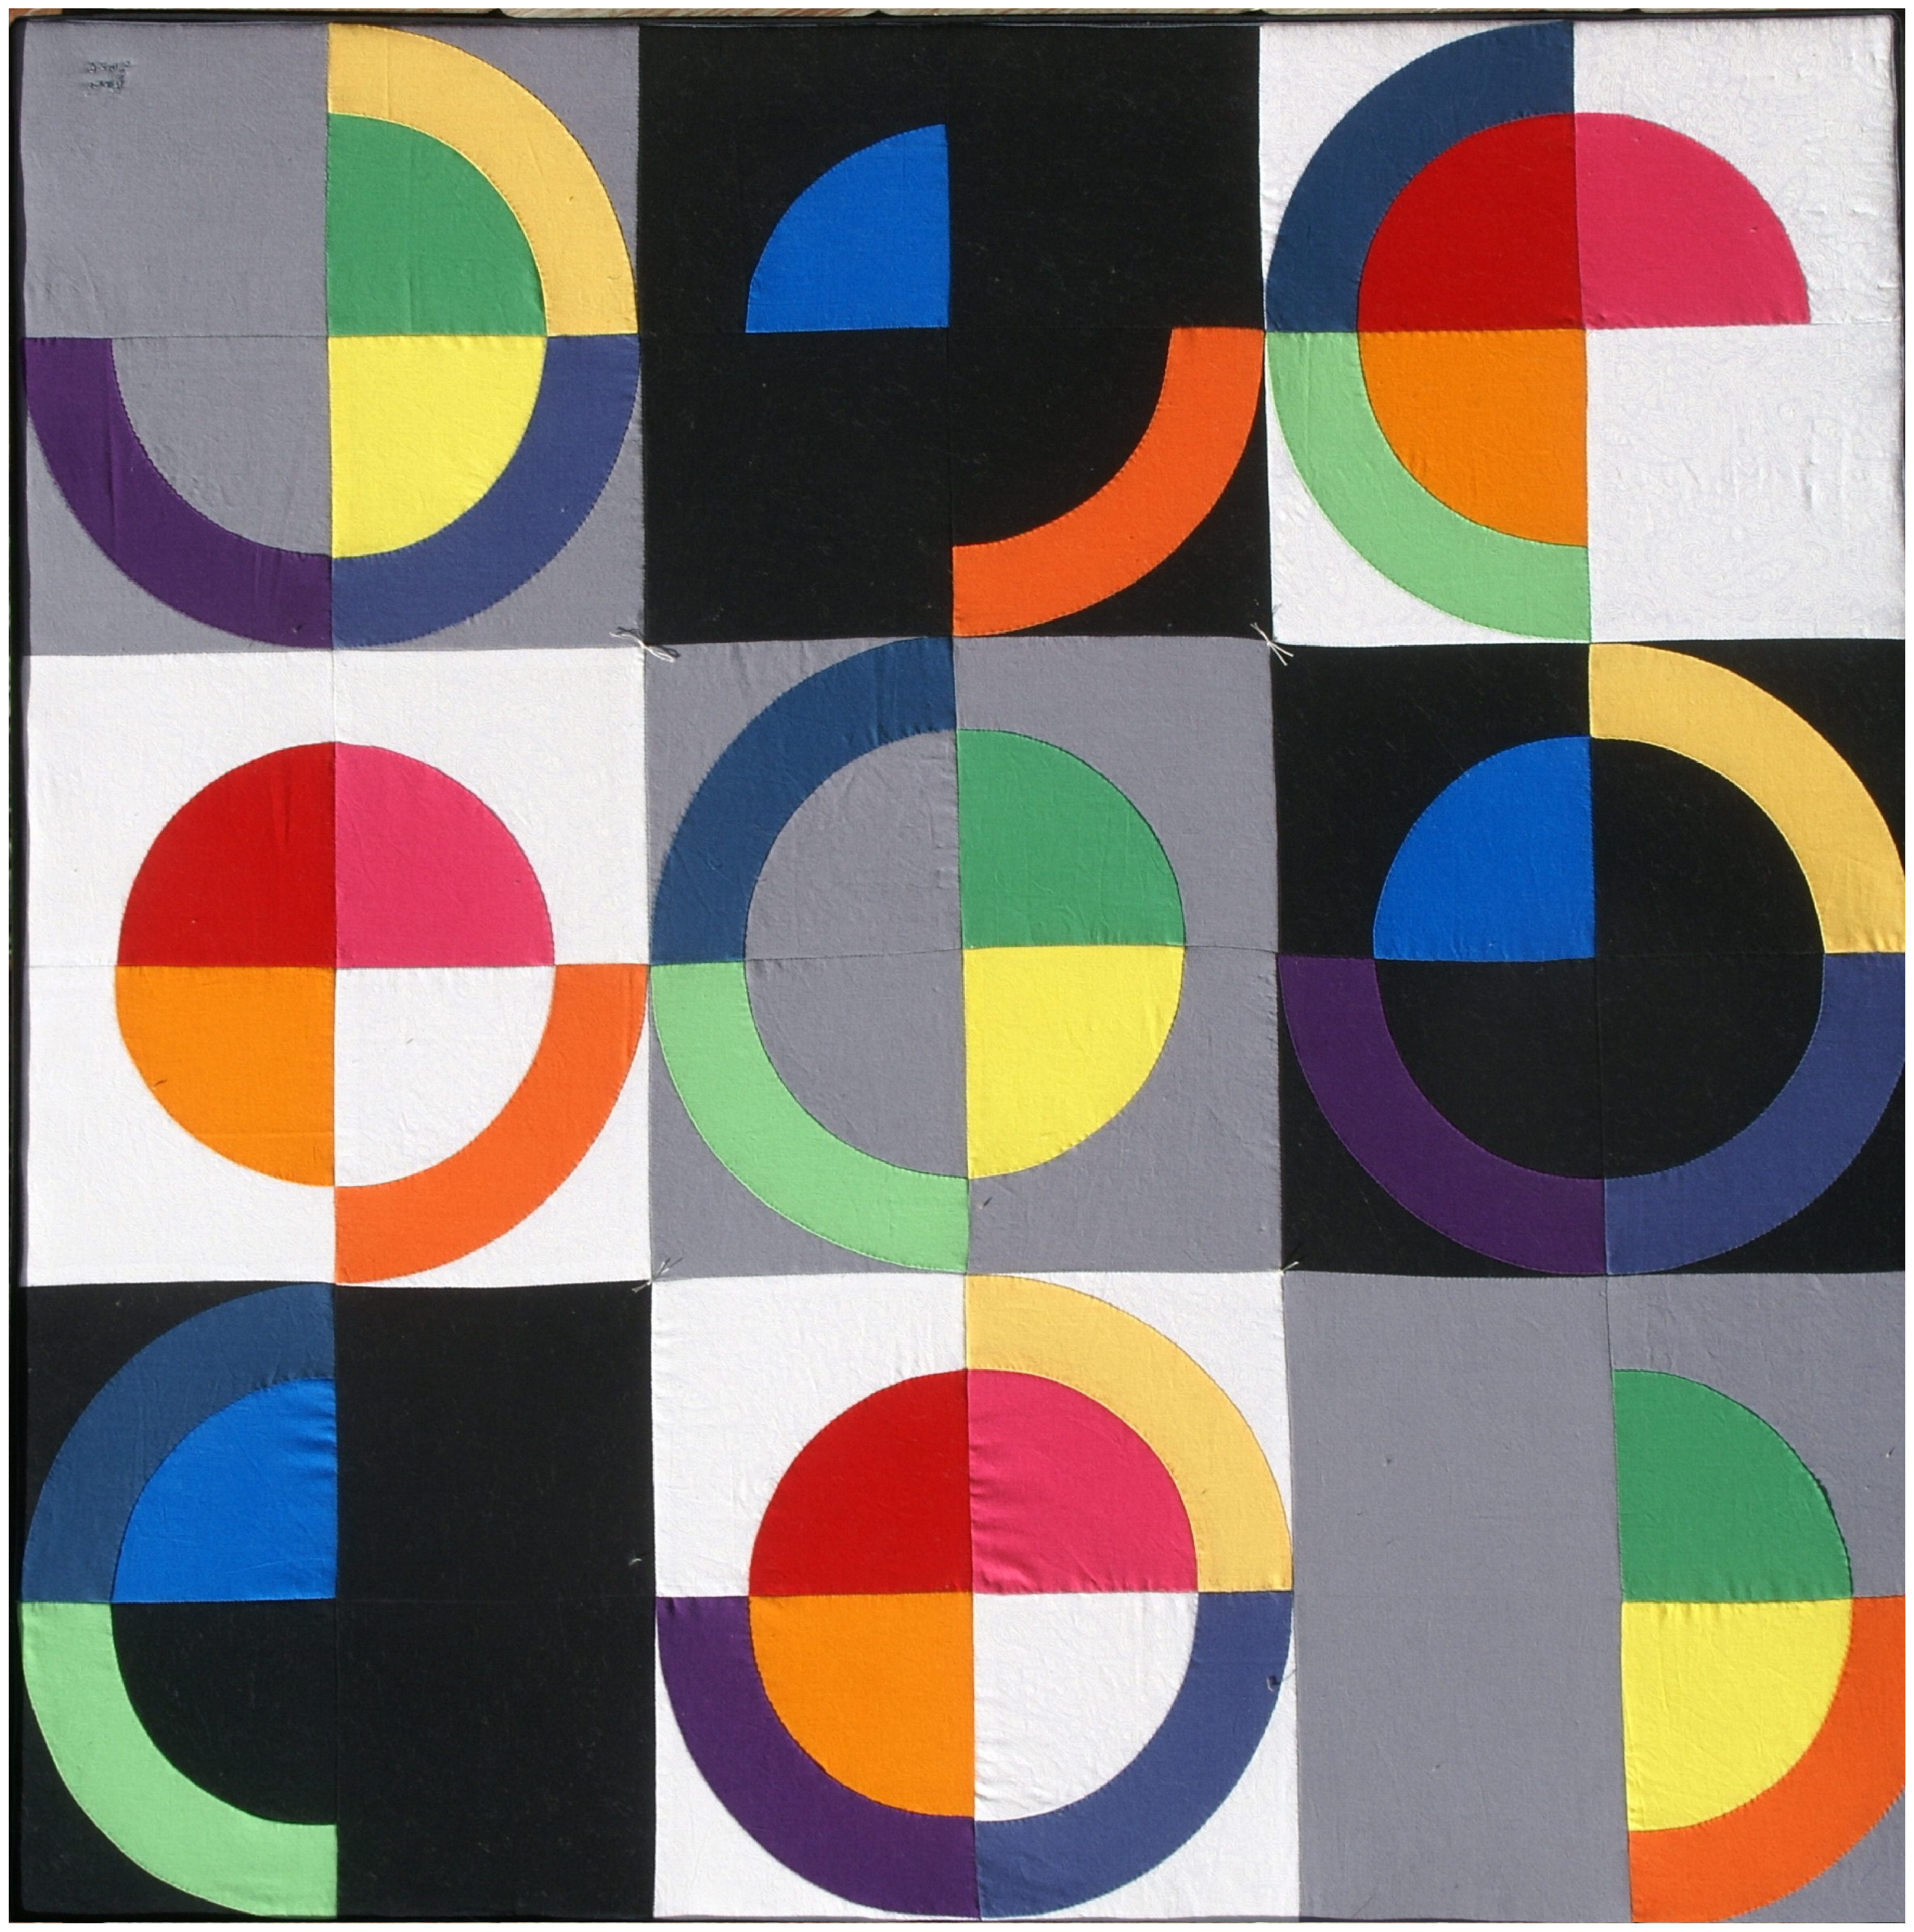
\epsfig{file=Florey.eps,height=151mm}%203mm103mm

\end{flushright}

\setcounter{page}{1}

\newpage

\normalsize\

\vfill

\hfill \copyright\ \sort{Dines Bj{\o}rner \& Yang ShaoFa. \todaytime}
  

\newpage 

\ \vspace{4cm}

\noindent
\sort{Dines Bj{\o}rner and Yang ShaoFa}

\vspace{6mm} 

\noindent
\brcolor{\huge Domain Modelling}

\vspace{6mm} 

\noindent
\bbcolor{\Large A Primer}\footnote{Primer: A small introductory book
  on a subject [\texttt{https://www.merriam-webster.com/}]} 

\newpage

\noindent\sf
Dines Bj{\o}rner \hfill Yang ShaoFa\\[2mm]
DTU Compute \hfill Institute of Software\\
Technical University of Denmark \hfill Chinese Academy of Sciences\\
DK-2800 Kgs.Lyngby, Denmark \hfill 4th Zhongguancun South Fourth Street\\[2mm]
Fredsvej 11, DK-2840 Holte, Denmark \hfill Beijing, China\rm

\newpage


%%%%%%%%%%%%%%%%%%%%%%%%%%%%%%%%%%%%%%%%%%%%%%%%%%%%%%%%%%%%%%%%%%%%
%%%%%%%% Released for translation     10.4.2023 %%%%%%%%%%%%%%%%%%%%
%%%%%%%% Re-released for translation  22.6.2023 %%%%%%%%%%%%%%%%%%%%
%%%%%%%% Re-released for translation 26.12.2023 %%%%%%%%%%%%%%%%%%%%
%%%%%%%% Re-released for translation 04.01.2024 %%%%%%%%%%%%%%%%%%%%
%%%%%%%%%%%%%%%%%%%%%%%%%%%%%%%%%%%%%%%%%%%%%%%%%%%%%%%%%%%%%%%%%%%%

\noindent
\brcolor{\LARGE Prefacio}\label{primer-preface}\label{preface} 
\addcontentsline{toc}{section}{\brcolor{Prefacio}}
\minitoc
 
\begin{flushright}\label{front-Dogma}
\sort{El Dogma del Tríptico}\\[4mm]
\addcontentsline{toc}{subsection}{\bbcolor{El Dogma del Tríptico}}
\sf Para \textsl{especificar} \bmcolor{software},\\
\sf debemos entender sus requisitos.\\[1mm]
\sf Para \textsl{prescribir} \bmcolor{requisitos}\ysfchg{,}\\
\sf debemos entender el \bmcolor{dominio}.\\[1mm]
\sf Por lo tanto, debemos \bbcolor{estudiar, analizar} y \bbcolor{describir} los dominios.
\end{flushright}\rm%
\index{pdefind}{El Dogma del Tríptico}\index{pdefind}{Tríptico!Dogma, El}%\index{pdefind}{Dogma, El Tríptico}

\subsection*{\bbcolor{Dominios -- ¿Qué Son?}}
\addcontentsline{toc}{subsection}{\bbcolor{Dominios -- ¿Qué Son?}}

\pos{\normalsize}{\HHHH}


\label{1stdd}
\ysf{\domaindefinition}
\pos{\psno}{\mnewfoil}

\renewcommand{\newdbsquare}{\dbsquare}

\begynd
\pind \sort{Ejemplos} \ysfchg{d}e dominios son:
\begynd
\pind {\sl transporte ferroviario, por carretera, marítimo y aéreo;
\pind tuberías de agua, petróleo y gas;
\pind manufactura industrial;
\pind la industria de servicios financieros: clientes, bancos, tarjetas de crédito, acciones, etc.;
\pind mercados de consumo, minorista y mayorista;
\pind atención médica;}
\pind etcétera.
\afslut
\afslut
\subsection*{\bbcolor{Meta y Objetivos}}\addcontentsline{toc}{subsection}{\bbcolor{Meta y Objetivos}}  

\vspace*{-4mm}

\begin{itemize}
      \item La \sort{meta} de esta \monografía\ es contribuir a una 
      metodología para analizar y describir dominios.
  
\item Los \sort{objetivos} -- en el sentido de `cómo se logra la meta' -- se reflejan en la estructura y el contenido
      y el enfoque didáctico de esta \monografía.
\item Los elementos principales de \ysfchg{nuestro} enfoque -- a lo largo de un
  eje conceptual -- se pueden enumerar: 
\begin{itemize}
\item Está el fundamento de nuestro enfoque de análisis y descripción
      en proporcionar una base \sort{filosófica},
      cf.\,capítulo\,\ref{chap2.tex.Philosophy}. 
\item Está la aplicación de ideas de \sort{taxonomía} 
      para entender la estructuración posiblemente jerárquica
      de los fenómenos del dominio, logrando una comprensión de las propiedades
      de los fenómenos y las relaciones entre ellos.
\item Están las nociones de \sort{endurantes} y \sort{perdurantes} -- % After giving it some thought, I think I align with "making up" the endurante and perdurante terms and just addding a footnore clariying what they mean.
      con los \sfsl{endurantes}  \index{pdefind}{endurante} siendo los fenómenos
\begynd
\pind que pueden ser observados, o concebidos y descritos, como \nyl una ``cosa completa'' en cualquier instante dado de tiempo\pos{
      \cite[vol.\,I, pág.\,656]{OED}}{},
\afslut
      y los \sfsl{perdurantes}  \index{pdefind}{perdurante} siendo los fenómenos 
\begynd
\pind de los cuales solo existe un fragmento\pos{}{\\} si los observamos o
      los tocamos\pos{}{\\} en cualquier instante dado de tiempo\pos{
      \cite[vol.\,II, pág.\,1552]{OED}}{}.
\afslut
\item Está la introducción de elementos base de
      \sort{cálculos}  \index{pdefind}{cálculos} para analizar y
      describir dominios. \index{pdefind}{cálculo!análisis}
\item Está la aplicación de ideas de \sort{ontología} 
      para entender la estructuración posiblemente jerárquica
      de estos cálculos.\index{pdefind}{ontología} 
\item Finalmente, está la noción de la
      \index{pdefind}{deducción trascendental} \sort{deducción
      trascendental}, cf.\,Sect.\,\ref{sec:Transcendence}, para ``transformar''
      ciertos tipos de endurantes en ciertos tipos de perdurantes,
      capítulo \ref{chap6.tex.1}.
\end{itemize}
\item A lo largo de otro eje conceptual, tenemos los siguientes elementos adicionales
        de nuestro enfoque:
\begin{itemize}
\item Consideramos que las descripciones de dominio, las prescripciones de requisitos y
      las especificaciones de diseño de software son cantidades \brcolor{matemáticas}
      \index{pdefind}{matemáticas}.
\item Las consideramos básicamente en el sentido de la
      \sort{teoría de funciones recursivas}
      \index{pdefind}{teoría de funciones recursivas} \cite[Hartley Rogers,
      1952]{Rogers67} y  la
      \sort{teoría de tipos}  \index{pdefind}{teoría de tipos} \cite[Benjamin
      Pierce, 1997]{pierce1997}.  
\end{itemize}
\end{itemize}

\vspace*{-4mm}
\subsection*{\bbcolor{Metodología}}\addcontentsline{toc}{subsection}{\bbcolor{Metodología}}\label{front:Methodology}

\begynd
\pind Por \sort{método} entenderemos
\begynd
\pind un conjunto de \sort{principios}\index{pdefind}{principio}
\footnote{Por \sort{principio} nos referimos a:
  \sfsl{un principio es una proposición o valor que sirve como guía para
    el comportamiento o la evaluación \wiki, es decir, un código de conducta}}
y \sort{procedimientos}\index{pdefind}{procedimiento}%
\footnote{Por 
  \sort{procedimiento} nos referimos a: \sfsl{instrucciones o recetas, un conjunto de comandos
    que muestran cómo lograr algún resultado, como preparar o hacer
    algo \wiki, es decir, una forma establecida de hacer algo}} 
\pind para seleccionar y aplicar un conjunto de
\sort{técnicas}\index{pdefind}{técnica}%
\footnote{Por \sort{técnica} nos referimos a: \sfsl{una técnica, o destreza, es
    la capacidad aprendida para realizar una acción con resultados determinados
    con buena ejecución, a menudo dentro de una cantidad de tiempo y energía
    dada, o ambas \wiki, es decir, una manera de
    llevar a cabo una tarea particular}}
y \sort{herramientas}\index{pdefind}{herramienta}%
\footnote{Por 
  \sort{herramienta} nos referimos a: \sfsl{una herramienta es un objeto que puede extender la
    capacidad de un individuo para modificar características del entorno
    circundante \wiki}} a un problema  
\afslut
\pind para lograr una construcción ordenada de una
      \sort{solución}, es decir, un \sort{artefacto}.
\afslut
\mnewfoil
\begynd
\pind Por \sort{metodología} entenderemos
\begynd
\pind el \sfsl{estudio \& aplicación} de uno o más métodos.
\afslut
\afslut
\mnewfoil

\pind Por \sort{método formal} entenderemos un método
\begin{itemize}
\item cuyos \sfsl{principios} incluyen considerar sus artefactos como % I don't understand the original meaning of this paragraph
      cantidades \sfsl{matemáticas}, como \sfsl{abstracciones}, etc.;
\item cuyos \sfsl{procedimientos} decisivos incluyen
\begin{itemize}
\item el análisis
      \ysfchg{\&} descripción secuencial primero de los endurantes, seguido por los perdurantes,
      y,
\item dentro del análisis \ysfchg{\&} descripción de los endurantes,
      el análisis \ysfchg{\&} descripción secuencial primero de sus cualidades externas y luego de sus cualidades internas,
\item etc.;
\end{itemize}
\item cuyas \sfsl{técnicas} incluyen formas específicas de
       especificar propiedades; y
\item cuyas \sfsl{herramientas} incluyen uno o más
      \sort{lenguajes formales.} % Needs revision for conjunctions and punctuation :/
\end{itemize}
\mnewfoil

\noindent
\begynd
\pind Por \sort{lenguaje} entenderemos aquí \nyl un conjunto de
cadenas de caracteres, es decir, oraciones,
\begynd
\pind oraciones que están estructuradas según alguna \sort{sintaxis},
      es decir, \sort{gramática},
\pind a las que se les da significado por alguna \sort{semántica},
\pind y que se utilizan según alguna \sort{pragmática}. 
\afslut
\afslut

\begynd
\pind Por \sort{lenguaje formal} entenderemos aquí un lenguaje
\begynd
\pind cuya \sfsl{sintaxis} y \sfsl{semántica} pueden ser expresadas
      \sort{matemáticamente}
\pind y para cuyas oraciones se puede \sort{razonar racionalmente} % Unsure where we want an "and" here or if "probar propiedades" is the intended meaning.
      (\sfsl{argumentar, probar}) \sort{propiedades}. 
\afslut

\pind Nos referimos al capítulo\,1 de \cite{BjornerMonograph2020} para un conjunto de
      definiciones de conceptos de 8 páginas y aproximadamente 50 entradas como las anteriores.
      
\pind Nos referimos al índice de \textsf{Método}, sect.\,\vref{label.dadmethod}.
\afslut
      
\treprikker

\noindent
\pind En este \manual\ usaremos
\begynd 
\pind el lenguaje de especificación formal, \texttt{RSL},
\pind el \texttt{R}AISE\footnote{\sort{RAISE: "R}igorous
      \sort{A}pproach \ysfchgii{ }
      to \ysfchg{\sort{I}ndustrial } \sort{S}oftware \sort{E}ngineering" (enfoque riguroso de la ingeniería industrial), % This is hard to translate for me. 
      \cite{RaiseMethod}} \texttt{S}pecification 
      \texttt{L}anguage, \cite{RSL} -- 
\pind y nos basaremos notablemente en la adaptación de \texttt{RSL} de \sort{CSP}, los
      \sfsl{Procesos Secuenciales Comunicantes ("Communicating Sequential Processes")} de Tony Hoare \citecsp;
\pind y propagaremos un método definitivo para el estudio y
      descripción de dominios.
\afslut
\afslut

\subsection*{\bbcolor{Un Énfasis}}\addcontentsline{toc}{subsection}{\bbcolor{Un Énfasis}} 

\anemphasis{Los dominios exhiben endurantes y perdurantes. Un modelo de dominio
  es, por lo tanto, algo que define los \sfsl{sustantivos} (hablando en términos generales, los
  endurantes) y los \sfsl{verbos} (hablando en términos generales, los {perdurantes}) -- y
  su combinación -- de un
  \sfsl{lenguaje} hablado y usado por escrito por los practicantes del dominio. No es una
  instanciación de sustantivos, verbos y su combinación,
  sino todas las posibles y sensatas instanciaciones.}{}

\subsection*{\bbcolor{Una Advertencia}}\addcontentsline{toc}{subsection}{\bbcolor{Una Advertencia}}

Los lectores experimentados de \texttt{RSL} \cite{RSL} podrían observar nuestro,
quizás despreocupado (informal), uso de \texttt{RSL}. Quizás, en algunos lugares, la 
sintaxis de las cláusulas de \texttt{RSL} no sea del todo correcta. Nuestro no uso
de los constructos de módulos (\texttt{Esquema}\ysfchg{, } \texttt{Clase} y \texttt{Objeto})
de \texttt{RSL} \ysfchg{nos} fuerza a declarar \textsf{canal}es de la misma manera
en que se introducen \textsf{tipo}s, \textsf{valor}es y \textsf{variable}s.

\begin{itemize}
%%\item[] \hfill 
\epsfig{file=db.eps,height=25mm}

%%\vspace*{-12mm}
\item[] \hfill   Dines Bj{\o}rner \& Yang ShaoFa

\item[] \hfill \todaytime
\end{itemize}


\label{preface.n}
%%  LocalWords:  analyse defind artefactual et cetera analysing RSL
%%  LocalWords:  endurants perdurants endurant perdurant Hartley AISE
%%  LocalWords:  pdefind artefact artefacts dadmethod igorous pproach
%%  LocalWords:  oftware ngineering pecification anguage CSP Hoare's
%%  LocalWords:  instantiation instantiations ndustrial Bj rner
%%  LocalWords:  ShaoFa


\addcontentsline{toc}{subsection}{\brcolor{Table of Contents}}
\setcounter{tocdepth}{1}
\dominitoc
\tableofcontents
\addcontentsline{toc}{subsection}{\brcolor{End of Table of Contents}}

%%  LocalWords:  Bj rner Modelling DTU DK Kgs Lyngby Fredsvej Holte


\mainmatter

\nbbbbbb{Introducción}\label{chap:Introduction}\label{chap:Introduction.1}
\minitoc

\begin{flushright}\label{intro:The Triptych Dogma}
\sort{El Dogma del Tríptico}\\[4mm]
\addcontentsline{toc}{subsection}{\bbcolor{El Dogma del Tríptico}}
\sf Para \textsl{especificar} \bmcolor{{$\mathcal{S}$}oftware},\\
\sf debemos entender sus requisitos.\\[1mm]
\sf Para \textsl{prescribir} \bmcolor{{$\mathcal{R}$}equisitos},\\
\sf debemos entender el \bmcolor{$\mathcal{D}$ominio}.\\[1mm]
\sf Así que debemos \bbcolor{estudiar, analizar} y \bbcolor{describir} dominios.\\
\end{flushright}\rm%
\index{pdefind}{El Dogma del Tríptico}\index{pdefind}{Dogma del Tríptico, El}\index{pdefind}{Dogma, El Tríptico}
\mnewfoil

\boiteepaisseavecuntitre{$\mathcal{D},\mathcal{S}\models\mathcal{R}$}
\noindent
\begynd
\pind En pruebas de corrección ($\models$) % "Corrección" needs revision %
\begynd
\pind de $\mathcal{S}$oftware
\pind con respecto a $\mathcal{R}$equisitos,
\pind las suposiciones a menudo se establecen \ysfchg{con respecto al } $\mathcal{D}$ominio.
\afslut
\pind Esto por sí solo justifica nuestro enfoque en los dominios.
\afslut
\endboiteepaisseavecuntitre

\mnewfoil

\noindent
\begynd
\pind \ysfchgii{Este} \manual\ es
\begynd
\pind tanto una versión significativamente reducida \nyl de la monografía científica \cite{BjornerMonograph2020} 
\pind como una revisión y, notablemente, simplificación, de algunos de sus hallazgos.
\afslut
\afslut

\nbbbbb{¿Porqué este manual?}\label{sec:Why This Primer}

\begynd
\pind Este \manual\ está pensado como un \sort{libro de texto}.
\pind Los cursos que \ysfchg{tenemos} en mente, durante sus \sort{conferencias}, se deben \sort{enfocar} en los
      Capítulos\,\ref{chapter:Domains}--\ref{chapter:Perdurants},
      es decir, Páginas\,\pageref{chapter:Domains}--\pageref{chapter:Perdurants.n}.
\pind Se espera que los \sort{estudiantes aplicados}, ya sean solo lectores o matriculados del curso, estudien
      los Capítulos\,\ref{chap:Introduction}--\ref{chapter:Philosophy} así
      como el Capítulo\,\ref{chapter:Closing}, la Bibliografía
      (Capítulo\,\ref{primer.bib}) y los apéndices por su propia cuenta\,!
\afslut

\begynd
\pind  \ysfchgii{Este} \manual\ trata sobre cómo \sfsl{analizar \& describir} dominios artificiales
      (incluyendo su posible interacción con la naturaleza).
      \pind Enfatizamos el ampersand: `\&'.\footnote{Al no escribir `y', sino `\&', enfatizamos que en
      ${A\&B}$ estamos tratando con un \sort{único} concepto que consiste en
      tanto $A$ como $B$ ``interactuando estrechamente''.}
\pind Justificamos la competencia en \sfsl{Ciencia e Ingeniería de Dominios}
      por dos razones.
\begynd
\pind (i) Por motivos de un \sfsl{desarrollo de software siguiendo buenas prácticas de ingeniería} -- como se indica por el \sort{Dogma del Tríptico} mencionado anteriormente. En  %This sentence seriously needs revision. Unsure about original intention of the english sentence
      posibles pruebas de propiedades del software se hacen referencias, no
      solo al código del software en sí y a los requisitos, sino también
      al dominio en forma de \sfsl{suposiciones sobre este mismo}. En nuestra opinión, ningún proyecto de desarrollo de software debería
      emprenderse a menos que comience más o menos con una etapa adecuada de ingeniería
      de dominio. Y
\pind (ii) por motivos de \sfsl{comprender científicamente} nuestro propio
      mundo práctico cotidiano: instituciones financieras, la industria del transporte
      (tráfico por carretera, ferroviario y aéreo, envío), sistemas de alimentación
      (como sistemas de tuberías de petróleo, gas, agua y otros), etc.
\afslut
\afslut


\nbbbbb{Structure}\label{sec:Structure}

\begynd
\pind The \primer, beyond the present chapter, has, syntactically
speaking, three elements:
\afslut

\begin{enumerate}
\item \sort{Chapter\,\ref{chap2.tex.Philosophy}} covers the \sfsl{philosophy} of
      \texttt{Kai S{\o}rlander}
      \cite{kaisorlander1994,kaisorlander1997,kaisorlander2002,kaisorlander2016,kaisorlander2022}.

      Yes, a major contribution of \cite{BjornerMonograph2020} and
      this \primer\ is to justify important domain concepts by
      their sheer inevitability in any world description.
      
\item \sort{Chapters\,\ref{chapter:Domains}--\ref{chapter:Perdurants}} presents \sfsl{the methodology of
    domain engineering.} It is split into four chapters for practical
    and pragmatic
    reasons. Chapter\,\ref{chapter:Domains} gives a ``capsule
    introduction'' into Chapters\,\,\ref{primer-extq.1}--\ref{chapter:Perdurants}.
  
\item \sort{Chapters\,\ref{chapter:Closing}--\ref{primer.bib}}
  and \sort{Appendices\,\ref{Chapter:Road Transport}--\ref{primer.indexes}} cover
  such things as `closing remarks' (\sort{\ref{chapter:Closing}}), a `bibliography' (\sort{\ref{primer.bib}}), a `Road
  Transport' example (\sort{\ref{Chapter:Road Transport}}), a `Pipeline System' example (\sort{\ref{appendix:Pipelines}}), an `\texttt{RSL}
  formal specification language' primer (\sort{\ref{RSL-intro}}), and `Indexes' to definitions, concepts, etc. (\sort{\ref{primer.indexes}}).
\end{enumerate}

\nbbbbb{Prerequisite Skills}\label{Prerequisite Skills}

\begynd
\pind The \pos{reader}{course student} is expected to possess the
      following skills:
\afslut
\begin{itemize}
\item To be reasonably versed in \sort{discrete mathematics:} mathematical logic
  and set theory.
\item To have had, even if only a  fleeting, acquaintance with abstract
  specifications in the style of
  \texttt{VDM} \citevdm,
  \texttt{Z} \citez,
  \texttt{CafeObj} \citecafeobj, 
  \texttt{Maude} \cite{maude-primer,maude-manual}, or the like -- and thus
  to enjoy abstractions\footnote{Some say: \sfsl{``Mathematics is the
  Science of Abstractions''}\,! Others say that both \sfsl{``Mathematics and
  Physics are Abstractions of Reality''}.}.
\item To have reasonable experience with \sort{functional programming} a
      la \texttt{Standard ML} or \textsf{F}
      \cite{MilnerTofte,Harper,MRHansen+HRischel} respectively
      \cite{Hansen+Rischel} -- or similar such language.
    \item To have  reasonable experience with \sort{\texttt{CSP}}
      \cite{Hoa78,Hoare85,Hoare85+2004,Roscoe97,Schneider99}.
\end{itemize}
\noindent
\begynd
\pind The \pos{reader}{course student} is further expected to possess
      the following mindset:
\afslut
\begin{itemize}
\item To basically consider software as\ \sort{mathematical
      objects}. That is: as quantities about which one can (and must) reason logically.
  \item To \sort{think and ``act'' abstractly}. An essence of
  abstraction is expressed in the next section.

\item To \sort{act responsibly}\footnote{It is, today, \todaytime, 
    very fashionable to propagate messages of `ethics' to programmers
    -- without even touching upon issues such as \sfsl{``have You
    understood Your application domain thoroughly\,?''}, or
    \sfsl{``have You reasoned about adequacy of your requirements\,?''},
    or \sfsl{``have You model-checked, proved and formally tested your
    specifications (descriptions and prescriptions) and Your
    code\,?''}, etc.}, that is to make sure that You have 
    indeed understood Your domain, that You  have indeed reasoned
    about adequacy of your requirements, and  You have indeed
    model-checked, proved and formally tested Your  
    specifications.
\end{itemize}

\nbbbbb{Abstraction}\label{primer:Abstraction}

%\input{abstraction}

\QUOTATION{Conception, my boy, fundamental brain-work, \\ 
           is what makes the difference in all art\ysf{.}}%
          {D.G.\ Rossetti\footnote{Dante Gabrielli Rosetti,
          1828--1882, English poet, illustrator, painter and
          translator.}: letter to T.\ H.\ Hall Caine\footnote{T.\ H.\ Hall Caine,
          1853--1931, British novelist, dramatist, short story
          writer, poet and critic.}}  

\pos{\psno}{\mnewfoil}

\noindent
\pos{}{Quoting \sort{C.A.R.\,Hoare:}}

\noindent
\begynd
\pind {\sl Abstraction is a tool,
\begynd
\pind used by the human mind, 
\pind and to be applied in the process of describing \nyl 
          (understanding) complex phenomena.
\afslut
}

\pind {\sl Abstraction is the most powerful such tool  \nyl
available to the human intellect.}

\pind {\sl Science proceeds by simplifying reality. }
\begynd
\pind {\sl The first step in simplification is abstraction.}
\pind {\sl Abstraction (in the context of science) \nyl  
          means leaving out of account all those empirical \nyl
          data which do not fit the particular, conceptual 
          framework \nyl within which science at the moment
          happens to be working.}
\afslut
\afslut

\pos{\psno}{\mnewfoil}
\begynd
\pind {\sl Abstraction (in the process of specification)}
\begynd
\pind {\sl arises from a conscious
          decision
\pind  to advocate certain 
          desired objects, situations and processes
\pind  as being fundamental; 
\pind by exposing, 
          in a first, or higher, level of
          description, their similarities 
\pind  and \ysf{--} at that level -- ignoring
          possible differences.}
\afslut
\afslut

  \ \hfill     \pos{ [From the opening paragraphs of}{} 
           \cite[C.A.R.\ Hoare\ysf{,} \textsl{Notes on Data
           Structuring}]{Hoa72a}\pos{\ysf{.}]}{}
       %}{}

\nbbbbb{Software Engineering}\label{sec:Software Engineering}
\bbbb{Domain Science \& Engineering}

\begynd
\pind This \primer\ covers only the \sfsl{application domain} of software development.
\pind There are two things to say about that.
\begynd
\pind One is that facets of \sfsl{requirements},
\begynd
\pind essential ones, is covered in \cite[Chapter 8]{BjornerMonograph2020},
\pind general ones in \cite[Software Engineering, III, Part V]{TheSEBook3};
\afslut
\pind the other is that the pursuit of developing domain models \nyl
      is not just for the sake of software development, \nyl
      but also for the sake of just understanding the man-made world
      around us.
\afslut
\pind Domain science and engineering can thus be pursued in-and-by itself.
\afslut

\nbbbb{Software Engineering}

\begynd
\pind In 2006 \ysfchg{these books were } published: \cite{TheSEBook1,TheSEBook2,TheSEBook3}:
\afslut

\begin{center}
\epsfig{file=SE1.eps,width=4cm}\ \
\epsfig{file=SE2.eps,width=4cm}\ \
\epsfig{file=SE3.eps,width=4cm}
\end{center}

\nbbb{Domain Engineering: 2016--2022}\label{Domain Engineering 2016 2022}

\begynd
\pind The first inklings of the domain science and engineering of
      \cite{BjornerMonograph2020} appeared in \cite[2010]{Kiev:2010ptI,Kiev:2010ptII}.
\pind More-or-less ``final'' ideas were published, first in \cite[2017]{BjornerFAoC2015MDAAD},
      then in \cite[March 2019]{BjornerTOSEM2018}.
\pind The book \cite{BjornerMonograph2020} with updates in this
      \primer, then constitutes the most recent status of our work in domain
      science \& engineering. 

\pind \cite[Software Engineering, III, Part V]{TheSEBook3} does not
      cover the \sfsl{Domain Engineering} material covered in
      \cite[Chapter 8: Domain Facets]{BjornerMonograph2020}.
\begynd
\pind That latter was researched \cite{dines:facs:2008} and developed between the appearance
      of \cite{TheSEBook3} and, obviously, \cite{BjornerMonograph2020}.
\afslut
\afslut

\begynd
\pind Part V of \cite{TheSEBook3}, except for Chapters\,17--18 is
      still relevant.
\pind Chapters\,17--18 of \cite{TheSEBook3} are now to be replaced in
      any study by Chapters\,4--7 of \cite{BjornerMonograph2020} \sort{or}
      this \primer\,!
\afslut

\nbbb{Requirements Engineering}

\begynd
\pind This \primer\ does not show You how to proceed into software
      development according to the \sort{Triptych Dogma}.
\begynd
\pind This is strongly hinted at in \cite[Chapter 9]{BjornerMonograph2020}.
\pind (That chapter is an adaptation of \cite[May 2008]{dines:ugo65:2008}.)
\pind Our approach to \sfsl{requirements engineering} is rather
      different from that of both \cite[A. van Laamswerde]{Lamsweerde}
      and \cite[M.\ A.\ Jackson]{Jackson2010Facs} -- to cite 
      two relevant works.
\pind It is, \ysfchg{we } strongly think, commensurate with these works.
\pind  \ysfchg{We } wish that someone could take up this line of research:
\begynd
\pind making more precise, perhaps more formal, the ideas of
      \sfsl{projection, intialisation, determination, extension} and \sfsl{fitting};
\pind and comparing, perhaps unifying our approach with that of
      Lamsweerde and Jackson.
\afslut
\afslut
\afslut

\nbbb{Software Design}

\begynd
\pind For the software design phase, after requirements engineering,
\pind we, of course, recommend \cite[\sfsl{Software Engineering}
      \ysfchgv{V}ols.\,1--2]{TheSEBook1,TheSEBook2} 
\afslut

\nbbbbb{The Structuring of The Text}\label{The Structuring of The Text}

\begynd
\pind The \pos{reader}{student} will find that this text consists of
      ``diverse'' kinds of usually small paragraphs of texts:
\begynd
\pind \bbcolor{definition}s -- properly numbered and labeled;
\pind \bbcolor{example}s -- properly numbered and labeled;
\pind \bbcolor{analysis predicate, function,} and
      \bbcolor{description prompt} ``formalisations'';
\pind \bbcolor{method} principle, procedure, technique and tool paragraphs;
\pind -- all of these delineated by closing {\dbsquare}s;
\pind -- with short, usually one or two small paragraphs of
      introductory or otherwise explaining texts.
\afslut
\pind All of \ysfchg{these are } \textsf{``brought to You in living
  colours''\,!}\footnote{\LLLL -- as the \textsf{NBC} Television
  Network programmmes would ``proudly'' announce in \ysf{t}he 1960s\,!}
\pind So be prepared:
\begynd
\pind Study such paragraphs: paragraph-by-paragraph.
\pind Each form\ysfchg{s } a separate ``whole''.
\afslut
\afslut


\nbbbbb{Self-Study}\label{sec:Used for Self-Study}

\begynd
\pind This \primer\ is primarily intended to support actual, physical lectures.
\pind For self-study by B.Sc.\ and M.Sc.\ students and practicing
      novice software engineers  we recommend to use this \primer\ in
      connection with its ``origin'' \cite{BjornerMonograph2020}.
\pind For  self-study by Ph.D.\ students and graduated computer
      scientist we recommend going directly to the source:
      \cite{BjornerMonograph2020}.   
\afslut

\nbbbbb{Two Examples}\label{primer:Two Examples}

\begynd
\pind There are around 80 examples, scattered all over the first 120 pages.
\pind In addition we bring two larger examples:
\afslut
\begin{itemize}
\item \textsf{Road Transport}, Appendix\,\ref{Chapter:Road
        Transport}, pages\,\pageref{Chapter:Road Transport}--\pageref{p-ch:Road Transport.n}, 
\item \textsf{Pipelines},
      Appendix\,\ref{appendix:Pipelines}, pages\,\pageref{appendix:Pipelines}--\pageref{appendix:Pipelines.n}. 
\end{itemize}

\dbeat{%%%%%%%%%%%%%%%%%%%%%%%%%%%%%%%%%%%%%%%%%%%%%%%%%%%%%%%%%%%%%%%%%%%%%%%%%%%%%%%%%%%%%%%%%%%%%%
\nbbbbb{Lectures}\label{sec:Use in Lectures}

\begynd
\pind This \primer\ was developed during the summer of 2022.
\pind The author was to give a set of seven double lectures \nyl at the Technical
      University of Vienna\footnote{The author ``woke up'' to what
        software engineering and computer science is really about in
        Vienna, in 1973--1975 -- at the \sort{IBM Vienna Labor}, with
        colleagues like \sfsl{Hans Beki{\v{c}}, Cliff Jones, Peter Lucas} and \sfsl{Kurt Walk}. It
        had to be Vienna, the city of the \sfsl{Wiener Kreis}
        \texttt{en.\-wiki\-pedia.\-org/\-wi\-ki/\-Vienna\_\-Circle}, \sfsl{Ludwig
          Wittgenstein}
        \texttt{en.\-wiki\-pedia.\-org/\-wi\-ki/\-Lud\-wig\_\-Witt\-gen\-stein}
        and \sfsl{Sir Karl
          Popper}
        \texttt{en.\-wiki\-pedia.\-org/\-wi\-ki/\-Karl\_\-Popper}.}
      October
        24 -- November 4, 2022.
      \pind These lectures were: 
\begin{itemize}
\item Week 1:
\begin{description}
\item[Lecture Day 1:] Chapter\,\ref{chapter:Domains}:
\begin{itemize}
\item \sort{Domains} -- lecture ``doubles'' as a Faculty Seminar\,!
\end{itemize} and Appendix\,A: 
\begin{itemize}
\item \sort{An Example, I}
\end{itemize}
\item[Lecture Day 2:] Chapter\,\,\ref{primer-extq.1}:
\begin{itemize}
\item \sort{Endurants: External Qualities}
\end{itemize}
  
\item[Lecture Day 3:] Sections\,\,\ref{chap4.Internal
    Qualities}--\ref{chap4.Mereology}:
\begin{itemize}
\item \sort{Unique Identifiers}
\item \sort{Mereology}
\end{itemize}

\item[Lecture Day 4:] Sections\,\,\ref{chap4.Attributes}--\ref{A
    Domain Discovery Process, II}:
\begin{itemize}
\item \sort{Attributes},
\item \sort{Intentional Pull},
\item \sort{A Domain Discovery Process}
\end{itemize}
\end{description}
\item Week 2:
\begin{description}
\item[Lecture Day 5:]  Appendix\,A: 
\begin{itemize}
\item \sort{An Example, II}  Further on \sort{Road Transport}, and
\end{itemize}
 Chapter\,\,\ref{chapter:Perdurants}, Sect.\,\ref{A General Analysis of Part  Behaviours}:
\begin{itemize}
\item \sort{A General Analysis of Part Behaviours}
\end{itemize}
\item[Lecture Day 6:] Chapter\,\,\ref{chapter:Perdurants},
  Sects.\,\ref{Domain Channel Description}--\ref{Behaviour Definition Bodies}: 
\begin{itemize}
\item \sort{Channels} and
\item \sort{Behaviours Definitions: Signatures and Bodies}
\end{itemize}
\item[Lecture Day 7:] Chapter\,\,\ref{chapter:Perdurants},
  Sects.\,\ref{Domain Behaviour Initialisation}--\ref{A Domain Discovery Process, III}:
\begin{itemize}
\item \sort{Domain Behaviour Initialisation}, 
\item \sort{A Domain Discovery Process},
\end{itemize}
\end{description}
\end{itemize}
\afslut
}%%%%%%%%%%%%%%%%%%%%%%%%%%%%%%%%%%%%%%%%%%%%%%%%%%%%%%%%%%%%%%%%%%%%%%%%%%%%%%%

\nbbbbb{Relation to \cite{BjornerMonograph2020}}

\begynd
\pind This \primer\ is based on \cite[Nov.\,2021]{BjornerMonograph2020}.
\pind Chapter\,\ref{chapter:Philosophy} is a complete rewrite of
      \cite[Chapter\,2]{BjornerMonograph2020}.  
\pind Chapters\,\ref{primer-extq.1}--\ref{chapter:Perdurants} is a
      ``condensation'' of \cite[Chapters\,4--7]{BjornerMonograph2020}:
\begynd
\pind \cite[Chapter\,6]{BjornerMonograph2020} has been shortened and
      appears in this \primer\ as Sect.\,\ref{Transcendental Deductions}.
\pind From \cite[Chapter\,4]{BjornerMonograph2020} we have, in
      Chapter\,\ref{primer-extq.1}, omitted all 
      material on -- what is there referred to as \sfsl{Conjoins}.
\pind And we have further sharpened the notion of \sfsl{type names}.
\afslut
\pind We have sharpened the focus on methods: principle, procedures,
      techniques and tools.
\begynd
\pind You will find, in the \sfsl{Indexes} section,
      Sect.\,\vref{label.dadmethod}, a summary of references to these.
\pind Work is still in progress on highlighting more of the method steps.
\afslut
\pind Section\,\ref{Discrete Dynamic Domains} is new. 
\afslut

\nbbbbb{The \texttt{RAISE} Specification Language, \texttt{RSL}, and \rslplus}\label{RSL-I}

\begynd
\pind The formal notation (to go with the informal text) of this
      \primer\ is that of \texttt{RSL} \cite{RSL}, the \sort{R}AISE
      \sort{S}pecification \sort{L}anguage, where \texttt{RAISE}
      stand\ysfchg{s }
      for \sort{R}igorous \sort{A}pproach to \sort{I}ndustrial
      \sort{S}oftware \sort{E}ngineering \cite{RaiseMethod}. 
\pind Other formal notations could be used instead.
\pind Replacement examples could be \texttt{VDM} \citevdm , \texttt{Z}
      \citez, or \texttt{Alloy} \citealloy.
\pind We are more using the \texttt{RAISE} specification language,
      \texttt{RSL} than using the method.
\pind And we are using it in two ways:
\begin{itemize}
\item Informally, to present and explain the domain analysis \&
      description methods of this \primer, and
\item formally, to present domain descriptions. 
\end{itemize}
\pind The informal \texttt{RSL} is an extended version,
\rslplus.\footnote{See Appendix Sect.\,\vref{chap2.tex.rsltext}.}
\pind The two ways are otherwise not related.
\pind One could use another specification language \ysfchg{either } for the
      informal or \ysfchg{for } the formal aspects.
\afslut

\nbbbbb{Closing}

\begynd
\pind The purpose of this introduction is to place the present \primer\
\pind in the context of \ysfchgv{Dines Bj{\o}rner's } other books
      \cite{TheSEBook1,TheSEBook2,TheSEBook3} on software development 
\pind and possible lectures and self\ysf{-}study.
\afslut

\label{chap:Introduction.n}

%%  LocalWords:  analyse defind VDM CafeObj CSP Kai rlander RSL Ph wi
%%  LocalWords:  summarises Laamswerde intialisation Lamsweerde Beki
%%  LocalWords:  Kreis pedia ki Lud Endurants Mereology Behaviours
%%  LocalWords:  Behaviour Initialisation formalisations colours AISE
%%  LocalWords:  programmmes dadmethod pecification anguage igorous 
%%  LocalWords:  pproach ndustrial oftware ngineering Gabrielli Caine
%%  LocalWords:  Rosetti Hoare equirements omain pdefind wrt
    % Introduction
 
 

%%%%%%%%%%%%%%%%%%%%%%%%%%%%%%%%%%%%%%%%%%%%%%%%%%%%%%%%%%%%%%%%%%%%
%%%%%%%% Released for translation 11.4.2023, 13:00 %%%%%%%%%%%%%%%%%
%%%%%%%% Re-released 22.6.2023, 14:45 %%%%%%%%%%%%%%%%%%%%%%%%%%%%%%
%%%%%%%%%%%%%%%%%%%%%%%%%%%%%%%%%%%%%%%%%%%%%%%%%%%%%%%%%%%%%%%%%%%%

\pos{\nbbbbbb{ La Filosofia de Kai S{\o}rlander}}{}\label{chap2.tex.Philosophy}\label{chapter:Philosophy}
\minitoc

\index{pconind}{philosophy!S{\o}rlander's|(}

\bookdefn{Filosofia}{\ysfchgii{Filosofia }\pdefindex{filosofia}\footnote{\HHHH Del Griego:
      $\phi\iota\lambda{o}\sigma{o}\phi\iota\alpha$, philosophia, 'amor a la sabiduria'} % φιλοσοφία
\begynd
\pind is the study of general and fundamental questions es el estudio de preguntas generales y fundamentales, como 
\pos{}{\begin{multicols}{3}}
\begynd
\pind la existencia,
\pind el razonamiento,
\pind el conocimiento,
\pind los valores,
\pind la mente y
\pind el lenguaje \pos{\footnote{\LLLL Muchas de las `definiciones' en este \primer\ son en el estilo usado en filosofía. No son del estilo `preciso' utilizado comúnmente en las matemáticas y ciencias computacionales. Usted podrá querer llamarlo 
      \textbf{caracterización}es.
      

En matemáticas y ciencias computacionales el definidor tipicamente tiene una base formal en la cual construir. En las ciencias y ingeneria del dominio nosotros no tenemos una base formal, tenemos el mundo ``material'' de fenómenos naturales y hecho por el hombre.}}{}\dbsquare
\afslut
\pos{}{\end{multicols}}
\afslut
}

\pof{\nbbbbb{Introducción}}{}

\pof{}{\noindent}
\begynd
\pind En filosofando preguntas son hechas.
\pind Uno no necesariamente encuentra contestaciones a estas preguntas.
\begynd
\pind Preguntas son examinada.
\pind Light is thrown on the questions and their derivative questions. % 
\afslut
      
\pind Filosofia es el esfuerzo del hombre, nuestra mision,\nyl para  descrubir la necesaria caracteristicas de nuestro mundo y \nyl nuestra situacion como humano \ysfchg{en} ese mundo. 
\pind Nos enfocamos en el asunto de metafisica. \index{pconind}{metaphysics}%
\afslut

\mnewfoil
     
\begynd
\pind  El tratamiento en este \pof{capitulo}{paper}
\begynd
\pind esta basado en los escritos \nyl del filosofo daneses \bbcolor{\textsf{Kai S{\o}rlander}} (1944) \nyl
      \cite[1994--2022]{kaisorlander1994,kaisorlander1997,kaisorlander2002,kaisorlander2016,kaisorlander2022}
\pind en contraste y inspirado por \nyl el filosofo alemán
      \bbcolor{\textsf{Immanuel Kant}} (1724--1804) \cite{Kant1992}.
\afslut
\pind En 2023, en colaboración con \ysfchg{Kai } S{\o}rlander,
      \cite{kaisorlander2022} \ysfchg{fue traducido } al ingles \cite{kaisorlander2023}.
\afslut

\mnewfoil
      
\begynd
\pind La razón por la cual \ysfchg{nosotros}, como científicos de la computacion \ysfchg{deberíamos estar } interesado en filosofía,
\begynd
\pind es que filosofos por mas de 2500 años is that philosophers over more than 2500
      years{\footnote{\LLLL -- \label{citations-1}
      starting, one could claim, with:\scriptsize\footnotesize
\begin{multicols}{2}
\begin{itemize}
\item \sfsl{Thales of Milet} 624--545 [todo origina del 
      {\texttt{agua}}] \cite{Thales:Dines};
\item \sfsl{Anaximander} 610--546 [{\texttt{`apeiron'}} (the
      `un\--dif\-fer\-ren\-ti\-a\-ted', `the unlimited') is the
      origin] \cite{Anaximander:Dines};
\item \sfsl{Anaximenes} 586--526 [{\texttt{aire}}es la base de todo] \cite{Anaximenes:Dines};
\item  \sfsl{Heraklit of Efesos} 540--480 [\texttt{fuego} es la base y toda en la naturaleza {\texttt{se encuentra en una eterna ``pelea''}}]  \cite{Heraklit:Dines};
\item \sfsl{Empedokles} 490--430 [existen cuatro elementos bases:
      {\texttt{fuego, agua,aire}} y {\texttt{tierra}}] \cite{Empedokles:Dines};
\item \sfsl{Parminedes} 515--470 [todo lo que existe es \texttt{eterno y inmutable}] \cite{Parminedes:Dines};
\item \sfsl{Demokrit} 460--370 [todo es construido de {\texttt{atomos}}] \cite{Demokrit:Dines};
\item the Sophists: Protagoras, Gorgias (fifth and fourth centuries BC),
\item \sfsl{Socrates} (470--399) \cite{Socrates:Dines},
\item \sfsl{Plato} (424--347) \cite{Plato:Dines},
\item \sfsl{Aristotle} (384--322) \cite{Aristotle:Dines-x},
\item etcetera.
\end{itemize}
\noindent
Después de mas de 1800 años vinieron 
\begin{itemize}
\item \sfsl{Ren{\'e} Descartes} (1596--1650) \cite{Descartes:Dines},
\item \sfsl{Baruch Spinoza} (1632--1677) \cite{Spinoza:Dines},
\item \sfsl{John Locke} (1632--1704) \cite{Locke:Dines},
\item \sfsl{George Berkeley} (1685--1753) \cite{Berkeley:Dines},
\item \sfsl{David Hume} (1711--1776) \cite{Hume:Dines},
\item \sfsl{Immanuel Kant} (1724--1804) \cite{Kant:Dines},
\item \sfsl{Johan Gottlieb Fichte} (1762--1814) \cite{Fichte:Dines},
\item \sfsl{Georg Wilhelm Friedrich Hegel} (1770--1831) \cite{Hegel:Dines},
\item \sfsl{Friedrich Wilhelm Schelling} (1775--1864) \cite{Schelling:Dines},
\item \sfsl{Edmund Husserl} (1859--1938) \cite{Husserl:Dines},
\item \sfsl{Bertrand Russell} (1872--1970) \cite{Rus12,Russell1910-1913,Russell1905,Russell1919},
\item \sfsl{Ludwig Wittgenstein} (1889--1951) \cite{Wittgenstein21,Wittgenstein58},
\item \sfsl{Martin Heidegger} (1889--1976) \cite{Heidegger27},
\item \sfsl{Rudolf Karnap} (1891--1970) \cite{RudolfCarnap1928,Car37,Car42},
\item \sfsl{Karl Popper} (1902--1994) \cite{popper-tlosd59,popper-car-tgask63},
\item etcetera.
\end{itemize}
\end{multicols}
\noindent
(This list is ``pilfered''
      from \cite[Pages 33--127]{kaisorlander2016}.) \label{citations-2}
      \cite{kaisorlander2016} presents an analysis of the metaphysics
      of these philosophers. Except for those of Russell, Wittgenstein,
      Karnap and Popper, these references are just that.\normalsize}}{} \nyl  have
      thought about existence: \nyl why is the world as it is -- \nyl and
      computer scientists, \nyl like other scientists (notably
      physicists and economists), \nyl repeatedly model fragments of
      the world;
\mnewfoil
\pind and the reason why \ysfchg{we } focus on Kai S{\o}rlander, \nyl is
      that his philosophy addresses issues \nyl that are crucial to our
      understanding \nyl \ysfchg{of } how we must proceed when modelling domains --
      \nyl and,
      \ysfchg{we } think, in a way that helps us model domains \nyl with a high
      assurance that our models are reasonable, \nyl can withstand close scrutiny.
\pind Kai S{\o}rlander thinks and writes logically, rationally.
\pind The area of his philosophy that \ysfchg{we are } focusing on here is metaphysics.
\afslut
\afslut
%%  LocalWords:  Milet Anaximander apeiron un dif ren Anaximenes Kai
%%  LocalWords:  Heraklit Efesos Empedokles Parminedes Demokrit Johan
%%  LocalWords:  Gorgias etcetera Immanuel Gottlieb Georg Friedrich
%%  LocalWords:  Karnap rlander modelling phenomen ShaoFa mov ese

\pos{
\nbbbb{Metafísica} \index{pconind}{metaphysics|(}%

\begynd
\pind The branch of philosophy that we are focusing on \nyl  is referred to
      as metaphysics.
\pos{\pind To explain that concept \ysfchg{we } quote from \wiki:}{}
\afslut

\sl ``Metaphysics is the branch of philosophy that studies the fundamental
nature of reality, the first principles of being, identity and change,
space and time, causality, necessity, and
possibility.%
\footnote{www.\-en\-cy\-clo\-pe\-di\-a.\-com/\-phi\-lo\-so\-phy-\-and-\-re\-li\-gion/\-phi\-lo\-so\-phy/\-phi\-lo\-so\-phy-\-terms-\-and-\-con\-cepts/\-me\-ta\-phy\-sics}
It includes 
questions about the nature of consciousness and the relationship
between mind and matter, between substance and attribute, and between
potentiality and actuality.\footnote{Metaphysics. American Heritage
  Dictionary of the English Language (5th ed.). 2011.} The word
``metaphysics'' comes from two 
Greek words that, together, literally mean ``after or behind or among
[the study of] the natural''. It has been suggested that the term might
have been coined by a first century editor who assembled various
small selections of Aristotle's works into the treatise we now know by
the name Metaphysics ($\mu\epsilon\tau\alpha$ $\tau\alpha$
$\phi\upsilon\sigma\iota\kappa\alpha$\dbeat{μετὰ τὰ φυσικά}, meta ta
  physika, \ysfchg{literally } 'after the 
Physics ', another of Aristotle's works) \cite{CohenSMarc2018}.

Metaphysics studies questions related to what it is for something to
exist and what types of existence there are. Metaphysics seeks to
answer, in an abstract and fully general manner, the
questions:\footnote{What is it (that is, whatever it is that there is)
  like? Hall, Ned (2012). "David Lewis's Metaphysics". In Edward
  N. Zalta (ed.). The Stanford Encyclopedia of Philosophy (Fall 2012
  ed.). Center for the Study of Language and Information, Stanford
  University.} 

\begin{multicols}{2}
\begin{itemize}
\item ¿Qué hay ahi\,? 
\item ¿Cómo es\,?
\end{itemize}
\end{multicols}
    
\noindent
Topics of metaphysical investigation include existence, objects and
their properties, space and time, cause and effect, and
possibility. Metaphysics is considered one of the four main branches
of philosophy, along with epistemology, logic, and ethics''\rm\
\texttt{en.m.wikipedia.org/\-wi\-ki/\-Me\-ta\-phy\-sics}. }{}
\index{pconind}{metaphysics|)}%

\nbbbb{Deducciónes Transcendentales}\label{Transcendental Deductions}\label{sec:Transcendence}
\index{pconind}{transcendental!deduction|(}%

\begynd
\pind Un elemento crucial en la filosofía de Kant y S{\o}rlander
\pind es esa de \sfsl{deducciónes transcendentales}.
\afslut

\begynd
\pind Deberia ser claro al lector que en \nyl \daadm\
\begynd
\pind estamos reflejando en asuntos filosóficos; % number of philosophical issues |we are reflecting on a number of philosophical issues;
\pind first and foremost on those of \sfsl{ontology}. 
\pind For this \pof{chapter}{paper} we reflect on a sub-field of epistemology, \nyl
      we reflect on issues of \sfsl{transcendental}
      nature. \pos{%%%
\pind Should you wish to follow-up on the concept of transcendentality, \nyl we refer to
      \cite[Immanuel Kant]{Kant1992}, \nyl
      \cite[Oxford Companion to Philosophy,
      \ysfchgii{pages}\,878--880]{oxford.dict.phil95}, \nyl
      \cite[The Cambridge Dictionary of Philosophy,
      \ysfchgii{pages}\,807--810]{cambridge.dict.phil95}, \nyl
      \cite[The Blackwell Dictionary of Philosophy, \ysfchgii{pages}\,54--55
      (1998)]{blackwell96}, \nyl and
      \cite[S{\o}rlander]{kaisorlander2016}.}{}
\afslut
\afslut

\nbbb{Algunas Definiciones}\label{5.Some Definitions} % \pos{\psno}{\mnewfoil}
  
\bookdefn{Transcendental}{By \brcolor{transcendental}  \nyl we shall
    understand the philosophical
    notion:  \nyl \bbcolor{the a priori or intuitive basis of knowledge,  \nyl
    independent of experience \eod}}
\pos{\vspace*{-2mm}}{}
\noindent
\begynd
\pind A priori knowledge or intuition is central:
\begynd
\pind By \sfsl{a priori} we mean that it not only precedes,
\pind but also determines rational thought.
\afslut
\afslut


\pos{\psno}{\mnewfoil}

\bookdefn{Deducción Transcendental}{ \nyl
By a \brcolor{transcendental deduction} \nyl
    we shall 
    understand the philosophical
    notion: \nyl \bbcolor{a 
    \textsf{transcendental} ``conversion'' \nyl of one kind of 
    knowledge \nyl into a seemingly different kind of knowledge \eod}}

\nbbb{Some Informal Examples}\label{5.Some Informal Examples}
\index{eind}{Transcendental Deductions: Informal Examples}

\tosemb

\monoexample{Transcendental Deductions -- Informal Examples}{\smallish\HHHH\label{exs-of-td-some}%
\begynd
\pind We give some intuitive examples of transcendental deductions.
\pind They are from the ``domain'' of programming languages.
\begynd
\pind There is the syntax of a programming language, \nyl
      and there are the programs that supposedly adhere to this syntax.
\pind Given that, the following are now transcendental deductions.

%\pos{\psno}{\mnewfoil}
      
\begynd
\pind The software tool, \bbcolor{\textsl{a syntax checker}}\pos{, that takes a program and
      checks whether it satisfies the syntax, including the statically
      decidable context conditions, i.e., the \textsl{statics
        semantics} -- such a tool is one of several forms of
      transcendental deductions}{}.
    
\pind The software tools, \bbcolor{\textsl{an automatic theorem
      prover}} and  \nyl \bbcolor{\textsl{a  model checker}}\pos{, for example
      \texttt{SPIN} \cite{Holzmann03},  that takes a program 
      and some \texttt{theorem}, 
      respectively a \texttt{Promela} statement, and proves,
      respectively checks, the program correct with respect the
      theorem, or the statement}{}.
      
\pind A \bbcolor{\textsl{compiler}} and an \bbcolor{\textsl{interpreter}}\pos{ for any programming language}{}.
\afslut

\pos{\psno}{\mnewfoil}
     
\pind Yes, indeed, any \bbcolor{\textsl{abstract interpretation}}
      \cite{Cousot77a,PatrickCousot2021} \nyl reflects a transcendental
      deduction:
\begynd
\pind firstly, these examples show that \nyl there are many
      transcendental deductions; 
\pind secondly, they show that \nyl there is no single-most preferred
      transcendental deduction. 
\afslut
\afslut
\afslut
}%
\toseme

\pos{\psno}{\mnewfoil}

\noindent
\begynd
\pind A transcendental deduction, crudely speaking,
\begynd
\pind is just any abstraction
\pind that can be ``linked'' to another,
\pind not by logical necessity,
\pind but by logical (and philosophical) possibility\,!
\afslut
\afslut

\bookdefn{Transcendentality}{By \bbcolor{transcendentality} we shall
  here mean the philosophical notion:  \nyl \textsf{\sf ``the state or
    condition of being transcendental''}\dbsquare}

\pos{\psno}{\mnewfoil}

\monoexample{Transcendentality}{\vspace*{2mm}
\noindent%
\begynd
\pind We\footnotemark\ can speak of a\ysf{n automobile} in at least three \sfsl{senses:}
\begin{itemize}
\item[(i)] \ \  The \ysf{automobile} as it is being \texttt{"maintained, serviced, refueled"};
\item[(ii)] \ \ the  \ysf{automobile} as it \texttt{"speeds"} down its route; and
\item[(iii)] \ \ the  \ysf{automobile} as it \texttt{"appears"} \ysf{}
  in a\ysfchg{n } \ysf{advertisement}.
\end{itemize}
\pind The three \sfsl{senses} are:
\begin{itemize}
\item[(i)] \ \   as an \bmcolor{endurant} (here a \sfsl{part}),
\item[(ii)] \ \  as a \bmcolor{perdurant} (as we shall see, a \sfsl{behaviour}), and
\item[(iii)] \ \ as an \bmcolor{attribute}\eox
\end{itemize}
\afslut\normalsize\rm
}
%\addtocounter{footnote}{-1}
\footnotetext{\ysfchgii{We } first came across this example when it was presented
  to \ysfchgii{us } by Paul Lindgreen, an early Danish computer scientist (1936--2021) -- and then
  as a problem of data modelling \cite[1983]{PaulLindgreen1983}.}
%\addtocounter{footnote}{1}
%\footnotetext{\HHHH --
%             in this case rather: as a
%             fragment of a bus time table \sfsl{attribute}.}
\noindent
\mnewfoil 
\begynd
\pind The above example, we claim, reflects
      \sfsl{transcendentality} as follows:
\afslut
\begin{itemize}
\item[(i)] \ \ We have knowledge of an endurant (i.e., a part) being an endurant.
\item[(ii)] \ \  We are then to assume that the perdurant referred to in
             (ii) is an aspect of the endurant mentioned in (i) -- where
             perdurants are to be assumed to represent a different
             kind of knowledge.
\item[(iii)] \ \  And, finally, we are to further assume that the attribute
             mentioned in (iii) is somehow related to both (i) and (ii) -- where
             at least this attribute is to be assumed to represent yet
             a different kind of knowledge.
\end{itemize}
\noindent%
\mnewfoil%
\begynd%
\pind In other words:
\begynd
\pind two (i--ii) kinds of different knowledge;
\pind that they relate \sfsl{must indeed}  be based on \sfsl{a
      priori knowledge}.  
\pind Someone claims that they relate\,!    
\afslut
\pind The two statements (i--ii) are claimed to relate
      transcendentally.\footnote{\LLLL -- the attribute statement was
      ``thrown'' in ``for good measure'', \nyl i.e., to highlight the
      issue\,!}  
\afslut

\nbbb{Notas Bibliográficas}\label{5.Bibliographical Note}

\begynd
\pind The philosophical concept of \sfsl{transcendental deduction} \nyl
      \ysf{is} a subtle one.
\pind Arguments of transcendental nature, \nyl across the literature of
      philosophy, \nyl \ysf{do} not follow set principles and techniques.
\pind We refer to
\begynd
\pind  \cite[\sfsl{The Cambridge Dictionary of Philosophy},
      pages 807--810]{cambridge.dict.phil95}  and
\pind  \cite[\sfsl{The
      Blackwell Companion to Philosophy}, Chapter 22: Kant (David
      Bell), pages 589--606, Bunnin and Tsui-James,
      eds.]{blackwell96} 
\afslut  for more on `transcendence'. 
\afslut 
\index{pconind}{transcendental!deduction|)}%
%%%%%%%%%%%%%%%%%%%%%%%%%%%%%%

\nbbbbb{La Pregunta Filosófica}\label{The Philosophical Question}

\pos{}{\vspace*{-10mm}}

\begynd
\pind S{\o}rlander focuses on the philosophical question of \sort{``what is
      thus necessary that it could not, under any circumstances, be
      otherwise\,?''}.
    
\pind To study and try answer that question S{\o}rlander thinks
      rationally\pconindex{rational thinking}, that is,
      \sfsl{reasons}\pconindex{reasoning}, rather than
      express\ysfchg{es }
      emotions. 
\pind The German philosopher \textsf{Immanuel Kant (1724--1804)}
      suggests that our philosophising as to the  philosophical
      question above must build on \textsl{``something which no person can
      consistently \ysfchg{\dbeat{can} } deny, and thus, something that every person can
      rationally justify, as a consequence of be\ysfchg{ing } able to think at all''.}
\pind Kant then goes on to build his philosophy \cite{Kant:Dines} on
      \textsl{the possibility of self-awareness}\pconindex{possibility!of self-awareness}
      -- something of which we all are aware.
\pind S{\o}rlander then, in for example \cite{kaisorlander2016}, shows
      that this leads to solipsism\footnote{\LLLL Solipsism: the
      view or theory that the self is all that can be known to
      exist.}, i.e., to nothing.
\afslut
   
\nbbbbb{Tres Principios}
 
\bbbb{The Possibility of Truth}\label{The Possibility of Truth}

\begynd
\pind Instead S{\o}rlander suggests that  \sort{the possibility of
      truth} be the basis for the thinking of an answer to the
      highlighted question above.
\pind \sfsl{The possibility of truth} is shared by all of us.
\afslut

\nbbbb{The Principle of Contradiction}\label{The Principle of Contradiction}

\begynd
\pind Once we accept  that \textsl{the possibility of
      truth}\pconindex{possibility!of truth} cannot be
      denied, we have also accepted \sort{the principle of
      contradiction}\pconindex{principle!of contradiction}, that is,
    that an assertion and its negation 
      cannot both be true.
\afslut

\nbbbb{The Implicit Meaning Theory}\label{The Implicit Meaning Theory}

\begynd
\pind We must thus also accept \textsl{the implicit meaning
      theory}\pconindex{theory!the implicit
      meaning}. 
    
\pind \newestpdefn{Implicit Meaning Theory}{The implicit meaning
      theory implies that there is
      a \sfsl{mutual relationship} between the  ($\alpha$)
      \sfsl{meaning of designations} and 
      ($\beta$) \sfsl{consistency relations between assertions}\dbsquare}

\noindent
\begynd
\pind As an example of 
\begynd
\pind what ``goes into'' the \sfsl{implicit meaning theory},
\pind  we bring, albeit from 
      the world of computer science, 
\pind that of the description of the \sort{stack} data type \nyl
      (its endurant data types and perdurant operations).
\afslut
\afslut
\afslut
\pos{\psno}{\mnewfoil}


\vspace{2mm}\label{algebra.1}
\newestxample{An Implicit Meaning Theory}{
\vspace{2mm}
\noindent\sort{Narrative:}\pos{}{\HHHH}%

\noindent
\bbcolor{$\alpha.$ The Designations:}
\begin{enumerate}\setei
\item \label{dum0} Stacks, \textsf{s:S}, have elements, \textsf{e:E};
\item \label{dum1} the \textsf{empty\_S} operation takes no arguments 
  and yields a result stack;
\item \label{dum2} the \textsf{is\_empty\_S} operation takes an
   argument stack 
   and yields a Boolean value result.
\item \label{dum3} the \textsf{stack} operation takes two arguments: an element and a
  stack  and yields a result stack.
\item \label{dum4} the \textsf{unstack} operation takes a\ysfchg{ } non-empty argument
  stack  and yields a stack result. 
\item \label{dum5} the \textsf{top} operation  takes a\ysfchg{ } non-empty argument
  stack  and yields an element result. 
\savei\end{enumerate}
\noindent
\mnewfoil
\bbcolor{$\beta.$ The Consistency Relations:}
\begin{enumerate}\setei
\item \label{dum6} an \textsf{empty\_S} stack \textsf{is\_empty}, and 
                   a stack with at least one element is not;
\item \label{dum7} \textsf{unstack}ing an argument stack,
                   \textsf{stack(e,s)}, results in the stack
                   \textsf{s}; and 
\item \label{dum8} inquiring the \textsf{top} of a non-empty
                   argument stack, \textsf{stack(e,s)}, yields
                   \textsf{e}. 
\savei\end{enumerate}
\pos{\psno}{\mnewfoil}

\noindent
\sort{Formalisation:}      
\pos{}{\HHHH}% 
\noindent
\pos{\begin{multicols}{2}}{}  
\noindent
The designations:
%\RSLatex
%type
%&{1}.&   E, S
%value
%&{2}.&   empty_S: Unit -> S
%&{3}.&   is_empty_S: S -> Bool 
%&{4}.&   stack: E >< S -> S
%&{5}.&   unstack: S -~-> S
%&{6}.&   top: S -~-> E
%\endRSLatex 
\bp
\kw{type}\\
{1}.\ \ \ E, S\\
\kw{value}\\
{2}.\ \ \ empty\_S: \kw{Unit} {\RIGHTARROW} S\\
{3}.\ \ \ is\_empty\_S: S {\RIGHTARROW} \kw{Bool} \\
{4}.\ \ \ stack: E {\TIMES} S {\RIGHTARROW} S\\
{5}.\ \ \ unstack: S {\PARRIGHTARROW} S\\
{6}.\ \ \ top: S {\PARRIGHTARROW} E
\ep
%\pos{\end{multicols}}{}
\noindent
The consistency relations:
%\pos{\begin{multicols}{2}}{} 
%\RSLatex
%axiom
%&{7}.&   is_empty(empty_S()) = true
%&{7}.&   is_empty(stack(e,s)) = false
%&{8}.&   unstack(stack(e,s)) = s
%&{9}.&   top(stack(e,s)) = e &\dbsquare&
%\endRSLatex 
\bp
\kw{axiom}\\
{7}.\ \ \ is\_empty(empty\_S()) {\EQ} \kw{true}\\
{7}.\ \ \ is\_empty(stack(e,s)) {\EQ} \kw{false}\\
{8}.\ \ \ unstack(stack(e,s)) {\EQ} s\\
{9}.\ \ \ top(stack(e,s)) {\EQ} e \dbsquare
\ep
\pos{\end{multicols}}{}
%%%%%%%%%%%%%%
%\afslut
\label{algebra.n}
}

\nbbbb{A Domain Analysis \& Description Core}

\begynd
\pind The three concepts:
\begynd
\pind (i) \sfsl{the possibility of truth},
\pind (ii) \sfsl{the principle of contradiction} and
\pind (iii) \sfsl{the implicit meaning theory}
\afslut
\pind thus form the core -- and imply that 
\begynd
\pind (a) \sfsl{the indispensably necessary characteristics of
                any possible world, i.e., domain},
\pind are \sfsl{equivalent}  with
\pind (b) \sfsl{the similarly  indispensably necessary conditions
                for any possible domain description}. 
\afslut
\afslut

\nbbbbb{The Deductions}

\bbbb{Assertions}

\begynd
\pind \newestpdefn{Assertion}{\pdefindex{assertion} An assertion is a
              declaration, an utterance, that something is the case\dbsquare} 
\pind Assertions may typically be either propositions\index{pconind}{proposition}
      or predicates\index{pconind}{predicate}.
\afslut

\nbbbb{The Logical Connectives}

\begynd
\pind Any domain description must necessarily contain assertions.
\pind Assertions\pconindex{assertion} are expressed in terms of
      negation\pconindex{negation}, {\SIM}\psymindex{\SIM, negation ("not")}, 
      conjunction\pconindex{conjunction}, {\WEDGE}\psymindex{\WEDGE,
        conjunction ("and")},
      disjunction\pconindex{disjunction}, {\VEE}\psymindex{\VEE,
        disjunction ("or")}, and
      implication\pconindex{implication}, 
      {\DBLRIGHTARROW}\psymindex{\DBLRIGHTARROW, implication ("if then")}.
\afslut

\nbbb{{\SIM}: Negation}

\begynd
\pind Negation is defined by the principle of contradiction.
\pind If an assertion, $a$, holds, then its negation, {\SIM}$a$, does not hold.
\afslut

\nbbb{Simple Assertions}

\begynd
\pind Simple assertions, i.e., propositions, 
\pind are formed from
      assertions, \ysfchg{for example } $a,b$, by means of the logical connectives.
\afslut

\nbbb{{\WEDGE}: Conjunction}

\begynd
\pind The simple assertion $a$\WEDGE$b$ holds if both $a$ and $b$
hold\ysfchg{. }
\afslut

\nbbb{{\VEE}: Disjunction}

\begynd
\pind The simple assertion $a$\VEE$b$ holds if either \ysfchg{of } or
both  \ysfchg{of } $a$ and
$b$ hold\ysfchg{. }
\afslut

\nbbb{{\DBLRIGHTARROW}: Implication}

\begynd
\pind The simple assertion $a$\DBLRIGHTARROW$b$ holds if $a$ is
      \sfsl{inconsistent} with the negation of $b$.
\afslut

\dbeat{\pos{\nbbb{Model Theory Explication of The Logical Connectives}

\begynd
\pind A model theory explication of the binary logical connectives is
      given on Page\,\pageref{rsl-truth tables}.
\afslut}{}
}

\nbbbb{Modalities}\pconindex{modality}
\bbb{Necessity}

\noindent
\newestpdefn{Necessity}{ \pdefindex{necessity!modality}\pdefindex{modality!necessity}
      An assertion is \sfsl{necessarily true}  
\begynd
\pind if its truth ("true")
\pind follows from the definition of 
\pind the designations by means of which it is expressed. 
\pind Such an assertion holds under all circumstances\dbsquare
\afslut }

\monoexample{Necessity}{%
\begynd
\pind \sfsl{``It may rain someday''} is necessarily true.
\afslut
}%

\nbbb{Possibility}
\begynd
\pind \newestpdefn{Possibility}{ \pdefindex{possibility!modality}\pdefindex{modality!possibility}
      An assertion is \sfsl{possibly true}
\begynd
\pind if its negation is not \sfsl{necessarily true}\dbsquare
\afslut}
\afslut

\monoexample{Possibility}{%
\begynd
\pind \sfsl{``\ysfchgv{I}t will rain tomorrow''} is possibly true.
\afslut
}%

\nbbbb{Empirical Assertions}

\bookdefn{Empirical Knowledge}{ %%%%%%%%%%%%%%%
  \pdefindex{empirical!knowledge}\pdefindex{knowledge!empirical}
\begynd
\pind In {{\rm philosophy}}, knowledge gained from experience -- rather than from
      innate ideas or deductive reasoning -- is empirical knowledge.  
\pind In {{\rm the sciences}}, knowledge gained from experiment and
      observation -- rather than from theory -- is empirical knowledge\dbsquare
\afslut}

\monoexample{Expressing Empirical Knowledge}{%
\begynd
\pind There are innumerable ways of expressing empirical knowledge.
\afslut
\begin{itemize}
\item[a.] There are two automobiles in that garage.\footnote{\sfsl{The automobiles
   are solid {{\rm endurants}}, and so is the garage, that is, they
   are both {{\rm parts.}}}}
\item[b.] The two automobiles in that garage are
  distinct.\footnote{\sfsl{Their distinctness gives rise to their
  respective, distinct, i.e., {{\rm unique identifiers}}.}}
\item[c.] The two automobiles in that garage are parked next to one
  another.\footnote{\sfsl{The topological ordering of the two
  automobiles is an example of their {{\rm mereology.}}}}
\mnewfoil
\item[d.] That automobile, the one to the left, in that garage is
  [painted] red.\footnote{\sfsl{The red colour of the automobile is an
  {{\rm attribute}} of that automobile.}}
\item[e.] The automobile to the right in that garage has just returned
  from a drive.\footnote{\sfsl{The fact that that automobile, to the
  right in the garage, has just returned from a drive, is a {{\rm
  possibly time-stamped attribute}} of that automobile.}}
\item[f.]  The automobile, with Danish registration number
  \texttt{AB\,12345}, is currently driving on the \texttt{Copenhagen
  area} city \texttt{Holte} road \texttt{Fredsvej} at position
  \texttt{`top of the hill'}.\footnote{\sfsl{The automobile in question is
  now a {{\rm perdurant}} having a so-called {{\rm time-stamped progammable
  event attribute}} of the Copenhagen area city of Holte, ``top of the
hill''.}}
\item[g.] The automobile on the roof of that garage is pink.
\end{itemize}
\mnewfoil

\noindent
\begynd
\pind {The pronoun `that' shall be taken to mean that someone gestures at, points out, the
   garage in question.}
\pind If there is no such garage then the assertion denotes the
      \kw{chaos} value\,!
\pind Statements (a.--g.) are assertions. 
%\pind Except for assertion (g.) they all have truth value \kw{true} or \kw{false}. 
\begynd
\pind The assertions contain \sfsl{references} to
      quantities ``outside the assertions'' ---  
\pind `outside' in the sense that
      they are not defined in the assertions.
\afslut
\pind Assertion (g.) does not make sense, i.e., yields \kw{chaos}.
\begynd
\pind The term `roof' has not been defined\,\dbsquare
\afslut
\afslut
} 

\pos{
\noindent
\irsltxt{\sort{The Object Language.}\footnote{The prefix $\mathcal{I}$
  indented paragraph designates an $\mathcal{I}$nformal explication.} The language used in the above
  assertions is quite `free-wheeling'. The language to be used\dbeat{, and
  first properly introduced in
  Chapters\,\ref{chap3.tex.1}--\ref{chap6.tex.1},} in ``our'' domain
  descriptions is, i.e., will be, more rigid}
}{}

\mnewfoil

\noindent
\newestpdefn{Empirical Assertion}{ \pdefindex{empirical!assertion}\pdefindex{assertion!empirical}
\begynd
\pind The domain description language of assertions, contain 
\pind \sort{references}, i.e., \sfsl{designators}, and \sort{operators}.
\pind All of these shall be properly defined  in terms of names of 
\begynd
\pind {{\sl endurants}} and
\begynd
\pind their {{\sl unique identifiers}},
\pind {{\sl mereologies}} and
\pind {{\sl attributes}};
\afslut
\pind and in terms of their {{\sl perdurant ``counterparts''}}\,\dbsquare
\afslut
\afslut}
\mnewfoil

\mnewfoil

\pos{\treprikker}{}

\noindent
\ysfchg{\textsf{\textbf{From Possible Predicates to Conceptual Logic
      Description Framework.}} } 
\begynd
\pind The ability to deduce which type of predicates
      that a phenomen\ysfchg{on } of any domain can be ascribed 
\pind {{\rm is thus equivalent}}
\pind to deducing the conceptual logical conditions \nyl for every
      \ysfchg{\dbeat{possibly} }
      possible domain description.
\afslut

\mnewfoil

\pos{\treprikker}{}

\noindent
\begynd
\pind By a so-called \sfsl{transcendental
      deduction}\pconindex{transcendental!deduction}\pconindex{deduction!transcendental} 
\begynd
\pind we have shown that simple empirical assertions  consist of
\begynd
\pind a \sort{subject} which \sort{refers} to an independently existing
      entity and
\pind a \sort{predicate} which ascribes a \sort{property} to the
      referred entity \ksref{146}{1--5}\footnote{The reference \ksref{150}{1--5}
        refers to the \cite{kaisorlander2016} book by Kai
        S{\o}rlander, $\pi$age 150, $\ell$ines 1--5.}.
\afslut
\afslut
\afslut

\begynd
\pind \ysfchg{If t}he world, or as we shall put it, the domains, \nyl that we shall
      be concerned with,
\begynd
\pind are \sfsl{what can be described in simple assertions},
\pind then any possible such world, i.e., domain
\pind must \sfsl{primarily consist of such entities} \ksref{146}{5--7}.
\afslut

\mnewfoil

\pind We shall therefore, in the following, explicate \nyl
      a system of \bmcolor{concepts}
\pind by means of which the entities,
\pind that may be referred to in simple assertions,
\pind can be described \ksref{146}{8--11}.
\afslut

\irsltxt{These \bmcolor{concepts} are those of
\pos{}{\begin{multicols}{3}}
\begynd
\pind {{\rm entities, 
\pind endurants,
\pind perdurants,
\pind unique identity,
\pind mereo\-logy}} and
\pind {{\rm attributes.}}
\afslut
\pos{}{\end{multicols}}}

\nbbbb{Identity and Difference}\label{Identity and Relations}

\begynd
\pind We can now assume that \nyl the world consists of an indefinite
      number of entities:
\begynd
\pind Different empirical assertions may refer to distinct entities.
\afslut
%%
\pind Most immediately we can define two interconnected concepts:
\begynd 
\pind \sort{identity} and
\pind \sort{diversity}.
\afslut
\afslut

\nbbb{Identity}\label{IdentityKS}

\newestpdefn{Identical}{ ``An entity referred to by the name $A$
      \nyl is \sfsl{identical} to an entity referred to by the name $B$
\begynd
\pind if $A$ cannot be ascribed a property
\pind which is incommensurable
\pind with a property 
\pind ascribed to $B$'' \ksref{146}{14-23}\,\dbsquare
\afslut}

\nbbb{Difference}

\newestpdefn{Different}{ 
\begynd
\pind ``$A$ and $B$ are \sfsl{distinct}, differ\ysfchg{ } from one another,
\pind if they can be ascribed incommensurable properties.''
      \ksref{146}{23-26}\,\dbsquare
\afslut}
\mnewfoil

\treprikker

\noindent
\begynd
\pind ``These  definitions, by transcendental deduction,\pconindexii{transcendental}{deduction}
      introduce\ysfchg{ } the concepts of
\begynd
\pind \sort{identity} and \pconindex{identity}
\pind \sort{difference}\pconindex{difference}.
\afslut
\pind They can thus be assumed in any transcendental deduction
\begynd
\pind of a domain description
\pind which, in principle, must be expressed \nyl in any possible language''. \ksref{147}{1-5}
\afslut
\afslut
\mnewfoil

\begynd
\pind \newestpdefn{Unique Identification}{ By a \sfsl{transcendental
     deduction}\pconindexii{transcendental}{deduction}\pdefindexii{unique}{identification}
\begynd
\pind we introduce the concept of 
\pind manifest, physical entities 
\pind each being uniquely identified\pdefindexii{unique}{identifier}\,\dbsquare
\afslut}

\noindent
\pind We make no assumptions about \nyl any representation of unique
      identifiers.\pconindexiii{unique}{identifier}{representation} 
\afslut

\nbbbb{Relations}\label{primer.Relations}

\bbb{Identity and Difference}

\newestpdefn{Relation}{ ``Implicitly'', from the two concepts of
      \sfsl{identity} and \sfsl{difference},  follows
\begynd
\pind the concept of \sort{relation}s.\pconindex{relation}
\pind ``$A$ identical to $B$ is a relational assertion.
\pind So is $A$ different from $B$'' \ksref{147}{6-10}\,\dbsquare
\afslut}
\mnewfoil

\bbb{Symmetry}

\newestpdefn{Symmetry}{ \pdefindex{symmetric!relation}\pdefindex{relation!symmetric} 
\begynd
\pind If $A$ is identical to $B$ then $B$ must be identical to $A$.
\pind This expresses that the \sfsl{identical to} relation is \sfsl{symmetric}.
\pind And,
\begynd
\pind \ysfchg{i}f $A$ is different from $B$ then
\pind $B$ must be different from $A$.
\afslut
\pind This expresses  that the \sfsl{different from} relation is also \sfsl{symmetric}\,\dbsquare
\afslut}

\nbbb{Asymmetry}

\newestpdefn{Asymmetry}{ \pdefindex{asymmetric!relation}\pdefindex{relation!asymmetric} A relation
\begynd
\pind which holds between $A$ and $B$
\pind but does not hold between $B$ and $A$
\pind is \sfsl{asymmetric} \ksref{147}{25--27}\,\dbsquare
\afslut}

\nbbb{Transitivity}

\newestpdefn{Transitivity}{ \pdefindex{transitive!relation}\pdefindex{relation!transitive}
\begynd
\pind ``If $A$ is identical to $B$ 
\pind and if $B$ is identical to $C$
\pind then $A$ must be identical to $C$.
\pind So the relation \sfsl{identical to} is \sfsl{transitive}''  \ksref{147-148}{28-30,1-4}\,\dbsquare
\afslut}

\noindent
The relation \sfsl{different from} is not transitive.

\nbbb{Intransitivity}

\newestpdefn{Intransitivity}{\ysfchg{} \pdefindex{intransitive!relation}\pdefindex{relation!intransitive}
If, on the other hand,
\begynd
\pind we can logically deduce that
\begynd
\pind a relation, $\mathcal{R}$ holds\ysfchg{ } from $A$ to $B$
\pind and the same relation, $\mathcal{R}$, holds from $B$ to $C$
\pind but $\mathcal{R}$ does not hold from $A$ to $C$
\afslut 
\pind then relation  $\mathcal{R}$ is \sfsl{intransitive}
      \ksref{148}{9--12}\,\dbsquare
\afslut}

\nbbbb{Sets, Quantifiers and Numbers}

\bbb{Sets}

\begynd
\pind The possibility now exists that two or more entities may be
prescribed the same property.
\afslut

\newestpdefn{Sets}{ The ``same properties'' could, for example, be
\begynd
\pind that two or more uniquely distinguished entities, $x, y, ..., z$,
\pind have [at least] one attribute kind (type) and value, $(t,v)$,  in common.
\pind This means that $(t,v)$ distinguishes a set\pconindex{set} $s_{(s,v)}$ -- by a
      \sfsl{transcendental deduction}.\pconindexii{transcendental}{deduction}
\pind A fact, just $t$ likewise distinguishes a possibly other, \nyl most
      likely ``larger'', set $s_t$\,\dbsquare
\afslut}

\noindent
\mnewfoil
\begynd
\pind From the transcendentally deduced notion of set follows the relations:
\begynd
\pind equality, \sort{$=$}, \pconindex{equality,
      \sort{$=$}}\psymindex{\sort{$=$} equality}
\pind inequality, \sort{$\neq$}, \pconindex{inequality, \sort{$\neq$}}\psymindex{\sort{$\neq$} inequality}
\pind proper subset, \sort{$\subset$}, \pconindex{proper subset,
      \sort{$\subset$}}\psymindex{\sort{$\subset$} proper subset}
\pind subset, \sort{$\subseteq$}, \pconindex{subset,
      \sort{$\subseteq$}}\psymindex{\sort{$\subseteq$} subset}
\pind set membership, \sort{$\in$}, \pconindex{set!membership,
  \sort{$\in$}}\psymindex{\sort{$\in$} set membership} 
\pind set intersection, \sort{$\cap$}, \pconindex{set!intersection,
      \sort{$\cap$}}\psymindex{\sort{$\cap$} set intersection}
\pind set union, \sort{$\cup$}, \pconindex{set!union,
      \sort{$\cup$}}\psymindex{\sort{$\cup$} set union}
\pind set subtraction, \sort{$\setminus$}, \pconindex{set!subtraction,
      \sort{$\setminus$}}\psymindex{\sort{$\setminus$} set subtraction}
\pind set cardinality, \sort{card}, \pconindex{set!cardinality,
      \sort{card}}\psymindex{\sort{card} set cardinality}
\pind etc.\,! 
\afslut
\afslut

\bbb{Quantifiers}

\begynd
\pind By a further \sfsl{transcendental deduction}\pconindexii{transcendental}{deduction} \nyl we can place
      the \sfsl{quantifiers}\pconindex{quantifier} among the concepts
      \nyl that are necessary in order to describe domains.
\afslut
      
\newestpdefn{The Universal Quantifier}{ \pdefindex{universal!quantifier}\pdefindex{quantifier!universal}
\begynd
\pind The universal quantifier 
\pind expresses that all members, $x$, of a
      set, $s$, 
\pind possess a certain $\mathcal{P}$roperty:
      {\ALL}$x:S\bullet\mathcal{P}(x)$\,\dbsquare
\afslut}

\newestpdefn{The Existential
  Quantifier}{ \pdefindex{existential!quantifier}\pdefindex{quantifier!existential}  
\begynd
\pind The existential quantifier 
\pind expresses that at least one member, $x$, of a
      set, $s$, 
\pind possess\ysfchg{es } a certain $\mathcal{P}$roperty:
      {\EXISTS}$x:S\bullet\mathcal{P}(x)$\,\dbsquare 
\afslut}

\bbb{Numbers}\pdefindexi{number}

\begynd
\pind Numbers can, again by \sfsl{transcendental
      deduction}\pconindexii{transcendental}{deduction}, be
      introduced, 
\begynd
\pind not as observable phenomena,
\pind but as a rational, logic consequence of sets. 
\afslut
\afslut

\mnewfoil

\newestpdefn{Numbers}{ Numbers can be motivated, for example, as follows:%
\begin{itemize}
\item Start with an empty set, say $\{\,\}$. It can be said
      to represent the number zero.\footnote{Which, in the decimal notation
      is written as 0.}
\item Then add the empty set  $\{\}$ to  $\{\}$ and You get  $\{\{\}\}$ said to represent 1.
\item Continue with adding   $\{\{\}\}$  to $\{\{\}\}$  and \ysf{You} get
      $\{\{\},\{\{\}\}\}$, said to represent 2.
\item And so forth -- ad infinitum\dbsquare
\end{itemize}}

\noindent
\begynd
\pind In this way
      one\footnote{https://en.wikipedia.org/wiki/Set-theoretic\_definition\_of\_natural\_numbers}
      can define the natural numbers. 
\pind We could also do it by just postulating distinct entities which
      are then added, one by one to an initially empty set
      \ksref{150}{8-13}.
\afslut

\mnewfoil

\begynd
\pind We can then, still in the realm of philosophy, \nyl  proceed with
      the introduction of
\begynd
\pind the arithmetic operations designated by
\pos{}{\begin{multicols}{3}}
\begynd
\pind addition, \sort{+}\pconindexii{addition}{arithmetic
  operator}\psymindex{\sort{+} addition},
\pind subtraction, \sort{--}\pconindexii{subtraction}{arithmetic
  operator}\psymindex{\sort{$-$} subtraction},
\pind multiplication,
\sort{$\ast$}\pconindexii{multiplication}{arithmetic
  operator}\psymindex{\sort{$\ast$} multiplication},
\pind division, \sort{$\div$}\pconindexii{division}{arithmetic
  operator}\psymindex{\sort{$\div$} division},
\pind equality, \sort{=}\pconindexii{equality}{relational operator}\psymindex{\sort{=} equality},
\pind inequality, \sort{$\neq$}\pconindexii{inequality}{relational
  operator}\psymindex{\sort{$\neq$} inequality},
\pind larger than, \sort{$>$}\pconindexii{larger than,}{relational operator}\psymindex{\sort{$>$}larger than},
\pind larger than or equal, \sort{$\geq$}\pconindexii{larger than or
  equal}{relational operator}\psymindex{\sort{$\geq$} larger than or equal},
\pind smaller than, \sort{$<$}\pconindexii{smaller than,}{relational operator}\psymindex{\sort{$>$}smaller than},
\pind smaller than or equal, \sort{$\leq$}\pconindexii{smaller than or
  equal}{relational operator}\psymindex{\sort{$\leq$} smaller than or equal},
\pind etcetera\,!
\afslut
\pos{}{\end{multicols}}
\afslut

\pind From explaining numbers on a purely philosophical basis
\begynd
\pind one can now proceed mathematically
\pind into the realm of \sfsl{number
      theory}\pconindexii{number}{theory} \cite{HardyWright2008}.
\afslut
\afslut


\nbbbb{Primary Entities}

\begynd
\pind We now examine the concept of \sfsl{primary
      objects}\index{pconind}{primary!object}\index{pconind}{object!primary}.
\afslut 

\begynd
\pind The next two definitions, in a sense, ``fall outside'' the line of
      the present philosophical inquiry.
\pind They will be ``corrected'' to then ``fall inside'' our inquiry.
\afslut

\bookdefn{Object}{ By an \sfsl{object}\index{pdefind}{object}\index{pconind}{object}
  we, in our context, mean something material that
  may be perceived by the senses\footnote{www.merriam-webster.com/dictionary/object}\dbsquare} 

\bookdefn{Primary Object}{ By a \sfsl{primary object}
  \index{pconind}{object!primary}\index{pconind}{object!primary}%
  \index{pdefind}{object!primary}\index{pdefind}{primary!object}%
  we\footnote{help.hcltechsw.com/commerce/8.0.0/tutorials/tutorial/ttf\_cmcdefineprimaryobject.html}
  mean an object 
  that exists as its own
  \sfsl{entity}\index{pconind}{entity}
  independent\footnote{Yes, we know: we have not defined what is meant
  by `as its own' and `independent'\,!} of other objects\dbsquare} 

\noindent
\begynd
\pind In the last definition we have used the term \sfsl{entity}. 
\pind That term, `entity', will be used henceforth instead of the term `object'\index{pconind}{entity!= object}.
\afslut

\mnewfoil

\begynd
\pind We have deduced the relations
\pos{}{\begin{multicols}{3}}
\begynd
\pind \sfsl{identity,
\pind difference,
\pind symmetry,
\pind asymmetry,
\pind transitivity} and
\pind \sfsl{intransitivity}
\afslut
\pos{}{\end{multicols}} in Sects.\,\ref{Identity and Relations}--\ref{primer.Relations}. 
\begynd
\pind You may ask: \sfsl{for what purpose\,?}
\pind And our answer is: \sfsl{to justify the next set of deductions.} 
\pind First we reason that 
\begynd
\pind there is the possibility of there being
      many entities.
\afslut 
\pind We argue that
\begynd
\pind  that is possible due to there being the relation
      of asymmetry.
\afslut 
\pind If it holds between two entities 
\begynd
\pind then they must necessarily be ascribed different predicates,
\afslut 
\pind hence be distinct.
\afslut 
\afslut 
\mnewfoil

\begynd
\pind Similarly we can argue that two entities, $B$ and $C$ which both
      are asymmetric \ysf{with respect} to entity $A$
\begynd
\pind may stand in a symmetric relation to one another.
\afslut 
\pind This opens for the \sfsl{possibility} that every pair of
      distinct entities may stand in a pair of mutual relations.
\begynd
\pind First the asymmetry relation that expresses their distinctness.
\pind Secondly, the possibility of a symmetry relation which expresses
      the two entities individually with respect to one-another.
\afslut
\pind \sfsl{The above forms a transcendental basis for how two or more
      [primary] entities must necessarily be characterised by predicates.}
\afslut

\nbbbb{Space and Time}\label{f:Space and Time}

\begynd
\pind The asymmetry and symmetry relations between entities
\begynd
\pind cannot be \sfsl{necessary} characteristics of every possibl\ysf{e} reality
\pind if they cannot also posses\ysfchg{s } an \sfsl{unavoidable r{\^{o}}le} in
      our own concrete reality.
\afslut
\pind Next we examine two such \sfsl{unavoidable r{\^{o}}les}.
\afslut

\nbbb{Space}

\begynd
\pind One pair of such r{\^{o}}les are \sfsl{distance} and \sfsl{direction}.
\begynd
\pind \sfsl{Distance} is a relation \nyl that holds between any pair of
      distinct entities.\index{pconind}{distance}
\pind It is a symmetric relation.
\pind \sfsl{Direction} is an asymmetric relation \nyl that also holds
between \ysfchg{any } pair of
      distinct entities.\index{pconind}{direction}
\afslut
\mnewfoil
\pind Hence we conclude that \nyl \sort{space} is an unavoidable
      characteristics of every possibl\ysf{e}
      reality.\index{pconind}{space@\sort{space}}
\begynd
\pind Hence we conclude that entities exist in space.
\pind They must ``fill'' some space, have \sfsl{extension},\index{pconind}{extension}
\pind they must \sfsl{fill} some space,
\pind have \sfsl{surface} and \sfsl{form}.
      \index{pconind}{surface!spatial}\index{pconind}{form!spatial}%
      \index{pconind}{spatial!surface}\index{pconind}{spatial!form}%
\pind From this we can define the notions of 
\begynd
\pind spatial point,
      \index{pconind}{point!spatial}\index{pconind}{spatial!point}%
\pind  spatial straight line,
      \index{pconind}{line!spatial}\index{pconind}{spatial!line}%
\pind  spatial surface,
      \index{pconind}{surface!spatial}\index{pconind}{spatial!surface}%
\pind etcetera.
\afslut
\pind Thus we can philosophically motivate geometry.
\afslut
\afslut

\nbbb{Time}\label{primer-filosofi-time}

\begynd
\pind Primary empirical entities \nyl may \ysfchgii{ } accrue predicates  \nyl that it is
      not logically necessary that they accrue.
\begynd
\pind That is, it is logically possible that primary entities  
\pind accrue predicates that they  \ysfchgii{do not } actually accrue.
\pind How is it possible that one and the same primary entity \nyl may
      accrue incommensurable predicates\,?
\afslut
\afslut

\mnewfoil

\begynd
\pind That is only possible if one and the same primary entity can 
\pind exist in \sort{different states}.\index{pconind}{state}
\begynd
\pind It may exist in one state in which it accrue\ysfchg{s } a certain predicate.
\pind And it may exist in another state \nyl in which it accrue\ysfchg{s } a therefrom
      incommensurable predicate.
\afslut
\afslut

\mnewfoil

\begynd
\pind What can we say about these states\,?
\begynd
\pind First that these states accrue different, \nyl incommensurable predicates.
\pind How can we assure that\,!
\pind Only if the states stand in an asymmetric relation to one another.
\pind From this we can conclude \nyl that primary entities necessarily \nyl
      may exist in a number of states 
\pind each of which stand \nyl  in an asymmetric relation to
      \ysfchg{its }
      predecessor state.
\pind So these states also stand in a \sfsl{transitive} relation.
\afslut
\afslut

\mnewfoil

\begynd
\pind This is a necessary characteristics of any possible world.
\pind So it is also a characteristics of our world.
\pind That relation is \sort{time}.\index{pconind}{time@\sort{time}}
\begynd
\pind It possesses the \sfsl{before}, \sfsl{after}, \sfsl{in-between},
      and other [temporal] relations.
\index{pconind}{before!temporal}%
\index{pconind}{after!temporal}%
\index{pconind}{in-between!temporal}%
\index{pconind}{temporal!before}%
\index{pconind}{temporal!after}%
\index{pconind}{temporal!in-between}%
\afslut
\pind We have thus deduced that every possible world \nyl
      must ``occur in time'' \nyl
      and that primary entities may exist in\ysfchg{, } before or after states.
\afslut

\mnewfoil

\begynd
\pind From the above we can derive a whole algebra of temporal types
      and operations, for example:
\afslut
\begin{itemize}
\item $\mathbb{TIME}$ and $\mathbb{TIME}$\ $\mathbb{INTERVAL}$ types;\index{pconind}{time!interval}
\item addition of $\mathbb{TIME}$ and $\mathbb{TIME}$\ $\mathbb{INTERVAL}$ to obtain $\mathbb{TIME}$;
\index{pconind}{addition!of time and time intervals}%
\item addition of $\mathbb{TIME}$\ $\mathbb{INTERVAL}$s to obtain $\mathbb{TIME}$ $\mathbb{INTERVAL}$s;
\index{pconind}{addition!of time intervals}%
\item subtraction of two $\mathbb{TIME}$s to become $\mathbb{TIME}$
  $\mathbb{INTERVAL}$s; and
\index{pconind}{subtraction!of time intervals from times}%
\item subtraction of two $\mathbb{TIME}$ $\mathbb{INTERVAL}$s to obtain $\mathbb{TIME}$\ $\mathbb{INTERVAL}$.
\index{pconind}{subtraction!of time intervals}%
\end{itemize}

\nbbbb{The Causality Principle}

\begynd
\pind But what is it that \sfsl{cause}\ysfchg{s } primary entities to undergo
      \sfsl{state changes}\,? \index{pconind}{state!change}%
\begynd
\pind Assertions about how a primary entity is at different times, \nyl
      such assertions must necessarily be logically independent.
\pind That follows from primary entities necessarily must accrue
      incommensurable predicates at different times.
\pind It is therefore logically impossible to conclude from how a
      primary entity is at one time to  how it is at another time.
\pind How, therefore, can assertions about a primary entity at
      different times be about the same entity\,?
\afslut
\afslut

\mnewfoil

\begynd
\pind We can therefore transcendentally deduce that \nyl
      there must be a \sfsl{special implication-%
      relationship} \nyl between assertions about how a primary entity
    \nyl is at different times.
\begynd
\pind Such a \sfsl{special implication-relationship} must depend on
      the \sfsl{empirical circumstances} under which the primary entity
      exists. 
\pind That is, we must deduce the conditions under which it is, at
      all, possible to consistently make statements about primary
      entities going from one state in which it accrues a specific
      predicate to another state in which it accrues a therefrom
      incommensurable predicate.
\pind There must be something in the empirical circumstances which
      implicates the state transition.
\mnewfoil
\pind If the \ysfchg{\dbeat{the} } empirical circumstances are \sfsl{stable} \nyl
      then there is nothing in these circumstances that imply entity changes.
\pind If the primary entity changes, then that assumes that there must
      have been a prior change in the circumstances -- with those
      changes having that consequence.\ \ldots\footnote{We skip some of
      S{\o}rlander's reasoning, \cite[Page\,162, lines 1--12]{kaisorlander2016}}\ 
\pind We name such a change of the circumstances \sfsl{a cause}.\index{pconind}{cause}
\pind And we conclude that every change of a primary entity must have
      a cause.
\pind We also conclude that \sfsl{equivalent causes} imply
      \sfsl{equivalent effects}.
\afslut
\afslut

\mnewfoil

\begynd
\pind This form of implication is called the \sfsl{causality
      principle}. \index{pconind}{causality!principle}\index{pconind}{principle!of
      causality}% 
\begynd 
\pind It assumes logical implication.
\pind But it cannot be reduced to logical implication. 
\pind It is logically necessary that every primary entity -- and
      therefore every possible world -- is subject
      to the \sfsl{causality principle}.
\afslut
\pind In this way Kai S{\o}rlander transcendentally deduce\ysfchg{s } the
      principle of causality.
\pind Every change has a cause.
\pind The same cause under the same circumstances lead\ysfchg{s } to same effects.
\afslut

\nbbbb{Newton's Laws}

\begynd
\pind S{\o}rlander then shows how Newton's laws can be deduced.
\pind These laws, in summary, are:
\begin{itemize}
\item \sort{Newton's First Law:} \index{pconind}{Newton's Law!Number 1}  
    An entity at rest or moving at a constant speed in a straight
    line, will remain at rest or keep moving in a straight line at
    constant speed unless it is acted upon by a force.  
\item \sort{Newton's Second Law:} \index{pconind}{Newton's Law!Number 2}
     When an entity is acted upon by a force, the time rate of change of
     its momentum equals the force.  
\item \sort{Newton's Third Law:} \index{pconind}{Newton's Law!Number 3}
    To every action there is always opposed an equal reaction; or, the
    mutual actions of two bodies upon each other are always equal, and
    directed to contrary entities.
\end{itemize}
\afslut

\nbbb{Kinematics}\label{Kinematics}

\begynd
\pind Above we have deduced that primary entities are in both space
      and time.
\begynd
\pind They have \sfsl{extent}  in both space and time.
\pind That means that they may change with respect to their spatial
      properties: place and form.
\pind The change in place is the fundamental.
\pind A primary entity which changes place is said to be in
      \sfsl{movement}. \index{pconind}{movement}%
\pind A primary entity in {movement} must follow a certain geometric route.
\pind It must move a certain length of route in a certain interval of
      time, i.e., have a \sfsl{velocity:} speed and
      direction. \index{pconind}{velocity}% 
\pind A primary entity which changes velocity has an
      \sfsl{acceleration.} \index{pconind}{acceleration}% 
\pind That is, we have deduced \ysfchg{t}he basics of
      \sfsl{kinematics}. \index{pconind}{kinematics}% 
\afslut 
\afslut

\nbbb{Dynamics}\label{Dynamics}

\begynd
\pind When we, to the above, add that primary entities are in time, \nyl
      then they are subject to causality.
\begynd
\pind That means that we are entering the doctrine of the influence of
      \sfsl{force}s on primary entities.
\pind That is, \sfsl{dynamics}. \index{pconind}{dynamics}%
\pind Kinematics imply that an entity changes if it goes from being at
      rest to mov\ysfchg{ing}, \nyl or if it goes from moving to being at rest.
\pind An entity also changes if it goes from moving at one velocity to
      moving at a different velocity.
\pind We introduce the notion of \sfsl{momentum}. \index{pconind}{momentum}%
\pind An entity has \ysfchg{the } same momentum at two
      times \ysfchg{if } it has the same
      velocity and acceleration.
\afslut 
\afslut

\nbbb{Newton's First Law}

\begynd
\pind When we combine kinematics with causality
\begynd
\pind then we can deduce that if an entity changes momentum \nyl
      then there must be a cause in the circumstances \nyl which
      causally implies the change.
\pind We call that cause a \sfsl{force}. \index{pconind}{force}%
\pind The force must be proportional to the change in momentum.
\pind This implies that an entity which is not subject to an external
      force \nyl remains in the same momentum.
\pind This is \sort{The Law of Inertia}, \sort{Newton\ysfchg{'}s First Law.}
      \index{pconind}{The Law of Inertia}% 
      \index{pconind}{Newton's Law!Number 1}    
\afslut
\afslut

\nbbb{Newton's Second Law}

\begynd
\pind That a certain force is necessary \nyl in order to change an entity's  
      momentum \nyl must imply that such an entity must provide a
      certain \sfsl{resistance} \index{pconind}{resistance} against
      change of momentum.
\begynd
\pind It must have a \sfsl{mass}. \index{pconind}{mass}%
\pind From this it follows that the change of an entity's momentum
\begynd
\pind not only must be proportional to the applied force
\pind but also inversely proportional to that entity's mass.
\afslut
\pind This is \sort{Newton\ysfchg{'}s Second Law}. 
      \index{pconind}{Newton's Law!Number 2}%
\afslut
\afslut

\nbbb{Newton's Third Law}

\begynd
\pind Where do the forces that influence the momentum of entities come from\,?
\pind It must, it can only, be from primary entities.
\begynd
\pind Primary entities must be the source of the forces that influence
      other entities.
\pind Here we shall argue one such reason.
\pind The next section, on universal gravitation, presents a second reason.
\afslut

\mnewfoil

\pind Primary entities may be in one \ysf{an}other's way.
\begynd
\pind Hence they may eventually collide.
\pind If a primary entity has a certain velocity \nyl
      it may collide with another primary entity crossing its way.
\pind In the mutual collision the two entities influence one another
      \nyl such that they change momentum.
\pind They influence each other with forces.
\pind Since \ysfchg{neither } of the two entities ha\ysfchg{s } any special position, i.e.,
      rank, \nyl
\begynd
\pind the forces by means of which they affect one another
\pind must be equal and oppositely directed.
\afslut
\afslut
\pind This is \sort{Newton\ysf{'}s Third Law.} \index{pconind}{Newton's Law!Number 3}%
\afslut
 
\nbbbb{Universal Gravitation}
  \index{pconind}{universal!gravitation}\index{pconind}{gravitation!universal}%

\begynd
\pind But\footnote{This section is from \cite[Pages
     168--173]{kaisorlander2016}}, really, how can primary entities be
     the source of forces  \nyl that affe\ysfchgv{c}t one another\,?
\begynd
\pind We must dig deeper\,!
\pind How can primary entities have mass such that it requires force
      to change their momentum\,?
\pind Our answer is that the reason they have mass \nyl
      must be due to mutual influence between the primary objects themselves.
\pind It must be an influence which is oppositely directed to that \nyl
      which they expose on one another when they collide.
\pind Because this, in principle, applies to all primary entities, \nyl
      these must be characterised by a mutual universal attraction.
\afslut
\mnewfoil
\pind And that is what we call \sfsl{universal gravitation}.
\index{pconind}{universal!gravitation}%
\index{pconind}{gravitation!universal}%
\pind That concept has profound implications.
\afslut

\treprikker

\noindent
\begynd
\pind We shall not go into details here
\begynd
\pind but just, casually, as it w\ysfchg{as}, mention that such concepts as
\pind speed limit, elementary particles and
      Einstein's theories \nyl are ``more-or-less'' transcendentally deduced\,!
\afslut
\afslut

\nbbbb{Purpose, Life and Evolution}\label{Purpose Life and Evolution}

\begynd
\pind We shall briefly summarise S{\o}rlander's analysis and
      deductions with respect to the concepts of
      \sfsl{living species:} \index{pconind}{living species}%
      \sfsl{plants} and \index{pconind}{plant}%
      \sfsl{animals}\index{pconind}{animal}%
      \pos{, the latter including \sfsl{humans}}{}. \index{pconind}{human}%

\begynd
\pind Up till now S{\o}rlander's analyses and deductions have focused
      on the physical world, ``culminating'' in Newton's Laws and
      Einstein's theories.
      
\pind If\footnote{\LLLL We now treat the material of \cite[\sfsl{Chapter 10, Pages
      174--179}]{kaisorlander2016}.} there is to be
      language \index{pconind}{language} and meaning 
      \index{pconind}{meaning} then, as a first condition, there must
      be the possibility that there are primary entities which are not
      locked-in ``only'' in that physical world deduced till now.
\pind This is only possible if such primary entities are additionally
      subject to a \sfsl{purpose-causality},
      \index{pconind}{purpose!causality}\index{pconind}{causality!of
      purpose}%
      one that is so constructed as to \sfsl{strive} to
      \sfsl{maintain} its own \sfsl{existence}.
\afslut
\pind We shall refer to this kind of primary entities as \sfsl{living
     species}. \index{pconind}{living species}%
\afslut

\nbbb{Living Species}\label{filo:Living Species}

\begynd
\pind As living species they must be subject to all the physical
      conditions for existence and mutual influence.
\pind Additionally they must have a form which they are \sfsl{causally
      determined to reach and maintain.}
\pind This development and maintenance must take place in a
      \sfsl{substance exchange} \index{pconind}{substance
      exchange}\index{pconind}{exchange!of substance}%      
      with its surroundings.
\pind Living species need these substances in order to develop and
      maintain their form.

\mnewfoil
\pind It must furthermore be possible to distinguish between two forms
      of living species: 
\begynd
\pind (i) one form which is characterised only by \sfsl{development, form
      and substance exchange}; and
\pind (ii) another form which, additional to (i), is characterised by
      \sfsl{being able to move.}
\afslut
\pind The first form we call \sfsl{plants}. \index{pconind}{plant}%
\pind The second form we call \sfsl{animals}. \index{pconind}{animal}%
\afslut

\nbbb{Animals}\label{filo:Animals}\index{pconind}{animals|(}

\begynd
\pind For animals to move they must 
\begynd
\pind (i) possess \sfsl{sense organs},
      \index{pconind}{sense organs}\index{pconind}{organs!sensory}%
\pind (ii) \sfsl{organs of movement}
      \index{pconind}{organs!of movement}\index{pconind}{movement!organs}%
      and 
\pind (iii) \sfsl{instincts, incentives,} or \sfsl{feelings}.
      \index{pconind}{instinct}\index{pconind}{feeling}%
      \index{pconind}{incentive}%
\afslut
\pind All th\ysfchg{ese } still subject to the physical laws and to satisfy motion.
\afslut

\mnewfoil
\begynd 
\pind This is only possible if animals are \sort{not} built \nyl
      (like the elementary particles of physics) \nyl
      but by special physical units.
\begynd
\pind These cells must satisfy the \sfsl{purpose-causality} of animals.
\pind And we know, now, from the \sfsl{biological sciences}
      \index{pconind}{biological science}%
      \index{pconind}{biology}%
      \index{pconind}{science!of biology}%
      that something like that is indeed the case.
\pind Indeed animals are built from cells all of which possess
      \sfsl{genomes} \index{pconind}{genome}%
      for the whole animal
\pind and, for each such cell, a  proper fraction of its genome \nyl
      controls whether it is part of a sensory organ, or a nerve, or a
      motion organ, or a more specific function. 
\afslut
\pind Thus it has transcendentally been deduced \nyl that such must be the
      case \nyl and biology has confirmed this.
\afslut
\index{pconind}{animals|)}

\nbb{Humans}\label{filo:Humans}

\begynd
\pind We briefly summarise\footnote{\cite[\sfsl{Chapter\,11,
      Pages\,180--183}]{kaisorlander2016}}, in six steps, (i--vi), S{\o}rlander's reasoning
      \nyl that leads from animals, in general, see above, to humans,
      in particular. 
    
\begynd
\pind (i) First the concept of \bbcolor{\sfsl{level of consciousness}}
      \index{pconind}{level!of consciousness}\index{pconind}{consciousness!level}\ is introduced.
\begynd
\pind On the basis of animals being able to \sfsl{learn} from \sfsl{experience}
      \index{pconind}{learn}\index{pconind}{experience}%
\pind the concept of \sfsl{consciousness level} is introduced.
\pind It is argued that \sfsl{neurons} \index{pconind}{neuron} \nyl
      provide part of the basis for \sfsl{learning} and the
      \sfsl{consciousness level}. 
\afslut

\pind (ii) Secondly the concept of \bbcolor{\sfsl{social instincts}}
      \index{pconind}{social instincts}\ is introduced.
\begynd
\pind For animals to interact social instincts are required.
\afslut
\mnewfoil

\pind (iii) Thirdly the concept of \bbcolor{\sfsl{sign language}}
      \index{pconind}{sign language}\ is introduced.
\begynd
\pind In order for animals to interact some such animals, \nyl notably the
      humans, develop a sign language.
\afslut
      
\pind (iv) Fourthly the concept of \bbcolor{\sfsl{language}}
      \index{pconind}{language}\ is introduced.
\begynd
\pind The animals that we call \sfsl{humans} finally develop their
      sign language into a language that can be spoken, heard and understood.
      \pind Such a language, regardless of where it is developed, \nyl
      that is, regardless of which language it is, \nyl
      must assume, i.e., build on the same set of basic concepts \nyl
      as had been uncovered so far in our deductions of what must
      necessarily be in any description of any world.
\afslut
\afslut
\afslut
\mnewfoil

\begynd
\pind We continue \ysfchg{to } summarise\footnote{\cite[\sfsl{Chapter\,12,
      Pages\,184--187}]{kaisorlander2016}} S{\o}rlander's reasoning
      \nyl that leads from generalities about humans to 
      humans with knowledge and responsibility.
      
\begynd
\pind  (v) Fifthly the concept of \bbcolor{\sfsl{knowledge}}
      \index{pconind}{knowledge}\ is introduced.
\begynd
\pind An animal which is \sfsl{conscious} must \sfsl{sense} \nyl
      and must react to what it senses.
\pind To do so it must have \sfsl{incentives} as causal conditions
      for its specific such actions.
\pind If the animal has, possess\ysf{es}, language, then it must be able to
      express that and what it senses and that it acts accordingly,
      and why it does so. 
\pind It must be able to express that it can express this.
\pind That is, that what it expresses, is true.
\pind To express such assertions, with sufficient reasons for why they
      are true, is equivalent to \sfsl{knowing} that they are true.
\afslut
\pind Such animals, as possess\ysfchg{ing } the above ``skills'', become persons, humans.
\afslut
\mnewfoil

\begynd
\pind  (vi) Sixthly the concept of \bbcolor{\sfsl{responsibility}}
      \index{pconind}{responsibility}\ is introduced.
\begynd
\pind Humans conscious of their concrete situation, must also know
      that these situations change.
\pind They are conscious of earlier situations. 
\pind Hence they have \sfsl{memory}.
\pind So that they can formulate \sfsl{experience} with respect to the
      \sfsl{consequences} of their actions.
\pind Thus humans are (also) characterised by being able to
      understand the consequences of future actions.
\pind A person who considers how he ought act, can also be ascribed
      \sfsl{responsibility} --
\pind and can be judged \sfsl{morally.}
\afslut
\afslut

\treprikker

\noindent
\mnewfoil
\begynd
\pind This ends our expos{\'e} of S{\o}rlander's metaphysics \ysf{with
      respect to} living species.
\begynd
\pind That is, we shall cover
\begynd
\pind neither non-human animals, 
\pind nor plants.
\afslut
\afslut
\afslut

\nbbbbb{Filosofía, Ciencia y las Artes}\label{3:Philosophy, Science and the Arts}

\begynd
\pind We quote extensively from \cite[Kai S{\o}rlander,
1997]{kaisorlander1997}\HHHH.
\ysfchgii{%%%%%%%%%%%%%%
\begin{itemize}
\item Page\,178: \textsl{Philosophy, science and the arts are products of the human mind.}
\item Page\,179: \textsl{Philosophy, science and the arts each have their own goals.}
\end{itemize}
}%%%%%%%%%%%%%%%%%%%%%%%
\afslut

\noindent
\ysfchgii{And:} 
\begin{itemize}
\item  {\sort{Philosophers} seek to find the inescapable
  characteristics of any world.}

\item  {\sort{Scientists} seek to determine how the world
  actually \ysfchgv{-}- and our situation in that world -- is.}

\item  {\sort{Artists} seek to create objects for experience.}
\end{itemize}
\noindent
\pos{\psno}{\mnewfoil}
We shall elaborate.
\begynd
\pind \pos{\zzks{180}{Simplifying, but not without an element of truth,
  we can relate the three concepts by the
  \sort{modalities:}}}{Simplifying, but not without an element of
truth, 
  we can relate the three concepts by the \sort{modalities:}}
\begin{itemize}
\item \brcolor{\sfsl{philosophy}} is the \sort{necessary},
\item \brcolor{\sfsl{science}} is the \sort{real}, and
\item \brcolor{\sfsl{art}} is the \sort{possible}.
\end{itemize}
\afslut
\noindent
\begynd
\pind 
\ldots\ Here we have, then, a distinction between philosophy and
science. \ldots\ From \cite{kaisorlander1994} we can conclude the
following about the results of philosophy and science. These results
must be consistent [with one another]. This is a necessary condition
for their being \sfsl{correct}. \ldots\ \ldots\ The \sort{real} must be a
\sfsl{concrete realisation} of the \sort{necessary}.
\afslut

\pos{\pof{}{%%%%%%%%%%%%%%%%%%%%%%%
\nbbbbb{Una Nota Bibliográfica}

\begynd
\pind Of the 30 citations given in Footnote\,\ref{citations-1}, Pages\,\pageref{citations-1}--\pageref{citations-2}
\begynd
\pind \ysfchg{We } have not read 20 of then, 
\pind but have studied some of Kant's, Russell's, Wittgenstein's and
      Popper's writings.
\pind The dictionaries
      \cite{cambridge.dict.phil95,blackwell96,oxford.dict.phil95}, as
      well as \cite{OED},  have
      followed \ysfchg{us } for years.
\afslut
\afslut
}}{}%%%%%%%%%%%%%%%%%%%%%%%%%%%%%%

\nbbbbb{A Word of Caution}

\begynd
\pind The present \pof{chapter}{paper} represents an attempt to
      give an English interpretation of Kai S{\o}rlander's Philosophy.
\pind \ysfchg{We } otherwise refer to \cite{kaisorlander2023}.
\afslut

\label{last-page-filosofi}
\index{pconind}{philosophy!S{\o}rlander's|)}

\label{chap2.tex.Philosophy.n}


 
%%  LocalWords:  endurants philosophia philosophising analyse Kai ing


%%  LocalWords:  rlander Immanuel unstack Formalisation Bool colour
%%  LocalWords:  disjunction mereology Holte Fredsvej perdurant mereo
%%  LocalWords:  progammable designators mereologies perdurants eind
%%  LocalWords:  incommensurable roperty characterisation rlander's
%%  LocalWords:  transcendentality priori ACL Coq HOL STeP PVS prover
%%  LocalWords:  Promela endurant behaviour Lindgreen modelling Tsui
%%  LocalWords:  Bunnin Intransitivity cardinality infinitum etcetera
%%  LocalWords:  endeavour Milet Anaximander apeiron un dif ren www
%%  LocalWords:  Anaximenes Heraklit Efesos Empedokles Parminedes cy
%%  LocalWords:  Demokrit clo pe di phy li gion cepts th physika wi
%%  LocalWords:  Zalta ki conind pconind pdefind html intransitivity
%%  LocalWords:  cmcdefineprimaryobject wrt characterised le les epos
%%  LocalWords:  summarise Sixthly realisation nformal ines possibl
 % Philosophy



%%%%%%%%%%%%%%%%%%%%%%%%%%%%%%%%%%%%%%%%%%%%%%%%%%%%%%%%%%%%%%%%%%%%%%%
%%%% Released for translation 20 April 2023  %%%%%%%%%%%%%%%%%%%%%%%%%%
%%%%%%%%%%%%%%%%%%%%%%%%%%%%%%%%%%%%%%%%%%%%%%%%%%%%%%%%%%%%%%%%%%%%%%%

\nbbbbbb{\HHHH Dominios}\label{chapter:Domains}\label{chap2.tex.Preview}
\pos{\minitoc}{}
\pos{\label{lect1:label1}}{}

\pos{
\noindent
\begynd
\pind Est\pos{e}{a} \pos{capítulo}{sección} es informal.
\pind Aquí introducimos conceptos importantes de dominios.
\pind L\pos{o}{a}s siguientes \pos{capítulos}{secciones} serán más técnic\pos{o}{a}s.
\begynd
\pind Ell\pos{o}{a}s definirán la mayoría de los conceptos de dominio cubiertos en est\pos{e}{a}
      \pos{capítulo}{sección} adecuadamente.
\afslut
\afslut
}{}

\bbbbb{Definición de Dominio}\HHHH

\pos{Repetimos la definición del concepto de dominios dada por primera vez en la
página\,\pageref{1stdd}.}{}

\bookdefn{Dominio}{ \domaindefinition}

\pos{%
\noindent
\ysf{Excluimos de nuestro tratamiento de dominios cuestiones de asuntos biológicos y % "tratamiento" feels off here
psicológicos.}}{}

\mnewfoil

\monoexample{Dominios}{Algunos ejemplos, más o menos autoexplicativos:
\begin{itemize}
\item \bbcolor{Ríos --} con sus fuentes naturales, deltas, afluentes,
  cascadas, etc., y sus presas, puertos, esclusas, etc. construidos por el hombre --
  y su transporte de materiales (barcos, etc.) \cite{BjornerRiversCanals2021};
\item \bbcolor{Redes viales --} con segmentos de calles e intersecciones, semáforos
  y automóviles -- y el flujo de estos;
\item \bbcolor{Tuberías --} con sus pozos, tuberías, válvulas, bombas, bifurcaciones,
  uniones y pozos y el flujo de fluidos \cite{2013pipe}; y
\item \bbcolor{Terminales de contenedores --} con sus barcos portacontenedores,
  contenedores, grúas, camiones, etc. -- y el movimiento de todos estos \cite{BjornerContainer2018}\dbsquare
\end{itemize}}

\noindent
\mnewfoil%\LLLL
\begynd
\pind La definición se basa en la comprensión de los términos \nyl
\pos{}{\vspace*{-10mm}\begin{multicols}{2}}
      \sfsl{`racionalmente describible'}, \nyl \sfsl{`dinámica discreta'}, \nyl \sfsl{`asistido por humanos'}, \nyl \sfsl{`sólido'} y \nyl \sfsl{`fluido'}.
\pos{}{\end{multicols}}
 Los dos últimos se explicarán más adelante.
\pind Por \bbcolor{\sfsl{racionalmente describible}} queremos decir que lo que se describe \nyl
      puede ser entendido, incluido razonado, de manera racional, \nyl es decir,
      de manera lógica -- \ysf{en otras palabras  \bbcolor{\sfsl{lógicamente tratable}}.}
\pind Por \bbcolor{\sfsl{dinámica discreta}} implicamos que básicamente descartamos
      aquellos fenómenos de dominio que tienen
      propiedades \ysfchg{que} son continuas con
      respecto a su comportamiento \pos{dinámico,}{}
      en el tiempo.
\pind Por \bbcolor{\sfsl{asistido por humanos}} queremos decir que los dominios -- que estamos
      interesados en modelar -- tienen, como propiedad importante, que
      poseen entidades creadas por la humanidad.
\afslut

\pos{%%%%%%%%%%%%%%%%%%%%%%%%%%%%%%%%%%%%%%%%%%%%%%%%%%%%%
\begynd
\pind Este manual presenta un \sfsl{método}\pconindex{method}, sus
      \sfsl{principios}\pconindex{principle}, 
      \sfsl{procedimientos}\pconindex{procedure}, 
      \sfsl{técnicas}\pconindex{technique} 
      y 
      \sfsl{herramientas}\pconindex{tool}, 
      para \sfsl{analizar} \&\footnote{Usamos aquí el ampersand, `\&',
      como en $A\&B$, para enfatizar que estamos tratando $A$ y $B$ como
      un solo concepto.} \sfsl{describir} dominios.
\afslut
}{}%%%%%%%%%%%%%%%%%%%%%%%%%%%%%%%%%%%%%%%%%%%%%%%%%%%%%%%%

\nbbbbb{Fenómenos y Entidades}\HHHH

\begynd
\pind \primerdefn{Fenómenos}{ {\pdefindex{phenomenon} Por un
\sfsl{fenómeno} entenderemos un hecho que se observa que existe o sucede\dbsquare}}

\noindent
\begynd
\pind Algunos fenómenos son racionalmente describibles -- en gran medida o en su totalidad -- otros no.
\afslut

\noindent
\begynd
\pind Algunos fenómenos son racionalmente describibles -- en gran medida o en su totalidad -- otros no.
\afslut

\noindent
\pind \primerdefn{Entidades}{ Por una entidad \pdefindex{entity} \ysfchg{}
      entenderemos un fenómeno más o menos racionalmente describible\dbsquare}

\noindent
\pind \newestxample{Fenómenos y Entidades}{Algunos, pero no necesariamente
  todos los aspectos de un río pueden ser racionalmente descritos, por lo tanto, pueden ser considerados
  entidades. De manera similar, muchos aspectos de una
  red vial pueden ser racionalmente descritos, por lo tanto, serán considerados entidades\dbsquare}
\afslut

\nbbbbb{Endurantes y Perdurantes}

\bbbb{Endurantes}

\begynd
%%%%%%%
\pind \bookdefn{Endurantes}{ Los endurantes son \pdefindex{endurant}\ 
      aquellas cantidades en dominios que podemos
      observar (ver y tocar), en \sfsl{espacio}, como entidades ``completas'' en cualquier punto en \sfsl{tiempo} -- entidades ``materiales'' que
      persisten\ysfchg{}, perduran\ysfchg{}\dbsquare}%%%%
      
\noindent
\monoexample{Endurantes}{ Ejemplos de endurantes son: un segmento de calle [enlace], una intersección de calles [conexión], un
      automóvil\dbsquare}
      
\noindent
\pind Los endurantes de dominio, cuando eventualmente se modelan en software, típicamente
      se convierten en datos. Por lo tanto, el análisis cuidadoso de los endurantes de dominio es un
      requisito previo para la concepción y análisis cuidadosos de
      estructuras de datos para software, incluidas las bases de datos.
\afslut
%%%%%%%
    
\nbbbb{Perdurantes}

\begynd
\pind \newestpdefn{Perdurantes}{ Los perdurantes son \pdefindex{perdurant}\   
      aquellas cantidades de dominios de las cuales solo existe un
      fragmento, en \sfsl{espacio}, si los miramos o tocamos en
      cualquier instantánea en
      \sfsl{tiempo}\dbsquare}%%%%
      
\noindent
\newestxample{Perdurante}{ Un automóvil en movimiento es un ejemplo de un perdurante\dbsquare}
        
\noindent
\pind Los perdurantes de dominio, cuando eventualmente se modelan en software, típicamente
      se convierten en procesos. Por lo tanto, el análisis cuidadoso de los perdurantes de dominio es un
      requisito previo para la concepción y análisis cuidadosos de
      funciones (procedimientos).
\afslut
%%%%%%%
    
\nbbbbb{Cualidades Externas e Internas de Endurantes }

\bbbb{Cualidades Externas}

\newestpdefn{Cualidades Externas}{ \pdefindex{external quality}\
     Las cualidades externas de los endurantes de un dominio manifiesto 
\begynd
\pind son, en un sentido simplificador, aquellas que podemos
\begynd
\pind \ysf{ver,}
\pind tocar y
\pind tener extensión espacial.
\afslut
\pind Ellas, por así decirlo, toman forma.
\afslut}

\mnewfoil

\noindent
\newestxample{Cualidades Externas}{ Un ejemplo de cualidades externas de
  un dominio\ysfchg{} es:
\begynd
\pind el Cartesiano\footnote{\LLLL Cartesiano
      según el filósofo, matemático y científico francés Ren{\'e}
      Descartes (1596--1650)} 
\begynd
\pind de conjuntos de intersecciones de calles atómicas sólidas,
\pind de conjuntos de segmentos de calles atómicos sólidos y 
\pind de conjuntos de automóviles sólidos
\afslut de un sistema de transporte por carretera
\pind  donde el
\pos{}{\begin{multicols}{4}}   
\begynd
\pind Cartesiano, \pind conjuntos, 
      \pind atómico, y \pind sólido
\afslut
\pos{}{\end{multicols}} reflejan cualidades externas\dbsquare
\afslut}
%%%%%%%
\nbbb{Endurantes discretos o sólidos}

\newestpdefn{Endurantes discretos o sólidos}{ \pdefindex{discrete!endurant}\pdefindex{endurant!discrete}%%%% 
      \pdefindex{solid!endurant}\pdefindex{endurant!solid} Por un endurante
      \sfsl{sólido} \nyl [o \sfsl{discreto}]  entenderemos un endurante
\begynd
\pind que es separado, individual o distinto en forma o concepto,
\pind o, reformulando: tiene `cuerpo' [o magnitud]
      de tres dimensiones: longitud, anchura y profundidad
      \cite[vol.\,II, pág.\,2046]{OED}\dbsquare
\afslut}

\noindent
%\mnewfoil
\newestxample{Endurantes sólidos}{ Ejemplos de endurantes sólidos son
\begynd
\pind los
\pos{}{\begin{multicols}{4}}
\begynd
\pind pozos, 
\pind tuberías,
\pind válvulas,
\pind bombas, 
\pind bifurcaciones, 
\pind uniones y 
\pind desagües
\afslut
\pos{}{\end{multicols}} de tuberías\ysfchg{}. 
\pind{} [Estas unidades pueden, sin embargo, y generalmente lo harán, contener fluidos, por ejemplo, petróleo, gas
  o agua]\dbsquare
\afslut}
\mnewfoil

\noindent
\begynd
\pind Principalmente estaremos analizando y describiendo endurantes sólidos.

\pind Como veremos, en la siguiente \pos{capítulo}{sección},
\begynd
\pind analizamos y describimos endurantes de sólidos como
\pind  ya sea partes 
\pind o especies vivas: animales y humanos.
\afslut
\pind Principalmente nos ocuparemos de las partes.
\begynd
\pind Es decir, solo, como: ``de paso'', 
\pind por \ysfchg{el} motivo de completitud,
\pind mencionaremos especies vivas\,!
\afslut
\afslut
%%%%%%%
    
\nbbb{Fluidos}

\begynd
\pind \newestpdefn{Endurantes fluidos}{ \pdefindex{fluid!endurant}\pdefindex{endurant!fluid}\ 
\begynd
\pind Por un \sfsl{endurante fluido} entenderemos un endurante \nyl que es 
\begynd
\pind prolongado, sin interrupción, \nyl en una serie o patrón ininterrumpido;
\pind o, reformulando: una sustancia (líquido,
  gas o plasma) que tiene la propiedad de fluir, consistiendo en
  partículas que se mueven entre sí \cite[vol.\,I, pág.\,774]{OED} \dbsquare
\afslut
\afslut}
%%%%%%%
\afslut

\noindent
\newestxample{Endurantes fluidos}{ Ejemplos de endurantes fluidos son: % Sh
  \pos{}{\begin{multicols}{3}}
\begynd
\pind agua, \pind petróleo, \pind gas,
  \pind aire comprimido, \pind humo\dbsquare
  \afslut
\pos{}{\end{multicols}}}

\mnewfoil

\noindent
\begynd
\pind Los fluidos son de otro modo
\begynd
\pind líquidos, o
\pind gaseosos, o
\pind plasmáticos, o
\pind granulares\footnote{\label{fn.granular} Esta es una decisión puramente pragmática. ``Por supuesto'' la arena, la grava, el suelo, etc., no son
  fluidos, pero para nuestros propósitos de modelado es conveniente
  ``compartimentarlos'' como fluidos\,!}, o como
\pind productos vegetales, por ejemplo, caña de azúcar picada, trillada o procesada de alguna otra manera\footnote{Ver nota al pie \vref{fn.granular}.},
\pind etcétera.
\afslut
\pind Los endurantes fluidos serán analizados y descritos \nyl en relación con
      los endurantes de sólidos, es decir, sus ``contenedores''.
\afslut
\nbbb{Partes}
  
\begynd
\pind \newestpdefn{Partes}{ \pdefindex{parts}\
\begynd
\pind Los sólidos no vivos son lo que llamaremos partes\dbsquare
\afslut}

\noindent
\pind Las partes son los ``caballos de batalla'' de los dominios hechos por el hombre.  % Unsure how to translate workhorse idiom
\pind Es decir, nos ocuparemos principalmente \nyl del análisis y
      descripción de endurantes en partes.
\afslut
%%%%%%%

\noindent
\newestxample{Partes}{ El ejemplo anterior de sólidos
  también era un ejemplo de partes\dbsquare}

\noindent
\begynd
\pind Distinguimos entre partes atómicas y compuestas.
\afslut

\nbb{Partes atómicas}
  
\bookdefn{Parte atómica, I}{ \label{pd-atomic-parts}
\begynd
\pind Por una \sfsl{parte atómica} entenderemos una parte
\begynd
\pind que el analista de dominio considera indivisible
\pind en el sentido de no ser \ysfchg{divisible} de manera significativa,
\pind para los propósitos del dominio en consideración,
\pind es decir, que no consiste significativamente en subpartes\eod
\afslut
\afslut
}

\monoexample{Partes atómicas}{ Ejemplos de partes atómicas son:
\begynd
\pind un centro, es decir, una intersección de calles;
\pind un enlace, es decir, el tramo de carretera entre dos centros vecinos; y
\pind un automóvil \dbsquare
\afslut}

\nbb{Partes compuestas}
  
\begynd
\pind Nosotros, pragmáticamente, distinguimos entre
\begynd
\pind partes orientadas al producto cartesiano, y 
\pind partes orientadas a conjuntos.
\afslut
\pind Si están orientadas al producto cartesiano, consisten en dos o más
      endurantes (sólidos o fluidos) claramente diferenciados \ysfchg{. }
\pind Si están orientadas a conjuntos, consisten en un número indefinido de \nyl cero,
      una o más partes.
\afslut

\bookdefn{Parte compuesta, I}{ %
\begynd
\pind \pdindextermii{Partes}{compuestas} son aquellas que son
\begynd
\pind ya sea \ysf{cartesiano-}
\pind o son partes orientadas a conjuntos
\afslut
\pind  \eod
\afslut
}

\monoexample{Partes compuestas}{ Un ejemplo de partes compuestas es:
\begynd
\pind \ysfchg{(i) } una red vial que consiste en un conjunto de centros,
  es decir, intersecciones de calles o ``fin de calles'',  y
\pind  \ysfchg{(ii) } un conjunto de
  enlaces, es decir, segmentos de calles (sin centros contenidos),
\afslut
 es un compuesto cartesiano\ysfchg{. }
\begynd
\pind  \ysfchg{(iii) } \ysfchg{Cada conjunto } de centros y \ysfchg{cada conjunto } de enlaces
\afslut son compuestos de conjuntos\dbsquare}

\nbbbb{Un apunte: una ontología superior}\label{An Upper Ontology}

\begynd
\pind Hemos sido razonablemente cuidadosos
\begynd  
\pind en solo introducir y establecer
      definiciones informales 
\pind de fenómenos y algunas clases de estos.
\afslut
\pind En el próximo capítulo, en cierto sentido, ``repetiremos'' la cobertura de
      estos fenómenos.
\begynd
\pind Pero \ysf{entonces} de una manera más analítica.
\pind La figura\,\vref{onto.fig0} tiene la intención de indicar esto.
\afslut
\afslut

\mnewfoil

\noindent
\hDBfigure{onto}{\pos{10.5}{11.7}cm}{{Una} ontología superior}{onto.fig0}

\mnewfoil

\noindent
\begynd
\pind Hasta ahora solo hemos tocado 
\begynd
\pind el cuadro de líneas discontinuas etiquetado como `cualidades externas' 
\pind del cuadro de líneas discontinuas etiquetado como `Endurantes' de la fig.\,\ref{onto.fig0}.
\afslut
\pind En el capítulo \ref{primer-extq.1} trataremos las cualidades externas
      con más profundidad ---
\begynd
\pind de manera más sistemática: analíticamente y descriptivamente.
\afslut
\afslut


\nbbbb{Cualidades Internas}
     
\newestpdefn{Cualidades internas}{ Las cualidades internas son \pdefindex{internal quality}
\begynd
\pind aquellas propiedades [de los endurantes]
\pind que no ocupan \sfsl{espacio}
\pind pero que pueden ser medidas o mencionadas\dbsquare
\afslut}%%%%
      
\newestxample{Cualidades internas}{ Ejemplos de cualidades internas son %%%%
\begynd
\pind la identidad única de una parte, 
\pind la relación de una parte con otras
      partes, y 
\pind los atributos de los endurantes como temperatura, longitud, color\dbsquare
\afslut} 

  
\nbbb{Identidad única}
    
\begynd
\pind \newestpdefn{Identidad única}{ Una identidad única es \pdefindexii{unique}{identity}\  
\begynd
\pind una propiedad inmaterial
\pind que distingue a dos sólidos \sfsl{espacialmente}
      distintos\dbsquare
\afslut}
\afslut

\newestxample{Identidades únicas}{ Cada 
\begynd
\pind centro en una red de carreteras es identificado de manera única,
\pind así como cada enlace 
\pind y cada automóvil\dbsquare
\afslut}
%%%%%%%

\nbbb{Mereología}
\begynd 
\pind \newestpdefn{Mereología, I}{ La mereología es \pdefindex{mereology}\  
      una teoría de las relaciones de parte-idad [de endurantes]: % doubts about part-hood
\begynd 
\pind de las relaciones de una parte [endurante] con un todo
\pind y de las
      relaciones de las partes [endurantes] con otras partes [endurantes] dentro de ese
      todo\dbsquare
\afslut}%%%%
\afslut
      
\newestxample{Mereología}{ Ejemplos de mereologías son %%%%
\begynd 
\pind que un enlace está topológicamente \sl conectado \rm a \nyl
      exactamente dos centros específicos,
\pind que un centro está \sl conectado \rm a \nyl cero, uno o
      más enlaces específicos,
\pind y que enlaces y centros están \sl abiertos \rm a \nyl
      subconjuntos específicos de automóviles\dbsquare
\afslut}
%%%%%%%

\nbbb{Atributos}
\newestpdefn{Atributos}{ Los atributos son \pdefindex{attribute}\
      propiedades de los endurantes
\begynd 
\pind que no son \sfsl{espacialmente} observables, 
\pind pero que pueden ser
      físicamente
\pind (electrónicamente, químicamente u otros modos)
\pind medidos o pueden
      ser mencionados objetivamente\dbsquare
\afslut}%%%%
      
\newestxample{Atributos}{ Ejemplos de atributos son:
\begynd 
\pind los enlaces \ysfchg{ } tienen longitudes, y,
\pind que en cualquier momento,
\pind cero, uno o más automóviles están ocupando \ysfchg{cada
enlace}\ysf{\footnote{Oh sí, por supuesto, es espacialmente observable
    que un enlace tiene una longitud, pero la medición, digamos \sfsl{123
      metros} no lo es; y el número de automóviles en el enlace tampoco es
    espacialmente observable.}}\dbsquare
\afslut}
%%%%%%%
\label{pre-primer.Prompts}
\nbbbbb{Indicaciones}\label{primer.Prompts} % still unsure about translating prompts


\bbbb{Indicaciones de Análisis}

\begynd 
\pind \newestpdefn{Indicaciones de análisis}{ Una indicación de análisis es \pdefindex{analysis!prompt}\
\begynd 
\pind un predicado o una función 
\pind que puede ser planteada por humanos como \ysf{segmentos}
      de un dominio.
\pind Observando el dominio, el analista puede entonces
\pind actuar sobre la combinación de la indicación particular 
\pind (ya sea un
      predicado o una función \nyl y luego cuál de estos en particular es)
\pind  así ``aplicándola'' a un fenómeno del dominio
\pind  y obteniendo, en las
      mentes de los humanos,
\pind  ya sea un valor de verdad u otra forma de valor\dbsquare
\afslut}
\afslut
      
\nbbb{Predicado de análisis}
\begynd
\pind \newestpdefn{Predicados de análisis}{ \pdefindex{analysis!predicate}\ 
\begynd
\pind Un predicado de análisis es una indicación de análisis
\pind que produce un valor de verdad\dbsquare
\afslut}
\afslut
      
\newestxample{Predicados de análisis}{ Ejemplos generales de predicados de
  análisis son:
\begynd
\pind \sfsl{``¿puede un fenóme\ysfchg{no} observable ser descrito racionalmente''}, \nyl es decir, una entidad,
\pind \sfsl{``¿es una entidad un sólido o un fluido''},
\pind \sfsl{``¿es un endurante sólido una parte o una especie viviente''}\dbsquare
\afslut}
%%%%%%%
    
\nbbb{Función de análisis}

\newestpdefn{Función de análisis}{ Una función de análisis es \pdefindex{analysis!function}%%%
\begynd
\pind una indicación de análisis que produce algún \texttt{\rsltxt}\dbsquare
\afslut} 
      
\newestxample{Funciones de análisis}{ Dos ejemplos de funciones de análisis son:
\begynd
\pind una produce los endurantes de una parte cartesiana \nyl y sus respectivos nombres de tipo,
\pind otra produce el conjunto de partes de un conjunto de partes \nyl y su tipo común\dbsquare
\afslut}
%%%%%%%
  
\nbbbb{Indicación de descripción}

\begynd  
\pind \newestpdefn{Indicación de descripción}{ Una indicación de descripción es \pdefindex{description!prompt}
\begynd  
\pind una función que puede ser planteada por humanos
\pind quienes pueden entonces actuar sobre ella:
\begynd  
\pind \ysf{{[el humano]}} ``aplicándola'' a un fenóme\ysfchg{no} del dominio y
\pind \ysf{{[el humano]}} ``obteniendo'', es decir, escribiendo,
      narrativas y \rsltxt{}s formales \nyl describiendo 
      lo que se está observando \ysf{[por ese humano]}\dbsquare
\afslut
\afslut}
\afslut

\mnewfoil

\newestxample{Indicaciones de descripción}{ Las indicaciones de descripción resultan en
\begynd
\pind \rsltxt{}s que describen, por ejemplo, un
\begynd
\pind (i) \ysfchg{un} endurante cartesiano o
\pind (ii) su identificador único \ysf{o}
\pind (iii) su mereología o
\pind (iv) sus atributos \ysf{u}
\pind(iv) otros\dbsquare
\afslut
\afslut}
%%%%%%%

\nbbbbb{Conceptos perdurantes}\label{Perdurant Concepts}

\bbbb{``Transformación'' de partes a comportamientos}

\begynd
\pind Como ya se indicó, vamos a
\begynd
\pind deducir trascendentalmente
\pind comportamientos (perdurantes) de
\pind aquellas partes (endurantes)
\begynd
\pind que nosotros, como analistas y describidores de dominio,
\pind hemos dotado con los tres tipos de cualidades internas:
\pind identificadores únicos, mereologías y atributos.
\afslut
\afslut
\pind El capítulo\,\ref{chap6.tex.1}, mostrará cómo.
\afslut

\nbbbb{Estado}
\newestpdefn{Estado, I}{ \pdefindex{state}\ 
\begynd
\pind  Un estado es cualquier conjunto de
      las partes de un dominio\dbsquare
\afslut}
%%%%%%%
\monoexample{Un estado del sistema de carreteras}{ El analista y describidor del dominio
  puede, \nyl \ysf{} decidir que un estado del sistema vial consiste en
\begynd
\pind el agregado de la red de carreteras (de centros y enlaces)\footnote{\LLLL El agregado de la red de carreteras,
  en su forma perdurante, puede ``modelar'' el \sfsl{Departamento
  de Caminos} de algún país, provincia o ciudad.},
\pind todos los centros y todos los enlaces, y
\pind el agregado de automóviles (de todos los automóviles)\footnote{\LLLL
  El agregado de automóviles,
  en su forma perdurante, puede ``modelar'' el \sfsl{Departamento
  de Vehículos} de algún país, provincia o ciudad.}, y
\pind todos los automóviles individuales\dbsquare
\afslut}

\nbbbb{Actores}
\newestpdefn{Actores}{ \pdefindex{actor}\ 
\begynd
\pind Un actor es cualquier cosa
      que pueda iniciar una acción, un evento o un comportamiento\dbsquare
\afslut}
%%%%%%%
 
\bbb{Acción}
   
\newestpdefn{Acciones}{ \pdefindex{action}\
\begynd
\pind  Una acción es una
      función que puede cambiar deliberadamente un estado\dbsquare
\afslut}
\monoexample{Acciones de la red de carreteras}{ Estas son algunas acciones de la red de carreteras:
\begynd
\pind La inserción de un nuevo centro o la eliminación de uno existente; o
\pind la inserción de un nuevo enlace o la eliminación de uno existente;
\afslut}

%%%%%%%

\nbbb{Evento}

\newestpdefn{Eventos}{ \pdefindex{event}\
\begynd
\pind  Un evento es una función
      que cambia un estado subrepticiamente\dbsquare
\afslut}
\monoexample{Eventos de la red de carreteras}{ Estos son algunos eventos de la red de carreteras:
\begynd
\pind El bloqueo de un enlace debido a un deslizamiento de tierra;
\pind el fallo de una señal de tráfico de un centro debido a un corte de energía;
\pind el bloqueo de un enlace debido a un accidente automovilístico.
\afslut}

%%%%%%%
    
\nbbb{Comportamiento}

\newestpdefn{Comportamientos}{ \pdefindex{behaviour}\
\begynd
\pind Un comportamiento es un conjunto 
\pind de secuencias de 
\pind acciones, eventos y comportamientos\dbsquare
\afslut}
%%%%%%%
\mnewfoil\LLll
\monoexample{Tráfico en la red vial}{ %
\begynd
\pind El tráfico en la red vial puede ser visto como un comportamiento
\begynd
\pind \ysfchg{(i) } de todos los comportamientos de los automóviles,
\begynd
\pind donde cada comportamiento del automóvil se ve como una secuencia de \nyl arranque, parada,
      giro a la derecha, giro a la izquierda, etc., acciones;
\afslut
\pind \ysfchg{(ii) } de todos los comportamientos de los enlaces
\begynd
\pind donde cada comportamiento del enlace se ve \nyl como un conjunto de secuencias
(i.e., comportamientos) de ``seguir'' el
\begynd
\pind entrada al enlace, salida del enlace y movimiento
\afslut de automóviles en el enlace;
\afslut
\pind \ysfchg{(iii) } de todos los comportamientos de los centros (etc.);
\pind \ysfchg{(iv) } del comportamiento del agregado de carreteras, \nyl
      viz.\ \sfsl{El Departamento de Carreteras}, y 
\pind \ysfchg{(v) } del comportamiento del agregado de automóviles, \nyl viz,\
      \sfsl{El Departamento de Vehículos}.
\afslut
\afslut}\HHHH


\nbbbb{Canal}

\begynd
\pind \newestpdefn{Canal}{ \pdefindex{channel}\
\begynd
\pind Un canal es cualquier cosa
\pind que permite la sincronización y comunicación
\pind de valores
\pind entre dos comportamientos\dbsquare
\afslut}
\afslut

\mnewfoil

\noindent
\begynd
\pind Utilizaremos el concepto \texttt{CSP} de Tony Hoare \citecsp\
\begynd
\pind para expresar la sincronización y comunicación \nyl de valores
      entre comportamientos \brcolor{\textsl{i}} y \brcolor{\textsl{j}}.
\pind Por lo tanto, la declaración del comportamiento \brcolor{\textsl{i}} \nyl
      \bbcolor{\textsl{ch[\brcolor{j}]\,\,!\,\,value}} \nyl
      \ysfchg{indica} que
      el comportamiento \brcolor{\textsl{i}} \nyl  ofrece, ``salidas'':
      \bbcolor{!}, \bbcolor{\textsl{value}} \nyl  al comportamiento
      indicado por \bbcolor{\textsl{\brcolor{j}}}. 
\pind Y el comportamiento \brcolor{\textsf{\ysfchgii{j}}} expresa \nyl  \bbcolor{\textsl{ch[\brcolor{\ysfchgii{i}}]\,\,?}} \nyl 
      que está dispuesto a aceptar \nyl  ``entrada de \&
      sincronizarse con'' el comportamiento \brcolor{\textsl{i}}, \bbcolor{?}, \nyl cualquier \bbcolor{\textsl{valor}}.
\afslut
\afslut
%%%%%%%

\nbbbbb{Análisis y descripción del dominio}

\bbbb{Análisis del dominio}

\newestpdefn{Análisis del dominio}{ El análisis del dominio \pdefindex{domain!analysis}\pdefindex{analysis!domain}\
\begynd
\pind es el acto de estudiar un dominio
\pind así como el resultado de ese estudio
\pind en forma de declaraciones \bmcolor{informales}\dbsquare
\afslut}

\bbbb{Descripción del dominio}

\newestpdefn{Descripción del dominio}{ La descripción del dominio \pdefindex{domain!description}\pdefindex{description!domain}\ 
\begynd
\pind es el acto de describir un dominio 
\pind así como el resultado de ese acto
\pind en la
      forma de narrativas \bmcolor{y} \bmcolor{\rsltxt formal}\dbsquare
\afslut}

\nbbbbb{Cierre}

\begynd
\pind Est\pos{e}{a} \pos{capítulo}{lectura} ha introducido \nyl los conceptos principales de los dominios que usaremos
      para \nyl (analizarlos y describirlos).\footnote{\LLLL Hemos
      omitido el tratamiento de \sfsl{especies vivas: plantas} y
      \sfsl{animales} -- estos últimos incluyendo \sfsl{humanos}. Serán
      incluidos en el próximo capítulo\,!}
\pind L\pos{o}{a}s próxim\pos{o}{a}s \pos{tres capítulos}{lecturas} tratarán ahora sistemáticamente \nyl el
      análisis y la descripción de los dominios.
\begynd
\pind Ese tratamiento toma concepto por concepto y
\begynd
\pind proporciona definiciones adecuadas e
\pind introduce indicaciones de análisis y descripción apropiadas;
\pind una por una, en una progresión casi pedante,
\pind ¡por lo tanto, quizás ``lenta''!
\afslut
\afslut
\mnewfoil
\pind El \pos{lector}{estudiante} puede ser excusado
\begynd
\pind si de vez en cuando pierde de vista ``su camino''.
\afslut
\pind Por lo tanto, el capítulo actual.
\begynd
\pind Para mostrar ``el camino'':
\pind que, por ejemplo, \nyl cuando tratamos cualidades endurantes externas,
\pind aún existen las cualidades endurantes internas,
\pind y que todo conduce a los perdurantes:
\begynd
\pind actores,
\pind acciones,
\pind eventos y
\pind comportamientos.
\afslut
\afslut
\afslut

\label{chap2.tex.Preview.n}
%%  LocalWords:  artefactual analysing Endurants endurant Perdurants
%%  LocalWords:  perdurant endurants colour Mereology mereology RSL
%%  LocalWords:  behaviour Behaviours behaviours harbours modelled de
  %%  LocalWords:  synchronisation perdurants philosophee Ren analyse
%%  LocalWords:  plasmatic compartmentalise fn et cetera analysed CSP
%%  LocalWords:  descriptionally analyser Hoare's synchronise ly wo
%%  LocalWords:  analysers mereologies modelling conveyage phenomen
%%  LocalWords:  neighbouring
  % Domains

\pos{\label{lect1:labeln}}{}

 


%%%%%%%%%%%%%%%%%%%%%%%%%%%%%%%%%%%%%%%%%%%%%%%%%%%%%%%%%%%%%%%%%%%%%%%
%%%% Re-released for translation 21 June 2023  %%%%%%%%%%%%%%%%%%%%%%%
%%%%%%%%%%%%%%%%%%%%%%%%%%%%%%%%%%%%%%%%%%%%%%%%%%%%%%%%%%%%%%%%%%%%%%%


\nbbbbbb{Endurants: External Domain Qualities}\label{primer-extq.1}
\pos{\minitoc}{}

\pos{%%%%
\noindent
\begynd
\pind This, the present chapter\pos{, as well as Chapter\,\ref{chap2.tex.Preview},}{}
\begynd
\pind is based on Chapter\,4 of \cite{BjornerMonograph2020}.
\pind You may wish to study that chapter for more detail.
\afslut
\afslut

\mnewfoil
}{}
\nysf{%
\begynd
\pind In this and the next \pos{chapter}{lectures} we shall analyse and describe \sfsl{endurants}, that is, the \sfsl{entities}
\begynd
\pind that can be observed, or conceived and described, \nyl as a ``complete
      thing'' \nyl at no matter which given snapshot of time; 
\pind alternatively an entity is endurant \nyl  if it is capable of
      \sfsl{enduring}, that is \sfsl{persist\ysfchg{s}},
      \sfsl{``hold\ysfchg{s } out''}\pos{
      \cite[Vol.\,I, pg.\,656]{OED}}{}.
\afslut
    
\pind This modelling will focus on the 
\begynd
\pind \sort{types} and
\pind \sort{observers}
\afslut of these endurants.
\mnewfoil

\pind On one hand 
\begynd
\pind there are the domain phenomena of endurants.
\afslut
\pind On the other hand 
\begynd
\pind there are means for analysing and describing these.
\afslut
\pind The former are not formalised ``before'', \nyl or as, we analyse and
      describe them.
\pind The latter, `the means', are assumed formalised.
\afslut
\mnewfoil

\bookdefn{Description, I}{ %
\begynd
\pind By a \sort{description} \index{pdefind}{description!external qualities} of the external
      domain qualities
\begynd
\pind we shall mean a pair of informal, narrative, and formal text
\pind which characterises the compound parts of domains:
\pind their sorts, i.e., types, and
\pind the observers, i.e., informal, functions, that \nyl
      ``dissects'' the compound parts into endurants, \nyl
      usually sub-parts \dbsquare
\afslut
\afslut
}

\noindent
\begynd
\pind This chapter explains what is meant by 
\begynd
\pind \sfsl{external qualities}, \index{pconind}{external qualities} 
\pind \sfsl{endurants} and their  \index{pconind}{endurant}
\pind \sfsl{compound parts}. \index{pconind}{compound part}
\afslut
\afslut
\mnewfoil

\pmt{Primary Modelling Tool, I}
\noindent
\begynd
\pind The tool with which we describe  endurants  will be the 
\begynd
\pind \sort{type} and 
\pind \sort{function} 
\afslut concepts of\pos{, in this case,}{} 
\pind the formal specification language \texttt{RSL} \cite{RSL}.\footnotemark
\afslut
\tmp
}\footnotetext{We could have chosen another formal specification
  language: \texttt{VDM} \citevdm, \texttt{Z} \citez, or
  \texttt{Alloy} \cite{alloy}, or other.}

\nbbbbb{Universe of Discourse}\label{Universe of Discourse}

\ysf{\begynd
\pind The first analysis and description of a chosen domain is that of
its universe of discourse.
\afslut}

\bookdefn{Universe of Discourse, UoD}{
\begynd
\pind By a \bbcolor{\pdindextermii{universe of}{discourse}} we shall
      understand
\begynd
\pind the same as the \bbcolor{\pdindextermii{domain of}{interest}},
\pind that is, the \pcindextermi{domain} to be \pcindextermii{analysed
      \&}{described}\dbsquare
\afslut
\afslut
}

\nbbbb{Identification}

\begynd
\pind The \sort{first task} of a domain analyser cum
describer\footnote{\ysf{Henceforth referred to as the domain modeller.}}
\begynd
\pind is to settle upon the domain to be analysed and described.
\pind That domain has first to be given a \sfsl{name}.
\afslut
\afslut

\nbbbb{Naming}

\begynd
\pind A \sort{first decision} is to give a name to the overall domain sort,
 \pos{}{\\ \hspace*{6mm} *} that is, the type of the domain seen as an endurant,
 \pos{}{\\ \hspace*{6mm} *} with that sort, or type, name 
     \pos{}{\\ \hspace*{12mm}} being freely chosen by the domain \ysf{modeller} --
 \pos{}{\\ \hspace*{6mm} *} with no such sort names having been chosen so far\,!
\afslut

\nbbbb{Examples}

\begynd
\pind \sort{Examples of {UoDs}:}{ \label{page:UoD}\pos{}{\LLLL\HHHH}%
\pos{\begynd
  \pind We refer to a number of Internet accessible experimental
      reports \ysf{\cite{icasestudies}} of
    descriptions of the following domains: 
\afslut}{}
\begin{multicols}{2}
\pos{\begin{quote}\begin{itemize}}{}
\item \bmcolor{\sfsl{railways}} \cite{db00:p:ifac,dines-idpt-02,db03:ifac-cts2003}, 
\item \bmcolor{\sfsl{``The Market''}} \cite{dines-kilov-02},
\item \bmcolor{\sfsl{container shipping}}  \cite{db07:container},
\item \bmcolor{\sfsl{Web systems}} \cite{evaKuhn2010},
\item \bmcolor{\sfsl{stock exchange}} \cite{db:tse:2010:www},
\item \bmcolor{\sfsl{oil pipelines}} \cite{2013pipe},
\item \bmcolor{\sfsl{credit card systems}} \cite{BjornerCreditCard2016},
\item \bmcolor{\sfsl{weather information}} \cite{BjornerWeather2016},
\item \bmcolor{\sfsl{swarms of drones}} \cite{BjornerDrones2017},
\item \bmcolor{\sfsl{document systems}} \cite{BjornerDocuments2017},
\item \bmcolor{\sfsl{container terminals}} \cite{BjornerContainer2018}, 
\item \bmcolor{\sfsl{retail systems}} \cite{BjornerRetailer2021},
\item \bmcolor{\sfsl{assembly plants}} \cite{BjornerTesla2021},
\item \bmcolor{\sfsl{waterway systems}} \cite{BjornerRiversCanals2021},
\item \bmcolor{\sfsl{shipping}} \cite{BjornerShipping2021},
\item \bmcolor{\sfsl{urban planning}} \cite{BjornerUrbanPlanningProcesses2017}.
\pos{\end{itemize}\end{quote}}{}
\end{multicols}
}
\afslut

\nbbbb{Sketching}

\begynd
\pind The \sort{second task} of a domain \ysf{modeller} \nyl
      is to develop a \sfsl{rough sketch narrative} of the domain.
\pind The rough-sketching of \ysf{}  a domain \ysf{} is not a trivial matter.
\begynd
\pind It is not done by a committee\,!
\pind It usually requires repeated ``trial sketches''.
\pind To carry it out, i.e., the sketching, \nyl normally requires a
      combination of
\begynd
\pind physical visits to domain examples, if possible;
\pind talking with domain professionals, at all levels; and
\pind reading relevant literature.
\pind It also includes searching the \texttt{Internet} for information.
\afslut
\afslut
\pind We shall show an example next.
\afslut

\mnewfoil

\monoexample{Sketch of a Road Transport System UoD}{\label{eks:SoaRTSUoD}
\begynd
\pind The road transport system that we have in mind consists of
\begynd
\pind a road net and
\pind a set of automobiles (private, trucks, buses, etc.)
\pind such that the road net serves to convey automobiles.
\afslut
\pind We consider the road net to consist of
\begynd
\pind hubs, i.e., street intersections\ysfchg{, } and
\pind links, i.e., street segments between adjacent hubs%
\footnote{\LLLL{This ``rough'' narrative fails to narrate 
  \pos{what hubs, links, vehicles, automobiles are. In presenting it here we rely on
    your a priori understanding of these terms. But that is
    dangerous\,! The danger, if we do not painstakingly narrate and
    formalise what we mean by all these terms, then readers (software
    designers, etc.) may make erroneous assumptions.}{...}}}\dbsquare
\afslut
\afslut}

\nbbbb{Universe of Discourse Description}

The general universe of discourse, i.e., domain, description prompt
can be expressed as follows:

\ddprompt{describe\_Universe\_of\_Discourse}{ddp:UoD}{\label{UniverseOfDiscourse}%
  
\pos{{\bgcolor{\cdlti\ \bgcolor{\texttt{describe\_Universe\_of\_Discourse}} \sort{describer}}}}% 
    {\vspace*{3mm}\HHHH\bgcolor{\texttt{describe\_Universe\_of\_Discourse}} \sort{describer}}
    \vspace*{2mm}
    \label{DS1}
%\RSLatex
%&\bq\sort{Naming:}&
%   type UoD
%&\sort{Rough Sketch:}&
%   Text &\eq&
%\endRSLatex
\bp
\bq\sort{Naming:}\\
\>\ \kw{type} UoD\\
\sort{Rough Sketch:}\\
\>\ \kw{Text} \eq
\ep
}
\noindent
The above \bq\,\rsltext\,\eq\ expresses that the
\texttt{describe\_Universe\_of\_Discourse()} domain describer generates \rsltext.
\mnewfoil
\noindent
Here is another example rough sketch:

\monoexample{A Rough Sketch Domain Description}{% 
\begynd
\pind The example is that of the production of rum,  
      say of a \sort{Rum Production} domain. 
\pind From
\afslut
%\begin{multicols}{2}\sf
\begin{itemize}%{enumerate}\setei
\item \label{rum0010}the sowing, watering, and tending to of sugar cane plants;
\item \label{rum0020}via the ``burning'' of these prior to harvest;
\item \label{rum0030}the harvest;
\item \label{rum0040}the collection of harvest from sugar cane fields to 
\item \label{rum0050}the chopping, crushing, (and sometimes repeated)
  boiling, cooling and centrifuging of sugar cane when making sugar
  and molasses (into A, B, and low grade batches);
\item \label{rum0060}the fermentation, with water and yeast, producing
  a `wash';
\pos{\psno}{\mnewfoil}
\item \label{rum0070}the (pot still or column still) distilling of the
  wash into rum; 
\item \label{rum0080}the aging of rum in oak barrels;
\item \label{rum0090}the charcoal filtration of rum;
\item \label{rum0100}the blending of rum;
\item \label{rum0110}the bottling of rum;
\item \label{rum0120}the preparation of cases of rum for sales/export; and
\item \label{rum0130}the transportation away from the rum distiller of
  the rum\dbsquare
\end{itemize}\rm%\savei\end{enumerate}\rm
%\end{multicols}
}

\pos{\psno}{\mnewfoil}
%\mnewfoil
\noindent\HHHH
\sort{Some \ysfchg{C}omments on \pos{Example\,\ref{A Rough Sketch Domain Description}}{this example}:}
\begynd
\pind Each of the \ysf{itemized} items above is phrased in terms of perdurants.
\begynd
\pind Behind each such perdurant lies some endurant.
\pind That is, in English, \sfsl{``every noun can be verbed'', and vice-versa.}
\pind So we anticipate the transcendence, \nyl from endurants to perdurants.
\afslut
\afslut

\treprikker

\pos{\psno}{\mnewfoil}

\prinmeth{From the ``Overall'' to The Details}{indsnaevring}{%
\begynd
\pind Our first principle, as the first task \nyl in any new domain
      modelling project, is
\begynd
\pind to ``focus'' on the ``overall'',
\pind that is, on the ``entire'',
\pind generic domain\dbsquare
\afslut
\afslut}


\nbbbbb{Entities}\label{sec:Entities}

\vspace*{-5mm}

A core concept of domain modelling is that of an \sfsl{entity}.

\label{ss.entities}%\LLLL
\bookdefn{Entity}{ %\LLLL%
\begynd
\pind By an \pdindextermi{entity} we shall
      understand a \pdindextermi{phenomenon}, i.e., something
\begynd
\pind that can be \pcindextermi{observe}d, i.e., be
\begynd  
\pind seen or touched by humans,
\pind \sfsl{or} that can be \pcindextermi{conceive}d 
\pind as an \pcindextermi{abstraction}  of an entity;
\afslut 
\pind alternatively,
\begynd
\pind a phenomenon is an entity, \sfsl{if it exists, it is
      \pdindextermi{``being''}, 
\pind it is that which makes a \pcindextermi{``thing''} what it is: \nyl
      essence, essential nature}\pos{ \cite[Vol.\,I, pg.\,665]{OED}}{}.
\afslut%
\afslut%
\pind \dbchg{If a {phenomenon} cannot be so \brcolor{observed and described} then it is
      not en entity}\dbsquare
\afslut%
}%
\mnewfoil
\daprompt{is\_entity}{is-entity}{\label{isentity}%
\begynd
\pind The domain analyser analyses ``things'' ($\theta$) into \nyl either
      entities or non-entities.
\pind The method provides the \dap:
\begin{itemize}
\item \bcolor{\texttt{is\_entity}} -- where 
      \texttt{is\_entity($\theta$)} holds if $\theta$ is an entity\dbsquare\,\,\footnotemark
\end{itemize}
\afslut
}
\footnotetext{\HHHH\dbsquare\ marks the end of an analysis prompt definition.}

\pos{}{\vspace*{1cm}}
\noindent\LLLL\HHHH
\begynd
\pind \texttt{is\_entity} is said to be
\begynd
\pind a \sfsl{prerequisite prompt}
\pind for all other prompts.
\afslut
\pind  \isatool{is\_entity}
\afslut

\mnewfoil

\firkantmedtekst{On Analysis Prompts}{%
\noindent
The \bbcolor{\texttt{is\_entity}} predicate function \nyl represents
the first of a number of analysis prompts. 
\begynd
\pind They are ``applied'' by the \label{firma-analysis}
      domain analyser \nyl  to phenomena of domains.
\pind They yield truth
      values, true or false, \nyl  ``left'' in the mind of the domain
      analyser\dbsquare
\afslut
}

\treprikker
\mnewfoil

\noindent
\begynd
\pind We have just shown how the \texttt{is\_entity} predicate prompt
      can be applied to a universe of discourse. 
\pind From now on we shall see prompts being applicable to
      \ysf{increasingly} more analysed entities.
\pind Figure\,\vref{onto.fig2}
      diagrams \nyl  a \bbcolor{domain description ontology} of entities.
\pind That ontology indicates the sub-classes of endurants \nyl for which we
      shall motivate and for which we shall introduce
\begynd
\pind prompts, 
\pind predicates and 
\pind functions.
\afslut
\afslut

\mnewfoil
\hDBfigure{onto}{\pos{10.5}{11}cm}{The Upper Ontology {-- same as Fig.\,\vref{onto.fig0}}}{onto.fig2}

\noindent
\mnewfoil
\begynd
\pind The present \pos{chapter}{lecture} shall focus only 
\begynd
\pind on the external qualities,
\pind that is, on the ``contents'' of the leftmost \ysf{dash-}dotted box.
\afslut
\afslut

%\mnewfoil

\treprikker

\prinmeth{Justifying Analysis along Philosophical Lines}{justify-filosofi}{%
\begynd
\pind The concept of \sfsl{entities} as a main focal point 
\begynd
\pind is justified in \sfsl{Kai S{\o}rlander}'s philosophy%
      \pos{\cite[1994--2022]{kaisorlander1994,kaisorlander1997,kaisorlander2002,kaisorlander2016,kaisorlander2022}}{}. 
\pind Entities are \pos{there}{in that philosophy} referred to as \sfsl{primary objects}.
\pind They are the ones about which we express predicates\dbsquare
\afslut
\afslut}
      
\nbbbbb{Endurants and Perdurants}\label{sec:Endurants and Perdurants}

\prinmeth{Separation of Endurants and Perdurants}{sep-end-per}{%
\begynd
\pind As we shall see in this \primer, \nyl the domain analysis \&
      description method calls \nyl for the separation of 
\begynd
\pind first considering 
\begynd
\pind the careful analysis \& description
\pind of endurants,
\afslut 
\pind then considering
\begynd
\pind perdurants.
\afslut
\afslut
\pind This principle is based on 
\begynd
\pind the transcendental deduction 
\pind of the latter from the former\dbsquare
\afslut
\afslut}

\nbbbb{Endurants}\label{sec:Endurants}

\bookdefn{Endurant}{ %
\begynd
\pind By an \pdindextermi{endurant}, to repeat, we shall
      understand an entity  
\begynd
\pind that can be observed, or conceived and described, \nyl as a ``complete
      thing'' \nyl at no matter which given snapshot of time; 
\pind alternatively an entity is \ysfchg{an } endurant \nyl  if it is capable of
      \sfsl{enduring}, that is\ysfchg{, } \sfsl{persist\ysfchg{s}},
      \sfsl{``hold\ysfchg{s } out''}\pos{
      \cite[Vol.\,I, pg.\,656]{OED}}{}.
\afslut
Were we to ``freeze'' time 
\begynd
\pind we would still be able to observe the entire endurant \eod
\afslut
\afslut
}
\mnewfoil

\monoexample{Natural and Artefactual Endurants}{\pos{}{\LLLL\HHHH}%
  
\noindent
\bmcolor{Geography Endurants:}  \label{eks:geo}
\pos{}{\begin{multicols}{4}}
\begynd
\pind fields,
\pind meadows,
\pind lakes,
\pind rivers,
\pind forests,
\pind hills,
\pind mountains,
\pind et cetera.
\afslut
\pos{}{\end{multicols}}

\noindent
\bmcolor{Railway Track Endurants:} \label{eks:rail}
\pos{}{\begin{multicols}{2}}
\begynd
\pind a railway track,
\pind its net,
\pind its individual tracks,
\pind switch points,
\pind trains,
\pind their individual locomotives,
\pind signals, 
\pind et cetera.
\afslut
\pos{}{\end{multicols}}
\mnewfoil

\noindent
\bmcolor{Road Transport System Endurants:} \label{eks:road}
\pos{}{}%\begin{multicols}{2}}
\begynd
\pind the transport system,
\pind its road net aggregate and the aggregate of automobiles,
\pind the set of links (road segments) and hubs (road intersections)
      of the road net aggregate,
\pind these links and hubs, and
\pind the automobiles.
\afslut
\pos{}{}%\end{multicols}}
}
\mnewfoil

\daprompt{is\_endurant}{is-endurant}{\label{isendurant}%
\begynd%
\pind The domain analyser analyses an entity, $\phi$, \nyl into
      an endurant \nyl as prompted by the \dap:
\begin{itemize}
\item \bcolor{\texttt{is\_endurant}}
       -- $\phi$ is an endurant
       if \bbcolor{\texttt{is\_endurant($\phi$)}} holds\dbsquare
\end{itemize}
\afslut}

\noindent
\begynd
\pind \texttt{is\_entity} is a \sfsl{prerequisite prompt} 
       for \texttt{is\_endurant}.
\pind  \isatool{is\_endurant}
\afslut
\nbbbb{Perdurants}\label{sec:Perdurants}

\bookdefn{Perdurant}{ %
\begynd
\pind By a \pdindextermi{perdurant} we shall understand an
      entity  
\begynd
\pind for which only a fragment exists\pos{}{\\} if we look at or
      touch them\pos{}{\\} at
      any given snapshot in time.
\pind Were we to freeze time we would only see or
      touch \pos{}{\\} a fragment of the perdurant\pos{
      \cite[Vol.\,II, pg.\,1552]{OED}}{} \eod 
\afslut
\afslut
}
\vspace*{-3mm}
\mnewfoil
\monoexample{Perdurants}{\pos{}{\LLLL\HHHH\sl}%
\noindent
\bmcolor{Geography Perdurants:}
\begynd
\pind the continuous changing of the weather (meteorology);
\pind the erosion of coastlines;
\pind the rising of some land area and the ``sinking'' of other land area;
\pind volcanic eruptions;
\pind earthquakes;
\pind et cetera.
\afslut
                                %\mnewfoil
\noindent
\bmcolor{Railway System Perdurants:}
\begynd
\pind the ride of a train from one railway station to another; and
\pind the stop of a train at a railway station \nyl from some arrival time
to some departure time \eod
\afslut
}
\mnewfoil
\daprompt{is\_perdurant}{is-perdurant}{\label{isperdurant}%
\begynd%
\pind The domain analyser analyses an entity $e$ \nyl into
      \ysfchg{a } perdurant\ysfchg{ } \nyl as prompted by the \dap:
\begin{itemize}
\item \bcolor{\texttt{is\_perdurant}}
   -- $e$ is a perdurant
       if \texttt{is\_perdurant($e$)} holds.
\end{itemize}
\pind \texttt{is\_entity} is a
       \sfsl{prerequisite prompt}
       for \texttt{is\_perdurant} \eoap
\afslut
}
\begynd
\pind \isatool{is\_perdurant}
\afslut

\mnewfoil

\treprikker

\noindent
\begynd
\pind We repeat method principle \vref{sep-end-per}:
\afslut

\prinmeth{Separation of Endurants and Perdurants}{sep-end-per2}{%
\begynd
\pind First domain analyse \& describe endurants;
\pind then  domain analyse \& describe perdurants\dbsquare
\afslut}

\nbbbbb{Solids and Fluids}\label{sec:Solids and Fluids}

\begynd
\pind For \sfsl{pragmatic} reasons we distinguish between
\begynd
\pind solids and 
\pind fluids.
\afslut
\afslut

\prinmeth{Abstraction, I}{abstraction1}{%
\begynd
\pind The principle of \textsf{abstraction} is now brought into ``full play'':
\begynd
\pind In analysing \& describing entities the domain \ysf{modeller}
\pind is ``free'' to not consider all facets of entities,
\pind that is, to abstract.
\pos{ We refer to our characterisation of \textsf{abstraction} in Sect.\,\vref{primer:Abstraction}.}{}
\afslut
\afslut}

\nbbbb{Solids}\label{subsect.Solids}

\bookdefn{Solid Endurant}{ 
\begynd
\pind By a \pdindextermii{solid}{endurant} we shall understand an endurant
\pind which is 
\begynd
\pind  separate,  
\pind individual or
\pind  distinct in form or concept,
\afslut
\pind or, rephrasing:
\begynd
\pind  a body 
\pind or magnitude
\afslut
  of three-dimensions, \nyl having length, breadth and thickness
  \cite[Vol.\,II, pg.\,2046]{OED} \eod\ \
\afslut
}

\mnewfoil

\daprompt{is\_solid}{is solid}{\label{issolid}%
\begynd
\pind The domain analyser analyses endurants, $e$, \nyl into solid
      entities \nyl as prompted by the \dap:
\begin{itemize}
\item \bcolor{\texttt{is\_solid}}
      \doanpr\apindex{is\_solid}%
      -- $e$ is solid
      if \texttt{is\_solid($e$)} holds \eoap
\end{itemize}
\afslut
}
\noindent
\begynd
\pind To simplify matters we shall allow \nyl  separate elements of a
      solid endurant to be fluid\,! 
\pind That is, a solid endurant, i.e., a part, \nyl  may be
      conjoined with a fluid endurant, a fluid.
\pind \isatool{is\_solid}
\afslut

\mnewfoil

\monoexample{Artefactual Solid Endurants}{\HHHH%
\begynd
\pind The individual endurants of the above example \nyl of \sort{railway system}
      endurants, Example\,\vref{eks:geo}, \nyl were all solid.
\pind Here are examples of solid endurants of \sort{pipeline systems}.
\begynd
\pind A pipeline and
\pind its individual units:
\pos{}{\begin{multicols}{3}}
\begynd
\pind wells,
\pind pipes, 
\pind valves, 
\pind pumps, 
\pind forks,
\pind joins,
\pind regulator, and 
\pind sinks \eod
\afslut
\pos{}{\end{multicols}}
\afslut
\afslut
}
\nbbbb{Fluids}\label{subsect.Fluids}

\chardefn{Fluid Endurant}{ %
\begynd
\pind By a \pdindextermii{fluid}{endurant} we shall understand \nyl   an endurant which is 
\begynd
\pind prolonged, without interruption, \nyl  in an unbroken series or pattern;
\afslut or, rephrasing:
\begynd
\pind a substance (liquid, gas or plasma)  \nyl 
      having the property of flowing,  \nyl  
      consisting of particles \nyl  
      that move  among themselves \cite[Vol.\,I, pg.\,774]{OED} \eod
\afslut
\afslut
} 
\mnewfoil

\daprompt{is\_fluid}{is fluid}{\label{isfluid}%
\begynd
\pind The domain analyser analyses endurants $e$ into fluid
      entities as prompted by the \dap:
\begin{itemize}
\item \bcolor{\texttt{is\_fluid}} 
      \doanpr\pos{\apindex{is\_fluid}}{}%
      -- $e$ is fluid if \texttt{is\_fluid($e$)} 
      holds \eoap 
\end{itemize}
\afslut
}
\noindent
\begynd
\pind \isatool{is\_fluid}
\mnewfoil
\pind Fluids are otherwise
\begynd
\pind liquid, or
\pind gaseous, or
\pind plasmatic, or
\pind granular\footnote{\label{fn.granular1}\LLLL This is a purely
      pragmatic decision. \nyl ``Of course'' sand, gravel, soil, etc., are not
      fluids, \nyl  but for our modelling purposes it is convenient \nyl  to
      ``compartmentalise'' them as fluids\,!}, or
\pind plant products\footnote{\LLLL i.e., chopped sugar cane, threshed, or
      otherwise. See footnote \vref{fn.granular1}.},
\pind et cetera.
\afslut
\afslut
\mnewfoil

\monoexample{Fluids}{\smallish\HHHH%
\begynd
\pind Specific examples of fluids are:
\begynd
\pind water, oil, gas, compressed air, etc.
\afslut
\pind A container, which we consider a solid endurant,
\begynd
\pind may be \sfsl{conjoined} with another, a fluid, 
\pind like a gas pipeline unit may ``contain'' gas\dbsquare
\afslut
\afslut
}

\nbbbbb{Parts and Living Species}\label{sec:Parts and Living Species}

\begynd
\pind We  analyse endurants into either of two kinds:
\begynd
\pind \sfsl{parts} and
\pind \sfsl{living species}.
\afslut
\pind The distinction between \sfsl{parts} and \sfsl{living species} \nyl
      is motivated in \kaisorfil\
      \cite{kaisorlander1994,kaisorlander1997,kaisorlander2002,kaisorlander2016,kaisorlander2022}. 
\afslut

\nbbbb{Parts}\label{sec:Parts}
   
\bookdefn{Part}{\label{physical-parts-defn}
\begynd
\pind By a \sfsl{part} we shall understand
\begynd
\pind a solid endurant existing in time and
\pind subject to laws of physics,
\pind including the \sfsl{causality principle} and
\pind \sfsl{gravitational pull}\footnotemark \eod
\afslut
\afslut
}\footnotetext{\LLLL This characterisation
  is the result of our study of relations between philosophy and
  computing science, notably influenced by \kaisorfil\
      \cite{kaisorlander1994,kaisorlander1997,kaisorlander2002,kaisorlander2016,kaisorlander2022}\label{influencex}}
\mnewfoil

\newestdaprompt{is\_part}{is physical part}{e}{part}{a part}{isphysicalpart}

\noindent
\isatool{is\_part}
\mnewfoil
\begynd
\pind \ysf{} \sfsl{Parts} are
\begynd
\pind either \sfsl{natural} parts, or are
\pind \sfsl{artefactual} parts, i.e. man-made.
\afslut
\pind Natural and man-made parts are either
\begynd
\pind \sfsl{atomic} or
\pind \sfsl{compound}.
\afslut
\afslut
\mnewfoil
      
\nbbb{Atomic Parts}\label{sec:Atomic Parts}

\begynd
\pind The term `atomic' is, perhaps, misleading.
\begynd
\pind It is not used in order to refer to nuclear physics.
\pind It is, however, chosen in relation to the notion of
      \sfsl{atomism:}
\begynd
\pind \sl a doctrine that the physical or physical and mental universe 
\pind is composed of simple indivisible minute particles \rm\merriam.
\afslut
\afslut
\afslut

\bookdefn{Atomic Part}{ \label{px-atomic}
\begynd
\pind By an \sfsl{atomic part} we shall understand a part
\begynd
\pind which the domain analyser considers to be indivisible
\pind in the sense of not meaningfully \ysfchg{divisible},
\pind for the purposes of the domain under consideration,
\pind that is, to not meaningfully consist of sub-parts\eod
\afslut
\afslut
}

\mnewfoil

\monoexample{Some Atomic Parts}{
\begynd
\pind We refer to Example\,\vref{Artefactual Solid Endurants}:
  pipeline systems. The
\begynd
\pind wells,
\pind pumps, 
\pind valves, 
\pind pipes, 
\pind forks, 
\pind joins and 
\pind sinks
\afslut can be considered atomic\dbsquare
\afslut}

\mnewfoil
\newestdaprompt{is\_atomic}{is atomic part}{e}{atomic part\ysfchg{s }}{an atomic part}{isatomicpart}

\noindent
\isatool{is\_atomic}

\mnewfoil%\pos{}{\newpage}

\nbbb{Compound Parts}\label{sec:Compound Parts}

\begynd
\pind We, pragmatically, distinguish between
\begynd
\pind Cartesian-product-, and 
\pind set-
\afslut oriented  parts.
\pind That is, if Cartesian-product-oriented, \nyl to consist of two or more \nyl
      distinctly sort-named endurants (solids or fluids),
\pind or, if set-oriented, \nyl to consist of an indefinite number of zero,
      one or more \nyl identically sort-named parts.
\afslut

\mnewfoil

\bookdefn{Compound Part}{ %
\begynd
\pind \pdindextermii{Compound}{part}s are those which
\begynd
\pind either \ysfchgii{are } Cartesian-product-
\pind or are set-
\afslut
\pind oriented parts  \eod
\afslut
}

\mnewfoil


\newestdaprompt{is\_compound}{is compound part}{e}{compound part\ysfchg{s }}{a
  compound part}{iscompoundpart}

\noindent
\isatool{is\_compound}

\nbb{Cartesian Parts}\label{sec:Composite Parts}

\bookdefn{Cartesian Part}{
\begynd
\pind A \pdindextermii{Cartesian}{part} \ysfchg{is a compound part }
\begynd
\pind which consists of an ``indefinite number'' 
\pind of two or more parts 
\pind of distinctly named sorts\dbsquare
\afslut
\afslut
}

\pos{%%%%%%%%%%%%%%%%
\noindent
\begynd
\pind Some clarification may be needed.
\begynd
\pind (i) In mathematics, as in \texttt{RSL} \citersl, 
\begynd
\pind a value is a Cartesian value 
\pind if it can be expressed, for example as $(a,b,...,c)$,
\pind where $a, b, ..., c$ are mathematical (or, which is the same, \texttt{RSL}) values.
\pind Let the sort names of these be $A, B, ..., C$ --
\pind with these being required to be distinct.
\pind We wrote ``indefinite number'':
\begynd
\pind the meaning being that the number is fixed, finite, but not specific.
\afslut
\afslut
\afslut
\pind (ii) The requirement: `distinctly named' is pragmatic.
\begynd
\pind If the domain \ysf{modeller} thinks 
\pind that two or
      more of the components of a  Cartesian part 
\pind are [really] of the same sort, 
\pind then that person is most likely confused
\pind and must come up with suitably distinct sort names for these
      ``same sort'' parts\,!
\afslut
\pind (iii) Why did we not write ``definite number''\,?
\begynd
\pind Well, at the time of first analysing a Cartesian part,
\pind the  domain \ysf{modeller} 
\pind may not have thought of all the consequences, i.e., analysed,
\pind the compound part.
\pind Additional sub-parts, of the Cartesian compound, may be
      ``discovered'', subsequently
\pind and can then, 
\pind with the approach we are taking \ysfchg{with respect to } the modelling of these,
\pind be ``freely'' added subsequently\,!
\afslut
\afslut
}{}

\mnewfoil

\monoexample{Cartesian Automobiles}{\HHHH%
\noindent
\begynd
\pind We refer to Example\,\vref{eks:road}, \nyl the \ysf{transport
  system} sub-example.
\pind We there viewed (hubs, links and) automobiles \nyl as atomic parts.
\pind From another point of view \nyl we shall here understand automobiles \nyl
      as Cartesian parts:
\pos{}{\begin{multicols}{2}}
\begynd
\pind the engine train,
\pind the chassis,
\pind the car body,
\pind four doors (left front, left rear, right front, right rear), and
\pind the wheels.
\afslut
\pos{}{\end{multicols}}
\pind These may again be considered Cartesian parts.
\afslut
}

\mnewfoil


\newestdaprompt{is\_Cartesian}{is-cartesian}{e}{Cartesian
  part\ysfchg{s }}{a
  Cartesian part}{iscartesian}

\noindent
\isatool{is\_Cartesian}

\nspb{Determine Cartesian Part Sorts}\label{descr.Compounds.Composites}

\begynd
\pind The above analysis amounts to the analyser 
\begynd
\pind first ``applying'' the \sfsl{domain analysis} prompt
\pind \texttt{is\_\-com\-pound}($e$)
      to a solid endurant, $e$,
\pind where we now assume that the obtained truth value is \keyw{true}. 
\pind Let us assume that endurant\ysfchg{ } $e$:$E$ consist\ysfchg{s } of sub-endurants of
      sorts \pos{}{\\} $\{E_{1}$,\-$E_{2}$,\-\ldots,\-$E_{m}\}$.
\pind Since we cannot automatically guarantee that our domain
      descriptions secure that
\pind \textsf{E} and \ysfchg{all these } \textsf{E$_i$}
      (\textsf{1{\LEQ}$i${\LEQ}m}) 
\pind denotes disjoint sets of entities 
      \ysf{\sfsl{we must prove so\,!}}
\afslut
\afslut

\treprikker

\mnewfoil

\firkantmedtekst{On Determination Functions}{
\label{firma-observex}%
\vspace*{1mm}  
\noindent
\begynd
\pind Determination functions
\begynd 
\pind apply to compound parts
\pind and yield their sub-parts and the sorts of these.
\afslut
\pind \sfsl{That is,
\begynd
\pind we observe the domain
\pind  and our observation results
\pind  in a
      focus on a subset of that domain
\pind  and 
      sort information about that subset.
\vspace*{1mm} 
\afslut}
\afslut}

\mnewfoil

\noindent
\firkantmedtekst{An RSL Extension}{\label{An RSL Extension}{\LLLL\HHHH%%%
\noindent
\begynd
\pind The \textsf{determine\_$\cdots$} functions below are expressed as follows:

%\RSLatex
%   value determine_&$\cdots$&(e) as (parts,sorts)
%\endRSLatex 
\bp
\>\ \kw{value} determine\_$\cdots$(e) \kw{as} (parts,sorts)
\ep


\noindent
\begynd
\pind where we focus here on the \textsf{sorts} clause.
\pind Typically that clause is of the form
\textsf{$\eta$A,$\eta$B,...,$\eta$C}. \footnotemark
\pind That is, a ``pattern'' of sort names: \textsf{A,B,...,C}.
\afslut
\pind These sort names are provided by the domain \ysf{modeller}.
\pind They are chosen as ``full names'', or as mnemonics, \nyl to
      capture an essence of the (to be) described sort.
\pind Repeated invocations, by the  domain \ysf{modeller},
      \nyl of these \textsf{(...,sorts)} analysis functions normally \nyl lead to new sort
      names \nyl distinct from previously chosen such names.
\afslut
}}\footnotetext{\LLLL
    \textsf{$\eta$A,$\eta$B,...,$\eta$C} are \bbcolor{names} of
    types. $\eta\theta$ is the type of all type names\,!}


\dafprompt{determine\_Cartesian\_part\_sorts}{analyse-cp}{\label{determineCartesian}%%
\begynd%%
\pind The domain analyser analyses a part  into a Cartesian part.
\pind The method \ysf{thus} provides the \dop:
\begin{itemize}
\item \bcolor{\texttt{determine\_Cartesian\_part\_sorts}}
     --- it directs the domain analyser  \nyl to determine the definite
      number of values  \nyl and corresponding distinct sorts of the part.
%\RSLatex
%value
%    determine_Cartesian_part_sorts: E -> (E1><E2><...><En) >< (&$\eta$&E1><&$\eta$&E2><...><&$\eta$&En)&\footnotemark&
%    determine_Cartesian_part_sorts(e) as ((e1,...,en),(&$\eta$&E1,...,&$\eta$&En))
%\endRSLatex 
\bp
\kw{value}\\
\>\>determine\_Cartesian\_part\_sorts: E {\RIGHTARROW} (E1{\TIMES}E2{\TIMES}{\DOTDOTDOT}{\TIMES}En) {\TIMES} ($\eta$E1{\TIMES}$\eta$E2{\TIMES}{\DOTDOTDOT}{\TIMES}$\eta$En)\footnotemark\\
\>\>determine\_Cartesian\_part\_sorts(e) \kw{as} ((e1,{\DOTDOTDOT},en),($\eta$E1,{\DOTDOTDOT},$\eta$En))
\ep
\noindent
where by \textsf{E, Ei} we mean endurants, i.e., part values, and by
\textsf{$\eta$Ei} we mean the names of the corresponding types  \eoap
\end{itemize}
\afslut}\footnotetext{\LLLL The ordering,
\textsf{((e1,...,en),{($\eta$E1,{\DOTDOTDOT},$\eta$En)})}, is pairwise
arbitrary.}
\noindent

%\pos{\psno}{\mnewfoil}
\noindent
\isatool{determine\_Cartesian\_part\_sorts}

\mnewfoil

\noindent
\firkantmedtekst{On Calculate Prompts}{\noindent \label{firma-observey}%
\begynd
\pind Calculation prompts
\begynd 
\pind apply to compound parts: Cartesians and sets,
\pind and yield an \rsltxt\ description.
\afslut
\afslut}

\pos{\psno}{\mnewfoil}

\noindent
\nspb{Describe Cartesian Part Sorts}\label{sec:Analyse Composite Parts}\LLLL

\ddprompt{describe\_Cartesian\_part\_sorts}{calc-Cartesian-parts}{ \label{DS2}\label{calcCartesianParts}%
\begynd
\pind If \texttt{is\_Cartesian}($e$) holds, then the analyser 
      ``applies'' the \ddp\
\begin{itemize}
\item \bgcolor{\texttt{describe\_Cartesian\_part\_sorts}($e$)}
      \dpindex{describe\_Cartesian\_part\_sorts}%
\end{itemize}
\noindent
resulting in the analyser writing down \nyl
the \ysf{\ddtu{endurant sorts and endurant sort observers}}\
\afslut

\pos{\psno\vspace*{2mm}}{\mnewfoil}\label{nar+for-1}

\bdbrule

\pos{{\bgcolor{\cdlti\ \bgcolor{\texttt{describe\_Cartesian\_part\_sorts(e)}}:}}}% 
    {\vspace*{3mm}\HHHH\bgcolor{\texttt{describe\_Cartesian\_part\_sorts}}:}
    %\delati{describe\_Cartesian\_part\_sorts}
    \vspace*{2mm}\LLLL\HHHH
%\RSLatex
%   let (_&\footnotemark&,(&{$\eta$E$_1$,...,$\eta$E$_m$}&)) = determine_Cartesian_parts(e)&\footnotemark\ & in&\afindex{determine\_Cartesian\_part\_sorts}&
%&\bq\kw{Narration:}& 
%   [s]   ... narrative text on sorts ...
%   [o]   ... narrative text on sort observers ...
%   [p]   ... narrative text on proof obligations ...
%&\kw{Formalisation:}&
%   type
%   [s]   E&$_1$&, &\eq& ...&\bq&, E&$_m$&
%   value
%   [o]   &{\obs}&E&$_1$&: E -> E&$_1$&,&\eq ...\bq&, &{\obs}&E&$_m$&: E -> E&$_m$& &\delaoi{\protect{\obsmoe}}\label{obsmoestrux}\label{obsmoeendx}&
%   &\kw{proof obligation}&
%   [p]   [ Disjointness &of& endurant sorts ]&\eq\label{parts-postrux}&
%   end
%\endRSLatex
\bp
\>\ \kw{let} ({\UNDERLINE}\footnotemark,({$\eta$E$_1$,...,$\eta$E$_m$})) {\EQ} determine\_Cartesian\_parts(e)\footnotemark\  \kw{in}\afindex{determine\_Cartesian\_part\_sorts}\\
\bq\kw{Narration:} \\
\>\ {\LBRACKET}s{\RBRACKET}\ \ \ {\DOTDOTDOT} narrative text on sorts {\DOTDOTDOT}\\
\>\ {\LBRACKET}o{\RBRACKET}\ \ \ {\DOTDOTDOT} narrative text on sort observers {\DOTDOTDOT}\\
\>\ {\LBRACKET}p{\RBRACKET}\ \ \ {\DOTDOTDOT} narrative text on proof obligations {\DOTDOTDOT}\\
\kw{Formalisation:}\\
\>\ \kw{type}\\
\>\ {\LBRACKET}s{\RBRACKET}\ \ \ E$_1$, \eq {\DOTDOTDOT}\bq, E$_m$\\
\>\ \kw{value}\\
\>\ {\LBRACKET}o{\RBRACKET}\ \ \ {\obs}E$_1$: E {\RIGHTARROW} E$_1$,\eq ...\bq, {\obs}E$_m$: E {\RIGHTARROW} E$_m$ \delaoi{\protect{\obsmoe}}\label{obsmoestrux}\label{obsmoeendx}\\
\>\ \kw{proof obligation}\\
\>\ {\LBRACKET}p{\RBRACKET}\ \ \ {\LBRACKET} Disjointness of endurant sorts {\RBRACKET}\eq\label{parts-postrux}\\
\>\ \kw{end}
\ep
\edbrule
}
\addtocounter{footnote}{-1}
\footnotetext{\LLLL The use of the underscore, \_\ , shall inform the reader
   that there is no need, here, for naming a value.}
\addtocounter{footnote}{1}
\footnotetext{\LLLL For
  \texttt{determine\_Cartesian\_part\_sorts} see Sect.\,\vref{sec:Analyse
    Composite Parts}}
\noindent
\pos{\psno}{\mnewfoil}
\isatool{describe\_Cartesian\_part\_sorts}

\vspace{1mm}

\noindent
\elaboration{Type, Values and Type Names}{type-values-typenames2}{
\begynd
\pind Note the use of quotes above. 
\pind Please observe that when we write \textsf{obs\_E} \nyl  then
      \textsf{obs\_E} is the name of a function.
\pind The \textsf{E}\ysf{} when juxtaposed to \textsf{obs\_} is now a name  \eod
\afslut}

\ysfchg{ %%%%%%%%%%%%%%%
\dbeat{%%%%%%%%%%%%%%%%
%\pos{\psno}{\mnewfoil}
\dafprompt{type\_name, type\_of, is\_}{type-name1}{\label{name-type}%
The definition of \textsf{type\_name} and \textsf{type\_of}\pos{}{\\} implies the informal definition of
%\RSLatex
%   &obs\_E$_i$&(e)=e&$_i$& is type_name(e&$_i$&)=&\bq{E$_i$}\eq& /\
%   type_of(e&$_i$&) is E&$_i$& /\
%   is_E&$_i$&(e&$_i$&)
%\endRSLatex 
\bp
\>\ obs\_E$_i$(e){\EQ}e$_i$ {\IS} type\_name(e$_i$){\EQ}\bq{E$_i$}\eq {\WEDGE}\\
\>\ type\_of(e$_i$) {\IS} E$_i$ {\WEDGE}\\
\>\ is\_E$_i$(e$_i$)
\ep
}}}%%%%%%%%%%%%%%%%%%%%

\pos{}{\mnewfoil}
\monoexample{A Road Transport System Domain: Cartesians}{\index{eind}{A Road
    Transport Domain!Composite}\pos{\footnotemark}{}
  \pos{\begin{multicols}{2}}{}
\begin{enumerate}\setei
\item \label{x-pts-000} There is the \sfsl{universe of discourse},
      \textsf{RTS}.
\savei\end{enumerate}
\noindent 
It is composed from \ptsidxi{UoD}{x-pts-000}
\begin{enumerate}\setei  
\item \label{x-pts-020} a \sfsl{road net}, \textsf{RN}, and
  \ptsidxi{RN}{x-pts-020} 
\item \label{x-pts-030} an \sfsl{aggregate of automobiles},
  \textsf{AA}. \ptsidxi{AA}{x-pts-030} 
  \savei\end{enumerate}
\pos{\end{multicols}}{}
\noindent
\pos{\begin{multicols}{2}}{}
%\RSLatex
%type
%&\ref{x-pts-000}&  RTS
%&\ref{x-pts-020}&  RN
%&\ref{x-pts-030}&  AA
%value
%&\ref{x-pts-020}&  obs_RN: RTS -> RN &\psfidxi{obs\_RN}{x-pts-020}&
%&\ref{x-pts-030}&  obs_AA: RTS -> AA &\psfidxi{obs\_AA}{x-pts-030}\eox&
%\endRSLatex
\bp
\kw{type}\\
\ref{x-pts-000}\ \ RTS\\
\ref{x-pts-020}\ \ RN\\
\ref{x-pts-030}\ \ AA\\
\kw{value}\\
\ref{x-pts-020}\ \ obs\_RN: RTS {\RIGHTARROW} RN \psfidxi{obs\_RN}{x-pts-020}\\
\ref{x-pts-030}\ \ obs\_AA: RTS {\RIGHTARROW} AA \psfidxi{obs\_AA}{x-pts-030}\eox
\ep
\pos{\end{multicols}}{}
\rm
\pos{\psno}{\mnewfoil}
\noindent
\pos{\begin{multicols}{2}}{}
\begin{enumerate}\setei
\item \label{x-pts-040}  The road net consists of
\begin{enumerate}
\item \label{x-pts-040a} an aggregate, \textsf{AH}, of hubs and
  \ptsidxi{SH}{x-pts-040a} 
\item \label{x-pts-040b} an aggregate,  \textsf{AL}, of
  links. \ptsidxi{SL}{x-pts-040b}  
\end{enumerate}
\savei\end{enumerate}\footsize\HHHH
\pos{\end{multicols}}{}
\pos{\begin{multicols}{2}}{}
%\RSLatex
%type 
%&\ref{x-pts-040a}&  AH
%&\ref{x-pts-040b}&  AL
%value
%&\ref{x-pts-040a}&  obs_AH: RN -> AH  &\psfidxi{obs\_AH}{x-pts-040a}&
%&\ref{x-pts-040b}&  obs_AL: RN -> AL &\psfidxi{obs\_AL}{x-pts-040b}\eod& 
%\endRSLatex
\bp
\kw{type} \\
\ref{x-pts-040a}\ \ AH\\
\ref{x-pts-040b}\ \ AL\\
\kw{value}\\
\ref{x-pts-040a}\ \ obs\_AH: RN {\RIGHTARROW} AH\ \ \psfidxi{obs\_AH}{x-pts-040a}\\
\ref{x-pts-040b}\ \ obs\_AL: RN {\RIGHTARROW} AL \psfidxi{obs\_AL}{x-pts-040b}\eod 
\ep
\normalsize\rm
\pos{\end{multicols}}{}
\pos{\footnotetext{\LLLL In example \vref{A Road Transport System Domain:
      Cartesians}' the \sort{Narration} is not 
    representative of what it should be. Here is a more reasonable
    narration:
\begin{itemize}
\item A road net is a set of \textsf{hubs} (road intersections) and \textsf{links}
such that links are connected to adjacent hubs,
 and such that connected links and hubs form \sfsl{roads}
and where a road \texttt{is a thoroughfare, route, or way on
    land between two places that has been pa\-ved or otherwise improved
    to allow travel by foot or some form of conveyance, in\-cluding a
    motor vehicle, cart, bicycle, or horse \wiki}  
\end{itemize}

We bring this clarification here, once, and allow ourselves, with the
reader's permission, to narrate only very steno-graphically.
}}{}}

\nbb{Part Sets}\label{sec:Part Sets}

\bookdefn{Part Sets}{ %
\begynd
\pind \pdindextermii{Part}{set}s are those \ysf{parts} which,
\begynd
\pind in a given context, 
\pind are deemed to \textsl{meaningfully} consist of \pos{}{\\}
      separately observable 
\begynd
\pind a [``root''] part and
\pind an indefinite number of proper [``sibling''] \termi{sub-part}s\eod
\afslut
\afslut
\afslut
}

\pos{\psno}{\mnewfoil}

\bookdefn{Part Set Sort}{ %
\begynd
\pind \pdindextermi{Part set sort}s are those which,
\begynd
\pind in a given context, 
\pind are deemed to \textsl{meaningfully} consist of \pos{}{\\}
      separately observable 
\begynd
\pind a [``root''] part and
\pind an indefinite number of proper [``sibling''] \termi{sub-part}s of
      the same sort \eod
\afslut
\afslut
\afslut
}

\pos{\psno}{\mnewfoil}

\daprompt{is\_part\_set\_sort}{is-single-sort-set}{\label{issinglesortset}%
\begynd
\pind The domain analyser analyses a solid endurant, i.e., a part
      $p$ into a set endurant:   
\begin{itemize}
\item \bcolor{\texttt{is\_part\_set\_sort}}: $p$ is a
      composite endurant \nyl if \texttt{is\_part\_set\_sort($p$)} holds \eoap
\end{itemize}
\afslut
}

\noindent
\isatool{is\_part\_set\_sort}

\pos{\psno}{\mnewfoil}

\begynd
\pind The \bcolor{\texttt{is\_part\_set\_sort}} predicate is informal. 
\pind So are all the domain analysis predicates (and functions). 
\pind That is,
\begynd
\pind \ysf{t}heir values are ``calculated'' by a human, the domain analyser.
\pind That person observes \ysf{fragments} in the ``real world''.
\pind The determination of the predicate values, hence, are subjective.
\afslut
\afslut

\pos{\psno}{\mnewfoil}

\nspb{Determine Part Set Sort}\label{sec:Analyse
  Same Sorts Part Sets}\label{Single Sort Part Sets}

\dafprompt{determine\_part\_set\_sort}{determine-single-sort-part-set}{ \label{DsSpS}%%
\begynd%%
\pind The domain analyser observes parts into part set sorts.
\pind The method provides the \dop:
\begin{itemize}
\item \bcolor{\texttt{determine\_part\_set\_sort}} \nyl
  directs the domain analyser to determine  the values \nyl and corresponding
      sorts of the part.
%\RSLatex
%value
%    determine_part_set_sort: E -> P-set><&$\theta$&P
%    determine_part_set_sort(e) as (ps,&$\eta$&Pn)
%\endRSLatex 
\bp
\kw{value}\\
\>\>determine\_part\_set\_sort: E {\RIGHTARROW} P\kw{-set}{\TIMES}$\theta$P\\
\>\>determine\_part\_set\_sort(e) \kw{as} (ps,$\eta$Pn)
\ep
\end{itemize}
\afslut}

\noindent
\isatool{determine\_part\_set\_sort}

\noindent
\nspb{Describe Part Set Sort}\label{descr.Calc-Sgl-Sort.Sets}

\ddprompt{describe\_part\_set\_sort}{calc-single-sort-part-set-sorts}{ \label{DS3}
\begynd
\pind If \texttt{is\_part\_set\_sort}($e$) holds, then the analyser 
      ``applies'' the \ddp\
\begin{itemize}
\item \bgcolor{\texttt{describe\_part\_set\_sort}($e$)}\dodepr%
      \dpindex{describe\_part\_set\_sort}%
\end{itemize}
\noindent
resulting in the analyser writing down \nyl
the \ddtu{Part Set Sort and  Sort Observers}
\afslut %\bdbrule
\pos{\psno}{\mnewfoil}%

\vspace*{1mm}

\pos{{{\cdlti\ \bgcolor{\texttt{describe\_part\_set\_sort(e)}}} \sort{Describer}}}% 
    {\vspace*{3mm}\HHHH\bgcolor{\texttt{describe\_part\_set\_sort(e)} \sort{Describer}}}
    \delati{describe\_part\_set\_sort}\vspace*{2mm}\LLLL\HHHH
    \label{DS4}
%\RSLatex
%   let (_,&$\eta${P}&) = determine__part_set_sort(e) in&\afindex{determine\_part\_set\_sort}&
%&\bq\kw{Narration:}& 
%   [s]   ... narrative text on sort ...
%   [o]   ... narrative text on sort observer ...
%   [p]   ... narrative text on proof obligation ...
%&\kw{Formalisation:}&
%   type
%   [s]   P
%   [s]   Ps = P-set
%   value
%   [o]   &{\obs}&Ps: E -> Ps
%   &\kw{proof obligation}&
%   [p]   [ Single ``sortness'' &of& Ps ]&\eq\label{parts-sgl-sortness}&
%   end
%\endRSLatex
\bp
\>\ \kw{let} ({\UNDERLINE},$\eta${P}) {\EQ} determine\_\_part\_set\_sort(e) \kw{in}\afindex{determine\_part\_set\_sort}\\
\bq\kw{Narration:} \\
\>\ {\LBRACKET}s{\RBRACKET}\ \ \ {\DOTDOTDOT} narrative text on sort {\DOTDOTDOT}\\
\>\ {\LBRACKET}o{\RBRACKET}\ \ \ {\DOTDOTDOT} narrative text on sort observer {\DOTDOTDOT}\\
\>\ {\LBRACKET}p{\RBRACKET}\ \ \ {\DOTDOTDOT} narrative text on proof obligation {\DOTDOTDOT}\\
\kw{Formalisation:}\\
\>\ \kw{type}\\
\>\ {\LBRACKET}s{\RBRACKET}\ \ \ P\\
\>\ {\LBRACKET}s{\RBRACKET}\ \ \ Ps {\EQ} P\kw{-set}\\
\>\ \kw{value}\\
\>\ {\LBRACKET}o{\RBRACKET}\ \ \ {\obs}Ps: E {\RIGHTARROW} Ps\\
\>\ \kw{proof obligation}\\
\>\ {\LBRACKET}p{\RBRACKET}\ \ \ {\LBRACKET} Single {\BQUOT}{\BQUOT}sortness{\PRIM}{\PRIM} of Ps {\RBRACKET}\eq\label{parts-sgl-sortness}\\
\>\ \kw{end}
\ep
\edbrule%%\lddemmar 
}
\noindent
\pos{\psno}{\mnewfoil}
\isatool{describe\_part\_set\_sort}

\elaboration{Type, Values and Type Names}{type-values-typenames4}{
\begynd
\pind Note the use of quotes above.
\pind Please observe that when we write \textsf{obs\_Ps} then
      \textsf{obs\_Ps} is the name of a function.
\pind The \textsf{Ps}, when juxtaposed to \textsf{obs\_} is now a name  \eod
\afslut
}

  
\pos{\psno}{\mnewfoil}%
\monoexample{Road Transport System: Sets of Hubs, Links and Automobiles}{\LLLL\HHHH
  We refer to Example\,\vref{A Road Transport System Domain: Cartesians}.
\begin{enumerate}\setei
\item \label{prim-rts100} The road net aggregate of road net hubs
  consists of \nyl a set of [atomic] hubs,
\item \label{prim-rts110} The road net aggregate of road net links
  consists of \nyl a set of [atomic] links,
\item \label{prim-rts120} The road net aggregate of automobiles
  consists of \nyl a set of [atomic] automobiles.
\savei\end{enumerate}

\begin{multicols}{2}
%\RSLatex
%type
%&\ref{prim-rts100}.&   Hs = H-set, H
%&\ref{prim-rts100}.&   Ls - L-set, L
%&\ref{prim-rts100}.&   As = A-set, A
%value
%&\ref{prim-rts100}.&   obs_Hs: AH -> Hs
%&\ref{prim-rts100}.&   obs_Ls: AL -> Ls
%&\ref{prim-rts100}.&   obs_As: AA -> As &\dbsquare&
%\endRSLatex 
\bp
\kw{type}\\
\ref{prim-rts100}.\ \ \ Hs {\EQ} H\kw{-set}, H\\
\ref{prim-rts100}.\ \ \ Ls {\MINUS} L\kw{-set}, L\\
\ref{prim-rts100}.\ \ \ As {\EQ} A\kw{-set}, A\\
\kw{value}\\
\ref{prim-rts100}.\ \ \ obs\_Hs: AH {\RIGHTARROW} Hs\\
\ref{prim-rts100}.\ \ \ obs\_Ls: AL {\RIGHTARROW} Ls\\
\ref{prim-rts100}.\ \ \ obs\_As: AA {\RIGHTARROW} As \dbsquare
\ep
\end{multicols}
}

\mnewfoil
 
\monoexample{Alternative Rail Units}{\LLLL\HHHH
%\begin{multicols}{2}
\begin{enumerate}\setei
\item \label{1ex000} The example is that of a railway system.
\item \label{1ex010} We focus on railway nets. They can be observed
  from the railway system.
\item \label{1ex020} The railway net embodies a set of [railway] net units.
\item \label{1ex030} A net unit is either a \LLLL
\begynd
\pind straight or curved \sort{linear} unit, or a
\pind simple switch, i.e., a \sort{turnout} unit\footnotemark\ or 
\pind a simple cross-over, i.e., a \sort{rigid} crossing unit, or a
\pind single switched cross-over, i.e., a \sort{single} slip  unit, or a
\pind double switched cross-over, i.e., a \sort{double} slip  unit, or a
\pind \sort{terminal} unit.
\afslut\HHHH
\item \label{1ex031} As a formal specification language technicality
                     disjointness of the respective rail unit types is
                     afforded by \texttt{RSL}'s $::$ type definition construct.  
\savei\end{enumerate}
\pos{\psno}{\mnewfoil}
%\end{multicols}
\noindent
\begynd
\pind We refer to Figure\,\vref{fig.railway-net}.
\afslut
\begin{multicols}{2}
%\RSLatex
%type
%&\ref{1ex000}.&  RS
%&\ref{1ex010}.&  RN
%value
%&\ref{1ex010}.&  obs_RN: RS -> RN
%type
%&\ref{1ex020}.&  NUs = NU-set
%&\ref{1ex030}.&  NU = LU|PU|RU|SU|DU|TU
%&\ref{1ex031}.&  LU :: LinU
%&\ref{1ex031}.&  PU :: PntU
%&\ref{1ex031}.&  SU :: SwiU
%&\ref{1ex031}.&  DU :: DblU
%&\ref{1ex031}.&  TU :: TerU
%value
%&\ref{1ex020}.&  obs_NUs: RN -> NUs &\eod&
%\endRSLatex 
\bp
\kw{type}\\
\ref{1ex000}.\ \ RS\\
\ref{1ex010}.\ \ RN\\
\kw{value}\\
\ref{1ex010}.\ \ obs\_RN: RS {\RIGHTARROW} RN\\
\kw{type}\\
\ref{1ex020}.\ \ NUs {\EQ} NU\kw{-set}\\
\ref{1ex030}.\ \ NU {\EQ} LU{\BAR}PU{\BAR}RU{\BAR}SU{\BAR}DU{\BAR}TU\\
\ref{1ex031}.\ \ LU :: LinU\\
\ref{1ex031}.\ \ PU :: PntU\\
\ref{1ex031}.\ \ SU :: SwiU\\
\ref{1ex031}.\ \ DU :: DblU\\
\ref{1ex031}.\ \ TU :: TerU\\
\kw{value}\\
\ref{1ex020}.\ \ obs\_NUs: RN {\RIGHTARROW} NUs \eod
\ep
\end{multicols}
}\footnotetext{https://en.wikipedia.org/wiki/Railroad\_switch}

\pos{\psno}{\mnewfoil}
\begin{figure}[h]
\begin{center}
{[\sort{L}]} 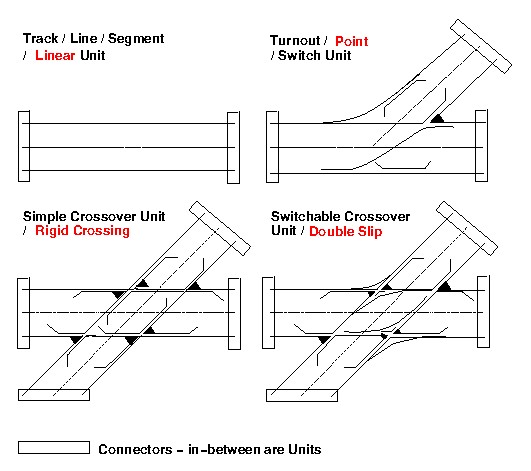
\epsfig{file=rail1.eps,height=\pos{5.4}{11}cm} \ \ 
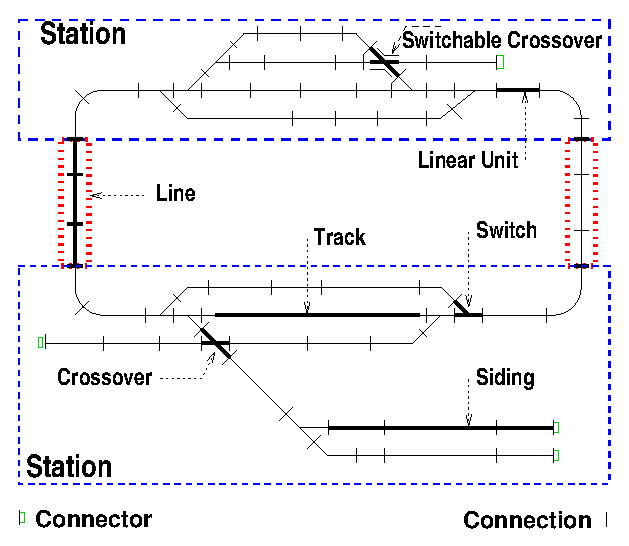
\epsfig{file=rail2.eps,height=\pos{5.4}{9}cm} {[\sort{R}]} 
\caption{{L}eft: Four net units (\textsf{LU, PU, SU, DU}); {R}ight: A railway
  net}\label{fig.railway-net} 
\end{center}
\end{figure}

\mnewfoil

\treprikker

\prinmeth{Pedantic Steps of Development}{primer:pedantic}{%
\begynd
\pind This section, i.e., Sect.\,\ref{sec:Parts}, has illustrated \nyl a principle
      of ``small, pedantic'' analysis \& description steps.
\begynd
\pind You could also call it a principle of separation of concerns\dbsquare
\afslut
\afslut}

\label{before:Ontology and Taxonomy}

\pos{}{%%

\mnewfoil

\vfill
\label{lect2:synth}
\vfill\vspace*{10mm}
\centerline{\lilacolor{Day \#{3}: External Qualities, Synthesis (II)}}
\vfill

}%%%%%%%%

\nbbb{Ontology and Taxonomy}\label{Ontology and Taxonomy}

\begynd
\pind We can speak of two kinds of ontologies\ysf{\footnote{Ontology:
    a set of concepts and categories in a subject area or domain that
    shows their properties and the relations between them [\texttt{Internet}].}}: 
\begynd
\pind the general ontologies of domain analysis \& description, cf.\,Fig.\,\vref{onto.fig2}, and
\pind a specific domain's possible endurant ontologies.
\pind We shall here focus on a [``restricted''] concept of
taxonomies.\footnote{Taxonomy:  a scheme of classification,
      especially a hierarchical classification, in which things are
      organized into groups \wiki.}
\afslut
\afslut

\noindent
\mnewfoil
\bookdefn{Domain Taxonomy}{ By a domain taxonomy we shall understand
\begynd
\pind a hierarchical structure, \nyl usually depicted as a(n
      ``upside-down'') tree,
\pind whose ``root'' designates a compound part
\pind and whose ``siblings'' (proper sub-trees) \nyl designate parts or fluids \dbsquare
\afslut} %%%***

\noindent
\begynd
\pind The `restriction' amounts to considering only endurants.
\pind That is, not considering perdurants.
\pind \isatech{Taxonomy}
\afslut



\noindent
\mnewfoil
\monoexample{The Road Transport System Taxonomy}{%
\begynd
\pind Figure\,\vref{rts.ontology} shows a schematised, i.e., the
      \ldots, taxonomy \nyl
      for the \sfsl{Road Transport System} domain \nyl of Example\,\vref{eks:SoaRTSUoD}.
\afslut
}

\pos{\DBfigure{rts-ontology}{\pos{50mm}{70mm}}{A Road Transport System Taxonomy\dbsquare}{rts.ontology}}
{
 \begin{figure}[h]
  \begin{center}
    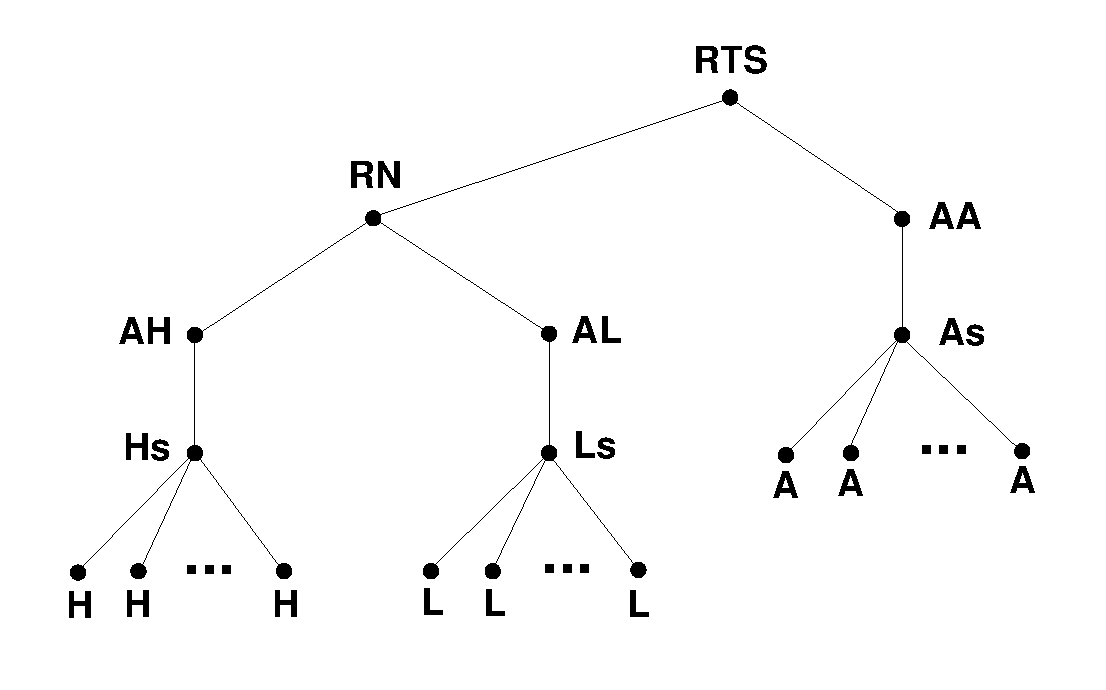
\epsfig{file=rts-ontology.eps,height=\pos{75}{90}mm}
    \caption{A Road Transport System Ontology \dbsquare}\label{rts.ontology}
  \end{center}
\end{figure}
}

\nbbb{``Root'' and ``Sibling'' Parts}\label{Root and Sibling Parts}

\begynd
\pind For compound parts, cf.\,Sect.\,\vref{sec:Compound Parts}, %%%+++
\begynd
\pind we introduce the specific domain taxonomy concepts of ``root'' and ``sibling'' parts.
\pind (We also refer to Fig.\,\vref{rts.ontology}.)
\afslut

\pind When observing, as a human, a compound part\ysf{,} \nyl one may ask the question
\begynd
\pind \sfsl{``a tree \ysf{---} consisting of a specific domain taxonomy node
      labelled, e.g., $X$
\pind and the sub-trees labelled, e.g., $Y_1, Y_2, \ldots, Y_n$ \ysf{---}
\pind does that tree designate one ``indivisible'' part
\pind or does it designate $n+1$ parts\,?''}
\pind We shall, in general, consider the answer to be the latter: $n+1$\,!
\afslut
\afslut

\mnewfoil

\begynd
\pind We shall, in general, consider compound parts to consist of
\begynd
\pind a ``root'' part\ysf{}
\pind and $n$ ``sibling parts and fluids''.
\afslut
\pind What the \ysf{domain modeller} observes
\begynd
\pind appear\ysf{} as one part, ``the whole'',
\pind with $n$ ``embedded'' sub-parts.
\afslut
\pind What the \ysf{domain modeller} is asked to model is
\begynd
\pind $1$, the root part, and
\pind $n$, the sibling\ysf{} parts and fluids.
\afslut
\mnewfoil
\pind The fact that the root part is separately modelled from the sibling parts,
\pind may seem to disappear in this separate modelling ---
\pind but, as You shall see, in the next chapter,
\begynd
\pind their relation: the siblings to ``the whole'', i.e., the root,
\pind will be modelled, specifically through their mereologies,
\pind as will be covered in Sect.\,\ref{chap4.Mereology},
\pind but also through their respective attributes, Sect.\,\ref{chap4.Attributes}.
\afslut
\pind We shall see this non-embbedness of root and sibling parts
\begynd
\pind further accentuated in the modelling of their transcendentally deduced
\pind respective (perdurant) behaviours as distinct concurrent behaviours
\pind in Chapter\,\ref{chap6.tex.1}.
\afslut
\afslut

\label{before:sec:Living Species}

\nbbbb{Living Species}\label{sec:Living Species}

\begynd
\pind \bbcolor{\sfsl{Living Species}} are
\begynd
\pind either \lilacolor{\sfsl{plants}} 
\pind or \lilacolor{\sfsl{animals}}.
\afslut
\pind Among animals we have the \bmcolor{\sfsl{humans}}.
\afslut
\mnewfoil

\nbookdefn{Living Species}{ \label{LivingSpeciesIx}
\begynd
\pind  By a \sfsl{living species} we shall understand \LLLL
\begynd
\pind a solid endurant,
\pind subject to laws of physics, and
\pind additionally subject to \sfsl{causality of
      purpose}. 
\afslut \HHHH
    
\pind Living species
\begynd \LLLL
\pind must have some \sfsl{form they can be developed to reach};
\pind a form they must be \sfsl{causally  determined  to maintain}.
\pind This \sfsl{development and maintenance} must further \nyl engage
      in \sfsl{exchanges of matter with an environment}.
\afslut \HHHH
\pind It must be possible that living species occur in two forms:
\begynd \LLLL
\pind \brcolor{plants}, respectively \brcolor{animals}, 
\pind forms which are characterised by  \nyl \sfsl{development, form and exchange},
\pind which, {additionally}, can be characterised by
\nyl  the \sfsl{ability of purposeful movement}
\ysf{\cite[Kai S{\o}rlander]{kaisorlander1994,kaisorlander1997,kaisorlander2002,kaisorlander2016,kaisorlander2022}}
\dbsquare 
\afslut \HHHH
\afslut
}

\mnewfoil

\newdaprompt{is\_living\_species}{is living species}{$\ell$}{living
  species}{a living species}

\noindent
\isatool{is\_living\_species}

\mnewfoil
\begynd
\pind It is appropriate here to mention \sort{Carl Linnaeus} (1707--1778).
\begynd
\pind He was a Swedish botanist, zoologist, and physician 
\pind who formalised, in the form of a binomial nomenclature, 
\pind the modern system of naming organisms. 
\pind He is known as the ``father of modern taxonomy''.
\pind We refer to his \textsf{`Species Plantarum'} \nyl
      \bbcolor{\texttt{gutenberg.org/files/20771/20771-h/20771-h.htm}}. 
\afslut
\afslut

\nbbb{Plants}\label{sec:Plants}

\monoexample{Plants}{\HHHH%
\begynd
\pind Although we have not yet come across domains for which \nyl the need
      to model the living species of plants were needed, \nyl we give
      some examples anyway:
\begynd
\pind grass,
\pind tulip,
\pind rhododendron,
\pind oak tree.
\afslut
\afslut
}
\mnewfoil

\newdaprompt{is\_plant}{is plant}{$\ell$}{a plant}{a plant}

\noindent
\begynd
\pind \isatool{is\_plant}
\pind The predicate \texttt{is\_living\_species($\ell$)} is a
      prerequisite for \texttt{is\_plant($\ell$)}.
\afslut
      

\nbbb{Animals}\label{sec:Animals}

\nbookdefn{Animal}{ We refer to the initial definition of \sfsl{living
    species} above -- while emphasizing the following traits:
\begynd
\pind (i) a \sfsl{form that animals can be developed to reach} and
\pind (ii)  \sfsl{causally  determined  to  maintain} through
\pind (iii) \sfsl{development and maintenance} \nyl in
      an \sfsl{exchange of matter with an environment}, and
\pind (iv) \sfsl{ability \ysfchgii{of } purposeful movement}
\ysf{\cite[Kai S{\o}rlander]{kaisorlander1994,kaisorlander1997,kaisorlander2002,kaisorlander2016,kaisorlander2022}} \eod
\afslut}

\mnewfoil\pos{\vspace*{-4mm}}{}%t
\newdaprompt{is\_animal}{is animal}{$\ell$}{an animal}{an animal}

\noindent
\begynd
\pind \isatool{is\_animal}
\pind The predicate \texttt{is\_living\_species($\ell$)} is a
      prerequisite for \texttt{is\_animal($\ell$)}.
\pind We distinguish, motivated by \cite[Kai
      S{\o}rlander]{kaisorlander1994,kaisorlander1997,kaisorlander2002,kaisorlander2016,kaisorlander2022},
      between 
\begynd
\pind humans and
\pind other.
\afslut
\afslut

\nbb{Humans}\label{sec:Humans}

\nbookdefn{Human}{
\begynd
\pind A \sfsl{human} (a \sfsl{person}) is an \sfsl{animal}, \nyl
      cf.\,Definition\,\vref{def:Animal},  \nyl with the additional
      properties of having 
\begynd
\pind \sfsl{language},
\pind being \sfsl{conscious} of \sfsl{having knowledge} (of its own
      situation), and
\pind \sfsl{responsibility} \cite[Kai
S{\o}rlander]{kaisorlander1994,kaisorlander1997,kaisorlander2002,kaisorlander2016,kaisorlander2022}
\dbsquare
\afslut
\afslut}

\mnewfoil\pos{\vspace*{-4mm}}{}%t%

\HHHH
\newdaprompt{is\_human}{is human}{$\ell$}{a human}{a human}%
\noindent\HHHH%
\begynd 
\pind \isatool{is\_human}
\pind The predicate \texttt{is\_animal($\ell$)} is a
      prerequisite for \texttt{is\_human($\ell$)}.
\afslut
\mnewfoil\HHHH

\begynd
\pind We have not, \nyl in our many experimental domain modelling efforts
\begynd
\pind had occasion to model humans;
\pind or rather:
\begynd
\pind we have modelled, for example, automobiles
\begynd
\pind as possessing human qualities, 
\pind i.e., ``subsuming humans''.
\afslut
\afslut
\afslut
\mnewfoil
\pind We have found, \nyl  in these experimental domain modelling efforts
\begynd
\pind that we often confer anthropomorphic qualities on artefacts, 
\pind that is, that these artefacts have human characteristics.
\afslut
\pind You, the \pos{readers}{listeners}, are reminded
\begynd
\pind that when some programmers try to explain their programs
\pind they do so using such phrases as
\pind \sfsl{and here the program does ...} so-and-so\,!
\afslut
\afslut

\nbb{Other}\label{sec:Other}

\begynd
\pind We shall skip any treatment of other than human animals\,!
\afslut
\label{chapter1-phy-liv.n}

\treprikker

\noindent
\isaproc{External Quality Analysis \& Description First}

\nbbbbb{Some Observations}\label{Some Observations}

\begynd
\pind Two observations must be made.
 
\begynd
\pind (i) The domain \ysf{modelling} procedures
\begynd
\pind illustrated by
      the analysis functions
\pind  \texttt{de\-term\-ine\_\-Car\-te\-si\-an\_\-parts,
\pind 
      de\-term\-ine\_\-single\_\-sort\_\-part\_set} and
\pind 
      \texttt{de\-term\-ine\_\-al\-tern\-a\-tive\_\-sorts\_\-part\_\-set}
\pind  yield names of
      endurant sorts.
\pind  Some of these names may have already been
      encountered, i.e., discovered.
\pind  That is, the domain \ysf{modeller} must
      carefully consider such possibilities.
\afslut
      
\mnewfoil

\pind (ii) Endurants are \sort{\underline{not}\ recursively definable}\,! 
\begynd
\pind This appears to come as a surprise \nyl to many computer scientists.
\pind Immediately many suggest that ``tree-like'' endurants  \nyl like a river,
\pind or, indeed, a tree, 
\pind should be defined recursively.
\pind But we posit that that is not the case.
\pind A river, for example, has a delta, its ``root'' so-to-speak,
\pind but the sub-trees of a recursively defined river endurant
\pind ha\ysfchg{ve } no such ``deltas''\,! 
\pind Instead we define such
      ``tree-like'' endurants \nyl  as graphs with appropriate
      mereologies \ysf{-- as introduced in the next chapter}.
\afslut
\afslut
\afslut

\label{lect2.label.analysis}


\nbbbbb{States}\label{A Part State}\label{kap3.States.general}\label{lect2.label.synthesis} 

\begynd
\pind In our continued modelling
\begynd
\pind we shall make good use of a concept of states.
\afslut
\afslut

\pos{\vspace*{2mm}}{\vspace*{2cm}}

\bookdefn{State, II}{By a \sfsl{state} we shall understand
\begynd
\pind any collection of one or more parts \dbsquare\
\afslut}
\noindent%
\pos{\psno}{\mnewfoil}%
\begynd%
\pind In Chapter\,\ref{chap4.tex.1} Sect.\,\ref{chap4.Attributes} \nyl
we introduce the notion of \sfsl{attributes.} 
\begynd
\pind Among attributes there are the \sfsl{dynamic attributes}.
\pind They model that internal \ysf{} quality values \nyl  may change dynamically.
\pind So we may wish, on occasion, to `refine' our notion of state
      \nyl to be just those parts which have dynamic attributes.
\afslut
\afslut

\nbbbb{State Calculation}\label{kap3.State Calculation}\label{kap3-gen-state}
\begynd
\pind Given any universe of discourse, \textsf{uod:UoD}, we can
      recursively calculate its ``full'' state, \textsf{calc\_parts({\LBRACE}uod{\RBRACE})}.
\afslut\LLll
\begin{enumerate}\setei
\item \label{uod:state:000} Let \textsf{e} be any endurant. \dbeat{\\}
      Let \textsf{arg\_parts} be the parts to be calculated. \dbeat{\\}
      Let \textsf{res\_parts} be the parts calculated. \dbeat{\\}
      Initialise the \textsf{calc}ulator with
      \textsf{arg\_parts=$\{$uod$\}$} and \textsf{res\_parts=$\{\}$}. \dbeat{\\}
      Calculation stops with \textsf{arg\_parts} empty and
      \textsf{res\_parts} the result.
\item \label{uod:state:010} If  \texttt{is\_Cartesian}(\textsf{e})  
\item \label{uod:state:010a}  then we obtain its
      immediate parts, \textsf{determine\_com\-po\-site\_\-part(e)}
\item \label{uod:state:010b} add them, as a set, to \textsf{arg\_parts}, \textsf{e}
      removed from  \textsf{arg\_parts} and added to
      \textsf{res\_parts} calculating the parts from that.
\item \label{uod:state:012} If 
      \texttt{is\_single\_sort\_part\_set}(\textsf{e}) 
\item \label{uod:state:013} then the parts,
      \textsf{ps}, of the single sort set are determined, 
\item \label{uod:state:014} added to \textsf{arg\_parts} and \textsf{e}
      removed from  \textsf{arg\_parts} and added to
      \textsf{res\_parts} calculating the parts from that.
\item \label{uod:state:016} If
      \texttt{is\_alternative\_sorts\_part\_set}(\textsf{e}) then the
      parts, \textsf{((p1,\_),(p2,\_),...,(pn,\_))}, of 
      the alternative sorts set are determined, added to \textsf{arg\_parts} and \textsf{e}
      removed from  \textsf{arg\_parts} and added to  \textsf{res\_parts} calculating the parts from that.
\savei\end{enumerate}
\pos{\psno}{\mnewfoil}
\noindent
\pos{\doafpr\afindex{calc\_parts}\psno}{\mnewfoil}\pos{}{\normalsize\HHHH\sf}
%\RSLatex
%value
%&\ref{uod:state:000}.&   calc_parts: E-set -> E-set -> E-set
%&\ref{uod:state:000}.&   calc_parts(arg_parts)(res_parts) is
%&\ref{uod:state:000}.&      if arg_parts = {} then res_parts else
%&\ref{uod:state:000}.&      let e :- e isin arg_parts in
%&\ref{uod:state:010}.&      is_Cartesian(e) -> 
%&\ref{uod:state:010a}.&          let ((e1,e2,...,en),_) = observe_Cartesian_part(e) in 
%&\ref{uod:state:010b}.&          calc_parts(arg_parts\{e} union {e1,e2,...,en})(res_parts union {e}) end
%&\ref{uod:state:012}.&      is_single_sort_part_set(e) ->   
%&\ref{uod:state:013}.&          let ps = observe_single_sort_part_set(e) in 
%&\ref{uod:state:014}.&          calc_parts(arg_parts\{e}union ps)(res_parts union {e}) end
%&\ref{uod:state:016}.&      is_alternative_sort_part_set(e) ->    
%&\ref{uod:state:016}.&          let ((p1,_),(p2,_),...,(pn,_)) = observe_alternative_sorts_part_set(e) in 
%&\ref{uod:state:016}.&          calc_parts(arg_parts\{e}union{p1,p2,...,pn})(res_parts union {e}) end
%&\ref{uod:state:000}.&      end end
%\endRSLatex 
\bp
\kw{value}\\
\ref{uod:state:000}.\ \ \ calc\_parts: E\kw{-set} {\RIGHTARROW} E\kw{-set} {\RIGHTARROW} E\kw{-set}\\
\ref{uod:state:000}.\ \ \ calc\_parts(arg\_parts)(res\_parts) {\IS}\\
\ref{uod:state:000}.\ \ \ \ \ \ \kw{if} arg\_parts {\EQ} {\LBRACE}{\RBRACE} \kw{then} res\_parts \kw{else}\\
\ref{uod:state:000}.\ \ \ \ \ \ \kw{let} e {\RDOT} e {\ISIN} arg\_parts \kw{in}\\
\ref{uod:state:010}.\ \ \ \ \ \ is\_Cartesian(e) {\RIGHTARROW} \\
\ref{uod:state:010a}.\ \ \ \ \ \ \ \ \ \ \kw{let} ((e1,e2,{\DOTDOTDOT},en),{\UNDERLINE}) {\EQ} observe\_Cartesian\_part(e) \kw{in} \\
\ref{uod:state:010b}.\ \ \ \ \ \ \ \ \ \ calc\_parts(arg\_parts{\SETMINUS}{\LBRACE}e{\RBRACE} {\UNION} {\LBRACE}e1,e2,{\DOTDOTDOT},en{\RBRACE})(res\_parts {\UNION} {\LBRACE}e{\RBRACE}) \kw{end}\\
\ref{uod:state:012}.\ \ \ \ \ \ is\_single\_sort\_part\_set(e) {\RIGHTARROW}\ \ \ \\
\ref{uod:state:013}.\ \ \ \ \ \ \ \ \ \ \kw{let} ps {\EQ} observe\_single\_sort\_part\_set(e) \kw{in} \\
\ref{uod:state:014}.\ \ \ \ \ \ \ \ \ \ calc\_parts(arg\_parts{\SETMINUS}{\LBRACE}e{\RBRACE}{\UNION} ps)(res\_parts {\UNION} {\LBRACE}e{\RBRACE}) \kw{end}\\
\ref{uod:state:016}.\ \ \ \ \ \ is\_alternative\_sort\_part\_set(e) {\RIGHTARROW}\ \ \ \ \\
\ref{uod:state:016}.\ \ \ \ \ \ \ \ \ \ \kw{let} ((p1,{\UNDERLINE}),(p2,{\UNDERLINE}),{\DOTDOTDOT},(pn,{\UNDERLINE})) {\EQ} observe\_alternative\_sorts\_part\_set(e) \kw{in} \\
\ref{uod:state:016}.\ \ \ \ \ \ \ \ \ \ calc\_parts(arg\_parts{\SETMINUS}{\LBRACE}e{\RBRACE}{\UNION}{\LBRACE}p1,p2,{\DOTDOTDOT},pn{\RBRACE})(res\_parts {\UNION} {\LBRACE}e{\RBRACE}) \kw{end}\\
\ref{uod:state:000}.\ \ \ \ \ \ \kw{end} \kw{end}
\ep
\pos{\rm}{}

\noindent
\isatool{calc\_parts}

\pos{\psno}{\mnewfoil}

\prinmeth{Domain State}{meth:domain-state}{%
\begynd
\pind We have found, once all the state components, \nyl i.e.,
      the endurant parts, \nyl have had their external qualities
      analysed, that
\begynd
\pind it is then expedient to define the domain state.
\pind It can then be the basis for several concepts 
\pind of internal qualities.
\afslut
\afslut}

\pos{\psno}{\mnewfoil}
\monoexample{Constants and States}{
\begin{enumerate}\setei
\item \label{srares-000} Let there be given a universe of discourse,
                         $rts$ (\ysfchg{Road Transport System}). \nyl The set $\{rts\}$ is an example of a state.
\savei\end{enumerate}
\noindent From that state we can calculate other states.

\begin{enumerate}\setei
\item \label{srares-020} The set of all hubs, $hs$. \vidxi{$hs$}{srares-020} 
\item \label{srares-030} The set of all links, $ls$. \vidxi{$ls$}{srares-030} 
\item \label{srares-040} The set of all hubs and links, $hls$. \vidxi{$hls$}{srares-040} 
\item \label{srares-080} The set of all automobiles, $as$. \vidxi{$as$}{srares-080} 
\item \label{srares-090} The set of all parts, $ps$.\vidxi{$ps$}{srares-090} 
\savei\end{enumerate}
\pos{\psno}{\mnewfoil}\ysfchgii{
%\RSLatex
%value
%&\ref{srares-000}&   &$rts$&:UoD
%&\ref{srares-020}&   &$hs$&:H-set  is obs_sH(obs_SH(obs_RN(&$rts$&)))
%&\ref{srares-030}&   &$ls$&:L-set is obs_sL(obs_SL(obs_RN(&$rts$&)))
%&\ref{srares-040}&   &$hls$&:(H|L)-set is &$hs$& union &$ls$&  
%&\ref{srares-080}&   &$as$&:A-set is obs_As(obs_AA(obs_RN(&$rts$&)))
%&\ref{srares-090}&   &$ps$&:(&\ysfchgii{UoD}&|H|L|A)-set is &$rts$& union &$hls$& union &$as$  \eod&
%\endRSLatex    
\bp
\kw{value}\\
\ref{srares-000}\ \ \ $rts$:UoD\\
\ref{srares-020}\ \ \ $hs$:H\kw{-set}\ \ {\IS} obs\_sH(obs\_SH(obs\_RN($rts$)))\\
\ref{srares-030}\ \ \ $ls$:L\kw{-set} {\IS} obs\_sL(obs\_SL(obs\_RN($rts$)))\\
\ref{srares-040}\ \ \ $hls$:(H{\BAR}L)\kw{-set} {\IS} $hs$ {\UNION} $ls$\ \ \\
\ref{srares-080}\ \ \ $as$:A\kw{-set} {\IS} obs\_As(obs\_AA(obs\_RN($rts$)))\\
\ref{srares-090}\ \ \ $ps$:({UoD}{\BAR}H{\BAR}L{\BAR}A)\kw{-set} {\IS} $rts$ {\UNION} $hls$ {\UNION} $as$  \eod
\ep
}}\eysf

\nbbbb{Updateable States}\label{kap3.States.specific}

\begynd
\pind We shall, in Sect.\,\ref{chap4.Attributes}, introduce the notion of parts,
\begynd
\pind having dynamic attributes,
\pind that is, having internal qualities that may change.
\afslut
\pind To cope with the modelling, 
\pind in particular of so-called \sfsl{monitor-able} attributes,
\pind we present the \sfsl{state} as a global variable:
\afslut


%\RSLatex
%variable `sigma := calc_parts({uod})
%\endRSLatex 
\bp
\kw{variable} $\sigma$ :{\EQ} calc\_parts({\LBRACE}uod{\RBRACE})
\ep


\nbbbbb{An External Analysis and Description Procedure}\label{External Analysis and Description Procedure}

\begynd
\pind We have covered 
\begynd
\pind the individual analysis and description steps
\pind of our approach to the external qualities modelling 
\pind of domain endurants. 
\afslut
\pind We now suggest
\begynd 
\pind a `formal' description of the process
\pind of linking all these analysis and description steps.
\afslut
\afslut

\nbbbb{An Analysis \& Description State}\label{A Description State}\label{ADomainDiscoveryNoticeBoard}

\begynd
\pind Common to all the discovery processes is an idea of a
      \sfsl{notice board}. 
\pind A notice board, at any time in the development of a domain
      description,  is a repository of the analysis and description process. 
\pind We suggest to model the notice board in terms of \ysf{four} global
      variables.
\begynd
\pind The \bbcolor{\textsf{new}} variable holds the \bmcolor{parts} yet to be described;
\pind the \bbcolor{\textsf{ans}} variable holds the \bmcolor{sort
      name\ysfchg{s } of parts} that have so far been
      described;
\pind the \bbcolor{\textsf{gen}} variable holds the \bmcolor{parts} that have so far been
      described; and
\pind the \bbcolor{\textsf{txt}} variable holds the \bmcolor{\rsltxt} so far generated.
\begynd
\pind We model  the \bbcolor{\textsf{txt}} variable as a  map 
\pind from endurant identifier names to \bmcolor{\rsltxt}.
\afslut
\afslut
\afslut\HHHH
\pos{\psno}{\mnewfoil}

\vspace*{2mm}

\boiteepaisseavecuntitre{Discovery Schema 0: The Notice Board}
\label{DiscoverySchema0}\label{A Domain Discovery Notice Board}
%\RSLatex
%variable
%   new := {uod} ,
%   asn := { &\bq& UoD &\eq& }
%   gen := {} ,
%   txt:&\rsltxt&  := [ uid_UoD(uod) +> <.&\bq&type UoD&\eq&.> ]
%\endRSLatex
\bp
\kw{variable}\\
\>\ new :{\EQ} {\LBRACE}uod{\RBRACE} ,\\
\>\ asn :{\EQ} {\LBRACE} \bq UoD \eq {\RBRACE}\\
\>\ gen :{\EQ} {\LBRACE}{\RBRACE} ,\\
\>\ txt:\rsltxt\ \ :{\EQ} {\LBRACKET} uid\_UoD(uod) {\MAPSTO} {\LANGLE}\bq\kw{type} UoD\eq{\RANGLE} {\RBRACKET}
\ep
\endboiteepaisseavecuntitre\pos{\normalsize}{\HHHH}\rm


\nbbbb{A Domain Discovery Procedure, I}\label{The Procedure}\label{A Domain Discovery Process, I}
 
\begynd
\pind The \textsf{discover\_sorts} pseudo program
\begynd
\pind suggests a systematic way of proceeding
\pind through analysis, manifested by the \textsf{is\_$\cdots$} predicates,
\pind to ({\RIGHTARROW}) description.
\afslut
\afslut

\begynd
\pind Some comments are in order.
\begynd
\pind The \textsf{e-set$_a$}$\sqcupplus$\textsf{e-set$_b$} expression
\pind yields a set of endurants that are either in \textsf{e-set$_a$},
      or in \textsf{e-set$_a$}, or in both,
\pind but such that two endurants, \textsf{e$_x$} and \textsf{e$_y$}
\pind which are of the same endurant\ysfchg{ } type, say \textsf{E}, 
\pind and are in respective sets is only represented once in the
      result\ysfchg{. }\dbeat{ 
\pind that is, if they are type-wise the same, but value-wise different
\pind they will only be included once in the result.}
\afslut
                                \pos{\psno}{\mnewfoil}\HHHH

\pind As this is the first time \rsltxt\ is put on the notice board \nyl we express this as:
\begin{itemize}
\item \textsf{txt :{\EQ} txt {\UNION} {\LBRACKET}type\_name(v) {\MAPSTO} {\LANGLE}\rsltxt{\RANGLE}{\RBRACKET}}
\end{itemize}
\pind Subsequent insertion of \rsltxt\ \nyl for internal quality
descriptions and perdurants  \nyl is then concatenated to the end of
previously uploaded \rsltxt.
\afslut

\pos{\psno\vspace*{4mm}}{\mnewfoil \vspace*{-4mm}}

\boiteepaisseavecuntitre{\LLll \ysf{Discovery Schema 1: An
    External Qualities Domain Modelling} Process} \label{DiscoverySchema1}
\LLll
  
\pos{\footnotesize\small\normalsize}{\Large}\label{discover-sorts}
%\RSLatex
%value
% discover_sorts: Unit -> Unit
% discover_sorts() is while new ~= {} do 
%   let v :- v isin new in (new := new \ {v} || gen := gen union {v} || ans := ans \ {type_of(v)}) ;
%   is_atomic(v) -> skip ,
%   is_compound(v) ->
%    is_Cartesian(v) ->
%     let ((e1,...,en),(&$\eta$E1,...,$\eta$En&))=determine_Cartesian_part_sorts(v) in&\afindex{determine\_Cartesian\_part\_sorts}&
%     (ans := ans union {&$\eta$E1,...,$\eta$En&} || new := new &$\sqcupplus$& {e1,...,en}  
%      || txt := txt union [type_name(v) +> <.describe_Cartesian_part_sorts(v).>]) end,&\dpindex{describe\_Cartesian\_part\_sorts}& 
%    is_part_set(v) ->
%     let ({p1,...,pn},&$\eta$P&)=determine_part_set_sort(v) in&\afindex{determine\_part\_set\_sort}&
%     (ans := ans union {&$\eta$P&} || new := new &$\sqcupplus$& {p1,...,pn} ||
%      txt := txt union [type_name(v) +> describe_part_set_sort(v)]) end,&\dpindex{describe\_part\_set\_sort}& 
%  end end
%\endRSLatex
\bp
\kw{value}\\
 discover\_sorts: \kw{Unit} {\RIGHTARROW} \kw{Unit}\\
 discover\_sorts() {\IS} \kw{while} new {\NOTEQ} {\LBRACE}{\RBRACE} \kw{do} \\
\>\ \kw{let} v {\RDOT} v {\ISIN} new \kw{in} (new :{\EQ} new {\SETMINUS} {\LBRACE}v{\RBRACE} {\PARL} gen :{\EQ} gen {\UNION} {\LBRACE}v{\RBRACE} {\PARL} ans :{\EQ} ans {\SETMINUS} {\LBRACE}type\_of(v){\RBRACE}) ;\\
\>\ is\_atomic(v) {\RIGHTARROW} \kw{skip} ,\\
\>\ is\_compound(v) {\RIGHTARROW}\\
\>\>is\_Cartesian(v) {\RIGHTARROW}\\
\>\>\ \kw{let} ((e1,{\DOTDOTDOT},en),($\eta$E1,...,$\eta$En)){\EQ}determine\_Cartesian\_part\_sorts(v) \kw{in}\afindex{determine\_Cartesian\_part\_sorts}\\
\>\>\ (ans :{\EQ} ans {\UNION} {\LBRACE}$\eta$E1,...,$\eta$En{\RBRACE} {\PARL} new :{\EQ} new $\sqcupplus$ {\LBRACE}e1,{\DOTDOTDOT},en{\RBRACE}\ \ \\
\>\>\>{\PARL} txt :{\EQ} txt {\UNION} {\LBRACKET}type\_name(v) {\MAPSTO} {\LANGLE}describe\_Cartesian\_part\_sorts(v){\RANGLE}{\RBRACKET}) \kw{end},\dpindex{describe\_Cartesian\_part\_sorts} \\
\>\>is\_part\_set(v) {\RIGHTARROW}\\
\>\>\ \kw{let} ({\LBRACE}p1,{\DOTDOTDOT},pn{\RBRACE},$\eta$P){\EQ}determine\_part\_set\_sort(v) \kw{in}\afindex{determine\_part\_set\_sort}\\
\>\>\ (ans :{\EQ} ans {\UNION} {\LBRACE}$\eta$P{\RBRACE} {\PARL} new :{\EQ} new $\sqcupplus$ {\LBRACE}p1,{\DOTDOTDOT},pn{\RBRACE} {\PARL}\\
\>\>\>txt :{\EQ} txt {\UNION} {\LBRACKET}type\_name(v) {\MAPSTO} describe\_part\_set\_sort(v){\RBRACKET}) \kw{end},\dpindex{describe\_part\_set\_sort} \\
\>\kw{end} \kw{end}
\ep
\endboiteepaisseavecuntitre\pos{\normalsize}{\HHHH}\rm
\noindent
\pos{\psno}{\mnewfoil}%%%

\pos{\noindent
\isaproc{discover\_sorts}}{}
  
\nbbbbb{Summary}\label{sec:extq.Summary}\label{X:Summary}

\begynd
\pind We briefly summarise the main findings of this \pos{chapter}{lecture}.
\pind These are the main 
\begynd
\pind analysis predicates and functions\ysfchg{, }
      and
\pind  the main description functions.
\afslut
\pind These, to remind the \pos{reader}{student}, are
\begynd
\pind \ysfchg{(i) } the \sfsl{analysis}, the \texttt{is\_$\cdots$}, \sfsl{predicates},
\pind \ysfchg{(ii) }  the \sfsl{analysis}, the \texttt{determine\_$\cdots$},
      \sfsl{functions}, 
\pind \ysfchg{(iii) }  the \sfsl{state calculation} function, 
\pind \ysfchg{(iv) }  the \sfsl{description} functions, and
\pind \ysfchg{(v) }  the \sfsl{domain discovery} procedure.
\afslut
\afslut
\mnewfoil

\pos{
\begynd
\pind They are summarised in this table:
\afslut

\pos{\boiteepaisseavecuntitre{\brcolor{External Qualities Predicates and
Functions: Method Tools}}
\label{functions-table-1}
\begin{minipage}[h]{5.5cm}\sf\small\sf
\begin{quote}
\begin{itemize}
\item \sort{Analysis Predicates:} These are the \texttt{is\_$\cdots$}
  functions. The domain scientist cum engineer, i.e., the domain
  analyser cum describer, applies this to entities being observed in
  the domain. The answer is a truth value. Dependent on the truth value
  that person then goes on to apply, again informally, either a
  subsequent predicate, or some function.
\item \sort{Analysis Functions:} These are the
  \texttt{determine\_$\cdots$} functions. They apply, respectively, to
  parts satisfying respective predicates.
\item \sort{State Calculation:} The state calculation function is
  given generally. The domain analyser cum describer must define this
  function for each domain studied.
\item \sort{Description Functions:} These calculation functions, in a
  sense, are the main ``results'' of this chapter.
\item \sort{Domain Discovery:} The procedure here being described,
  informally, guides the domain analyser cum describer to do the job\,!
\end{itemize}\normalsize
\end{quote}
\end{minipage}
\begin{minipage}[h]{5mm} \ \
\end{minipage}
\begin{minipage}[h]{7cm}\small\sf
\qbtabular\\
%                     
%%%%%%%%%%%%%%%%%%%%%%%%%%%%%%%%%%%%%%%%%%%%%%%%%%%%%%%%%%%%%%%%%%%%%%%
%%%% Released for translation 22 April 2023  %%%%%%%%%%%%%%%%%%%%%%%%%%
%%%%%%%%%%%%%%%%%%%%%%%%%%%%%%%%%%%%%%%%%%%%%%%%%%%%%%%%%%%%%%%%%%%%%%%         %
& \ \ \ \brcolor{Analysis Predicates} & \\
\plineo{dap:is-entity}{is\_entity}{isentity}\\
\plineo{dap:is-endurant}{is\_endurant}{isendurant}\\
\plineo{dap:is-perdurant}{is\_perdurant}{isperdurant}\\
\plineo{dap:is solid}{is\_solid}{issolid}\\
\plineo{dap:is fluid}{is\_fluid}{isfluid}\\
\plineo{dap:is physical part}{is\_part}{isphysicalpart}\\
\plineo{dap:is atomic part}{is\_atomic}{isatomicpart}\\
\plineo{dap:is compound part}{is\_compound}{iscompoundpart}\\
\plineo{dap:is-cartesian}{is\_Cartesian}{iscartesian}\\
\plineo{dap:is-single-sort-set}{is\_part\_set\ysfchg{\_sort}}{issinglesortset}\\
\plineo{dap:is living species}{is\_living\_species}{a living species}\\
\plineo{dap:is plant}{is\_plant}{a plant}\\
\plineo{dap:is animal}{is\_animal}{an animal}\\
\plineo{dap:is human}{is\_human}{a human}\\
& \ \ \ \brcolor{Analysis Functions} & \\
\plineo{dap:analyse-cp}{determine\_Cartesian\_part\_sorts}{determineCartesian}\\
\plineo{dap:determine-single-sort-part-set}{determine\_part\_set\_sort}{DsSpS}\\
& \ \ \ \brcolor{State Calculation} & \\
\pline{calc\_parts}{uod:state:000}\\
& \ \ \ \brcolor{Description Functions} & \\
\plineo{ddp:UoD}{describe\_Universe\_of\_Discourse}{DS1}\\
\plineo{ddp:calc-Cartesian-parts}{describe\_Cartesian\_part\_sorts}{DS2}\\
\plineo{ddp:calc-single-sort-part-set-sorts}{describe\_part\_set\_sort}{DS3}\\
& \ \ \ \brcolor{Domain Discovery} & \\
\pline{discover\_sorts}{discover-sorts}\\

\qetabular\normalsize
\end{minipage}
\endboiteepaisseavecuntitre
%%  LocalWords:  analyser
}{\normalsize\large\large%\vspace*{-15mm}
\qbtabular\\
\pos{}{\large}%                     
%%%%%%%%%%%%%%%%%%%%%%%%%%%%%%%%%%%%%%%%%%%%%%%%%%%%%%%%%%%%%%%%%%%%%%%
%%%% Released for translation 22 April 2023  %%%%%%%%%%%%%%%%%%%%%%%%%%
%%%%%%%%%%%%%%%%%%%%%%%%%%%%%%%%%%%%%%%%%%%%%%%%%%%%%%%%%%%%%%%%%%%%%%%         %
& \ \ \ \brcolor{Analysis Predicates} & \\
\plineo{dap:is-entity}{is\_entity}{isentity}\\
\plineo{dap:is-endurant}{is\_endurant}{isendurant}\\
\plineo{dap:is-perdurant}{is\_perdurant}{isperdurant}\\
\plineo{dap:is solid}{is\_solid}{issolid}\\
\plineo{dap:is fluid}{is\_fluid}{isfluid}\\
\plineo{dap:is physical part}{is\_part}{isphysicalpart}\\
\plineo{dap:is atomic part}{is\_atomic}{isatomicpart}\\
\plineo{dap:is compound part}{is\_compound}{iscompoundpart}\\
\plineo{dap:is-cartesian}{is\_Cartesian}{iscartesian}\\
\plineo{dap:is-single-sort-set}{is\_part\_set\ysfchg{\_sort}}{issinglesortset}\\
\plineo{dap:is living species}{is\_living\_species}{a living species}\\
\plineo{dap:is plant}{is\_plant}{a plant}\\
\plineo{dap:is animal}{is\_animal}{an animal}\\
\plineo{dap:is human}{is\_human}{a human}\\
& \ \ \ \brcolor{Analysis Functions} & \\
\plineo{dap:analyse-cp}{determine\_Cartesian\_part\_sorts}{determineCartesian}\\
\plineo{dap:determine-single-sort-part-set}{determine\_part\_set\_sort}{DsSpS}\\
& \ \ \ \brcolor{State Calculation} & \\
\pline{calc\_parts}{uod:state:000}\\
& \ \ \ \brcolor{Description Functions} & \\
\plineo{ddp:UoD}{describe\_Universe\_of\_Discourse}{DS1}\\
\plineo{ddp:calc-Cartesian-parts}{describe\_Cartesian\_part\_sorts}{DS2}\\
\plineo{ddp:calc-single-sort-part-set-sorts}{describe\_part\_set\_sort}{DS3}\\
& \ \ \ \brcolor{Domain Discovery} & \\
\pline{discover\_sorts}{discover-sorts}\\

\qetabular\HHHH}
}{}

\mnewfoil

\treprikker

\noindent
\begynd
\pind Please consider Fig.\,\ref{onto.fig2} [\pos{Page}{Slide}\,\pageref{onto.fig2}].
\begynd
\pind This \pos{chapter}{lecture} has covered the tree-like structure
      \nyl to the left in  Fig.\,\ref{onto.fig2}.
\pind The next \pos{chapter covers}{lectures cover} the horisontal and
      vertical lines, 
      \nyl also to the left in Fig.\,\ref{onto.fig2}.
\afslut
\afslut
\label{primer-extq.n}

%%  LocalWords:  Endurants analysed analyser endurant RTS priori et
%%  LocalWords:  formalise endurants perdurants perdurant verbed eks
%%  LocalWords:  cetera geo plasmatic compartmentalise fn analyse RSL
%%  LocalWords:  characterisation artefactual atomism analysing wrt
%%  LocalWords:  modelling cartesian po cp Ei Cartesians calc eind SL
%%  LocalWords:  Formalisation Disjointness typenames UoD pts ved un
%%  LocalWords:  cluding ps Pn pn le Hs al tive disjointness NUs SU
%%  LocalWords:  LinU PntU SwiU DblU TerU eft ight characterised www
%%  LocalWords:  formalised gu modelled artefacts txt uod asn uid rts
%%  LocalWords:  ontologies taxonomical schematised labelled arg hs
%%  LocalWords:  Initialise ulator srares hls bcs bs sH sL BCs SBC FV
%%  LocalWords:  bc UoB ddp isphysicalpart isatomicpart iscartesian
%%  LocalWords:  iscompoundpart doaf Defn mereologies embbedness UoDs
%%  LocalWords:  behaviours Plantarum summarise indsnaevring filosofi
%%  LocalWords:  Kai rlander sep Artifactual de ine te si summarised
%%  LocalWords:  horisontal sortness modeller SoaRTSUoD VDM pdefind
%%  LocalWords:  characterises Updateable pconind omments ve
     % External Qualities
 



%%%%%%%%%%%%%%%%%%%%%%%%%%%%%%%%%%%%%%%%%%%%%%%%%%%%%%%%%%%%%%%%%%%%%%%
%%%% Re-released for translation 22 June 2023  %%%%%%%%%%%%%%%%%%%%%%%%%%
%%%%%%%%%%%%%%%%%%%%%%%%%%%%%%%%%%%%%%%%%%%%%%%%%%%%%%%%%%%%%%%%%%%%%%%


\nbbbbbb{Endurants: Internal and Universal Domain Qualities}\label{chap4.tex.1}
\pos{\minitoc}{}

\vspace*{2mm}

\noindent
\begynd
\pind Please consider Fig.\,\vref{onto.fig2}.
\begynd
\pind The previous chapter covered the tree-like structure to the left in  Fig.\,\ref{onto.fig2}.
\pind This chapter covers the \ysf{vertical and  hori\ysfchg{z}ontal} lines, also
      to the left\ysf{,} in Fig.\,\ref{onto.fig2}.
\afslut
\afslut

\treprikker

\mnewfoil

\HHHH
\noindent 
\begynd
\pind In this chapter we introduce 
\begynd 
\pind the concepts of internal qualities of endurants and \ysf{some} universal
      qualities of domains, 
\pind and cover, first, the analysis and description of internal qualities:
\LLLL\HHHH
\begynd
\pind \bbcolor{unique identifiers} (Sect.\,\vref{chap4.Unique Identification}),
\pind \bbcolor{mereologies} (Sect.\,\vref{chap4.Mereology}) and
\pind \bbcolor{attributes} (Sect.\,\vref{chap4.Attributes})\ysf{.}
\afslut
\mnewfoil
\pind There is, additionally, three \sort{universal qualities:}
\begynd
\pind \bbcolor{space}, \bbcolor{time} (Sect.\,\vref{space and time}) and
\pind \bbcolor{intentionality} (Sect.\,\vref{chap4.Intentional Pull}), where
\begynd
\pind \sfsl{intentionality} is  ``something'' that expresses
\pind intention, design idea, purpose of artefacts -- 
\pind well, some would say, also of natural endurants.
\afslut
\afslut
\afslut

\mnewfoil

\pind As it turns out\pos{\footnote{You, the first time reader cannot
    know this, i.e., the ``turns out''. Once we have developed and
    presented the material of this chapter, then you can see it;
    clearly\,!}}{\stepcounter{footnote}}, 
\begynd
\pind to analyse and describe mereology
\pind we need to first analyse and describe unique identifiers;
\afslut
and
\begynd
\pind to analyse and describe attributes
\pind we need to first analyse and describe mereologies.
\afslut
\mnewfoil
\pind Hence:
\afslut

\procmeth{\nyl{Sequential Analysis \& Description of} \nyl Internal
          Qualities}{methstp:saadoiq}{%
\begynd
\pind We advise that the \ysf{domain modeller:}
\begin{itemize}
\item  \sort{first} analyse \& describe  \nyl \bbcolor{unique identification} of all endurant sorts;
\item  \sort{then}  analyse \& describe \nyl \bbcolor{mereologies} of all endurant sorts;
\item  \ysf{\sort{then}} analyse \& describe \nyl \bbcolor{attributes}
  of all endurant sorts; and,
\item  \ysf{\sort{finally}, to analyse \& describe \nyl \bbcolor{intentionality}.} 
\end{itemize}
\afslut}

\bookdefn{Description, II}{ %
\begynd
\pind By a \sort{description} \index{pdefind}{description!internal qualities} of the internal
      qualities of a domain
\begynd
\pind we mean pairs of informal, narrative, and formal text
\pind which characterises the
\begynd
\pind unique identifiers,
\pind mereologies,
\pind attributes, and possible
\pind intentional pulls
\afslut
\pind of manifest parts (fluids and living species) \dbsquare
\afslut
\afslut
}

\noindent
\begynd
\pind This chapter explains what is meant by 
\begynd
\pind \sfsl{unique identifier}, \index{pconind}{unique identifier} 
\pind \sfsl{mereology},  \index{pconind}{mereology}
\pind \sfsl{attribute} and \index{pconind}{attribute}
\pind \sfsl{intentional pull}. \index{pconind}{intentional pull}
\afslut
\afslut
\mnewfoil

\nbbbbb{Internal Qualities}\label{chap4.Internal Qualities}

\noindent
\inthis{\nyl internal qualities}{the properties
of the entities \nyl to which we ascribe internal qualities.}{}

\nbbbb{General Characterisation}

\begynd%
\pind {External qualities} of endurants of a manifest domain
\begynd
\pind are, in a simplifying sense, those we can
\begynd
\pind see and
\pind touch.
\afslut
\pind They, so to speak, take form.
\afslut
\afslut
\pos{\psno}{\mnewfoil}%

\begynd%
\pind \bbcolor{Internal qualities} of endurants of a manifest domain
\begynd
\pind are, in a less simplifying sense, those which
\begynd
\pind we may not be able to see or ``feel'' \nyl when touching an endurant,
\pind but they can, as we now `mandate' them,
\begynd
\pind be reasoned about, \nyl as for \brcolor{unique identifiers} \nyl and \brcolor{mereologies},
\afslut or
\pind be measured by some \sort{physical/chemical} means,
\pind or be ``spoken of'' by \sort{intentional deduction}, and
\begynd
\pind be reasoned about,
\afslut
\pind as we do when we \brcolor{attribute} properties to endurants.
\afslut
\afslut
\afslut

\nbbbb{Manifest Parts versus Structures}

\begynd
\pind In \cite{BjornerMonograph2020} we covered a notion of \sfsl{`structures'}.
\begynd
\pind In this primer we shall treat \nyl  the concept of `structures'
differently\ysfchg{. }
\pind We do so by distinguishing between
\begynd
\pind manifest parts 
\pind and structures.
\afslut
\afslut
\afslut

\nbbb{Definitions}

\bookdefn{Manifest Part:}{ By a manifest part\index{pdefind}{manifest
      part}\index{pdefind}{part!manifest} we shall understand
\begynd
\pind a part which `manifests' itself 
\begynd
\pind either in a physical, visible
      manner, ``occupying'' \nyl an $\mathbb{AREA}$ or \nyl a $\mathbb{VOLUME}$
      and \nyl a $\mathbb{POSITION}$  \nyl in  $\mathbb{SPACE}$, 
\pind or in a conceptual manner \nyl  forms an organisation in Your
      mind\,!\dbsquare\ \
\afslut 
\pind As we have already revealed,   
\pind endurant parts can be \nyl transcendentally
      deduced into perdurant behaviours   
\pind -- with manifest parts indeed being so.
\afslut}

\mnewfoil
\bookdefn{Structure}{ By a structure\index{pdefind}{structure} we shall
      understand
\begynd
\pind an endurant concept that allows \nyl  the domain \ysf{modeller}
\begynd
\pind to rationally decompose \nyl  a domain analysis and/or its description 
\pind into manageable, logically relevant sections,  
\pind but where these abstract endurants \nyl  are not further reflected
      upon \nyl  in the domain analysis and description.
\afslut
\pind Structures are therefore \nyl  not  transcendentally
      deduced into perdurant behaviours.
\afslut}

\nbbb{Analysis Predicates}

\daprompt{is\_manifest}{is-manifest}{\label{is manifest pt}%
\begynd
\pind The method provides the \dap:
\begin{itemize}
\item \bcolor{\texttt{is\_manifest}}
     \doanpr\pos{\apindex{is\_manifest}}{}
      -- where 
      \texttt{is\_manifest($p$)} \nyl  holds if $p$ is to be considered manifest\eoap
\end{itemize}
\afslut
}
\daprompt{is\_structure}{is-structure}{\label{is structure pt}%
\begynd
\pind The method provides the \dap:
\begin{itemize}
\item \bcolor{\texttt{is\_structure}}
     \doanpr\apindex{is\_structure}
      -- where 
      \texttt{is\_structure($p$)} \nyl  holds if $p$ is to be considered a structure\eoap
\end{itemize}
\afslut
}

\noindent
\begynd
\pind The obvious holds:
      \bcolor{\texttt{is\_manifest}(p)}\,{\IS}\,\ysfchgii{\SIM}\,\bcolor{\texttt{is\_structure}(p)}. 
\afslut

\nbbb{Examples}\LLLL
\monoexample{Manifest Parts and Structures}{\LLLL
  We refer to Example\,\vref{A Road Transport System Domain: Cartesians}: the Road
     Transport System.
\begynd
\pind We shall consider all atomic parts: hubs, links and automobiles
      as being manifest. \nyl (They are physical, visible and in $\mathbb{SPACE}$.)
\pind We shall consider road nets and aggregates of automobiles as
      being manifest.
\begynd 
\pind Road nets are physical, visible and in $\mathbb{SPACE}$.
\pind Aggregates of automobiles are here considered conceptual.
\pind The road net manifest part, 
\begynd 
\pind apart from it\ysf{s} aggregates of hubs and links, 
\pind can be thought of as ``representing'' a \sfsl{Department of Roads}\footnotemark.
\afslut 
\pind The automobile aggregate 
\begynd
\pind apart from its automobiles,
\pind can be thought of as ``representing'' a \sfsl{Department of Vehicles}\footnotemark.
\afslut
\pind We shall\ysf{, at present,} consider hub and link aggregates and
hub and link set\ysf{s} as structures \eod
\afslut
\afslut}
\addtocounter{footnote}{-1}
\footnotetext{\LLLL -- of some country, state, province, city or other.}
\addtocounter{footnote}{1}
\footnotetext{\LLLL See above footnote.}

\nbbb{Modelling Consequence}\HHHH

\begynd
\pind \ysf{} If a part is considered manifest \nyl then we shall endow that part \nyl with all
      three kinds of internal qualities.
\pind If a part is considered a structure \nyl then we shall \sort{not}
      endow that part \nyl with any 
      of \ysfchg{the } three kinds of internal qualities.
\afslut

\nbbbbb{Unique Identification}\label{chap4.Unique Identification}

\noindent
\begynd
\pind The concept of parts having unique identifiability,
\begynd
\pind that is, that two parts, 
\pind if they are the same,
\pind have the same unique identifier,
\pind and if they are not the same,
\pind then they have distinct identifiers,
\pind that concept is fundamental to our being able \nyl
      to analyse and describe internal qualities of endurants.
\afslut
\pind So we are left with the issue of `identity'\,!
\pos{\pind \ysf{(We refer to Sect.\,\vref{IdentityKS}.)}}{}
\afslut

\mnewfoil

\bookdefn{Uniqueness}{ %
\begynd
\pind By uniqueness of parts we shall mean
\begynd
\pind that any two spatially distinct parts
\pind are two unique parts --
\pind cannot be confused \dbsquare\
\afslut
\afslut
}

\bookdefn{Unique Identifier}{ %
\begynd
\pind By a unique identifier we shall mean
\begynd
\pind anything that can be used to distinguish
\pind any one part from any other spatially distinct parts \dbsquare\
\afslut
\afslut
}

\nbbbb{On Uniqueness of Endurants}

\begynd
\pind We therefore introduce the notion of \nyl unique identification of
      part endurants.
\pind We assume
\begynd
\pind (i) that all part endurants, \textsf{e}, of any domain
      \textsf{E}, \nyl have 
      \pcindextermii{unique}{identifier}s, 
\pind (ii) that \pcindextermii{unique}{identifier}s
      (of part endurants \textsf{e:E}) \nyl 
      are \pcindextermii{abstract}{value}s \nyl
      (of the \pcindextermii{unique}{identifier} sort \textsf{UI} of part endurants
      \textsf{e:E}), 
\pind (iii) \ysf{} that distinct part endurant sorts, \textsf{E$_i$} and
      \textsf{E$_j$},\nyl\ have distinctly named
      \pcindextermii{unique}{identifier} sorts, \nyl say \textsf{UI$_i$} and
      \textsf{UI$_j$}\footnote{\LLLL This restriction is not
        necessary, but, for the time \ysfchg{being}, we can assume that it is.}, and 
\pind (iv) that all \textsf{$ui_i$:UI$_i$} and \textsf{$ui_j$:UI$_j$} are
      distinct.
\afslut
\afslut

\pos{\psno}{\mnewfoil}
\typo{\begynd
\pind The names of unique identifier sorts, say \textsf{UI}, \nyl is
      entirely at the discretion of \nyl  the \sfsl{domain \ysf{modeller}}.
      \pind If, for example, the sort name of a part\ \ is \textsf{P}, \nyl
     then it might be expedient to \nyl  name the sort of the unique
     identifiers of its parts \textsf{PI}.
\afslut}

\pos{\psno}{\mnewfoil}

\bgcolor{Representation of Unique Identifiers:}{ %
\begynd
\pind Unique identifiers are abstractions.
\begynd
\pind When we endow two endurants (say of the same sort) \nyl 
      distinct unique identifiers
\pind then we are simply saying that \nyl  these two endurants are distinct.
\pind We are not assuming anything about \nyl how these identifiers
      otherwise come about. 
\afslut%
\afslut%
}
\mnewfoil 
\bgcolor{Identifiability of Endurants:}{
\begynd
\pind From a philosophical point of view, 
\begynd
\pind and with basis in \kaisorfil\pos{, \nyl cf.\,Paragraph \bmcolor{Identity, Difference and
      Relations} (\pos{Page}{Slide}\,\pageref{Identity and Relations})}{}, 
\pind one can rationally argue that there are many endurants,
\pind and that they are unique, and hence uniquely identifiable.
\afslut
\pind From an empirical point of view,
\begynd
\pind and since one may eventually \nyl
      have a software development in mind,
\pind we may wonder how unique identifiablity can be accommodated.
\afslut
\afslut
}

\mnewfoil\HHHH
\begynd
\pind Unique identifiability for solid endurants,
\begynd
\pind even though they may be mobile, 
\pind is straightforward:
\begynd
\pind one can think of many ways  
\pind of ascribing a unique identifier to any part\ysf{.}
\afslut
\afslut
\pind Hence one can think of many such unique identification schemas.
\afslut

\mnewfoil
\begynd
\pind Unique identifiability for fluids may seem a bit more tricky.
\begynd
\pind For this \monograph\ we shall not suggest
\pind to endow fluids with unique identification.
\pind We have simply not experimented with such \nyl
      part-fluids and fluid-parts domains \nyl
      -- not enough -- to suggest so. 
\afslut
\afslut

\nbbbb{Uniqueness Modelling Tools}\label{kap4.Uniqueness Modeling Tools}
 
\begynd
\pind The analysis method offers an
      observer function \textsf{{\uidmo}E} \nyl which when applied to \ysfchg{a }
      part endurant\ysfchg{, } \textsf{e} \ysf{of sort \textsf{E}}, \nyl
      yields the unique identifier,  $ui$:\textsf{EI}, of \textsf{e}.
\afslut
\ddprompt{describe\_unique\_identifier}{observe-unique-identifier}{\label{duid}%%
\begynd
\pind We can therefore apply the \ddp:
\begin{itemize}
\item \bcolor{\texttt{describe\_unique\_identifier}}%
      \dodepr\dpindex{describe\_unique\_identifier}%% 
\end{itemize}
\emmar
\noindent
\pind to endurants \textsf{e:E} 
\begynd
\pind resulting in the analyser writing down
\pind the \ddtu{Unique Identifier Type and Observer} 
\afslut
\afslut
\mnewfoil\bdbrule

{\bgcolor{\bgcolor{\cdlti}\ 
      \texttt{describe\_unique\_identifier(e)}} \sort{Observer}}
      \delati{describe\_unique\_identifier}%
      \ddlt{PartUniqueIdentifier}{dlti}
%\RSLatex
%&\bq\kw{Narration:}&
%   [s]   ... narrative text on unique identifier sort EI ...&\footnotemark&
%   [u]   ... narrative text on unique identifier observer &{\uidmo}&E ...
%   [a]   ... &axiom on& uniqueness &of& unique identifiers ...
%& \kw{Formalisation:}&
%   type
%   [s]   UI
%   value
%   [u]   &{\uidmo}&E: E -> EI&\delaoi{\protect{\uidmo}}\label{uidP}\eq& 
%\endRSLatex 
\bp
\bq\kw{Narration:}\\
\>\ {\LBRACKET}s{\RBRACKET}\ \ \ {\DOTDOTDOT} narrative text on unique identifier sort EI {\DOTDOTDOT}\footnotemark\\
\>\ {\LBRACKET}u{\RBRACKET}\ \ \ {\DOTDOTDOT} narrative text on unique identifier observer {\uidmo}E {\DOTDOTDOT}\\
\>\ {\LBRACKET}a{\RBRACKET}\ \ \ {\DOTDOTDOT} axiom on uniqueness of unique identifiers {\DOTDOTDOT}\\
 \kw{Formalisation:}\\
\>\ \kw{type}\\
\>\ {\LBRACKET}s{\RBRACKET}\ \ \ UI\\
\>\ \kw{value}\\
\>\ {\LBRACKET}u{\RBRACKET}\ \ \ {\uidmo}E: E {\RIGHTARROW} EI\delaoi{\protect{\uidmo}}\label{uidP}\eq 
\ep
\edbrule%\lddemmar
}
\footnotetext{\LLLL\typo{The name, \textsf{EI}, of the unique identifier
  sort is determined, \sfsl{``pulled out of a hat''}, by the domain
  \ysf{modeller}(s), i.e., the person(s) who ``apply'' the
  \texttt{describe\_unique\_identifier(e)} prompt.}}
\noindent
\begynd
\pind \texttt{is\_part(e)} is a prerequisite for \texttt{describe\_unique\_identifier(e)}.
\afslut

\pos{\psno}{\mnewfoil}
\begynd
\pind The unique identifier type name,  \textsf{EI} above, 
\begynd
\pind chosen, of course, by the
      \sfsl{domain \ysf{modeller}}, 
\pind usually properly embodies the
      type name, \textsf{E}, 
\pind of the endurant being analysed and
      mereology-described.
\pind Thus a part of type-name \textsf{E} \nyl
might be given the  mereology type name  \textsf{EI}.

\pind Generally we shall refer to these names by \textsf{UI}. 
\afslut
\afslut
\pos{\psno}{\mnewfoil}
\dafprompt{type\_name, type\_of, is\_}{type-namea}{%
\begynd
\pind Given \sfsl{description schema} \ref{ddp:observe-unique-identifier}
\begynd
\pind we have, so-to-speak ``in-reverse'', that
\afslut
%\RSLatex
%   all e:E :- uid_E(e)=ui => type_of(ui)=`eta&UI& /\ type_name(ui)=UI /\ is_UI(ui) %****
%\endRSLatex
\bp
\>\ {\ALL} e:E {\RDOT} uid\_E(e){\EQ}ui {\DBLRIGHTARROW} type\_of(ui){\EQ}$\eta$UI {\WEDGE} type\_name(ui){\EQ}UI {\WEDGE} is\_UI(ui) %{\UPARROW}{\UPARROW}
\ep
\noindent
\pind $\eta$\textsf{UI} is a variable of type \textsf{$\eta\mathbb{T}$}.
\pind \textsf{$\eta\mathbb{T}$} is the type of all domain endurant, \nyl
unique identifier, mereology and attribute type names.
\pind By the subsequent \textsf{UI} we refer to \nyl the unique identifier type name value of $\eta$\textsf{UI}. 
\afslut}
%\index{doaf}{is\_}
%\index{doaf}{type\_name}\index{doaf}{type\_of}\index{doaf}{type!name}\index{doaf}{type!of}

\pos{\psno}{\mnewfoil}
\monoexample{Unique Identifiers}{
\begin{multicols}{2}
\smallish\begin{enumerate}\setei
\item \label{x-ui-000} We assign unique identifiers to all parts.
\item \label{x-ui-004} By a road identifier we shall mean a link or a
                       hub identifier.
  \pos{\utidxi{R\_UI}{x-ui-004}\utidxi{L\_UI}{x-ui-004}\utidxi{H\_UI}{x-ui-004}}{}% 
\item \label{x-ui-010} Unique identifiers uniquely identify all parts. 
\begin{enumerate}
\item \label{x-ui-020} All hubs have distinct [unique] identifiers.
\item \label{x-ui-030} All links have distinct identifiers. 
\item \label{x-ui-060} All automobiles have distinct identifiers.
\item \label{x-ui-070} All parts have  distinct identifiers.
\end{enumerate}
\savei\end{enumerate}
\end{multicols}
\begin{multicols}{2}
\pos{\psno}{\mnewfoil} 
%\RSLatex
%type  
%&\ref{x-ui-000}&   H_UI, L_UI, A_UI &\utidxi{H\_UI}{x-ui-000}\utidxi{L\_UI}{x-ui-006}\utidxi{BC\_UI}{x-ui-006}\utidxi{B\_UI}{x-ui-006}\utidxi{A\_UI}{x-ui-006}&
%&\ref{x-ui-004}&   R_UI = H_UI | L_UI &\utidxi{R\_UI{\EQ}H\_UI\protect{\BAR}L\_UI}{x-ui-004}&
%value
%&\ref{x-ui-020}&   uid_H: H -> H_UI &\ufidxi{uid\_H}{x-ui-020}&
%&\ref{x-ui-030}&   uid_L: H -> L_UI  &\ufidxi{uid\_L}{x-ui-030}& 
%&\ref{x-ui-060}&   uid_A: H -> A_UI  &\ufidxi{uid\_A}{x-ui-060}  \eod&
%\endRSLatex
\bp
\kw{type}\ \ \\
\ref{x-ui-000}\ \ \ H\_UI, L\_UI, A\_UI \utidxi{H\_UI}{x-ui-000}\utidxi{L\_UI}{x-ui-006}\utidxi{BC\_UI}{x-ui-006}\utidxi{B\_UI}{x-ui-006}\utidxi{A\_UI}{x-ui-006}\\
\ref{x-ui-004}\ \ \ R\_UI {\EQ} H\_UI {\BAR} L\_UI \utidxi{R\_UI{\EQ}H\_UI\protect{\BAR}L\_UI}{x-ui-004}\\
\kw{value}\\
\ref{x-ui-020}\ \ \ uid\_H: H {\RIGHTARROW} H\_UI \ufidxi{uid\_H}{x-ui-020}\\
\ref{x-ui-030}\ \ \ uid\_L: H {\RIGHTARROW} L\_UI\ \ \ufidxi{uid\_L}{x-ui-030} \\
\ref{x-ui-060}\ \ \ uid\_A: H {\RIGHTARROW} A\_UI\ \ \ufidxi{uid\_A}{x-ui-060}  \eod
\ep
\end{multicols}
}
\HHHH

\nbbbb{The Unique Identifier State}\label{All Unique Identifiers of a Domain}

\begynd
\pind Given a universe of discourse we can calculate \nyl the set of the
      unique identifiers of all its parts.
      \pos{\doafpr\afindex{\texttt{calculate\_all\_unique\_identifiers}}}{}
%\RSLatex
%value
%    calculate_all_unique_identifiers: UoD -> UI-set
%    calculate_all_unique_identifiers(uod) is
%        let parts = calc_parts({uod})({}) in { uid_E(e) | e:E :- e isin parts } end
%\endRSLatex 
\bp
\kw{value}\\
\>\>calculate\_all\_unique\_identifiers: UoD {\RIGHTARROW} UI\kw{-set}\\
\>\>calculate\_all\_unique\_identifiers(uod) {\IS}\\
\>\>\>\>\kw{let} parts {\EQ} calc\_parts({\LBRACE}uod{\RBRACE})({\LBRACE}{\RBRACE}) \kw{in} {\LBRACE} uid\_E(e) {\BAR} e:E {\RDOT} e {\ISIN} parts {\RBRACE} \kw{end}
\ep
\afslut

\dbeat{%%%%%%%%%%%%%%%%%%%%%%%%%%%%%%%%%%%%%%%%%%%%%%%%%%%%%%%%%
\pos{\psno}{\mnewfoil}
\monoexample{Road Transport: Unique Identifier Auxiliary Functions}{
\noindent
\bmcolor{Extract Parts from Their Unique Identifiers:}
\begin{enumerate}\setei
\item \label{xpui-000} From the unique identifier of a part \nyl we can
                       retrieve, $\wp$, the part having that
                       identifier.\xfidxi{$\wp$}{xpui-000} 
\savei\end{enumerate}\label{wp}\footsize\HHHH
%\RSLatex
%type 
%&\ref{xpui-000}& P = H | L | A
%value
%&\ref{xpui-000}&  &$\wp$&: H_UI->H | L_UI->L | A_UI->A
%&\ref{xpui-000}&  &$\wp$&(ui) is let p:(H|L|A):-&p&isin&$ps$&/\uid_P(p)=ui in p end 
%\endRSLatex 
\bp
\kw{type} \\
\ref{xpui-000} P {\EQ} H {\BAR} L {\BAR} A\\
\kw{value}\\
\ref{xpui-000}\ \ $\wp$: H\_UI{\RIGHTARROW}H {\BAR} L\_UI{\RIGHTARROW}L {\BAR} A\_UI{\RIGHTARROW}A\\
\ref{xpui-000}\ \ $\wp$(ui) {\IS} \kw{let} p:(H{\BAR}L{\BAR}A){\RDOT}p{\ISIN}$ps${\WEDGE}uid\_P(p){\EQ}ui \kw{in} p \kw{end} 
\ep
\noindent}}

\mnewfoil\label{kap4.The Unique Identifier State}\label{all-uniq-ids}

\noindent
\begynd
\pind We can speak of a unique identifier state:
\afslut

%\RSLatex
%   variable
%      uid&$_{\sigma}$& := discover_uids(uod)
%   value
%      discover_uids: UoD -> UI-set
%      discover_uids(uod) is calculate_all_unique_identifiers(uod)
%\endRSLatex
\bp
\>\ \kw{variable}\\
\>\>\>uid$_{\sigma}$ :{\EQ} discover\_uids(uod)\\
\>\ \kw{value}\\
\>\>\>discover\_uids: UoD {\RIGHTARROW} UI\kw{-set}\\
\>\>\>discover\_uids(uod) {\IS} calculate\_all\_unique\_identifiers(uod)
\ep

\pos{\psno}{\mnewfoil}
\monoexample{Unique Road Transport System Identifiers}{\label{ui-sets} \HHHH
We can calculate:
\begin{enumerate}\setei
\item \label{uic-000} the $s$et, $h_{ui}s$, of $u$nique $h$ub
                      $i$dentifiers; \uividxi{$h_{ui}s$}{uic-000}
\item \label{uic-010} the $s$et, $l_{ui}s$, of $u$nique $l$ink
                      $i$dentifiers; \uividxi{$l_{ui}s$}{uic-010}
\item \label{uic-011} the $s$et, $r_{ui}s$, of all $u$nique hub and
                      link, i.e.,  $r$oad $i$dentifiers;
                      \uividxi{$r_{ui}s$}{uic-011} 
\item \label{uic-011a} the $m$ap, $hl_{ui}m$, from $u$nique $h$ub
                      $i$dentifiers \nyl to the $s$et of $u$nique $l$ink
                      $i$dentifiers of the links connected \nyl to the
                      zero, one or more identified hubs,
                      \uividxi{$hl_{ui}m$}{uic-011a}  
\item \label{uic-011b} the $m$ap, $lh_{ui}m$, from $u$nique $l$ink
                      $i$dentifiers\nyl to the $s$et of $u$nique $h$ub
                      $i$identifiers of the two hubs connected \nyl to the 
                      identified link; \uividxi{$lh_{ui}m$}{uic-011b}
\item \label{uic-040} the $s$et, $a_{ui}s$, of $u$nique
                      $a$utomobile
                      $i$dentifiers;\uividxi{$a_{ui}s$}{uic-040}
\savei\end{enumerate}
}

\pos{\psno}{\mnewfoil} \label{Sect.luis-auis}

%\RSLatex  
%value
%&\ref{uic-000}&   &$h_{ui}s$&:H_UI-set is {uid_H(h)|h:H:-h isin &$hs$&}
%&\ref{uic-010}&   &$l_{ui}s$&:L_UI-set is {uid_L(l)|l:L:-l isin &$ls$&} &\label{luis}&
%&\ref{uic-011}&   &$r_{ui}s$&:R_UI-set is &$h_{ui}s$&union&$l_{ui}s$&
%&\ref{uic-011a}&   &$hl_{ui}m$&:(H_UI-m->L_UI-set) is 
%&\ref{uic-011a}&       [h_ui+>luis|h_ui:H_UI,luis:L_UI-set:-h_&ui&isin&$h_{ui}s$&/\(_,luis,_)=mereo_H(`eta(h_ui))]
%&\ref{uic-011b}&   &$lh_{ui}m$&:(L+UI-m->H_UI-set) is 
%&\ref{uic-011b}&       [l_ui+>huis | h_ui:L_UI,huis:H_UI-set :- l_&ui&isin&$l_{ui}s$& /\ (_,huis,_)=mereo_L(`eta(l_ui))]
%&\ref{uic-040}&   &$a_{ui}s$&:A_UI-set is {uid_A(a)|a:A:-a isin &$as$&}  &\label{auis}\eod&
%\endRSLatex
\bp
\kw{value}\\
\ref{uic-000}\ \ \ $h_{ui}s$:H\_UI\kw{-set} {\IS} {\LBRACE}uid\_H(h){\BAR}h:H{\RDOT}h {\ISIN} $hs${\RBRACE}\\
\ref{uic-010}\ \ \ $l_{ui}s$:L\_UI\kw{-set} {\IS} {\LBRACE}uid\_L(l){\BAR}l:L{\RDOT}l {\ISIN} $ls${\RBRACE} \label{luis}\\
\ref{uic-011}\ \ \ $r_{ui}s$:R\_UI\kw{-set} {\IS} $h_{ui}s${\UNION}$l_{ui}s$\\
\ref{uic-011a}\ \ \ $hl_{ui}m$:(H\_UI{\MARROW}L\_UI\kw{-set}) {\IS} \\
\ref{uic-011a}\ \ \ \ \ \ \ {\LBRACKET}h\_ui{\MAPSTO}luis{\BAR}h\_ui:H\_UI,luis:L\_UI\kw{-set}{\RDOT}h\_ui{\ISIN}$h_{ui}s${\WEDGE}({\UNDERLINE},luis,{\UNDERLINE}){\EQ}mereo\_H($\eta$(h\_ui)){\RBRACKET}\\
\ref{uic-011b}\ \ \ $lh_{ui}m$:(L{\PLUS}UI{\MARROW}H\_UI\kw{-set}) {\IS} \\
\ref{uic-011b}\ \ \ \ \ \ \ {\LBRACKET}l\_ui{\MAPSTO}huis {\BAR} h\_ui:L\_UI,huis:H\_UI\kw{-set} {\RDOT} l\_ui{\ISIN}$l_{ui}s$ {\WEDGE} ({\UNDERLINE},huis,{\UNDERLINE}){\EQ}mereo\_L($\eta$(l\_ui)){\RBRACKET}\\
\ref{uic-040}\ \ \ $a_{ui}s$:A\_UI\kw{-set} {\IS} {\LBRACE}uid\_A(a){\BAR}a:A{\RDOT}a {\ISIN} $as${\RBRACE}\ \ \label{auis}\eod
\ep

\nbbbb{\sort{A Domain Law:} Uniqueness of Endurant Identifiers}
\begynd
\pind We postulate that the unique identifier observer functions
\begynd
\pind are about the uniqueness of the postulated endurant identifiers\ysf{.}
\pind \ysf{B}ut how is that guaranteed\,?
\pind We know, as \sfsl{``an indisputable law of domains''},
\pind that they are distinct,
\pind but our formulas do not guarantee that\,!
\pind So we must formalise their uniqueness.
\afslut
\afslut
\mnewfoil

\domainlaw{All Domain  Parts have Unique Identifiers}{all-parts-uids}{%
\begin{enumerate}\setei
\item \label{apuid000} All parts of a described domain have unique identifiers.
  \savei\end{enumerate}
\typo{\ysfchg{
%\RSLatex
%axiom
%&\ref{apuid000}&  card calc_parts({uod}) = card all_unique_identifiers(uod)
%\endRSLatex 
\bp
\kw{axiom}\\
\ref{apuid000}\ \ \kw{card} calc\_parts({\LBRACE}uod{\RBRACE}) {\EQ} \kw{card} all\_unique\_identifiers(uod)
\ep
}}}
\pos{\psno}{\mnewfoil}
\monoexample{Uniqueness of Road Net Identifiers}{%\LLLL%
\begynd
\pind We must express the following axioms:
\afslut
\begin{enumerate}\setei
\item \label{x-ui-020d} All hub identifiers are distinct.
\item \label{x-ui-030d} All link identifiers are distinct.
\item \label{x-ui-060d} All automobile identifiers are distinct.
\item \label{x-ui-070d} All part identifiers are distinct.
\savei\end{enumerate}
                                %\pos{\psno}{\mnewfoil}
\ysfchg{%%%%%%%%%%%%%%%%%%%%%%%%%
%\RSLatex
%axiom
%&\ref{x-ui-020d}&   card&\,$hs$& = card&\,$h_{ui}s$&
%&\ref{x-ui-030d}&   card&\,$ls$& = card&\,$l_{ui}s$&  
%&\ref{x-ui-060d}&   card&\,$as$& = card&\,$a_{ui}s$&
%&\ref{x-ui-070d}&   card&\,&{&$h_{ui}s$&union&$l_{ui}s$&union&$a_{ui}s$&} = card&\,$h_{ui}s$&+card&\,$l_{ui}s$&+card&\,$a_{ui}s$  \eox&
%\endRSLatex
\bp
\kw{axiom}\\
\ref{x-ui-020d}\ \ \ \kw{card}\,$hs$ {\EQ} \kw{card}\,$h_{ui}s$\\
\ref{x-ui-030d}\ \ \ \kw{card}\,$ls$ {\EQ} \kw{card}\,$l_{ui}s$\ \ \\
\ref{x-ui-060d}\ \ \ \kw{card}\,$as$ {\EQ} \kw{card}\,$a_{ui}s$\\
\ref{x-ui-070d}\ \ \ \kw{card}\,{\LBRACE}$h_{ui}s${\UNION}$l_{ui}s${\UNION}$a_{ui}s${\RBRACE} {\EQ} \kw{card}\,$h_{ui}s${\PLUS}\kw{card}\,$l_{ui}s${\PLUS}\kw{card}\,$a_{ui}s$  \eox
\ep
}%%%%%%%%%%%%%%%%%%%%%%%%%%%%%%%%%%%%5
}

\noindent
\mnewfoil
\begynd
\pind We ascribe, in principle, unique identifiers
\begynd
\pind to all endurants
\begynd
\pind whether natural 
\pind or artefactual.
\afslut
\afslut
\pind We find, from our many experiments, \nyl cf.\ the \textsl{Universes
      of Discourse} example, Page\,\pageref{page:UoD},
\begynd
\pind that we really focus on those domain entities which are
\begynd
\pind artefactual endurants and
\pind their behavioural ``counterparts''.
\afslut
\afslut
\afslut
\etosem

\pos{\psno}{\mnewfoil}
\monoexample{Rail Net Unique Identifiers}{%

                                %\begin{multicols}{2}
\ysfchg{%%%%%%%%%%%%%%%%%%%%%%
\begin{enumerate}\setei
\item \label{1ex100} With every rail net unit we associate a unique identifier.
\item \label{1ex110} That is, no two rail net units have the same identifier.
\item \label{1ex3110} No two distinct trains have the same identifier.
\item \label{1ex3120} Train identifiers are distinct from rail net
  unit identifiers.
  \savei\end{enumerate}
}%%%%%%%%%%%%%%%%%%%%%%%%%%5
%\end{multicols}

                                %\begin{multicols}{2}
\ysfchg{%%%%%%%%%%%%%%%%%%%%%%%%%%
%\RSLatex
%type
%&\ref{1ex100}.&  NUI
%value
%&\ref{1ex100}.&  uid_NU: NU -> NUI 
%axiom
%&\ref{1ex110}.&  all ui_i,ui_j:NUI :- ui_i = ui_j is uid_NU(ui_i)=uid_NU(ui_j)
%\endRSLatex 
\bp
\kw{type}\\
\ref{1ex100}.\ \ NUI\\
\kw{value}\\
\ref{1ex100}.\ \ uid\_NU: NU {\RIGHTARROW} NUI \\
\kw{axiom}\\
\ref{1ex110}.\ \ {\ALL} ui\_i,ui\_j:NUI {\RDOT} ui\_i {\EQ} ui\_j {\IS} uid\_NU(ui\_i){\EQ}uid\_NU(ui\_j)
\ep
%\end{multicols}
}%%%%%%%%%%%%%%%%%%%%%%%%%%%%%%%%%%
}

\nbbb{Part Retrieval}\label{Part Retrieval}

\begynd
\pind Given the unique identifier, \textsf{pi}, of a part \textsf{p},
\pind but not the part itself,
\pind and given the universe-of-discourse (\textsf{uod}) state $\sigma$,
\pind we can \sfsl{retrieve} part, \textsf{p}, as follows:
\afslut

\ysfchg{%%%%%%%%%%%%%%%%%%%%%%%%%%%%%%%%%%
%\RSLatex
%    value
%        pi:PI, uod:UoD, `sigma
%        retr_part: PI -> P &\label{retrieve part}&
%        retr_part(pi) is let p:P :- p isin `sigma /\ uid_P(p)=pi in p end
%           pre: exists p:P :- p isin `sigma /\ uid_P(p)=pi
%\endRSLatex 
\bp
\>\>\kw{value}\\
\>\>\>\>pi:PI, uod:UoD, $\sigma$\\
\>\>\>\>retr\_part: PI {\RIGHTARROW} P \label{retrieve part}\\
\>\>\>\>retr\_part(pi) {\IS} \kw{let} p:P {\RDOT} p {\ISIN} $\sigma$ {\WEDGE} uid\_P(p){\EQ}pi \kw{in} p \kw{end}\\
\>\>\>\>\>\ \kw{pre}: {\EXISTS} p:P {\RDOT} p {\ISIN} $\sigma$ {\WEDGE} uid\_P(p){\EQ}pi
\ep
}%%%%%%%%%%%%%%%%%%%%%%%%%%%%%%%%%%%%%%%%%%%

\nbbb{Unique Identification of Compounds}

\begynd
\pind For structures we do not model their unique identification.
\begynd
\pind But their components, 
\begynd
\pind whether the structures are \sfsl{``Cartesian''}
\pind or \sfsl{``sets''},
\afslut
\pind may very well be non-structures, hence be uniquely identifiable.
\afslut
\afslut

\label{refUIDs.n}\label{ch2.uid.n}

\nbbbbb{Mereology}\label{chap4.Mereology}

\ysf{\dbeat{\pvienna{5.3}{112--119}}}

\bookdefn{Mereology, II}{ Mereology is the study and knowledge of parts and
  part relations\dbsquare}

\noindent
%\pos{\psno}{\mnewfoil}
\begynd
\pind Mereology, as a logical/phi\-lo\-so\-phi\-cal discipline, \nyl
      can perhaps best be attributed to \nyl the Polish
      math\-e\-ma\-ti\-ci\-an/\-lo\-gi\-ci\-an  \nyl
      Stanis{\l}aw Le{\'s}niewski (1886--1939) \cite{CasatiVarzi1999,BjornerMereology2013}.
\afslut

\nbbbb{Endurant Relations}\label{Shared Attribute Mereology.1}

\begynd
\pind Which are the relations \nyl that can be relevant for ``endurant-hood''\,?
\pind There are basically two relations:
\begynd
\pind (i) \ysf{spatial} ones, and
\pind (ii) conceptual ones.
\afslut
\afslut

\begynd
\pind (i) \ysf{Spatially} two or more endurants may be \sfsl{topologically} 
\begynd
\pind either adjacent to one another, like rails of a line, 
\pind or within an endurant, like links and hubs of a road net,
\pind or an atomic part is conjoined to one or more fluids,
\pind or a fluid is conjoined to one or more parts.
\afslut
\mnewfoil
\pind The latter two could also be considered \nyl  conceptual ``adjacencies''.

\pind (ii) Conceptually some parts, like automobiles,
\begynd
\pind ``belong'' to an embedding endurant,
\begynd
\pind like to an automobile club, or
\pind are registered in the local department of vehicles, 
\afslut
\pind or are `intended' to drive on roads.
\afslut
\afslut

\nbbbb{Mereology Modelling Tools}\label{s.refPM:TaF}

\begynd
\pind When the domain analyser decides that 
\begynd
\pind some endurants are related in \nyl  a specifically enunciated mereology, 
\pind the analyser has to decide on suitable
\begynd
\pind \pcindextermii{mereology}{type}s and
\pind \pcindextermii{mereology}{observer}s (i.e., endurant relations).
\afslut
\afslut
\mnewfoil
\pind In general we express the mereology of an endurant, \textsf{p:P}, 
\begynd
\pind as a\ysfchg{ } type expression\pos{\footnote{\LLLL We refer to
        Appendix Sect.\,\vref{tseb.rsl.Type Expressions} for more on \texttt{RSL} types.}}{}
\pind over unique identifiers 
\pind of the spatially and/or conceptually related endurants:
\afslut

%\RSLatex
%type
%    MT = &$\mathcal{M}$(UI$_i$,UI$_j$,...,UI$_k$)&
%\endRSLatex 
\bp
\kw{type}\\
\>\>MT {\EQ} $\mathcal{M}$(UI$_i$,UI$_j$,...,UI$_k$)
\ep
\afslut

\mnewfoil

\noindent
\ddprompt{describe\_mereology}{observe-mereology}{\label{observemereology}%%
\begynd
\pind If \texttt{has\_mereology}($p$) holds for parts $p$ of type
      \textsf{P},
\begynd
\pind then the analyser can apply the
      \pdindextermiii{domain}{description}{prompt}: 
\rammes{\texttt{describe\_mereology}}
\begin{itemize}
\item \texttt{describe\_mereology}%
      \dodepr\dpindex{describe\_mereology}%%
\end{itemize}
\emmar
\noindent 
\pind to parts of that type 
\pind and write down the \ddtu{Mereology Types and Observer}
\afslut 
\afslut 
\mnewfoil
\bdbrule

 {\bgcolor{\bgcolor{\cdlti}\ \texttt{describe\_mereology(e)}} \sort{Observer}}
      \delati{describe\_mereology}%
      \ddlt{PartMereology}{dlti} 
%\RSLatex
%&\bq\kw{Narration:}&
%   [t]     ... narrative text on mereology &type& ...
%   [m]   ... narrative text on mereology observer ...
%   [a]    ... narrative text on mereology &type& constraints ...
%&\kw{Formalisation:}&
%   type
%   [t]     MT = &$\mathcal{M}$(UI$_i$,UI$_j$,...,UI$_k$)\label{ref.MT}& 
%   value
%   [m]   &{\mereomo}&P: P -> MT&\delaoi{\protect{\mereomo}}\label{mereoP}&
%   axiom [Well-formedness &of& Domain Mereologies]&\axiomindex{axP}{Domain Mereologies}&
%   [a]    &$\mathcal{A}$:& &$\mathcal{A}$&(MT)&\poindex{mt-wff}{\protect{$\mathcal{A}$}: Well-formedness of Mereologies}\label{mereo-axioms}\eq\dbsquare&
%\endRSLatex 
\bp
\bq\kw{Narration:}\\
\>\ {\LBRACKET}t{\RBRACKET}\ \ \ \ \ {\DOTDOTDOT} narrative text on mereology type {\DOTDOTDOT}\\
\>\ {\LBRACKET}m{\RBRACKET}\ \ \ {\DOTDOTDOT} narrative text on mereology observer {\DOTDOTDOT}\\
\>\ {\LBRACKET}a{\RBRACKET}\ \ \ \ {\DOTDOTDOT} narrative text on mereology type constraints {\DOTDOTDOT}\\
\kw{Formalisation:}\\
\>\ \kw{type}\\
\>\ {\LBRACKET}t{\RBRACKET}\ \ \ \ \ MT {\EQ} $\mathcal{M}$(UI$_i$,UI$_j$,...,UI$_k$)\label{ref.MT} \\
\>\ \kw{value}\\
\>\ {\LBRACKET}m{\RBRACKET}\ \ \ {\mereomo}P: P {\RIGHTARROW} MT\delaoi{\protect{\mereomo}}\label{mereoP}\\
\>\ \kw{axiom} {\LBRACKET}Well{\MINUS}formedness of Domain Mereologies{\RBRACKET}\axiomindex{axP}{Domain Mereologies}\\
\>\ {\LBRACKET}a{\RBRACKET}\ \ \ \ $\mathcal{A}$: $\mathcal{A}$(MT)\poindex{mt-wff}{\protect{$\mathcal{A}$}: Well-formedness of Mereologies}\label{mereo-axioms}\eq\dbsquare
\ep
\edbrule%\lddemmar
} %%%%%******************

\noindent
\pos{\psno}{\mnewfoil}%
\begynd%
\pind \textsf{$\mathcal{A}$(MT)} is a predicate  \nyl
      over possibly all unique identifier types \nyl of the domain description.
\pind To write down the concrete type definition for \textsf{MT} \nyl
      requires a bit of analysis and thinking, 
\afslut

\pos{\psno}{\mnewfoil}

\dbeat{%%%%%%%%%%%%%%%%%%%%%%%%%%%%%%%%%%%%%%%%%%%%%%%%%%%%%%%%%%%%
\modelchoice{Mereology}{mc-4-mereo}{%
\begynd
\pind As for endurant descriptions
\begynd
\pind the \ysf{modeller} chooses for some model of a domain,
\pind one mereology,
\pind for another model of supposedly ``the same'' domain
\pind another mereology.
\afslut
\afslut
}
\mnewfoil
}%%%%%%%%%%%%%%%%%%%%%%%%%%%%%%%%%%%%%%%%%%%%%%%%%%%%%%%%%%%%%%%%%%%

\monoexample{Mereology of a Road Net}{%
\rm\smallish\LLLL\HHHH\rm
\begin{enumerate}\setei
\item \label{mereo-000} The mereology of hubs is a pair:  \nyl (i) \ysf{a} set  
  of automobile identifiers\footnotemark, and \nyl (ii) the set of unique
  identifiers of the links that it is connected to\ysf{.}\footnotemark
\item \label{mereo-010} The mereology of links is a pair: \nyl (i) \ysf{a} 
  set of automobile identifiers, and  \nyl (ii)  the
  set of \ysf{exactly} the two distinct hubs they are connected to. 
\item \label{mereo-040} The mereology of an automobile is \nyl the set of
  the unique 
  identifiers of all links and hubs \ysf{along which it might travel}\footnotemark. 
  \savei\end{enumerate}
\noindent
\begynd
\pind We presently omit treatment of road net and automobile aggregate mereologies.
\pind For road net mereology we refer to Example\,\ref{Road Net Administrator}, Item\,\vref{ddd:rna:100}.
\afslut
\pos{\psno}{\mnewfoil}\LLLL\HHHH
%\RSLatex 
%type
%&\ref{mereo-000}&   H_Mer = V_UI-set >< L_UI-set   &\mtidxi{H\_Mer{\EQ}V\_UI\kw{-set}{\TIMES}L\_UI\kw{-set}}{mereo-000}& 
%&\ref{mereo-010}&   L_Mer = V_UI-set >< H_UI-set   &\mtidxi{L\_Mer{\EQ}V\_UI\kw{-set}{\TIMES}H\_UI\kw{-set}}{mereo-010}&
%&\ref{mereo-040}&   A_Mer = R_UI-set &\mtidxi{A\_Mer{\EQ}R\_UI\kw{-set}}{mereo-040}&
%value
%&\ref{mereo-000}&   mereo_H: H -> H_Mer &\mfidxi{mereo\_H}{mereo-000}&
%&\ref{mereo-010}&   mereo_L: L -> L_Mer &\mfidxi{mereo\_L}{mereo-010}&  
%&\ref{mereo-040}&   mereo_A: A -> A_Mer  &\eod \mfidxi{mereo\_A}{mereo-040}& 
%\endRSLatex
\bp
\kw{type}\\
\ref{mereo-000}\ \ \ H\_Mer {\EQ} V\_UI\kw{-set} {\TIMES} L\_UI\kw{-set}\ \ \ \mtidxi{H\_Mer{\EQ}V\_UI\kw{-set}{\TIMES}L\_UI\kw{-set}}{mereo-000} \\
\ref{mereo-010}\ \ \ L\_Mer {\EQ} V\_UI\kw{-set} {\TIMES} H\_UI\kw{-set}\ \ \ \mtidxi{L\_Mer{\EQ}V\_UI\kw{-set}{\TIMES}H\_UI\kw{-set}}{mereo-010}\\
\ref{mereo-040}\ \ \ A\_Mer {\EQ} R\_UI\kw{-set} \mtidxi{A\_Mer{\EQ}R\_UI\kw{-set}}{mereo-040}\\
\kw{value}\\
\ref{mereo-000}\ \ \ mereo\_H: H {\RIGHTARROW} H\_Mer \mfidxi{mereo\_H}{mereo-000}\\
\ref{mereo-010}\ \ \ mereo\_L: L {\RIGHTARROW} L\_Mer \mfidxi{mereo\_L}{mereo-010}\ \ \\
\ref{mereo-040}\ \ \ mereo\_A: A {\RIGHTARROW} A\_Mer\ \ \eod \mfidxi{mereo\_A}{mereo-040} 
\ep
}%
\addtocounter{footnote}{-3}
\footnotetext{\LLLL This is just another
  way of saying that the meaning of hub mereologies involves
  the unique identifiers of \ysf{those} vehicles that might pass through the hub.}
\addtocounter{footnote}{1}
\footnotetext{\LLLL The link identifiers designate the
  links, zero, one or more,  that a hub is connected to.}
\addtocounter{footnote}{1}
\footnotetext{\LLLL --- that the automobile might pass through}

\nbbb{Invariance of Mereologies}
\begynd
\pind For mereologies one can usually express some invariants.
\begynd
%%% \pind  fixed\pos{, see Sect.\,\ref{}}{}
\pind Such invariants express \sfsl{``law-like properties''}, 
\pind facts which are indisputable.
\afslut
\pos{\pind We refer to Sect.\,\vref{kap4.Fixed and Varying Mereologies}.}{}
\afslut
\mnewfoil
\monoexample{Invariance of Road Nets}{%
\begynd
\pind The observed mereologies \nyl must express identifiers of the state
of such for road nets:
\afslut
%\RSLatex
%axiom 
%&\ref{mereo-000}&   all (auis,luis):H_Mer :- luis <<= &$l_{ui}s$& /\ auis <<= &$a_{ui}s$&
%&\ref{mereo-010}&   all (auis,huis):L_Mer :- auis <<= &$a_{ui}s$& /\ huis <<= &$h_{ui}s$& /\ card&\,huis\,=\,&2
%&\ref{mereo-040}&   all ruis:A_Mer :- ruis <<= &$r_{ui}s$&
%\endRSLatex
\bp
\kw{axiom} \\
\ref{mereo-000}\ \ \ {\ALL} (auis,luis):H\_Mer {\RDOT} luis {\SUBSETEQ} $l_{ui}s$ {\WEDGE} auis {\SUBSETEQ} $a_{ui}s$\\
\ref{mereo-010}\ \ \ {\ALL} (auis,huis):L\_Mer {\RDOT} auis {\SUBSETEQ} $a_{ui}s$ {\WEDGE} huis {\SUBSETEQ} $h_{ui}s$ {\WEDGE} \kw{card}\,huis\,=\,2\\
\ref{mereo-040}\ \ \ {\ALL} ruis:A\_Mer {\RDOT} ruis {\SUBSETEQ} $r_{ui}s$
\ep
                                %\pos{\psno}{\mnewfoil}

\begin{enumerate}\setei
\item \label{mereo-axiom-000} For all hubs, $h$, and links, $l$, in the same road net,
\item \label{mereo-axiom-010} if the hub $h$ connects to link $l$ \nyl
  then link $l$ connects to hub $h$. 
\savei\end{enumerate}\footsize\HHHH
%\RSLatex
%axiom
%&\ref{mereo-axiom-000}&   all h:H,l:L :- h isin &$hs$& /\ l isin &$ls$& =>
%&\ref{mereo-axiom-000}&      let (_,luis)=mereo_H(h), (_,huis)=mereo_L(l)
%&\ref{mereo-axiom-010}&      in uid_L(l)isin&luis& is uid_H(h)isin&huis& end 
%\endRSLatex
\bp
\kw{axiom}\\
\ref{mereo-axiom-000}\ \ \ {\ALL} h:H,l:L {\RDOT} h {\ISIN} $hs$ {\WEDGE} l {\ISIN} $ls$ {\DBLRIGHTARROW}\\
\ref{mereo-axiom-000}\ \ \ \ \ \ \kw{let} ({\UNDERLINE},luis){\EQ}mereo\_H(h), ({\UNDERLINE},huis){\EQ}mereo\_L(l)\\
\ref{mereo-axiom-010}\ \ \ \ \ \ \kw{in} uid\_L(l){\ISIN}luis {\IS} uid\_H(h){\ISIN}huis \kw{end} 
\ep
\pos{\psno}{\mnewfoil}
\HHHH
\vspace*{2mm}
\begin{enumerate}\setei
\item \label{mereo-axiom-200} For all links, $l$, and hubs, $h_a, h_b$, in the same road net,
\item \label{mereo-axiom-210} if the $l$ connects to hubs $h_a$
  and $h_b$, \nyl then  $h_a$ and $h_b$ both connects to link $l$.
\savei\end{enumerate}\footsize\HHHH
%\RSLatex
%axiom
%&\ref{mereo-axiom-200}&   all h_a,h_b:H,l:L :- {h_a,h_b} <<= &$hs$& /\ l isin &$ls$& =>
%&\ref{mereo-axiom-200}&      let (_,luis)=mereo_H(h), (_,huis)=mereo_L(l)
%&\ref{mereo-axiom-210}&      in uid_L(l)isin&luis& is uid_H(h)isin&huis& end  &\eod&
%\endRSLatex
\bp
\kw{axiom}\\
\ref{mereo-axiom-200}\ \ \ {\ALL} h\_a,h\_b:H,l:L {\RDOT} {\LBRACE}h\_a,h\_b{\RBRACE} {\SUBSETEQ} $hs$ {\WEDGE} l {\ISIN} $ls$ {\DBLRIGHTARROW}\\
\ref{mereo-axiom-200}\ \ \ \ \ \ \kw{let} ({\UNDERLINE},luis){\EQ}mereo\_H(h), ({\UNDERLINE},huis){\EQ}mereo\_L(l)\\
\ref{mereo-axiom-210}\ \ \ \ \ \ \kw{in} uid\_L(l){\ISIN}luis {\IS} uid\_H(h){\ISIN}huis \kw{end}\ \ \eod
\ep
}


\nbbb{Deductions made from Mereologies}

\begynd
\pind Once we have settled basic properties of the mereologies of a domain
\begynd
\pind we can, like for unique identifiers, cf.\,Example\,\vref{Unique Identifiers},
\pind \sfsl{``play around''} with that concept: \nyl `the mereology of a domain'.
\afslut
\afslut
\monoexample{Consequences of a Road Net Mereology}{%
\begin{enumerate}\setei
%\item \label{eks-mereo-000} are the nets acyclic\,? 
\item \label{eks-mereo-010} are there [isolated] units from which one \nyl 
  can not ``reach'' other units\,? 
\item \label{eks-mereo-020} does the net consist of two or more
  ``disjoint'' nets\,?
\item \label{eks-mereo-030} et cetera \eod
\savei\end{enumerate}
\noindent
\begynd
\pind We leave it to the reader to \nyl  narrate and formalise the above properly.
\pos{\pind \ysf{(We refer to Appendix\,\vref{primer-pipe} which exemplifies to
      modelling of routes in networks.)}}{}
\afslut
}


\nbbbb{Formulation of Mereologies}\label{form-of-mereo}
\begynd
\pind The \bbcolor{\texttt{observe\_mereology}}
      domain descriptor,
      \pos{Page}{Slide}\,\pageref{ref.MT},
\begynd
\pind may give the impression that \nyl
      the mereo type \textsf{MT} can be described
\pind ``at the point of issue''
      of the  \bbcolor{\texttt{observe\_mereology}} prompt.
\pind Since the \textsf{MT} type expression may\pos{, in general,}{}
      depend on any part sort
\pind the mereo type \textsf{MT} can, for some domains,
\pind ``first'' be described \nyl when all part sorts \nyl have had their unique
      identifiers defined.
\afslut
\afslut
\label{mn}
\label{parts-omega.n}

\nbbbb{Fixed and Varying Mereologies}\label{kap4.Fixed and Varying Mereologies}

\begynd
\pind The mereology of parts is not necessarily fixed.
\afslut

\bookdefn{Fixed Mereology}{
\begynd
\pind By a \brcolor{fixed mereology}
      \pos{\index{pdefind}{fixed!mereology}%
      \index{pdefind}{mereology!fixed}}{}%
      we shall understand
\begynd
\pind a mereology of a part
\pind which remains fixed
\pind over time.
\afslut
\afslut}


\bookdefn{Varying Mereology}{ %
\begynd
\pind By a \brcolor{varying mereology}
      \pos{\index{pdefind}{varying!mereology}%
      \index{pdefind}{mereology!varying}}{}%
      we shall understand
\begynd
\pind a mereology of a part
\pind which may vary
\pind over time.
\afslut
\afslut}

\mnewfoil\LLLL\HHHH
\monoexample{Fixed and Varying Mereology}{%
\begynd
\pind Let us consider a road net\footnote{\LLLL%%%
cf.\,Examples\,%
\vref{Sketch of a Road Transport System UoD}, \nyl
\vref{A Road Transport System Domain: Cartesians}, \nyl
  \vref{Road Transport System: Sets of Hubs, Links and Automobiles}, \nyl 
  \vref{The Road Transport System Taxonomy}, \nyl
  \vref{Manifest Parts and Structures}, \nyl
  \vref{Unique Identifiers}, \nyl
  \vref{Uniqueness of Road Net Identifiers}, \nyl
  \vref{Rail Net Unique Identifiers}, \nyl
  \vref{Mereology of a Road Net} and \nyl
\ref{Invariance of Road Nets}.}. 
\begynd
\pind If hubs and links never change ``affiliation'', that is:
\begynd
\pind hubs are in fixed relation to zero\ysfchg{, } one or more links, and
\pind links are in a fixed relation to exactly two hubs
\pind then the mereology of \nyl Example\,\vref{Mereology of a Road Net} is
      a \sfsl{fixed mereology}. 
\afslut
\pos{\psno}{\mnewfoil}      
\pind If, on the other hand
\begynd
\pind hubs may be inserted into or removed from the net, \nyl and/or
\pind links may be removed from \nyl or inserted between any two existing hubs,
\pind then the mereology of Example\,\vref{Mereology of a Road Net} \nyl is
      a \sfsl{varying mereology} \eod
\afslut
\afslut
\afslut
}

\nbbbb{No Fluids Mereology}\label{NO MATERIAL MEREOLOGY}%\LLLL

\begynd
\pind We comment on our decision, for this \monograph, \nyl
      to not endow fluids with mereologies.
\begynd
\pind A first reason is that \nyl we ``restrict'' the concept of mereology \nyl
      to part endurants, \nyl
      that is, to solid endurants --  \nyl those with ``more-or-less'' \sfsl{fixed extents}.
\pind Fluids can be said to normally not have fixed extents, \nyl
      that is, they can ``morph'' from small\ysf{} \nyl into
      spatially extended forms.
\pos{\psno}{\mnewfoil}
\pind For domains of part-fluid conjoins this is particularly true.
\pind The fluids in such domains flow through and between parts.
\pind Some parts, at some times, embodying large, \nyl at other times
      small amounts of fluid.
\pind Some proper, but partial amount of fluid \nyl flowing from
      one part to a next.
\pind Et cetera.
\pind It is for the same reason that \nyl we do not endow fluids with identity.
\afslut
\pind So, for this \monograph\ we decide to not suggest \nyl the
      modelling of fluid mereologies. 
\afslut


\btosem
\nbbbb{Some Modelling Observations}\label{phys-conc}
\begynd
\pind It is, in principle, possible to find examples of \nyl mereologies of
      natural parts:
\begynd
\pind rivers: their confluence, lakes and oceans; and
\pind geography: mountain ranges, flat lands, etc.
\afslut
\pind But in our experimental case studies,
      cf.\,Example on Page \pageref{page:UoD}, \nyl we have found no
      really interesting such cases.
\pind All our  experimental case studies appear\ysfchg{ } to focus on \nyl the
      mereology of artefacts.
\mnewfoil
\pind And, finally, in modelling humans,
\begynd
\pind we find that their mereology encompass\ysfchg{es } 
\begynd
\pind all other humans
\pind and all artefacts\,!
\afslut
\pind Humans cannot be tamed to refrain from interacting \nyl  with everyone
      and everything.
\afslut
\afslut
\etosem

\begynd
\pind Some domain models may emphasize \nyl  \sfsl{physical mereologies}
      based on spatial relations,
\pind others may emphasize \nyl  \sfsl{conceptual mereologies}  based on
      logical ``connections''\ysfchg{. }
\afslut
\mnewfoil

\monoexample{Rail Net Mereology}{\LLLL\HHHH%
\pos{We refer to Example\,\vref{Alternative Rail Units}.}{}
\begin{enumerate}\setei
\item \label{1ex200} A linear rail unit is connected to exactly \nyl two
                     distinct other rail net units of any given rail net.
\item \label{1ex210} A point unit is connected to
  exactly \nyl three distinct other rail net units of any given rail net.
\item \label{1ex220} A rigid crossing unit is connected to
  exactly  \nyl four distinct other rail net units of any given rail net.
\item \label{1ex230} A single \ysfchg{slip unit, as well as a } double slip unit is connected to
  exactly \nyl four distinct other rail net units of any given rail net.
\item \label{1ex240} A terminal unit is connected to
  exactly \nyl one distinct other rail net unit of any given rail net.
\item \label{1ex250} So we model the mereology of a railway net unit \nyl
  as a pair of sets of rail net unit unique identifiers \nyl distinct from that of
  the rail net unit.
\savei\end{enumerate}
\pos{}{\mnewfoil}\LLLL\HHHH

%\RSLatex
%value  
%&\ref{1ex250}.&   mereo_NU: NU -> (UI-set><UI-set)
%axiom
%&\ref{1ex250}.&   all nu:NU :-  
%&\ref{1ex250}.&      let (uis_i,uis_o)=mereo_NU(nu) in
%&\ref{1ex250}.&      case (card uis_i,card usi_o) =
%&\ref{1ex200}.&          (is_LU(nu) -> (1,1),
%&\ref{1ex210}.&           is_PU(nu) -> (1,2) \/ (2,1),
%&\ref{1ex220}.&           is_RU(nu)  -> (2,2),
%&\ref{1ex230}.&           is_SU(nu) -> (2,2), is_DU(nu) -> (2,2),
%&\ref{1ex240}.&           is_TU(nu)  -> (1,0) \/ (0,1),
%&\ref{1ex250}.&           _ -> chaos) end
%&\ref{1ex250}.&     /\ &uis\_i&inter&uis\_o&={} 
%&\ref{1ex250}.&     /\ uid_NU(nu) ~isin (uis_i union uis_o) 
%&\ref{1ex250}.&      end  
%\endRSLatex 
\bp
\kw{value}\ \ \\
\ref{1ex250}.\ \ \ mereo\_NU: NU {\RIGHTARROW} (UI\kw{-set}{\TIMES}UI\kw{-set})\\
\kw{axiom}\\
\ref{1ex250}.\ \ \ {\ALL} nu:NU {\RDOT}\ \ \\
\ref{1ex250}.\ \ \ \ \ \ \kw{let} (uis\_i,uis\_o){\EQ}mereo\_NU(nu) \kw{in}\\
\ref{1ex250}.\ \ \ \ \ \ \kw{case} (\kw{card} uis\_i,\kw{card} usi\_o) {\EQ}\\
\ref{1ex200}.\ \ \ \ \ \ \ \ \ \ (is\_LU(nu) {\RIGHTARROW} (1,1),\\
\ref{1ex210}.\ \ \ \ \ \ \ \ \ \ \ is\_PU(nu) {\RIGHTARROW} (1,2) {\VEE} (2,1),\\
\ref{1ex220}.\ \ \ \ \ \ \ \ \ \ \ is\_RU(nu)\ \ {\RIGHTARROW} (2,2),\\
\ref{1ex230}.\ \ \ \ \ \ \ \ \ \ \ is\_SU(nu) {\RIGHTARROW} (2,2), is\_DU(nu) {\RIGHTARROW} (2,2),\\
\ref{1ex240}.\ \ \ \ \ \ \ \ \ \ \ is\_TU(nu)\ \ {\RIGHTARROW} (1,0) {\VEE} (0,1),\\
\ref{1ex250}.\ \ \ \ \ \ \ \ \ \ \ {\UNDERLINE} {\RIGHTARROW} \kw{chaos}) \kw{end}\\
\ref{1ex250}.\ \ \ \ \ {\WEDGE} uis\_i{\INTER}uis\_o{\EQ}{\LBRACE}{\RBRACE} \\
\ref{1ex250}.\ \ \ \ \ {\WEDGE} uid\_NU(nu) {\NOTISIN} (uis\_i {\UNION} uis\_o) \\
\ref{1ex250}.\ \ \ \ \ \ \kw{end}\ \ 
\ep
}

\pos{}{\mnewfoil}
\noindent
\begynd
\pind Figure\,\vref{fig.rail-mereo} 
\begynd
\pind illustrates the mereology of four rail units.
\afslut
\afslut
\begin{figure}[h]
\begin{center}
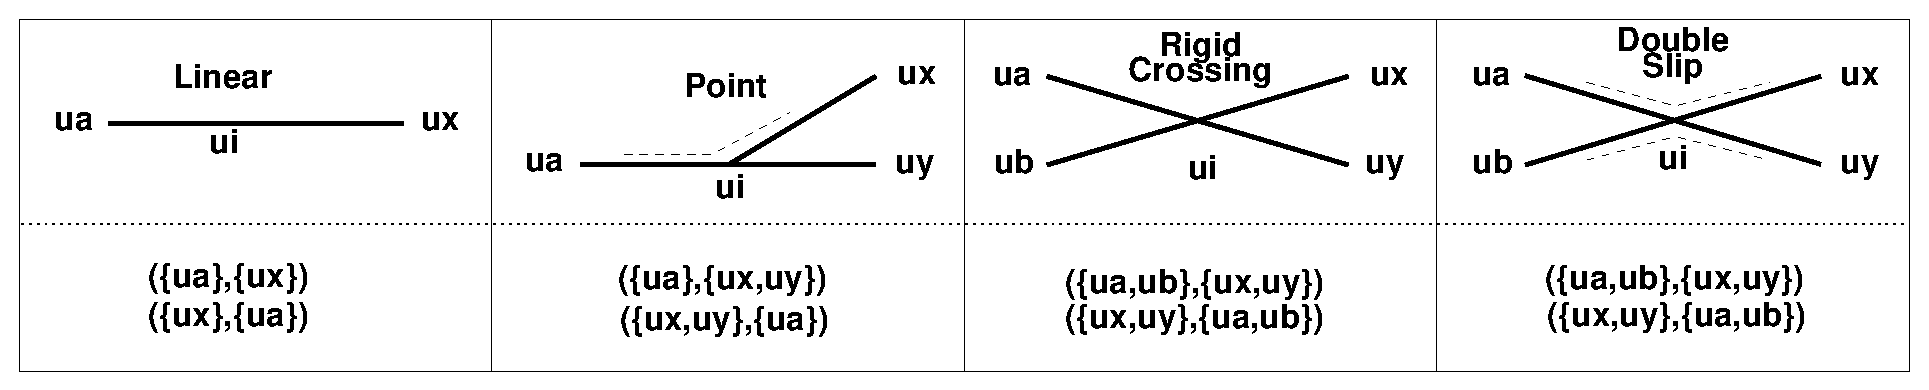
\epsfig{file=rail-mereo.eps,height=\pos{2.7}{5}cm}
\caption{Four Symmetric Rail Unit Mereologies\ \ \ \eod}\label{fig.rail-mereo}
\end{center}
\end{figure}

\label{lect3:labelmereo}

\pos{}{\mnewfoil
\label{lect3:label1a}
\ \vfill
\centerline{\lilacolor{Day \#{4}: Attributes and Summary}}
\vfill
}

\nbbbbb{Attributes}\label{chap4.Attributes}

\ysf{\dbeat{\pvienna{5.4}{119--139}}}

\noindent
\begynd
\pind To recall: there are three sets of
      \textbf{\pdindextermii{internal}{qualities}}:
\begynd
\pind \textsf{unique identifiers}, 
\pind \textsf{mereologies} and
\pind \textsf{attributes}. 
\afslut
\pind \textsf{Unique identifiers} and  \textsf{mereologies} \nyl
       are rather definite kinds of internal endurant qualities;
\pind \textsf{attributes} form more ``free-wheeling'' sets of
      \pdindextermii{internal}{qualities}.
\pind Whereas, for this \monograph, we suggest to not endow \nyl
fluids with unique identification and mereologies\ysfchg{. }

      \ysfchg{A}ll endurants, i.e., including fluids, are endowed with attributes. 
\afslut

\nbbbb{Inseparability of Attributes from Parts and Fluids}\label{technical issues}

\begynd
\pind Parts {and fluids} are 
\begynd
\pind typically recognised because of their spatial form
\pind and are otherwise characterised by their intangible, \nyl
      but measurable attributes. \pos{That is, whereas
      endurants, whether solid (as are parts) 
      or  fluids, are physical, tangible, in the sense of being
      spatial [or 
      being abstractions, i.e., concepts, of spatial endurants],
      attributes are intangible: cannot normally be
      touched\footnote{\LLLL One can see the red colour of a wall, but one
        touches the wall.}, or seen\footnote{One cannot see electric
        current, and one may touch an electric wire, but only if it
        conducts high voltage can one know that it is indeed an
        electric wire.}, but can
      be objectively measured\footnote{\LLLL That is, we restrict our domain
      analysis with respect to attributes to such quantities which are
      observable, say by mechanical, electrical or chemical
      instruments. Once objective measurements can be made of human
      feelings, beauty, and other, we may wish to include these
      ``attributes'' in our domain descriptions.}. Thus, in our quest
      for describing  
      domains where humans play an active r{\^o}le, we rule out
      subjective ``attributes'': feelings, sentiments, moods. Thus we
      shall abstain, in our domain science also from matters of
      aesthetics.}{} 
\afslut
    
 \pind We equate all endurants --- which have \nyl \LLLL \sfsl{the same type of unique
       identifiers, \nyl  the same type  of mereologies,  \nyl and the same types
       of attributes} \nyl \HHHH --- with one sort.
\pind Thus removing an internal quality from an endurant \nyl makes no sense:
\begynd \LLLL
\pind the endurant of that type 
\pind either becomes an endurant of another type
\pind or ceases to exist (i.e., becomes a non-entity)\,!
\afslut \HHHH
\mnewfoil

\pind We can roughly distinguish between two kinds of attributes:
\begynd
\pind those which can be motivated \nyl by \sort{physical}
      (incl\ysfchg{uding } chemical) \sort{concerns}, and
\pind those, \LLLL
\begynd
\pind which, although they embody some form of `physics measures',
\pind appear to reflect on \sort{event histories}: \LLLL
\begynd
\pind \sfsl{``if `something', $\phi$, has `happened' to an endurant, $e_a$,}
\pind \sfsl{then some `commensurate thing', $\psi$, has `happened' to
            another (one or more) endurants, $e_b$.''}
\afslut
\pind where the \sfsl{`something'} and \sfsl{`commensurate thing'}
\pind usually involve some `interaction' between the two (or more) endurants.
\afslut \HHHH
\pind It can take some reflection and analysis to properly identify \LLLL
\begynd
\pind endurants $e_a$ and $e_b$ and 
\pind commensurate events $\phi$ and $\psi$.
\afslut\HHHH
\pos{ 
\pind Example\,\ref{Intentional Pull -- Road Transport} shall illustrate the, as we shall call it,
      \bbcolor{intentional pull} of event histories.}{}
\afslut
\afslut

\nbbbb{Attribute Modelling Tools}\label{kap4.Attribute Modeling Tools}

\bbb{Attribute Quality and Attribute Value} \label{AQaAV} 
\begynd
\pind We distinguish between
\begynd
\pind an \bbcolor{attribute} (as a logical proposition, of a name, i.e.) \bbcolor{type}, and
\pind an \bbcolor{attribute value}, as a value in some value space.
\afslut
\afslut

\nbbb{Concrete Attribute Types}
\begynd
\pind By a \sfsl{concrete type}\pos{\index{dind}{concrete attribute
      type}\index{dind}{concrete!attribute!type}\index{dind}{type!concrete}\index{dind}{concrete!type}}{}
    \ysfchg{we } shall understand a sort (i.e., a type) which is defined in terms of
    some type expression: \textsf{T = $\mathcal{T}(...)$}.
\pind This is \ysf{indicated below by} \textsf{[=...]}.
\dbeat{We refer to
        Appendix Sect.\,\vref{tseb.rsl.Type Expressions} for more on \texttt{RSL} types.}
\afslut


\nbbb{Attribute Description}\label{pama:taf}\pos{\normalsize}{\HHHH}

\begynd
\pind Let us recall that attributes cover qualities \nyl other than
      unique identifiers and mereology.
\pind Let us then consider that parts and fluids \nyl \ysfchg{} have one or more attributes.
\begynd
\pind These attributes are qualities
\pind which help characterise ``what it means'' \nyl to be a part or a fluid.
\afslut 
\pind Note that we expect every part and fluid to have at least one attribute.
\pind The question is now, in general, \nyl how many and, particularly, which.
\afslut

\ysf{%%%
\begynd%%%
\pind The \bbcolor{\texttt{describe\_attributes}} description prompt
      is now defined.
\afslut%%%
}%%%

\mnewfoil\HHHH

\ddprompt{describe\_attributes}{observe-attributes}{\label{observeattributes}%%
\begynd\HHHH
\pind The domain analyser experiments, thinks and reflects \nyl about endurant,
      \textsf{e}, attributes. 
\pind That process is initiated by the \ddp:
\begin{itemize}
\item \texttt{describe\_attributes(e)}.\dodepr%
      \dpindex{describe\_attributes}%
\end{itemize}
\pind The result of that \ddp\ is \nyl that the domain analyser cum
      describer writes down \nyl the \ddtu{Attribute (Sorts or) Types and
        Observers}
\afslut
\mnewfoil\pos{}{\LLLL\HHHH}\bdbrule
\pos{}{{\bgcolor{\bgcolor{\cdlti}\ \texttt{describe\_attributes}} \sort{Observer}}}
      \delati{describe\_attributes}%
      \ddlt{PartAttributes}{dlti}
%\RSLatex
%let {&$\eta$A$_1$, ..., $\eta$A$_m$&} = determine_attribute_type_names(e) in     
%&\bq\kw{Narration:}&
%      [t]    ... &narrative text on attribute sorts& ...
%          &\,\,\,\,some \textsf{Ai}s may be concretely defined: [Ai=...]&
%      [o] &\,&  ... narrative text on attribute sort observers ...
%      [p] &\,&  ... narrative text on attribute sort proof obligations ...
%& \kw{Formalisation:}&
%      type
%      [t]   A&$_1$[=...]& , ...,  A&$_m$[=...]&
%      value
%      [o]   &{\attrmo}&A&$_1$&: E->A&$_1$&, ..., &{\attrmo}&A&$_m$&: E->A&$_m$&&\delaoi{\protect{\attrmo}}\label{attrAi}&
%      &\kw{proof obligation}& [Disjointness &of& Attribute Types]
%      [p]    &$\mathcal{PO}$:& &\poindex{podoats2}{\protect{$\mathcal{PO}:$} Disjointness of Attribute Types}&let P & be any part sort& in &[the domain description]&&\label{attribute-po}&
%      [p]            let a:(A&$_1$&|A&$_2$&|...|A&$_m$&) in &{\ismo}&A&$_i$&(a) ~= &{\ismo}&A&$_j$&(a) [i~=i, i,j:[1..m]] end end &\eq&
% end
%\endRSLatex 
\bp
\kw{let} {\LBRACE}$\eta$A$_1$, ..., $\eta$A$_m${\RBRACE} {\EQ} determine\_attribute\_type\_names(e) \kw{in}\ \ \ \ \ \\
\bq\kw{Narration:}\\
\>\>\>{\LBRACKET}t{\RBRACKET}\ \ \ \ {\DOTDOTDOT} narrative text on attribute sorts {\DOTDOTDOT}\\
\>\>\>\>\>\,\,\,\,some \textsf{Ai}s may be concretely defined: [Ai=...]\\
\>\>\>{\LBRACKET}o{\RBRACKET} \,\ \ {\DOTDOTDOT} narrative text on attribute sort observers {\DOTDOTDOT}\\
\>\>\>{\LBRACKET}p{\RBRACKET} \,\ \ {\DOTDOTDOT} narrative text on attribute sort proof obligations {\DOTDOTDOT}\\
 \kw{Formalisation:}\\
\>\>\>\kw{type}\\
\>\>\>{\LBRACKET}t{\RBRACKET}\ \ \ A$_1$[=...] , {\DOTDOTDOT},\ \ A$_m$[=...]\\
\>\>\>\kw{value}\\
\>\>\>{\LBRACKET}o{\RBRACKET}\ \ \ {\attrmo}A$_1$: E{\RIGHTARROW}A$_1$, {\DOTDOTDOT}, {\attrmo}A$_m$: E{\RIGHTARROW}A$_m$\delaoi{\protect{\attrmo}}\label{attrAi}\\
\>\>\>\kw{proof obligation} {\LBRACKET}Disjointness of Attribute Types{\RBRACKET}\\
\>\>\>{\LBRACKET}p{\RBRACKET}\ \ \ \ $\mathcal{PO}$: \poindex{podoats2}{\protect{$\mathcal{PO}:$} Disjointness of Attribute Types}\kw{let} P  be any part sort \kw{in} [the domain description]\label{attribute-po}\\
\>\>\>{\LBRACKET}p{\RBRACKET}\ \ \ \ \ \ \ \ \ \ \ \ \kw{let} a:(A$_1${\BAR}A$_2${\BAR}{\DOTDOTDOT}{\BAR}A$_m$) \kw{in} {\ismo}A$_i$(a) {\NOTEQ} {\ismo}A$_j$(a) {\LBRACKET}i{\NOTEQ}i, i,j:{\LBRACKET}1{\DOTDOT}m{\RBRACKET}{\RBRACKET} \kw{end} \kw{end} \eq\\
 \kw{end}
\ep
\edbrule
}

\noindent%
\pos{\psno}{\mnewfoil}%
\begynd%
\pind Let \textsf{A$_1$, ..., A$_n$} be the set of all
      conceivable attributes of endurant\ysfchg{ } $e$:$E$. 
\begynd
\pind (Usually $n$ is a
      rather large natural number, say in the order of a hundred
      conceivable such.) 
\pind In any one domain model the domain analyser
      cum describer selects a modest subset, \textsf{A$_1$,
        ..., A$_m$}, i.e., ${m}<{n}$. 
\pind Across many domain models \nyl for
      \textsl{``more-or-less the same''} domain $m$ varies \nyl and the
      attributes, \textsf{A$_1$,  ..., A$_m$}, \nyl selected for one
      model may differ \nyl from those, \textsf{A$'_1$, ..., A$'_{m'}$},
      chosen for another model.
\afslut
\mnewfoil
       
\pind The \kw{type} definitions: 
      \textsf{A$_1$, ..., A$_m$},
      inform us that the domain analyser has decided to focus
      on the distinctly named \textsf{A$_1$, ..., A$_m$}
      attributes.\pos{\footnote{\LLLL The attribute type names
      are chosen by the domain analyser to
      reflect on domain phenomena.}}{}
\pind The \kw{value} clauses 
\begynd
\pind \textsf{\small\HHHH{\attrmo}A$_1$:P{\RIGHTARROW}A$_1$, 
\pind  {\DOTDOTDOT},
\pind       {\attrmo}A$_n$:P{\RIGHTARROW}A$_n$} 
\afslut \normalsize\HHHH
      are then ``automatically'' given:
\begynd
\pind if an endurant, \textsf{e:E}, has an attribute \textsf{A$_i$}
\pind then there is postulated, ``by definition'' [eureka] 
      \pos{}{\\} an attribute
      observer function
      \textsf{\small\HHHH{\attrmo}A$_i$:E{\RIGHTARROW}A$_i$}
      et cetera\dbsquare\ 
\afslut
\afslut\pos{\normalsize}{\HHHH}
\mnewfoil

\begynd
\pind We cannot automatically, that is, syntactically, \nyl
      guarantee that our domain descriptions secure that
\begynd
\pind the various attribute types
\pind for a\ysfchg{n } endurant sort 
\pind denote disjoint sets of values. 
\afslut
      Therefore we must prove it. 
\afslut

\nbbb{Attribute Categories}\label{Attribute Categories}

\begynd
\pind Michael A.\ Jackson \cite{lexicon} has suggested a hierarchy of
      attribute categories:
\begynd
\pind from static
\pind to dynamic values -- and within the dynamic value category:
\begynd
\pind inert values,
\pind reactive values, 
\pind active values -- and within the dynamic active value category:
\begynd
\pind autonomous values,
\pind biddable values and
\pind programmable values.
\afslut
\afslut  
\afslut%
\pind We now review these attribute value types. \nyl
      The review is based on \pos{\cite[M.A.Jackson]{lexicon}}{\cite[M.A.Jackson]{lexicon}}.
\afslut%
\mnewfoil%

\begynd
\pind \sfsl{{Endurant attributes}} are 
\begynd
\pind either constant, i.e.,  \bmcolor{{static}}, 
\pind or varying, i.e., \bmcolor{{dynamic}}  
\afslut attributes\ysfchg{. }
\afslut
%%%
%%% STATIC
%%%

\attribute{static}{\begynd
\pind By a \label{staticattribute}
      {\pdindexii{static}{attribute}}, \textsf{{a:A}},
      \bbcolor{\protect{\texttt{is\_static\_attribute}}}({\textsf{a}}),%
      \sac\atindex{\protect{is\_static\_attribute}} \nyl
      we shall understand an attribute whose values
\begynd
\pind are constants,
\pind i.e., cannot change\dbsquare
\afslut
\afslut}
\mnewfoil
\monoexample{Static Attributes}{%
\begynd
\pind Let us exemplify road net attributes \nyl in this and the next examples.
\pind And let us assume the following attributes:
\begynd
\pind year of first link construction and
\pind link length at that time.
\afslut
\pind We may consider both to be static attributes:
\begynd
\pind The year first established, \nyl seems an obvious static attribute and
\pind the length is fixed at the time the road was first built.
\afslut
\afslut
}

%%%
%%% DYNAMIC
%%%
\mnewfoil\label{Dynamic Attribute Categories}
\attribute{dynamic}{\begynd\label{dynamicattribute}
  \pind By a {\pdindexii{dynamic}{attribute}}, \textsf{{a:A}},
      \bbcolor{\texttt{is\_dynamic\_attribute}}({\textsf{a}}),% 
      \sac\atindex{is\_dynamic\_attribute}\pos{}{\\}
      we shall understand an attribute whose values
\begynd
\pind are variable, 
\pind i.e., can change.
\afslut
{{Dynamic attributes}} are either \sfsl{inert, reactive}
or \sfsl{active} attributes\dbsquare
\afslut}
%%%%
%%%% INERT
%%%%
\mnewfoil
\attribute{inert}{
\begynd\label{inertattribute}
\pind By an \lilacolor{\pdindexii{inert}{attribute}}, \textsf{a:A},
      \bbcolor{\texttt{is\_\-in\-ert\_\-at\-tri\-bute}}(\textsf{a}),% 
      \sac\atindex{is\_inert\_attribute}\pos{}{\\}
      we shall understand a dynamic attribute whose values
\begynd
\pind only change as the result of external stimuli where 
\pind these stimuli prescribe new values\dbsquare
\afslut 
\afslut}
\mnewfoil
\monoexample{Inert Attribute}{%
\begynd
\pind And let us now further assume the following link attribute:
\begynd
\pind link name.
\afslut
\pind We may consider it to be an inert attribute:
\begynd
\pind the name is not ``assigned'' to the link by the link itself,
\pind but probably by some road net authority 
\pind which we are not modelling.
\afslut
\afslut
  }%%%
%%% REACTIVE
%%%
\mnewfoil
\attribute{reactive}{\label{reactiveattribute}
\begynd
\pind By a \bbcolor{\pdindexii{reactive}{attribute}}, \textsf{a:A}, 
      \bbcolor{\texttt{is\_reactive\_attribute}}(\textsf{a}),% 
      \sac\atindex{is\_reactive\_attribute}\pos{}{\\}
      we shall understand a dynamic attribute  whose values, 
\begynd
\pind if they vary, change  in response to external stimuli,
\pind where these stimuli  
\begynd
\pind either come from outside the domain of interest
\pind or from other endurants\dbsquare
\afslut
\afslut
\afslut
}
\mnewfoil

\monoexample{Reactive Attributes}{%
\begynd
\pind Let us further assume the following two link attributes:
\begynd
\pind ``wear and tear'', respectively
\pind ``icy and slippery''.
\afslut
\pind We will consider those attributes to be reactive in that
\begynd
\pind automobiles (another part) traveling the link, an external ``force'', \nyl
      typically causes the ``wear and tear'', respectively
\pind the weather (outside our domain) \nyl causes the  ``icy and slippery'' property.
\afslut
\afslut
}
%%%
%%% ACTIVE
%%%
\mnewfoil
\attribute{active}{\label{activeattribute}
\begynd
\pind By an \bbcolor{\pdindexii{active}{attribute}}, \textsf{a:A},
      \bbcolor{\texttt{is\_active\_attribute}}(\textsf{a}),% 
      \sac\atindex{is\_active\_attribute}\pos{}{\\}
      we shall understand a  dynamic attribute whose values 
\begynd
\pind change (also) \ysfchg{by } its own volition.
\afslut
{{Active attributes}} are 
\begynd
\pind either \sfsl{autonomous}, 
\pind or \sfsl{biddable} 
\pind or \sfsl{programmable}
\afslut attributes\dbsquare
\afslut}
%%%
%%% AUTONOMOUS
%%%
\mnewfoil
\attribute{autonomous}{\label{autonomousattribute}
\begynd
\pind By an \dindexii{autonomous}{attribute}, \textsf{a:A},
      \bbcolor{\texttt{is\_autonomous\_attribute}}(\textsf{a}),% 
      \sac\atindex{is\_autonomous\_attribute}\pos{}{\\}
      we shall understand a dynamic active attribute %\fromitemize 
\begynd
\pind whose values change only ``on their own volition''. 
\pind The values
      of an autonomous attributes \nyl are a ``law onto 
      themselves and their surroundings''\dbsquare
\afslut
\afslut}
\mnewfoil
\monoexample{Autonomous Attributes}{\LLLL\HHHH%
\begynd
\pind We enlarge \ysfchg{the } scope of our examples of attribute categories to now
      also include automobiles (on the road net).
\pind In this example we assume that an automobile is driven by a
      human [behaviour].
\pind These are some automobile attributes:
\begynd
\pind velocity,
\pind acceleration, and
\pind moving straight, or turning left, or turning right.
\afslut
\pind We shall consider these three attributes to be autonomous.
\begynd
\pind It is the driver, not the automobile, who decides
\pind whether the automobile should drive at constant velocity,
including 0, or accelerate or decelerate, including stopping.
\pind And it is the driver who decides when to turn left or right, or
not turn at all.
\afslut
\afslut
}
\mnewfoil
%%%
%%% BIDDABLE
%%%
\attribute{biddable}{\label{biddableattribute}
\begynd
\pind By a \lilacolor{\pdindexii{biddable}{attribute}}, \textsf{a:A},
      \bbcolor{\texttt{is\_\-bid\-dable\_\-at\-tri\-bute}}(\textsf{{\small\HHHH
          a}})\label{biddable}%  
      \sac\atindex{is\_biddable\_attribute} \nyl we shall understand a 
      {dynamic} {active} attribute whose values \faocb
\begynd
\pind \sfsl{are prescribed
\pind but may fail to be observed as \ysf{retaining that value}}\dbsquare
\afslut
\afslut}
\mnewfoil


\monoexample{Biddable Attributes}{In the context of automobiles these
  are some biddable attributes:
\begynd
\pind turning the wheel, to drive right at a hub \nyl -- with the
      automobile failing to turn right;
\pind pressing the accelerator, to obtain a higher speed \nyl --
      with the automobile failing to really gaining speed;
\pind pressing the brake, to stop \nyl --
      with the automobile failing to halt\dbsquare
\afslut}

%%%
%%% PROGRAMMABLE
%%%
\mnewfoil
\attribute{programmable}{\label{programmableattribute}
\begynd
\pind By a \lilacolor{\pdindexii{programmable}{attribute}},
      \textsf{a:A}, 
      \bbcolor{\texttt{is\_\-pro\-gram\-mable\_\-at\-tri\-bute}}(\textsf{a}),% 
      \sac\atindex{is\_programmable\_attribute}
      we shall understand a
      {dynamic} {active} attribute whose values
\begynd
\pind can be prescribed\dbsquare
\afslut
\afslut}
\mnewfoil
\monoexample{Programmable Attribute}{%
\begynd
\pind We continue with the automobile on the road net examples.
\pind In this example we assume that an automobile includes, as one
      inseparable entity, ``the driver''.
\pind These are some automobile attributes:
\begynd
\pind position on a link,
\pind velocity, acceleration (incl.\ deceleration), and
\pind direction: straight, turning left, turning right.
\afslut
\pind We shall now consider these three attributes to be programmable.
\afslut
}
\noindent
\pos{\psno}{\mnewfoil}
\begynd
\pind Figure\,\ref{attributes.fig} captures an attribute value ontology.
\afslut

\pos{\hDBfigure{attributes}{4cm}{Attribute Value Ontology}{attributes.fig}}%
    {\hDBfigure{attributes}{10cm}{Attribute Value Ontology}{attributes.fig}}


\noindent%
\pos{\psno}{\mnewfoil}%
\begynd%
\pind Figure\,\ref{attributes.fig} hints at three categories of
      dynamic attributes:
\begynd
\pind \bbcolor{monitorable only},
\pind \bbcolor{biddable} and
\pind \bbcolor{programmable}
\afslut
attributes.
\afslut
\mnewfoil

\attribute{monitorable only}{\label{monitorableattribute}
\begynd
\pind By a \lilacolor{\pdindexii{monitorable only}{attribute}},
      \textsf{a:A},  \nyl
      \bbcolor{\texttt{is\_monitorable\_only\_at\-tri\-bute}}(\textsf{a}),% 
      \sac\atindex{is\_monitorable\_only\_attribute} \nyl
      we shall understand a
      {dynamic} {active} attribute which is either
\begynd
\pind \sfsl{inert} or
\pind \sfsl{reactive} or
\pind \sfsl{autonomous}.
\afslut
\afslut} 
\noindent
That is:

%\RSLatex
%   value  
%      is_monitorable_only: E -> Bool
%      is_monitorable_only(e) is is_inert(e) \/ is_reactive(e) \/ is_autnomous(e)
%\endRSLatex 
\bp
\>\ \kw{value}\ \ \\
\>\>\>is\_monitorable\_only: E {\RIGHTARROW} \kw{Bool}\\
\>\>\>is\_monitorable\_only(e) {\IS} is\_inert(e) {\VEE} is\_reactive(e) {\VEE} is\_autonomous(e)
\ep


\mnewfoil

\monoexample{Road Net Attributes}
\noindent\LLLL\HHHH
\begynd
\pind We treat some attributes of the hubs of a road net.
\afslut
\begin{enumerate}\setei
\item \label{h-attr-000} There is a hub state.
\begynd
\pind  It is a set of pairs, \textsf{(l$_f$,l$_t$)}, of link identifiers,
\begynd
\pind  where these link identifiers are in the mereology of the hub. 
\afslut
\pind The meaning of the hub  state
\begynd
\pind in which, e.g., \textsf{(l$_f$,l$_t$)} is an element, 
\pind is that the hub is open,  \bgcolor{``green''}, 
\pind for traffic $f$rom link \textsf{l$_f$} $t$o link \textsf{l$_t$}.  
\pind If a hub state is empty
\pind then the hub is closed, i.e., \brcolor{``red''} 
\pind for traffic from any
                         connected links to any other connected links.
\afslut
\afslut
\pos{\psno}{\mnewfoil}
\item \label{h-attr-010} There is a hub state space.
\begynd
\pind It is a set of hub states. 
\pind The current hub state must be in its state space.
\pind The meaning of the hub state space is 
\begynd
\pind that its states are all those the hub can attain.
\afslut
\afslut
\item \label{hub-traffic} Since we can think rationally about it,
\begynd
\pind it can be described, hence we can model, as an
                          attribute of hubs, a history of its traffic:
\begynd
\pind the recording, per unique automobile identifier, 
\pind of the time ordered presence in the hub of these vehicles.   
\afslut
\pind Hub history is an \sfsl{event history}.
\afslut
\savei\end{enumerate}
\pos{\psno}{\mnewfoil}
\pos{\footsize}{\LLLL\HHHH\sf}
%\pos{\begin{multicols}{2}}{}
%\RSLatex
%type
%&\ref{h-attr-000}&  H`Sigma = (L_UI><L_UI)-set
%&\ref{h-attr-010}&  H`Omega = H`Sigma-set
%&\ref{hub-traffic}&  H_Traffic = A_UI -m-> (&$\mathbb{TIME}$& >< VPos)-list
%axiom
%&\ref{h-attr-000}&  all h:H :- obs_H`Sigma(h) isin obs_H`Omega(h)
%&\ref{hub-traffic}&  all ht:H_Traffic,ui:A_UI :-  ui isin dom ht => time_ordered(ht(ui))
%value 
%&\ref{h-attr-000}&  attr_H`Sigma: H -> H`Sigma
%&\ref{h-attr-010}&  attr_H`Omega: H -> H`Omega 
%&\ref{hub-traffic}&  attr_H_Traffic: H -> H_Traffic
%&\ref{hub-traffic}&   time_ordered: (&$\mathbb{TIME}$& >< VPos)-list -> Bool
%&\ref{hub-traffic}&   time_ordered(tvpl) is ...
%\endRSLatex  
\bp
\kw{type}\\
\ref{h-attr-000}\ \ H$\Sigma$ {\EQ} (L\_UI{\TIMES}L\_UI)\kw{-set}\\
\ref{h-attr-010}\ \ H$\Omega$ {\EQ} H$\Sigma$\kw{-set}\\
\ref{hub-traffic}\ \ H\_Traffic {\EQ} A\_UI {\MARROW} ($\mathbb{TIME}$ {\TIMES} VPos)$^{\ast}$\\
\kw{axiom}\\
\ref{h-attr-000}\ \ {\ALL} h:H {\RDOT} obs\_H$\Sigma$(h) {\ISIN} obs\_H$\Omega$(h)\\
\ref{hub-traffic}\ \ {\ALL} ht:H\_Traffic,ui:A\_UI {\RDOT}\ \ ui {\ISIN} \kw{dom} ht {\DBLRIGHTARROW} time\_ordered(ht(ui))\\
\kw{value} \\
\ref{h-attr-000}\ \ attr\_H$\Sigma$: H {\RIGHTARROW} H$\Sigma$\\
\ref{h-attr-010}\ \ attr\_H$\Omega$: H {\RIGHTARROW} H$\Omega$ \\
\ref{hub-traffic}\ \ attr\_H\_Traffic: H {\RIGHTARROW} H\_Traffic\\
\ref{hub-traffic}\ \ \ time\_ordered: ($\mathbb{TIME}$ {\TIMES} VPos)$^{\ast}$ {\RIGHTARROW} \kw{Bool}\\
\ref{hub-traffic}\ \ \ time\_ordered(tvpl) {\IS} {\DOTDOTDOT}
\ep
%\pos{\end{multicols}}{}
\pos{\normalsize}{\HHHH}\rm
\noindent
\begynd
\pind In Item\,\ref{hub-traffic} we model the time-ordered sequence
      of traffic as a discrete sampling, i.e., {\MARROW}, rather than as a
      continuous function, {\RIGHTARROW} \eod
\afslut

\pos{\psno}{\mnewfoil}
\monoexample{Invariance of Road Net Traffic States}{
\begynd
\pind We continue Example\,\vref{Road Net Attributes}.
\afslut
\begin{enumerate}\setei
\item \label{h-attr-030} The link identifiers of hub states must be in
                         the set, $l_{ui}s$, of the road net's link
                         identifiers.
\savei\end{enumerate}
%\RSLatex
%axiom
%&\ref{h-attr-030}&  all h:H :- h isin &$hs$& => 
%&\ref{h-attr-030}&      let h`sigma = attr_H`Sigma(h) in 
%&\ref{h-attr-030}&      all (l&$_{ui}i$&,li&$_{ui}i'$&):(L_UI><L_UI) :- (l&$_{ui}i$&,l&$_{ui}i'$&) isin h`sigma => {l&$_{ui_i}$&,l&$_{ui_i}'$&} <<= l&$_{ui}s$& end &\eod&
%\endRSLatex
\bp
\kw{axiom}\\
\ref{h-attr-030}\ \ {\ALL} h:H {\RDOT} h {\ISIN} $hs$ {\DBLRIGHTARROW} \\
\ref{h-attr-030}\ \ \ \ \ \ \kw{let} h$\sigma$ {\EQ} attr\_H$\Sigma$(h) \kw{in} \\
\ref{h-attr-030}\ \ \ \ \ \ {\ALL} (l$_{ui}i$,li$_{ui}i'$):(L\_UI{\TIMES}L\_UI) {\RDOT} (l$_{ui}i$,l$_{ui}i'$) {\ISIN} h$\sigma$ {\DBLRIGHTARROW} {\LBRACE}l$_{ui_i}$,l$_{ui_i}'${\RBRACE} {\SUBSETEQ} l$_{ui}s$ \kw{end} \eod
\ep
}%
\noindent%
\pos{\psno}{\mnewfoil}%
\begynd%
\pind You may skip Example\,\vref{Road Transport -- Further Attributes} in a first reading.
\afslut

\monoexample{Road Transport -- Further Attributes}{

  \bmcolor{Links:}

  We show just a few attributes.

\pos{\bmcii}{}
\begin{enumerate}\setei
\item \label{l-attr-000} There is a link state. It is a set of pairs,
                         \textsf{(h$_f$,h$_t$)}, of distinct hub identifiers,
                         where these hub identifiers are in the
                         mereology of the link. The meaning of a link
                         state in which \textsf{(h$_f$,h$_t$)} is an
                         element is that the link is open, 
                         \bgcolor{``green''}, for traffic $f$rom hub
                         \textsf{h$_f$} $t$o hub \textsf{h$_t$}.  Link
                         states can have either 0, 1 or 2 elements.
\item \label{l-attr-010} There is a link state space. It is a set of
                         link states.  The meaning of the link state
                         space is that its states are all those \ysf{}
                         which the link can attain. The current link state must be
                         in its state space. If a link state space is
                         empty then the link is \ysf{}
                         closed. If it has one element then it is a
                         one-way link. If a one-way link, $l$, is imminent
                         on a hub whose mereology designates that
                         link, then the link is a ``trap'', i.e., a
                         ``blind cul-de-sac''. 
\mnewfoil
\item \label{link-traffic} Since we can think rationally about it, it
                          can be described, hence it  can model, as an
                          attribute of links\ysf{,} a  history of its traffic:
                          the recording, per unique \ysf{}
                          automobile identifier, of the time ordered
                          positions along the link (from one hub to
                          the next) of these vehicles.  
\item \label{l-attr-030} The hub identifiers of link states must be in
                         the set, $h_{ui}s$, of the road net's hub
                         identifiers. 
\savei\end{enumerate}
\mnewfoil
\footsize\LLLL\HHHH
%\RSLatex
%type
%&\ref{l-attr-000}&  L`Sigma = (H_UI><H_UI)-set
%&\ref{l-attr-010}&  L`Omega = L`Sigma-set  
%&\ref{link-traffic}&  L_Traffic       
%&\ref{link-traffic}&  L_Traffic = A_UI -m-> (&$\mathbb{T}$&><(H_UI><Frac><H_UI))-list      
%&\ref{link-traffic}&  Frac = Real, axiom frac:Fract :- 0<frac<1
%value 
%&\ref{l-attr-000}&  attr_L`Sigma: L -> L`Sigma
%&\ref{l-attr-010}&  attr_L`Omega: L -> L`Omega
%&\ref{link-traffic}&  attr_L_Traffic: : -> L_Traffic
%axiom
%&\ref{l-attr-000}&  all l`sigma:L`Sigma:-card l`sigma<=2
%&\ref{l-attr-000}&  all l:L :- obs_L`Sigma(l) isin obs_L`Omega(l)
%&\ref{link-traffic}&  all lt:L_Traffic,ui:A_UI:-ui isin dom ht => time_ordered(ht(ui))
%&\ref{l-attr-030}&  all l:L:-l isin &$ls$& =>
%&\ref{l-attr-030}&     let l`sigma =attr_L`Sigma(l) in all (h&$_{ui}i$&,h&$_{ui}i'$&):(H_UI><H_UI):-&(h$_{ui}i$&,h&$_{ui}i'$)&isin l`sigma=>{h&$_{ui_i}$&,h&$_{ui_i}'$&}<<=h&$_{ui}s$& end
%\endRSLatex 
\bp
\kw{type}\\
\ref{l-attr-000}\ \ L$\Sigma$ {\EQ} (H\_UI{\TIMES}H\_UI)\kw{-set}\\
\ref{l-attr-010}\ \ L$\Omega$ {\EQ} L$\Sigma$\kw{-set}\ \ \\
\ref{link-traffic}\ \ L\_Traffic\ \ \ \ \ \ \ \\
\ref{link-traffic}\ \ L\_Traffic {\EQ} A\_UI {\MARROW} ($\mathbb{T}${\TIMES}(H\_UI{\TIMES}Frac{\TIMES}H\_UI))$^{\ast}$\ \ \ \ \ \ \\
\ref{link-traffic}\ \ Frac {\EQ} \kw{Real}, \kw{axiom} frac:Fract {\RDOT} 0{\LT}frac{\LT}1\\
\kw{value} \\
\ref{l-attr-000}\ \ attr\_L$\Sigma$: L {\RIGHTARROW} L$\Sigma$\\
\ref{l-attr-010}\ \ attr\_L$\Omega$: L {\RIGHTARROW} L$\Omega$\\
\ref{link-traffic}\ \ attr\_L\_Traffic: : {\RIGHTARROW} L\_Traffic\\
\kw{axiom}\\
\ref{l-attr-000}\ \ {\ALL} l$\sigma$:L$\Sigma${\RDOT}\kw{card} l$\sigma${\LEQ}2\\
\ref{l-attr-000}\ \ {\ALL} l:L {\RDOT} obs\_L$\Sigma$(l) {\ISIN} obs\_L$\Omega$(l)\\
\ref{link-traffic}\ \ {\ALL} lt:L\_Traffic,ui:A\_UI{\RDOT}ui {\ISIN} \kw{dom} ht {\DBLRIGHTARROW} time\_ordered(ht(ui))\\
\ref{l-attr-030}\ \ {\ALL} l:L{\RDOT}l {\ISIN} $ls$ {\DBLRIGHTARROW}\\
\ref{l-attr-030}\ \ \ \ \ \kw{let} l$\sigma$ {\EQ}attr\_L$\Sigma$(l) \kw{in} {\ALL} (h$_{ui}i$,h$_{ui}i'$):(H\_UI{\TIMES}H\_UI){\RDOT}(h$_{ui}i$,h$_{ui}i'$){\ISIN} l$\sigma${\DBLRIGHTARROW}{\LBRACE}h$_{ui_i}$,h$_{ui_i}'${\RBRACE}{\SUBSETEQ}h$_{ui}s$ \kw{end}
\ep
\pos{\emcii}{}\smallish\LLLL

\vspace*{1mm}
\mnewfoil

\noindent
\bmcolor{Automobiles:}
\begynd
\pind We illustrate but a few attributes:
\afslut
\begin{enumerate}\setei
\item \label{a-attr-000} Automobiles have static number plate
                         registration numbers.
\item \label{a-attr-005} Automobiles have dynamic positions on the road net:
\begin{enumerate}
\item\label{a-attr-005a} either \sfsl{at a hub} identified by some \textsf{h\_ui}, 
\item\label{a-attr-005b} or \sfsl{on a link}, some \sfsl{fraction, frac:Fract} down an
                         \sfsl{identified link, l\_ui}, from one of
                         its \sfsl{identified connecting hub}s, \textsf{fh\_ui}, in the 
                         direction of the other \sfsl{identified hub},
                         \textsf{th\_ui}. 
\item\label{a-attr-005c} Fraction is a real properly between 0 and 1.
\end{enumerate}
\savei\end{enumerate}\footsize
\mnewfoil

%\RSLatex
%type
%&\ref{a-attr-000}&   RegNo
%&\ref{a-attr-005}&   APos == atHub | onLink
%&\ref{a-attr-005a}&  atHub :: h_ui:H_UI &\pos{\tidxi{A: atHub::H\_UI}{a-attr-005a}}{}&
%&\ref{a-attr-005b}&  onLink :: fh_ui:H_UI >< l_ui:L_UI >< frac:Fract >< th_ui:H_UI&\pos{\tidxi{A: onLink::H\_UI{\TIMES}L\_UI{\TIMES}Fract{\TIMES}H\_UI}{a-attr-005b}}{}&
%&\ref{a-attr-005c}&  Fract = Real
%axiom
%&\ref{a-attr-005c}&  frac:Fract :- 0<frac<1 &\pos{\tidxi{A: Frac{\EQ}\kw{Real}}{a-attr-005 0}}{}&
%value  
%&\ref{a-attr-000}&   attr_RegNo: A -> RegNo&\pos{\afidxi{A: attr\_RegNo}{a-attr-000}}{}& 
%&\ref{a-attr-005}&   attr_APos: A -> APos&\pos{\afidxi{A: attr\_APos}{a-attr-005}}{}& 
%\endRSLatex 
\bp
\kw{type}\\
\ref{a-attr-000}\ \ \ RegNo\\
\ref{a-attr-005}\ \ \ APos {\EQ}{\EQ} atHub {\BAR} onLink\\
\ref{a-attr-005a}\ \ atHub :: h\_ui:H\_UI \pos{\tidxi{A: atHub::H\_UI}{a-attr-005a}}{}\\
\ref{a-attr-005b}\ \ onLink :: fh\_ui:H\_UI {\TIMES} l\_ui:L\_UI {\TIMES} frac:Fract {\TIMES} th\_ui:H\_UI\pos{\tidxi{A: onLink::H\_UI{\TIMES}L\_UI{\TIMES}Fract{\TIMES}H\_UI}{a-attr-005b}}{}\\
\ref{a-attr-005c}\ \ Fract {\EQ} \kw{Real}\\
\kw{axiom}\\
\ref{a-attr-005c}\ \ frac:Fract {\RDOT} 0{\LT}frac{\LT}1 \pos{\tidxi{A: Frac{\EQ}\kw{Real}}{a-attr-005 0}}{}\\
\kw{value}\ \ \\
\ref{a-attr-000}\ \ \ attr\_RegNo: A {\RIGHTARROW} RegNo\pos{\afidxi{A: attr\_RegNo}{a-attr-000}}{} \\
\ref{a-attr-005}\ \ \ attr\_APos: A {\RIGHTARROW} APos\pos{\afidxi{A: attr\_APos}{a-attr-005}}{} 
\ep
\mnewfoil\smallish\HHHH
\noindent
\begynd
\pind Obvious attributes that are not illustrated are those of
\begynd
\pind velocity and acceleration, 
\pind forward or backward movement, 
\pind turning right, left or going straight, 
\pind etc.
\afslut
\afslut
\mnewfoil
\noindent
\begynd
\pind The \sfsl{acceleration, deceleration, even velocity,} or \sfsl{turning 
      right, turning left, moving straight}, or \sfsl{forward} or
      \sfsl{backward} are seen as \sfsl{command actions}. 
\begynd
\pind As such they denote actions by the automobile ---
\pind such as \textsf{pressing the accelerator}, or \textsf{lifting
      accelerator pressure} or 
      \sfsl{braking}, or \sfsl{turning the wheel} in one direction or
      another, etc.
\pind As actions they have a kind of counterpart in the
      \textsf{vel}ocity, the \textsf{acc}eleration, etc. attributes.
\afslut
\afslut
\pos{\emcii}{}
\mnewfoil\smallish\HHHH
\begynd
\pind In Items\,\psref{hub-traffic} and \psref{link-traffic}, 
      we illustrated an aspect of domain 
      analysis \& description that may seem, and at least some decades
      ago would have seemed, strange: namely that if we can think,
      hence speak, about it, then we can model it ``as a fact'' in the
      domain. The case in point is that we include among hub and link
      attributes their histories of the timed whereabouts of \ysf{ }
      automobiles\footnotemark\dbsquare
\afslut
}\footnotetext{In this day and age of road cameras and
        satellite surveillance these traffic recordings may not appear
        so strange: We now know, at least in principle, of
        technologies that can record approximations to the hub and
        link traffic attributes.} 
\pos{\psno}{\mnewfoil}

\nbbb{Calculating Attribute Category Type Names}\label{Calculating Attribute Category Types}

                                %\input{attributes}

\begynd
\pind One can calculate sets of all attribute type names, of static,
      \ysf{} monitorable and programmable attribute types of parts and
      fluids with the following \dap{s}:
\begin{itemize}
\item \bcolor{\texttt{determine\_attr\_\ysfchg{names}}},
\item \bcolor{\texttt{sta\_attr\_types}},
\item \bcolor{\texttt{mon\_attr\_types}}, and
\item \bcolor{\texttt{pro\_attr\_types}}.
\end{itemize}
\noindent
\begynd
\pind \texttt{determine\_att\ysfchg{r}\_type\_names} applies to parts and
      yields a set of all attribute names of that part.
\pind \texttt{sta\_attr\_types} applies to parts and
      yields a set of attribute names of \sfsl{static} attributes
      of that part.\footnote{\LLLL $\eta\mathbb{A}$ is the type of all
      attribute types.}
\pind \texttt{mon\_attr\_types} applies to parts and
      yields a set of attribute names of \sfsl{monitorable} attributes
      of that part.
\pind \texttt{pro\_attr\_types} applies to parts and
      yields a set of attribute names of \sfsl{programmable} attributes
      of that part.
\afslut
\afslut
\mnewfoil
\dafprompt{determine\_attr\_type\_names}{analyse-attribute-types}{\label{analysisattributes}%%
%\RSLatex
%    value
%        determine_attr_type_names: P -> `eta&A&-set
%        determine_attr_type_names(p) as {`eta&A1&,`eta&A&,...,`eta&Am& }
%\endRSLatex
\bp
\>\>\kw{value}\\
\>\>\>\>determine\_attr\_type\_names: P {\RIGHTARROW} $\eta$A\kw{-set}\\
\>\>\>\>determine\_attr\_type\_names(p) \kw{as} {\LBRACE}$\eta$A1,$\eta$A,{\DOTDOTDOT},$\eta$Am {\RBRACE}
\ep
}

\mnewfoil
\dafprompt{sta\_attr\_type\_names}{sta-attr-types}{\label{staattrtypes}
%\RSLatex
%    value
%        sta_attr_type_names: P -> `eta&$\mathbb{A}$&><`eta&$\mathbb{A}$&><...><`eta&$\mathbb{A}$&
%        sta_attr_type_names(p) as (`eta&A1&,`eta&A2&,...,`eta&An&)&\label{static-attributes}&
%            &\kw{where:}&   {`eta&A1&,`eta&A2&,...,`eta&An&} <<= determine_attr_type_names(p)
%                  /\ let anms = determine_attribute_type_names(p)   
%                    all anm:`eta&$\mathbb{A}$& :- anm isin anms \ {`eta&A1&,`eta&A2&,...,`eta&An&}
%                      => ~ is_static_attribute{anm}
%                  /\ all anm:`eta&$\mathbb{A}$& :- anm isin {`eta&A1&,`eta&A2&,...,`eta&An&}
%                      => is_static_attribute{anm} end
%\endRSLatex 
\bp
\>\>\kw{value}\\
\>\>\>\>sta\_attr\_type\_names: P {\RIGHTARROW} $\eta$$\mathbb{A}${\TIMES}$\eta$$\mathbb{A}${\TIMES}{\DOTDOTDOT}{\TIMES}$\eta$$\mathbb{A}$\\
\>\>\>\>sta\_attr\_type\_names(p) \kw{as} ($\eta$A1,$\eta$A2,{\DOTDOTDOT},$\eta$An)\label{static-attributes}\\
\>\>\>\>\>\>\kw{where:}\ \ \ {\LBRACE}$\eta$A1,$\eta$A2,{\DOTDOTDOT},$\eta$An{\RBRACE} {\SUBSETEQ} determine\_attr\_type\_names(p)\\
\>\>\>\>\>\>\>\>\>{\WEDGE} \kw{let} anms {\EQ} determine\_attribute\_type\_names(p)\ \ \ \\
\>\>\>\>\>\>\>\>\>\>{\ALL} anm:$\eta$$\mathbb{A}$ {\RDOT} anm {\ISIN} anms {\SETMINUS} {\LBRACE}$\eta$A1,$\eta$A2,{\DOTDOTDOT},$\eta$An{\RBRACE}\\
\>\>\>\>\>\>\>\>\>\>\>{\DBLRIGHTARROW} {\SIM} is\_static\_attribute{\LBRACE}anm{\RBRACE}\\
\>\>\>\>\>\>\>\>\>{\WEDGE} {\ALL} anm:$\eta$$\mathbb{A}$ {\RDOT} anm {\ISIN} {\LBRACE}$\eta$A1,$\eta$A2,{\DOTDOTDOT},$\eta$An{\RBRACE}\\
\>\>\>\>\>\>\>\>\>\>\>{\DBLRIGHTARROW} is\_static\_attribute{\LBRACE}anm{\RBRACE} \kw{end}
\ep
}
\mnewfoil

\dafprompt{mon\_attr\_type\_names}{mon-attr-types}{\label{monattrtypes}
%\RSLatex  
%    value
%        mon_attr_type_names: P -> `eta&$\mathbb{A}$&><`eta&$\mathbb{A}$&><...><`eta&$\mathbb{A}$&
%        mon_attr_type_names(p) as (`eta&A1&,`eta&A2&,...,`eta&An&)&\label{monitorable-attributes}&
%            &\kw{where:}&   {`eta&A1&,`eta&A2&,...,`eta&An&} <<= determine_attr_type_names(p)
%                  /\ let anms = determine_attribute_type_names(p)   
%                    all anm:`eta&$\mathbb{A}$& :- anm isin anms \ {`eta&A1&,`eta&A2&,...,`eta&An&}
%                      => ~ is_monitorable_attribute{anm}
%                  /\ all anm:`eta&$\mathbb{A}$& :- anm isin {`eta&A1&,`eta&A2&,...,`eta&An&}
%                      => is_monitorable_attribute{anm} end
%\endRSLatex 
\bp
\>\>\kw{value}\\
\>\>\>\>mon\_attr\_type\_names: P {\RIGHTARROW} $\eta$$\mathbb{A}${\TIMES}$\eta$$\mathbb{A}${\TIMES}{\DOTDOTDOT}{\TIMES}$\eta$$\mathbb{A}$\\
\>\>\>\>mon\_attr\_type\_names(p) \kw{as} ($\eta$A1,$\eta$A2,{\DOTDOTDOT},$\eta$An)\label{monitorable-attributes}\\
\>\>\>\>\>\>\kw{where:}\ \ \ {\LBRACE}$\eta$A1,$\eta$A2,{\DOTDOTDOT},$\eta$An{\RBRACE} {\SUBSETEQ} determine\_attr\_type\_names(p)\\
\>\>\>\>\>\>\>\>\>{\WEDGE} \kw{let} anms {\EQ} determine\_attribute\_type\_names(p)\ \ \ \\
\>\>\>\>\>\>\>\>\>\>{\ALL} anm:$\eta$$\mathbb{A}$ {\RDOT} anm {\ISIN} anms {\SETMINUS} {\LBRACE}$\eta$A1,$\eta$A2,{\DOTDOTDOT},$\eta$An{\RBRACE}\\
\>\>\>\>\>\>\>\>\>\>\>{\DBLRIGHTARROW} {\SIM} is\_monitorable\_attribute{\LBRACE}anm{\RBRACE}\\
\>\>\>\>\>\>\>\>\>{\WEDGE} {\ALL} anm:$\eta$$\mathbb{A}$ {\RDOT} anm {\ISIN} {\LBRACE}$\eta$A1,$\eta$A2,{\DOTDOTDOT},$\eta$An{\RBRACE}\\
\>\>\>\>\>\>\>\>\>\>\>{\DBLRIGHTARROW} is\_monitorable\_attribute{\LBRACE}anm{\RBRACE} \kw{end}
\ep
}

\mnewfoil
\dafprompt{pro\_attr\_type\_names}{pro-attr-types}{\label{proattrtypes}
%\RSLatex
%    value
%        pro_attr_type_names: P -> `eta&$\mathbb{A}$&><`eta&$\mathbb{A}$&><...><`eta&$\mathbb{A}$&
%        pro_attr_type_names(p) as (`eta&A1&,`eta&A2&,...,`eta&An&)&\label{programmable-attributes}&
%            &\kw{where:}&   {`eta&A1&,`eta&A2&,...,`eta&An&} <<= determine_attr_type_names(p)
%                  /\ let anms = determine_attribute_type_names(p)   
%                    all anm:`eta&$\mathbb{A}$& :- anm isin anms \ {`eta&A1&,`eta&A2&,...,`eta&An&}
%                      => ~ is_monitorable_attribute{anm}
%                  /\ all anm:`eta&$\mathbb{A}$& :- anm isin {`eta&A1&,`eta&A2&,...,`eta&An&}
%                      => is_monitorable_attribute{anm} end
%\endRSLatex 
\bp
\>\>\kw{value}\\
\>\>\>\>pro\_attr\_type\_names: P {\RIGHTARROW} $\eta$$\mathbb{A}${\TIMES}$\eta$$\mathbb{A}${\TIMES}{\DOTDOTDOT}{\TIMES}$\eta$$\mathbb{A}$\\
\>\>\>\>pro\_attr\_type\_names(p) \kw{as} ($\eta$A1,$\eta$A2,{\DOTDOTDOT},$\eta$An)\label{programmable-attributes}\\
\>\>\>\>\>\>\kw{where:}\ \ \ {\LBRACE}$\eta$A1,$\eta$A2,{\DOTDOTDOT},$\eta$An{\RBRACE} {\SUBSETEQ} determine\_attr\_type\_names(p)\\
\>\>\>\>\>\>\>\>\>{\WEDGE} \kw{let} anms {\EQ} determine\_attribute\_type\_names(p)\ \ \ \\
\>\>\>\>\>\>\>\>\>\>{\ALL} anm:$\eta$$\mathbb{A}$ {\RDOT} anm {\ISIN} anms {\SETMINUS} {\LBRACE}$\eta$A1,$\eta$A2,{\DOTDOTDOT},$\eta$An{\RBRACE}\\
\>\>\>\>\>\>\>\>\>\>\>{\DBLRIGHTARROW} {\SIM} is\_monitorable\_attribute{\LBRACE}anm{\RBRACE}\\
\>\>\>\>\>\>\>\>\>{\WEDGE} {\ALL} anm:$\eta$$\mathbb{A}$ {\RDOT} anm {\ISIN} {\LBRACE}$\eta$A1,$\eta$A2,{\DOTDOTDOT},$\eta$An{\RBRACE}\\
\>\>\>\>\>\>\>\>\>\>\>{\DBLRIGHTARROW} is\_monitorable\_attribute{\LBRACE}anm{\RBRACE} \kw{end}
\ep
}


      

\mnewfoil
\noindent
\begynd
\pind Some comments are in order.
\begynd
\pind The \textsf{analyse\_attribute\_type\_names} function is, as
      throughout, meta-linguistic, that is, informal, not-computable,
      but decidable by the domain \ysf{modeller}. Applying it
      to a part or fluid yields, at the discretion of the domain
      \ysf{modeller}, a set of attribute type names ``freely''
      chosen by the domain \ysf{modeller}.
\pind The \textsf{sta\_attr\_type\_names}, the
          \textsf{mon\_attr\_type\_names}, and the
          \textsf{pro\_attr\_type\_names} functions are likewise
      meta-linguistic; their definition here relies on the
      likewise meta-linguistic \textsf{is\_static,
      is\_monitorable} and \textsf{is\_programmable} analysis predicates.
\afslut
\afslut

\nbbb{Calculating Attribute Values}\label{Calculating Attribute Values}

%\input{attributes-2}

\begynd
\pind Let
      \textsf{($\eta$A1, $\eta$A2, {\DOTDOTDOT} , $\eta$An)} be
      a grouping of attribute types for part $p$ (or fluid $f$).
\pind Then \textsf{{(attr\_A1(p), attr\_A2(p), {\DOTDOTDOT} ,attr\_An(p))}}
\pind (respectively \textsf{f})
\pind yields \textsf{(a1, a2, {\DOTDOTDOT} , an)}, the grouping
      of values for these attribute types.

\pind We can ``formalise'' this conversion:

%\RSLatex
%   value
%      types_to_values: `eta&$\mathbb{A}_1$& >< `eta&$\mathbb{A}_2$& >< ... >< `eta&$\mathbb{A}_n$& -> A&$_1$& >< A&$_2$& >< ... >< A&$_n$&
%\endRSLatex 
\bp
\>\ \kw{value}\\
\>\>\>types\_to\_values: $\eta$$\mathbb{A}_1$ {\TIMES} $\eta$$\mathbb{A}_2$ {\TIMES} {\DOTDOTDOT} {\TIMES} $\eta$$\mathbb{A}_n$ {\RIGHTARROW} A$_1$ {\TIMES} A$_2$ {\TIMES} {\DOTDOTDOT} {\TIMES} A$_n$
\ep

\afslut

\nbbbb{Operations on Monitorable Attributes of Parts}\label{OoPDAs}

\begynd
\pind We remind the \pos{reader}{student} of the notions  of 
\begynd 
\pind states in general, Sect.\,\ref{kap3.States.general} and \ysf{of}
\pind updateable states, Sect.\,\vref{kap3.States.specific}\ysf{ in specific}.
\begynd
\pind For every domain description there \ysf{is} possibly \ysf{} an updateable state.
\pind The\ysf{re} is such a state if there is at least one part with at least
      one monitorable attribute.
\afslut
\pind Below\pos{, as in Sect.\,\ref{kap3.States.specific},}{} we refer to the
      updateable states as $\sigma$.
\afslut
\afslut

\mnewfoil

\begynd
\pind Given a part, \textsf{p}, with attribute \textsf{A},
\begynd
\pind the simple operation \textsf{attr\_A(p)} 
\pind thus yields the value of attribute \textsf{A}
\pind for that part.
\afslut
\pind But what if, \ysf{if} what we have is just 
\begynd
\pind the global state $\sigma$\ysf{} of the set of all monitorable parts of a given
      universe-of-discourse, \textsf{uod},
\pind the unique identifier, \textsf{uid\_P(p)}, of a part of $\sigma$, and
\pind the name, \textsf{$\eta$A}, of an attribute of \textsf{p}\,?
\begynd
\pind Then how do we
\begynd
\pind ascertain the attribute value for \textsf{A} of \textsf{p},
\pind and, for \sfsl{biddable} attributes \textsf{A},
\pind ``update'' \textsf{p}, in $\sigma$, to some \textsf{A} value\,?
\afslut
\pind Here is how we express these two issues.
\afslut
\afslut
\afslut

\bbb{Evaluation of Monitorable Attributes}\label{Evaluation of Monitorable Attributes}

\begin{enumerate}\setei
\item \label{us000} Let \textsf{pi:PI} be the unique identifier of any
  part, $p$, with monitorable attributes, let \textsf{A} be a
  monitorable attribute of $p$, and let \textsf{$\eta$A} be the name
  of attribute \textsf{A}.
\item \label{us010} Evaluation of the [current] attribute  \textsf{A}
  value of $p$ is defined by function \textsf{read\_A\_from\_P} --
  \textsf{retr\_part(pi)} is defined in Sect.\,\vref{Part Retrieval}.
\savei\end{enumerate}

%\RSLatex
%value
%&\ref{us000}.&    pi:PI, a:A, `eta&A&:`eta&$\mathbb{T}$&
%
%&\ref{us010}.&    read_A_from_P: PI >< &$\mathbb{T}$& -> read `sigma A &\label{readA}&
%&\ref{us010}.&    read_A(pi,`eta&A&) is attr_A(retr_part(pi))
%\endRSLatex
\bp
\kw{value}\\
\ref{us000}.\ \ \ \ pi:PI, a:A, $\eta$A:$\eta$$\mathbb{T}$\\
\\
\ref{us010}.\ \ \ \ read\_A\_from\_P: PI {\TIMES} $\mathbb{T}$ {\RIGHTARROW} \kw{read} $\sigma$ \label{readA}\\
\ref{us010}.\ \ \ \ read\_A(pi,$\eta$A) {\IS} attr\_A(retr\_part(pi))
\ep
        
\nbbb{Update of Biddable Attributes}\label{Update of Biddable Attributes}

\begin{enumerate}\setei
\item \label{us040} The update of a monitorable attribute \textsf{A},
  with attribute name \textsf{$\eta$A}
  of part $p$, identified by \textsf{pi}, to a new value \kw{write}s
  to the global part state $\sigma$. 
\item \label{us060} Part $p$ is retrieved from the global state.
\item \label{us070} A new part, \textsf{p$'$} is formed such that
  \textsf{p$'$} is like part \textsf{p}:
\begin{enumerate}
\item \label{us080} same unique identifier, 
\item \label{us081} same mereology,
\item \label{us082} same attributes values,
\item \label{us083} except for \textsf{A}.
\end{enumerate}
\item \label{us100} That new $p'$ replaces $p$ in $\sigma$.
\savei\end{enumerate}

\mnewfoil\LLLL\HHHH

%\RSLatex
%value
%&\ref{us000}.&    `sigma, a:A, pi:PI, `eta&A&:`eta&$\mathbb{T}$&
%
%&\ref{us040}.&    update_P_with_A: PI >< A >< &$\eta\mathbb{T}$& -> write `sigma &\label{updatePwithA}&  
%&\ref{us040}.&    update_P_with_A(pi,a,`eta&A&) is
%&\ref{us060}.&        let p = retr_part(pi) in
%&\ref{us070}.&        let p&$'$&:P :-  
%&\ref{us080}.&            uid_P(p&$'$&)=pi 
%&\ref{us081}.&            /\ mereo_P(p)=mereo_P(p&$'$&)
%&\ref{us082}.&            /\ all `eta&A$'$& isin analyse_attribute_type_names(p) \ {`eta&A&} => attr_A&$'$&(p)=attr_A&$'$&(p&$'$&)
%&\ref{us083}.&            /\ attr_A(p')=a in
%&\ref{us100}.&        `sigma := `sigma \ {p} union {p'}
%&\ref{us040}.&        end end
%\endRSLatex 
\bp
\kw{value}\\
\ref{us000}.\ \ \ \ $\sigma$, a:A, pi:PI, $\eta$A:$\eta$$\mathbb{T}$\\
\\
\ref{us040}.\ \ \ \ update\_P\_with\_A: PI {\TIMES} A {\TIMES} $\eta\mathbb{T}$ {\RIGHTARROW} \kw{write} $\sigma$ \label{updatePwithA}\ \ \\
\ref{us040}.\ \ \ \ update\_P\_with\_A(pi,a,$\eta$A) {\IS}\\
\ref{us060}.\ \ \ \ \ \ \ \ \kw{let} p {\EQ} retr\_part(pi) \kw{in}\\
\ref{us070}.\ \ \ \ \ \ \ \ \kw{let} p$'$:P {\RDOT}\ \ \\
\ref{us080}.\ \ \ \ \ \ \ \ \ \ \ \ uid\_P(p$'$){\EQ}pi \\
\ref{us081}.\ \ \ \ \ \ \ \ \ \ \ \ {\WEDGE} mereo\_P(p){\EQ}mereo\_P(p$'$)\\
\ref{us082}.\ \ \ \ \ \ \ \ \ \ \ \ {\WEDGE} {\ALL} $\eta$A$'$ {\ISIN} analyse\_attribute\_type\_names(p) {\SETMINUS} {\LBRACE}$\eta$A{\RBRACE} {\DBLRIGHTARROW} attr\_A$'$(p){\EQ}attr\_A$'$(p$'$)\\
\ref{us083}.\ \ \ \ \ \ \ \ \ \ \ \ {\WEDGE} attr\_A(p{\PRIM}){\EQ}a \kw{in}\\
\ref{us100}.\ \ \ \ \ \ \ \ $\sigma$ :{\EQ} $\sigma$ {\SETMINUS} {\LBRACE}p{\RBRACE} {\UNION} {\LBRACE}p{\PRIM}{\RBRACE}\\
\ref{us040}.\ \ \ \ \ \ \ \ \kw{end} \kw{end}
\ep
%%%%%%%%%%%%%%%%%%%%%%%%%%%%%%%%%%%%%%%%%

     
\nbbb{Stationary and Mobile Attributes}\label{Stationary and Mobile Attributes}%% Added 17 Sept. 2022 !!!



\begynd
\pind  Endurants are either \bbcolor{stationary} or
       \bbcolor{mobile}.\pos{\footnote{This section was added on
       Sept.\,17, 2022\,!}}{} 
\afslut

\bookdefn{Stationary}{ An endurant is said to be stationary if it never moves\dbsquare}

\noindent
\begynd
\pind Being stationary is a static attribute.
\afslut

\daprompt{is\_stationary}{is-stationary}{\label{is stationary}%
\begynd
\pind The method provides the \dap:
\begin{itemize}
\item \bcolor{\texttt{is\_stationary}}
     \doanpr\pos{\apindex{is\_stationary}}{}
      -- where 
      \texttt{is\_stationary($e$)} \nyl  holds if $e$ is to be considered stationary\eoap
\end{itemize}
\afslut
}

\mnewfoil

\monoexample{Stationary Endurants}{%
\begynd
\pind Examples of stationary endurants could be:
\begynd
\pind \pos{(i)}{} road hubs and links;
\pind \pos{(ii)}{} container terminal stacks;
\pind \pos{(iii)}{} pipeline units; and
\pind \pos{(iv)}{} sea, lake and river beds\dbsquare
\afslut
\afslut}

\mnewfoil

\bookdefn{Mobile}{ An endurant is said to be mobile if it is capable of
  being moved -- whether by its own \ysf{volition}, or otherwise\dbsquare}
\noindent
\begynd
\pind Being mobile is a static attribute.
\afslut

\daprompt{is\_mobile}{is-mobile}{\label{is mobile}%
\begynd
\pind The method provides the \dap:
\begin{itemize}
\item \bcolor{\texttt{is\_mobile}}
     \doanpr\pos{\apindex{is\_mobile}}{} -- where 
      \texttt{is\_mobile($e$)} \nyl  holds if $e$ is to be considered mobile\eoap
\end{itemize}
\afslut
}

\mnewfoil

\monoexample{Mobile Endurants}{%
\begynd
\pind Examples of mobile endurants are:
\begynd
\pind \pos{(i)}{} automobiles;
\pind \pos{(ii)}{} container terminal vessels, containers, cranes and trucks;
\pind \pos{(iii)}{} pipeline oil (or gas, or water, ...);
\pind \pos{(iv)}{} sea, lake and river water\dbsquare
\afslut
\afslut}

\noindent
\begynd
\pind Being stationary or mobile is an attribute of any manifest endurant.
\begynd
\pind Fo\ysf{r} every manifest endurant, $e$, it is the case that
\pind \texttt{is\_stationary(e){\IS}{\SIM}is\_mobile(e)}.
\afslut
\afslut

\treprikker

\mnewfoil

\noindent
\begynd
\pind Being stationary or, vice-versa, being mobile \nyl is often \bbcolor{tacitly assumed.}
\begynd
\pind Having external or internal qualities of a certain kind \nyl is often
      also tacitly assumed.
\pind A major point of the domain analysis \& description approach,
\begynd
\pind of \pos{this primer}{these lectures},
\pind is to help the domain \ysf{modeller} --
\pind the domain engineer cum researcher --
\pind to unveil as many, if not all, these qualities.
\afslut
\pind \bbcolor{Tacit understanding} would not be a common problem \nyl
      was it not for us to practice it ``excessively''\,!
\afslut
\afslut

%\nbbbb{Physics Attributes}

\nbbbb{Physics Attributes}\label{si}\label{si.1}\pos{\normalsize}{}

\begynd
\pind In this section we shall muse 
\begynd
\pind about the kind of attributes that
      are typical of natural parts,
\pind but which may also be relevant as attributes of artefacts.
\afslut

\pind Typically, when physicists write computer programs,
\begynd
\pind intended for calculating physics behaviours,
\pind they ``lump'' all of these into the \sort{type} \sort{Real},
\pind thereby hiding some important physics 'dimensions'.
\pind In this section we shall review that which is missing\,!
\afslut
\afslut

\pos{\psno}{\mnewfoil}
\begynd
\pind The subject of physical dimensions in programming languages \nyl
      is rather decisively treated in David Kennedy's 1996 PhD Thesis
      \cite{Kennedy96} ---
\pind so there really is no point in trying to cast new light on this subject
\pind other than to remind the reader of what these physical
      dimensions are all about.
\afslut

\nbbb{SI: The International System of Quantities}\label{si-1}

\begynd
\pind In physics we operate on \nyl values of attributes of manifest,
      i.e., physical phenomena. \pos{
\pind The type of some of these attributes are recorded \nyl in well
      known tables, cf.\,Tables\,\ref{table:1}--\ref{table:3}.}{}
\afslut
%\mnewfoil
\pos{Table\,\vref{table:1} shows the base units of physics.}{}

\pos{\footnotesize}{\HHHH}
\begin{table}[h]\HHHH
  \centering
\begin{tabular}{|lll|} \hline
Base quantity     &          Name   &      Type \\ \hline
length            &          meter   &     m \\
mass              &          kilogram   &  kg \\
time              &          second  &     s \\
electric current     &       ampere   &    A \\
thermodynamic temperature &  kelvin  &     K \\
amount of substance    &     mole    &     mol \\
luminous intensity     &     candela &     cd \\ \hline
\end{tabular} \caption{\HHHH Base SI Units} \label{table:1}
\end{table}
\normalsize\HHHH
\mnewfoil
\noindent
\pos{Table\,\vref{table:2} shows the units of physics derived from the base units.}{}
\pos{\footnotesize}{\HHHH\LLLL}%%%
\begin{table}[h]\LLLL\LLll
  \centering
\begin{tabular}{|llll|} \hline
         Name   &      Type & Derived Quantity & Derived Type \\ \hline
         radian & rad & angle & m/m  \\ 
         steradian & sr & solid angle & m$^2\times$m$^{-2}$ \\  
         Hertz  & Hz  & frequency & s$^{-1}$ \\
         newton & N   & force, weight   & kg{$\times$}m{$\times$}s$^{-2}$ \\
         pascal & Pa & pressure, stress & N/m$^2$ \\
         joule  & J & energy, work, heat & N$\times$m \\
         watt   & W & power, radiant flux &     J/s \\
         coulomb & C & electric charge & s$\times$A \\
volt &  V & electromotive force &  W/A (kg$\times$m$^2\times$s$^{-3}\times$A$^{-1}$) \\
farad & F & capacitance & C/V (kg$^{-1}\times$·m$^{-2}\times$s$^4\times$A$^2$) \\
ohm & $\Omega$ &  electrical resistance & V/A (kg$\times$m$^2\times$s$^{−3}\times$A$^{−2}$) \\
siemens & S & electrical conductance & A/V (kg${−1}\times$m$^{−2}\times$s$^3\times$A$^2$)\\
weber & Wb & magnetic flux &  V$\times$s  (kg$\times$m$^2\times$s$^{-2}\times$A$^{-1}$)\\
tesla   & T &  magnetic flux density   & Wb/m$^2$ (kg$\times$s$^{−2}\times$A$^{-1}$) \\
henry   & H &  inductance    &   Wb/A (kg$\times$m$^2\times$s$^{-2}\times$A$^2$) \\
degree Celsius    &     $^o$C    &   temp.\ rel.\ to 273.15 K & K \\
lumen &  lm  &   luminous flux   & cd$\times$sr   (cd) \\
lux   &  lx  & illuminance   &   lm/m$^2$   (m$^{−2}\times$cd) \\ \hline
\end{tabular}  \caption{\HHHH Derived SI Units} \label{table:2}
\end{table}
\mnewfoil 
\noindent\pos{\normalsize}{\HHHH\LLLL}
\pos{Table\,\ref{table:3} shows further units of physics derived from the base units.}{}
 \pos{\footnotesize}{\large\HHHH}
\begin{table}[h]\HHHH\LLLL
  \centering
\begin{tabular}{|lll|} \hline
Name   &  Explanation & Derived Type \\ \hline
area                               & square meter                &    m$^2$ \\
volume                             & cubic meter                 &    m$^3$ \\
speed                              & meter per second            &    m/s \\
wave number                        & reciprocal meter            &    m-1 \\
mass density                       & kilogram per cubic meter    &    kg/m$^3$ \\
specific volume                    & cubic meter per kilogram    &    m3/kg \\
current density                    & ampere per square meter     &    A/m$^2$ \\
magnetic field strength            & ampere per meter            &    A/m \\
substance concentration            & mole per cubic meter        &    mol/m$3$ \\
luminance                          & candela per square meter    &    cd/m$^2$ \\
mass fraction                      & kilogram per kilogram       &    kg/kg = 1 \\ \hline
\end{tabular}
  \caption{\HHHH Further SI Units}
  \label{table:3}
\end{table}
\mnewfoil
\noindent
\pos{\sfsl{velocity} is speed with three dimensional direction and is,
  for example, given as
\begin{itemize}
\item \sfsl{velocity}, \sf meter per second \rm with \sf direction\rm: \hfill $m/s$
\item \sfsl{acceleration},  \sf meter per second squared\rm, \hfill  $ m/s^2$
\item \sfsl{(longitude,latitude,azimuth)} measured in \sf radian\rm: \hfill  $(r,r,r)$ 
\end{itemize}}{}

\noindent
\pos{\normalsize Table\,\ref{table:4} shows standard
prefixes for SI units of measure 
and Tables\,\ref{table:6} show
fractions of SI units.}{}

\pos{\scriptsize}{\large\HHHH\LLLL}
%\pos{\begin{multicols}{2}}{}

\begin{table}[h]\HHHH\center
\begin{tabular}{|lllllll|} \hline
Prefix name   &      & deca  &  hecto &  kilo &   mega &   giga \\
Prefix symbol &      & da    &  h  &     k   &    M   &    G  \\
Factor        & 10$^0$ & 10$^1$ & 10$^2$ & 10$^3$ & 10$^6$  & 10$^9$\\ \hline
Prefix name   &      &   tera  &  peta  &  exa  &   zetta &  yotta\\
Prefix symbol &      &    T  &     P &      E &      Z &     Y\\
Factor        &&  10$^{12}$  & 10$^{15}$ & 10$^{18}$ & 10$^{21}$ & 10$^{24}$\\ \hline
\end{tabular} \ \ \
  \caption{\HHHH Standard Prefixes for SI Units of Measure}
  \label{table:4}
\end{table}

\dbeat{
\pos{\psno}{\mnewfoil}
\begin{table}[h]\LLLL\HHHH\center
\begin{tabular}{|lllllll|} \hline
Prefix name      &    &   deci  &  centi  & milli &  micro &  nano   \\
Prefix symbol     &   &   d   &    c  &     m   &    $\mu$ &       n   \\
Factor        & 10$^0$ & 10$^{-1}$ & 10$^{-2}$ & 10$^{-3}$ & 10$^{-6}$ & 
10$^{-9}$   \\ \hline
Prefix name      &    &     pico &   femto &  atto &   zepto  & yocto\\
Prefix symbol     &   &          p &      f &      a &      z    &   y\\
Factor        &  &  10$^{-12}$  & 10$^{-15}$ & 10$^{-18}$ & 10$^{-21}$ &
10$^{-24}$\\ \hline
\end{tabular}
  \caption{\HHHH Fractions}
  \label{table:5}
\end{table}
%\pos{\end{multicols}}{}
}


\normalsize
\mnewfoil
%\fest{%\begin{multicols}{2}
\begin{table}[h]\LLll\center
\begin{tabular}{|lllllll|} \hline %\hline
Prefix name   &      & deca  &  hecto &  kilo &   mega &   giga \\
Prefix symbol &      & da    &  h  &     k   &    M   &    G  \\
Factor        & 10$^0$ & 10$^1$ & 10$^2$ & 10$^3$ & 10$^6$  & 10$^9$\\ \hline
Prefix name   &      &   tera  &  peta  &  exa  &   zetta &  yotta\\
Prefix symbol &      &    T  &     P &      E &      Z &     Y\\
Factor        &&  10$^{12}$  & 10$^{15}$ & 10$^{18}$ & 10$^{21}$ & 10$^{24}$\\ \hline\hline
Prefix name      &    &   deci  &  centi  & milli &  micro &  nano   \\
Prefix symbol     &   &   d   &    c  &     m   &    $\mu$ &       n   \\
Factor        & 10$^0$ & 10$^{-1}$ & 10$^{-2}$ & 10$^{-3}$ & 10$^{-6}$ & 
10$^{-9}$   \\ \hline
Prefix name      &    &     pico &   femto &  atto &   zepto  & yocto\\
Prefix symbol     &   &          p &      f &      a &      z    &   y\\
Factor        &  &  10$^{-12}$  & 10$^{-15}$ & 10$^{-18}$ & 10$^{-21}$ &
10$^{-24}$\\ \hline
\end{tabular}
  \caption{\HHHH SI Units of Measure and Fractions}
  \label{table:6}
\end{table}
\normalsize\HHHH
\mnewfoil
\treprikker
\noindent
\begynd
\pind The point in \ysfchg{including } this material is
\begynd
\pind that when modelling, i.e., describing domains
\pind we must be extremely careful in not falling into the trap
\pind of modelling physics types, etc.,  as we do in programming --
\pind by simple \sort{Real}s.
\afslut
\pind We claim, without evidence, 
\begynd
\pind that many trivial programming mistakes
\pind are due to confusions between especially 
\pind derived SI units, fractions and prefixes.
\afslut
\afslut

\nbbb{Units are Indivisible}
\begynd
\pind A volt, kg$\times$m$^2\times$s$^{-3}\times$A$^{-1}$, 
\begynd
\pind see Table\,\ref{table:2}, is ``indivisible''.
\pind It is not a composite structure of
\begynd
\pind mass, % kilos,
\pind length, % meters,
\pind time, and % seconds, and
\pind electric current -- % amperes --
\afslut in some intricate relationship.
\afslut
\afslut

\pos{\psno}{\mnewfoil}

\noindent
\treprikker
\begynd
\pind Physical attributes may ascribe mass and volume to endurants.
\begynd
\pind But they do not reveal the substance,
\pind i.e., the material from which the endurant is made.
\pind That is done by chemical attributes.
\afslut
\afslut

\nbbb{Chemical Elements}
\begynd
\pind The chemical elements are, to us, what makes up 
      $\mathbb{MATTER}$.
      \index{defind}{matter@$\mathbb{MATTER}$}%
\pind The \textsl{mole}, \textsf{mol}, substance is about chemical
molecules. 
\begynd
\pind A \textsf{mole} contains exactly $6.022\-14\-076{\times}10^{23}$
(the Avogadro 
      number) constituent particles, usually
      atoms, molecules, or ions -- of the elements,
\pind cf.\,\textsf{'The Periodic Table',} 
      \bcolor{\texttt{en.\-wi\-ki\-pe\-di\-a.\-org\-wi\-ki/\-Pe\-ri\-o\-dic\-\_tab\-le}},
      \nyl cf.\,Fig.\,\ref{period}.
\afslut
\afslut
\mnewfoil
\pos{}{.}
\hDBfigure{pte}{\pos{10.4}{10}cm}{Periodic Table}{period}\LLLL
                                %periodic

\noindent%
\begynd
\pind Any specific molecule is then a compound of two or more elements,
      \nyl for example, \textsf{cal\-ci\-um\-phos\-phat: Ca3(PO4)2}.
\afslut

\mnewfoil%
\begynd%
\pind Moles bring substance to endurants.
\begynd
\pind The physics attributes may ascribe weight and volume
      to endurants,
\pind but they do not explain what it is that gives weight, \nyl
      i.e., fills out the volume.
\afslut
\afslut

\label{si.n}
%%  LocalWords:  behaviours lll mol candela cd llll radian steradian
%%  LocalWords:  sr siemens weber Wb tesla henry lumen lm lux lx deca
%%  LocalWords:  illuminance luminance lllllll hecto giga da tera exa
%%  LocalWords:  peta zetta yotta deci centi milli nano pico femto wi
%%  LocalWords:  atto zepto yocto modelling artefacts endurants ki pe
%%  LocalWords:  endurant di Pe ri dic le ci phos pte adian defind


\nbbbbb{$\mathbb{SPACE}$ and $\mathbb{TIME}$}\label{space and time} %% added 17.9.2022

\begynd
\pind The two concepts: \bbcolor{space} and \bbcolor{time} are not
      attributes of entities.
\pind In fact, they are not internal qualities of endurants.
\pind They are universal qualities of any world.
\begynd
\pind \pos{As argued in Sect.\,\ref{f:Space and Time},}{} $\mathbb{SPACE}$ and $\mathbb{TIME}$ are
      unavoidable concepts of any world.
\pind But we can ascribe spatial attributes to any concrete, manifest endurant.
\pind And we can ascribe attributes to endurants that record temporal concepts.
\afslut
\afslut

\nbbbb{$\mathbb{SPACE}$}\label{spatial-attributes}

\begynd
\pind Space is just there.
\begynd
\pind So we do not define an observer, \textsf{observe\_space}.
\pind For us -- bound to model mostly artefactual worlds on this earth -- there is but
      one space.
\pind Although $\mathbb{SPACE}$, as a type, could be thought of as defining more than one space
      we shall consider these to be isomorphic\,!
\afslut
\pind $\mathbb{SPACE}$ is considered to consist of \nyl (an
      infinite number of) $\mathbb{POINT}$s.

\begin{enumerate}\setei
\item \label{space-0000} We can assume a point observer,
  \textsf{observe\_$\mathbb{POINT}$}, is a function which applies to
  endurants, $e$, and yield  a point, $pt:\mathbb{POINT}$
\savei\end{enumerate}

%\RSLatex
%&\ref{space-0000}.&  observe_&$\mathbb{POINT}$&: E -> &$\mathbb{POINT}$&
%\endRSLatex 
\bp
\ref{space-0000}.\ \ observe\_$\mathbb{POINT}$: E {\RIGHTARROW} $\mathbb{POINT}$
\ep

\mnewfoil

\noindent
\begynd
\pind At which ``point'' of an endurant, $e$, \nyl
      \textsf{observe\_$\mathbb{POINT}(e)$}, is applied, or
\pind which of the (infinitely) many points of an endurant $E$, \nyl
      \textsf{observe\_$\mathbb{POINT}(e)$}, yields \nyl
      we leave up to the domain \ysf{modeller} to decide\,!
\afslut
\afslut

%\mnewfoil

\begynd
\pind We suggest, besides $\mathbb{POINT}$s,
      the following spatial attribute possibilities:
\begin{enumerate}\setei
\item \label{spa-attr-0000} $\mathbb{EXTENT}$ as a dense set of
  $\mathbb{POINT}$s;
\item \label{spa-attr-0010} \textsf{Volume}, of concrete type, for
  example, $m^3$, as the ``volume'' of an
  $\mathbb{EXTENT}$ such that
\item \label{spa-attr-0020} $\mathbb{SURFACE}$s as dense sets of
  $\mathbb{POINT}$s have no volume, but an
\item \label{spa-attr-0030} \textsf{Area}, of concrete type, for
  example, $m^2$, as the ``area'' of a dense set of
  $\mathbb{POINT}$s;
\item \label{spa-attr-0040} $\mathbb{LINE}$ as dense set of
  $\mathbb{POINT}$s with no volume and no area, but
\item \label{spa-attr-0050} \textsf{Length}, of concrete type, for
  example, $m$.
\savei\end{enumerate}
\pos{\psno}{\mnewfoil}
\noindent
\pind For these we have that
\begin{enumerate}\setei
\item \label{spa-attr-0060} the \sfsl{intersection}, $\bigcap$, of two
  $\mathbb{EXTENT}$s is an  $\mathbb{EXTENT}$ of possibly nil
  \textsf{Volume}, 
\item \label{spa-attr-0070} the intersection, $\bigcap$, of two
  $\mathbb{SURFACE}$s may be either a possibly nil $\mathbb{SURFACE}$
  or a possibly nil $\mathbb{LINE}$, or a combination of these.
\item \label{spa-attr-0080} the intersection, $\bigcap$, of two
  $\mathbb{LINE}$s may be either a possibly nil $\mathbb{LINE}$
  or a $\mathbb{POINT}$.
\savei\end{enumerate}
%\mnewfoil
\noindent
\pind Similarly we can define
\begin{enumerate}\setei
\item \label{spa-attr-0100} the \sfsl{union}, $\bigcup$, of two
  not-disjoint $\mathbb{EXTENT}$s,
\item \label{spa-attr-0110} the \sfsl{union}, $\bigcup$, of two
  not-disjoint $\mathbb{SURFACE}$s,
\item \label{spa-attr-0120} the \sfsl{union}, $\bigcup$, and of two
  not-disjoint $\mathbb{LINE}$s.
\savei\end{enumerate}
\pos{\psno}{\mnewfoil}
\pind and:
\begin{enumerate}\setei
\item \label{spa-attr-0130} the \sfsl{[in]equality}, $\neq, =$, of \nyl
  pairs of $\mathbb{EXTENT}$, \nyl pairs of $\mathbb{SURFACE}$s, and \nyl pairs
  of $\mathbb{LINE}$s. 
\savei\end{enumerate}
\noindent
\pind We invite the reader to \ysfchg{}
\begynd
\pind first express the signatures for these operations,
\pind then their pre-conditions,
\pind and finally, being courageous, appropriate fragments of axiom systems.
\afslut
\afslut
%\mnewfoil
\begynd
\pind We leave it up to the reader to introduce, \nyl
      and hence define, functions that
\begynd
\pind \textsf{add, subtract, compare,} etc., 
\pind $\mathbb{EXTENT}$s, $\mathbb{SURFACE}$s, $\mathbb{LINE}$s, etc.
\afslut
\afslut

\ysfnote{We have removed Sect.\,5.5.2, almost 1 page.}{%%%%%%%%%%%%
\nbbbb{Mathematical Models of Space}\label{Mathematical Models of Space}

\begynd
\pind Figure\,\vref{space-models.fig} diagrams some mathematical models of space.
\pind We shall hint\footnote{\LLLL Figure \ref{space-models.fig} is taken from
  \texttt{https://en.wikipedia.org/wiki/Space\_(mathematics)}.} at just
one of these spaces. 
\afslut

\nbbb{Metric Spaces}\label{Metric Spaces}

\axiomschema{Metric Space}{\label{axiom:Metric Space}
  
\begynd
\pind A metric space is an ordered pair $(M,d)$ where $M$  is a set
and $d$ is a metric on $M$, i.e., a function:

\[ d: M{\times}{M}\rightarrow{\sort{Real}} \]

\noindent
\pind such that for any $x , y , z \in M$, the following holds:

\begin{equation}
  d(x,y) = 0 \equiv\ x=y \ \ \ \mbox{identity of indiscernibles}
\end{equation}
\vspace*{-5mm}
\begin{equation}
 d(x,y) = d(y,x) \ \ \ \mbox{symmetry} 
\end{equation}
\vspace*{-5mm}
\begin{equation}
d(x ,z) \leq d (x,y) + d(y,z) \ \ \ \mbox{sub-additivity or triangle inequality } 
\end{equation}
\afslut


\pos{\psno}{\mnewfoil}
\noindent
\begynd
\pind 
Given the above three axioms, we also have that \(d(x,y) \geq\
0\) \mbox{for any} \(x,y \in M\). 
\pind This is deduced as follows:
\afslut 
\begin{equation}
d(x,y)+d(y,x)\geq d(x,x)   \ \ \ \mbox{triangle inequality}
\end{equation}
\vspace*{-5mm}
\begin{equation}
 d(x,y)+d(y,x)\geq d(x,x)  \ \ \ \mbox{by symmetry}
\end{equation}
\vspace*{-5mm}
\begin{equation}
 2d(x,y) \geq 0   \ \ \ \mbox{identity of indiscernibles}
\end{equation}
\vspace*{-5mm}
\begin{equation}
d(x,y)\geq 0    \ \ \ \mbox{non-negativity}
\end{equation}
\noindent
\begynd
\pind The function $d$ is also called distance function or simply distance. 
\pind Often, $d$ is omitted and one just writes $M$ for a metric space
    if it is clear from the context what metric is used. 
\afslut 
}

\pos{\psno}{\mnewfoil .}

\index{pdefind}{space@$\mathbb{SPACE}$|)}%%
\hDBfigure{space-models}{\pos{6}{6}cm}{Variety of Abstract Spaces.
An arrow from space $A$ to space $B$ implies that  $A$ is also a kind
of $B$.}{space-models.fig} 
}


\nbbbb{$\mathbb{TIME}$}\label{temporal-attributes}\HHHH
\index{pdefind}{time@$\mathbb{TIME}$|(}%%

%\input{kap2-time}\HHHH

\LLLL
\begin{flushright}
{\pos{\scriptsize\footnotesize}{\LLll\HHHH\sf}{{%
      a moving image of eternity;
      
  the number of the movement in respect 
  of the before and the after;
  
  the life of the soul in movement as it passes
  
           from one stage of act or experience 
           to another;
           
           a present of things past:\ memory,
           
 a present of things present:\ sight,
 
           and a present of things future:\
  expectations\footnote{\LLLL Quoted from {\cite[Cambridge Dictionary of
      Philosophy]{cambridge.dict.phil95}}}

\vspace{4mm}
  
This thing all things devours:\\
Birds, beasts, trees, flowers;\\
Gnaws iron, bites steel,\\
Grinds hard stones to meal;\\
Slays king, ruins town,\\
And beats high mountain down.\footnote{\LLLL J.R.R. Tolkien, The Hobbit}}}}{}
%\end{flushright}\normalsize
\\[2mm]
\LLLL\rm
\noindent
\mnewfoil\HHHH
\begynd
\pind Concepts of time continue to fascinate philosophers and
scientists

\cite{%
J.van.Benthem.Logic.Time91,
mctaggart-t1,%
mctaggart-t0,%
philosophy-time,%
prior93,%
prior49,%
prior55,%
prior57,%
prior67,%
prior68,%
mctaggart-t2} and \cite{Mandrioli2012Time}. 
\afslut
\end{flushright}\normalsize\HHHH

\noindent
\begynd
\pind \texttt{J.M.E.\ McTaggart} (1908, \cite{mctaggart-t0,mctaggart-t1,mctaggart-t2})  
      discussed theories of time around the notions of
\begynd
\pind {\bf ``A-series'':} with concepts like ``past'', ``present''
      and ``future'', and
\pind {\bf ``B-series'':}  has terms like ``precede'', 
      ``simultaneous'' and ``follow''.
\afslut
%\mnewfoil
\pind \texttt{Johan van Benthem} \cite{J.van.Benthem.Logic.Time91} and \nyl
      \texttt{Wayne D.\ Blizard} \cite{wayne.d.blizard.90} \nyl relates
      abstracted entities to 
      spatial points and time. 
\pind A recent computer programming-oriented treatment is given in
      \cite[\texttt{Mandrioli et al.}, 2013]{Mandrioli2012Time}.
\afslut

\nbbb{Time Motivated Philosophically}

\chardefn{Indefinite Time}{ \HHHH\sl%
\begynd
\pind We motivate\pos{, repeating from Sect.\,\ref{primer-filosofi-time},}{} the abstract notion of time as follows.
\begynd
\pind \HHHH Two different states \nyl must necessarily be
  ascribed different incompatible  predicates.
\begynd
\pind But how can we ensure so\,?
\pind Only if states stand in \nyl an asymmetric relation to one another.
\pind This state relation is also transitive.
\pind So that is an indispensable property of any world.
\pind By a transcendental deduction we say that \nyl \txtindex{primary
      entities} \sfsl{exist in time}. 
\afslut
\pind \sfsl{So every possible world must exist in time} \eod
\afslut
\afslut}

\mnewfoil
\chardefn{Definite Time}{ \HHHH%
\begynd
\pind By a \pdindextermii{definite}{time} we shall understand
\begynd
\pind an abstract representation of time
\pind such as for example year, month, day, hour, minute, second, \pos{et cetera}{etc.} \eod
\afslut 
\afslut
}
\mnewfoil
\monoexample{Temporal Notions of Endurants}{\HHHH\sl%
\begynd
\pind By temporal notions of endurants we mean
\begynd
\pind time properties of endurants,
\pind usually modelled as attributes.
\afslut
\pind Examples are:
\begynd
\pind (i)  the time stamped link traffic,
           cf.\,Item\,\vref{link-traffic} \sl and
\pind (ii) the time stamped hub traffic,
           cf.\,Item\,\vref{hub-traffic}\dbsquare \HHHH
\afslut
\afslut
}

\nbbb{Time Values}
\begynd
\pind We shall not be concerned with any representation of time.
\pind That is, we leave it to the domain \ysf{modeller} to
      choose an own representation \cite{Mandrioli2012Time}.
\pind Similarly we shall not be concerned with any representation of
      time intervals.\footnote{-- but point out, that although a
      definite time interval may be referred to by number of years,
      number of days (less than 365), number of hours (less than
      24), number of minutes (less than 60) number of seconds (less
      than 60), et cetera, this is not a time, but a time interval.} 
\afslut

%\pos{\begin{multicols}{2}}{}
\begin{enumerate}\setei
\item \label{xtime-000} So there is an abstract type \ysfchgii{$\mathbb{T}$ime,
\item \label{xtime-010} and an abstract type $\mathbb{TI}$:
                       $\mathbb{T}$ime $\mathbb{I}$nterval.
\item \label{xtime-015} There is no $\mathbb{T}$ime origin, but there
                       is a ``zero'' $\mathbb{T}$ime $\mathbb{I}$}nterval.
\item \label{xtime-020} One can add (subtract) a time interval to (from)
  a time and obtain a time.
\mnewfoil  
\item \label{xtime-030} One can add and subtract two time intervals and
                       obtain a time interval \nyl -- with subtraction
                       respecting that  \nyl the subtrahend is smaller than or
                       equal to the minuend. 
\item \label{xtime-040} One can subtract a time from another
                       time obtaining a time interval
                       respecting that the subtrahend is smaller than or
                       equal to the minuend.
\item \label{xtime-050} One can multiply a time interval with a real and
                       obtain a time interval.
\item \label{xtime-060} One can compare two times and two time intervals.
\savei\end{enumerate}
\pos{\psno}{\mnewfoil}
\pos{\begin{multicols}{2}}{}
%\RSLatex
%type
%&\ref{xtime-000}&   &$\mathbb{T}$& 
%&\ref{xtime-010}&   &$\mathbb{TI}$&
%value
%&\ref{xtime-015}&   &\sort{0}:$\mathbb{TI}$&
%&\ref{xtime-020}&   +,-: &$\mathbb{T}$& >< &$\mathbb{TI}$& -> &$\mathbb{T}$&
%&\ref{xtime-030}&   +,-: &$\mathbb{TI}$& >< &$\mathbb{TI}$& -~-> &$\mathbb{TI}$&
%&\ref{xtime-040}&   -: &$\mathbb{T}$& >< &$\mathbb{T}$& -> &$\mathbb{TI}$&
%&\ref{xtime-050}&   *: &$\mathbb{TI}$& >< Real -> &$\mathbb{TI}$&
%&\ref{xtime-060}&   <,<=,=,~=,>=,>: &$\mathbb{T}$& >< &$\mathbb{T}$& -> Bool
%&\ref{xtime-060}&   <,<=,=,~=,>=,>: &$\mathbb{TI}$& >< &$\mathbb{TI}$& -> Bool
%axiom
%&\ref{xtime-020}& all t:&$\mathbb{T}$& :- t+&\sort{0} = t&
%\endRSLatex 
\bp
\kw{type}\\
\ref{xtime-000}\ \ \ $\mathbb{T}$ \\
\ref{xtime-010}\ \ \ $\mathbb{TI}$\\
\kw{value}\\
\ref{xtime-015}\ \ \ \sort{0}:$\mathbb{TI}$\\
\ref{xtime-020}\ \ \ {\PLUS},{\MINUS}: $\mathbb{T}$ {\TIMES} $\mathbb{TI}$ {\RIGHTARROW} $\mathbb{T}$\\
\ref{xtime-030}\ \ \ {\PLUS},{\MINUS}: $\mathbb{TI}$ {\TIMES} $\mathbb{TI}$ {\PARRIGHTARROW} $\mathbb{TI}$\\
\ref{xtime-040}\ \ \ {\MINUS}: $\mathbb{T}$ {\TIMES} $\mathbb{T}$ {\RIGHTARROW} $\mathbb{TI}$\\
\ref{xtime-050}\ \ \ {\AST}: $\mathbb{TI}$ {\TIMES} \kw{Real} {\RIGHTARROW} $\mathbb{TI}$\\
\ref{xtime-060}\ \ \ {\LT},{\LEQ},{\EQ},{\NOTEQ},{\GEQ},{\GT}: $\mathbb{T}$ {\TIMES} $\mathbb{T}$ {\RIGHTARROW} \kw{Bool}\\
\ref{xtime-060}\ \ \ {\LT},{\LEQ},{\EQ},{\NOTEQ},{\GEQ},{\GT}: $\mathbb{TI}$ {\TIMES} $\mathbb{TI}$ {\RIGHTARROW} \kw{Bool}\\
\kw{axiom}\\
\ref{xtime-020} {\ALL} t:$\mathbb{T}$ {\RDOT} t{\PLUS}\sort{0} = t
\ep
\pos{\end{multicols}}{}

\nbbb{Temporal Observers}
%\pos{\begin{multicols}{2}}{} 
\begin{enumerate}\setei
\item \label{xtemp-obs-000} We define the signature of the meta-physical time observer.
\savei\end{enumerate}
%\RSLatex
%type
%&\ref{xtemp-obs-000}&  &$\mathbb{T}$&
%value
%&\ref{xtemp-obs-000}&  &\recordtime&: Unit -> &$\mathbb{T}$& 
%\endRSLatex 
\bp
\kw{type}\\
\ref{xtemp-obs-000}\ \ $\mathbb{T}$\\
\kw{value}\\
\ref{xtemp-obs-000}\ \ \recordtime: \kw{Unit} {\RIGHTARROW} $\mathbb{T}$ 
\ep 
\noindent
\begynd
\pind The time recorder applies to nothing and yields a time.
\pind \recordtime\ can only occur in action, event and behavioural descriptions.
\afslut

%\input{benthem}

%\input{blizzard}

\ysfnote{Former section 5.3.3.4, 2$\frac{1}{2}$ pages, has been
  removed.}{\nbbb{``Soft'' and ``Hard'' Real-time}\label{Soft and Hard
    Real-time} 

%\input{soft-hard-time}
\begynd 
\pind We loosely identify a spectrum of from ``soft'' to ``hard''
      temporalities --- through some informally worded texts.
\pind On that background we can introduce the term `real-time'.
\pind And hence distinguish between `soft' and `hard' real-time issues.
\pind From an example of trying to formalise these in \texttt{RSL},
\pind we then set the course for th\pos{is chapter}{ese next lectures}.
\afslut

\nbb{Soft Temporalities}\label{2ch14-intro.issues.soft}
\begynd
\pind You have often wished, we assume, that \nyl \sl ``your salary
never goes down, say between your ages of 25 to 65''. \rm

\pind How to express that?

\pind Taking into account other factors, you may additionally wish
      that \nyl \sl ``your salary goes up.'' \rm

\pind How do we express that?

\pind Taking also into account that your job is a seasonal one,
      we may need to refine the above into \nyl \sl ``between un-employments
      your salary does not go down''. \rm

\pind How now to express that?
\afslut

\nbb{Hard Temporalities}\label{2ch14-intro.issues.hard}
\begynd
\pind The above quoted (``...'') statements may not have convinced you
      about the importance of speaking precisely about time, whether
      narrating or formalising.
      
\pind So let's try some other examples:

\begynd
\pind \sl ``The alarm clock must sound exactly at 6 am unless someone has
        turned it off sometime between 5am and 6 am the same
        morning.'' \rm

\pind \sl ``The gas valve must be open for exactly 20 seconds every 60
        seconds.'' \rm

\pos{\psno}{\mnewfoil}
\pind \sl ``The sum total of time periods --- during which the gas valve is open
        and there is no flame consuming the gas --- must not exceed one
        twentieth of the time the gas valve is open.'' \rm

\pind \sl ``The time between pressing an elevator call button on any floor 
        and the arrival of the cage and the opening of the cage door
        at that floor
        must not exceed a given time $t_{\mbox{arrival}}$''. \rm
\afslut 

\pind The next \pos{sections}{lecture items} will hint
      at ways and means of speaking of time.
\afslut
      
\nbb{Soft and Hard Real-time}\label{2ch14-intro.issues.soft+hard}
\begynd 
\pind The informally worded temporalities of ``soft real-time''  
\begynd
\pind can be said to involve time in a very ``soft'' way:

\pind No explicit times (eg., 15:45:00), deadlines \nyl (eg., \sl ``27'th
      February 2004''\rm), \nyl or 
      time intervals \nyl (eg., \sl ``within 2 hours''\rm), \nyl were
      expressed.  
\afslut

\pind The informally worded temporalities of ``hard real-time'', in contrast,  
\begynd
\pind can be said to involve time in a ``hard'' way:
\pind Explicit times were mentioned.
\afslut

\pos{\psno}{\mnewfoil}
\pind For pragmatic reasons, we refer to the former examples,
      the former ``invocations'' of `temporality', as being
      representative of soft real-time,
\pind whereas we say that the latter invocations are typical 
      of hard real-time.

\pind Please do not confuse the issue of soft versus hard real-time:
\begynd
\pind It is as much hard real-time if we say that something must
      happen two light years and five seconds from tomorrow at noon!
\afslut
\afslut

\pos{\psno}{\mnewfoil}
\monoexample{Soft Real-Time Models Expressed in
  Ordinary RSL Logic}{%%%%%%%%%%%%%%%%%%%% 
\begynd
\pind Let us assume a salary data base \textsf{SDB}
\pind which at any time records your \textsf{salary.}
\pind In the conventional way of modelling time in  \texttt{RSL}
      we assume that \textsf{SDB} maps \textsf{time }into
      \textsf{Salary:}
      \afslut
      
\pos{\psno}{\mnewfoil}

%\RSLatex
%type
%  Time, Sal
%  SDB = Time -m-> Sal
%value
%  hi: (Sal><Sal)|(Time><Time) -> Bool
%  eq: (Sal><Sal)|(Time><Time) -> Bool
%  lo: (Sal><Sal)|(Time><Time) -> Bool
%axiom
%  all `sigma:SDB,t,t':Time :- {t,t'}<<=dom`sigma/\hi(t',t)=>~lo(`sigma(t'),`sigma(t))
%  all t,t':Time :-
%    (hi(t',t)is~(eq(t',t)\/lo(t',t))) /\
%    (lo(t',t)is~(eq(t',t)\/hi(t',t))) /\
%    (eq(t',t)is~(lo(t',t)\/hi(t',t))) ... /* same for Sal */
%\endRSLatex
\bp
\kw{type}\\
\>Time, Sal\\
\>SDB {\EQ} Time {\MARROW} Sal\\
\kw{value}\\
\>hi: (Sal{\TIMES}Sal){\BAR}(Time{\TIMES}Time) {\RIGHTARROW} \kw{Bool}\\
\>eq: (Sal{\TIMES}Sal){\BAR}(Time{\TIMES}Time) {\RIGHTARROW} \kw{Bool}\\
\>lo: (Sal{\TIMES}Sal){\BAR}(Time{\TIMES}Time) {\RIGHTARROW} \kw{Bool}\\
\kw{axiom}\\
\>{\ALL} $\sigma$:SDB,t,t{\PRIM}:Time {\RDOT} {\LBRACE}t,t{\PRIM}{\RBRACE}{\SUBSETEQ}\kw{dom}$\sigma${\WEDGE}hi(t{\PRIM},t){\DBLRIGHTARROW}{\SIM}lo($\sigma$(t{\PRIM}),$\sigma$(t))\\
\>{\ALL} t,t{\PRIM}:Time {\RDOT}\\
\>\>(hi(t{\PRIM},t){\IS}{\SIM}(eq(t{\PRIM},t){\VEE}lo(t{\PRIM},t))) {\WEDGE}\\
\>\>(lo(t{\PRIM},t){\IS}{\SIM}(eq(t{\PRIM},t){\VEE}hi(t{\PRIM},t))) {\WEDGE}\\
\>\>(eq(t{\PRIM},t){\IS}{\SIM}(lo(t{\PRIM},t){\VEE}hi(t{\PRIM},t))) {\DOTDOTDOT} {\LCOMMENT} same for Sal {\RCOMMENT}
\ep
}%%%%%%%%%%%%%%%%%%%%%%%%%%

\pos{\psno}{\mnewfoil}

\monoexample{Hard Real-Time Models Expressed in
  ``Ordinary'' {RSL} Logic}{%%%%%%%%%%%%%%%%%%%%%%%%%%
\begynd 
\pind To express hard real-time using just  \texttt{RSL} we must
      assume a demon, a process which represents the clock:
\afslut
%\RSLatex
%type
%  &\durcaltime&  = Real
%value
%  time: Unit -> &\durcaltime&
%  time() as t
%axiom
%  time() ~= time()
%\endRSLatex
\bp
\kw{type}\\
\>\durcaltime\ \ {\EQ} \kw{Real}\\
\kw{value}\\
\>time: \kw{Unit} {\RIGHTARROW} \durcaltime\\
\>time() \kw{as} t\\
\kw{axiom}\\
\>time() {\NOTEQ} time()
\ep
\noindent
\pos{\psno}{\mnewfoil}
\begynd
\pind The axiom is informal: 
\begynd 
\pind It states that no two invocations of the \textsf{time} function
      yields the same value.
\pind But this is not enough.
\pind We need to express that ``immediately consecutive'' invocations
      of the \textsf{time} function
      yields ``adjacent'' time points.
\afslut 
\pind \durcaltime\ provides a linear model of real-time.
\afslut
\pos{\psno}{\mnewfoil}\LLLL
%\RSLatex
%variable 
%  t1,t2 : &\durcaltime&
%axiom
%  &$\Box$& (t1 := time();
%     t2 := time(); 
%     t2 - t1 = /* infinitesimally small time interval: &\durcalinterval& */ /\
%     t2 > t1 /\ ~exists t:&\durcaltime& :- t1 < t < t2 ) 
%\endRSLatex
\bp
\kw{variable} \\
\>t1,t2 : \durcaltime\\
\kw{axiom}\\
\>$\Box$ (t1 :{\EQ} time();\\
\>\>\ t2 :{\EQ} time(); \\
\>\>\ t2 {\MINUS} t1 {\EQ} {\LCOMMENT} infinitesimally small time interval: \durcalinterval {\RCOMMENT} {\WEDGE}\\
\>\>\ t2 {\GT} t1 {\WEDGE} {\SIM}{\EXISTS} t:\durcaltime {\RDOT} t1 {\LT} t {\LT} t2 ) 
\ep
\noindent
\begynd 
\pind \durcalinterval\ provides a linear model of intervals of
      real-time.\footnotemark\ 
\pind The $\Box$ operator is here the ``standard''  \texttt{RSL} modal
      operator over states:
\begynd 
\pind Let $P$ be a predicate involving globally declared variables.
\pind Then $\Box P$ asserts that $P$ holds in any state (of these variables).
\afslut   
\pind But even this is not enough. Much more is needed\dbsquare
\afslut
%\sluteks{2ch14-intro.ol.2}
}%%%%%%%%%%%%%%%%%%%%%%%%%%%%%%%%%%%%%%%%%%
\footnotetext{\LLll Of course, we really do not need make a distinction
  between \durcaltime\ and \durcalinterval, The former tries to model
  a real-time since time immemorial, i.e., the creation of the
  universe. If we always work with a time axis from ``that started
  recently'', i.e., a relative one, then we can ``collapse''
  \durcaltime\ and \durcalinterval\ into just
  \durcaltime. \label{2ch14:time+interval}}

%%  LocalWords:  temporalities formalise th ese un formalising eg RSL
%%  LocalWords:  temporality SDB modelling Bool eq dom indiscernibles
}

\label{before-ip}

\index{pdefind}{time@$\mathbb{TIME}$|)}%%

\nbbbbb{Intentional Pull}\label{chap4.Intentional Pull}

\pos{}{
\begin{itemize}
\item[]
\item[]
\item[]  \centerline{\brcolor{\fbox{\bbcolor{Left out of the TU Wien lectures}}}}
\item[]
\item[]
\end{itemize}}


\mnewfoil
  
\pos{\index{pdefind}{intentionality@Intentionality|(}}{}%
\begynd
\pind In \pos{the next section}{this part of the lecture} \nyl we
      shall encircle the `intention' concept \nyl by extensively quoting from
      \kaisorfil\ \cite{kaisorlander1994,kaisorlander1997,kaisorlander2002,kaisorlander2016}.
\afslut
      
\begynd
\pind \sfsl{Intentionality}\footnote{\HHHH The Oxford English Dictionary
      \cite{OED} characterises intentionality as follows: \sfsl{``the
      quality of mental states (e.g. thoughts, beliefs, desires, hopes)
      which consists in their being directed towards some object or
      state of affairs''}.} ``expresses'' conceptual, abstract 
  relations between otherwise, or seemingly unrelated entities.
\ysf{\dbeat{\pind Intentional properties of a domain is not an internal quality of
      any (pair or group of) entities.
\pind They are potential, universal qualities of any world.}}
\afslut


\nbbbb{Issues Leading Up to Intentionality}\HHHH

\bbb{Causality of Purpose}
\pos{\index{pdefind}{intentionality@intentionality!causality of purpose}%
\index{pdefind}{causality@causality!intentionality}}{}%
\begynd
\pind {\sl ``If there is to be \textsf{the possibility of language and
    meaning}
\begynd
\pind then there must exist primary entities
\pind which are \textsf{not
      entirely encapsulated within the physical conditions};
\pind that they are stable and
\pind can influence one another.
\afslut
\pind This is only possible if such primary entities are
\begynd
\pind subject to a \textsf{supplementary causality} 
\pind \textsf{directed at the future}:
\pind a \textsf{causality of purpose}.''
\afslut}
\afslut
\mnewfoil

\nbbb{Living Species}
\pos{\index{pdefind}{intentionality@intentionality!living species}%
\index{pdefind}{living species@living species!intentionality}}{}\LLLL%
\begynd
\pind {\sl ``These primary entities are here called \txtindex{living species}.
\pind What can be deduced about them\,? They are
\begynd
\pind characterised by \textsf{causality of purpose}:
\pind they \textsf{have some form they can be \textsf{developed} to reach;}
\pind and which \textsf{they must be causally determined to maintain;}
\pind this \textsf{development} and \textsf{maintenance} must occur 
      \nyl in \textsf{an exchange of matter with an environment}. 
\pind It must be possible that living species occur in one of two forms:
\begynd
\pind one form which is characterised by \textsf{development},
      \textsf{form} and \textsf{exchange}, 
\pind and another form which, additionally, can be characterised by
      the ability \ysfchg{of } \textsf{purposeful movement}s.
\afslut
\pind The first we call \textsf{plant}s, the second we call \textsf{animal}s.''
\afslut}
\afslut
\mnewfoil


\nbbb{Animate Entities}
\pos{\index{pdefind}{intentionality@intentionality!animate entities}%
\index{pdefind}{animate entities@animate entities!intentionality}}{}%
\begynd
\pind {\sl ``For an animal to purposefully move around
\begynd
\pind there must be ``additional conditions'' for such self-movements \nyl to
      be in accordance with the principle of causality:
\begynd
\pind they must have \textsf{sensory organ}s sensing among
      others \nyl the immediate purpose of its movement; 
\pind they must have \textsf{means of motion} so that it can move; and
\pind they must have \textsf{instinct}s, \textsf{incentive}s and
      \textsf{feeling}s as causal conditions that what it senses can
      drive it to movements.
\afslut
\pind And all of this in accordance with the laws of physics.''
\afslut}
\afslut
\mnewfoil

\nbbb{Animals} {\sl ``To possess these three kinds of ``additional conditions'',
\index{pdefind}{intentionality@intentionality!animals}%
\index{pdefind}{animals@animals!intentionality}%
      \ysf{these entities}
\begynd
\pind must be built from special units which have  \nyl an inner relation to
      their function as a whole;
\pind Their \textsf{purposefulness} must be built into \nyl their physical
      building units, 
\pind that is\ysf{\dbeat{, as we can now say,}} their \sfsl{genome}s.
\pind That is, animals are built from genomes which give them \nyl the
      \textsf{inner determination} to such \nyl building blocks for
      \textsf{instinct}s, \sfsl{incentive}s and 
      \textsf{feeling}s.
\pind Similar kinds of deduction can be carried out \nyl with respect to plants.
\pind Transcendentally one can deduce \nyl basic principles of evolution
      \nyl but not its details.''
\afslut}
\mnewfoil


\nbbb{Humans -- Consciousness and Learning}
\index{pdefind}{intentionality@humans!consciousness and learning}%
\index{pdefind}{humans@humans!consciousness and learning!intentionality}%
\begynd
\pind {\sl ``The existence of animals is a necessary condition \nyl  for 
      there being language and meaning in any world.
\begynd
\pind That there can be \txtindex{language} means that \nyl  animals are
      capable of \textsf{developing language}.
\pind And this must presuppose that animals \nyl  can \textsf{learn from their
      experience.} 
\pind To learn implies that animals
\begynd
\pind can \txtindex{feel} pleasure and distaste
\pind and can \txtindex{learn}. 
\afslut
\pind One can therefore deduce that animals \nyl  must possess such
      building blocks \nyl  whose inner determination is  \nyl a basis for
      learning and consciousness.''
\afslut}
\afslut
\mnewfoil

\index{pdefind}{language@language!intentionality}%
\begynd
\pind {``\sl Animals with higher social interaction
\begynd
\pind use\ysfchg{ } \txtindex{sign}s, eventually develop\ysfchg{ } a \txtindex{language}.
\pind These languages adhere to \nyl the same system of defined concepts
\pind which are a prerequisite for any description of any world:
\begynd
\pind namely the system that philosophy lays bare from a basis
\pind of transcendental deductions and 
\pind the \txtindexiv{principle of}{contradiction} and
\pind its \txtindexiv{implicit}{meaning theory}.
\afslut
\afslut
\pind A \txtindex{human} is an animal which has a \textsf{language}.''}
\afslut
\mnewfoil

\nbbb{Knowledge}
\index{pdefind}{intentionality@intentionality!knowledge}%
\index{pdefind}{knowledge@knowledge!intentionality}%
\begynd
\pind {\sl ``Humans must be \textsf{conscious}
\begynd
\pind of having \txtindex{knowledge} of its concrete situation,
\pind and as such \ysfchg{ } humans \nyl can have knowledge  about what they feel
\pind and eventually that humans can know whether \nyl what they feel is
      true or false.
\pind Consequently \textsf{human\ysf{s} can {describe} \ysf{their} situation correctly}.''
\afslut}
\afslut
\mnewfoil


\nbbb{Responsibility}
\index{pdefind}{intentionality@intentionality!responsibility}%
\index{pdefind}{responsibility@responsibility!intentionality}%
\begynd
\pind {\sl ``In this way one can deduce that humans 
\begynd
\pind can thus have \txtindex{memory}
\pind and hence can have \txtindex{responsibility},
\pind be \textsf{responsible}.
\pind Further deductions lead us into \txtindex{ethics}.''
\afslut}
\renewcommand{\txtindex}[1]{\sfsl{#1}}
\treprikker

\noindent
\pind We shall not further develop the theme of 
\begynd
\pind \sfsl{living species: plants and animals}, 
\pind thus excluding, most notably \sfsl{humans},
\pind in this chapter.
\afslut
\mnewfoil
\pind We claim that the present chapter,
\begynd
\pind due to its foundation in Kai S{\o}rlander's Philosophy,
\pind provides a firm foundation
\pind within which we, or others, can further develop 
\pind this theme: \sfsl{analysis \& description of living species.}
\afslut
\afslut
\mnewfoil

\noindent
\nbbbb{Intentionality}
\begynd
\pind \txtindex{Intentionality} as 
\begynd
\pind a philosophical concept 
\pind is defined by the \nyl \texttt{Stanford Encyclopedia of
  Phi\-lo\-so\-phy}\footnote{\LLll Jacob, P. (Aug 31,
  2010). \sfsl{Intentionality}. {\tt Stanford Encyclopedia of
  Philosophy}
  (\texttt{https://\-seop.\-illc.\-uva.\-nl/\-en\-tries/\-in\-ten\-tio\-na\-li\-ty/}) October 15,
  2014, retrieved April 3, 2018.} as
\begynd
\pind  \sfsl{``the power of minds \nyl to be about, \nyl to represent, or \nyl to stand for, 
  \pind things, properties and states of affairs.''}
\afslut
\afslut
\afslut
\mnewfoil

\nbbb{Intentional Pull}
\index{pdefind}{intentional@intentional!pull}%
\index{pdefind}{pull@pull!intentional}%
\index{pdefind}{intentionality@intentional!pull}%
\begynd
\pind Two or more artefactual parts
\begynd
\pind of different sorts, but with overlapping sets of intents
\pind may excert an \txtindex{intentional ``pull''} on one another.
\afslut
\pind This \sfsl{intentional ``pull''} may take many forms.
\begynd
\pind Let $p_x:X$ and $p_y:Y$ 
\pind be two parts of \sfsl{different sorts} ($X,Y$), 
\pind and with \sfsl{common intent}, $\iota$\ysf{, of the same universe of discourse.}
\pind \sfsl{Manifestations} of these, their common intent\ysf{,}
\pind must somehow be \sfsl{subject to constraints},
\pind and these must be \sfsl{expressed predicatively}.
\afslut
\afslut
\pos{\psno}{\mnewfoil}

\monoexample{Double Bookkeeping}{%%%%%%%%%%%
\begynd
\pind A classical example of intentional pull \nyl is found in \textsf{double
      bookkeeping}
\begynd
\pind which states that every financial transaction 
\pind has equal and opposite effects in at least two different accounts. 
\pind It is used to satisfy the accounting equation: \nyl
{\it{Assets = Liabilities + Equity.}}
\pind The intentional pull is then reflected in commensurate postings, \nyl
      for example:
\begynd
\pind either in both debit and passive entries
\pind or in both credit and passive entries \ysfchg{\dbsquare}
\afslut
\afslut
\afslut
}%%%%%%%%%%%%%%%%%%%%%%% &&&

\mnewfoil

\noindent
\begynd
\pind When a compound artefact
\begynd
\pind  is modelled as put together \nyl
       with a number of distinct sort endurants
\pind  then it does have an intentionality and
\pind  the components' individual intentionalities do\ysfchg{}, \nyl i.e.,
shall relate to that.
\begynd
\pind The composite road transport system has intentionality \nyl
of the road serving the automobile part, and
\pind the automobiles have \nyl the
intent of being served by the roads, \nyl across ``a divide'', and vice
versa, \nyl the roads of serving the automobiles.
\afslut
\afslut
\afslut


\pos{\psno}{\mnewfoil}
\begynd
\pind Natural endurants, for example, 
\begynd
\pind rivers, lakes, seas\footnote{\LLLL Seas are smaller than
  oceans and are usually located where the land and ocean
  meet. Typically, seas are partially enclosed by land. The Sargasso
  Sea is an exception. It is defined only by ocean currents
  [oceanservice.noaa.gov/facts/oceanorsea.html].} and oceans 
  become, in a way, \nyl artefacts  when mankind use them for transport; 
\pind natural gas becomes an artefact \nyl when drilled for, exploited
      and piped; and 
\pind harbours make no sense without artefactual boats \nyl sailing on
      the natural water.  
\afslut
\afslut

\nbbb{The Type \sort{Intent}}\label{TheTypeIntent}
\begynd%
\pind This, perhaps vague, concept of intentionality \nyl has yet to
      be developed into something of a theory.
\pind Despite that this is yet to be done, \nyl we
      shall proceed to define an \sfsl{intentionality analysis function}.
\pind First we postulate a set of \sort{intent designators}.
\begynd
\pind An \sfsl{intent designator} is really a further undefined quantity.
\pind But let us, for the moment,  \nyl think of them as simple character strings,
      that is, literals, \nyl for example \texttt{""transport", "eating", "entertainment"}, etc.
%\RSLatex
%    type Intent
%\endRSLatex 
\bp
\>\>\kw{type} Intent
\ep
\afslut
\afslut

\nbbb{Intentionalities}\label{Intentionalities}

\dafprompt{determine\_intentionality}{analyse-intentionality}{%
\begynd
\pind The domain analyser analyses an endurant \nyl as to the finite number
      of intents,  zero or more, \nyl with which the analyser judges
      the endurant \nyl can be associated.  
\pind The method provides the \dap:
\begin{itemize}
\item \bcolor{\texttt{determine\_intentionality}} \nyl
  directs the domain analyser to observe a set of intents.
\ysfchg{%%%%%%%%%%%%
%\RSLatex
%   value determine_intentionality(e) is {i_1,i_2,...,i_n}<<=Intent
%\endRSLatex
\bp
\>\ \kw{value} determine\_intentionality(e) {\IS} {\LBRACE}i\_1,i\_2,{\DOTDOTDOT},i\_n{\RBRACE}{\SUBSETEQ}Intent
\ep
}%%%%%%%%%%%%%%%%%%%
\end{itemize}
\afslut
}

\pos{\psno}{\mnewfoil}

%\input{new-intentionality-eks}

\monoexample{Intentional Pull -- Road Transport}{\label{kap1.ip}
\begynd
\pind We simplify the link, hub and automobile histories -- 
\pind aiming at just showing an essence of the intentional pull concept.
\afslut

\begin{enumerate}\setei
\item \label{nasa-00700} With links, hubs and automobiles  \nyl we can
                         associate history attributes.
\begin{enumerate}  
\item \label{nasa-00710} \ysf{Link history attributes are  ordered lists
                         of time-stamped entries; \nyl they record
                         the presence of automobiles.
\item \label{nasa-00720} Hub history attributes are  ordered lists
                         of time-stamped entries; \nyl  they record
                         the presence of automobiles.   
\item \label{nasa-00730} Automobile  history attributes are  ordered lists
                         of time-stamped entries; time-stamped \nyl they record
                         their visits to links and hubs.} 
\end{enumerate}
\savei\end{enumerate}\LLLL
\begin{multicols}{2}
%\RSLatex
%type  
%&\ref{nasa-00710}.&  LHist =  AI -m-> &$\mathbb{TIME}$&-list
%&\ref{nasa-00720}.&  HHist =  AI -m-> &$\mathbb{TIME}$&-list
%&\ref{nasa-00730}.&  AHist =  (LI|HI) -m-> &$\mathbb{TIME}$&-list 
%value
%&\ref{nasa-00710}.&  attr_LHist: L -> LHist 
%&\ref{nasa-00720}.&  attr_HHist: H -> HHist  
%&\ref{nasa-00730}.&  attr_AHist: A -> AHist
%\endRSLatex 
\bp
\kw{type}\ \ \\
\ref{nasa-00710}.\ \ LHist {\EQ}\ \ AI {\MARROW} $\mathbb{TIME}$$^{\ast}$\\
\ref{nasa-00720}.\ \ HHist {\EQ}\ \ AI {\MARROW} $\mathbb{TIME}$$^{\ast}$\\
\ref{nasa-00730}.\ \ AHist {\EQ}\ \ (LI{\BAR}HI) {\MARROW} $\mathbb{TIME}$$^{\ast}$ \\
\kw{value}\\
\ref{nasa-00710}.\ \ attr\_LHist: L {\RIGHTARROW} LHist \\
\ref{nasa-00720}.\ \ attr\_HHist: H {\RIGHTARROW} HHist\ \ \\
\ref{nasa-00730}.\ \ attr\_AHist: A {\RIGHTARROW} AHist
\ep
\end{multicols}
\mnewfoil
\nbbb{Wellformedness of Event Histories}\label{wff-event-histories}\LLLL

\noindent
\begynd
\pind Some observations must be made with respect to the above modelling of
      time-stamped event histories.
\afslut
\begin{enumerate}\setei
\item \label{nasa-00750} Each $\tau_{\ell}:\mathbb{TIME}^{\ast}$ is
                         an indefinite list. \nyl We have not expressed any
                         criteria \nyl  for the recording of events:
                         \textsl{all the time, continuously}\,! (?)                          
\item \label{nasa-00755} Each list of times, $\tau_{\ell}:\mathbb{TIME}^{\ast}$,
                         is here to be in decreasing, \sfsl{continuous}
                         order of times.  
\item \label{nasa-00760} Time intervals from when an automobile
                         enters a link (a hub) \nyl  till it first time
                         leaves that link (hub) \nyl  must not overlap with
                         other such time intervals for that
                         automobile. 
\item \label{nasa-00765} If an automobile leaves a link (a hub), at time
                         $\tau$, then it may enter a hub (resp.\ a
                         link)  \nyl and then that must be at time $\tau'$ \nyl 
                         where  $\tau'$ is some infinitesimal,
                         sampling time interval, quantity
                         larger that $\tau$. \nyl  Again we refrain here
                         from speculating on the issue of sampling\,!
\item \label{nasa-00770} Altogether, ensembles of link and hub
                         event histories \nyl  for any given automobile
                         define routes that automobiles travel across
                         the road net. \nyl  Such routes must be in the set
                         of routes defined by the road net.
%\item \label{nasa-00775}


  


\savei\end{enumerate}
\noindent
\begynd
\pind As You can see, there is enough of interesting modelling issues
to tackle\,!
\afslut
\mnewfoil

\pos{\vspace*{2mm}}{}
 
\nbbb{Formulation of {an} Intentional Pull}\LLLL

\begin{enumerate}\setei     
\item \label{nasa-00740a-b} An \sfsl{intentional pull} of any road
                         transport system, $rts$, is then if: 
\begin{enumerate}  
\item \label{nasa-00740a} for {any} automobile, $a$, of $rts$, \nyl on a link, $\ell$ (hub,
                         $h$), \nyl at time $\tau$,
\item \label{nasa-00740b} then that link, $\ell$, (hub $h$) \nyl ``records'' automobile $a$ \nyl at that time.
\saveii\end{enumerate} 
\item \label{nasa-00740c-d} {and:}
\begin{enumerate}\seteii 
\item \label{nasa-00740c} for  {any} link, $\ell$ (hub, $h$) \nyl being visited by an
                         automobile, $a$, \nyl at time $\tau$,
\item \label{nasa-00740d} then that automobile, $a$, \nyl is visiting that link, $\ell$
                        (hub, $h$), \nyl at that time.  
\end{enumerate} 
\savei\end{enumerate}

\mnewfoil
%\RSLatex
%axiom 
%&\ref{nasa-00740a}.&   all a:A :- a isin &$as$& =>    
%&\ref{nasa-00740a}.&      let ahist = attr_AHist(a) in  
%&\ref{nasa-00740a}.&      all ui:(LI|HI) :- ui isin dom ahist =>   
%&\ref{nasa-00740b}.&          all `tau:&$\mathbb{TIME}&$ :- `tau isin elems ahist(ui) =>   
%&\ref{nasa-00740b}.&              let hist = is_LI(ui) -> attr_LHist(retr_L(ui))(`sigma), 
%&\ref{nasa-00740b}.&                           _ -> attr_HHist(retr_H(ui))(`sigma) in
%&\ref{nasa-00740b}.&              `tau isin elems hist(uid_A(a)) end end
%&\ref{nasa-00740c-d}.&    /\
%&\ref{nasa-00740c}.&   all u:(L|H) :- u isin &$ls$&union&$hs$& => 
%&\ref{nasa-00740c}.&       let uhist = attr(L|H)Hist(u) in
%&\ref{nasa-00740d}.&       all ai:AI :- ai isin dom uhist =>
%&\ref{nasa-00740d}.&           all `tau:&$\mathbb{TIME}&$ :- `tau isin elems uhist(ai) =>
%&\ref{nasa-00740d}.&               let ahist = attr_AHist(retr_A(ai))(`sigma) in
%&\ref{nasa-00740d}.&               `tau isin elems uhist(ai) end end
%\endRSLatex 
\bp
\kw{axiom} \\
\ref{nasa-00740a}.\ \ \ {\ALL} a:A {\RDOT} a {\ISIN} $as$ {\DBLRIGHTARROW}\ \ \ \ \\
\ref{nasa-00740a}.\ \ \ \ \ \ \kw{let} ahist {\EQ} attr\_AHist(a) \kw{in}\ \ \\
\ref{nasa-00740a}.\ \ \ \ \ \ {\ALL} ui:(LI{\BAR}HI) {\RDOT} ui {\ISIN} \kw{dom} ahist {\DBLRIGHTARROW}\ \ \ \\
\ref{nasa-00740b}.\ \ \ \ \ \ \ \ \ \ {\ALL} $\tau$:$\mathbb{TIME}$ {\RDOT} $\tau$ {\ISIN} \kw{elems} ahist(ui) {\DBLRIGHTARROW}\ \ \ \\
\ref{nasa-00740b}.\ \ \ \ \ \ \ \ \ \ \ \ \ \ \kw{let} hist {\EQ} is\_LI(ui) {\RIGHTARROW} attr\_LHist(retr\_L(ui))($\sigma$), \\
\ref{nasa-00740b}.\ \ \ \ \ \ \ \ \ \ \ \ \ \ \ \ \ \ \ \ \ \ \ \ \ \ \ {\UNDERLINE} {\RIGHTARROW} attr\_HHist(retr\_H(ui))($\sigma$) \kw{in}\\
\ref{nasa-00740b}.\ \ \ \ \ \ \ \ \ \ \ \ \ \ $\tau$ {\ISIN} \kw{elems} hist(uid\_A(a)) \kw{end} \kw{end}\\
\ref{nasa-00740c-d}.\ \ \ \ {\WEDGE}\\
\ref{nasa-00740c}.\ \ \ {\ALL} u:(L{\BAR}H) {\RDOT} u {\ISIN} $ls${\UNION}$hs$ {\DBLRIGHTARROW} \\
\ref{nasa-00740c}.\ \ \ \ \ \ \ \kw{let} uhist {\EQ} attr(L{\BAR}H)Hist(u) \kw{in}\\
\ref{nasa-00740d}.\ \ \ \ \ \ \ {\ALL} ai:AI {\RDOT} ai {\ISIN} \kw{dom} uhist {\DBLRIGHTARROW}\\
\ref{nasa-00740d}.\ \ \ \ \ \ \ \ \ \ \ {\ALL} $\tau$:$\mathbb{TIME}$ {\RDOT} $\tau$ {\ISIN} \kw{elems} uhist(ai) {\DBLRIGHTARROW}\\
\ref{nasa-00740d}.\ \ \ \ \ \ \ \ \ \ \ \ \ \ \ \kw{let} ahist {\EQ} attr\_AHist(retr\_A(ai))($\sigma$) \kw{in}\\
\ref{nasa-00740d}.\ \ \ \ \ \ \ \ \ \ \ \ \ \ \ $\tau$ {\ISIN} \kw{elems} uhist(ai) \kw{end} \kw{end}
\ep
}
%%  LocalWords:  LHist HHist AHist attr Wellformedness modelling rts
%%  LocalWords:  ahist ui dom elems retr uid hs uhist ai Endurants EI

%\input{old-intentionality-eks}

\noindent
\pos{\psno}{\mnewfoil}
\begynd
\pind Please note, that \sfsl{intents} are not [thought of as] attributes.
\begynd
\pind We consider \sfsl{intents} to be a fourth, \nyl a comprehensive
      internal quality of endurants.
\pind They, so to speak, govern relations between the three other \nyl
      internal quality of endurants: \nyl the unique identifiers, the
      mereologies and the attributes.
\pind That is, they predicate them, ``arrange'' their comprehensiveness.
\afslut
\pind Much more should be said about intentionality.
\pind It is a truly, \ysfchg{we } believe, worthy research topic of its own \dbsquare
\afslut

\pos{\psno}{\mnewfoil}
\monoexample{Aspects of Comprehensiveness of Internal Qualities}{\rm\LLLL%
\begynd
\pind Let us illustrate the issues ``at play'' here.
\begyndbegin
\begynd
\pind Consider a road transport system \textsf{uod}.
\begynd
\pind Applying \texttt{analyse\_intentionality}\textsf{(uod)}  may
      yield the set \nyl $\{$\texttt{"transport", ...}$\}$.
\afslut
\pind Consider a financial service industry, \textsf{fss}.
\begynd
\pind Applying \texttt{analyse\_intentionality}\textsf{(fss)}  may
      yield the set \nyl $\{$\texttt{"interest on deposit", ...}$\}$.
\afslut
\pind Consider a health care system, \textsf{hcs}.
\begynd
\pind Applying \texttt{analyse\_intentionality}\textsf{(hcs)}  may
      yield the set \nyl $\{$\texttt{"cure diseases", ...}$\}$.
\afslut
\afslut\beginbegynd \HHHH
\pind What these analyses of intentionality yiel\ysfchgv{d}, \nyl with respect
to expressing intentional pull, \nyl
      is entirely of the discretion of the \daad\ \dbsquare
\afslut
}
\noindent%
\pos{\psno}{\mnewfoil}%
\begynd%
\pind We bring the above example, \nyl Example\,\vref{Aspects of
      Comprehensiveness of Internal Qualities}, to indicate, \nyl
      as the name of the example reveals, \nyl
      ``Aspects of Comprehensiveness of Internal Qualities''.
\begynd
\pind That the various components of artefactual systems \nyl
      relate in -- further to be explored -- ways.
\pind In this respect, performing domain analysis \& description \nyl
      is not only an engineering pursuit, but also one of research.
\pind We leave it to the \pos{readers}{students} to pursue this
      research aspect \nyl of domain analysis \& description. 
\afslut
\afslut

\nbbbb{Artefacts}\label{nl-1}
\begynd
\pind Humans create artefacts -- \nyl for a reason, to serve a
                 purpose, that is, with \brcolor{intent}.
\begynd
\pind Artefacts are like parts.
\pind They satisfy the laws of physics --
\pind and serve a \sfsl{purpose}, fulfill an \sfsl{intent}.
\afslut
\afslut

\nbbbb{Assignment of Attributes}
\begynd
\pind So what can we deduce from the above, almost three 
      pages\,?

\pind The attributes of \bgcolor{natural parts} and \bgcolor{natural
  fluids} 
\begynd
\pind are generally of such concrete types --
\pind expressible as some \kw{real}  with a dimension\footnote{\LLLL
  Basic units are $m$eter, $k$ilo$g$ram, $s$econd, $A$mpere, $K$elvin,
$mol$e, and $c$an$d$ela. Some derived units are: \textsf{$N$ewton:
$kg{\times}m{\times}s^{-2}$, $W$e$b$er:
$kg\times{m}^2\times{s}^{-2}\times{A}^{-1}$}, etc.} of 
\pind the \textsf{International System of Units:}
\pind
{\texttt{https://\-physics.\-nist.\-gov/\-cuu/\-U\-nits/\-u\-nits.\-html}}. 
\afslut
\pind Attribute values usually enter into \nyl \sfsl{differential equations} and
\sfsl{integrals}, 
\pind that is, classical calculus.
\afslut
\mnewfoil

\begynd
\pind The attributes of \bgcolor{humans}, besides those of parts,
\begynd
\pind significantly include\ysfchg{ } one of a \nyl  usually non-empty set of
\sfsl{intents}. 
\begynd
\pind In directing the creation of artefacts
\pind humans create these with an intent.
\afslut
\afslut
\afslut
\mnewfoil

\vspace*{2mm}
\monoexample{Intentional Pull -- General Transport}{
\smallish\HHHH
\noindent%
\begynd
\pind These are examples of human intents:
\begynd
\pind they create \sfsl{roads} and \sfsl{automobiles} \nyl  with the
intent of \sfsl{transport}, 
\pind they create \sfsl{houses} \nyl  with the intents of
\sfsl{living, offices, 
      production}, etc., and
\pind they create \sfsl{pipelines} \nyl with the intent of  \sfsl{oil}
      or \sfsl{gas transport}\dbsquare 
\afslut
\afslut
}\HHHH\rm
\noindent
\begynd
\pind  Human attribute values usually enter into \nyl  \sfsl{modal logic}
expressions.     
\afslut




\nbbbb{Galois Connections}\label{kap4-Galois Connections}
\index{pdefind}{galois@Galois!Connection|(}%

\begynd
\pind Galois Theory was first developed by {\'E}variste Galois
      [1811-1832] around 1830\footnote{en.wikipedia.org/wiki/Galois\_theory}.
\pind Galois theory emphasizes a notion of \sort{Galois connections}.\index{pdefind}{Galois connection}
\pind We refer to standard textbooks on Galois Theory, e.g., \cite[2009]{GaloisTheory2009}.
\afslut

\nbbb{Galois Theory: An Ultra-brief Characterisation}\label{Galois Theory A Primer}\LLLL

\begynd
\pind To us, an essence of Galois connections can be illustrated as
follows:\begyndbegin

\begynd 
\pind Let us observe\footnote{\LLLL The following is an edited version
  of an explanation kindly provided
  by \nyl Asger Eir, e-mail, June 5, 2020
  \cite{AsgerEir2004,AsgerEir07,dines:wpderoever:2008}.} properties of
a number of endurants, \nyl say in the form of attribute types.
\pind Let the function $\mathcal{F}$ map sets of entities to the set
of common attributes.
\pind Let the function $\mathcal{G}$ map sets of attributes \dbeat{(for
example in terms of their attribute types)} \nyl to sets of entities that
all have these attributes.
\pind $(\mathcal{F},\mathcal{G})$ is a Galois Connection\ysf{:}
\begynd
\pind if, when including more entities, \nyl the common attributes remain
the same or fewer, and
\pind if when including more attributes, \nyl the set of entities remain
the same or fewer.
\pind  $(\mathcal{F},\mathcal{G})$ is monotonously decreasing. 
\afslut
\afslut\beginbegynd
\afslut

\noindent
\pos{\psno}{\mnewfoil}
\monoexample{LEGO Blocks}{\rm\LLLL
\begynd
\pind We\footnotemark\ have \begyndbegin%
\begynd
\pind There is a collection of \texttt{LEGO\texttrademark} blocks.
\pind From this collection, $A$, we identify the \brcolor{red} square
      blocks, \textsf{e}.
\pind That is $\mathcal{F}(A)$ is $B$ =
      $\{$\textsf{attr\_Color(e)} =
      \brcolor{red},\textsf{attr\_Form(e)}=\sort{square}$\}$.   
\pind We now add all the  \bbcolor{blue} square blocks.
\pind And obtain $A'$.
\pind Now the common properties are their \sort{squareness}: \nyl
      $\mathcal{F}(A')$ is $B'$ = $\{$\textsf{attr\_Form(e)}=\sort{square}$\}$.  
\pind More blocks as argument to $\mathcal{F}$ yields fewer or the
      same number of properties.
\pind The more entities we observe, the fewer common attributes they possess\dbsquare
\afslut\beginbegynd
\afslut}
\footnotetext{{\LLLL The E-mail, June 5, 2020, from Asger Eir}}
\noindent
\pos{\psno}{\mnewfoil}%\LLLL
\monoexample{Civil Engineering: Consultants and Contractors}{\rm\LLLL\begyndbegin
Less playful, perhaps more seriously, and certainly more relevant
      to our endeavour, is this next example.
\begynd
\pind Let $X$ be the set of civil engineering, i.e., building,
      consultants, i.e., those who, \nyl like architects and structural
      engineers\ysf{,} design buildings -- of whatever kind.
\pind Let $Y$ be the set of building contractors, i.e., those firms
      \nyl who actually implement \ysf{} those designs.
\pind Now a subset, $X_{bridges}$ of $X$, contain exactly those
      consultants who specialise in the design of bridges, \nyl
      with a subset, $Y_{bridges}$, of $Y$ capable of building bridges.
\pind If we change to a subset, $X_{bridges,tunnels}$ of $X$, 
      allowing the design of both bridges \kw{and} tunnels,
      \nyl then we obtain a corresponding subset,
      $Y_{bridges,tunnels}$, of $Y$.
\pos{\psno}{\mnewfoil}
\pind So when 
\begynd
\pind we enlarge the number of properties \nyl from `bridges' to
      `bridges and tunnels',
\pind we reduce, most likely, the number
      of contractors able to fulfill such properties, 
\pind and vice versa,
\afslut
\pind then we have a Galois Connection\footnotemark\dbsquare
\afslut\beginbegynd
}\footnotetext{This was, more formally, shown \ysf{in} Dr.\ Asger Eir's PhD
  thesis \cite{AsgerEir2004}.}

\nbbb{Galois Connections and Intentionality -- A Possible Research
  Topic\,?}\label{Galois Connections and Intentionality}
\index{pdefind}{galois@Galois!Connection!intentionality}%
\begynd
\pind We have a hunch\footnote{\LLLL Hunch: a feeling or guess based
      on intuition rather than fact.}\,! 
\begynd
\pind Namely that there are some sort of Galois Connections with
      respect to intentionality. 
\afslut
\pind We leave to the interested \pos{reader}{student} to pursue
  this line of inquiry.
\afslut

\index{pdefind}{galois@Galois!Connection|)}%
\nbbbb{Discovering Intentional Pulls}

\begynd
\pind The analysis and description of a domain's 
\begynd
\pind external qualities and 
\pind the internal qualities of \nyl unique identifiers, mereologies and attributes
\pind can be pursued systematically --
\pind endurant sort by sort. 
\afslut
\mnewfoil
\pind Not so with the discovery of \nyl a domain's possible intentional
      pulls.
\pind Basically \sfsl{``what is going on''} here is
\begynd
\pind  that the domain
      \ysf{modeller} 
\pind considers pairs, triples or more \nyl part
``independent''\footnote{By ``independent'' we shall here mean that
  these endurants are not `derived' from one-another\,!} endurants
\pind and reflects on whether they stand \nyl in an \sfsl{intentional pull}
     \nyl relation to one another.
\afslut
\pind We refer to Sects.\,\ref{TheTypeIntent} -- \ref{Intentionalities}.
\afslut

\ysfnote{We omit $\frac{1}{3}$ page, Sects.\,5.6.6.1--.3}{}

\index{pdefind}{intentionality@Intentionality|)}%
\label{kap4.Intentionality.n}

\nbbbbb{A Domain Discovery Procedure, II}\label{The Procedure II}\label{A Domain Discovery Process, II}
\label{An Internal Qualities Analysis and Description Procedure}

\begynd
\pind We continue from Sect.\,\ref{External Analysis and Description Procedure}.
\afslut

\bbbb{The Process}

\begynd
\pind We shall again emphasize some
      aspects \nyl of the \daad\ method.
\begynd
\pind A \sort{method procedure} \index{pdefind}{method!procedure}%
      is that of \sfsl{exhaustively analyse \& describe} all internal 
      qualities of the domain under scrutiny.
\pind A \sort{method technique} implied here
      \index{pdefind}{method!technique}%
      is that sketched below.
\pind The \sort{method tools} \index{pdefind}{method!tools}%
      are here all the analysis and description prompts covered so far.    
\afslut
\afslut

\pos{\psno}{\mnewfoil}
\begynd
\pind Please be reminded of \sfsl{Discovery Schema 0}'s  
      declaration, Page\,\pageref{DiscoverySchema0}, of \sfsl{Notice Board}
      variables (\pos{Page}{Slide}\,\pageref{DiscoverySchema0}). 
\pind In this \pos{section}{section of the lecture} we collect
\begynd
\pind \pos{(i)}{} the \sfsl{description of unique identifiers} of all parts of the state;
\pind \pos{(ii)}{} the \sfsl{description of mereologies} of all parts of the state; 
\pind \pos{(iii)}{} the \sfsl{description of attributes} of all parts of the state; and
\pind \ysf{\pos{(iv)}{} the \sfsl{description of possible intentional pulls}}.
\afslut
\pind \pos{(\ysf{v})}{} We finally gather these into the \sfsl{discover\_internal\_endurant\_qualities} procedure\ysf{}.
\afslut
\noindent

\pos{\psno}{\mnewfoil}

\vspace{1mm}
 
%\input{internal-qualities-process}
\boiteepaisseavecuntitre{\LLLL \ysf{Discovery Schema 2: An Internal Qualities Domain
    Modelling} Process\pos{}{, I}}\LLLL
\label{DiscoverySchema3}
\pos{\small}{\Large}
%\RSLatex
%value
%   discover_uids: Unit -> Unit
%   discover_uids() is &\label{discover-uids}&
%      for all v :- v isin gen 
%         do txt := txt !! [type_name(v)+>txt(type_name(v))^<.describe_unique_identifier(v).>] end
%   discover_mereologies: Unit -> Unit
%   discover_mereologies() is &\label{discover-mereologies}&
%      for all v :- v isin gen 
%         do txt := txt !! [type_name(v)+>txt(type_name(v))^<.describe_mereology(v).>] end
%   discover_attributes: Unit -> Unit
%   discover_attributes() is &\label{discover-attributes}&
%      for all v :- v isin gen 
%         do txt := txt !! [type_name(v)+>txt(type_name(v))^<.describe_attributes(v).>] end
%   discover_intentional_pulls: Unit -> Unit
%   discover_intentional_pulls() is &\label{discover-intentional-pulls}&
%      for all (v',v'') :- {v',v''} <<= gen
%         do txt := txt !! [type_name(v')+>txt(type_name(v'))^<.describe_intentional_pull().>]
%                !! [type_name(v'')+>txt(type_name(v''))^<.describe_intentional_pull().>] end
%   describe_intentional_pull: Unit -> ...
%   describe_intentional_pull() is ...
%\endRSLatex
\bp
\kw{value}\\
\>\ discover\_uids: \kw{Unit} {\RIGHTARROW} \kw{Unit}\\
\>\ discover\_uids() {\IS} \label{discover-uids}\\
\>\>\>\kw{for} {\ALL} v {\RDOT} v {\ISIN} gen \\
\>\>\>\>\ \kw{do} txt :{\EQ} txt {\DAGGER} {\LBRACKET}type\_name(v){\MAPSTO}txt(type\_name(v)){\CONCAT}{\LANGLE}describe\_unique\_identifier(v){\RANGLE}{\RBRACKET} \kw{end}\\
\>\ discover\_mereologies: \kw{Unit} {\RIGHTARROW} \kw{Unit}\\
\>\ discover\_mereologies() {\IS} \label{discover-mereologies}\\
\>\>\>\kw{for} {\ALL} v {\RDOT} v {\ISIN} gen \\
\>\>\>\>\ \kw{do} txt :{\EQ} txt {\DAGGER} {\LBRACKET}type\_name(v){\MAPSTO}txt(type\_name(v)){\CONCAT}{\LANGLE}describe\_mereology(v){\RANGLE}{\RBRACKET} \kw{end}\\
\>\ discover\_attributes: \kw{Unit} {\RIGHTARROW} \kw{Unit}\\
\>\ discover\_attributes() {\IS} \label{discover-attributes}\\
\>\>\>\kw{for} {\ALL} v {\RDOT} v {\ISIN} gen \\
\>\>\>\>\ \kw{do} txt :{\EQ} txt {\DAGGER} {\LBRACKET}type\_name(v){\MAPSTO}txt(type\_name(v)){\CONCAT}{\LANGLE}describe\_attributes(v){\RANGLE}{\RBRACKET} \kw{end}\\
\>\ discover\_intentional\_pulls: \kw{Unit} {\RIGHTARROW} \kw{Unit}\\
\>\ discover\_intentional\_pulls() {\IS} \label{discover-intentional-pulls}\\
\>\>\>\kw{for} {\ALL} (v{\PRIM},v{\PRIM}{\PRIM}) {\RDOT} {\LBRACE}v{\PRIM},v{\PRIM}{\PRIM}{\RBRACE} {\SUBSETEQ} gen\\
\>\>\>\>\ \kw{do} txt :{\EQ} txt {\DAGGER} {\LBRACKET}type\_name(v{\PRIM}){\MAPSTO}txt(type\_name(v{\PRIM})){\CONCAT}{\LANGLE}describe\_intentional\_pull(){\RANGLE}{\RBRACKET}\\
\>\>\>\>\>\>\>\>{\DAGGER} {\LBRACKET}type\_name(v{\PRIM}{\PRIM}){\MAPSTO}txt(type\_name(v{\PRIM}{\PRIM})){\CONCAT}{\LANGLE}describe\_intentional\_pull(){\RANGLE}{\RBRACKET} \kw{end}\\
\>\ describe\_intentional\_pull: \kw{Unit} {\RIGHTARROW} {\DOTDOTDOT}\\
\>\ describe\_intentional\_pull() {\IS} {\DOTDOTDOT}
\ep
\pos{}{\endboiteepaisseavecuntitre\pos{\normalsize}{\HHHH}\rm}
\pos{\psno}{\mnewfoil}\label{discoveryII}
\pos{}{\boiteepaisseavecuntitre{\LLLL An Endurant Internal Qualities Domain
    Analysis and Description Process, II}}\LLLL
%\RSLatex
%value
%   discover_internal_qualities: Unit -> Unit
%   discover_internal_qualities() is 
%       discover_uids() ;
%           axiom [ &all parts have unique identifiers& ]
%       discover_mereologies() ;
%           axiom [& all unique identifers are mentioned in sum total of &]
%               [& all mereologies and no isolated proper sets of parts &]
%       discover_attributes() ; 
%           axiom [& sum total of all attributes span all parts of the state &]
%       discover_intentional_pulls()
%\endRSLatex
\bp
\kw{value}\\
\>\ discover\_internal\_qualities: \kw{Unit} {\RIGHTARROW} \kw{Unit}\\
\>\ discover\_internal\_qualities() {\IS} \\
\>\>\>\ discover\_uids() ;\\
\>\>\>\>\>\ \kw{axiom} {\LBRACKET} all parts have unique identifiers {\RBRACKET}\\
\>\>\>\ discover\_mereologies() ;\\
\>\>\>\>\>\ \kw{axiom} {\LBRACKET} all unique identifiers are mentioned in sum total of {\RBRACKET}\\
\>\>\>\>\>\>\>\ {\LBRACKET} all mereologies and no isolated proper sets of parts {\RBRACKET}\\
\>\>\>\ discover\_attributes() ; \\
\>\>\>\>\>\ \kw{axiom} {\LBRACKET} sum total of all attributes span all parts of the state {\RBRACKET}\\
\>\>\>\ discover\_intentional\_pulls()
\ep
\noindent
\endboiteepaisseavecuntitre\pos{\normalsize}{\HHHH}\rm
%%  LocalWords:  Endurant uids txt mereologies mereology endurant li

\nbbbb{A Suggested Analysis \& Description Approach, II}\label{A Suggested Analysis and Description Approach II}

\begynd
\pind Figure\,\vref{rts-taxonomy-traversal} possibly hints at an analysis \&
      description order in which
\begynd
\pind not only the external qualities of endurants are analysed \& described,
\pind but also their internal qualities of unique identifiers,
      mereologies and attributes.
\afslut

\pind In Sect.\,\vref{External Analysis and Description Procedure}
      we were concerned with the analysis \& description order of
      endurants.
\mnewfoil\LLLL\HHHH
\pind We now follow up on the issue of  (in Sect.\,\vref{Ontology and
      Taxonomy}) on how compounds are 
      treated: namely as both a ``root'' parts and as a composite of
      two or more ``sibling'' parts and/or fluids.
\begynd
\pind The taxonomy of the road transport system domain,
      cf.\,Fig.\,\vref{rts.ontology} and Example\,\vref{A Road Transport System Domain: Cartesians},
      thus gives rise to many different analysis \& description traversals.
\pind Figure\,\vref{rts-taxonomy-traversal} illustrates one such order.

\mnewfoil
    \DBfigure{rts-traversal}{80mm}{A Breadth-First, Top-Down
      Traversal}{rts-taxonomy-traversal}
\mnewfoil
    
\pind Again, it is up to the  domain engineer cum scientist to decide. 
\begynd
\pind If the domain \ysf{modeller} decides to not endow
      a compound ``root'' with internal qualities,
\pind then an `internal qualities' traversal
      \index{pdefind}{traversal!internal qualities}%
      will not have to neither analyse
      nor describe those qualities.
\afslut
\afslut
\afslut


\label{A Domain Discovery Process, II.n}
\dbeat{\nbbbbb{Domain Description Laws}\label{kap4.Domain Description Laws}

\pvienna{5.9}{147--148}
\begynd
\pind The \sort{axiom}s of the immediately above \sort{Discovery
      Schema} \nyl  expresses some domain facts:
\begynd
\pind {[i]} the uniqueness of part identifiers;
\pind {[ii]} that mereologies mention all parts  \nyl and that the
             mereologies of no proper subset of parts \nyl
             subset of parts refer only to parts of that subset; and
\pind {[iii]} that part attributes, when they refer, \nyl refer only to
              parts of the state.
\afslut
\afslut
}{}

\nbbbbb{Summary}\label{chap4.Summary Remarks}\label{I:Summary}

\begynd
\pind Please consider Fig.\,\vref{onto.fig2}.
\begynd
\pind This \pos{chapter}{previous lectures} has covered \nyl the hori\ysfchg{z}ontal and vertical lines
      to the left in Fig.\,\ref{onto.fig2}.
\afslut
\afslut

\pos{                                %
\boiteepaisseavecuntitre{\brcolor{Internal Qualities Predicates and
    Functions: Method Tools}}
\label{functions-table-2}
\begin{minipage}[h]{4.5cm}\sf\small\sf
\begin{quote}
\begin{itemize}
\item \sort{Analysis Predicates:} As in Chapter\,\ref{primer-extq.1} these
  predicates apply to endurants.
\item \sort{Attribute Analysis Predicates:} The predicates apply to
  attribute values.
\item \sort{Analysis Functions:} These functions yield appropriate
  values: unique identifiers and attribute type names.
\item \sort{Retrieval Function:} This function is generic. It applies
  to a unique part identifier and yields the part identified.
\item \sort{Description Functions:} There are three such functions:
  describing unique identifiers, mereologies and attributes.
\item \sort{Domain Discovery:} The procedure here being described,
  informally, guides the domain analyser cum describer to do the job\,!
\end{itemize}\normalsize
\end{quote}
\end{minipage}
\begin{minipage}[h]{5mm} \ \
\end{minipage}
\begin{minipage}[h]{7cm}\small\sf
\qbtabular\\
                                %
                                %
                                %
& \ \ \ \brcolor{Analysis Predicates} & \\
\plineo{dap:is-manifest}{is\_manifest}{is manifest pt}\\
\plineo{dap:is-structure}{is\_structure}{is structure pt}\\
& \ \ \ \brcolor{Attribute Analysis Predicates} & \\
\plineo{d:static}{is\_static\_attribute}{staticattribute}\\
\plineo{d:dynamic}{is\_dynamic\_attribute}{dynamicattribute}\\
\plineo{d:inert}{is\_inert\_attribute}{inertattribute}\\
\plineo{d:reactive}{is\_reactive\_attribute}{reactiveattribute}\\
\plineo{d:active}{is\_active\_attribute}{activeattribute}\\
\plineo{d:autonomous}{is\_autonomous\_attribute}{autonomousattribute}\\
\plineo{d:biddable}{is\_biddable\_attribute}{biddableattribute}\\
\plineo{d:programmable}{is\_programmable\_attribute}{programmableattribute}\\
\plineo{d:monitorable only}{is\_monitorable\_only\_attribute}{monitorableattribute}\\
& \ \ \ \brcolor{Analysis Functions} & \\ \ysfchg{}
\iline{calculate\_all\_unique\_identifiers}{All Unique Identifiers of a Domain}\\
\plineo{dap:analyse-attribute-types}{analyse\_attribute\_types}{analysisattributes}\\
\plineo{dap:sta-attr-types}{sta\_attr\_types}{static-attributes}\\
\plineo{dap:mon-attr-types}{mon\_attr\_types}{monitorable-attributes}\\
\plineo{dap:pro-attr-types}{pro\_attr\_types}{programmable-attributes}\\
%\plineo{}{}{}\\
& \ \ \ \brcolor{Retrieval, Read and Write Functions} & \\
\iline{retr\_part}{retrieve part}\\
\plineo{us010}{read\_A\_from\_P}{us010}\\
\plineo{us040}{update\_P\_with\_A}{us040}\\
%\plineo{}{}{}\\
& \ \ \ \brcolor{Description Functions} & \\
\plineo{observe-unique-identifier}{describe\_unique\_identifier}{duid}\\
\plineo{ddp:observe-mereology}{describe\_mereology}{observemereology}\\
\plineo{ddp:observe-attributes}{describe\_attributes}{observeattributes}\\
%\plineo{}{}{}\\
%\plineo{}{}{}\\
%\plineo{}{}{}\\
& \ \ \ \brcolor{Domain Discovery} & \\
\iline{discover\_uids}{discoveryII}\\
\iline{discover\_mereologies}{discoveryII}\\
\iline{discover\_attributes}{discoveryII}\\
\iline{discover\_internal\_qualities}{discoveryII}\\

\qetabular\normalsize
\end{minipage}
\endboiteepaisseavecuntitre

%%  LocalWords:  endurants mereologies analyser
}{\normalsize\vspace*{-16.225mm}
\qbtabular\\
                                %
                                %
                                %
& \ \ \ \brcolor{Analysis Predicates} & \\
\plineo{dap:is-manifest}{is\_manifest}{is manifest pt}\\
\plineo{dap:is-structure}{is\_structure}{is structure pt}\\
& \ \ \ \brcolor{Attribute Analysis Predicates} & \\
\plineo{d:static}{is\_static\_attribute}{staticattribute}\\
\plineo{d:dynamic}{is\_dynamic\_attribute}{dynamicattribute}\\
\plineo{d:inert}{is\_inert\_attribute}{inertattribute}\\
\plineo{d:reactive}{is\_reactive\_attribute}{reactiveattribute}\\
\plineo{d:active}{is\_active\_attribute}{activeattribute}\\
\plineo{d:autonomous}{is\_autonomous\_attribute}{autonomousattribute}\\
\plineo{d:biddable}{is\_biddable\_attribute}{biddableattribute}\\
\plineo{d:programmable}{is\_programmable\_attribute}{programmableattribute}\\
\plineo{d:monitorable only}{is\_monitorable\_only\_attribute}{monitorableattribute}\\
& \ \ \ \brcolor{Analysis Functions} & \\ \ysfchg{}
\iline{calculate\_all\_unique\_identifiers}{All Unique Identifiers of a Domain}\\
\plineo{dap:analyse-attribute-types}{analyse\_attribute\_types}{analysisattributes}\\
\plineo{dap:sta-attr-types}{sta\_attr\_types}{static-attributes}\\
\plineo{dap:mon-attr-types}{mon\_attr\_types}{monitorable-attributes}\\
\plineo{dap:pro-attr-types}{pro\_attr\_types}{programmable-attributes}\\
%\plineo{}{}{}\\
& \ \ \ \brcolor{Retrieval, Read and Write Functions} & \\
\iline{retr\_part}{retrieve part}\\
\plineo{us010}{read\_A\_from\_P}{us010}\\
\plineo{us040}{update\_P\_with\_A}{us040}\\
%\plineo{}{}{}\\
& \ \ \ \brcolor{Description Functions} & \\
\plineo{observe-unique-identifier}{describe\_unique\_identifier}{duid}\\
\plineo{ddp:observe-mereology}{describe\_mereology}{observemereology}\\
\plineo{ddp:observe-attributes}{describe\_attributes}{observeattributes}\\
%\plineo{}{}{}\\
%\plineo{}{}{}\\
%\plineo{}{}{}\\
& \ \ \ \brcolor{Domain Discovery} & \\
\iline{discover\_uids}{discoveryII}\\
\iline{discover\_mereologies}{discoveryII}\\
\iline{discover\_attributes}{discoveryII}\\
\iline{discover\_internal\_qualities}{discoveryII}\\

\qetabular\HHHH}

\label{chap4.tex.n}

%%  LocalWords:  endurants mereologies intentionality artefacts dlti
%%  LocalWords:  analyse mereology methstp saadoiq endurant analyser
%%  LocalWords:  identifiability identifiablity vapour schemas namea
%%  LocalWords:  PartUniqueIdentifier Formalisation analysed doaf UoD
%%  LocalWords:  uod calc xpui ps uniq et nique ub dentifiers uic ap
%%  LocalWords:  hl lh oad bc ompany utomobile ehicle bcb ijective bm
%%  LocalWords:  bbc luis mereo huis bcs bs buis formalise uids tris
%%  LocalWords:  artefactual behavioural pre ci gi Stanis niewski io
%%  LocalWords:  adjacencies ter characterisation iEI iEIm ioEI ioEIn
%%  LocalWords:  oEI oEIo iset ioset oset PartMereology formedness mc
%%  LocalWords:  axP wff RSL Mer Invariance invariants kap vuis ruis
%%  LocalWords:  cetera defind uis usi SU recognised characterised le
%%  LocalWords:  colour mon monitorable anms anm dind characterise au
%%  LocalWords:  PartAttributes Disjointness podoats ert tri bute rom
%%  LocalWords:  mous behaviour dable mable VPos Bool tvpl cul de lt
%%  LocalWords:  Frac frac Fract APos ocity eleration computable moni
%%  LocalWords:  monitoriable prgr perduind nms vals sa nsa npap SAs
%%  LocalWords:  nsas sas MAm nma nmam PAp npa Kai rlander's phy seop
%%  LocalWords:  illc uva nl tio na ty excert artefact harbours fss
%%  LocalWords:  intentionalities designators designator hcs eter ilo
%%  LocalWords:  econd mpere elvin mol ela ewton nist cuu html Asger
%%  LocalWords:  variste Eir endeavour specialise Eir's pdefind fh th
%%  LocalWords:  organisation perdurant behaviours Cartesians RegNo
%%  LocalWords:  atHub onLink vel acc sta updateable modelled auis al
%%  LocalWords:  Wien additivity McTaggart Johan Benthem Blizard ime
%%  LocalWords:  Mandrioli nterval characterises horisontal modeller
%%  LocalWords:  IdentityKS ut sigm Fo pconind hori ontal NUI uding
%%  LocalWords:  att
     % Unique Ids, Mereology and Attributes


%%%%%%%%%%%%%%%%%%%%%%%%%%%%%%%%%%%%%%%%%%%%%%%%%%%%%%%%%%%%%%%%%%%%%%%%%
%%%%%%%%% Chapter 6 released 27 April 2023 for translation %%%%%%%%%%%%%%
%%%%%%%%% Chapter 6 re-released 23 June 2023 for translation %%%%%%%%%%%%
%%%%%%%%% Chapter 6 re-released 04 Jauary 2024 for translation %%%%%%%%%%
%%%%%%%%%%%%%%%%%%%%%%%%%%%%%%%%%%%%%%%%%%%%%%%%%%%%%%%%%%%%%%%%%%%%%%%%%

\nbbbbbb{Perdurants}\label{chap6.tex.1}\label{chapter:Perdurants}
\pos{\minitoc}{}

\noindent
\begynd
\pind Please consider Fig.\,\vref{onto.fig\pos{2}{xtra}}.
\begynd
\pind The previous \pos{two chapters}{lectures} covered the  left of Fig.\,\ref{\pos{onto.fig2}{onto.figxtra}}.
\pind \pos{This chapter}{These next lectures} cover\pos{s}{} the right of Fig.\,\ref{\pos{onto.fig2}{onto.figxtra}}.
\afslut
\afslut

\pos{}{\hDBfigure{onto}{\pos{10}{10}cm}{{An} Upper Ontology}{onto.figxtra}}

\pos{\treprikker

\noindent
\begynd
\pind This chapter  is a rather ``drastic'' reformulation and
      simplification of \cite[\sfsl{Chapter 7, i.e., pages
        159--196}]{BjornerMonograph2020}. 
\begynd
\pind Besides, Sect.\,\ref{Discrete Dynamic Domains} is new. 
\afslut
\afslut
}{}

\begynd
\pind In this chapter we transcendentally ``morph'' manifest 
\begynd
\pind \sort{parts} into \sort{behaviours,} that is:
\pind \sort{endurants} into \sort{perdurants}.
\afslut
\pind We analyse that notion, \sfsl{perdurants}, and its constituent notions of
\begynd
\pind \sort{actors}, \index{pconind}{actor}
\pind \sort{channels} and \sort{communication},\index{pconind}{channel}
\pind \sort{actions} and \index{pconind}{action}
\pind \sort{events} and \index{pconind}{event}
\pind \sort{behaviours}.  \index{pconind}{behaviour}
\afslut 
\afslut
\mnewfoil
\inthis{perdurants}{state and time-evolving domain phenomena.}{}

\treprikker

\noindent
\mnewfoil
\nysf{%
\begynd
\pind In this  chapter we shall analyse and describe \sfsl{perdurants}, that is, the \sfsl{entities}
\begynd
\pind of domains for which only a
      fragment exists, in \sfsl{space}, if we look at or touch them at
      any given snapshot in
      \sfsl{time}.
\afslut
    
\pind This modelling will focus on the \sort{actions, events} and \sort{behaviours}
      of these perdurants and the means, here referred to as
      \sort{channels}, by means of which the part behaviours interact.

\pind On one hand there are the domain phenomena of perdurants.
\pind On the other hand there are means for analysing and describing these.
\pind The former are not formalized ``before'', or as, we analyse and
      describe them.
\pind The latter, `the means', are assumed formalized.
\afslut

\mnewfoil

\treprikker\LLLL

\noindent
\begynd
\pind The \sort{structure of this chapter} need be explained.
\begynd
\pind The chapter attempts to motivate and explain the ``morphing''
      of endurant parts into perdurant behaviours.
\pind The endurant parts were analyzed and described in terms
      of \texttt{RSL} abstract types, i.e., sorts, and observers -- of both
      external and internal qualities.
\pind The perdurant behaviours will be analyzed and described in terms
      of tail-recursive functions, their signatures and `body'
      definitions -- and their [``output/input''] interaction by means
      of \texttt{CSP} output/input clauses and channels.
\pind To arrive at these analyses and descriptions we
      ``move'' from general motivation and text on behaviours, their
      actions and events and their reliance on channels, to
      increasingly more specific such text.
\pind Hence the seeming ``repetition'' of treatments of behaviours,
      actions, events and channels.
\afslut
\afslut
\mnewfoil

\pmt{Primary Modelling Tool, II}
\noindent
\begynd
\pind The tool with which we describe perdurants will be 
\begynd
\pind the  \sort{tail recursive function} and  
\pind the \sort{channel} 
\afslut concepts of the formal specification language \texttt{RSL} \cite{RSL}.
\pind A special focus will be on the \sfsl{signature} of the 
\begynd
\pind action and behaviour
function
\afslut definitions.
\afslut
\tmp
}

\bookdefn{Description, III}{ %
\begynd
\pind By a \sort{description} \index{pdefind}{description!perdurants} of the perdurants of a domain
\begynd
\pind we shall mean pairs of informal, narrative, and formal text
\pind which characterises the
\begynd
\pind behaviour interaction channels,
\pind actors, actions, events and behaviours,
\pind i.e., the
\begynd
\pind signatures, \index{pconind}{signature}
\pind invocation and \index{pconind}{invocation}
\pind Initialisation \index{pconind}{initialisation}
\afslut
\afslut
\pind of manifest part behaviours \dbsquare
\afslut
\afslut
}

\noindent
\begynd
\pind This chapter explains what is meant by 
\begynd
\pind \sfsl{channel}, \index{pconind}{channel} 
\pind \sfsl{actor}, \index{pconind}{actor}
\pind \sfsl{behaviour},  \index{pconind}{behaviour}
\pind \sfsl{action},  \index{pconind}{action}
\pind \sfsl{event},  \index{pconind}{event}
\pind \sfsl{signature},  \index{pconind}{signature}
\pind \sfsl{invocation} and \index{pconind}{invocation}
\pind \sfsl{initialisation}. \index{pconind}{initialisation}
\afslut
\afslut

\nbbbbb{Parts and their Behaviours}\label{Parts and their Behaviours}

\pos{%
\begynd
\pind By transcendental deduction we ``morph''\ysf{\footnote{Morph: change the form or
      character of ...}} parts into behaviours.
\pind We refer to Sect.\,\ref{Transcendental Deductions}'s
      Example\,\vref{Transcendentality}.
\afslut


\nbbbb{General Notions}}{\bbbb{General Notions}}

\begynd
\pind Parts are manifest entities of domains.
\pind Behaviours are likewise manifest entities of domains.
\pind Behaviours are domain  notions. 
\pind We shall express domain behaviours in terms of the
      \texttt{RSL/CSP} notions of \sfsl{processes}.
\pind And we shall explain domain behaviours in terms of
\begynd
\pind \sfsl{domain actions},
\pind \sfsl{domain events}, and subsidiary, i.e., ``embedded'',
\pind \sfsl{domain behaviours}.
\afslut
\afslut
\mnewfoil

\bookdefn{Behaviour}{
\begynd
\pind We define domain behaviours as
\begynd
\pind sets of sequences of 
\pind \sfsl{domain actions}, 
\pind \sfsl{domain events} and [subsidiary] 
\pind \sfsl{domain behaviours} \dbsquare
\afslut
\afslut}

\bookdefn{Actor}{
\begynd
\pind An actor
\begynd
\pind is anything that can invoke and sustain
\pind a behaviour, an action or an event \dbsquare
\afslut
\afslut}

\bookdefn{Action}{
\begynd
\pind Actions
\begynd
\pind are planned, purposeful state changes \dbsquare 
\afslut
\afslut}

\bookdefn{Event}{
\begynd
\pind Events 
\begynd
\pind are surreptitious state changes \dbsquare
\afslut
\afslut}

\noindent
\begynd
\pind \sfsl{Domain actions} are expressed in terms of the [\texttt{RSL}]
      notion of language clauses which prescribe state changes.
\pind \sfsl{Domain events} are expressed in terms of the \texttt{CSP}
      notion of language clauses which prescribe interaction between
      [\texttt{CSP}] processes.
\pind \sfsl{Domain behaviours}, to repeat, are expressed in terns of
      \texttt{CSP} processes, more specifically in terms of \sfsl{tail
      recursive} function definitions.
\afslut

\mnewfoil

\begynd
\pind Thus there are two notions:
\begynd
\pind the domain notions of endurant parts and perdurant actions,
      events and behaviours, and
\pind the description language, here \texttt{RSL/CSP}, notions of
      part descriptions and expressions and statements, i.e., possibly
      state-changing processes.
\afslut
\afslut

\nbbbb{An Aside: Behaviours versus Processes}\label{An Aside: Behaviours versus Processes}
\index{pconind}{behaviour!versus process}
\index{pconind}{process!versus behaviour}
\begynd
\pind In programming, in general, and in \texttt{CSP} in specific, we use the term \sfsl{process} 
\begynd
\pind to characterize the execution of 
\pind a set of sequences of
\pind {[program]} statements 
\pind and processes\footnote{Yes, we do mean a recursive definition.}.
\afslut
\afslut


\mnewfoil

\bookdefn{Process}{
\begynd
\pind We define [computing] processes as
\begynd
\pind sets of sequences of 
\pind \sfsl{state changes} 
\pind (whether purposefully planned or accidental) \dbsquare
\afslut
\afslut}

\mnewfoil

\noindent
\begynd
\pind In domains we use the term \sfsl{behaviour}, in contrast,
\begynd
\pind to characterize the \sfsl{conduct},
\pind the [organization, as for endurants] 
\pind and the \sfsl{carrying out}
\pind of the \sfsl{intentions} of a part.
\afslut
\afslut

\nbbbb{Multiple, Communicating Behaviours}\bnew

\begynd
\pind On the basis of Kai S{\o}lander's Philosophy
      \cite{kaisorlander1994,kaisorlander1997,kaisorlander2002,kaisorlander2016,kaisorlander2022}
      we can reason that there  
\begynd
\pind is an indefinite number of parts, 
\pind that is, an indefinite number of [part] behaviours,
\pind hence an indefinite number of \texttt{CSP} processes.
\afslut

\pind We shall further reason that these [part] behaviours interact.

\begynd
\pind There is the possibility that parts have dynamic attributes. 
\pind For dynamic attribute values to change there must be an `agent of change'.
\pind There is the possibility that two or more distinct parts
      interact.
\pind \sort{Examples:}
\begynd
\pind (i) \sfsl{automobile}s enter and leave \sfsl{hub}s and \sfsl{link}s;
\pind (ii) \sfsl{retailer}s deposit funds in \sfsl{bank}s;
\pind (iii) \sfsl{container vessel}s load and unload \sfsl{container}s\dbsquare\
\afslut
\pind The part pairs: 
\begynd
\pind \sfsl{(automobile,hub)},
\pind \sfsl{(automobile,link)}, 
\pind \sfsl{(retailer,bank)} and   
\pind\sfsl{(container vessel,container)}, 
\afslut are pairs of `agents of change'.
\afslut

\pind This reasoning, by transcendental deduction, leads us to conclude
\begynd
\pind that these mutual interactions 
\pind can be seen as channel communications
\pind in the sense of, for example, \texttt{CSP}.
\afslut
\afslut


\nbbbb{Domain Behaviours and Domain Actions}

\begynd
\pind What do we mean by behaviours and actions.
\begynd
\pind First of all we must emphasize, as in Sect.\,\vref{An Aside: Behaviours versus Processes},
\begynd
\pind that we are not dealing with with domains, not with computing, 
\pind with domain behaviours, not with computing processes.
\pind Domain parts are not computers.\footnote{Yes, we exclude
      from the domains, for which we put forward the calculi of this
      paper, such parts which acts like general computing devices.}
\afslut 
\pind Then we focus of the conduct of domain actions of domain
behaviours.

\pind Generally speaking a \sort{domain action},  \index{pdefind}{action} of a part, is
\begynd
\pind either updating the state, 
\pind i.e., the mereology or dynamic attributes 
\pind of the part
\pind of which the action is intended.
\afslut
\pind Part actions are seen as ``atomic'',
\begynd
\pind that is \textsl{``taking no time''} to ``occur'' ---
\pind although they may be expressed in terms of \sfsl{sub-actions.}
\pind We shall later elaborate on our notion of sub-actions.
\afslut

\pind \sort{Examples} of domain actions are those of an automobile deciding
\begynd
\pind (i-ii) to remain on a link or at a hub,
\pind (iii) to leave a hub entering a link,
\pind (iv) to leave a link entering a hub,
\pind (v) to leave the road net, i.e., ``disappear'' altogether\dbsquare\
\afslut

\pind Correspondingly, a \sort{domain behaviour}, of a part, is
\begynd
\pind either a sequence of one or more \sfsl{domain actions} \index{pdefind}{behaviour}
\pind or an \sfsl{``alternative'' set} of
\begynd
\pind either internally, non-deterministically chosen (\NONDETCHOICE) sequence of  one
      or more \sfsl{domain actions},
\pind or externally,  non-deterministically chosen (\DETCHOICE) sequence of one or
      more \sfsl{domain actions}, 
\pind or combinations thereof.
\afslut
\pind By \sfsl{``alternative'' set} we mean
\begynd
\pind that each element of the set is one of 
\pind the  internally or externally, non-deterministically 
\pind chosen sequences of domain actions.
\afslut
\afslut
\afslut
\afslut

\pind \sort{Examples} of domain behaviours are those of
\begynd
\pind (a) an automobile which 
\begynd
\pind internally, non-deterministically (\NONDETCHOICE)
\pind alternates between (i--v) above; or
\afslut
\pind (b) a link which 
\begynd
\pind externally, non-deterministically (\DETCHOICE) alternates between
\begynd
\pind (b.i) welcoming incoming automobiles,
\pind (b.ii) accepting that automobiles remain on the link,
\pind (b.iii) ``saying good bye'' to outgoing  automobiles; or
\afslut
\afslut
\pind (c) a hub which 
\begynd
\pind externally, non-deterministically (\DETCHOICE) alternates between
\begynd
\pind (c.i) welcoming incoming automobiles,
\pind (c.ii) accepting that automobiles remain at the hub,
\pind (c.iii) ``saying good bye'' to outgoing  automobiles \dbsquare
\afslut
\afslut
\afslut
\enew

\nbbbbb{Channel Description}\label{Channel Description}\label{Channel Analysis}

\begynd
\pind The \texttt{CSP} concept of \sfsl{channel} \nyl  is to be our way of
      expressing the ``medium'' \nyl  in which behaviours interact.
\begynd
\pind \ysfchg{A c}hannel is thus an abstract concept. \index{pdefind}{channel}
\pind Please do not think of it as a physical, \nyl an \texttt{IT}
      (information technology) device.
\pind As an abstract concept it is defined in terms of, \nyl
      roughly, the laws, the semantics, of \texttt{CSP} \citecsp.
\pind We write `roughly' since the \texttt{CSP} \nyl
      we are speaking of, is ``embedded'' in \texttt{RSL}.
\afslut
\afslut
\mnewfoil

\bookdefn{Channels}{
\begynd
\pind A channel is an abstract notion, not a physical ``gadget''.
\begynd
\pind A channel is anything 
\pind that allow\ysfchg{s } any two behaviours
\pind to interact:
\begynd
\pind to synchronise and
\pind communicate,
\pind i.e., exchange information \dbsquare
\afslut
\afslut
\afslut}

\mnewfoil
\noindent
\begynd
\pind We  simplify the general
      treatment of channel declarations.
\pind Basically all we can say, for any domain,
\begynd
\pind is that any two distinct part behaviours
\pind may need to communicate.
\afslut
\pind Therefore we declare a vector of channels \nyl
indexed by sets of two distinct part identifiers.
\ddprompt{describe\_channels}{describe-channels}{
%\RSLatex
%value
%   describe_channels: Unit -> &\rsltext&
%   describer_channels() is &\bq\,&channel { ch[{ij,ik}] | ij,ik:UI :- {ij,ik}<<= uid&$_{\sigma}$& /\ ij~=ik } M&\,\eq&
%\endRSLatex
\bp
\kw{value}\\
\>\ describe\_channels: \kw{Unit} {\RIGHTARROW} \rsltext\\
\>\ describer\_channels() {\IS} \bq\,\kw{channel} {\LBRACE} ch{\LBRACKET}{\LBRACE}ij,ik{\RBRACE}{\RBRACKET} {\BAR} ij,ik:UI {\RDOT} {\LBRACE}ij,ik{\RBRACE}{\SUBSETEQ} uid$_{\sigma}$ {\WEDGE} ij{\NOTEQ}ik {\RBRACE} M\,\eq
\ep
}
\noindent
\pind Initially we shall leave the type, \textsf{M},  of messages over channels
      further undefined.
\pos{\pind As we, laboriously, work through the definition of behaviours,
      \nyl we shall be able to make \textsf{M} precise.\ysfchg{}}{}
\afslut

\nysf{%
\nbbbbb{Action and Event Description, I}\label{Action and Event Description.i}

\begynd
\pind For each [part] behaviour we identify the zero, one or more
      actions and events which that [part] behaviour initiates,
      respectively is subjected to.
\begynd
\pind Actions, to recall, are planned, purposeful state changes. \index{pdefind}{action}
\pind Events are surreptitious state changes. \index{pdefind}{event}
\pind The actor, \index{pdefind}{actor} i.e., the [part] behaviour plan actions and await events.
\afslut
\afslut
}

\mnewfoil

\nysf{%%%%%%%%%%%%%%%%%%
\monoexample{Road Transport -- Actions}{%%%%%%
  %%\input{actions}
\begin{multicols}{2}
\begin{itemize}
\item \sort{Automobile Actions:}
\begin{enumerate}\setei
\item \label{action010} \texttt{progress\_around\_hub},
\item \label{action020} \texttt{leave\_hub\_enter\_link},
\item \label{action030} \texttt{disappears\_from\_road\_net},
\item \label{action040} \texttt{progress\_along\_link},
\item \label{action050} \texttt{idle\_on\_link}\footnote{We do not
    consider automobiles idling in hubs.} and
\item \label{action060} \texttt{leave\_link\_enter\_hub}.
\savei\end{enumerate}
\item \sort{Hub Actions:} none\,!
\item \sort{Link Actions:} none\,!
\end{itemize}
\end{multicols}
\noindent
\begynd
\pind We omit a number of actions:
      \texttt{accellerate\_auto, brake\_auto,} etc.
\afslut
}%%%%%%%%%%%%%%%%%%%%%%%%%%%%%%%%%%%%%%%%%%%%%%%%%%%%%%%    
}%%%%%%%%%%%%%%%%%%%%%%%

\noindent
We continue our treatment of actions in Sect.\,\vref{Action and Event Description.ii}.

\nbbbbb{Behaviour Signatures}\label{Behaviour Definition Description}\label{Behaviour Signatures}

\begynd
\pind Behaviours have to be described.
\begynd
\pind Behaviour definitions are in the form of \nysf{tail-recursive} function definitions and
      are here expressed in \texttt{RSL} \nyl relying, very much,
      on its \texttt{CSP} component.
\pind \nysf{The tail-recursion expresses that the behaviour goes on,
      potentially ``forever''\,!}
\pind Behaviour definitions describe \nyl the type of the arguments
      \nyl \ysf{that} the function, i.e., the behaviour, \ysf{accepts}.
\afslut

\mnewfoil

\pind Thus there are two elements to a behaviour definition:
\begynd
\pind the behaviour \sfsl{signature}
      \index{pconind}{signature!behaviour}\index{pconind}{behaviour!signature}%  
      and
\pind the behaviour \sfsl{body}
      \index{pconind}{body!function definition}\index{pconind}{function!definition body}%%
\afslut definitions.
\afslut

\begynd
\pind \nysf{Behaviour signatures indicate that behaviours evolve
      around 
\begynd
\pind the internal qualities of the part from which the
      behaviour is transcendentally deduced, and
\pind the interaction with other [part] behaviours. 
\afslut
\pind Thus there are basically two elements to behaviour signatures:
\begynd
\pind The unique identifier, mereology and attributes element, 
\pind and the element of channel interface to potentially interacting
      other behaviours.}
\afslut
\afslut

\mnewfoil

\bookdefn{Signature}{
\begynd
\pind A signature is something that is associated with any behaviour
      and, hence, action.
\begynd
\pind A signature consists of two parts:
\begynd
\pind a name for the behaviour or action; and
\pind a function type expression,
\begynd
\pind the latter is typically of the form \textsf{$A${\RIGHTARROW}$B$},
\pind where $A$ is the type of the behaviour or action input [arguments],
\pind and $B$ is the type of the behaviour or action output, i.e.,
      result \dbsquare
\afslut
\afslut
\afslut
\afslut}

\nbbbb{Domain Behaviour Signatures}\label{Domain Behaviour Signatures}

\bnew
\begynd
\pind The next  \bbcolor{perdurant description functions} are those of
      the description of the [part] behaviour and [part] action signatures.

\pind We shall develop a variety of possible behaviour and action signatures.
\begynd
\pind From a very simple
\pind to a full-fledged ``traditional''signatures.
\afslut

\pind In all cases the [part] behaviour (and [part] action)
      definitions ---
\begynd
\pind such as we have chosen them ---
\pind evolve around the part 
\pind \sfsl{``from which they are transcendentally deduced''},
\pind and the interaction with other [part] behaviours,
\pind what else could there be\,?
\afslut
\afslut

\mnewfoil

\begynd
\pind We shall illustrate two kinds of signatures:
\begynd
\pind simple part argument signatures
\begynd
\pind which imply that the behaviour 
\pind so-to-speak ``carries'' the whole part ``with it'';
\afslut
\pind and internal quality argument signatures
\begynd
\pind which imply that the behaviour,
\pind in the conventional manner of program procedure definitions
\pind has a number of internal quality constant, or variable, or
      reference arguments.
\afslut
\afslut
\afslut

\nbbb{Part Argument Behaviour Signatures}
\begynd
\pind The simplest behaviour signature expresses
\begynd
\pind that the behaviour, as a function definition, 
\pind takes a part,
\pind of the sort
\pind for which the behaviour is defined.
\afslut
\pind For each manifest part sort one behaviour definition.
\afslut

\vspace{2mm}
 
\ddprompt{describe\_behaviour\_signature, \sort{I}}{describe-behaviour-1}{
%\RSLatex
%value b: P -> channels  Unit   
%\endRSLatex 
\bp
\kw{value} b: P {\RIGHTARROW} channels\ \ \kw{Unit}\ \ \ 
\ep
}

\noindent
\begynd
\pind \textsf{b} is an arbitrarily chosen name for behaviours based on
      parts of sort  \textsf{P}.
\pind \textsf{channels} is an expression of channels based on the
      mereology of \textsf{P}.
\pind \sort{Unit} designates the value \textsf{()}, i.e., a
      state-to-state function.
\afslut

\monoexample{Signature}{
\noindent
\begynd
\pind A schematic example:
\afslut
%\RSLatex
%value
%   automobile: a:A -> out {ch[ai,ri]|ai:AI:-ai=&{\uid}&A(a)/\ri:(HI|LI):-ri isin &$his$&union&$lis$&}&\dbsquare&
%\endRSLatex 
\bp
\kw{value}\\
\>\ automobile: a:A {\RIGHTARROW} \kw{out} {\LBRACE}ch{\LBRACKET}ai,ri{\RBRACKET}{\BAR}ai:AI{\RDOT}ai{\EQ}{\uid}A(a){\WEDGE}ri:(HI{\BAR}LI){\RDOT}ri {\ISIN} $his${\UNION}$lis${\RBRACE}\dbsquare
\ep
}


\nbbb{Internal Quality Argument Behaviour Signatures}\label{Internal Quality Argument Behaviour Signatures}


\begynd
\pind The  internal quality argument behaviour signature \nyl ``unfolds'' the internal part
      qualities \nyl into separate arguments:
\begynd
\pind together these arguments 
\pind ``substitute'' for the simple behaviour
      and 
\pind action part argument.
\afslut
\afslut
\afslut

\begynd
\pind The internal quality arguments are:
\begynd
\pind the unique part identifier,
\pind the part mereology,
\pind the static attributes argument,
\pind the monitorable attribute names argument, and
\pind the programmable attributes argument.
\afslut
\pind The signature furthermore 
\begynd
\pind names the behaviour,
\pind the channels, and
\pind the state-to-state function designator \sort{Unit}.
\afslut
\afslut
\enew

\begynd
\pind A schematic form of part ($p$) behaviour signatures is:

\ddprompt{describe\_behaviour\_signature, \sort{II}}{describe-behaviour-2}{
%\RSLatex
%value  b: bi:BI->me:Mer->svl:StaV-list->mvl:MonV-list->prgl:PrgV-list channels  Unit   
%\endRSLatex 
\bp
\kw{value}\ \ b: bi:BI{\RIGHTARROW}me:Mer{\RIGHTARROW}svl:StaV$^{\ast}${\RIGHTARROW}mvl:MonV$^{\ast}${\RIGHTARROW}prgl:PrgV$^{\ast}$ channels\ \ \kw{Unit}\ \ \ 
\ep
}

\noindent
\pind  We shall motivate the general form of part behaviour,
\textsf{B}, signatures, ``step-by-step'':
\afslut

\mnewfoil
 
\noindent 
\begin{tabular}{crl}
$\alpha.$ & \ \  \textsf{\ysfchg{b}} & \ \ the [chosen] name of part $p$ behaviours.\\
$\beta.$ & \ \ \textsf{U{\RIGHTARROW}V{\RIGHTARROW}...{\RIGHTARROW}W{\RIGHTARROW}Z}:
  & \ \ The function signature is expressed in the 
  \texttt{Sch{\"o}nfinkel/Curry}\footnotemark  \\ \ \ & & \ \ style --
  corresponding to the invocation form \textsf{F(u)(v)...(w)} \\
$\gamma.$ & \ \ \textsf{bi:BI}: & \ \ a  general value and the type of part $p$ unique
  identifier\\
$\delta.$ & \ \ \textsf{me:Mer}:  & \ \ a general value and the type of part $p$ mereology\\
$\epsilon.$ & \ \ \textsf{svl:StaV$^{\ast}$}: &  \ \  a general (possibly empty) list of values and types of
  part $p$'s \\ & & \ \ (possibly empty) list of static attributes\\
$\zeta.$ & \ \ \textsf{mvl:MonV$^{\ast}$}: &  \ \   a general list of names of types of
  part $p$'s\\ &  &  \ \ (possibly empty) list of monitorable attributes\\
$\eta.$ & \ \ \textsf{prgl:PrgV$^{\ast }$}:  &  \ \ a general list of values and types of
  part $p$'s \\  & & \ \ (possibly empty)  list of programmable attributes\\ 
 $\theta.$& \ \ \textsf{channels}:  & \ \ are usually of the form:
  \textsf{{\LBRACE}ch{\LBRACKET}{\LBRACE}i,j{\RBRACE}{\RBRACKET}{\BAR}(i,j){\ISIN}$I$(me){\RBRACE}} 
  and express the subset \\ &  &  \ \ of channels over which behaviour  \textsf{B}s interact with other behaviors \\
$\iota$. & \kw{Unit}: &  \ \ designates the single value, (), {\sort{Unit}}
\end{tabular}
\footnotetext{Moses Sch{\"o}nfinkel (1888--1942)  was a %Russian
  logician and mathematician accredited with having
  invented combinatory logic
  [https://en.wikipedia.org/wiki/Moses\_Sch{\"o}nfinkel]. Haskell
  B. Curry (1900--1982) was a %n American
  mathematician and logician known for his
  work in combinatory logic
  [https://en.wikipedia.org/wiki/Haskell\_Curry]}

\vspace{2mm}\normalsize
\mnewfoil

\noindent
In detail:
\begin{itemize}
\item [$\alpha.$] \sort{Behaviour name:} In each domain description there are many sorts, \textsf{B},
  of parts. For each sort there is a generic behaviour, whose name,
  here \textsf{\ysfchg{b}}\ysfchgii{, } is
  chosen to suitably reflect \textsf{B}.
\item [$\beta.$] \sort{Currying} is here used in the pragmatic sense of grouping
  ``same kind of arguments'', i.e., separating these from one-another,
  by means of the {\RIGHTARROW}s.
\item [$\gamma.$] The \sort{unique identifier} of part sort \textsf{B} is here chosen
  to be \textsf{BI}. Its value is a constant.
\item [$\delta.$] The \sort{mereology} is a usually constant. For same part sorts it
  may be a variable.
\end{itemize}\normalsize

\mnewfoil

%\pos{}{\sort{An Aside:}}
\begin{quote}
\monoexample{Variable Mereologies}{%%%
\begynd
\pind For a road transport system  where we focus on the transport the
      mereology is a constant. 
\pind For a road net where we focus on the development of the road
      net: building new roads: inserting and removing hubs and links, the mereology is a variable.
\pind Similar remarks apply to canal systems
      \texttt{{www.imm.\-dtu.\-dk/\~{}dibj/\-2021/\-Graphs/\-Ri\-vers-and-Ca\-nals.pdf}}, 
      pipeline systems \cite{2013pipe}, container terminals \cite{BjornerContainer2018},
      assembly line systems \cite{BjornerTeslaSept2021}, etc. \dbsquare
      \afslut}\pos{}{}
\end{quote}
  
\mnewfoil

\begin{itemize}
\item [$\epsilon$.] \sort{Static attribute values} are constants. The use of static
  attribute values in behaviour body definitions is expressed by an
  identifier of the \textsf{svl} list of identifiers.
\item [$\zeta$.] \sort{Monitorable  attribute values} are generally, 
          ascertainable, i.e., readable, cf.\,Sect.\,\vref{Evaluation
          of Monitorable Attributes}. 
          Some are \sfsl{biddable}, can be changed by a, or the
          behaviour, cf.\,Sect.\,\ref{Update of Biddable Attributes}
          on Page\,\pageref{Update of Biddable Attributes},
          but there is no guarantee, as for programmable 
          attributes, that they remain fixed.
          \pos{\vspace*{1mm}}{}
\begynd
\pind   The use of a[ny] monitorable
  attribute value in behaviour body definitions is expressed by a \textsf{read\_A\_from\_P(mv,bi)}
  where \textsf{mv} is an identifier of the \textsf{mvl} list of
          identifiers and \textsf{bi} is the unique part identifier of
          the behaviour definition in which the \textsf{read} occurs.
\pind  The update of a biddable attribute value  in behaviour body
          definitions is expressed by a
          \textsf{update\_P\_with\_A(bi,mv,a)}.
\afslut
\mnewfoil
\item [$\eta$.] \sort{Programmable attribute values} are just that. They
  vary as specified, i.e., ``programmed'', by the behaviour body
  definition. Tail-recursive invocations of behaviour \textsf{B$_i$}
  ``replace'' relevant programmable attribute argument list elements
  with ``new'' values.
\item [$\theta$.] \sort{channels:} \textsf{$I$(me)} expresses a set of unique
  part identifiers different from \textsf{bi}, hence of behaviours,
  with which behaviour \textsf{b(i)} interacts.
\item [$\iota$.] The \kw{Unit} of the behaviour signature is a short-hand
  for the behaviour either \sort{read}ing the value of a monitorable 
  attribute, hence global state $\sigma$, or performing a
  \sort{write}, i.e., an \sfsl{update}, on $\sigma$. 
\end{itemize}

\nbbbbb{Action Signatures and General Form of Action Definitions}\label{Action and Event Description.ii}

\nysf{%%%%%%%%%%%%%%
\begynd
\pind Actions come in basically one signature form, like for
      behaviours, cf.\ Sect.\,\vref{Internal Quality Argument Behaviour Signatures}:
\begin{enumerate}\setei
\item \label{as010} likewise determine every action of that [part] behaviour.
\savei\end{enumerate}
\noindent
And the action definition, i.e., the ``body'', is of the general form
\begin{enumerate}\setei
\item \label{as020} first a description, \textsf{act}, of the action proper, one in
  which both the part mereology and the programmable attributes may be
  changed, 
\item \label{as030} then the tail-recursive invocation of the possibly
  updated [part] behaviour.
\savei\end{enumerate}
\afslut

\mnewfoil

\ddprompt{describe\_action}{action-act}{\index{dltind}{describe\_act}%%%%%%%%%%%%%%%%%
%\RSLatex
%value
%&\ref{as010}.&   action: bi:BI -> mer:Mer -> svl:StaV-list -> mvl:MonV-list -> prgl:PrgV-list  channels  Unit 
%&\ref{as020}.&   act: bi:BI -> mer:Mer -> svl:StaV-list -> mvl:MonV-list -> prgl:PrgV-list  channels  Unit 
%&\ref{as010}.&   action(bi)(mer)(svl)(mvl)(prgl) is
%&\ref{as020}.&      let (mer&$'$&,prgl&$'$&) = act(bi)(mer)(svl)(mvl)(prgl) in
%&\ref{as030}.&      behaviour(bi)(mer&$'$&)(svl)(mvl)(prgl&$'$&) end
%\endRSLatex
\bp
\kw{value}\\
\ref{as010}.\ \ \ action: bi:BI {\RIGHTARROW} mer:Mer {\RIGHTARROW} svl:StaV$^{\ast}$ {\RIGHTARROW} mvl:MonV$^{\ast}$ {\RIGHTARROW} prgl:PrgV$^{\ast}$\ \ channels\ \ \kw{Unit} \\
\ref{as020}.\ \ \ act: bi:BI {\RIGHTARROW} mer:Mer {\RIGHTARROW} svl:StaV$^{\ast}$ {\RIGHTARROW} mvl:MonV$^{\ast}$ {\RIGHTARROW} prgl:PrgV$^{\ast}$\ \ channels\ \ \kw{Unit} \\
\ref{as010}.\ \ \ action(bi)(mer)(svl)(mvl)(prgl) {\IS}\\
\ref{as020}.\ \ \ \ \ \ \kw{let} (mer$'$,prgl$'$) {\EQ} act(bi)(mer)(svl)(mvl)(prgl) \kw{in}\\
\ref{as030}.\ \ \ \ \ \ behaviour(bi)(mer$'$)(svl)(mvl)(prgl$'$) \kw{end}
\ep
}%%%%%%%%%%%%%%%%%%%%%%%%%%%%%%%%

\mnewfoil

\begin{enumerate}\setei
\item \label{as040} The \textsf{act} is of basically three forms:
\begin{enumerate}
\item \label{as050} either it is an ``active'' form in which it initiates
                    an interaction with another behavior, \textsf{bj},
\item \label{as060} or it is \ysfchg{a } ``passive'' form in which it awaits
                    an interaction with another behavior, \textsf{bj},
\item \label{as070} or it is neither, ie., it is some simple \texttt{RSL} clause.
\end{enumerate}
\savei\end{enumerate}


%\RSLatex
%&\ref{as040}.&  act: ... ch[{bi,bj}] ! val ...
%&\ref{as050}.&  act: ... let id = ch[{bi,bj}] ? in ... end ...
%&\ref{as060}.&  act: ... 
%\endRSLatex 
\bp
\ref{as040}.\ \ act: {\DOTDOTDOT} ch{\LBRACKET}{\LBRACE}bi,bj{\RBRACE}{\RBRACKET} ! val {\DOTDOTDOT}\\
\ref{as050}.\ \ act: {\DOTDOTDOT} \kw{let} id {\EQ} ch{\LBRACKET}{\LBRACE}bi,bj{\RBRACE}{\RBRACKET} ? \kw{in} {\DOTDOTDOT} \kw{end} {\DOTDOTDOT}\\
\ref{as060}.\ \ act: {\DOTDOTDOT} 
\ep

\mnewfoil


\monoexample{Automobile, Hub and Link Signatures}{
\begin{enumerate}\setei              
\item \label{process-040} \textsf{automobile}:
\begin{enumerate}
\item \label{process-042} There is the usual ``triplet'' or arguments:
                          unique identifier, mereology, static (...)
                          and monitorable (...) attributes; 
\item \label{process-044} programmable attributes: automobile location
                          and automobile history; 
\item \label{process-046} and channel references \nyl allowing communication between
                          the automobile and the hub and link behaviours. 
\end{enumerate}
\item \label{process-047} Similar for hubs and link behaviours.
\savei\end{enumerate}

%\cacmboiteepaisseavecuntitre{Formalisation}
%\RSLatex
%value
%&\ref{process-042}& automobile: ai:AI -> (_,uis):AM -> ... -> ... 
%&\ref{process-044}&        -> (A_Loc >< A_Hist)
%&\ref{process-046}&           out {ch[{ai,ui}]|ui:(HI|LI) :- ui isin &$his$&union&$lis$&} Unit
%&\ref{process-047}a&    hub: hi:HI -> (lis,ais,rni):HM -> (H`Omega >< ...) -> ... 
%&\ref{process-047}b&        -> (H`Sigma><H_Hist)
%&\ref{process-047}c&           in {ch[{hi,ui}]|ui:(LI|HI|RNI)-set :- ui isin &lis&union&his&union&rni&} Unit 
%&\ref{process-047}a&    link: li:LI -> (his,ais,rni):LM -> (LEN >< L`Omega >< ...)
%&\ref{process-047}b&        -> (L`Sigma><L_Hist)
%&\ref{process-047}c&           in {ch[{li,ui}]|ui:(LI|HI|RNI)-set :- li isin &lis&union&his&union&rni&} Unit
%\endRSLatex
\bp
\kw{value}\\
\ref{process-042} automobile: ai:AI {\RIGHTARROW} ({\UNDERLINE},uis):AM {\RIGHTARROW} {\DOTDOTDOT} {\RIGHTARROW} {\DOTDOTDOT} \\
\ref{process-044}\ \ \ \ \ \ \ \ {\RIGHTARROW} (A\_Loc {\TIMES} A\_Hist)\\
\ref{process-046}\ \ \ \ \ \ \ \ \ \ \ \kw{out} {\LBRACE}ch{\LBRACKET}{\LBRACE}ai,ui{\RBRACE}{\RBRACKET}{\BAR}ui:(HI{\BAR}LI) {\RDOT} ui {\ISIN} $his${\UNION}$lis${\RBRACE} \kw{Unit}\\
\ref{process-047}a\ \ \ \ hub: hi:HI {\RIGHTARROW} (lis,ais,rni):HM {\RIGHTARROW} (H$\Omega$ {\TIMES} {\DOTDOTDOT}) {\RIGHTARROW} {\DOTDOTDOT} \\
\ref{process-047}b\ \ \ \ \ \ \ \ {\RIGHTARROW} (H$\Sigma${\TIMES}H\_Hist)\\
\ref{process-047}c\ \ \ \ \ \ \ \ \ \ \ \kw{in} {\LBRACE}ch{\LBRACKET}{\LBRACE}hi,ui{\RBRACE}{\RBRACKET}{\BAR}ui:(LI{\BAR}HI{\BAR}RNI)\kw{-set} {\RDOT} ui {\ISIN} lis{\UNION}his{\UNION}rni{\RBRACE} \kw{Unit} \\
\ref{process-047}a\ \ \ \ link: li:LI {\RIGHTARROW} (his,ais,rni):LM {\RIGHTARROW} (LEN {\TIMES} L$\Omega$ {\TIMES} {\DOTDOTDOT})\\
\ref{process-047}b\ \ \ \ \ \ \ \ {\RIGHTARROW} (L$\Sigma${\TIMES}L\_Hist)\\
\ref{process-047}c\ \ \ \ \ \ \ \ \ \ \ \kw{in} {\LBRACE}ch{\LBRACKET}{\LBRACE}li,ui{\RBRACE}{\RBRACKET}{\BAR}ui:(LI{\BAR}HI{\BAR}RNI)\kw{-set} {\RDOT} li {\ISIN} lis{\UNION}his{\UNION}rni{\RBRACE} \kw{Unit}
\ep
}%\endboiteepaisseavecuntitre
}%%%%%%%%%%%%%%%%%%%

\label{before:Behaviour Invocation}

\pos{}{\label{Behaviour Call}}

\nbbbbb{Behaviour Invocation}\label{Behaviour Invocation}

\bookdefn{Invocation}{
\begynd
\pind By action or behaviour, i.e., function, invocation
\begynd
\pind we shall understand 
\pind the act of initiating, invoking, 
\pind that which is prescribed by the action or behaviour definition \dbsquare
\afslut
\afslut}

\begynd
\pind The general form of behaviour invocation is shown below.
\begynd
\pind The invocation follows the ``Currying'' of the behaviour type signature.
\pind {[Normally one would write all this on one line: \textsf{b(i)(m)(s)(m)(p)}.]}
\afslut
\afslut

%\RSLatex
%    behaviour
%       (unique_identifier)
%          (mereology)
%             (static_values)
%                (monitorable_attribute_names)
%                   (programmable_variables)
%\endRSLatex 
\bp
\>\>behaviour\\
\>\>\>\ (unique\_identifier)\\
\>\>\>\>\>(mereology)\\
\>\>\>\>\>\>\ (static\_values)\\
\>\>\>\>\>\>\>\>(monitorable\_attribute\_names)\\
\>\>\>\>\>\>\>\>\>\ (programmable\_variables)
\ep

\mnewfoil

\noindent
\begynd
\pind When first ``invoked''\pos{, that is, transcendentally deduced, \nyl i.e.,
      ``morphed'', from a manifest part, $p$, \nyl  the invocation looks like}{}:
\afslut

\LLLL
\ddprompt{describe\_behaviour\_signature, \sort{II}}{describe-behaviour-signature}{%%%%%%%%%%%%%%%%
\delati{describe\_behaviour\_invocation}
%\RSLatex
%   value
%      describe_behaviour_signature: P -> &\rsltext&
%      describe_behaviour_signature(p) is
%      &\bq\,&behaviour:
%              UId -> Mereo -> StaVL -> MonVL -> ProVL -> channels Unit
%         behaviour
%              (uid_B(p))
%                 (mereo_B(p))
%                    (types_to_values(static_attribute_types(p)))
%                       (mon_attribute_types(p))
%                          (types_to_values(programmable_attribute_types(p)))
%          pre: is_manifest(p) &\eq&
%
%      describe_behaviour_signatures: Unit -> &\rsltext\label{DBSs}&
%      describe_behaviour_signatures() is&\delati{describe\_behaviour\_signatures}&
%          { describe_behaviour_signature(p) | p isin &$\sigma$& /\ is_manifest(p) }    
%\endRSLatex 
\bp
\>\ \kw{value}\\
\>\>\>describe\_behaviour\_signature: P {\RIGHTARROW} \rsltext\\
\>\>\>describe\_behaviour\_signature(p) {\IS}\\
\>\>\>\bq\,behaviour:\\
\>\>\>\>\>\>\>UId {\RIGHTARROW} Mereo {\RIGHTARROW} StaVL {\RIGHTARROW} MonVL {\RIGHTARROW} ProVL {\RIGHTARROW} channels \kw{Unit}\\
\>\>\>\>\ behaviour\\
\>\>\>\>\>\>\>(uid\_B(p))\\
\>\>\>\>\>\>\>\>\ (mereo\_B(p))\\
\>\>\>\>\>\>\>\>\>\>(types\_to\_values(static\_attribute\_types(p)))\\
\>\>\>\>\>\>\>\>\>\>\>\ (mon\_attribute\_types(p))\\
\>\>\>\>\>\>\>\>\>\>\>\>\ \ (types\_to\_values(programmable\_attribute\_types(p)))\\
\>\>\>\>\>\kw{pre}: is\_manifest(p) \eq\\
\\
\>\>\>describe\_behaviour\_signatures: \kw{Unit} {\RIGHTARROW} \rsltext\label{DBSs}\\
\>\>\>describe\_behaviour\_signatures() {\IS}\delati{describe\_behaviour\_signatures}\\
\>\>\>\>\>{\LBRACE} describe\_behaviour\_signature(p) {\BAR} p {\ISIN} $\sigma$ {\WEDGE} is\_manifest(p) {\RBRACE}\ \ \ \ 
\ep
}

\nbbbbb{Behaviour Definition Bodies}\label{Behaviour Definition Bodies}

\bookdefn{Behaviour Definition}{
\begynd
\pind By behaviour definition
\begynd
\pind we shall understand 
\pind the prescription of that characterises the behaviour \dbsquare
\afslut
\afslut}

\noindent
\begynd
\pind In general a \textsf{behaviour} alternates between
\begynd
\pind a number, \textsf{m}, of actions, \textsf{act\_action\_i}, that
      either actively initiates 
      interaction with other behaviours or do not engage in interactions, or
\pind a number, \textsf{n}, of actions, \textsf{pas\_action\_j}, that
      passively seek such interaction.
\afslut
\pind The alternation between the former is \sort{internal
      non-deterministic}, {\NONDETCHOICE}, i.e., it is the
      \textsf{behaviour} that determines in which alternative to engage.
\pind The alternation between the latter is \sort{external
      non-deterministic}, {\DETCHOICE}, i.e., it is the
      \textsf{behaviour} that determines in which alternative to engage.
\afslut
\mnewfoil

\nbbbb{Behaviour Definition Schema I}

\begynd
\pind In Schema I
\begynd
\pind some lines designate non-deterministic actions,
\pind other deterministic actions.
\afslut
\afslut
\afslut


%\cacmboiteepaisseavecuntitre{Behaviour Definition Schema, I}
%\RSLatex   
%value
%   b(bi)(me)(svl)(mvl)(prl) is
%     &\,\,\,\,&non-deterministic_action_1(bi)(me)(svl)(mvl)(prl)
%    |^| non-deterministic_action_2(bi)(me)(svl)(mvl)(prl)
%       ...
%    |^| non-deterministic_action_n(bi)(me)(svl)(mvl)(prl)
%    |=| deterministic_action_1(bi)(me)(svl)(mvl)(prl)
%    |=| deterministic_action_2(bi)(me)(svl)(mvl)(prl)
%       ...
%    |=| deterministic_action_d(bi)(me)(svl)(mvl)(prl)
%\endRSLatex 
\bp
\kw{value}\\
\>\ b(bi)(me)(svl)(mvl)(prl) {\IS}\\
\>\>\ \,\,\,\,non{\MINUS}deterministic\_action\_1(bi)(me)(svl)(mvl)(prl)\\
\>\>{\NONDETCHOICE} non{\MINUS}deterministic\_action\_2(bi)(me)(svl)(mvl)(prl)\\
\>\>\>\ {\DOTDOTDOT}\\
\>\>{\NONDETCHOICE} non{\MINUS}deterministic\_action\_n(bi)(me)(svl)(mvl)(prl)\\
\>\>{\DETCHOICE} deterministic\_action\_1(bi)(me)(svl)(mvl)(prl)\\
\>\>{\DETCHOICE} deterministic\_action\_2(bi)(me)(svl)(mvl)(prl)\\
\>\>\>\ {\DOTDOTDOT}\\
\>\>{\DETCHOICE} deterministic\_action\_d(bi)(me)(svl)(mvl)(prl)
\ep
%\endboiteepaisseavecuntitre

\nbbbb{Behaviour Definition Schema II}

\begynd
\pind In Schema II
\begynd
\pind we have made use of \textsf{Domain Description Prompt} \ref{action-act}'s 
\pind explication of action behaviours.
\afslut
\afslut
\afslut


%\cacmboiteepaisseavecuntitre{Behaviour Definition Schema, II}
%\RSLatex   
%value
%   b(bi)(me)(svl)(mvl)(prl) is
%      let (me&$'$&,prl&$'$&) = non-deterministic_act_1(bi)(me)(svl)(mvl)(prl)
%              &\,&  |^| non-deterministic_act_2(bi)(me)(svl)(mvl)(prl)
%              &\,&  ...
%              &\,&  |^| non-deterministic_act_n(bi)(me)(svl)(mvl)(prl)
%              &\,&  |=| deterministic_act_1(bi)(me)(svl)(mvl)(prl)
%              &\,&  |=| deterministic_act_2(bi)(me)(svl)(mvl)(prl)
%              &\,&  ...
%              &\,&  |=| deterministic_act_d(bi)(me)(svl)(mvl)(prl) in
%      b(bi)(me&$'$&)(svl)(mvl)(prl&$'$&) end   
%\endRSLatex 
\bp
\kw{value}\\
\>\ b(bi)(me)(svl)(mvl)(prl) {\IS}\\
\>\>\>\kw{let} (me$'$,prl$'$) {\EQ} non{\MINUS}deterministic\_act\_1(bi)(me)(svl)(mvl)(prl)\\
\>\>\>\>\>\>\>\,\ \ {\NONDETCHOICE} non{\MINUS}deterministic\_act\_2(bi)(me)(svl)(mvl)(prl)\\
\>\>\>\>\>\>\>\,\ \ {\DOTDOTDOT}\\
\>\>\>\>\>\>\>\,\ \ {\NONDETCHOICE} non{\MINUS}deterministic\_act\_n(bi)(me)(svl)(mvl)(prl)\\
\>\>\>\>\>\>\>\,\ \ {\DETCHOICE} deterministic\_act\_1(bi)(me)(svl)(mvl)(prl)\\
\>\>\>\>\>\>\>\,\ \ {\DETCHOICE} deterministic\_act\_2(bi)(me)(svl)(mvl)(prl)\\
\>\>\>\>\>\>\>\,\ \ {\DOTDOTDOT}\\
\>\>\>\>\>\>\>\,\ \ {\DETCHOICE} deterministic\_act\_d(bi)(me)(svl)(mvl)(prl) \kw{in}\\
\>\>\>b(bi)(me$'$)(svl)(mvl)(prl$'$) \kw{end}\ \ \ 
\ep
%\endboiteepaisseavecuntitre



\nbbbb{Describe Behaviour Definition Bodies}\HHHH\label{Describe Behaviour Definition Bodies}

\begynd
\pind In other words, 
\begynd
\pind for current lack of a more definitive methodology
\pind for ``describing'' the bodies of behaviour definitions
\pind we resort to ``\ldots''\,!
\afslut
\afslut

\ddprompt{describe\_behaviour\_definition[s]}{ describe-behaviour-definitions}{%%%%%%%%%%%%%%%%%
%\RSLatex
%   value
%      describe_behaviour_definition: P -> &\rsltext&
%      describe_behaviour_definition(p) is &[Scheme I or Schema II]&
%      
%      describe_behaviour_definitions: Unit -> &\rsltext\label{DBDs}&
%      describe_behaviour_definitions() is
%         { describe_behaviour_definition(p) | p isin &$\sigma$& /\ is_manifest(p) }
%\endRSLatex
\bp
\>\ \kw{value}\\
\>\>\>describe\_behaviour\_definition: P {\RIGHTARROW} \rsltext\\
\>\>\>describe\_behaviour\_definition(p) {\IS} [Scheme I or Schema II]\\
\>\>\>\\
\>\>\>describe\_behaviour\_definitions: \kw{Unit} {\RIGHTARROW} \rsltext\label{DBDs}\\
\>\>\>describe\_behaviour\_definitions() {\IS}\\
\>\>\>\>\ {\LBRACE} describe\_behaviour\_definition(p) {\BAR} p {\ISIN} $\sigma$ {\WEDGE} is\_manifest(p) {\RBRACE}
\ep
}

\nbbbbb{Behaviour, Action and Event Examples}
      
\monoexample{Automobile Behaviour}{\pos{We remind the \pos{reader}{student}
  of the main, running example  of this \primer, the
   of \sfsl{the road transport system} Example\footnote{%
  That is, examples \vref{Sketch of a Road Transport System UoD},
  \vref{Cartesian Automobiles},
  \vref{A Road Transport System Domain: Cartesians},
  \vref{Road Transport System: Sets of Hubs, Links and Automobiles},
  \vref{The Road Transport System Taxonomy},
  \vref{Manifest Parts and Structures},
  \vref{Unique Identifiers},
  \vref{Uniqueness of Road Net Identifiers},
  \vref{Rail Net Unique Identifiers},
  \vref{Mereology of a Road Net},
  \vref{Invariance of Road Nets},
%%  \vref{Possible Consequences of a Road Net Mereology},
  \vref{Road Net Attributes},
  \vref{Invariance of Road Net Traffic States},
  \vref{Road Transport -- Further Attributes}, and 
  \vref{Intentional Pull -- Road Transport}.}.}{}

\newcommand{\nasachg}[1]{#1}
\newcommand{\vbnfm}{}
\newcommand{\venfm}{}
\newcommand{\vnfm}{}

\mnewfoil

\paragraph*{\bgcolor{\HHHH Definitions: Automobile at a Hub}}

\begin{enumerate}\setei
\item \label{habff1}    We abstract automobile  behaviour \textsf{at} a 
                        \textsf{H}{ub} (\textsf{hi}).
\item \label{habff1ind} Internally non-deterministically, an
                        automobile \ysfchg{ } 
\item \label{habff1bx}  either progresses around the hub
\item \label{habff1bz}  or leaves the hub to enter a link.
\savei\end{enumerate}

%\mnewfoil\pos{\footnotesize\small\normalsize}{\HHHH}\sf
%\RSLatex
%&\ref{habff1}&  automobile(ai)(aai,uis)(...)(apos:atH(fli,hi,tli),ahist) is
%&\ref{habff1bx},\ref{action010}&      automobile_progress_around_hub(ai)(aai,uis)(...)(apos:atH(fli,hi,tli),ahist)
%&\ref{habff1ind}&          |^|
%&\ref{habff1bz},\ref{action020}&      automobile_leave_hub_enter_link(ai)(aai,uis)(...)(apos:atH(fli,hi,tli),ahist)
%\endRSLatex 
\bp
\ref{habff1}\ \ automobile(ai)(aai,uis)({\DOTDOTDOT})(apos:atH(fli,hi,tli),ahist) {\IS}\\
\ref{habff1bx},\ref{action010}\ \ \ \ \ \ automobile\_progress\_around\_hub(ai)(aai,uis)({\DOTDOTDOT})(apos:atH(fli,hi,tli),ahist)\\
\ref{habff1ind}\ \ \ \ \ \ \ \ \ \ {\NONDETCHOICE}\\
\ref{habff1bz},\ref{action020}\ \ \ \ \ \ automobile\_leave\_hub\_enter\_link(ai)(aai,uis)({\DOTDOTDOT})(apos:atH(fli,hi,tli),ahist)
\ep

\mnewfoil
\begin{enumerate}\setei
\item \label{habff-10} {[\ref{action010}]} The automobile progresses around the hub:
\begin{enumerate}
\item \label{habff-20} the automobile  at that hub,  
\item \label{habff-30} informing (``first'') the hub behaviour.
\end{enumerate}
\savei\end{enumerate}

%\RSLatex
%&\ref{habff-10},\ref{action010}&  automobile_progress_around_hub(ai)(aai,uis)(...)(atH(fli,hi,tli),ahist) is
%&\ref{habff-10}&      let `tau = &\recordtime\ & in
%&\ref{habff-30}&     ch[ai,hi] ! `tau ;
%&\ref{habff-20}&     automobile(ai)(aai,uis)(...)(atH(fli,hi,tli),upd_hist(`tau,hi)(ahist))
%&\ref{habff-10}&      end
%
%&\ref{habff-20}&   upd_hist: (&$\mathbb{TIME}$&><UI) -> (AHist->AHist)|(HHist->HHist)|(LHist->LHist)  
%&\ref{habff-20}&   upd_hist(`tau,ui)(hist) is hist !! [ui +> <.`tau.>^hist(ui)]
%\endRSLatex 
\bp
\ref{habff-10},\ref{action010}\ \ automobile\_progress\_around\_hub(ai)(aai,uis)({\DOTDOTDOT})(atH(fli,hi,tli),ahist) {\IS}\\
\ref{habff-10}\ \ \ \ \ \ \kw{let} $\tau$ {\EQ} \recordtime\  \kw{in}\\
\ref{habff-30}\ \ \ \ \ ch{\LBRACKET}ai,hi{\RBRACKET} ! $\tau$ ;\\
\ref{habff-20}\ \ \ \ \ automobile(ai)(aai,uis)({\DOTDOTDOT})(atH(fli,hi,tli),upd\_hist($\tau$,hi)(ahist))\\
\ref{habff-10}\ \ \ \ \ \ \kw{end}\\
\\
\ref{habff-20}\ \ \ upd\_hist: ($\mathbb{TIME}${\TIMES}UI) {\RIGHTARROW} (AHist{\RIGHTARROW}AHist){\BAR}(HHist{\RIGHTARROW}HHist){\BAR}(LHist{\RIGHTARROW}LHist)\ \ \\
\ref{habff-20}\ \ \ upd\_hist($\tau$,ui)(hist) {\IS} hist {\DAGGER} {\LBRACKET}ui {\MAPSTO} {\LANGLE}$\tau${\RANGLE}{\CONCAT}hist(ui){\RBRACKET}
\ep


\mnewfoil

\begin{enumerate}\setei
\item \label{habff49} The automobile leaves the hub entering a link:
\begin{enumerate} 
\item \label{habff5}  \textsf{tli}, whose ``next'' 
                     hub, identified by \textsf{thi}, is obtained from
                     the mereology of the link identified by \textsf{tli};  
\item \label{habff6} informs the hub it is leaving and the link it is
                     entering,
\item \label{habff7} ``whereupon'' the vehicle resumes (i.e., ``while
                     at the same time'' resuming) the vehicle
                     behaviour positioned at the very beginning
                     (\textsf{0}) of that link.
\end{enumerate}
\savei\end{enumerate}
%\RSLatex
%&\ref{habff49}&  automobile_leave_hub_enter_link(ai)(aai,uis)(...)(apos:atH(fli,hi,tli),ahist) is
%&\ref{habff5}&     (let ({fhi,thi},ais) = mereo_L(retr_L(tli)(`sigma)) in &\kw{assert:}& fhi=hi
%&\ref{habff6}&      ( ch[ai,hi] ! `tau || ch[ai,tli] ! `tau ) ;
%&\ref{habff7}&      automobile(ai)(aai,uis)(...)(onL(tli,(hi,thi),0),upd_hist(`tau,tli)(upd_hist(`tau,hi)(ahist))) end)
%\endRSLatex 
\bp
\ref{habff49}\ \ automobile\_leave\_hub\_enter\_link(ai)(aai,uis)({\DOTDOTDOT})(apos:atH(fli,hi,tli),ahist) {\IS}\\
\ref{habff5}\ \ \ \ \ (\kw{let} ({\LBRACE}fhi,thi{\RBRACE},ais) {\EQ} mereo\_L(retr\_L(tli)($\sigma$)) \kw{in} \kw{assert:} fhi{\EQ}hi\\
\ref{habff6}\ \ \ \ \ \ ( ch{\LBRACKET}ai,hi{\RBRACKET} ! $\tau$ {\PARL} ch{\LBRACKET}ai,tli{\RBRACKET} ! $\tau$ ) ;\\
\ref{habff7}\ \ \ \ \ \ automobile(ai)(aai,uis)({\DOTDOTDOT})(onL(tli,(hi,thi),0),upd\_hist($\tau$,tli)(upd\_hist($\tau$,hi)(ahist))) \kw{end})
\ep


\mnewfoil

\begin{enumerate}\setei
\item \label{xxxxx} {[\ref{action030}]}  Or the  automobile ``disappears --- off the radar''~!
\savei\end{enumerate}

%\RSLatex
%&\ref{xxxxx},\ref{action030}&  automobile_stop(ai)(aai,uis),(...)(apos:atH(fli,hi,tli),ahist) is stop
%\endRSLatex 
\bp
\ref{xxxxx},\ref{action030}\ \ automobile\_stop(ai)(aai,uis),({\DOTDOTDOT})(apos:atH(fli,hi,tli),ahist) {\IS} \kw{stop}
\ep
\rm\pos{\normalsize}{\HHHH}

\noindent
\begynd
\pind Similar behaviour definitions can be given for \sfsl{automobiles
  on a link}, for \sfsl{link}s and for \sfsl{hub}s.
\pind Together they must reflect, amongst other things:
\begynd
\pind the time continuity of automobile flow,
\pind that automobiles follow routes,
\pind that automobiles, links and hubs together adhere to the
      intentional pull expressed earlier,
\pind et cetera. 
\afslut
\pind A specification of these aspects must be proved to adhere to
      these properties. 
\afslut
}

\nbbbbb{Domain [Behaviour] Initialisation}\label{Domain Behaviour Initialisation}\HHHH

\bookdefn{Domain Initialisation}{
\begynd
\pind By behaviour initialisation
\begynd
\pind we shall understand 
\pind the [initial] invocation
\pind of all part behaviours \dbsquare
\afslut
\afslut}

\noindent
\begynd
\pind For every manifest part sort
\begynd
\pind there is a single description: signature and definition \nyl (i.e., its syntax).
\afslut
\pind For every manifest part 
\begynd
\pind there is a behaviour \nyl (i.e., its semantics ``realization'').
\afslut
\pind For the total of all manifest domain parts there is their
      initialization:
\begynd
\pind the parallel ``execution'' 
\pind of the behaviour of each manifest part,
\pind properly initialized.
\afslut
\afslut

\ddprompt{describe\_domain\_initialisation}{describe-domain-initialisation}{%%%%
%\RSLatex
%  &\bq& || { b
%      (uid_P(p))
%         (mereo_P(p))
%            &\sort{analyse\_}&static_attribute_type_names_Cartesian(p)
%               &\sort{analyse\_}&monitorable_attribute_type_names_Cartesian(p)
%                  &\sort{analyse\_}&programmable_attribute_type_names_Cartesian(p) 
%                     | p:P :- p isin `sigma } &\eq&
%\endRSLatex 
\bp
\>\bq {\PARL} {\LBRACE} b\\
\>\>\>(uid\_P(p))\\
\>\>\>\>\ (mereo\_P(p))\\
\>\>\>\>\>\>\sort{analyse\_}static\_attribute\_type\_names\_Cartesian(p)\\
\>\>\>\>\>\>\>\ \sort{analyse\_}monitorable\_attribute\_type\_names\_Cartesian(p)\\
\>\>\>\>\>\>\>\>\>\sort{analyse\_}programmable\_attribute\_type\_names\_Cartesian(p) \\
\>\>\>\>\>\>\>\>\>\>\ {\BAR} p:P {\RDOT} p {\ISIN} $\sigma$ {\RBRACE} \eq
\ep
}


\mnewfoil


\monoexample{The Road Transport System Initialisation}{We ``wrap up''
             the main example of this \primer.
\begynd
\pind We omit treatment of monitorable attributes.
\afslut
\begin{enumerate}\setei
\item \label{rtsi000} Let us refer to the system initialisation as a\ysf{
  behaviour}.
\item \label{rtsi010} All links are initialised,
\item \label{rtsi020} all hubs are initialised,
\item \label{rtsi030} all automobiles are initialised,
\item \label{rtsi040} etc.
\savei\end{enumerate}

\mnewfoil\LLLL

%\RSLatex
%value
%&\ref{rtsi000}.&  rts_initialisation: Unit -> Unit
%&\ref{rtsi000}.&  rts_initialisation() is
%&\ref{rtsi010}.&     || { link(uid_L(l))(mereo_L(l))(attr_LEN(l),attr_L`Omega(l))(attr_L_Traffic(l),attr_L`Sigma(l))| l:L :- l isin &$ls$& }   
%&\ref{rtsi020}.&     || || { hub(uid_H(l))(mereo_H(l))(attr_H`Omega(l))(attr_H_Traffic(l),attr_H`Sigma(l))| h:H :- h isin &$hs$& }
%&\ref{rtsi030}.&     || || { automobile(uid_A(a))(mereo_A(a))(attr_RegNo(a))(attr_APos(a)) | a:A :- a isin &$as$& }
%&\ref{rtsi040}.&     || ...
%\endRSLatex 
\bp
\kw{value}\\
\ref{rtsi000}.\ \ rts\_initialisation: \kw{Unit} {\RIGHTARROW} \kw{Unit}\\
\ref{rtsi000}.\ \ rts\_initialisation() {\IS}\\
\ref{rtsi010}.\ \ \ \ \ {\PARL} {\LBRACE} link(uid\_L(l))(mereo\_L(l))(attr\_LEN(l),attr\_L$\Omega$(l))(attr\_L\_Traffic(l),attr\_L$\Sigma$(l)){\BAR} l:L {\RDOT} l {\ISIN} $ls$ {\RBRACE}\ \ \ \\
\ref{rtsi020}.\ \ \ \ \ {\PARL} {\PARL} {\LBRACE} hub(uid\_H(l))(mereo\_H(l))(attr\_H$\Omega$(l))(attr\_H\_Traffic(l),attr\_H$\Sigma$(l)){\BAR} h:H {\RDOT} h {\ISIN} $hs$ {\RBRACE}\\
\ref{rtsi030}.\ \ \ \ \ {\PARL} {\PARL} {\LBRACE} automobile(uid\_A(a))(mereo\_A(a))(attr\_RegNo(a))(attr\_APos(a)) {\BAR} a:A {\RDOT} a {\ISIN} $as$ {\RBRACE}\\
\ref{rtsi040}.\ \ \ \ \ {\PARL} {\DOTDOTDOT}
\ep

\noindent
\begynd
\pind We have here omitted possible monitorable attributes.
\pind We refer to 
\begynd
\pind $ls$: Item\,\vref{srares-030},
\pind $hs$: Item\,\vref{srares-040}, and
\pind $as$: Item\,\vref{srares-080}\dbsquare
\afslut
\afslut}
\label{before Discrete Dynamic Domains}

\pos{}{
\mnewfoil


\label{lects6-7}
\ \vfill
\centerline{\lilacolor{Day \#{7}: Perdurants, II}}
\vfill
}

\nbbbbb{Discrete Dynamic Domains}\label{Discrete Dynamic Domains}

\begynd
\pind Up till now our analysis \& description of a domain, 
\begynd
\pind has, in a sense, been \sfsl{static:}
\pind in analysing a domain we considered its entities
\pind to be of a definite number.
\afslut
\pind In this section we shall consider the case \nyl
      where the number of entities change:
\begynd
\pind where new entities are \sfsl{created}
\pind and existing entities are \sfsl{destroyed},
\pind that is:
\begynd
\pind where new parts, and hence behaviours, arise, and
\pind existing parts, and hence behaviours, cease to exist.
\afslut
\afslut
\afslut

\nbbbb{Create and Destroy Entities}\label{Create and Destroy Entities}

\begynd
\pind In the domain we can expect that its behaviours \nyl
      create and destroy entities.
\afslut

\monoexample{Creation and Destruction of Entities}{%
\begynd
\pind In the \sfsl{road transport} domain 
\begynd
\pind new hubs, links and automobiles \nyl may be inserted into the road net, and
\pind existing links, hubs and automobiles \nyl may be removed from the road net.
\afslut
\pind In a \sfsl{container terminal} domain \cite{db07:container,BjornerContainer2018}
\begynd
\pind new containers are introduced, old are discarded;
\pind new container vessels  are introduced, old are discarded;
\pind new ship-to-shore cranes   are introduced, old are discarded;
\pind et cetera.
\afslut
\mnewfoil
\pind In a \sfsl{retailer} domain \cite{BjornerRetailer2021}
\begynd
\pind new customers are introduced, old are discarded;
\pind new retailers are introduced, old are discarded;
\pind new merchandise is introduced, old is discarded;
\pind et cetera.
\afslut
\pind In a \sfsl{financial system} domain
\begynd
\pind new customers are introduced, old are discarded;
\pind new banks are introduced, old are discarded;
\pind new brokers are introduced, old are discarded;
\pind et cetera\dbsquare
\afslut
\afslut}

\mnewfoil
\noindent
\begynd
\pind \sort{The issue here is:}
\begynd
\pind When hubs and links are inserted or removed
\begynd
\pind the mereologies of ``neighbouring'' road elements change,
\pind and so does the mereology of automobiles.
\afslut
\pind When automobiles are inserted or removed  
\begynd
\pind \ysf{t}he mereology of road elements 
\pind have to be changed 
\pind to take account of the insertions and removals,
\pind and so does the mereology of automobiles.
\afslut
\pind And, some domain laws must be re-expressed:
\begynd
\pind The domain part state, $\sigma$, must be updated\footnote{\LLLL Cf.\ Sect.\,\vref{kap3.States.specific}},
\pind and so must the unique identifier state, ${uid}_{\sigma}$\footnote{\LLLL Cf.\ Sect.\,\vref{all-uniq-ids}}.
\afslut
\afslut
\afslut

\nbbb{Create Entities}\label{Create Entities}

\begynd
\pind It is taken for granted here that there are behaviours, \nyl one or more, which
      take the initiative to and carry out \nyl the creation of specific
      entities. \nyl Let us refer to such a behaviour as the ``creator''.
\pind To create an entity implies the following three major steps
\begynd
\pind {[A.--C.]} the step wise creation of the part \nyl and
                 initialisation of the transduced behaviour, and
\pind {[D.]} the adjustment of all such part behaviours that might
             have their mereologies and attributes updated to accept
             such requests from creators.
\afslut
\afslut
\mnewfoil
\begin{itemize}
\item[A.] To decide on the part sort -- in order to create that part -- that is
\begin{itemize}
\item to obtain a unique identifier -- one hitherto not used;
\item to obtain a mereology, one
\begin{itemize}
\item according to the general mereology for parts of that sort,
\item and how the part specifically is to ``fit'' into its surroundings;
\end{itemize}
\item to obtain an appropriate set of attributes:
\begin{itemize}
\item again according to the attribute types for that part sort
\item and, more specifically, choosing initial attribute
      values.
\end{itemize}
\item This part is then ``joined'' to \pos{the global part state,}{}
      $\sigma$\footnote{\LLLL \pos{}{(the global part state),} Cf.\ Sect.\,\vref{kap3.States.specific}}
      and 
\item its unique identifier ``joined'' to \pos{the global unique identifier
      state,}{} ${uid}_{\sigma}$\footnote{\LLLL \pos{}{(the global unique identifier state),} Cf.\
      Sect.\,\vref{all-uniq-ids}}. 
\end{itemize}
\mnewfoil
\item[B.] Then to transcendentally deduce that part into a behaviour:
\begin{itemize}
\item initialised (according to Sect.\,\ref{Behaviour Signatures}) with
\begin{itemize}
\item the unique identifier,
\item the mereology, and
\item the attribute values
\end{itemize} 
\item This behaviour is then invoked and ``joined'' to the set of
      current behaviours, cf.\,Sect.\,\vref{Domain Behaviour
      Initialisation} -- i.e., just above\,!
\end{itemize} 
\item[C.] Then, finally, to ``adjust'' the mereologies of
          topologically or conceptually related parts,
\begin{itemize}
\item that is, for  each of these parts to update:
\item their mereology and possibly some
\item state and state space
\end{itemize} arguments of their corresponding behaviours.
\end{itemize}
\mnewfoil

\begin{itemize}
\item[D.] The update of the mereologies \nyl of already ``running'' behaviours
      requires the following:
\begin{itemize}
\item that, potentially all, behaviours offers to accept  
\item mereology update requests from the ``creator'' behaviour.
\end{itemize}
\end{itemize}

\noindent
\begynd
\pind The latter means, practically speaking, 
\begynd
\pind that each part/behaviour 
\pind which may be subject to mereology changes
\pind externally non-deterministically 
\pind expresses an offer to accept such a change.
\afslut
\afslut

\monoexample{Road Net Administrator}{%
\begynd
\pind  We introduce the road net behaviour -- based
      on the road net composite part, \textsf{RN}.
\afslut
\mnewfoil\LLLL
\begin{enumerate}\setei
\item \label{ddd:rna:510} The road net has a programmable attribute: a
                          \rngraph.\footnote{\LLLL The presentation of the road
                          net Behaviour, \textsf{rn}, is simplified.}
\begynd
\pind The road net graph consists of a quadruple:
\begynd 
\pind a map that for each hub identifier records ``all'' the
                          information that the road net administrator
                          deems necessary\footnote{\LLLL We presently \label{wpafwthi}
                          abstract from what this information is.} for the maintenance and
                          development of road net hubs;
\pind a map that for each link identifier records ``all'' the
                          information\footnote{\LLLL See
                          footnote\,\vref{wpafwthi}.} that the road net
                          administrator 
                          deems necessary for the maintenance and
                          development of road net links;
\pind and a map from the hub identifiers to the set of identifiers
      of the links it is connected to, and
\pind the set of all automobile identifiers.  
\afslut
\afslut
\mnewfoil 
\item \label{ddd:rna:520} This graph is commensurate with the actual
                          topology of the road net.
\savei\end{enumerate}             
%\RSLatex
%type
%&\ref{ddd:rna:510}.&   G = (HI-m->H_Info) >< (LI-m->L_Info) >< (HI-m->LI-set) >< AI-set
%value
%&\ref{ddd:rna:510}.&   attr_G: RN -> G
%axiom
%&\ref{ddd:rna:510}.&   all (hi_info,li_info,map,ais):G :- 
%&\ref{ddd:rna:510}.&      dom map = dom hi_info = &$his$& /\ union rng map = dom li_info = &$lis$& /\
%&\ref{ddd:rna:520}.&      all hi:HI :- hi isin dom hi_info =>
%&\ref{ddd:rna:520}.&         let h:H :- h isin `sigma /\ uid_H(h)=hi in
%&\ref{ddd:rna:520}.&         let (lis&$'$&,...) = mereo_H(h) in lis&$'$& = map(hi)  
%&\ref{ddd:rna:520}.&         ais <<= &$a{_{ui}}s$\footnotemark& /\ ...
%&\ref{ddd:rna:520}.&         end end
%\endRSLatex
\bp
\kw{type}\\
\ref{ddd:rna:510}.\ \ \ G {\EQ} (HI{\MARROW}H\_Info) {\TIMES} (LI{\MARROW}L\_Info) {\TIMES} (HI{\MARROW}LI\kw{-set}) {\TIMES} AI\kw{-set}\\
\kw{value}\\
\ref{ddd:rna:510}.\ \ \ attr\_G: RN {\RIGHTARROW} G\\
\kw{axiom}\\
\ref{ddd:rna:510}.\ \ \ {\ALL} (hi\_info,li\_info,map,ais):G {\RDOT} \\
\ref{ddd:rna:510}.\ \ \ \ \ \ \kw{dom} map {\EQ} \kw{dom} hi\_info {\EQ} $his$ {\WEDGE} {\UNION} \kw{rng} map {\EQ} \kw{dom} li\_info {\EQ} $lis$ {\WEDGE}\\
\ref{ddd:rna:520}.\ \ \ \ \ \ {\ALL} hi:HI {\RDOT} hi {\ISIN} \kw{dom} hi\_info {\DBLRIGHTARROW}\\
\ref{ddd:rna:520}.\ \ \ \ \ \ \ \ \ \kw{let} h:H {\RDOT} h {\ISIN} $\sigma$ {\WEDGE} uid\_H(h){\EQ}hi \kw{in}\\
\ref{ddd:rna:520}.\ \ \ \ \ \ \ \ \ \kw{let} (lis$'$,{\DOTDOTDOT}) {\EQ} mereo\_H(h) \kw{in} lis$'$ {\EQ} map(hi)\ \ \\
\ref{ddd:rna:520}.\ \ \ \ \ \ \ \ \ ais {\SUBSETEQ} $a{_{ui}}s$\footnotemark {\WEDGE} {\DOTDOTDOT}\\
\ref{ddd:rna:520}.\ \ \ \ \ \ \ \ \ \kw{end} \kw{end}
\ep
\ysfchg{\footnotetext{The $a{_{ui}}s$ was defined in
    Sect.\,\ref{Sect.luis-auis}, Item\,\ref{uic-040} on Page\,\pageref{auis}.}}
\mnewfoil 
\noindent
\begynd
\pind Please note the fundamental difference between
\begynd
\pind the \rngraph\ and
\pind the road net.
\afslut
\pind The latter pretends to be ``the real thing''.
\pind The former is ``just'' an abstraction thereof\,!
\afslut
%\dbeat{%%%%%%%%%%%%%%%%%%%%%%%%%%%%%%%%%%%%%%%%%%%%%%%%%%%%%%%%%%%%%%%%%%%%%%%%%%%%%%%%%%%%%%%
\mnewfoil                       
\begin{enumerate}\setei
\item \label{ddd:rna:100} The road net mereology (``bypasses'') the
                          hub and link aggregates, and comprises a set
                          of hub identifiers and a set of link
                          identifiers -- of the road
                          net\footnote{\LLLL This is a repeat of the
                          hub mereology given in Item\,\vref{mereo-000}.}.
\savei\end{enumerate}            
%\RSLatex 
%type
%&\ref{ddd:rna:100}.&   H_Mer = AI-set >< LI-set
%&\ref{ddd:rna:100}.&   mereo_RN: RN -> RNMer
%axiom
%&\ref{ddd:rna:100}.&   all rts:RTS :- let (_,lis) = mereo_H(obs_RN(rts)) in lis <<= &$l_{ui}s$\footnotemark& end
%\endRSLatex
\bp
\kw{type}\\
\ref{ddd:rna:100}.\ \ \ H\_Mer {\EQ} AI\kw{-set} {\TIMES} LI\kw{-set}\\
\ref{ddd:rna:100}.\ \ \ mereo\_RN: RN {\RIGHTARROW} RNMer\\
\kw{axiom}\\
\ref{ddd:rna:100}.\ \ \ {\ALL} rts:RTS {\RDOT} \kw{let} ({\UNDERLINE},lis) {\EQ} mereo\_H(obs\_RN(rts)) \kw{in} lis {\SUBSETEQ} $l_{ui}s$\footnotemark \kw{end}
\ep
\ysfchg{\footnotetext{The $l{_{ui}}s$ was defined in Sect.\,\ref{Sect.luis-auis}, Item\,\ref{uic-010} on Page\,\pageref{luis}.}}
%}%%%%%%%%%%%%%%%%%%%%%%%%%%%%%%%%%%%%%%%%%%%%%%%%%%%%%%%%%%%%%%%%%%%%%%%%%%%%%%%%%%%%%%%%%%%%%%%%%
\mnewfoil

\begin{enumerate}\setei
\item \label{ddd:rna:110} The road net [administrator] behaviour,
\item \label{ddd:rna:120} amongst other activities (\ldots)
\item \label{ddd:rna:130} internal non-deterministically  decides upon 
\begin{enumerate}
\item \label{ddd:rna:140} either a hub insertion,
\item \label{ddd:rna:150} or a link insertion,
\item \label{ddd:rna:160} or a hub removal,
\item \label{ddd:rna:170} or a link removal;
\end{enumerate}         
\savei\end{enumerate}
\noindent
\begynd
\pind These four sub-behaviours each resume being the road net behaviour.
\afslut
\mnewfoil
\pos{}{\vspace*{-10mm}}
%\RSLatex
%value
%&\ref{ddd:rna:110}.&   rn: RNI -> RNMer -> G -> in,out{ch[{i,j}]|{i,j}<<=&${uid}_{\sigma}$&}
%&\ref{ddd:rna:110}.&   rn(rni)(rnmer)(g) is
%&\ref{ddd:rna:120}.&        ...
%&\ref{ddd:rna:140}.&      |^| insert_hub(g)(rni)(rnmer)
%&\ref{ddd:rna:150}.&      |^| insert_link(g)(rni)(rnmer)        
%&\ref{ddd:rna:160}.&      |^| remove_hub(g)(rni)(rnmer)
%&\ref{ddd:rna:170}.&      |^| remove_link(g)(rni)(rnmer)
%\endRSLatex   
\bp
\kw{value}\\
\ref{ddd:rna:110}.\ \ \ rn: RNI {\RIGHTARROW} RNMer {\RIGHTARROW} G {\RIGHTARROW} \kw{in},\kw{out}{\LBRACE}ch{\LBRACKET}{\LBRACE}i,j{\RBRACE}{\RBRACKET}{\BAR}{\LBRACE}i,j{\RBRACE}{\SUBSETEQ}${uid}_{\sigma}${\RBRACE}\\
\ref{ddd:rna:110}.\ \ \ rn(rni)(rnmer)(g) {\IS}\\
\ref{ddd:rna:120}.\ \ \ \ \ \ \ \ {\DOTDOTDOT}\\
\ref{ddd:rna:140}.\ \ \ \ \ \ {\NONDETCHOICE} insert\_hub(g)(rni)(rnmer)\\
\ref{ddd:rna:150}.\ \ \ \ \ \ {\NONDETCHOICE} insert\_link(g)(rni)(rnmer)\ \ \ \ \ \ \ \ \\
\ref{ddd:rna:160}.\ \ \ \ \ \ {\NONDETCHOICE} remove\_hub(g)(rni)(rnmer)\\
\ref{ddd:rna:170}.\ \ \ \ \ \ {\NONDETCHOICE} remove\_link(g)(rni)(rnmer)
\ep
                                                    
\pos{%%%%%%%%%%%%%%%%%%%%
\noindent 
\begynd
\pind Details on the \textsf{insert} and \textsf{remove} actions are given below.
\afslut
}{}%%%%%%%%%%%%%%%%%%%%%%

\mnewfoil
\begin{enumerate}\setei
\item  \label{ddd:rna:900} These road net sub-behaviours require information about
\begin{enumerate}
\item  \label{ddd:rna:910} a hub to be inserted: its
                           initial state, state space and [empty]
                           traffic history, or 
\item  \label{ddd:rna:920} a link to be inserted:
                           its length, initial state, state space and
                           [empty] traffic history, or
\item  \label{ddd:rna:930} a hub to be removed: its
                           unique identifier, or
\item  \label{ddd:rna:940} a link to be removed: its
                           unique identifier.
\end{enumerate}
\savei\end{enumerate}
%\RSLatex
%type
%&\ref{ddd:rna:900}.&   Info == nHInfo | nLInfo | oHInfo | oLInfo
%&\ref{ddd:rna:900}.&   nHInfo :: H`Sigma >< H`Omega >< H_Traffic
%&\ref{ddd:rna:900}.&   nLInfo :: LEN >< L`Sigma >< L`Omega >< L_Traffic 
%&\ref{ddd:rna:900}.&   oHInfo :: HI
%&\ref{ddd:rna:900}.&   oLInfo :: LI &\dbsquare&
%\endRSLatex
\bp
\kw{type}\\
\ref{ddd:rna:900}.\ \ \ Info {\EQ}{\EQ} nHInfo {\BAR} nLInfo {\BAR} oHInfo {\BAR} oLInfo\\
\ref{ddd:rna:900}.\ \ \ nHInfo :: H$\Sigma$ {\TIMES} H$\Omega$ {\TIMES} H\_Traffic\\
\ref{ddd:rna:900}.\ \ \ nLInfo :: LEN {\TIMES} L$\Sigma$ {\TIMES} L$\Omega$ {\TIMES} L\_Traffic \\
\ref{ddd:rna:900}.\ \ \ oHInfo :: HI\\
\ref{ddd:rna:900}.\ \ \ oLInfo :: LI \dbsquare
\ep
}

\mnewfoil

\monoexample{Road Net Development: Hub Insertion}{%
\begynd
\pind Road net development alternates between design,
\begynd
\pind based on the \rngraph, and
\afslut
\pind actual, ``real life'', construction
\begynd
\pind taking place in the real surroundings of the road net.
\afslut
\afslut
\mnewfoil
\begin{enumerate}\setei    
\item \label{ddd:hi:125} If a hub insertion then the  road net
                          behaviour, \nyl based on the hub and link information and
                          the road net layout \nyl  in the \rngraph\  selects
\begin{enumerate}
\item \label{ddd:hi:125a} an initial mereology for the hub, \textsf{h\_mer},
\item \label{ddd:hi:125b} an initial hub state,  \textsf{h$\sigma$}, and
\item \label{ddd:hi:125c} an initial hub state space, \textsf{h$\omega$}, and
\item \label{ddd:hi:125d} an initial, i.e., empty hub traffic history;
\end{enumerate}   
\item \label{ddd:hi:125e} updates its \rngraph\ with information about the
                         new hub, 
\item \label{ddd:hi:125f} and results in a suitable grouping of these.
\savei\end{enumerate}

\mnewfoil

%\RSLatex
%value
%&\ref{ddd:hi:125}.&   design_new_hub: G -> (nHInfo><G) 
%&\ref{ddd:hi:125}.&   design_new_hub(g) is  
%&\ref{ddd:hi:125a}.&      let h_mer:HMer = &$\mathcal{M}_{ih}$&(g),
%&\ref{ddd:hi:125b}.&          h`sigma:H`Sigma = &$\mathcal{S}_{ih}$&(g),
%&\ref{ddd:hi:125c}.&          h`omega:H`Omega = &$\mathcal{O}_{ih}$&(g),
%&\ref{ddd:hi:125d}.&          h_traffic = [],
%&\ref{ddd:hi:125e}.&            g&$'$& = &$\mathcal{MSO}_{ih}$&(g) in
%&\ref{ddd:hi:125f}.&         ((h_mer,h`sigma,h`omega,h_traffic),g&$'$&) end
%\endRSLatex
\bp
\kw{value}\\
\ref{ddd:hi:125}.\ \ \ design\_new\_hub: G {\RIGHTARROW} (nHInfo{\TIMES}G) \\
\ref{ddd:hi:125}.\ \ \ design\_new\_hub(g) {\IS}\ \ \\
\ref{ddd:hi:125a}.\ \ \ \ \ \ \kw{let} h\_mer:HMer {\EQ} $\mathcal{M}_{ih}$(g),\\
\ref{ddd:hi:125b}.\ \ \ \ \ \ \ \ \ \ h$\sigma$:H$\Sigma$ {\EQ} $\mathcal{S}_{ih}$(g),\\
\ref{ddd:hi:125c}.\ \ \ \ \ \ \ \ \ \ h$\omega$:H$\Omega$ {\EQ} $\mathcal{O}_{ih}$(g),\\
\ref{ddd:hi:125d}.\ \ \ \ \ \ \ \ \ \ h\_traffic {\EQ} {\emptymap},\\
\ref{ddd:hi:125e}.\ \ \ \ \ \ \ \ \ \ \ \ g$'$ {\EQ} $\mathcal{MSO}_{ih}$(g) \kw{in}\\
\ref{ddd:hi:125f}.\ \ \ \ \ \ \ \ \ ((h\_mer,h$\sigma$,h$\omega$,h\_traffic),g$'$) \kw{end}
\ep
\noindent
\begynd
\pind We leave open, in Items\,\ref{ddd:hi:125a}--\ref{ddd:hi:125c},
      as to what \nyl the initial hub mereology, state and state space
      should be initialised, i.e., the $\mathcal{M}_{ih}, \mathcal{S}_{ih},
      \mathcal{O}_{ih}$ and $\mathcal{MSO}_{ih}$  functions. 
\afslut

\mnewfoil

\begin{enumerate}\setei
\item \label{hi:1000}  To insert a new hub the road net administrator
\begin{enumerate}
\item \label{hi:1002}  first designs the new hub,
\item \label{hi:1004}  then selects a hub part 
\item \label{hi:1006}  which satisfies the design,
\item[]                whereupon it updates the global stat\ysfchg{e }
\item \label{hi:1010}  of parts $\sigma$,
\item \label{hi:1020}  of unique identifiers, and
\item \label{hi:1030}  of hub identifiers --
\end{enumerate} in parallel, and in parallel with
\item \label{hi:1040}  initiating a new hub behaviour
\item \label{hi:1050}  and resuming being the road net behaviour.
\savei\end{enumerate}

\mnewfoil


%\RSLatex
%&\ref{hi:1000}.&  insert_hub: G><RNI><RNMer -> Unit
%&\ref{hi:1000}.&  insert_hub(g,rni,rnmer) is
%&\ref{hi:1002}.&      let ((h_mer,h`sigma,h`omega,h_traffic),g&$'$&) = design_new_hub(g) in 
%&\ref{hi:1004}.&      let h:H :- h~isin`sigma :- 
%&\ref{hi:1006}.&                 mereo_H(h)=h_mer /\ h`sigma=attr_H`Sigma(h) /\ 
%&\ref{hi:1006}.&                 h`omega=attr_H`Omega(h) /\ h_traffic=attr_HTraffic(h) in
%&\ref{hi:1010}.&      `sigma := `sigma union {h}
%&\ref{hi:1020}.&   || uid&$_{\sigma}$& := uid&$_{\sigma}$& union {uid_H(h)}
%&\ref{hi:1030}.&    || &$his$& := &$his$& union {uid_H(h)}
%&\ref{hi:1040}.&     || hub(uid_H(h))(attr_H`Sigma(h),attr_H`Omega(h),attr_H`Omega(h))
%&\ref{hi:1050}.&     || rn(rni)(rnmer)(g&$'$&)
%&\ref{hi:1000}.&      end end  &\dbsquare&
%\endRSLatex 
\bp
\ref{hi:1000}.\ \ insert\_hub: G{\TIMES}RNI{\TIMES}RNMer {\RIGHTARROW} \kw{Unit}\\
\ref{hi:1000}.\ \ insert\_hub(g,rni,rnmer) {\IS}\\
\ref{hi:1002}.\ \ \ \ \ \ \kw{let} ((h\_mer,h$\sigma$,h$\omega$,h\_traffic),g$'$) {\EQ} design\_new\_hub(g) \kw{in} \\
\ref{hi:1004}.\ \ \ \ \ \ \kw{let} h:H {\RDOT} h{\NOTISIN}$\sigma$ {\RDOT} \\
\ref{hi:1006}.\ \ \ \ \ \ \ \ \ \ \ \ \ \ \ \ \ mereo\_H(h){\EQ}h\_mer {\WEDGE} h$\sigma${\EQ}attr\_H$\Sigma$(h) {\WEDGE} \\
\ref{hi:1006}.\ \ \ \ \ \ \ \ \ \ \ \ \ \ \ \ \ h$\omega${\EQ}attr\_H$\Omega$(h) {\WEDGE} h\_traffic{\EQ}attr\_HTraffic(h) \kw{in}\\
\ref{hi:1010}.\ \ \ \ \ \ $\sigma$ :{\EQ} $\sigma$ {\UNION} {\LBRACE}h{\RBRACE}\\
\ref{hi:1020}.\ \ \ {\PARL} uid$_{\sigma}$ :{\EQ} uid$_{\sigma}$ {\UNION} {\LBRACE}uid\_H(h){\RBRACE}\\
\ref{hi:1030}.\ \ \ \ {\PARL} $his$ :{\EQ} $his$ {\UNION} {\LBRACE}uid\_H(h){\RBRACE}\\
\ref{hi:1040}.\ \ \ \ \ {\PARL} hub(uid\_H(h))(attr\_H$\Sigma$(h),attr\_H$\Omega$(h),attr\_H$\Omega$(h))\\
\ref{hi:1050}.\ \ \ \ \ {\PARL} rn(rni)(rnmer)(g$'$)\\
\ref{hi:1000}.\ \ \ \ \ \ \kw{end} \kw{end}\ \ \dbsquare
\ep
}

\mnewfoil\LLLL\HHHH

\monoexample{Road Net Development: Link Insertion}{\LLLL\HHHH%
\begin{enumerate}\setei
\item \label{ddd:li:130} If a link insertion then the road net
                         behaviour \nyl based on the hub and link
                         information and 
                         the road net layout \nyl  in the \rngraph\  selects 
\begin{enumerate}
\item \label{ddd:li:140} the  mereology  for the link,
                         \textsf{h\_mer}\footnote{\LLLL that is, the
                         two existing hub identifiers between whose
                         hubs the new link is to be inserted},     
\item \label{ddd:li:145} the (static) length (attribute),
\item \label{ddd:li:150} an initial link state,   \textsf{l$\sigma$},
\item \label{ddd:li:160} an initial link state space
                         \textsf{l$\omega$}, and   
\item \label{ddd:li:170} and initial, i.e., empty, link traffic history;
\end{enumerate}
\item \label{ddd:li:180} updates its \rngraph\ \nyl with information
                         about the new link, 
\item \label{ddd:li:190} and results in a suitable grouping of these.
\savei\end{enumerate}
\mnewfoil

%\RSLatex
%value
%&\ref{ddd:li:130}.&   design_new_link: G -> (nLInfo><G)
%&\ref{ddd:li:130}.&   design_new_link(g) is 
%&\ref{ddd:li:140}.&      let l_mer:LMer = &$\mathcal{M}_{il}$&(g),
%&\ref{ddd:li:145}.&            le:LEN = &$\mathcal{L}_{il}$&(g),
%&\ref{ddd:li:150}.&            l`sigma:L`Sigma = &$\mathcal{S}_{il}$&(g),
%&\ref{ddd:li:160}.&            l`omega:L`Omega = &$\mathcal{O}_{il}$&(g),
%&\ref{ddd:li:170}.&            l_hist:L_Hist = []
%&\ref{ddd:li:180}.&              g&$'$&:G = &$\mathcal{MLSO}_{il}$&(g) in
%&\ref{ddd:li:190}.&        ((l_mer,le,l`sigma,l`omega,l_hist),g&$'$&) end
%\endRSLatex
\bp
\kw{value}\\
\ref{ddd:li:130}.\ \ \ design\_new\_link: G {\RIGHTARROW} (nLInfo{\TIMES}G)\\
\ref{ddd:li:130}.\ \ \ design\_new\_link(g) {\IS} \\
\ref{ddd:li:140}.\ \ \ \ \ \ \kw{let} l\_mer:LMer {\EQ} $\mathcal{M}_{il}$(g),\\
\ref{ddd:li:145}.\ \ \ \ \ \ \ \ \ \ \ \ le:LEN {\EQ} $\mathcal{L}_{il}$(g),\\
\ref{ddd:li:150}.\ \ \ \ \ \ \ \ \ \ \ \ l$\sigma$:L$\Sigma$ {\EQ} $\mathcal{S}_{il}$(g),\\
\ref{ddd:li:160}.\ \ \ \ \ \ \ \ \ \ \ \ l$\omega$:L$\Omega$ {\EQ} $\mathcal{O}_{il}$(g),\\
\ref{ddd:li:170}.\ \ \ \ \ \ \ \ \ \ \ \ l\_hist:L\_Hist {\EQ} {\emptymap}\\
\ref{ddd:li:180}.\ \ \ \ \ \ \ \ \ \ \ \ \ \ g$'$:G {\EQ} $\mathcal{MLSO}_{il}$(g) \kw{in}\\
\ref{ddd:li:190}.\ \ \ \ \ \ \ \ ((l\_mer,le,l$\sigma$,l$\omega$,l\_hist),g$'$) \kw{end}
\ep

\noindent
\begynd
\pind We leave open, in Items\,\ref{ddd:li:140}--\ref{ddd:li:160},
      as to what \nyl the initial link mereology, state and state space
      should be initialised.
\afslut
      
\mnewfoil
\begin{enumerate}\setei
\item \label{ddd:1i:2000} To insert a new link the road net
  administrator 
\begin{enumerate}
\item \label{ddd:1i:2002}  first designs the new link,
\item \label{ddd:1i:2004}  then selects a link part 
\item \label{ddd:1i:2006}  which satisfies the design,
\item[] whereupon it updates the global states
\item \label{ddd:1i:2010} of parts, $\sigma$,
\item \label{ddd:1i:2020} of unique part identifiers, and
\item \label{ddd:1i:2030} of link identifiers --
\end{enumerate} in parallel, and in parallel with
\item \label{ddd:1i:2040} initiating a new link behaviour and
\item \label{ddd:1i:2050} updating the mereologies and possibly the
                          state and the state space attributes of the
                          connected hubs.  
\savei\end{enumerate}
\mnewfoil
%\RSLatex
%value
%&\ref{ddd:1i:2000}.&   insert_link: G -> Unit
%&\ref{ddd:1i:2000}.&   insert_link(rni,l) is 
%&\ref{ddd:1i:2002}.&       let ((l_mer,le,l`sigma,l`omega,l_traffic_hist),g&$'$&) = design_new_link(g) in 
%&\ref{ddd:1i:2006}.&       let l:L :- l~isin`sigma :- mereo_L(l)=l_mer /\ 
%&\ref{ddd:1i:2006}.&                    le=attr_LEN(l) /\ l`sigma=attr_L`Sigma(l) /\ 
%&\ref{ddd:1i:2006}.&                    l`omega=attr_L`Omega(l) /\ l_traffic_hist=attr_HTraffic(l) in
%&\ref{ddd:1i:2010}.&      `sigma := `sigma union {l} 
%&\ref{ddd:1i:2020}.&   || uid&$_{\sigma}$& := uid&$_{\sigma}$& union {uid_L(l)}
%&\ref{ddd:1i:2030}.&    || &$lis$& := &$list$& union {}
%&\ref{ddd:1i:2040}.&     || link(uid_L(l))(l_mer)(le,l`omega)(l`sigma,l_traffic)
%&\ref{ddd:1i:2050}.&     || ch[{rni,hi1}] ! updH(&$\mathcal{M}_{il}$&(g),&$\Sigma_{il}$&(g),&$\Omega_{il}$&(g))
%&\ref{ddd:1i:2050}.&     || ch[{rni,hi2}] ! 
%&\ref{ddd:1i:2000}.&       end end &\dbsquare&
%\endRSLatex 
\bp
\kw{value}\\
\ref{ddd:1i:2000}.\ \ \ insert\_link: G {\RIGHTARROW} \kw{Unit}\\
\ref{ddd:1i:2000}.\ \ \ insert\_link(rni,l) {\IS} \\
\ref{ddd:1i:2002}.\ \ \ \ \ \ \ \kw{let} ((l\_mer,le,l$\sigma$,l$\omega$,l\_traffic\_hist),g$'$) {\EQ} design\_new\_link(g) \kw{in} \\
\ref{ddd:1i:2006}.\ \ \ \ \ \ \ \kw{let} l:L {\RDOT} l{\NOTISIN}$\sigma$ {\RDOT} mereo\_L(l){\EQ}l\_mer {\WEDGE} \\
\ref{ddd:1i:2006}.\ \ \ \ \ \ \ \ \ \ \ \ \ \ \ \ \ \ \ \ le{\EQ}attr\_LEN(l) {\WEDGE} l$\sigma${\EQ}attr\_L$\Sigma$(l) {\WEDGE} \\
\ref{ddd:1i:2006}.\ \ \ \ \ \ \ \ \ \ \ \ \ \ \ \ \ \ \ \ l$\omega${\EQ}attr\_L$\Omega$(l) {\WEDGE} l\_traffic\_hist{\EQ}attr\_HTraffic(l) \kw{in}\\
\ref{ddd:1i:2010}.\ \ \ \ \ \ $\sigma$ :{\EQ} $\sigma$ {\UNION} {\LBRACE}l{\RBRACE} \\
\ref{ddd:1i:2020}.\ \ \ {\PARL} uid$_{\sigma}$ :{\EQ} uid$_{\sigma}$ {\UNION} {\LBRACE}uid\_L(l){\RBRACE}\\
\ref{ddd:1i:2030}.\ \ \ \ {\PARL} $lis$ :{\EQ} $list$ {\UNION} {\LBRACE}{\RBRACE}\\
\ref{ddd:1i:2040}.\ \ \ \ \ {\PARL} link(uid\_L(l))(l\_mer)(le,l$\omega$)(l$\sigma$,l\_traffic)\\
\ref{ddd:1i:2050}.\ \ \ \ \ {\PARL} ch{\LBRACKET}{\LBRACE}rni,hi1{\RBRACE}{\RBRACKET} ! updH($\mathcal{M}_{il}$(g),$\Sigma_{il}$(g),$\Omega_{il}$(g))\\
\ref{ddd:1i:2050}.\ \ \ \ \ {\PARL} ch{\LBRACKET}{\LBRACE}rni,hi2{\RBRACE}{\RBRACKET} ! \\
\ref{ddd:1i:2000}.\ \ \ \ \ \ \ \kw{end} \kw{end} \dbsquare
\ep
\noindent
\begynd
\pind We leave undefined the mereology and the state $\sigma$ and
      state space $\omega$ \textsf{upd}ate functions.
\afslut
}

\nbbb{Destroy Entities}\label{Destroy Entities}

\begynd
\pind The introduction to Sect.\,\vref{Create Entities} \nyl on the \sfsl{creation of entities}
\begynd
\pind outlined a number of creation issues ([A, B, C, D]).
\afslut
\pind For the \sfsl{destruction of entities}
\begynd
\pind description matters are a bit simpler.
\afslut
\pind It is, almost, simply a matter
\begynd
\pind of designating, by its unique identifier,
\pind the entity: part and behaviour to be destroyed.
\afslut
\pind Almost\,!
\begynd
\pind The mereology of the destroyed entity
\pind must be such that the destruction
\pind does not leave ``dangling'' references\,!
\afslut
\afslut

\mnewfoil

\monoexample{Road Net Development: Hub Removal}{%
\begin{enumerate}\setei
\item \label{ddd:hr:100} If a hub removal  then the road net \textsf{design\_remove\_hub}
                         behaviour, based on the \rngraph,  calculates the \sfsl{unique hub identifier}
                         of the ``isolated'' hub to be removed --
                         that is, is not connected to any links,
\item \label{ddd:hr:110} updates the \rngraph, and
\item \label{ddd:hr:120} results in a pair of these.
\savei\end{enumerate}

%\RSLatex
%value
%&\ref{ddd:hr:100}.&   design_remove_hub: G -> (HI><G)
%&\ref{ddd:hr:100}.&   design_remove_hub(g) as (hi,g&$'$&)
%&\ref{ddd:hr:100}.&      let hi:HI :- hi isin &$his$& /\ let (_,lis) = mereo_H(retr_part(hi)) in lis={} end in
%&\ref{ddd:hr:110}.&      let g&$'$& = &$\mathcal{M}_{rh}$&(hi,g) in
%&\ref{ddd:hr:120}.&      (hi,g&$'$&) end end
%\endRSLatex 
\bp
\kw{value}\\
\ref{ddd:hr:100}.\ \ \ design\_remove\_hub: G {\RIGHTARROW} (HI{\TIMES}G)\\
\ref{ddd:hr:100}.\ \ \ design\_remove\_hub(g) \kw{as} (hi,g$'$)\\
\ref{ddd:hr:100}.\ \ \ \ \ \ \kw{let} hi:HI {\RDOT} hi {\ISIN} $his$ {\WEDGE} \kw{let} ({\UNDERLINE},lis) {\EQ} mereo\_H(retr\_part(hi)) \kw{in} lis{\EQ}{\LBRACE}{\RBRACE} \kw{end} \kw{in}\\
\ref{ddd:hr:110}.\ \ \ \ \ \ \kw{let} g$'$ {\EQ} $\mathcal{M}_{rh}$(hi,g) \kw{in}\\
\ref{ddd:hr:120}.\ \ \ \ \ \ (hi,g$'$) \kw{end} \kw{end}
\ep
}

\mnewfoil

\begin{enumerate}\setei
\item \label{ddd:hr:200} To remove a hub  the road net administrator
\begin{enumerate}
\item \label{ddd:hr:205} first designs which old hub is to be removed
\item \label{ddd:hr:210} then removes the designated hub, 
\item[] whereupon it updates the global states
\item \label{ddd:hr:215}  of parts $\sigma$,
\item \label{ddd:hr:220}  of unique identifiers, and
\item \label{ddd:hr:225}  of hub identifiers --
\end{enumerate} in parallel, and in parallel with
\item \label{ddd:hr:230}  stopping the old hub behaviour
\item \label{ddd:hr:235}  and resuming being a road net behaviour.
\savei\end{enumerate}
\mnewfoil

%\RSLatex
%value
%&\ref{ddd:hr:200}.&  remove_hub: G -> RNI -> RNMer -> Unit
%&\ref{ddd:hr:200}.&  remove_hub(g)(rni)(rnmer) is 
%&\ref{ddd:hr:205}.&      let (hi,g&$'$&) = design_remove_hub(g) in
%&\ref{ddd:hr:210}.&      let h:H :- uid_H(h)=hi /\ ... in
%&\ref{ddd:hr:215}.&      `sigma := `sigma \ {h} 
%&\ref{ddd:hr:220}.&   || uid&$_{\sigma}$& := uid&$_{\sigma}$& \ {hi}
%&\ref{ddd:hr:225}.&   || &$his$& := &$his$& \ {hi} 
%&\ref{ddd:hr:230}.&     || ch[{rni,hi}] ! mkStop()
%&\ref{ddd:hr:235}.&     || rn(rni)(rnmer)(g&$'$&)
%&\ref{ddd:hr:200}.&        end end &\dbsquare&
%\endRSLatex 
\bp
\kw{value}\\
\ref{ddd:hr:200}.\ \ remove\_hub: G {\RIGHTARROW} RNI {\RIGHTARROW} RNMer {\RIGHTARROW} \kw{Unit}\\
\ref{ddd:hr:200}.\ \ remove\_hub(g)(rni)(rnmer) {\IS} \\
\ref{ddd:hr:205}.\ \ \ \ \ \ \kw{let} (hi,g$'$) {\EQ} design\_remove\_hub(g) \kw{in}\\
\ref{ddd:hr:210}.\ \ \ \ \ \ \kw{let} h:H {\RDOT} uid\_H(h){\EQ}hi {\WEDGE} {\DOTDOTDOT} \kw{in}\\
\ref{ddd:hr:215}.\ \ \ \ \ \ $\sigma$ :{\EQ} $\sigma$ {\SETMINUS} {\LBRACE}h{\RBRACE} \\
\ref{ddd:hr:220}.\ \ \ {\PARL} uid$_{\sigma}$ :{\EQ} uid$_{\sigma}$ {\SETMINUS} {\LBRACE}hi{\RBRACE}\\
\ref{ddd:hr:225}.\ \ \ {\PARL} $his$ :{\EQ} $his$ {\SETMINUS} {\LBRACE}hi{\RBRACE} \\
\ref{ddd:hr:230}.\ \ \ \ \ {\PARL} ch{\LBRACKET}{\LBRACE}rni,hi{\RBRACE}{\RBRACKET} ! mkStop()\\
\ref{ddd:hr:235}.\ \ \ \ \ {\PARL} rn(rni)(rnmer)(g$'$)\\
\ref{ddd:hr:200}.\ \ \ \ \ \ \ \ \kw{end} \kw{end}  \dbsquare
\ep

\mnewfoil
\dbeat{%%%%%%%%%%%%%%%%%%%%%%%%%%%%%%%%%%%%%%%%%%%%%%%%%%%%%%%%%%%%%%%%%%%%%%%%%%%%%%%%
\monoexample{Road Net Development: Link Removal}{%
\begynd
\pind
\begin{enumerate}\setei
\item \label{ddd:lr:150} If a link removal then the road net
                         behaviour  calculates the \sfsl{unique identifier}
                         of the link to be removed.
\item \label{ddd:lr:200}
\item \label{ddd:lr:210}
\item \label{ddd:lr:220}
\item \label{ddd:lr:230}
\item \label{ddd:lr:240}
\item \label{ddd:lr:250}
\item \label{ddd:lr:260}
\item \label{ddd:lr:270}
\item \label{ddd:lr:280}
\item \label{ddd:lr:290}
  \savei\end{enumerate}

%\RSLatex
%&\ref{ddd:lr:150}.& 
%&\ref{ddd:lr:150}.& 
%&\ref{ddd:lr:200}.&  
%&\ref{ddd:lr:210}.&  
%&\ref{ddd:lr:220}.&  
%&\ref{ddd:lr:230}.&  
%&\ref{ddd:lr:240}.&
%&\ref{ddd:lr:250}.&  
%&\ref{ddd:lr:260}.&  
%&\ref{ddd:lr:270}.&  
%&\ref{ddd:lr:280}.&  
%&\ref{ddd:lr:290}.&     
%\endRSLatex 
\bp
\ref{ddd:lr:150}. \\
\ref{ddd:lr:150}. \\
\ref{ddd:lr:200}.\ \ \\
\ref{ddd:lr:210}.\ \ \\
\ref{ddd:lr:220}.\ \ \\
\ref{ddd:lr:230}.\ \ \\
\ref{ddd:lr:240}.\\
\ref{ddd:lr:250}.\ \ \\
\ref{ddd:lr:260}.\ \ \\
\ref{ddd:lr:270}.\ \ \\
\ref{ddd:lr:280}.\ \ \\
\ref{ddd:lr:290}.\ \ \ \ \ 
\ep

\begynd
\pind 
\pind 
\afslut
\pind 
\afslut
}
}%%%%%%%%%%%%%%%%%%%%%%%%%%%%%%%%%%%%%%%%%%%%%%%%%%%%%%%%%%%%%%%%%%%%%%%%%%%

\nbbbb{Adjustment of Creatable and Destructable Behaviours}\label{Adjustment}

\begynd
\pind When an entity
\begynd
\pind is created or destroyed 
\pind its creation, respectively destruction
\pind affects the neurologically related parts
      and their behaviours.
\begynd
\pind their mereology 
\pind and possibly their programmable state attributes
\pind need be adjusted.
\afslut
\pind And when entities are destroyed \nyl
      their behaviours are \sort{stop}ped\,!
\pind These entities are ``informed'' so by the creator/destructor
      entity \nyl -- as was shown in Examples\,\ref{Road Net
      Development: Hub Insertion}--\ref{Road Net Development: Hub
      Removal}. 
\afslut
\pind The next example will illustrate how such `affected' entities
      \nyl handle such  creator/destructor communication.
\afslut

\mnewfoil

\monoexample{Hub Adjustments}{%
\begynd
\pind We have not yet illustrated hub (nor link) behaviours.
\pind Now we have to\,!
\afslut
\begin{enumerate}\setei
\item \label{hub-adj:0900} The mereology of a hub is a triple: \nyl the
  identification of the set of automobiles that may enter the hub,  \nyl the
  identification of the set of links that connect to the hub, \nyl and
  the identification of the road net.
\item \label{hub-adj:1000} The hub behaviour external
                            non-deterministically ({\DETCHOICE})
                            alternates between
\item \label{hub-adj:1010}  doing ``own work'',
\item \label{hub-adj:1020} or   accepting a stop ``command'' from the road
                            net administrator, or
\item \label{hub-adj:1030} or   accepting mereology \& state update
                            information,
\item \label{hub-adj:1040} or  other.
\savei\end{enumerate}

\mnewfoil

%\RSLatex
%type
%&\ref{hub-adj:0900}.&   HMer = AI-set >< LI-set >< RNI
%value
%&\ref{hub-adj:0900}.&   mereo_H: H -> HMer
%&\ref{hub-adj:1000}.&   hub: hi:HI -> (auis,lis,&$rni$&):HMer -> h`omega:H`Omega -> (h`sigma:H`Sigma><ht:HTraffic) ->
%&\ref{hub-adj:1000}.&            {ch[hi,ui]|ui:(RNI|AI) :- ui=&$rni$&\/ui isin auis}  Unit
%&\ref{hub-adj:1000}.&   hub(hi)(hm:(auis,lis,rni))(h`omega)(h`sigma,ht) is
%&\ref{hub-adj:1010}.&           ...
%&\ref{hub-adj:1020}.&       |=| let mkStop() = ch[hi,&$rni$&] ? in stop end
%&\ref{hub-adj:1030}.&       |=| let mkUpdH(hm&$'$&,h`sigma&$'$&,h`sigma&$'$&) = ch[{&$rni$&,hi}] ? in
%&\ref{hub-adj:1030}.&           hub(hi)(hm&$'$&)(h`omega&$'$&)(h`sigma&$'$&,ht) end     
%&\ref{hub-adj:1040}.&           ... 
%\endRSLatex 
\bp
\kw{type}\\
\ref{hub-adj:0900}.\ \ \ HMer {\EQ} AI\kw{-set} {\TIMES} LI\kw{-set} {\TIMES} RNI\\
\kw{value}\\
\ref{hub-adj:0900}.\ \ \ mereo\_H: H {\RIGHTARROW} HMer\\
\ref{hub-adj:1000}.\ \ \ hub: hi:HI {\RIGHTARROW} (auis,lis,$rni$):HMer {\RIGHTARROW} h$\omega$:H$\Omega$ {\RIGHTARROW} (h$\sigma$:H$\Sigma${\TIMES}ht:HTraffic) {\RIGHTARROW}\\
\ref{hub-adj:1000}.\ \ \ \ \ \ \ \ \ \ \ \ {\LBRACE}ch{\LBRACKET}hi,ui{\RBRACKET}{\BAR}ui:(RNI{\BAR}AI) {\RDOT} ui{\EQ}$rni${\VEE}ui {\ISIN} auis{\RBRACE}\ \ \kw{Unit}\\
\ref{hub-adj:1000}.\ \ \ hub(hi)(hm:(auis,lis,rni))(h$\omega$)(h$\sigma$,ht) {\IS}\\
\ref{hub-adj:1010}.\ \ \ \ \ \ \ \ \ \ \ {\DOTDOTDOT}\\
\ref{hub-adj:1020}.\ \ \ \ \ \ \ {\DETCHOICE} \kw{let} mkStop() {\EQ} ch{\LBRACKET}hi,$rni${\RBRACKET} ? \kw{in} \kw{stop} \kw{end}\\
\ref{hub-adj:1030}.\ \ \ \ \ \ \ {\DETCHOICE} \kw{let} mkUpdH(hm$'$,h$\sigma$$'$,h$\sigma$$'$) {\EQ} ch{\LBRACKET}{\LBRACE}$rni$,hi{\RBRACE}{\RBRACKET} ? \kw{in}\\
\ref{hub-adj:1030}.\ \ \ \ \ \ \ \ \ \ \ hub(hi)(hm$'$)(h$\omega$$'$)(h$\sigma$$'$,ht) \kw{end}\ \ \ \ \ \\
\ref{hub-adj:1040}.\ \ \ \ \ \ \ \ \ \ \ {\DOTDOTDOT} 
\ep
\noindent
\begynd
\pind Observe from formula Item\,\ref{hub-adj:1020} that the hub
      behaviour ends, 
\pind whereas ``from'' Item\,\ref{hub-adj:1030} it tail recurses\,! \dbsquare
\afslut
}


\nbbbb{Summary on Creatable \& Destructable Entities}

\begynd
\pind We have sketched how we may model \nyl
      the dynamics of creating and destroying entities.
\begynd
\pind It is, but a sketch.
\pind We should wish for a more methodological account.
\pind So, that is what we are working on -- amongst other issues -- at the moment.
\afslut
\afslut

\nbbbbb{Domain Engineering: Description and Construction}\label{Domain Engineering: Description and Construction}

\begynd
\pind There are two meanings to the term `Domain Engineering'.
\begin{itemize}
\item the construction of \sfsl{descriptions} of domains, and
\item  the construction of \sfsl{domains}.
\end{itemize}
\noindent
\begynd
\pind Most sections of Chapters\,\ref{primer-extq.1}--\ref{chapter:Perdurants} \nyl are
      ``devoted'' to the former;
\pind the previous section, Sect.\,\ref{Discrete Dynamic Domains} to the latter.
\afslut
\afslut

\ysfchgv{ \dbeat{
\nbbbbb{Domain Laws}\label{perd-Domain Laws}

\begynd
\pind The\footnote{This section is currently under consideration.}
      issue of \sfsl{domain laws} seems to be crucial.
\begynd
\pind Inklings of \sfsl{domain laws} have been hinted at:
\begynd
\pind (i) intentional pulls, Sect.\,\ref{chap4.Intentional Pull} and
\pind (ii) Galois connections, Sect.\,\ref{kap4-Galois Connections}.
\afslut
\afslut
\afslut
}}

\nbbbbb{A Domain Discovery Procedure, III}\label{A Domain Discovery
  Process, IIIa}\label{The Perdurant Analysis and Description
  Procedure} 

%\pos
{The predecessors of this section are Sects.\,\vref{A Domain
    Discovery Process, I} and \vref{A Domain Discovery Process, II}.}{} 

\bbbb{Review of the Endurant Analysis and Description Process}%
      \label{Review of The Endurant Analysis and Description Process}\LLLL

\begynd
\pind The \textsf{describe\_...} functions below were defined in Sects.\,\vref{A Domain
    Discovery Process, I} and \vref{A Domain Discovery Process, II}.
\afslut

\label{endurantanalysisanddescription}
%\RSLatex
%value
%   endurant_analysis_and_description: Unit -> Unit
%   endurant_analysis_and_description() is 
%      discover_sorts();  &\ \ \ \ \ \ \ \ \ \ \ \ \ \ \ \ \ \ \ \ \ \ \ \ \ \ \ \ \ \ \ \ \ \ [Page\,\pageref{discover-sorts}]&
%      discover_internal_endurant_qualities() & \ \ [Page\,\pageref{discover-uids}]&
%\endRSLatex
\bp
\kw{value}\\
\>\ endurant\_analysis\_and\_description: \kw{Unit} {\RIGHTARROW} \kw{Unit}\\
\>\ endurant\_analysis\_and\_description() {\IS} \\
\>\>\>discover\_sorts();\ \ \ \ \ \ \ \ \ \ \ \ \ \ \ \ \ \ \ \ \ \ \ \ \ \ \ \ \ \ \ \ \ \ \ \ [Page\,\pageref{discover-sorts}]\\
\>\>\>discover\_internal\_endurant\_qualities()  \ \ [Page\,\pageref{discover-uids}]
\ep
\noindent
\begynd
\pind We are now to define a
      \textsf{perdurant\_analysis\_and\_description}
      procedure -- 
\pind to follow the above \textsf{endurant\_an\-a\-ly\-sis\_\-and\_\-des\-crip\-tion}
      procedure.
\afslut
 
\nbbbb{A Domain Discovery Process, III}%
      \label{A Domain Discovery Process, III}

\begynd
\pind We define the  \textsf{perdurant\_analysis\_and\_description}
      procedure
\begynd
\pind in the reverse order of that of Sect.\,\vref{A Domain Discovery Process, II},
\pind first the full procedure,
\pind then its sub-procedures.
\afslut
\afslut\boiteepaisseavecuntitre{A Domain
    Endurant Analysis and Description Process}
\HHHH
\label{DiscoverySchema4}
%\RSLatex
%value
%   perdurant_analysis_and_description: Unit -> Unit
%   perdurant_analysis_and_description() is &\label{PAaD}&
%       describe_state(); &\ \ \ \ \ \ \ \ \ \ \ \ \ \ \ \ \ \ \ \ \ \ \ \ \ \ &axiom ... &\ \ \ [ Note (a) ]&
%       describe_channels(); &\ \ \ \ \ \ \ \ \ \ \ \ \ \ \ \ \ \ \ &axiom ... &\ \ \ [ Note (b) ]&
%       describe_behaviour_signatures(); axiom  ... &\ \ \ [ Note (c) ]&
%       describe_behaviour_definitions(); axiom  ... &\ \ \ [ Note (d) ]&
%       describe_initial_system()&\ \ \ \ \ \ \ \ \ \ \ \ \ \ \ & axiom  ... &\ \ \ [ Note (e) ]&
%\endRSLatex
\bp
\kw{value}\\
\>\ perdurant\_analysis\_and\_description: \kw{Unit} {\RIGHTARROW} \kw{Unit}\\
\>\ perdurant\_analysis\_and\_description() {\IS} \label{PAaD}\\
\>\>\>\ describe\_state(); \ \ \ \ \ \ \ \ \ \ \ \ \ \ \ \ \ \ \ \ \ \ \ \ \ \ \kw{axiom} {\DOTDOTDOT} \ \ \ [ Note (a) ]\\
\>\>\>\ describe\_channels(); \ \ \ \ \ \ \ \ \ \ \ \ \ \ \ \ \ \ \ \kw{axiom} {\DOTDOTDOT} \ \ \ [ Note (b) ]\\
\>\>\>\ describe\_behaviour\_signatures(); \kw{axiom}\ \ {\DOTDOTDOT} \ \ \ [ Note (c) ]\\
\>\>\>\ describe\_behaviour\_definitions(); \kw{axiom}\ \ {\DOTDOTDOT} \ \ \ [ Note (d) ]\\
\>\>\>\ describe\_initial\_system()\ \ \ \ \ \ \ \ \ \ \ \ \ \ \  \kw{axiom}\ \ {\DOTDOTDOT} \ \ \ [ Note (e) ]
\ep
\endboiteepaisseavecuntitre\pos{\normalsize}{\HHHH}\rm
\noindent
\pos{\psno}{\mnewfoil}\LLLL
\iinded{%%%%%%%%%%%%%%%%%%%%%%%%%%%%%%%%%%
\begynd
\pind \sort{\sfsl{Notes}:} 
\begin{itemize}
\item (a) \bbcolor{The States: $\sigma$ and $ui_{\sigma}$}
\begynd
\pind We refer to Sect.\,\vref{kap3.States.specific} and Sect.\,\vref{kap4.The Unique Identifier State}.
\pind The state calculation, as shown on
      Page\,\pageref{kap3-gen-state}, must be replicated, i.e.,
      re-described, in any separate 
      domain analysis \& description.
\pind The purpose of the state, i.e., $\sigma$, is to formulate
      appropriate axiomatic constraints and domain laws.
\afslut
\item (b) \bbcolor{The Channels:}
\begynd
\pind We refer to Sect.\,\vref{Channel Analysis}.
\pind Thus we indiscriminately declare a channel for each pair of \nyl
      distinct unique part identifiers \nyl
      whether the corresponding pair of part behaviours, \nyl
      if at all invoked, communicate or not.
\afslut
\pos{\psno}{\mnewfoil}
\item (c) \bbcolor{Behaviour Signatures:}
\begynd
\pind We refer to Sect.\,\vref{Domain Behaviour Signatures}.
\pind We find it more productive to first settle on the signatures of
      all behaviours -- careful thinking has to go into that -- 
\pind before tackling the far more time-consuming work on defining the
      behaviours:
\afslut
\item (d) \bbcolor{Behaviour Definitions:}
\begynd
\pind We refer to Sect.\,\vref{Behaviour Definition Bodies}.
\afslut
\item (e) \bbcolor{The Running System:}
\begynd
\pind We refer to Sect.\,\vref{Domain Behaviour Initialisation}.
\afslut
\afslut
\end{itemize}
}%%%%%%%%%%%%%%%%%%%%%%%%%%%
 
\nbbbbb{Summary}\label{perd-Summary}\label{P:Summary}
\LLLL

\boiteepaisseavecuntitre{\brcolor{Perdurants: Analysis \& Description:
  Method Tools}}
\label{functions-table-3}
\pos{\begin{minipage}[h]{\pos{6}{10}cm}\sf\small\LLLL\HHHH\sf
\begin{quote}
\begin{itemize}
\item \sort{Domain Discovery:} The procedures being described here,
  informally, guides the domain analyser cum describer to do the job\,!

  We have basically finished our listings of the procedural steps of
  the domain engineering methodology of this \primer\,!
\end{itemize}\normalsize\LLLL\HHHH
\end{quote}
\end{minipage}}{}
\pos{\begin{minipage}[h]{5mm} \ \
\end{minipage}}{}
\pos{\begin{minipage}[h]{\pos{6.5}{14}cm}}{}\small\LLLL\HHHH\sf
\qbtabular\\
           %
& \ \ \brcolor{Description Functions} & \\
\iline{describe\_channels}{Channel Description}\\
\iline{describe\_behaviour\_signatures}{DBSs}\\
\iline{describe\_behaviour\_definitions}{DBDs}\\
\iline{describe\_initial\_system}{Domain Behaviour Initialisation}\\
\iline{perdurant\_analysis\_and\_description}{PAaD}\\

\qetabular\normalsize\LLLL\HHHH
\pos{\end{minipage}}{}
\endboiteepaisseavecuntitre
%%  LocalWords:  Perdurants analyser


\treprikker\HHHH

\noindent
\begynd
\pind Please consider Fig.\,\vref{onto.fig2}.
\begynd
\pind This chapter has covered the right of Fig.\,\ref{onto.fig2}.
\afslut
\afslut

\label{chapter:Perdurants.n}

%%  LocalWords:  Perdurants behaviours endurants perdurants analyse
%%  LocalWords:  Behaviour endurantly perdurantly perdure modelling
%%  LocalWords:  artefacts artefactual synchronise deterministically
%%  LocalWords:  args behaviour synchronisation bv cv zm yv zv CSP ij
%%  LocalWords:  Etcetera RSL Monitorable Initialisation Perdurant ik
%%  LocalWords:  UI uniq pconind Mer svl StaV mvl MonV prgl PrgV crl
%%  LocalWords:  nfinkel combinatory mereology monitorable www imm dk
%%  LocalWords:  Mereologies dtu dibj Ri vers nals pdf stvl ny mv uid
%%  LocalWords:  plitind ing Et cetera UId Mereo StaVL MonVL ProVL ai
%%  LocalWords:  mereo mon pre behaviuors Bxn Cartesians Invariance
%%  LocalWords:  attr nasa uis apos APos ahist AHist ui ais li LM lis
%%  LocalWords:  ub aai atH fli tli upd LHist HHist thi fhi retr onL
%%  LocalWords:  amongst et initialised initialisation rts hs RegNo
%%  LocalWords:  srares analysing mereologies neighbouring Endurant
%%  LocalWords:  endurant perdurant ly des crip tion kap transduced
%%  LocalWords:  wpafwthi dom rng RNMer devt nHMsg nLMsg oHMsg oLMsg
%%  LocalWords:  rn RNI rni auis mer HMer attrs AttrVal sta prog LMer
%%  LocalWords:  AttrVAL HSta rnmer nHInfo nLInfo oHInfo oLInfo ih il
%%  LocalWords:  MSO HTraffic le MLSO Creatable Destructable UoD updH
%%  LocalWords:  rh mkStop ped destructor hm mkUpdH recurses Hoare's
%%  LocalWords:  Transcendentality modeller actn xtra figxtra bj isin
%%  LocalWords:  pdefind characterises Kai lander's accellerate ri ie
%%  LocalWords:  designator dltind Loc prl hannel
     % Perdurants


\nbbbbbb{Closing}\label{chap7.tex.1}\label{chapter:Closing}
\pos{\minitoc}{}

\bbbbb{What has been Achieved and Not Achieved\,?}

\bbbb{What has been Achieved\,?}

\begynd
\pind An initial phase of software development has been suggested, one
      that is also independent of whether software is indeed intended:
      that of domain engineering.
\begynd
\pind A calculus of domain inquiry and a calculus of domain
      description ha\ysfchg{ve } been put forward --- 
\pind calculi that are presently focused on domain endurants.
\afslut
\afslut

\nbbbb{What has Not been Achieved\,?}

The next section elucidates on both what has been, and what has not
been achieved. 

\bbbbb{Related Issues}

\begynd
\pind A number of issues related to domain modelling need be briefly addressed.
\afslut

\nbbbb{Axioms, Well-formedness and Proof Obligations}\LLLL

\begynd 
\pind \pos{The reader}{Someone in the audience} may have noticed \nyl
      that this \primer\ hardly mentions the notion of verification,
\begynd
\pind yet domain descriptions, \nyl as possibly any specification related
      to software, 
\pind may require some form of verification.
\afslut
\pind Yet this \primer\ appears to skirt the issue.
\pind Indeed, we have, regrettably, omitted the issue.
\pind So we must refer t\ysfchg{he } \pos{reader}{student} to relevant literature.
\pind We cannot, \today, point to any definitive book on the topic.
\pind The field is under intense research.
\pind Instead we refer to
\begynd 
\pind  such diverse papers as:\cite{CPAIOR:Nikolaj:2021,AdvCafeOBJ2022}
\pind  as well as the seminal book \cite{PatrickCousot2021}.
\afslut
\afslut

\mnewfoil
  
\begynd
\pind In \ysfchg{\sfsl{Endurant Description Prompt}}
      \vref{ddp:calc-Cartesian-parts} and  we mention the
      concept of proof obligation. They are also mentioned in
      \ysfchg{\sfsl{Attribute  Description Prompt}} \vref{ddp:observe-attributes}. 
\pind In numerous other places we mention the concept of \sfsl{axiom}:
      \vref{apuid000} (uniqueness of unique identifiers),
      \vref{observe-mereology} (mereology),
      \vref{xtime-020} (property of time),
\pind And in some places we mention  the concept of
      \sfsl{well-formedness,} \ysfchg{for example}, Sect.\,\vref{wff-event-histories},
\afslut
 
\mnewfoil
   
\begin{itemize}
\item \bbcolor{Axioms} express properties of endurants, whether
      external or internal qualities, that hold\ysfchg{ } -- as were they laws of
      the domain.
\item \bbcolor{Well-formedness} predicates are defined where  external
      or internal qualities of endurants are defined by concrete types
      in such ways as to warrant such predicates.  
\item \bbcolor{Proof obligations} are usually warranted where distinct
      sort definitions need be separated.
\end{itemize}
  
\nbbbb{From Programming Language Semantics to Domain Models}\label{primer:From Programming Language Semantics to Domain Models}

\begynd
\pind In 1973--1974, at the \sfsl{IBM Vienna Laboratory}, we,
\begynd
\pind Peter Lucas, Hans Beki{\v{c}}, Cliff Jones, Wolfgang Henhapl and
      \ysfchgiii{Dines Bj{\o}rner }
\pind researched \& developed a formal description of the
      \texttt{PL/I} programming language \cite{db74:r:Bek74}.
\afslut
\pind In 1979--1984, at the \sfsl{Dansk Datamatik Center, DDC}, \nyl under \ysfchgiii{Dines Bj{\o}rner's }
      leadership and with invaluable help from \ysfchgiii{his } colleague, Dr.\ Hans
      Bruun, \nyl and based on  \ysfchgiii{Dines Bj{\o}rner's } MSc.\ lectures,
\begynd
\pind seven M.Sc.\ students%
\footnote{%
          J{\o}rgen Bundgaard,
          Ole Dommergaard,
          Peter L. Haff,
          Hans Henrik L{\o}vengreen,
          Jan Storbank Petersen,
          S{\o}ren Prehn,
          Lennart Schulz}
developed formal descriptions of (and later full compilers for) the
     programming languages \texttt{CHILL} \cite{vdm:Haff} and \texttt{Ada}, the latter
          under the informed management of Dr.\ Ole N.\ Oest \cite{e:db:Bj80f}.
\afslut
\afslut

\mnewfoil\LLLL

\begynd
\pind In a domain model we describe essential nouns and verbs of the
      ``language spoken'' by practitioners of the domain.
\begynd
\pind The ``extension'' from the language ``spoken by programmers'' to
      that ``spoken by domain practitioners'' should be obvious.
\afslut
\afslut

\begynd
\pind In both cases, the descriptions, for realistic programming
      languages and for realistic domains, are not trivial.
\begynd
\pind They are sizable.
\pind The \texttt{PL/I, CHILL} and \texttt{Ada} descriptions
      span from a hundred pages to several hundred pages,!
\afslut
\pind Similarly, their implementation, in terms of interpreters and
      compilers, took many man-years.
\begynd
\pind For the \sfsl{DDC} \texttt{Ada Compiler} \cite{Haff87,Clem84} it took 44 man-years\,!
\afslut
\afslut

\begynd
\pind From a description of realistic facets of a domain \nyl one can
      develop a number of more-or-less distinct requirements,
\pind and from these one can develop computing systems software \nyl
      and we can expect similar size efforts.
\afslut

\nbbbb{Domain Specific Languages}

\begynd
\pind A domain specific language, generically referred to as a \texttt{DSL},
\begynd
\pind is a language whose basic syntactic elements directly reflect
      endurants and perdurants of a specific domain.
\pind \sfsl{Actulus}, a language in which to express calculations of
      actuarian character \cite{actulus2015}, is a DSL. 
\afslut
      
\pind The semantics of a \texttt{DSL}, obviously, must relate to a
      model for the domain in question. 
\pind In fact, we advice, that \texttt{DSL}s be developed from the
      basis of relevant domain models.
\afslut
  

\nbbbb{The \texttt{RAISE} Specification Language, \texttt{RSL}}\label{RSL-II}

\begynd
\pos{\pind We refer to Sect.\,\vref{RSL-I}.}{}
\pind So we have used \texttt{RSL} in two ways in this \primer:
\begynd
\pind (i)  informally, to explain the domain analysis \& description
           method -- in \rslplus, and
\pind (ii) formally, to present [fragments of] specific domain
           specifications. 
\afslut
\pind The latter always in enumerated examples.\footnote{\LLLL These
  are: Examples\,%
  \pos{}{\begin{multicols}{5}}\LLll\noindent%
\vref{A Road Transport System Domain: Cartesians},\nyl
      \vref{Road Transport System: Sets of Hubs, Links and Automobiles},  \nyl 
      \vref{Alternative Rail Units}, \nyl
      \vref{Constants and States},  \nyl
      \vref{Unique Identifiers},    \nyl     
      \vref{Unique Road Transport System Identifiers},  \nyl     
      \vref{Uniqueness of Road Net Identifiers}, \nyl  
      \vref{Rail Net Unique Identifiers},  \nyl      
      \vref{Mereology of a Road Net},  \nyl
      \vref{Invariance of Road Nets},  \nyl     
      \vref{Rail Net Mereology},    \nyl
      \vref{Road Net Attributes},     \nyl  
      \vref{Invariance of Road Net Traffic States}, \nyl    
      \vref{Road Transport -- Further Attributes}, \nyl  
      \vref{Intentional Pull -- Road Transport},  \nyl   
      \vref{Automobile Behaviour},     \nyl
      \vref{The Road Transport System Initialisation}, \nyl    
      \vref{Road Net Administrator},     \nyl  
      \vref{Road Net Development: Hub Insertion}, \nyl      
      \vref{Road Net Development: Link Insertion}, \nyl
      \vref{Road Net Development: Hub Removal}, and  \nyl    
      \vref{Hub Adjustments}
\pos{}{\end{multicols}}}
\pos{\pind Appendices\,\ref{Chapter:Road
       Transport}--\ref{appendix:Pipelines} both exemplify 
       formal uses of 
       \texttt{RSL}. 
\pind All the functions listed in Index
       Sects.\,\ref{label.apps}--\ref{label.dps}  and their
       explication are using the informal \rslplus.}{}
\afslut 

\nbbbb{R{\^o}le of Algorithms}\label{Role of Algorithms}

\begynd
\pind In all of the function formulation of domain phenomena, in this
\primer, You have 
      not seen a single, interesting algorithm\,!\footnote{\LLLL
        Algorithm: a process or set of rules to be followed in
        calculations or other problem-solving operations, especially
        by a computer.} 
\begynd
\pind We need not apologize for that.
\pind There is a reason.
\begynd
\pind The reason is that we almost only describe properties.
\pind To that end we make use of classical mathematical notions such as
      set comprehension, for example: \textsf{{\LBRACE}
      a {\BAR} a:A {\RDOT} $\mathcal{P}$(a) {\RBRACE}}.
\pind The search for a\ysfchg{n } appropriate $a$ such that $\mathcal{P}(a)$
      holds is often what requires, often beautiful algorithms.
\afslut
\pind We refer to \cite[\sfsl{Knuth and Harel}]{Knuth,Harel87b}.
\afslut
\mnewfoil
\pind The need for clever algorithms, usually, first arise when
      designing software. 
\begynd
\pind Not in requirements engineering
      (cf.\,Sect.\,\vref{primer:Requirements Engineering}), but in
      software design. 
\pind Then requirements prescriptions,
\begynd
\pind also usually expressed in terms of set, list or map comprehension, 
\pind or corresponding quantifications,
\afslut
\pind need efficient implementations;
\pind hence clever algorithms.
\afslut
\afslut

\nbbbb{CSP versus PDEs}\label{CSP versus PDEs}

\begynd
\pind To model the behaviour of discrete dynamic domains, such as are
      the main focus of this \primer, we use the \texttt{CSP} process
      concept \citecsp.
\pind To model the behaviour of continuous dynamic domains, which we
      really have not, we suggest that You use  methods of
      analysis, to wit: \sfsl{[Partial] Differential Equations, PDEs}.
\pind Perhaps also some \sfsl{Fuzzy Logic} \cite{Zadeh1965Fuzzy,FuzzyTextBook2014}.   
\pind That is: We see this as the ``dividing line'' between discrete
      and continuous dynamic systems modelling: \sfsl{CSP versus DPEs}.
\pos{\pind Appendix\,\ref{appendix:Pipelines},
      pages\,\pageref{appendix:Pipelines}--\pageref{appendix:Pipelines.n},
      puts forward a domain whose continuous dynamics need be
      formalised, for example using PDEs \cite{CourantAaC}.}{}
\pind Mathematical modelling such as based on \sfsl{Adaptive Control
      Theory} \cite{aastroem89}, \sfsl{Stochastic Control Theory}
      \cite{Karlin+Taylor1998} or maybe \sfsl{Fuzzy Control} \cite{Michel-etal-2010},
      like algorithmics, first be required 
      as possible techniques when issues of correct continuous
      dynamics and optimisation arise, as when implementing certain requirements. 
\afslut

\nbbbb{Domain Facets}\label{primer:Domain Facets}

\begynd
\pind There are other, additional methodological domain modelling steps.
\pind In \cite[Chapter\,8, Pages 205--240]{BjornerMonograph2020} we
      cover the notion of \sfsl{domain facets}.
\begynd
\pind By a domain facet we shall understand one amongst a finite set
      of generic ways of analysing a domain:
\begynd
\pind a view of the domain,
\pind such that the different facets 
\pind cover conceptually different views, 
\pind and such that these views together
\pind cover the domain. 
\afslut
\afslut
\pind \pos{We here}{As examples of domain facets we} list:
\begin{multicols}{2}
\begin{itemize}
\item intrinsics,
\item support technologies,
\item rules \& regulations, including
\begin{itemize}
\item scripts,
\item license languages,
\end{itemize}
\item management \& organisation, and
\item human behaviour.
\end{itemize}
\end{multicols}\noindent as such facets.
\pos{\pind The referenced chapter (\cite[Chapter\,8, Pages
      205--240]{BjornerMonograph2020}) is traditional, programming
      methodological, in the sense that there is no [semi-]formal
      calculi involved, as in this primer's
      Chapters\,\ref{primer-extq.1}--\ref{chap4.tex.1}\ysfchgii{. }
\pind \ysfchg{We } could wish for that\,!}{}
\afslut

\nbbbb{Requirements Engineering}\label{primer:Requirements Engineering}

\begynd
\pind Domain modelling, to repeat, can be pursued for two different,
      but related, reasons.
\begynd
\pind (i) \ysfchg{S}imply, without any concern for, or idea of possible
          software, in order to ``just'' understand a domain, or
\pind (ii) for reasons of subsequent software development.
\afslut
\pind In the later case a step of \sfsl{requirements engineering} need be pursued.
\begynd
\pind \cite[Chapter\,9, Pages\,243--298]{BjornerMonograph2020} covers
      a notion of \sfsl{requirements engineering}.
\pind In that chapter we show three stages of requirements
      development:
\begynd
\pind ($\alpha$) \sfsl{domain requirements},
\pind ($\beta$) \sfsl{interface requirements}, and 
\pind ($\gamma$) \sfsl{machine requirements}.
\afslut
\mnewfoil
\pind But first a definition of the term \sfsl{`machine'}.

\lastchg{%%%%%%%%%%%%%%%%%%%%%%%%%%%%%%%%%%%%%%%%%%%%%%%%%%%%%%%%%%%%%
\bookdefn{Machine}{
\begynd
\pind By \sfsl{machine} we shall understand\index{pdefind}{machine}
\begynd
\pind a, or the, combination of hardware and software 
\pind that is the target for, or result of 
\pind the required computing systems development. 
\afslut 
\afslut
}

\bookdefn{Requirement}{
\pind By a \sfsl{requirement\ysfchg{ }} we shall understand (cf., IEEE Standard
      610.12):\index{pdefind}{requirements}
\begynd
\pind  \sfsl{``A condition or capability
\pind  needed by a user
\pind  to solve a problem
\pind  or achieve an objective.''}\dbsquare\
\afslut
\afslut
}
\mnewfoil

\bookdefn{Domain Requirements}{
\pind By \ysfchg{ } \sfsl{domain requirements} we shall understand
      \index{pdefind}{domain!requirements}\index{pdefind}{requirements!domain} 
\begynd
\pind those requirements 
\pind which can be expressed 
\pind s{\^o}lely using terms of the domain\dbsquare\
\afslut
}

\bookdefn{Interface Requirements}{
\pind By  \ysfchg{ } \sfsl{interface requirements} we shall understand
      \index{pdefind}{interface!requirements}\index{pdefind}{requirements!interface} 
\begynd
\pind those requirements
\pind which can be expressed
\pind only using technical terms of both the domain and the machine\dbsquare\
\afslut
}

\bookdefn{Machine Requirements}{
\pind By  \ysfchg{ } \sfsl{machine requirements} we shall understand
      \index{pdefind}{machine!requirements}\index{pdefind}{requirements!machine} 
\begynd
\pind those requirements which, in principle, 
\pind can be expressed 
\pind s{\^o}lely using terms of the machine\dbsquare\
\afslut
}
}%%%%%%%%%%%%%%%%%%%%%%%%%%%%%%%%%%%%%%%%%%%%%%%%%%%

\noindent
\pind The  \sfsl{domain requirements} stage of requirements
      development
\begynd
\pind starts with a basis in the domain engineering's domain description.
\pind It is, so-to-speak, a first step in the development of a
      requirements prescription.\footnote{\LLLL The ``passage'' from
      domain description to requirements 
      prescription marks a transcendental deduction. Domain descriptions
      designate that which  is being described. Requirements 
      prescriptions designate what is intended to be implemented by computing. Please note
      the distinction: At the end of the development of a domain description we have just that:
      a domain description. At the beginning of the development of a
      requirements prescription we consider the domain description to be
      the initial requirements prescription: Thus, 
      seemingly bewildering, in one instance a document is considered a domain description,
      in the next instance, without that document having been textually changed, it is now
      considered a requirements prescription.
      The transition from domain description to requirements prescription also marks a
      transition from ``no-design mode'' description to ``design-mode'' prescription.}
\mnewfoil
\pind From there follows, according to
      \cite[Chapter\,9]{BjornerMonograph2020} a number of (five)
      steps:
      
\begynd
\bookdefn{Projection}{\index{pdefind}{requirements!projection}
      By projection is meant a subset of the
      domain description, one which projects out all those endurants:
      parts and fluids, as well as perdurants: actions, events and
      behaviours that the stake-holders do not wish represented or
      relied upon by the machine\dbsquare\
    }
    
\bookdefn{Instantiation}{\index{pdefind}{requirements!instantiation} By
      instantiation we mean a refinement of the partial domain
      requirements prescription (resulting from the projection step)
      in which the refinements aim at rendering more concrete, more
      specific the endurants: parts and fluids, as well as the
      perdurants: actions, events and behaviours of the domain
      requirements prescription\dbsquare\
}
      \mnewfoil
   
\bookdefn{Determination}{\index{pdefind}{requirements!determination} By
      determination we mean a refinement of the partial domain
      requirements prescription, resulting from the instantiation
      step, in which the refinements aim at rendering less
      non-determinate, more determinate the endurants: parts and
      fluids, as well as the perdurants: functions, events and
      behaviours of the partial domain requirements
      prescription\dbsquare\
}
      
\bookdefn{Extension}{\index{pdefind}{requirements!extension}
      By  extension we understand the introduction of endurants
      and perdurants that were not feasible in the original domain,
      but for which, with computing and communication, and with new,
      emerging technologies, for example, sensors, actuators and
      satellites, there is the possibility of feasible
      implementations, hence the requirements, that what is introduced
      becomes part of the unfolding requirements
      prescription\dbsquare\
    }
    
\mnewfoil  
\bookdefn{Fitting}{\index{pdefind}{requirements!fitting} By
      requirements fitting we mean a harmonisation of two or more
      domain requirements that have overlapping (shared) not always
      consistent parts and which results in $n$ partial domain
      requirement, and \ysfchg{$m$ } shared domain requirement, that ``fit
      into'' two or more of the partial domain requirements\dbsquare\
}
\afslut
      
\noindent
\pind \cite[Chapter\,9]{BjornerMonograph2020} then goes on to outline
      interface and machine requirements steps.
      \afslut
      
\pind So domain engineering is a sound basis, we claim, for software
      development.

\pind How that basis harmonises with the approaches taken by
      \sfsl{{Axel van} Lamsweerde} 
      \cite{Lamsweerde} and \sfsl{Michael A. Jackson}
      \cite{Jackson2010Facs} is, really, a worthwhile study    
      in-and-by itself\,!
\afslut
\afslut

\nbbbb{Possible [PhD] Research Topics}\label{Possible Research Topics}

\begynd
\pind \ysfchg{We } list here a number of possible (PhD) research topics:
\begin{enumerate}
\item \label{rp:Intentional Pull} \sort{Intentional Pull:} This topic is not treated to the depth
      it deserves in this \primer. Try think of intentional pulls in
      several domains: (i) \sfsl{money flow in financial institutions}
      (while domain modelling a fair selection of such: banks, credit
      card companies, brokers, stock exchanges \cite{db:tse:2010},
      etc.); (ii) \sfsl{railway systems} (study, for example,
      \cite{db04:railway,db97:r:UNUIIST:93,train-ifip-wcc2004-db1,train-ifip-wcc2004-mp,%
            train-ifip-wcc2004-db2,db02-amore-ros,db02-amore-maint,db03:ifac-cts2003,dines-idpt-02}); 
      and (iii) \sfsl{container terminals} (see \cite{BjornerContainer2018}). 
\mnewfoil
\item \label{rp:Discrete vs Continuous}  \sort{Discrete vs. Continuous
      Endurants and Perdurants:} Take 
      the example of (oil, gas, water) \sfsl{pipelines}. \pos{See Appendix\,\ref{appendix:Pipelines}.}{}
      Try model the dynamic flow of liquid in pipes, valves, pumps,
      etc., that is ``mix'', as may be expected, differential
      equations with \texttt{RSL} formulas. Some have tried. No real
      progress seems attained. Se however
      \cite{rTiMo2018,BigrTiMo2021}.
      The pipeline example should illustrate the use of monitorable
      attributes, their ``reading'' and their ``biddable updates''.

      The challenge here is threefold: (i) first the PDE etc.\ modelling of
      the flow for each kind of unit, including curved pipe
      units; \pos{}{and} (ii) then for their composition -- for a specific layout\pos{,
      for example that hinted at in Fig.\,\vref{anoipilisy}; and (iii) finally
      for the infinite collection of pipeline systems such as defined
      by the ``abstract syntax'' of
      Appendix.\,\ref{appendix:Pipelines} Item\,\vref{p-e--1}
      (including its wellformedness).}{.} 
\mnewfoil
\item \label{rp:Towards a Calculus of Perdurants}  \sort{Towards a
      Calculus of Perdurants:} This \primer\ has 
      unveiled the beginnings of a \sfsl{Calculus of Endurants}. (Yet, its
      real ``calculus-orientation'' has yet to emerge: its laws, etc.)
      Sect.\,\ref{Behaviour Definition Bodies}  hints at what
      \ysfchg{we } have in
      mind. A systematic analysis which aims at uncovering a fixed number
      of behaviour patterns such as sketched in Sect.\,\ref{Behaviour Definition Bodies}. 
\mnewfoil
\item \label{rp:Human Interaction}  \sort{Modelling Human
      Interaction:} The ``running example''\pos{, 
      summarised in Appendix\,\ref{p-ch:Road Transport},}{} illustrated a
      road net ``populated'' with automobiles driving ``hither \&
      dither''. The current \primer\ has not treated the interaction
      between humans and man-made artifacts, like, for example,
      drivers and their automobiles. You are to model, for example,
      such human actions as starting an automobile, accelerating,
      braking\ysfchg{, } turning left, turning right, and stopping. Doing so
      You will have to try out, experiment with the r{\^{o}}les of
      monitorable, including biddable automobile attributes. An aim,
      besides such a domain model, is to research method issues of
      modelling human interaction. Please disregard modelling issues
      of sentiments, feelings, etc. 
\mnewfoil
\item \label{rp:Transcendental Deduction}  \sort{Transcendental
      Deduction:} In the philosophy of Kai 
      S{\o}rlander \pos{such as, for example, explained in
      Chapter\,\ref{chap2.tex.Philosophy},}{} transcendental deduction is
      appealed to repeatably. In this \primer, as in
      \cite{BjornerMonograph2020}, transcendental deduction is
      appealed to only once\,! Maybe research into possible calculi
      for perdurants, cf.\,\textsf{Research Challenge}\,\ref{rp:Towards
      a Calculus of Perdurants}, might yield some more examples of transcendental deductions. 
\mnewfoil
  \item \label{rp:Formal Models} \sort{Formal Models of Domain
      Modelling Calculi:} In \cite{bjorner-jaist-2014} \ysfchg{an
      attempt is made at } a
      first formal model of the domain analysis \& description calculi.
      With  \cite{BjornerMonograph2020} and, especially, this \primer\
      as a background, perhaps a more thorough attempt should be made to
      bring the model of \cite{bjorner-jaist-2014} up-to-date and complete\,! 
\mnewfoil
\item \label{rp:filosofi} \sort{Kai S{\o}rlander's Philosophy:} \pos{We
    refer to Chapter\,\ref{chapter:Philosophy}.}{{[Kai S{\o}rlander's
    Philosophy is treated in a special chapter of the notes fr
    these lectures.]}} It is here strongly
    suggested that this research project be based on
    \cite{kaisorlander2022}, Kai S{\o}rlander's most recent
    book.\footnote{All of S{\o}rlander's books
    \cite[1994--2022]{kaisorlander1994,kaisorlander1997,kaisorlander2002,kaisorlander2016,kaisorlander2022} 
    are in Danish -- so the researcher would either be able to read
    Danish, or, more preferably to \ysfchgv{us}, to have a suitable (German,
    English, French, ...) translation at hand.} 
    The challenge, in a sense, has two elements: (i) the
    identification of S{\o}rlander's use of \textsf{transcendental
    deduction}: painstakingly identifying \sort{all} it uses,
    analysing each of these, studying whether one can characterise
    these uses into more than one common kind of deduction, or whether
    one might claim \sfsl{``classes of deductions''}, not necessarily
    disjoint, but perhaps structured in some kind of taxonomy; and
    (ii) the analysis of this report's presentation of S{\o}rlander's
    metaphysics.
\end{enumerate}
\afslut

%%\nbbbb{What Next\,?}

%%\tbw

\eysf

\nbbbbb{Closing Remarks}

\bbbb{Endurants versus Perdurants}

\begynd
\pind The number of concepts pertaining to endurants versus the number
      of concepts pertaining to perdurants appears to signify something\,!
\begynd
\pind The number of concept definitions that relate to endurants is around 80.
\pind Those of perdurant concepts is around 10\,!
\pind How can that large difference be understood\,?
\afslut
\afslut

\nbbbb{Domain Science \& Engineering}

\begynd
\pind The present primer represents, at the moment, a long line of development.
\pind As mentioned in Sect.\,\vref{Domain Engineering 2016 2022} this grew out of a series of works:
\cite{TheSEBook3,Kiev:2010ptI,Kiev:2010ptII,BjornerFAoC2015MDAAD,BjornerTOSEM2018,BjornerMonograph2020}. 
\begynd
\pind The first inklings --- in \ysfchg{our } work on 
\pind what is now the \sfsl{Domain
      Science \& Engineering} of this \primer --- \nyl appeared in
      \cite[1995-1996]{UNUIIST:37,UNUIIST:46,db:UNUIIST:48,UNUIIST:58,UNUIIST:59}. 
\pind The \sfsl{UN University's International Institute for Software
      Technology,} \texttt{UNU/IIST} \ysfchg{ } conducted several domain engineering-based
      research \& development projects, most of them under the
      leaderships of (the late) S{\o}ren Prehn and Chris W.\ George
      \cite{DBLP:conf/ac/George07x}. 
\pind \cite[2008]{dines:facs:2008} touched upon the concept of 
      \sfsl{Domain Facets}, not covered in this \primer, but in
      \cite[2021]{BjornerMonograph2020}. 
\pind Two papers \cite[2010]{Kiev:2010ptI,Kiev:2010ptII} suggested
      reasonably relevant properties of domain descriptions.
\pind It was not until \cite[2017]{BjornerFAoC2015MDAAD} that the analysis
      \& description calculi of this \primer\ emerged, and were
      refined in \cite[2019]{BjornerTOSEM2018}. 
\afslut

                                %\summerchg
{%%%%%%%%%%%%%%%%%%
\pind The iteration from \cite{TheSEBook3} via
      \cite{Kiev:2010ptI,Kiev:2010ptII,BjornerFAoC2015MDAAD,BjornerTOSEM2018,BjornerMonograph2020}
      to the present primer 
      reminds \ysfchgiii{us } of the French author \textsl{Anatole France's} story of the
      history of the  mankind.\footnote{%%
On acceding to the throne of Persia, a young king assembled all the
academicians of his realm and charged them with writing a detailed
history of mankind, that he may learn from it to become a wise ruler. 

The wise men deliberated and returned after twenty years with twelve
camels, each carrying five hundred volumes. But the king could not
find the time to read so many volumes, and tasked them with reducing
the number of volumes ``to the brevity of human existence''. 

The academicians worked for another twenty years and returned with
fifteen hundred volumes. But the king said, ``I am getting old and
cannot read all these volumes''. 

The academicians returned after ten years with five hundred volumes
but the king asked them to shorten it further so that he could learn,
before dying, human history. 

After five years, a lone academician carrying a single volume arrived
at the palace. ``Hurry up''\ysfchgii{, } an officer told him, ``the king is
dying''. The king looked at the academician and said, ``So I shall die
without knowing human history''. 

``Sir'', replied the academician, ``\ysfchgii{I } can summarize it for you in three
words: – they are born, they suffer, they die.'' [\texttt{http://profzeki.blogspot.com/2012/05/anatole-france-and-reductionism.html}]
}%%%%%%%%%%%%%%%%%%%%%%%%%%%%    
\afslut
\afslut
\afslut

\nbbbbb{Acknowledgments}

\begynd
\pind In \cite[\sfsl{Preface/Acknowledgments,
      Page\,xiv}]{BjornerMonograph2020} \ysfchg{the first author } acknowledged the very many
      who, over \ysfchg{his } professional life, has inspired \ysfchg{him}.
\pind In ``rewriting'' this primer from \cite{BjornerMonograph2020}
       \ysfchg{the first author has}, again, attempted to ``capture'' Kai S{\o}rlander's
      Philosophy\pos{, cf.\,Chapter\,\ref{chapter:Philosophy}}{}. And
      again \ysfchg{we }
      wish\ysfchg{ } to deeply acknowledge that work and, hence, \sort{Kai S{\o}rlander}.
\pind Here  \ysfchg{the first author}, additionally,wishes to acknowledge, with pleasure, \sort{Laura
      Kovacs}, TU Wien. Laura invited  \ysfchg{him } to lecture, in the fall of
      2022\footnote{\LLLL Well, an invitation for Covid-19 year 2021 had to be
      postponed\,!}, at TU Wien. 
      This \primer\ is the result of that invitation.
\pind Drs.\ Mikhail Chupilko\footnote{\LLLL ISP/RAS: Inst\pos{itute}{.} of Systems
      Programming, The Russian Acad\pos{emy}{.} of Sci\pos{ences}{.}, Moscow} and Yang
      ShaoFa\footnote{\LLLL IoS/CAS: Inst\pos{itute}{.} of Software, The Chinese Acad\pos{emy}{.} of
      Sci\pos{ences}{.}, Beijing} are currently translating this primer into
      Russian, respectively Chinese. \ysfchg{The first author } acknowledge\ysfchg{s}, with many thanks, their
      ongoing comments.
\pind \ysfchg{The work of Dr.\.Yang ShaoFa has in this respect been of
      such help that the first author decided, in September 2023, to
      list him as co-author\,!}
\afslut

\label{chap7.tex.n}


%%  LocalWords:  modelling Endurants Perdurants RSL monitorable les
%%  LocalWords:  behaviour summarised computable Kovacs Wien Covid le
%%  LocalWords:  Kai rlander perdurants rlander's analysing amongst
%%  LocalWords:  characterise intrinsics organisation Harel CSP DPEs
%%  LocalWords:  pdefind lely endurants behaviours instantiation Axel
%%  LocalWords:  harmonisation harmonises Lamsweerde quantifications
%%  LocalWords:  PDEs formalised algorithmics optimisation Beki Dansk
%%  LocalWords:  Henhapl Datamatik Bruun MSc rgen Bundgaard Haff ren
%%  LocalWords:  Dommergaard vengreen Storbank Prehn Lennart DDC DSL
%%  LocalWords:  Actulus actuarian Cartesians Mereology Invariance sa
%%  LocalWords:  Initialisation PDE anoipilisy wellformedness UNU ddp
%%  LocalWords:  IIST formedness endurant calc apuid mereology xtime
%%  LocalWords:  wff perdurant Drs Chupilko RAS ShaoFa IoS CAS Oest
%%  LocalWords:  itute Acad emy ences ve
  % Closing


\nbbbbbb{Bibliography}\label{primer.bib}
\pos{\minitoc}{}

\pos{
\bbbbb{Bibliographical Notes}

\begynd
\pind \ysfchgii{We } have not read \ysfchgiii{all of each of the }
      20 of the 30 citations given in
      Footnote\,\ref{citations-1},  Page\,\pageref{citations-1}.
\begynd
\pind But \ysfchgvi{we } have studied some of Kant's, Russel's,
      Wittgenstein's and 
      Popper's writings. 
\pind The dictionaries
      \cite{cambridge.dict.phil95,blackwell96,oxford.dict.phil95}, as
      well as \cite{OED},  have
      followed \ysfchgii{us } for years.
\afslut
\afslut
}{}

\LLll

\bibliographystyle{plain}%
\renewcommand{\dbcite}[1]{\cite{#1}}
\newcommand{\dbkey}[1]{}
\newcommand{\BREAK}{}
\newcommand{\dbabstract}[1]{}
\newcommand{\dbbibpth}{bib} 
\sf

\bibliography{% 
\dbbibpth/strings,%
\dbbibpth/ada,% 
\dbbibpth/alle,% 
\dbbibpth/allrail,%  
\dbbibpth/annals,% 
\dbbibpth/arch,% 
\dbbibpth/asm,%
\dbbibpth/asger-specification,%
\dbbibpth/asger-philosophy,% 
\dbbibpth/b-method,%
\dbbibpth/bib,% 
\dbbibpth/dsae,% 
\dbbibpth/cofi,%
\dbbibpth/concept,% 
\dbbibpth/darcsa,%
\dbbibpth/dcia,%
\dbbibpth/ddc,%
\dbbibpth/des,%
\dbbibpth/art-dines,%
\dbbibpth/book-dines,%
\dbbibpth/rept-dines,%
\dbbibpth/adm-dines,%
\dbbibpth/notes-dines,%
\dbbibpth/ckm,%
\dbbibpth/dines99,%
\dbbibpth/domain,%
\dbbibpth/doreso,%
\dbbibpth/filosofi,%
\dbbibpth/chriswgeorge,%
\dbbibpth/havelund,%
\dbbibpth/HaxthausenReferences,%
\dbbibpth/heraklit,%
\dbbibpth/icse,%
\dbbibpth/internet,%
\dbbibpth/jackson,%
\dbbibpth/klaus,%
\dbbibpth/ks,%
\dbbibpth/languages,%
\dbbibpth/larch,%
\dbbibpth/ll,%
\dbbibpth/logics,%
\dbbibpth/method,%
\dbbibpth/nikolaj,%
\dbbibpth/1999,%
\dbbibpth/ontology,%
\dbbibpth/pe,%
\dbbibpth/pipelines,%
\dbbibpth/raisepap,%
\dbbibpth/s2000,%
\dbbibpth/s2000-1,%
\dbbibpth/swarms,%
\dbbibpth/seeduc,%
\dbbibpth/train,%
\dbbibpth/tlt,%
\dbbibpth/unuiist,%
\dbbibpth/vdm,% 
\dbbibpth/vdmfme,% 
\dbbibpth/zall}
\rm
 
%%  LocalWords:  ada alle allrail asm asger dsae cofi darcsa dcia des
%%  LocalWords:  rept adm ckm doreso filosofi icse jackson logics pe
%%  LocalWords:  raisepap seeduc tlt unuiist vdm vdmfme zall ddc
%%  LocalWords:  chriswgeorge havelund HaxthausenReferences heraklit
%%  LocalWords:  klaus
      % Biblio

\appendix


\renewcommand{\domkap}{\sort{\brcolor{Roads}}}
\nbbbbbb{Road Transport}\label{p-ch:Road Transport}\label{Chapter:Road Transport}
\pos{\minitoc}{}

\bbbbb{The Road Transport Domain}

\begynd
\pind Our universe of discourse in this \pos{chapter}{example} is \nyl the road
transport domain. 
\pind Not a specific one, but ``a generic road transport domain''.
\afslut

\fotoiv{50mm}{rts1}{rts2}{rts3}{rts4}{Road System
  Components}{rts-figs}

\nbbbb{Naming}
 
%\RSLatex
%   type RTS
%\endRSLatex
\bp
\>\ \kw{type} RTS
\ep
\vspace*{2mm}

\nbbbb{Rough Sketch}
\begynd
\pind The generic road transport domain that we have in mind consists of
\begynd
\pind a road net (aggregate) and
\pind an aggregate of vehicles
\pind such that the road net serves to convey vehicles.
\afslut
\pind We consider the road net to consist of
\begynd
\pind hubs, i.e., street intersections, \nyl or just street segment
      connection points, and
\pind links, i.e., street segments between adjacent hubs.
\afslut
\pos{\psno}{\mnewfoil}
\pind We consider the aggregate of vehicles to include
\begynd
\pind in addition to vehic\ysfchg{l}es, i.e., automobiles,
\pind a department of motor vehicles (DMVs),
\pind zero or more bus companies, each with zero, one or more buses, and
\pind vehicle associations, each with 
\begynd
\pind zero, one or more members 
\pind who are owners of zero, one or more vehicles\finalchanges{\footnotemark}\ \eox\
\afslut
\afslut
\afslut
\footnotetext{\LLLL \finalchanges{This ``rough'' narrative fails to narrate what
  \pos{hubs, links, vehicles, DMVs, bus companies, buses and  vehicle
    associations are. In presenting it here, as we are, we rely on
    your a priori understanding of these terms. But that is
    dangerous\,! The danger, if we do not painstakingly narrate and
    formalise what we mean by all these terms, then readers (software
    designers, etc.) may make erroneous assumptions.}{...}}}
\noindent

\nbbbbb{External Qualities}\HHHH\label{p-chapter3-external-qualities}

\noindent
\sort{A Road Transport System, I -- Manifest External Qualities:}{ 
\begynd
\pind Our intention is that the manifest external qualities of a road
      transport system are those of its
\begynd
\pind roads, 
\begynd
\pind their \sort{hub}s\pos{\footnotemark}{} i.e., road (or street) intersections, and
\pind their \sort{link}s, i.e., the roads (streets) between hubs, and
\afslut
\pind \sort{vehicle}s, i.e., automobiles -- that ply the roads --
\begynd
\pind the buses, trucks, private cars, bicycles, etc. \eox\
\afslut
\afslut
\afslut}\pos{\footnotetext{\LLLL We have \sort{highlighted}
  certain endurant sort names -- as they will re-appear in rather many
  upcoming examples.}}{}

\nbbbb{A Road Transport System, II -- Abstract External Qualities}{%
\begynd
\pind Examples of what could be considered abstract external qualities
      of a road transport domain are:
\begynd
\pind the aggregate of all hubs and all links, 
\pind the aggregate of all buses, say into bus companies,
\pind the aggregate of all bus companies into public transport, and
\pind the aggregate of all vehicles into a department of vehicles.
\afslut
\pind Some of these aggregates may, at first be treated as abstract.
\pind Subsequently, in our further analysis \& description we may
      decide \nyl to consider some of them as concretely manifested in, for
      example, actual
\begynd
\pind departments of roads.
\afslut
\afslut}

\nbbbb{Transport System Structure}{%
\begynd
\pind A transport system is modeled as structured into
\begynd
\pind a \sfsl{road net structure} and 
\pind an \sfsl{automobile structure}.
\afslut
\pind The \sfsl{road net structure} is then structured as a pair:
\begynd
\pind a \sfsl{structure of hubs} and
\pind a \sfsl{structure of links}.
\afslut
\pind These latter structures are then modeled as set of hubs, \nyl
      respectively links.
\afslut
}

\mnewfoil

\begynd
\pind We could have modeled the road net \sfsl{structure}
\begynd
\pind as a \sfsl{composite part}
\pind with \sfsl{unique identity, mereology} and \sfsl{attributes}
\pind which could then serve to model 
\pind a \texttt{road net authority}.
\afslut
\pind And we could have modeled the automobile \sfsl{structure}
\begynd
\pind as a \sfsl{composite part}
\pind with \sfsl{unique identity, mereology} and \sfsl{attributes}
\pind which could then serve to model 
\pind a \texttt{department of vehicles} \eox
\afslut
\afslut

\nbbbb{Atomic Road Transport Parts}\HHHH
\noindent
\begynd
\pind From one point of view all of the following can be considered
      atomic parts:
\begynd
\pind hubs, 
\pind links\footnote{\LLLL Hub {\IS} street intersection; link
      {\IS} street segments with no intervening hubs.}, and
\pind automobiles.
\afslut
\afslut


\nbbbb{Compound Road Transport Parts}
\bbb{The Composites}\HHHH

\pos{\begin{multicols}{2}}{}
\begin{enumerate}\setei
\item \label{p-x-pts-000} There is the \sfsl{universe of discourse},
      \textsf{UoD}.
\savei\end{enumerate}
\noindent
It is structured into \ptsidxi{UoD}{x-pts-000}
\begin{enumerate}\setei  
\item \label{p-x-pts-020} a \sfsl{road net}, \textsf{RN}, and
  \ptsidxi{RN}{x-pts-020} 
\item \label{p-x-pts-030} a \sfsl{fleet of vehicles},
  \textsf{FV}. \ptsidxi{FV}{x-pts-030} 
  \savei\end{enumerate}
\pos{\end{multicols}}{}
\noindent
Both are structures. \dotfill %\footsize
\pos{\begin{multicols}{2}}{}
%\RSLatex
%type
%&\ref{p-x-pts-000}&  UoD  axiom all uod:UoD :- is_structure(uod).
%&\ref{p-x-pts-020}&  RN   axiom all rn:RN :- is_structure(rn).
%&\ref{p-x-pts-030}&  FV   axiom all fv:FV :- is_structure(fv).
%value
%&\ref{p-x-pts-020}&  obs_RN: UoD -> RN &\psfidxi{obs\_RN}{x-pts-020}&
%&\ref{p-x-pts-030}&  obs_FV: UoD -> FV &\psfidxi{obs\_FV}{x-pts-030}\eox&
%\endRSLatex
\bp
\kw{type}\\
\ref{p-x-pts-000}\ \ UoD\ \ \kw{axiom} {\ALL} uod:UoD {\RDOT} is\_structure(uod).\\
\ref{p-x-pts-020}\ \ RN\ \ \ \kw{axiom} {\ALL} rn:RN {\RDOT} is\_structure(rn).\\
\ref{p-x-pts-030}\ \ FV\ \ \ \kw{axiom} {\ALL} fv:FV {\RDOT} is\_structure(fv).\\
\kw{value}\\
\ref{p-x-pts-020}\ \ obs\_RN: UoD {\RIGHTARROW} RN \psfidxi{obs\_RN}{x-pts-020}\\
\ref{p-x-pts-030}\ \ obs\_FV: UoD {\RIGHTARROW} FV \psfidxi{obs\_FV}{x-pts-030}\eox
\ep
\pos{\end{multicols}}{}
\normalsize\rm 
%%  LocalWords:  UoD pts FV uod rn fv DMVs priori formalise endurant

\mnewfoil

\hDBfigure{rts}{\pos{6}{10}cm}{A Road Transport System Compounds and Structures}{rts.fig}

\nbbb{The Part Parts}\HHHH
\begin{enumerate}\setei
\item \label{p-x-pts-060} The structure of hubs is a set, \textsf{sH}, \ptsidxi{sH}{x-pts-060} 
                        of atomic hubs, \textsf{H}. \ptsidxi{H}{x-pts-060} 
\item \label{p-x-pts-070} The structure of links is a set, \textsf{sL}, of atomic
                        links, \textsf{L}.  \ptsidxi{sL}{x-pts-070}  \ptsidxi{L}{x-pts-070} 
\item \label{p-x-pts-080} The structure of buses is a set, \textsf{sBC},
                        of composite bus companies, \textsf{BC}.
                        \ptsidxi{sBC}{x-pts-080}   \ptsidxi{BC}{x-pts-080}
\item \label{p-x-pts-085} The composite bus companies, \textsf{BC}, are sets of
                        buses, \textsf{sB}. \ptsidxi{BC}{x-pts-085} \ptsidxi{B}{x-pts-085} 
\item \label{p-x-pts-090} The structure of private automobiles is a set, \textsf{sA},
                        of atomic automobiles, \textsf{A}.\ptsidxi{sA}{x-pts-090} \ptsidxi{A}{x-pts-090} 
\savei\end{enumerate}\footsize\HHHH
\pos{\psno}{\mnewfoil} 
%\RSLatex
%type
%&\ref{p-x-pts-060}&  H, sH = H-set  axiom all h:H :- is_atomic(h)
%&\ref{p-x-pts-070}&  L, sL = L-set  axiom all l:L :- is_atomic(l)   
%&\ref{p-x-pts-080}&  BC, BCs = BC-set  axiom all bc:BC :- is_composite(bc)
%&\ref{p-x-pts-085}&  B, Bs = B-set  axiom all b:B :- is_atomic(b)
%&\ref{p-x-pts-090}&  A, sA = A-set  axiom all a:A :- is_atomic(a)
%value
%&\ref{p-x-pts-060}&  obs_sH: SH -> sH &\psfidxi{obs\_sH}{x-pts-060}&
%&\ref{p-x-pts-070}&  obs_sL: SL -> sL      &\psfidxi{obs\_sL}{x-pts-070}&
%&\ref{p-x-pts-080}&  obs_sBC: SBC -> BCs   &\psfidxi{obs\_sBC}{x-pts-080}&
%&\ref{p-x-pts-085}&  obs_Bs: BCs -> Bs    &\psfidxi{obs\_Ms}{x-pts-085}&
%&\ref{p-x-pts-090}&  obs_sA: SA -> sA &\psfidxi{obs\_sA}{x-pts-090}\eox&
%\endRSLatex \RSLatex
\bp
\kw{type}\\
\ref{p-x-pts-060}\ \ H, sH {\EQ} H\kw{-set}\ \ \kw{axiom} {\ALL} h:H {\RDOT} is\_atomic(h)\\
\ref{p-x-pts-070}\ \ L, sL {\EQ} L\kw{-set}\ \ \kw{axiom} {\ALL} l:L {\RDOT} is\_atomic(l)\ \ \ \\
\ref{p-x-pts-080}\ \ BC, BCs {\EQ} BC\kw{-set}\ \ \kw{axiom} {\ALL} bc:BC {\RDOT} is\_composite(bc)\\
\ref{p-x-pts-085}\ \ B, Bs {\EQ} B\kw{-set}\ \ \kw{axiom} {\ALL} b:B {\RDOT} is\_atomic(b)\\
\ref{p-x-pts-090}\ \ A, sA {\EQ} A\kw{-set}\ \ \kw{axiom} {\ALL} a:A {\RDOT} is\_atomic(a)\\
\kw{value}\\
\ref{p-x-pts-060}\ \ obs\_sH: SH {\RIGHTARROW} sH \psfidxi{obs\_sH}{x-pts-060}\\
\ref{p-x-pts-070}\ \ obs\_sL: SL {\RIGHTARROW} sL\ \ \ \ \ \ \psfidxi{obs\_sL}{x-pts-070}\\
\ref{p-x-pts-080}\ \ obs\_sBC: SBC {\RIGHTARROW} BCs\ \ \ \psfidxi{obs\_sBC}{x-pts-080}\\
\ref{p-x-pts-085}\ \ obs\_Bs: BCs {\RIGHTARROW} Bs\ \ \ \ \psfidxi{obs\_Ms}{x-pts-085}\\
\ref{p-x-pts-090}\ \ obs\_sA: SA {\RIGHTARROW} sA \psfidxi{obs\_sA}{x-pts-090}\eox
\ep
\normalsize\rm
%%  LocalWords:  sH pts sL busses sBC sB sA BCs bc Bs xpui et nique

\nbbbb{The Transport System State}

\pos{\vspace*{1.5mm}\smallish}{} \LLLL\HHHH

\begin{enumerate}\setei
\item \label{p-srares-000} Let there be given a universe of discourse,
                         $rts$ \ysfchg{(road transport system)}. It is an example of a state.
\savei\end{enumerate}
\noindent From that state we can calculate other states.

\begin{enumerate}\setei
\item \label{p-srares-020} The set of all hubs, $hs$. \vidxi{$hs$}{srares-020} 
\item \label{p-srares-030} The set of all links, $ls$. \vidxi{$ls$}{srares-030} 
\item \label{p-srares-040} The set of all hubs and links, $hls$. \vidxi{$hls$}{srares-040} 
\item \label{p-srares-050} The set of all bus companies, $bcs$. \vidxi{$bcs$}{srares-050} 
\item \label{p-srares-060} The set of all buses, $bs$. \vidxi{$bs$}{srares-060}
\item \label{p-srares-080} The set of all private automobiles, $as$. \vidxi{$as$}{srares-080} 
\item \label{p-srares-090} The set of all parts, $ps$.\vidxi{$ps$}{srares-090} 
\savei\end{enumerate}\pos{\footsize}{}
\pos{\psno}{\mnewfoil}
%\RSLatex
%value
%&\ref{p-srares-000}&   &$rts$&:UoD &\cf{srares-000}&
%&\ref{p-srares-020}&   &$hs$&:H-set is:H-set is obs_sH(obs_SH(obs_RN(&$rts$&)))
%&\ref{p-srares-030}&   &$ls$&:L-set is:L-set is obs_sL(obs_SL(obs_RN(&$rts$&)))
%&\ref{p-srares-040}&   &$hls$&:(H|L)-set is &$hs$&union&$ls$& 
%&\ref{p-srares-050}&   &$bcs$&:BC-set is obs_BCs(obs_SBC(obs_FV(obs_RN(&$rts$&))))
%&\ref{p-srares-060}&   &$bs$&:B-set is union{obs_Bs(bc)|bc:BC:-bc isin &$bcs$&} 
%&\ref{p-srares-080}&   &$as$&:A-set is obs_BCs(obs_SBC(obs_FV(obs_RN(&$rts$&))))  
%&\ref{p-srares-090}&   &$ps$&:(UoB|H|L|BC|B|A)-set is &$rts$&union&$hls$&union&$bcs$&union&$bs$&union&$as$&  
%\endRSLatex    
\bp
\kw{value}\\
\ref{p-srares-000}\ \ \ $rts$:UoD \cf{srares-000}\\
\ref{p-srares-020}\ \ \ $hs$:H\kw{-set} {\IS}:H\kw{-set} {\IS} obs\_sH(obs\_SH(obs\_RN($rts$)))\\
\ref{p-srares-030}\ \ \ $ls$:L\kw{-set} {\IS}:L\kw{-set} {\IS} obs\_sL(obs\_SL(obs\_RN($rts$)))\\
\ref{p-srares-040}\ \ \ $hls$:(H{\BAR}L)\kw{-set} {\IS} $hs${\UNION}$ls$ \\
\ref{p-srares-050}\ \ \ $bcs$:BC\kw{-set} {\IS} obs\_BCs(obs\_SBC(obs\_FV(obs\_RN($rts$))))\\
\ref{p-srares-060}\ \ \ $bs$:B\kw{-set} {\IS} {\UNION}{\LBRACE}obs\_Bs(bc){\BAR}bc:BC{\RDOT}bc {\ISIN} $bcs${\RBRACE} \\
\ref{p-srares-080}\ \ \ $as$:A\kw{-set} {\IS} obs\_BCs(obs\_SBC(obs\_FV(obs\_RN($rts$))))\ \ \\
\ref{p-srares-090}\ \ \ $ps$:(UoB{\BAR}H{\BAR}L{\BAR}BC{\BAR}B{\BAR}A)\kw{-set} {\IS} $rts${\UNION}$hls${\UNION}$bcs${\UNION}$bs${\UNION}$as$\ \ 
\ep

\dbeat{%%%%%%%%%%%%%%%%%%%%%%%%%%%%%%%%%%%%%%%%%%%%%%%%%%%%%%%%%%%
\noindent
\bmcolor{Indexed States:}
\dotfill\label{p-example-states}\pos{\footnotesize}{\HHHH}

\noindent
\begynd
\pind We shall
\afslut
\begin{enumerate}\setei
\item \label{p-x.state-000} index bus companies,
\item \label{p-x.state-010} index buses, and
\item \label{p-x.state-020} index automobiles
\savei\end{enumerate} using the unique identifiers of these
parts.\pos{\smallish}{\LLLL}
\pos{\psno}{\mnewfoil}
%\RSLatex
%type
%&\ref{p-x.state-000}&  BC&$_{ui}$&
%&\ref{p-x.state-010}&  B&$_{ui}$&
%&\ref{p-x.state-020}&  A&$_{ui}$& 
%value 
%&\ref{p-x.state-000}&  &$ibcs$&:BC&$_{ui}&$-set is { bc&$_{ui}$& | bc:BC,bc:BC&$_{ui}$&:BC&$_{ui}$& :- &bc&isin&$bcs$&/\&$ui$&=uid_BC(bc) }
%&\ref{p-x.state-010}&  &$ibs$&:B&$_{ui}&$-set is { b&$_{ui}$& | b:B,b:B&$_{ui}$&:B&$_{ui}$& :- &b&isin&$bs$&/\&$ui$&=uid_B(b) }
%&\ref{p-x.state-020}&  &$ias$&:A&$_{ui}&$-set is { a&$_{ui}$& | a:A,a:A&$_{ui}$&:A&$_{ui}$& :- &a&isin&$as$&/\&$ui$&=uid_A(a) }
%\endRSLatex 
\bp
\kw{type}\\
\ref{p-x.state-000}\ \ BC$_{ui}$\\
\ref{p-x.state-010}\ \ B$_{ui}$\\
\ref{p-x.state-020}\ \ A$_{ui}$ \\
\kw{value} \\
\ref{p-x.state-000}\ \ $ibcs$:BC$_{ui}$\kw{-set} {\IS} {\LBRACE} bc$_{ui}$ {\BAR} bc:BC,bc:BC$_{ui}$:BC$_{ui}$ {\RDOT} bc{\ISIN}$bcs${\WEDGE}$ui${\EQ}uid\_BC(bc) {\RBRACE}\\
\ref{p-x.state-010}\ \ $ibs$:B$_{ui}$\kw{-set} {\IS} {\LBRACE} b$_{ui}$ {\BAR} b:B,b:B$_{ui}$:B$_{ui}$ {\RDOT} b{\ISIN}$bs${\WEDGE}$ui${\EQ}uid\_B(b) {\RBRACE}\\
\ref{p-x.state-020}\ \ $ias$:A$_{ui}$\kw{-set} {\IS} {\LBRACE} a$_{ui}$ {\BAR} a:A,a:A$_{ui}$:A$_{ui}$ {\RDOT} a{\ISIN}$as${\WEDGE}$ui${\EQ}uid\_A(a) {\RBRACE}
\ep
}%%%%%%%%%%%%%%%%%%%%%%%%%%%%%%%%%%%%%%%%%%%%%%%
\normalsize\rm
%%  LocalWords:  rts hs srares hls bcs busses bs ui bc ps UoD sH sL
%%  LocalWords:  BCs SBC FV ibcs uid ibs ias UoB ub dentifiers uic ap


\nbbbbb{Internal Qualities}

\bbbb{Unique Identifiers}\label{p-ch2.Unique Identifiers}\label{p-ch2.uid.1}

\pos{\begin{multicols}{2}}{}
\smallish\LLLL\HHHH\begin{enumerate}\setei
\item \label{p-x-ui-000} We assign unique identifiers to all parts.
\item \label{p-x-ui-004} By a road identifier we shall mean a link or a
                       hub identifier.
  \utidxi{R\_UI}{x-ui-004}\utidxi{L\_UI}{x-ui-004}\utidxi{H\_UI}{x-ui-004}   
\item \label{p-x-ui-006} By a vehicle identifier we shall mean a bus or an
                       automobile identifier.
                       \utidxi{V\_UI}{x-ui-006}\utidxi{B\_UI}{x-ui-006}\utidxi{A\_UI}{x-ui-006}  
\item \label{p-x-ui-010} Unique identifiers uniquely identify all parts. 
\begin{enumerate}
\item \label{p-x-ui-020} All hubs have distinct [unique] identifiers.
\item \label{p-x-ui-030} All links have distinct identifiers. 
\item \label{p-x-ui-040} All bus companies have distinct
                       identifiers. 
\item \label{p-x-ui-050} All buses of all bus companies have distinct 
                       identifiers.
\item \label{p-x-ui-060} All automobiles have distinct identifiers.
\item \label{p-x-ui-070} All parts have  distinct identifiers.
\end{enumerate}
\savei\end{enumerate}
\pos{\end{multicols}}{}
\pos{\psno}{\mnewfoil}\HHHH
\pos{\begin{multicols}{2}}{}
%\RSLatex
%type  
%&\ref{p-x-ui-000}&   H_UI, L_UI, BC_UI, B_UI, A_UI &\utidxi{H\_UI}{x-ui-000}\utidxi{L\_UI}{x-ui-006}\utidxi{BC\_UI}{x-ui-006}\utidxi{B\_UI}{x-ui-006}\utidxi{A\_UI}{x-ui-006}&
%&\ref{p-x-ui-004}&   R_UI = H_UI | L_UI &\utidxi{R\_UI{\EQ}H\_UI\protect{\BAR}L\_UI}{x-ui-004}&
%&\ref{p-x-ui-006}&   V_UI = B_UI | A_UI &\utidxi{V\_UI{\EQ}B\_UI\protect{\BAR}A\_UI}{x-ui-006}&
%value
%&\ref{p-x-ui-020}&   uid_H: H -> H_UI &\ufidxi{uid\_H}{x-ui-020}&
%&\ref{p-x-ui-030}&   uid_L: H -> L_UI  &\ufidxi{uid\_L}{x-ui-030}& 
%&\ref{p-x-ui-040}&   uid_BC: H -> BC_UI    &\ufidxi{uid\_BC}{x-ui-040}&
%&\ref{p-x-ui-050}&   uid_B: H -> B_UI   &\ufidxi{uid\_B}{x-ui-050}&
%&\ref{p-x-ui-060}&   uid_A: H -> A_UI  &\ufidxi{uid\_A}{x-ui-060}&
%\endRSLatex \RSLatex
\bp
\kw{type}\ \ \\
\ref{p-x-ui-000}\ \ \ H\_UI, L\_UI, BC\_UI, B\_UI, A\_UI \utidxi{H\_UI}{x-ui-000}\utidxi{L\_UI}{x-ui-006}\utidxi{BC\_UI}{x-ui-006}\utidxi{B\_UI}{x-ui-006}\utidxi{A\_UI}{x-ui-006}\\
\ref{p-x-ui-004}\ \ \ R\_UI {\EQ} H\_UI {\BAR} L\_UI \utidxi{R\_UI{\EQ}H\_UI\protect{\BAR}L\_UI}{x-ui-004}\\
\ref{p-x-ui-006}\ \ \ V\_UI {\EQ} B\_UI {\BAR} A\_UI \utidxi{V\_UI{\EQ}B\_UI\protect{\BAR}A\_UI}{x-ui-006}\\
\kw{value}\\
\ref{p-x-ui-020}\ \ \ uid\_H: H {\RIGHTARROW} H\_UI \ufidxi{uid\_H}{x-ui-020}\\
\ref{p-x-ui-030}\ \ \ uid\_L: H {\RIGHTARROW} L\_UI\ \ \ufidxi{uid\_L}{x-ui-030} \\
\ref{p-x-ui-040}\ \ \ uid\_BC: H {\RIGHTARROW} BC\_UI\ \ \ \ \ufidxi{uid\_BC}{x-ui-040}\\
\ref{p-x-ui-050}\ \ \ uid\_B: H {\RIGHTARROW} B\_UI\ \ \ \ufidxi{uid\_B}{x-ui-050}\\
\ref{p-x-ui-060}\ \ \ uid\_A: H {\RIGHTARROW} A\_UI\ \ \ufidxi{uid\_A}{x-ui-060}
\ep
\pos{\end{multicols}}{}

\nbbb{Extract Parts from Their Unique Identifiers}
\begin{enumerate}\setei
\item \label{p-xpui-000} From the unique identifier of a part we can
                       retrieve, $\wp$, the part having that
                       identifier.\xfidxi{$\wp$}{xpui-000} 
\savei\end{enumerate}\label{p-wp}\footsize\HHHH
%\RSLatex
%type 
%&\ref{p-xpui-000}& P = H | L | BC | B | A
%value
%&\ref{p-xpui-000}&  &$\wp$&: H_UI->H | L_UI->L | BC_UI->BC | B_UI->B | A_UI->A
%&\ref{p-xpui-000}&  &$\wp$&(ui) is let p:(H|L|BC|B|A):-&p&isin&$ps$&/\uid_P(p)=ui in p end 
%\endRSLatex 
\bp
\kw{type} \\
\ref{p-xpui-000} P {\EQ} H {\BAR} L {\BAR} BC {\BAR} B {\BAR} A\\
\kw{value}\\
\ref{p-xpui-000}\ \ $\wp$: H\_UI{\RIGHTARROW}H {\BAR} L\_UI{\RIGHTARROW}L {\BAR} BC\_UI{\RIGHTARROW}BC {\BAR} B\_UI{\RIGHTARROW}B {\BAR} A\_UI{\RIGHTARROW}A\\
\ref{p-xpui-000}\ \ $\wp$(ui) {\IS} \kw{let} p:(H{\BAR}L{\BAR}BC{\BAR}B{\BAR}A){\RDOT}p{\ISIN}$ps${\WEDGE}uid\_P(p){\EQ}ui \kw{in} p \kw{end} 
\ep
\noindent

\nbbb{All Unique Identifiers of a Domain}\label{p-All Unique Identifiers of a Domain}\label{p-ui-sets}\LLll
We can calculate:
\begin{enumerate}\setei
\item \label{p-uic-000} the $s$et, $h_{ui}s$, of $u$nique $h$ub
                      $i$dentifiers; \uividxi{$h_{ui}s$}{uic-000}
\item \label{p-uic-010} the $s$et, $l_{ui}s$, of $u$nique $l$ink
                      $i$dentifiers; \uividxi{$l_{ui}s$}{uic-010}
\item \label{p-uic-011a} the $m$ap, $hl_{ui}m$, from $u$nique $h$ub
                      $i$dentifiers to the $s$et of $u$nique $l$ink
                      $i$identifiers of the links connected to the
                      zero, one or more identified hubs,
                      \uividxi{$hl_{ui}m$}{uic-011a}  
\item \label{p-uic-011b} the $m$ap, $lh_{ui}m$, from $u$nique $l$ink
                      $i$dentifiers to the $s$et of $u$nique $h$ub
                      $i$identifiers of the two hubs connected to the 
                      identified link; \uividxi{$lh_{ui}m$}{uic-011b}
\item \label{p-uic-011} the $s$et, $r_{ui}s$, of all $u$nique hub and
                      link, i.e., 
                      $r$oad $i$dentifiers;
                      \uividxi{$r_{ui}s$}{uic-011} 
\item \label{p-uic-020} the $s$et, $bc_{ui}s$, of $u$nique $b$us
                      $c$ompany
                      $i$dentifiers;\uividxi{$bc_{ui}s$}{uic-020}
%\pos{\psno}{\mnewfoil}
\item \label{p-uic-030} the $s$et, $b_{ui}s$, of $u$nique $b$us
  $i$dentifiers;\uividxi{$b_{ui}s$}{uic-030} 
\item \label{p-uic-040} the $s$et, $a_{ui}s$, of $u$nique private
                      $a$utomobile
                      $i$dentifiers;\uividxi{$a_{ui}s$}{uic-040}
\item \label{p-uic-041} the $s$et, $v_{ui}s$, of $u$nique bus and
                      automobile, i.e., \uividxi{$v_{ui}s$}{uic-041}
                      $v$ehicle $i$dentifiers; 
\item \label{p-uic-042} the $m$ap, $bcb_{ui}m$, from $u$nique $b$us
                      $c$ompany $i$dentifiers to the $s$et 
                      of its  $u$nique $b$us $i$dentifiers;
                      and \uividxi{$bcb_{ui}m$}{uic-042} 
\item \label{p-uic-043} the ($b$ijective) $m$ap, $bbc_{ui}bm$, from
                      $u$nique $b$us $i$dentifiers to 
                      their $u$nique $b$us $c$ompany
                      $i$dentifiers.\uividxi{$bbc_{ui}bm$}{uic-043} 
\savei\end{enumerate}
\pos{\psno}{\mnewfoil}\LLLL
%\RSLatex  
%value
%&\ref{p-uic-000}&   &$h_{ui}s$&:H_UI-set is {uid_H(h)|h:H:-h isin &$hs$&}
%&\ref{p-uic-010}&   &$l_{ui}s$&:L_UI-set is {uid_L(l)|l:L:-l isin &$ls$&} 
%&\ref{p-uic-011}&   &$r_{ui}s$&:R_UI-set is &$h_{ui}s$&union&$l_{ui}s$&
%&\ref{p-uic-011a}&   &$hl_{ui}m$&:(H_UI-m->L_UI-set) is 
%&\ref{p-uic-011a}&       [h_ui+>luis|h_ui:H_UI,luis:L_UI-set:-h_&ui&isin&$h_{ui}s$&/\(_,luis,_)=mereo_H(`eta(h_ui))]  &[cf.\,Item\,\ref{p-mereo-000}]&
%&\ref{p-uic-011b}&   &$lh_{ui}m$&:(L+UI-m->H_UI-set) is 
%&\ref{p-uic-011b}&       [l_ui+>huis | h_ui:L_UI,huis:H_UI-set :- l_&ui&isin&$l_{ui}s$& /\ (_,huis,_)=mereo_L(`eta(l_ui))]  &[cf.\,Item\,\ref{p-mereo-010}]&
%&\ref{p-uic-020}&   &$bc_{ui}s$&:BC_UI-set is {uid_BC(bc)|bc:BC:-bc isin &$bcs$&}  
%&\ref{p-uic-030}&   &$b_{ui}s$&:B_UI-set is union{uid_B(b)|b:B:-b isin &$bs$&}
%&\ref{p-uic-040}&   &$a_{ui}s$&:A_UI-set is {uid_A(a)|a:A:-a isin &$as$&}
%&\ref{p-uic-041}&   &$v_{ui}s$&:V_UI-set is &$b_{ui}s$& union &$a_{ui}s$&
%&\ref{p-uic-042}&   &$bcb_{ui}m$&:(BC_UI-m->B_UI-set) is 
%&\ref{p-uic-042}&      [ bc_ui +> buis | bc_ui:BC_UI, bc:BC :- &bc&isin&$bcs$& /\ bc_ui=uid_BC(bc) /\ (_,_,buis)=mereo_BC(bc) ]  
%&\ref{p-uic-043}&   &$bbc_{ui}bm$&:(B_UI-m->BC_UI) is 
%&\ref{p-uic-043}&      [ b_ui +> bc_ui | b_ui:B_UI,bc_ui:BC_ui :- bc_ui=dom&$bcb_{ui}m$&/\b_&ui&isin&$bcb_{ui}m$&(bc_ui) ]
%\endRSLatex
\bp
\kw{value}\\
\ref{p-uic-000}\ \ \ $h_{ui}s$:H\_UI\kw{-set} {\IS} {\LBRACE}uid\_H(h){\BAR}h:H{\RDOT}h {\ISIN} $hs${\RBRACE}\\
\ref{p-uic-010}\ \ \ $l_{ui}s$:L\_UI\kw{-set} {\IS} {\LBRACE}uid\_L(l){\BAR}l:L{\RDOT}l {\ISIN} $ls${\RBRACE} \\
\ref{p-uic-011}\ \ \ $r_{ui}s$:R\_UI\kw{-set} {\IS} $h_{ui}s${\UNION}$l_{ui}s$\\
\ref{p-uic-011a}\ \ \ $hl_{ui}m$:(H\_UI{\MARROW}L\_UI\kw{-set}) {\IS} \\
\ref{p-uic-011a}\ \ \ \ \ \ \ {\LBRACKET}h\_ui{\MAPSTO}luis{\BAR}h\_ui:H\_UI,luis:L\_UI\kw{-set}{\RDOT}h\_ui{\ISIN}$h_{ui}s${\WEDGE}({\UNDERLINE},luis,{\UNDERLINE}){\EQ}mereo\_H($\eta$(h\_ui)){\RBRACKET}\ \ [cf.\,Item\,\ref{p-mereo-000}]\\
\ref{p-uic-011b}\ \ \ $lh_{ui}m$:(L{\PLUS}UI{\MARROW}H\_UI\kw{-set}) {\IS} \\
\ref{p-uic-011b}\ \ \ \ \ \ \ {\LBRACKET}l\_ui{\MAPSTO}huis {\BAR} h\_ui:L\_UI,huis:H\_UI\kw{-set} {\RDOT} l\_ui{\ISIN}$l_{ui}s$ {\WEDGE} ({\UNDERLINE},huis,{\UNDERLINE}){\EQ}mereo\_L($\eta$(l\_ui)){\RBRACKET}\ \ [cf.\,Item\,\ref{p-mereo-010}]\\
\ref{p-uic-020}\ \ \ $bc_{ui}s$:BC\_UI\kw{-set} {\IS} {\LBRACE}uid\_BC(bc){\BAR}bc:BC{\RDOT}bc {\ISIN} $bcs${\RBRACE}\ \ \\
\ref{p-uic-030}\ \ \ $b_{ui}s$:B\_UI\kw{-set} {\IS} {\UNION}{\LBRACE}uid\_B(b){\BAR}b:B{\RDOT}b {\ISIN} $bs${\RBRACE}\\
\ref{p-uic-040}\ \ \ $a_{ui}s$:A\_UI\kw{-set} {\IS} {\LBRACE}uid\_A(a){\BAR}a:A{\RDOT}a {\ISIN} $as${\RBRACE}\\
\ref{p-uic-041}\ \ \ $v_{ui}s$:V\_UI\kw{-set} {\IS} $b_{ui}s$ {\UNION} $a_{ui}s$\\
\ref{p-uic-042}\ \ \ $bcb_{ui}m$:(BC\_UI{\MARROW}B\_UI\kw{-set}) {\IS} \\
\ref{p-uic-042}\ \ \ \ \ \ {\LBRACKET} bc\_ui {\MAPSTO} buis {\BAR} bc\_ui:BC\_UI, bc:BC {\RDOT} bc{\ISIN}$bcs$ {\WEDGE} bc\_ui{\EQ}uid\_BC(bc) {\WEDGE} ({\UNDERLINE},{\UNDERLINE},buis){\EQ}mereo\_BC(bc) {\RBRACKET}\ \ \\
\ref{p-uic-043}\ \ \ $bbc_{ui}bm$:(B\_UI{\MARROW}BC\_UI) {\IS} \\
\ref{p-uic-043}\ \ \ \ \ \ {\LBRACKET} b\_ui {\MAPSTO} bc\_ui {\BAR} b\_ui:B\_UI,bc\_ui:BC\_ui {\RDOT} bc\_ui{\EQ}\kw{dom}$bcb_{ui}m${\WEDGE}b\_ui{\ISIN}$bcb_{ui}m$(bc\_ui) {\RBRACKET}
\ep

\pos{\normalsize}{\HHHH}

\nbbb{Uniqueness of Road Net Identifiers}\LLLL
\begynd
\pind We must express the following axioms:
\afslut
\begin{enumerate}\setei
\item \label{p-x-ui-020d} All hub identifiers are distinct.
\item \label{p-x-ui-030d} All link identifiers are distinct.
\item \label{p-x-ui-040d} All bus company identifiers are distinct.
\item \label{p-x-ui-050d} All bus identifiers are distinct.
\item \label{p-x-ui-060d} All private automobile identifiers are distinct.
\item \label{p-x-ui-070d} All part identifiers are distinct.
\savei\end{enumerate}\HHHH
%\RSLatex
%axiom
%&\ref{p-x-ui-020d}&   card&\,$hs$& = card&\,$h_{ui}s$&
%&\ref{p-x-ui-030d}&   card&\,$ls$& = card&\,$l_{ui}s$&  
%&\ref{p-x-ui-040d}&   card&\,$bcs$& = card&\,$bc_{ui}s$& 
%&\ref{p-x-ui-050d}&   card&\,$bs$& = card&\,$b_{ui}s$&
%&\ref{p-x-ui-060d}&   card&\,$as$& = card&\,$a_{ui}s$&
%&\ref{p-x-ui-070d}&   card&\,&{&$h_{ui}s$&union&$l_{ui}s$&union&$bc_{ui}s$&union&$b_{ui}s$&union&$a_{ui}s$&} 
%&\ref{p-x-ui-070d}&      = card&\,$h_{ui}s$&+card&\,$l_{ui}s$&+card&\,$bc_{ui}s$&+card&\,$b_{ui}s$&+card&\,$a_{ui}s$  \eox&
%\endRSLatex
\bp
\kw{axiom}\\
\ref{p-x-ui-020d}\ \ \ \kw{card}\,$hs$ {\EQ} \kw{card}\,$h_{ui}s$\\
\ref{p-x-ui-030d}\ \ \ \kw{card}\,$ls$ {\EQ} \kw{card}\,$l_{ui}s$\ \ \\
\ref{p-x-ui-040d}\ \ \ \kw{card}\,$bcs$ {\EQ} \kw{card}\,$bc_{ui}s$ \\
\ref{p-x-ui-050d}\ \ \ \kw{card}\,$bs$ {\EQ} \kw{card}\,$b_{ui}s$\\
\ref{p-x-ui-060d}\ \ \ \kw{card}\,$as$ {\EQ} \kw{card}\,$a_{ui}s$\\
\ref{p-x-ui-070d}\ \ \ \kw{card}\,{\LBRACE}$h_{ui}s${\UNION}$l_{ui}s${\UNION}$bc_{ui}s${\UNION}$b_{ui}s${\UNION}$a_{ui}s${\RBRACE} \\
\ref{p-x-ui-070d}\ \ \ \ \ \ {\EQ} \kw{card}\,$h_{ui}s${\PLUS}\kw{card}\,$l_{ui}s${\PLUS}\kw{card}\,$bc_{ui}s${\PLUS}\kw{card}\,$b_{ui}s${\PLUS}\kw{card}\,$a_{ui}s$  \eox
\ep

\nbbbb{Mereology}\label{p-ch2.Mereology}\label{p-refMereology of Parts}\label{p-m1}
\bbb{Mereology Types and Observers}
\rm\smallish\LLLL\rm
\begin{enumerate}\setei
\item \label{p-mereo-000} The mereology of hubs is a pair: (i) the set  
  of all bus and automobile identifiers\footnotemark, and (ii) the set of unique
  identifiers of the links that it is connected to and the set of all
  unique identifiers of all vehicles (buses and private
  automobiles).\footnotemark
\item \label{p-mereo-010} The mereology of links is a pair: (i) the 
  set of all bus and automobile identifiers, and  (ii)  the
  set of the two distinct hubs they are connected to. 
\item \label{p-mereo-020} The mereology of a bus company is a set the
  unique identifiers of the buses operated by 
  that company. 
\item \label{p-mereo-030} The mereology of a bus is  a pair: (i) 
  the set of the one single
  unique identifier of the bus company it is operating for, and (ii)
  the unique 
  identifiers of all links and hubs\footnotemark.  
\item \label{p-mereo-040} The mereology of an automobile is the set of
  the unique 
  identifiers of all links and hubs\footnotemark. 
  \savei\end{enumerate}
\mnewfoil
\begin{multicols}{2}
%\RSLatex 
%type
%&\ref{p-mereo-000}&   H_Mer = V_UI-set><L_UI-set   &\mtidxi{H\_Mer{\EQ}V\_UI\kw{-set}{\TIMES}L\_UI\kw{-set}}{mereo-000}& 
%&\ref{p-mereo-010}&   L_Mer = V_UI-set><H_UI-set   &\mtidxi{L\_Mer{\EQ}V\_UI\kw{-set}{\TIMES}H\_UI\kw{-set}}{mereo-010}&
%&\ref{p-mereo-020}&   BC_Mer = B_UI-set      &\mtidxi{BC\_Mer{\EQ}B\_UI\kw{-set}}{mereo-020}&
%&\ref{p-mereo-030}&   B_Mer = BC_UI><R_UI-set  &\mtidxi{B\_Mer{\EQ}BC\_UI{\TIMES}R\_UI\kw{-set}}{mereo-030}&
%&\ref{p-mereo-040}&   A_Mer = R_UI-set &\mtidxi{A\_Mer{\EQ}R\_UI\kw{-set}}{mereo-040}&
%value
%&\ref{p-mereo-000}&   mereo_H: H -> H_Mer &\mfidxi{mereo\_H}{mereo-000}&
%&\ref{p-mereo-010}&   mereo_L: L -> L_Mer &\mfidxi{mereo\_L}{mereo-010}&   
%&\ref{p-mereo-020}&   mereo_BC: BC -> BC_Mer &\mfidxi{mereo\_BC}{mereo-020}&   
%&\ref{p-mereo-030}&   mereo_B: B -> B_Mer &\mfidxi{mereo\_B}{mereo-030}&   
%&\ref{p-mereo-040}&   mereo_A: A -> A_Mer  &\mfidxi{mereo\_A}{mereo-040}& 
%\endRSLatex
\bp
\kw{type}\\
\ref{p-mereo-000}\ \ \ H\_Mer {\EQ} V\_UI\kw{-set}{\TIMES}L\_UI\kw{-set}\ \ \ \mtidxi{H\_Mer{\EQ}V\_UI\kw{-set}{\TIMES}L\_UI\kw{-set}}{mereo-000} \\
\ref{p-mereo-010}\ \ \ L\_Mer {\EQ} V\_UI\kw{-set}{\TIMES}H\_UI\kw{-set}\ \ \ \mtidxi{L\_Mer{\EQ}V\_UI\kw{-set}{\TIMES}H\_UI\kw{-set}}{mereo-010}\\
\ref{p-mereo-020}\ \ \ BC\_Mer {\EQ} B\_UI\kw{-set}\ \ \ \ \ \ \mtidxi{BC\_Mer{\EQ}B\_UI\kw{-set}}{mereo-020}\\
\ref{p-mereo-030}\ \ \ B\_Mer {\EQ} BC\_UI{\TIMES}R\_UI\kw{-set}\ \ \mtidxi{B\_Mer{\EQ}BC\_UI{\TIMES}R\_UI\kw{-set}}{mereo-030}\\
\ref{p-mereo-040}\ \ \ A\_Mer {\EQ} R\_UI\kw{-set} \mtidxi{A\_Mer{\EQ}R\_UI\kw{-set}}{mereo-040}\\
\kw{value}\\
\ref{p-mereo-000}\ \ \ mereo\_H: H {\RIGHTARROW} H\_Mer \mfidxi{mereo\_H}{mereo-000}\\
\ref{p-mereo-010}\ \ \ mereo\_L: L {\RIGHTARROW} L\_Mer \mfidxi{mereo\_L}{mereo-010}\ \ \ \\
\ref{p-mereo-020}\ \ \ mereo\_BC: BC {\RIGHTARROW} BC\_Mer \mfidxi{mereo\_BC}{mereo-020}\ \ \ \\
\ref{p-mereo-030}\ \ \ mereo\_B: B {\RIGHTARROW} B\_Mer \mfidxi{mereo\_B}{mereo-030}\ \ \ \\
\ref{p-mereo-040}\ \ \ mereo\_A: A {\RIGHTARROW} A\_Mer\ \ \mfidxi{mereo\_A}{mereo-040} 
\ep
\end{multicols}
\addtocounter{footnote}{-3}
\footnotetext{This is just another
  way of saying that the meaning of hub mereologies involves
  the unique identifiers of all the vehicles that might pass through the hub
  \texttt{is\_of\_interest} to it.}
\addtocounter{footnote}{1}
\footnotetext{The link identifiers designate the
  links, zero, one or more,  that a hub is connected to
  \texttt{is\_of\_interest} to both the hub and that these links is
  \texttt{interested} in the hub.}
\addtocounter{footnote}{1}
\footnotetext{--- that the bus might pass through}
\addtocounter{footnote}{1}
\footnotetext{--- that the automobile might pass through}

\nbbb{Invariance of Mereologies}\HHHH
\begynd
\pind For mereologies one can usually express some invariants.
\begynd
\pind Such invariants express \sfsl{``law-like properties''}, 
\pind facts which are indisputable.
\afslut
\afslut

\nbb{Invariance of Road Nets}{ %
\begynd
\pind The observed mereologies must express identifiers of the state
of such for road nets:
\afslut
%\RSLatex 
%axiom 
%&\ref{p-mereo-000}&   all (vuis,luis):H_Mer :- luis<<=&$l_{ui}s$& /\ vuis=&$v_{ui}s$&
%&\ref{p-mereo-010}&   all (vuis,huis):L_Mer :- vuis=&$v_{ui}s$& /\ huis<<=&$h_{ui}s$& /\ card&\ysfchg{ }huis\,=\,&2
%&\ref{p-mereo-020}&   all buis:H_Mer :- buis = &$b_{ui}s$&
%&\ref{p-mereo-030}&   all (bc_ui,ruis):H_Mer:-bc_&ui&isin&$bc_{ui}s$&/\ruis=&$r_{ui}s$&
%&\ref{p-mereo-040}&   all ruis:A_Mer :- ruis=&$r_{ui}s$&
%\endRSLatex
\bp
\kw{axiom} \\
\ref{p-mereo-000}\ \ \ {\ALL} (vuis,luis):H\_Mer {\RDOT} luis{\SUBSETEQ}$l_{ui}s$ {\WEDGE} vuis{\EQ}$v_{ui}s$\\
\ref{p-mereo-010}\ \ \ {\ALL} (vuis,huis):L\_Mer {\RDOT} vuis{\EQ}$v_{ui}s$ {\WEDGE} huis{\SUBSETEQ}$h_{ui}s$ {\WEDGE} \kw{card}\ysfchg{ }huis\,=\,2\\
\ref{p-mereo-020}\ \ \ {\ALL} buis:H\_Mer {\RDOT} buis {\EQ} $b_{ui}s$\\
\ref{p-mereo-030}\ \ \ {\ALL} (bc\_ui,ruis):H\_Mer{\RDOT}bc\_ui{\ISIN}$bc_{ui}s${\WEDGE}ruis{\EQ}$r_{ui}s$\\
\ref{p-mereo-040}\ \ \ {\ALL} ruis:A\_Mer {\RDOT} ruis{\EQ}$r_{ui}s$
\ep
\pos{\psno}{\mnewfoil}
\begin{enumerate}\setei
\item \label{p-mereo-axiom-000} For all hubs, $h$, and links, $l$, in the same road net,
\item \label{p-mereo-axiom-010} if the hub $h$ connects to link $l$ then link $l$ connects to hub $h$. 
\savei\end{enumerate}
%\RSLatex
%axiom
%&\ref{p-mereo-axiom-000}&   all h:H,l:L :- h isin &$hs$& /\ l isin &$ls$& =>
%&\ref{p-mereo-axiom-000}&      let (_,luis)=mereo_H(h), (_,huis)=mereo_L(l)
%&\ref{p-mereo-axiom-010}&      in uid_L(l)isin&luis& is uid_H(h)isin&huis& end 
%\endRSLatex
\bp
\kw{axiom}\\
\ref{p-mereo-axiom-000}\ \ \ {\ALL} h:H,l:L {\RDOT} h {\ISIN} $hs$ {\WEDGE} l {\ISIN} $ls$ {\DBLRIGHTARROW}\\
\ref{p-mereo-axiom-000}\ \ \ \ \ \ \kw{let} ({\UNDERLINE},luis){\EQ}mereo\_H(h), ({\UNDERLINE},huis){\EQ}mereo\_L(l)\\
\ref{p-mereo-axiom-010}\ \ \ \ \ \ \kw{in} uid\_L(l){\ISIN}luis {\IS} uid\_H(h){\ISIN}huis \kw{end} 
\ep
\pos{\psno}{\mnewfoil}
\HHHH
\vspace*{2mm}
\begin{enumerate}\setei
\item \label{p-mereo-axiom-200} For all links, $l$, and hubs, $h_a, h_b$, in the same road net,
\item \label{p-mereo-axiom-210} if the $l$ connects to hubs $h_a$
  and $h_b$, then  $h_a$ and $h_b$ both connects to link $l$.
\savei\end{enumerate}\footsize\HHHH
%\RSLatex
%axiom
%&\ref{p-mereo-axiom-200}&   all h_a,h_b:H,l:L :- {h_a,h_b} <<= &$hs$& /\ l isin &$ls$& =>
%&\ref{p-mereo-axiom-200}&      let (_,luis)=mereo_H(h), (_,huis)=mereo_L(l)
%&\ref{p-mereo-axiom-210}&      in uid_L(l)isin&luis& is uid_H(h)isin&huis& end 
%\endRSLatex
\bp
\kw{axiom}\\
\ref{p-mereo-axiom-200}\ \ \ {\ALL} h\_a,h\_b:H,l:L {\RDOT} {\LBRACE}h\_a,h\_b{\RBRACE} {\SUBSETEQ} $hs$ {\WEDGE} l {\ISIN} $ls$ {\DBLRIGHTARROW}\\
\ref{p-mereo-axiom-200}\ \ \ \ \ \ \kw{let} ({\UNDERLINE},luis){\EQ}mereo\_H(h), ({\UNDERLINE},huis){\EQ}mereo\_L(l)\\
\ref{p-mereo-axiom-210}\ \ \ \ \ \ \kw{in} uid\_L(l){\ISIN}luis {\IS} uid\_H(h){\ISIN}huis \kw{end} 
\ep
}

\nbb{Possible Consequences of a Road Net Mereology}{%
\begin{enumerate}\setei
%\item \label{p-eks-mereo-000} are the nets acyclic\,? 
\item \label{p-eks-mereo-010} Are there [isolated] units from which one
  can not ``reach'' other units\,? 
\item \label{p-eks-mereo-020} Does the net consist of two or more
  ``disjoint'' nets\,?
\item \label{p-eks-mereo-030} Et cetera.
\savei\end{enumerate}
\noindent
\begynd
\pind We leave it to the reader to narrate and formalise the above properly.
\afslut
}

\nbb{Fixed and Varying Mereology}%{%
\begynd
\pind Let us consider a road net. 
\begynd
\pind If hubs and links never change ``affiliation'', that is:
\begynd
\pind hubs are in fixed relation to zero one or more links, and
\pind links are in a fixed relation to exactly two hubs
\pind then the mereology is
      a \sfsl{fixed mereology}. 
\afslut
\pos{\psno}{\mnewfoil}      
\pind If, on the other hand
\begynd
\pind hubs may be inserted into or removed from the net, and/or
\pind links may be removed from or inserted between any two existing hubs,
\pind then the mereology  is
      a \sfsl{varying mereology}. 
\afslut
\afslut
\afslut
%}
 
\nbbbb{Attributes}\label{p-road-Attributes}\label{p-Attributes.1}
\bbb{Hub Attributes}{ %\input{eks-attrs}
\noindent\LLLL\HHHH
\begynd
\pind We treat some attributes of the hubs of a road net.
\afslut
\begin{enumerate}\setei
\item \label{p-h-attr-000} There is a hub state.
\begynd
\pind  It is a set of pairs, \textsf{(l$_f$,l$_t$)}, of link identifiers,
\begynd
\pind  where these link identifiers are in the mereology of the hub. 
\afslut
\pind The meaning of the hub  state
\begynd
\pind in which, e.g., \textsf{(l$_f$,l$_t$)} is an element, 
\pind is that the hub is open,  \bgcolor{``green''}, 
\pind for traffic $f$rom link \textsf{l$_f$} $t$o link \textsf{l$_t$}.  
\pind If a hub state is empty
\pind then the hub is closed, i.e., \brcolor{``red''} 
\pind for traffic from any
                         connected links to any other connected links.
\afslut
\afslut
\mnewfoil
\item \label{p-h-attr-010} There is a hub state space.
\begynd
\pind It is a set of hub states. 
\pind The current hub state must be in its state space.
\pind The meaning of the hub state space is 
\begynd
\pind that its states are all those the hub can attain.
\afslut
\afslut
\item \label{p-hub-traffic} Since we can think rationally about it,
\begynd
\pind it can be described, hence we can model, as an
                          attribute of hubs, a history of its traffic:
\begynd
\pind the recording, per unique bus  and automobile identifier, 
\pind of the time ordered presence in the hub of these vehicles.   
\afslut
\pind Hub history is an \sfsl{event history}.
\afslut
\savei\end{enumerate}
\pos{\psno}{\mnewfoil}\LLll
%\RSLatex
%type
%&\ref{p-h-attr-000}&  H`Sigma = (L_UI><L_UI)-set
%axiom
%&\ref{p-h-attr-000}&  all h:H :- obs_H`Sigma(h) isin obs_H`Omega(h)
%type
%&\ref{p-h-attr-010}&  H`Omega = H`Sigma-set
%&\ref{p-hub-traffic}&  H_Traffic
%&\ref{p-hub-traffic}&  H_Traffic = (A_UI|B_UI) -m-> (&$\mathbb{TIME}$& >< VPos)-list
%axiom
%&\ref{p-hub-traffic}&  all ht:H_Traffic,ui:(A_UI|B_UI) :- 
%&\ref{p-hub-traffic}&     ui isin dom ht => time_ordered(ht(ui))
%value 
%&\ref{p-h-attr-000}&  attr_H`Sigma: H -> H`Sigma
%&\ref{p-h-attr-010}&  attr_H`Omega: H -> H`Omega 
%&\ref{p-hub-traffic}&  attr_H_Traffic: H -> H_Traffic
%value
%&\ref{p-hub-traffic}&   time_ordered: (&$\mathbb{TIME}$& >< VPos)-list -> Bool
%&\ref{p-hub-traffic}&   time_ordered(tvpl) is ...
%\endRSLatex 
\bp
\kw{type}\\
\ref{p-h-attr-000}\ \ H$\Sigma$ {\EQ} (L\_UI{\TIMES}L\_UI)\kw{-set}\\
\kw{axiom}\\
\ref{p-h-attr-000}\ \ {\ALL} h:H {\RDOT} obs\_H$\Sigma$(h) {\ISIN} obs\_H$\Omega$(h)\\
\kw{type}\\
\ref{p-h-attr-010}\ \ H$\Omega$ {\EQ} H$\Sigma$\kw{-set}\\
\ref{p-hub-traffic}\ \ H\_Traffic\\
\ref{p-hub-traffic}\ \ H\_Traffic {\EQ} (A\_UI{\BAR}B\_UI) {\MARROW} ($\mathbb{TIME}$ {\TIMES} VPos)$^{\ast}$\\
\kw{axiom}\\
\ref{p-hub-traffic}\ \ {\ALL} ht:H\_Traffic,ui:(A\_UI{\BAR}B\_UI) {\RDOT} \\
\ref{p-hub-traffic}\ \ \ \ \ ui {\ISIN} \kw{dom} ht {\DBLRIGHTARROW} time\_ordered(ht(ui))\\
\kw{value} \\
\ref{p-h-attr-000}\ \ attr\_H$\Sigma$: H {\RIGHTARROW} H$\Sigma$\\
\ref{p-h-attr-010}\ \ attr\_H$\Omega$: H {\RIGHTARROW} H$\Omega$ \\
\ref{p-hub-traffic}\ \ attr\_H\_Traffic: H {\RIGHTARROW} H\_Traffic\\
\kw{value}\\
\ref{p-hub-traffic}\ \ \ time\_ordered: ($\mathbb{TIME}$ {\TIMES} VPos)$^{\ast}$ {\RIGHTARROW} \kw{Bool}\\
\ref{p-hub-traffic}\ \ \ time\_ordered(tvpl) {\IS} {\DOTDOTDOT}
\ep
\noindent
\begynd
\pind In Item\,\vref{p-hub-traffic} we model the time-ordered sequence
      of traffic as a discrete sampling, i.e., {\MARROW}, rather than as a
      continuous function, {\RIGHTARROW}.
\afslut
}

\nbbb{Invariance of Traffic States}{%
\begin{enumerate}\setei
\item \label{p-h-attr-030} The link identifiers of hub states must be in
                         the set, $l_{ui}s$, of the road net's link
                         identifiers.
\savei\end{enumerate}
%\RSLatex
%axiom
%&\ref{p-h-attr-030}&  all h:H :- h isin &$hs$& => 
%&\ref{p-h-attr-030}&      let h`sigma = attr_H`Sigma(h) in 
%&\ref{p-h-attr-030}&      all (l&$_{ui}i$&,li&$_{ui}i'$&):(L_UI><L_UI) :- (l&$_{ui}i$&,l&$_{ui}i'$&) isin h`sigma => {l&$_{ui_i}$&,l&$_{ui_i}'$&} <<= l&$_{ui}s$& end
%\endRSLatex
\bp
\kw{axiom}\\
\ref{p-h-attr-030}\ \ {\ALL} h:H {\RDOT} h {\ISIN} $hs$ {\DBLRIGHTARROW} \\
\ref{p-h-attr-030}\ \ \ \ \ \ \kw{let} h$\sigma$ {\EQ} attr\_H$\Sigma$(h) \kw{in} \\
\ref{p-h-attr-030}\ \ \ \ \ \ {\ALL} (l$_{ui}i$,li$_{ui}i'$):(L\_UI{\TIMES}L\_UI) {\RDOT} (l$_{ui}i$,l$_{ui}i'$) {\ISIN} h$\sigma$ {\DBLRIGHTARROW} {\LBRACE}l$_{ui_i}$,l$_{ui_i}'${\RBRACE} {\SUBSETEQ} l$_{ui}s$ \kw{end}
\ep

%%  LocalWords:  ui hs attr li fh th BPos atHub onLink RegNo vel acc
  
}%

\nbbb{Link Attributes}{%%%%%%%%
We show just a few attributes.

\pos{\bmcii}{}
\begin{enumerate}\setei
\item \label{p-l-attr-000} There is a link state. It is a set of pairs,
                         \textsf{(h$_f$,h$_t$)}, of distinct hub identifiers,
                         where these hub identifiers are in the
                         mereology of the link. The meaning of a link
                         state in which \textsf{(h$_f$,h$_t$)} is an
                         element is that the link is open, 
                         \bgcolor{``green''}, for traffic $f$rom hub
                         \textsf{h$_f$} $t$o hub \textsf{h$_t$}.  Link
                         states can have either 0, 1 or 2 elements.
\item \label{p-l-attr-010} There is a link state space. It is a set of
                         link states.  The meaning of the link state
                         space is that its states are all those the
                         which the link can attain. The current link state must be
                         in its state space. If a link state space is
                         empty then the link is (permanently)
                         closed. If it has one element then it is a
                         one-way link. If a one-way link, $l$, is imminent
                         on a hub whose mereology designates that
                         link, then the link is a ``trap'', i.e., a
                         ``blind cul-de-sac''. 
\mnewfoil
\item \label{p-link-traffic} Since we can think rationally about it, it
                          can be described, hence it can model, as an
                          attribute of links a  history of its traffic:
                          the recording, per unique bus  and
                          automobile identifier, of the time ordered
                          positions along the link (from one hub to
                          the next) of these vehicles.  
\item \label{p-l-attr-030} The hub identifiers of link states must be in
                         the set, $h_{ui}s$, of the road net's hub
                         identifiers. 
\savei\end{enumerate}
\mnewfoil\LLLL
%\RSLatex
%type
%&\ref{p-l-attr-000}&  L`Sigma = H_UI-set
%axiom
%&\ref{p-l-attr-000}&  all l`sigma:L`Sigma:-card l`sigma=2
%&\ref{p-l-attr-000}&  all l:L :- obs_L`Sigma(l) isin obs_L`Omega(l)
%type
%&\ref{p-l-attr-010}&  L`Omega = L`Sigma-set
%&\ref{p-link-traffic}&  L_Traffic
%&\ref{p-link-traffic}&  L_Traffic = (A_UI|B_UI) -m-> (&$\mathbb{T}$&><(H_UI><Frac><H_UI))-list      
%&\ref{p-link-traffic}&  Frac = Real, axiom frac:Fract :- 0<frac<1
%value 
%&\ref{p-l-attr-000}&  attr_L`Sigma: L -> L`Sigma
%&\ref{p-l-attr-010}&  attr_L`Omega: L -> L`Omega
%&\ref{p-link-traffic}&  attr_L_Traffic: : -> L_Traffic
%axiom
%&\ref{p-link-traffic}&  all lt:L_Traffic,ui:(A_UI|B_UI):-ui isin dom ht => time_ordered(ht(ui))
%&\ref{p-l-attr-030}&  all l:L :- l isin &$ls$& => 
%&\ref{p-l-attr-030}&     let l`sigma = attr_L`Sigma(l) in all (h&$_{ui}i$&,h&$_{ui}i'$&):(H_UI><K_UI) :- 
%&\ref{p-l-attr-030}&        (h&$_{ui}i$&,h&$_{ui}i'$&) isin l`sigma => {h&$_{ui_i}$&,h&$_{ui_i}'$&} <<= h&$_{ui}s$& end  
%\endRSLatex 
\bp
\kw{type}\\
\ref{p-l-attr-000}\ \ L$\Sigma$ {\EQ} H\_UI\kw{-set}\\
\kw{axiom}\\
\ref{p-l-attr-000}\ \ {\ALL} l$\sigma$:L$\Sigma${\RDOT}\kw{card} l$\sigma${\EQ}2\\
\ref{p-l-attr-000}\ \ {\ALL} l:L {\RDOT} obs\_L$\Sigma$(l) {\ISIN} obs\_L$\Omega$(l)\\
\kw{type}\\
\ref{p-l-attr-010}\ \ L$\Omega$ {\EQ} L$\Sigma$\kw{-set}\\
\ref{p-link-traffic}\ \ L\_Traffic\\
\ref{p-link-traffic}\ \ L\_Traffic {\EQ} (A\_UI{\BAR}B\_UI) {\MARROW} ($\mathbb{T}${\TIMES}(H\_UI{\TIMES}Frac{\TIMES}H\_UI))$^{\ast}$\ \ \ \ \ \ \\
\ref{p-link-traffic}\ \ Frac {\EQ} \kw{Real}, \kw{axiom} frac:Fract {\RDOT} 0{\LT}frac{\LT}1\\
\kw{value} \\
\ref{p-l-attr-000}\ \ attr\_L$\Sigma$: L {\RIGHTARROW} L$\Sigma$\\
\ref{p-l-attr-010}\ \ attr\_L$\Omega$: L {\RIGHTARROW} L$\Omega$\\
\ref{p-link-traffic}\ \ attr\_L\_Traffic: : {\RIGHTARROW} L\_Traffic\\
\kw{axiom}\\
\ref{p-link-traffic}\ \ {\ALL} lt:L\_Traffic,ui:(A\_UI{\BAR}B\_UI){\RDOT}ui {\ISIN} \kw{dom} ht {\DBLRIGHTARROW} time\_ordered(ht(ui))\\
\ref{p-l-attr-030}\ \ {\ALL} l:L {\RDOT} l {\ISIN} $ls$ {\DBLRIGHTARROW} \\
\ref{p-l-attr-030}\ \ \ \ \ \kw{let} l$\sigma$ {\EQ} attr\_L$\Sigma$(l) \kw{in} {\ALL} (h$_{ui}i$,h$_{ui}i'$):(H\_UI{\TIMES}K\_UI) {\RDOT} \\
\ref{p-l-attr-030}\ \ \ \ \ \ \ \ (h$_{ui}i$,h$_{ui}i'$) {\ISIN} l$\sigma$ {\DBLRIGHTARROW} {\LBRACE}h$_{ui_i}$,h$_{ui_i}'${\RBRACE} {\SUBSETEQ} h$_{ui}s$ \kw{end}\ \ 
\ep
\pos{\emcii}{}

\bbb{Bus Company Attributes}\HHHH
\begynd
\pind Bus companies operate a number of lines that service passenger
      transport along routes of the road net. Each line being serviced
      by a number of buses.
\afslut
\begin{enumerate}\setei
\item \label{p-bc-attr-011} Bus companies create, maintain, revise and
                          distribute \nyl [to the public (not modeled
                          here), and to buses] \nyl
                          bus time tables, not further defined.
\savei\end{enumerate}
%\mnewfoil
%\RSLatex
%type
%&\ref{p-bc-attr-011}&   BusTimTbl 
%value   
%&\ref{p-bc-attr-011}&   attr_BusTimTbl: BC -> BusTimTbl
%\endRSLatex 
\bp
\kw{type}\\
\ref{p-bc-attr-011}\ \ \ BusTimTbl \\
\kw{value}\ \ \ \\
\ref{p-bc-attr-011}\ \ \ attr\_BusTimTbl: BC {\RIGHTARROW} BusTimTbl
\ep

\noindent
\begynd
\pind There are two notions of time at play here:
\begynd
\pind the indefinite ``real'' or ``actual'' time; and
\pind the definite calendar, hour, minute and second time designation occurring
      in some textual form in, e.g., time tables.
\afslut
\afslut

\nbbb{Bus Attributes} We show just a few attributes.

\begin{enumerate}\setei
\item \label{p-b-attr-000} Buses run routes, according to their line
                         number, \textsf{ln:LN}, in the 
\item \label{p-b-attr-010} bus time table, \textsf{btt:BusTimTbl}  obtained from their bus
                         company, and and keep, as inert attributes,
                         their segment of that time table.
\item \label{p-b-attr-020} Buses occupy positions on the road
                         net:
\begin{enumerate}
\item \label{p-b-attr-030} either \sfsl{at a hub} identified by some
                         \textsf{h\_ui}, %\tidxi{B: atHub::H\_UI}{b-attr-030} 
\item \label{p-b-attr-040} or \sfsl{on a link}, some \sfsl{fraction},
                         \textsf{f:Fract}, %\tidxi{B: Fract\EQ\kw{Real}}{b-attr-040}
                         down an \sfsl{identified link, l\_ui}, from one of
                         its \sfsl{identified connecting hub}s, \textsf{fh\_ui}, in the 
                         direction of the other \sfsl{identified hub},
                         \textsf{th\_ui}.
\end{enumerate}
\item \label{p-b-attr-050} Et cetera.
\savei\end{enumerate}
\mnewfoil

%\RSLatex
%type
%&\ref{p-b-attr-000}&    LN
%&\ref{p-b-attr-010}&    BusTimTbl 
%&\ref{p-b-attr-020}&    BPos   == atHub | onLink
%&\ref{p-b-attr-030}&  &\,&atHub    &\,&:: h_ui:H_UI
%&\ref{p-b-attr-040}&  &\,&onLink    :: fh_ui:H_UI><l_ui:L_UI><frac:Fract><th_ui:H_UI
%&\ref{p-b-attr-040}&  &\,&Fract     = Real, axiom frac:Fract :- 0<frac<1
%&\ref{p-b-attr-050}&    ...
%value   
%&\ref{p-b-attr-010}&    attr_BusTimTbl: B -> BusTimTbl
%&\ref{p-b-attr-020}&    attr_BPos: B -> BPos
%\endRSLatex 
\bp
\kw{type}\\
\ref{p-b-attr-000}\ \ \ \ LN\\
\ref{p-b-attr-010}\ \ \ \ BusTimTbl \\
\ref{p-b-attr-020}\ \ \ \ BPos\ \ \ {\EQ}{\EQ} atHub {\BAR} onLink\\
\ref{p-b-attr-030}\ \ \,atHub\ \ \ \ \,:: h\_ui:H\_UI\\
\ref{p-b-attr-040}\ \ \,onLink\ \ \ \ :: fh\_ui:H\_UI{\TIMES}l\_ui:L\_UI{\TIMES}frac:Fract{\TIMES}th\_ui:H\_UI\\
\ref{p-b-attr-040}\ \ \,Fract\ \ \ \ \ {\EQ} \kw{Real}, \kw{axiom} frac:Fract {\RDOT} 0{\LT}frac{\LT}1\\
\ref{p-b-attr-050}\ \ \ \ {\DOTDOTDOT}\\
\kw{value}\ \ \ \\
\ref{p-b-attr-010}\ \ \ \ attr\_BusTimTbl: B {\RIGHTARROW} BusTimTbl\\
\ref{p-b-attr-020}\ \ \ \ attr\_BPos: B {\RIGHTARROW} BPos
\ep

\nbbb{Private Automobile Attributes} 

\begynd
\pind We illustrate but a few attributes:
\afslut
\begin{enumerate}\setei
\item \label{p-a-attr-000} Automobiles have static number plate
                         registration numbers.
\item \label{p-a-attr-005} Automobiles have dynamic positions on the road net:
\begin{enumerate}
\item[] [\ref{p-b-attr-030}] either \sfsl{at a hub} identified by some \textsf{h\_ui}, 
\item[] [\ref{p-b-attr-040}] or \sfsl{on a link}, some \sfsl{fraction, frac:Fract} down an
                         \sfsl{identified link, l\_ui}, from one of
                         its \sfsl{identified connecting hub}s, \textsf{fh\_ui}, in the 
                         direction of the other \sfsl{identified hub},
                         \textsf{th\_ui}. 
\end{enumerate}
\savei\end{enumerate}
\mnewfoil
%\RSLatex
%type
%&\ref{p-a-attr-000}&   RegNo& \atidxi{A: RegNo [static]}{a-attr-000}&
%&\ref{p-a-attr-005}&   APos   == atHub | onLink &\atidxi{A: APos{\EQ}{\EQ}atHub\protect{\BAR}onLink [programmable]}{a-attr-005}&
%&\ref{p-b-attr-030}&  atHub    &\,&:: h_ui:H_UI &\tidxi{A: atHub::H\_UI}{b-attr-030}&
%&\ref{p-b-attr-040}&  onLink    :: fh_ui:H_UI >< l_ui:L_UI >< frac:Fract >< th_ui:H_UI&\tidxi{A: onLink::H\_UI{\TIMES}L\_UI{\TIMES}Fract{\TIMES}H\_UI}{b-attr-040}&
%&\ref{p-b-attr-040}&  Fract     = Real, axiom frac:Fract :- 0<frac<1 &\tidxi{A: Frac{\EQ}\kw{Real}}{b-attr-040}&
%value  
%&\ref{p-a-attr-000}&   attr_RegNo: A -> RegNo&\afidxi{A: attr\_RegNo}{a-attr-000}& 
%&\ref{p-a-attr-005}&   attr_APos: A -> APos&\afidxi{A: attr\_APos}{a-attr-005}& 
%\endRSLatex 
\bp
\kw{type}\\
\ref{p-a-attr-000}\ \ \ RegNo \atidxi{A: RegNo [static]}{a-attr-000}\\
\ref{p-a-attr-005}\ \ \ APos\ \ \ {\EQ}{\EQ} atHub {\BAR} onLink \atidxi{A: APos{\EQ}{\EQ}atHub\protect{\BAR}onLink [programmable]}{a-attr-005}\\
\ref{p-b-attr-030}\ \ atHub\ \ \ \ \,:: h\_ui:H\_UI \tidxi{A: atHub::H\_UI}{b-attr-030}\\
\ref{p-b-attr-040}\ \ onLink\ \ \ \ :: fh\_ui:H\_UI {\TIMES} l\_ui:L\_UI {\TIMES} frac:Fract {\TIMES} th\_ui:H\_UI\tidxi{A: onLink::H\_UI{\TIMES}L\_UI{\TIMES}Fract{\TIMES}H\_UI}{b-attr-040}\\
\ref{p-b-attr-040}\ \ Fract\ \ \ \ \ {\EQ} \kw{Real}, \kw{axiom} frac:Fract {\RDOT} 0{\LT}frac{\LT}1 \tidxi{A: Frac{\EQ}\kw{Real}}{b-attr-040}\\
\kw{value}\ \ \\
\ref{p-a-attr-000}\ \ \ attr\_RegNo: A {\RIGHTARROW} RegNo\afidxi{A: attr\_RegNo}{a-attr-000} \\
\ref{p-a-attr-005}\ \ \ attr\_APos: A {\RIGHTARROW} APos\afidxi{A: attr\_APos}{a-attr-005} 
\ep
\mnewfoil
\noindent
\begynd
\pind Obvious attributes that are not illustrated are those of
\begynd
\pind velocity and acceleration, 
\pind forward or backward movement, 
\pind turning right, left or going straight, 
\pind etc.
\afslut
\afslut
\mnewfoil
\noindent
\begynd
\pind The \sfsl{acceleration, deceleration, even velocity,} or \sfsl{turning 
      right, turning left, moving straight}, or \sfsl{forward} or
      \sfsl{backward} are seen as \sfsl{command actions}. 
\begynd
\pind As such they denote actions by the automobile ---
\pind such as \textsf{pressing the accelerator}, or \textsf{lifting
      accelerator pressure} or 
      \sfsl{braking}, or \sfsl{turning the wheel} in one direction or
      another, etc.
\pind As actions they have a kind of counterpart in the
      \textsf{vel}ocity, the \textsf{acc}eleration, etc. attributes.
\afslut
\afslut
\pos{\emcii}{}
\mnewfoil
\begynd
\pind Observe that bus companies each have their own distinct
      \sfsl{bus time table}, and that these are modeled as
      \sfsl{programmable}, Item\,\vref{p-bc-attr-011}, page
      \pageref{p-bc-attr-011}.  
\pind Observe then that buses each have their own distinct \sfsl{bus
      time table}, and that these are model-led as \sfsl{inert},
      Item\,\vref{p-b-attr-010}, page \pageref{p-b-attr-010}.
\dbeat{\pind In Items\,\ref{p-p-c00}--\psref{p-c50}
      we shall see how the buses communicate with
      their respective bus companies in order for the buses to obtain
      the \sfsl{programmed} bus time tables ``in lieu'' of their
      \sfsl{inert} one\,!}
\mnewfoil
\pind In Items\,\psref{hub-traffic} and \psref{link-traffic}, 
      we illustrated an aspect of domain 
      analysis \& description that may seem, and at least some decades
      ago would have seemed, strange: namely that if we can think,
      hence speak, about it, then we can model it ``as a fact'' in the
      domain. The case in point is that we include among hub and link
      attributes their histories of the timed whereabouts of buses and
      automobiles.\footnotemark
\afslut
}\footnotetext{In this day and age of road cameras and
        satellite surveillance these traffic recordings may not appear
        so strange: We now know, at least in principle, of
        technologies that can record approximations to the hub and
        link traffic attributes.} 
\pos{\psno}{\mnewfoil}

\nbbb{Intentionality}\label{p-chap2.Intentionality}

\begin{enumerate}\setei
\item \label{p-pull020} Seen from the point of view of an automobile
  there is its own traffic history, \textsf{A\_Hist},
  which is a (time ordered) sequence of timed automobile's positions; 
\item \label{p-pull030} seen from the point of view of a hub
  there is its own traffic history, \textsf{H\_Traffic} Item\,\psref{hub-traffic},
  which is a (time ordered) sequence of timed maps from automobile
  identities into automobile positions; and 
\item \label{p-pull040} seen from the point of view of a link
  there is its own traffic history, \textsf{L\_Traffic} Item\,\psref{link-traffic},
  which is a (time ordered) sequence of timed maps from automobile
  identities into automobile positions. 
  \savei\end{enumerate}
%\pos{\psno}{\mnewfoil}
\begynd
\pind The \sfsl{intentional ``pull''} of these manifestations is this:
\afslut
\begin{enumerate}\setei
\item \label{p-pull050} The union, i.e. proper merge of all automobile
  traffic histories, \textsf{AllATH}, must now be identical to the
  same  proper merge of all hub, \textsf{AllHTH}, 
  and all link traffic histories, \textsf{AllLTH}.
\savei\end{enumerate}\sf%
\pos{\psno}{\mnewfoil}
%\RSLatex
%type
%&\ref{p-pull020}&    A_Hi  = (&$\mathbb{T}$& >< APos)-list &\atidxi{A: A\_Hi}{pull020}&       
%&\ref{p-hub-traffic}&    H_Trf = A_UI -m-> (&$\mathbb{TIME}$& >< APos)-list&\atidxi{H: H\_Trf [programmable]}{hub-traffic}&
%&\ref{p-link-traffic}&    L_Trf = A_UI-m-> (&$\mathbb{TIME}$&><APos)-list &\atidxi{L: L\_Trf [programmable]}{link-traffic}& 
%&\ref{p-pull050}&    AllATH=&$\mathbb{TIME}$&-m->(AUI-m->APos) 
%&\ref{p-pull050}&    AllHTH=&$\mathbb{TIME}$&-m->(AUI-m->APos) 
%&\ref{p-pull050}&    AllLTH&\,&=&$\mathbb{TIME}$&-m->(AUI-m->APos) 
%axiom
%&\ref{p-pull050}&    let allA=mrg_AllATH({(a,attr_A_Hi(a))|a:A:-a isin &$as$&}),
%&\ref{p-pull050}&        allH=mrg_AllHTH({attr_H_Trf(h)|h:H:-h isin &$hs$&}),
%&\ref{p-pull050}&        allL&\,&=mrg_AllLTH({attr_L_Trf(l)|l:L:-h isin &$ls$&}) in
%&\ref{p-pull050}&    allA = mrg_HLT(allH,allL) end
%\endRSLatex 
\bp
\kw{type}\\
\ref{p-pull020}\ \ \ \ A\_Hi\ \ {\EQ} ($\mathbb{T}$ {\TIMES} APos)$^{\ast}$ \atidxi{A: A\_Hi}{pull020}\ \ \ \ \ \ \ \\
\ref{p-hub-traffic}\ \ \ \ H\_Trf {\EQ} A\_UI {\MARROW} ($\mathbb{TIME}$ {\TIMES} APos)$^{\ast}$\atidxi{H: H\_Trf [programmable]}{hub-traffic}\\
\ref{p-link-traffic}\ \ \ \ L\_Trf {\EQ} A\_UI{\MARROW} ($\mathbb{TIME}${\TIMES}APos)$^{\ast}$ \atidxi{L: L\_Trf [programmable]}{link-traffic} \\
\ref{p-pull050}\ \ \ \ AllATH{\EQ}$\mathbb{TIME}${\MARROW}(AUI{\MARROW}APos) \\
\ref{p-pull050}\ \ \ \ AllHTH{\EQ}$\mathbb{TIME}${\MARROW}(AUI{\MARROW}APos) \\
\ref{p-pull050}\ \ \ \ AllLTH\,{\EQ}$\mathbb{TIME}${\MARROW}(AUI{\MARROW}APos) \\
\kw{axiom}\\
\ref{p-pull050}\ \ \ \ \kw{let} allA{\EQ}mrg\_AllATH({\LBRACE}(a,attr\_A\_Hi(a)){\BAR}a:A{\RDOT}a {\ISIN} $as${\RBRACE}),\\
\ref{p-pull050}\ \ \ \ \ \ \ \ allH{\EQ}mrg\_AllHTH({\LBRACE}attr\_H\_Trf(h){\BAR}h:H{\RDOT}h {\ISIN} $hs${\RBRACE}),\\
\ref{p-pull050}\ \ \ \ \ \ \ \ allL\,{\EQ}mrg\_AllLTH({\LBRACE}attr\_L\_Trf(l){\BAR}l:L{\RDOT}h {\ISIN} $ls${\RBRACE}) \kw{in}\\
\ref{p-pull050}\ \ \ \ allA {\EQ} mrg\_HLT(allH,allL) \kw{end}
\ep

\mnewfoil
\noindent%
\normalsize\HHHH\rm
\begynd%
\pind We leave the definition of the \pos{four}{} \textsf{merge} functions
      to the \pos{reader}{listener}\,!
\begynd
\pind We endow 
\begynd
\pind each automobile with its history of timed positions and
\pind each hub and link with  their histories of timed automobile positions.
\afslut 
\pind These histories  are facts\,!
\pind They are not something that is laboriously recorded, \nyl 
      where such recordings may be imprecise or cumbersome\footnote{\LLLL or
      thought technologically in-feasible -- at least some decades
      ago!}.
\pind The facts are there, so we can (but may not necessarily) \nyl talk
      about these histories as facts.
\mnewfoil
\pind It is in that sense that the purpose (\texttt{`transport'})
\begynd
\pind for which man let automobiles, hubs and link be made 
\pind with their \texttt{`transport'} intent
\pind are subject to an \sfsl{intentional ``pull''.}
\afslut
\afslut
\pind \sfsl{It can be no other way:  if automobiles ``record''
      their history, then hubs and links must together ``record''
      identically the same history\,!}.
\afslut
\normalsize\HHHH\rm

\mnewfoil
   
\vspace{2mm}
 
\noindent
\sort{Intentional Pull -- General Transport:}{
\begynd
\pind These are examples of human intents:
\begynd
\pind they create \sfsl{roads} and \sfsl{automobiles} \nyl  with the
intent of \sfsl{transport}, 
\pind they create \sfsl{houses} \nyl  with the intents of
\sfsl{living, offices, 
      production}, etc., and
\pind they create \sfsl{pipelines} \nyl with the intent of  \sfsl{oil}
      or \sfsl{gas transport} \eod\ \ \ 
\afslut
\afslut
}


\nbbbbb{Perdurants}

\noindent
\begynd
\pind In this section we transcendentally ``morph'' \nyl \sort{parts} into \sort{behaviours.}
\pind We analyse that notion and its constituent notions of
\begynd
\pind \sort{actors},
\pind \sort{channels} and \sort{communication},
\pind \sort{actions} and
\pind \sort{events}.
\afslut 
\afslut

\begynd
\pind The main transcendental deduction of this chapter
\begynd
\pind is that of associating 
\pind with each part
\pind a behaviour.
\afslut
\pind This section shows the details of that association.
\mnewfoil
\pind Perdurants are understood in terms of
\begynd 
\pind a notion of \pcindextermi{state} and 
\pind a notion of \pcindextermi{time}.
\afslut
\afslut
\label{p-kapitel6.eoi}

\mnewfoil

\pos{\vspace{2mm}}{}
 
\noindent
\sort{State Values versus State Variables:}{
\begynd
\pind Item \vref{p-srares-090} expresses the \bbcolor{value} of all parts of a
      road transport system:
\afslut
%\RSLatex
%&\ref{p-srares-090}.&  &$ps$&:(UoB|H|L|BC|B|A)-set is &$rts$&union&$hls$&union&$bcs$&union&$bs$&union&$as$&.
%\endRSLatex 
\bp
\ref{p-srares-090}.\ \ $ps$:(UoB{\BAR}H{\BAR}L{\BAR}BC{\BAR}B{\BAR}A)\kw{-set} {\IS} $rts${\UNION}$hls${\UNION}$bcs${\UNION}$bs${\UNION}$as$.
\ep
\begin{enumerate}\setei
\item \label{p-variable-000} We now introduce the set of variables, one
  for each part value of the domain being modeled.
\savei\end{enumerate}
%\RSLatex
%&\ref{p-variable-000}.& { variable &$vp$&:(UoB|H|L|BC|B|A) | &$vp$&:(UoB|H|L|BC|B|A) :- &$vp$&isin&$ps$& }
%\endRSLatex 
\bp
\ref{p-variable-000}. {\LBRACE} \kw{variable} $vp$:(UoB{\BAR}H{\BAR}L{\BAR}BC{\BAR}B{\BAR}A) {\BAR} $vp$:(UoB{\BAR}H{\BAR}L{\BAR}BC{\BAR}B{\BAR}A) {\RDOT} $vp${\ISIN}$ps$ {\RBRACE}
\ep
\vspace*{-3mm}
}



\mnewfoil

\pos{\vspace{2mm}}{}
 
\noindent
\sort{Buses and Bus Companies}{ %
\begynd%
\pind A bus company is like a ``root'' for its fleet of ``sibling'' buses.
\pind But a bus company may cease to exist without the buses therefore
      necessarily also ceasing to exist.
\pind They may continue to operate, probably illegally, without,
      possibly. \nyl a valid bus driving certificate.
\pind Or they may be passed on to either private owners or to other bus companies.
\pind We use this example as a reason for not endowing a ``block
      structure'' concept on behaviours.
\afslut
}

\nbbbb{Channels and Communication}\label{p-mono.Channels}\label{p-kap6.Channels}

\bbb{Channel Message Types}

\begynd
\pind We ascribe types to the messages offered on channels. 
\begin{enumerate}\setei
\item \label{p-chmsg-000} Hubs and links communicate, both ways, with
                        one another, over channels, \texttt{hl\_ch},
                        whose indexes are determined by their mereologies.
\item \label{p-chmsg-010} Hubs send one kind of messages, links another.
\item \label{p-chmsg-020} Bus companies offer timed bus time tables to
                        buses, one way.
\item \label{p-chmsg-030} Buses and automobiles offer their current,
                        timed positions to the road element, hub or
                        link they are on, one way. 
\savei\end{enumerate}\footsize
\afslut

\LLLL %\pos{\psno}{\mnewfoil}

%\RSLatex
%type
%&\ref{p-chmsg-010}&  H_L_Msg, L_H_Msg &\ctidxi{H\_L\_Msg}{chmsg-000}\ctidxi{L\_H\_Msg}{chmsg-000}&
%&\ref{p-chmsg-000}&  HL_Msg = H_L_Msg | L_F_Msg &\ctidxi{HL\_Msg{\EQ}H\_L\_Msg\protect{\BAR}L\_F\_Msg}{chmsg-000}&
%&\ref{p-chmsg-020}&  BC_B_Msg = T >< BusTimTbl &\ctidxi{BC\_B\_Msg{\EQ}(T{\TIMES}BusTimTbl)}{chmsg-010}&
%&\ref{p-chmsg-030}&  V_R_Msg = T >< (BPos|APos) &\ctidxi{V\_R\_Msg{\EQ}(T{\TIMES}(BPos\protect{\BAR}APos))}{chmsg-020}&
%\endRSLatex 
\bp
\kw{type}\\
\ref{p-chmsg-010}\ \ H\_L\_Msg, L\_H\_Msg \ctidxi{H\_L\_Msg}{chmsg-000}\ctidxi{L\_H\_Msg}{chmsg-000}\\
\ref{p-chmsg-000}\ \ HL\_Msg {\EQ} H\_L\_Msg {\BAR} L\_F\_Msg \ctidxi{HL\_Msg{\EQ}H\_L\_Msg\protect{\BAR}L\_F\_Msg}{chmsg-000}\\
\ref{p-chmsg-020}\ \ BC\_B\_Msg {\EQ} T {\TIMES} BusTimTbl \ctidxi{BC\_B\_Msg{\EQ}(T{\TIMES}BusTimTbl)}{chmsg-010}\\
\ref{p-chmsg-030}\ \ V\_R\_Msg {\EQ} T {\TIMES} (BPos{\BAR}APos) \ctidxi{V\_R\_Msg{\EQ}(T{\TIMES}(BPos\protect{\BAR}APos))}{chmsg-020}
\ep
\smallish

\pos{\psno}{\mnewfoil}

\nbbb{Channel Declarations}
\begin{enumerate}\setei
\item \label{p-ch-dcl-00} This justifies the channel declaration which
                        is calculated to be:
                        \cidxi{hl\_ch[i,j]:HL\_Msg}{ch-dcl-00} 
\savei\end{enumerate}\footsize\LLLL\HHHH
%\RSLatex 
%channel
%&\ref{p-ch-dcl-00}&   { hl_ch[h_ui,l_ui]:H_L_Msg | h_ui:H_UI,l_ui:L_UI:-i isin &$h_{ui}s$&/\j isin &$lh_{ui}m$&(h_ui) }
%&\ref{p-ch-dcl-00}&   union
%&\ref{p-ch-dcl-00}&   { hl_ch[h_ui,l_ui]:L_H_Msg | h_ui:H_UI,l_ui:L_UI:-l_ui isin &$l_{ui}s$&/\i isin &$lh_{ui}m$&(l_ui) }
%\endRSLatex 
\bp
\kw{channel}\\
\ref{p-ch-dcl-00}\ \ \ {\LBRACE} hl\_ch{\LBRACKET}h\_ui,l\_ui{\RBRACKET}:H\_L\_Msg {\BAR} h\_ui:H\_UI,l\_ui:L\_UI{\RDOT}i {\ISIN} $h_{ui}s${\WEDGE}j {\ISIN} $lh_{ui}m$(h\_ui) {\RBRACE}\\
\ref{p-ch-dcl-00}\ \ \ {\UNION}\\
\ref{p-ch-dcl-00}\ \ \ {\LBRACE} hl\_ch{\LBRACKET}h\_ui,l\_ui{\RBRACKET}:L\_H\_Msg {\BAR} h\_ui:H\_UI,l\_ui:L\_UI{\RDOT}l\_ui {\ISIN} $l_{ui}s${\WEDGE}i {\ISIN} $lh_{ui}m$(l\_ui) {\RBRACE}
\ep
\smallish
\pos{\psno}{\mnewfoil}

\noindent
\begynd
\pind We shall argue for bus company-to-bus channels
      based on the mereologies of those parts. 
\begynd
\pind Bus companies need communicate to all its buses, but not the
      buses of other bus companies.
\pind Buses of a bus company need communicate to their bus company,
      but not to other bus companies. 
\afslut
\afslut
\begin{enumerate}\setei
\item \label{p-ch-dcl-10} This justifies the channel declaration which
                        is calculated to be:
                        \cidxi{bc\_b\_ch[i,j]:BC\_B\_Msg}{ch-dcl-10} 
\savei\end{enumerate}\footsize\LLLL%\HHHH
%\RSLatex
%channel
%&\ref{p-ch-dcl-10}&   { bc_b_ch[bc_ui,b_ui] | bc_ui:BC_UI, b_ui:B_UI :- bc_ui isin &$bc_{ui}s$& /\ b_ui isin &$b_{ui}s$& }: BC_B_Msg
%\endRSLatex 
\bp
\kw{channel}\\
\ref{p-ch-dcl-10}\ \ \ {\LBRACE} bc\_b\_ch{\LBRACKET}bc\_ui,b\_ui{\RBRACKET} {\BAR} bc\_ui:BC\_UI, b\_ui:B\_UI {\RDOT} bc\_ui {\ISIN} $bc_{ui}s$ {\WEDGE} b\_ui {\ISIN} $b_{ui}s$ {\RBRACE}: BC\_B\_Msg
\ep
\smallish
\pos{\psno}{\mnewfoil}

\noindent
\begynd
\pind We shall argue for vehicle to road element channels
      based on the mereologies of those parts. 
\begynd
\pind Buses and automobiles need communicate to
\begynd
\pind all hubs and
\pind all links.
\afslut
\afslut
\afslut
\begin{enumerate}\setei
\item \label{p-ch-dcl-20} This justifies the channel declaration
                        which is calculated to be:
                        \cidxi{v\_r\_ch[i,j]:V\_R\_Msg}{ch-dcl-20}   
\savei\end{enumerate}\footsize\HHHH\LLLL                  
%\RSLatex
%channel
%&\ref{p-ch-dcl-20}&   { v_r_ch[v_ui,r_ui] | v_ui:V_UI,r_ui:R_UI :- v_&ui&isin&\,$v_{ui}s$&/\r_&ui&isin&\,$r_{ui}s$& }: V_R_Msg 
%\endRSLatex 
\bp
\kw{channel}\\
\ref{p-ch-dcl-20}\ \ \ {\LBRACE} v\_r\_ch{\LBRACKET}v\_ui,r\_ui{\RBRACKET} {\BAR} v\_ui:V\_UI,r\_ui:R\_UI {\RDOT} v\_ui{\ISIN}\,$v_{ui}s${\WEDGE}r\_ui{\ISIN}\,$r_{ui}s$ {\RBRACE}: V\_R\_Msg 
\ep
\normalsize\rm\HHHH
\label{p-mono.Channels.n}

\nbbbb{Behaviours}

\bbb{Road Transport Behaviour Signatures}{
\noindent
\begynd
\pind We first decide on names of behaviours.
\begynd
\pind In the translation schemas
\pind we gave schematic names to behaviours 
\pind of the form $\mathcal{M}{_{P}}$.
\afslut
\pind We now assign mnemonic names: 
\begynd
\pind from part names to names of
      transcendentally interpreted behaviours
\pind and then we assign signatures to these behaviours.
\afslut
\afslut
\pos{\psno}{\mnewfoil}

\nbb{Hub Behaviour Signature}

\begin{enumerate}\setei
\item \label{p-process-000} \textsf{hub${_{h_{ui}}}$}:
\begin{enumerate}
\item \label{p-process-002} there is the usual ``triplet'' of arguments:
                          unique identifier, mereology and static
                          attributes; 
\item \label{p-process-004} then there are the programmable attributes;
\item \label{p-process-006} and finally there are the input/output
                          channel references: 
                          first those allowing communication between
                          hub and link behaviours, 
\item \label{p-process-008} and then those  allowing communication between
                          hub and vehicle (bus and automobile) behaviours.
\end{enumerate}
\savei\end{enumerate}

\pos{\psno}{\mnewfoil}
\footsize

\bidx{hub{$_{h_{ui}}$}}{process-000}
\dbeat{\bidxi{hub{$_{h_{ui}}$}: {\protect{h\_ui:H\_UI{\TIMES}(vuis,luis,{\_}):H{\_}Mer{\TIMES}H$\Omega$}}\\
{\RIGHTARROW} (H\protect{$\Sigma$}{\TIMES}H\_Traffic)\\ 
{\RIGHTARROW} \kw{in}
\protect{\LBRACE}ba\_r\_ch{\LBRACKET}h\_ui,v\_ui{\RBRACKET}\protect{\BAR}v\_ui:V\_UI\,{\RDOT}\,v\_ui\protect{\ISIN}vuis\protect{\RBRACE}  
{\RIGHTARROW} \kw{in,out}
  \protect{\LBRACE}h\_l\_ch{\LBRACKET}h\_ui,l\_ui{\RBRACKET}\protect{\BAR}l\_ui:L\_UI{\RDOT}l\_ui{\ISIN}luis\protect{\RBRACE}
\kw{Unit}}{process-000}}\HHHH
%\RSLatex
%value
%&\ref{p-process-000}&   hub&$_{h_{ui}}$&: 
%&\ref{p-process-002}&   h_ui:H_UI><(vuis,luis,_):H_Mer><H`Omega
%&\ref{p-process-004}&     -> (H`Sigma><H_Traffic)
%&\ref{p-process-006}&     -> in,out { h_l_ch[h_ui,l_ui] | l_ui:L_UI:-l_ui isin luis }
%&\ref{p-process-008}&           { ba_r_ch[h_ui,v_ui] | v_ui:V_UI:-&v\_ui&isin&vuis& } Unit
%&\ref{p-process-002}&      pre: vuis = &$v_{ui}s$& /\ luis = &$l_{ui}s$&
%\endRSLatex 
\bp
\kw{value}\\
\ref{p-process-000}\ \ \ hub$_{h_{ui}}$: \\
\ref{p-process-002}\ \ \ h\_ui:H\_UI{\TIMES}(vuis,luis,{\UNDERLINE}):H\_Mer{\TIMES}H$\Omega$\\
\ref{p-process-004}\ \ \ \ \ {\RIGHTARROW} (H$\Sigma${\TIMES}H\_Traffic)\\
\ref{p-process-006}\ \ \ \ \ {\RIGHTARROW} \kw{in},\kw{out} {\LBRACE} h\_l\_ch{\LBRACKET}h\_ui,l\_ui{\RBRACKET} {\BAR} l\_ui:L\_UI{\RDOT}l\_ui {\ISIN} luis {\RBRACE}\\
\ref{p-process-008}\ \ \ \ \ \ \ \ \ \ \ {\LBRACE} ba\_r\_ch{\LBRACKET}h\_ui,v\_ui{\RBRACKET} {\BAR} v\_ui:V\_UI{\RDOT}v\_ui{\ISIN}vuis {\RBRACE} \kw{Unit}\\
\ref{p-process-002}\ \ \ \ \ \ \kw{pre}: vuis {\EQ} $v_{ui}s$ {\WEDGE} luis {\EQ} $l_{ui}s$
\ep
\pos{\psno}{\mnewfoil}

\nbb{Link Behaviour Signature}

\begin{enumerate}\setei
\item \label{p-process-010} \textsf{link${_{l_{ui}}}$}:
\begin{enumerate}
\item \label{p-process-012} there is the usual ``triplet'' of arguments:
                          unique identifier, mereology and static
                          attributes;
\item \label{p-process-014} then there are the programmable attributes;
\item \label{p-process-016} and finally there are the input/output channel references:
                          first those allowing communication between
                          hub and link behaviours, 
\item \label{p-process-018} and then those  allowing communication between
                          link and vehicle (bus and automobile) behaviours.
\end{enumerate}
\savei\end{enumerate}\footsize\sf\HHHH
\pos{\psno}{\mnewfoil}
\bidx{link{$_{l_{ui}}$}}{process-010}
\dbeat{\bidxi{link{$_{l_{ui}}$}: {\protect{l\_ui:L\_UI{\TIMES}(vuis,huis,{\_}):L{\_}Mer{\TIMES}L$\Omega$}}\\
{\RIGHTARROW} (L\protect{$\Sigma$}{\TIMES}L\_Traffic)\\ 
{\RIGHTARROW} \kw{in}
\protect{\LBRACE}ba\_r\_ch{\LBRACKET}l\_ui,v\_ui{\RBRACKET}\protect{\BAR}v\_ui:V\_UI\,{\RDOT}\,v\_ui\protect{\ISIN}vuis\protect{\RBRACE}  
{\RIGHTARROW} \kw{in,out}
  \protect{\LBRACE}h\_l\_ch{\LBRACKET}h\_ui,l\_ui{\RBRACKET}\protect{\BAR}h\_ui:H\_UI:h\_ui{\ISIN}huis\protect{\RBRACE}
\kw{Unit}}{process-010}} 
%\RSLatex
%value
%&\ref{p-process-010}&   link&$_{l_{ui}}$&:
%&\ref{p-process-012}&   l_ui:L_UI><(vuis,huis,_):L_Mer><L`Omega
%&\ref{p-process-014}&     -> (L`Sigma><L_Traffic)
%&\ref{p-process-016}&     -> in,out { h_l_ch[h_ui,l_ui] | h_ui:H_UI:h_ui isin huis }
%&\ref{p-process-018}&           { ba_r_ch[l_ui,v_ui] | v_ui:(B_UI|A_UI):-&v\_ui&isin&vuis& } Unit
%&\ref{p-process-012}&     pre: vuis = &$v_{ui}s$& /\ huis = &$h_{ui}s$&
%\endRSLatex 
\bp
\kw{value}\\
\ref{p-process-010}\ \ \ link$_{l_{ui}}$:\\
\ref{p-process-012}\ \ \ l\_ui:L\_UI{\TIMES}(vuis,huis,{\UNDERLINE}):L\_Mer{\TIMES}L$\Omega$\\
\ref{p-process-014}\ \ \ \ \ {\RIGHTARROW} (L$\Sigma${\TIMES}L\_Traffic)\\
\ref{p-process-016}\ \ \ \ \ {\RIGHTARROW} \kw{in},\kw{out} {\LBRACE} h\_l\_ch{\LBRACKET}h\_ui,l\_ui{\RBRACKET} {\BAR} h\_ui:H\_UI:h\_ui {\ISIN} huis {\RBRACE}\\
\ref{p-process-018}\ \ \ \ \ \ \ \ \ \ \ {\LBRACE} ba\_r\_ch{\LBRACKET}l\_ui,v\_ui{\RBRACKET} {\BAR} v\_ui:(B\_UI{\BAR}A\_UI){\RDOT}v\_ui{\ISIN}vuis {\RBRACE} \kw{Unit}\\
\ref{p-process-012}\ \ \ \ \ \kw{pre}: vuis {\EQ} $v_{ui}s$ {\WEDGE} huis {\EQ} $h_{ui}s$
\ep
\pos{\psno}{\mnewfoil}

\nbb{Bus Company Behaviour Signature}

\begin{enumerate}\setei
\item \label{p-process-020} \textsf{bus\_company$_{bc_{ui}}$}:
\begin{enumerate}
\item \label{p-process-022} there is here just a ``doublet''  of
                          arguments: unique identifier and mereology;
\item \label{p-process-024} then there is the one programmable attribute;
\item \label{p-process-026} and finally there are the input/output
                          channel references allowing communication between
                          the bus company and buses.
\end{enumerate}
\savei\end{enumerate}\footsize\sf\HHHH
\pos{\psno}{\mnewfoil}
\bidx{bus\_company{$_{bc_{ui}}$}}{process-020}
\dbeat{\bidxi{bus\_company{$_{bc_{ui}}$}: {\protect{bc\_ui:BC{\_}UI{\TIMES}(\_,\_,buis):BC{\_}Mer}}\\
{\RIGHTARROW} \kw{in} attr\_T\_ch,
\kw{out} \protect{\LBRACE}bc\_b\_ch{\LBRACKET}bc\_ui,b\_ui{\RBRACKET}\protect{\BAR}b\_ui:B\_UI\,{\RDOT}\,b\_ui\protect{\ISIN}{buis}\protect{\RBRACE} \kw{Unit}}{process-020}}
%\RSLatex
%value
%&\ref{p-process-020}&   bus_company&$_{bc_{ui}}$&: 
%&\ref{p-process-022}&   bc_ui:BC_UI><(_,_,buis):BC_Mer
%&\ref{p-process-024}&     -> BusTimTbl
%&\ref{p-process-026}&        in,out {bc_b_ch[bc_ui,b_ui]|b_ui:B_UI:-&b\_ui&isin&buis&} Unit
%&\ref{p-process-022}&     pre: buis = &$b_{ui}s$& /\ huis = &$h_{ui}s$&
%\endRSLatex 
\bp
\kw{value}\\
\ref{p-process-020}\ \ \ bus\_company$_{bc_{ui}}$: \\
\ref{p-process-022}\ \ \ bc\_ui:BC\_UI{\TIMES}({\UNDERLINE},{\UNDERLINE},buis):BC\_Mer\\
\ref{p-process-024}\ \ \ \ \ {\RIGHTARROW} BusTimTbl\\
\ref{p-process-026}\ \ \ \ \ \ \ \ \kw{in},\kw{out} {\LBRACE}bc\_b\_ch{\LBRACKET}bc\_ui,b\_ui{\RBRACKET}{\BAR}b\_ui:B\_UI{\RDOT}b\_ui{\ISIN}buis{\RBRACE} \kw{Unit}\\
\ref{p-process-022}\ \ \ \ \ \kw{pre}: buis {\EQ} $b_{ui}s$ {\WEDGE} huis {\EQ} $h_{ui}s$
\ep
\pos{\psno}{\mnewfoil}

\nbb{Bus Behaviour Signature}

\begin{enumerate}\setei
\item \label{p-process-030} \textsf{bus$_{b_{ui}}$}:
\begin{enumerate}
\item \label{p-process-032} there is here just a ``doublet''  of
                          arguments: unique identifier and mereology;
\item \label{p-process-034} then there are the programmable attributes;
\item \label{p-process-036} and finally there are the input/output
                          channel references: first the input/output
                          allowing communication between 
                          the bus company and buses,
\item \label{p-process-038} and the  input/output allowing communication between
                          the bus and the hub and link behaviours.
\end{enumerate}
\savei\end{enumerate}\footsize\sf\HHHH
\pos{\psno}{\mnewfoil}
\bidx{bus{$_{b_{ui}}$}}{process-030}
\dbeat{\bidxi{bus{$_{b_{ui}}$}: {\protect{b\_ui:B{\_}UI{\TIMES}(bc\_ui,\_,ruis):B{\_}Mer}}\\
{\RIGHTARROW} bpos:BPos
{\RIGHTARROW}
\kw{out} \protect{\LBRACE}ba\_r\_ch{\LBRACKET}b\_ui,r\_ui{\RBRACKET}\protect{\BAR}r\_ui:R\_UI\,{\RDOT}\,r\_ui\protect{\ISIN}{ruis}\protect{\RBRACE} \kw{Unit}}{process-030}}
%\RSLatex
%value
%&\ref{p-process-030}&   bus&$_{b_{ui}}$&:
%&\ref{p-process-032}&   b_ui:B_UI><(bc_ui,_,ruis):B_Mer
%&\ref{p-process-034}&     -> (LN >< BTT >< BPOS) 
%&\ref{p-process-036}&     -> out bc_b_ch[bc_ui,b_ui], 
%&\ref{p-process-038}&           {ba_r_ch[r_ui,b_ui]|r_ui:(H_UI|L_UI):-&ui&isin&$v_{ui}s$&} Unit
%&\ref{p-process-032}&     pre: ruis = &$r_{ui}s$& /\ bc_ui isin &$bc_{ui}s$&
%\endRSLatex 
\bp
\kw{value}\\
\ref{p-process-030}\ \ \ bus$_{b_{ui}}$:\\
\ref{p-process-032}\ \ \ b\_ui:B\_UI{\TIMES}(bc\_ui,{\UNDERLINE},ruis):B\_Mer\\
\ref{p-process-034}\ \ \ \ \ {\RIGHTARROW} (LN {\TIMES} BTT {\TIMES} BPOS) \\
\ref{p-process-036}\ \ \ \ \ {\RIGHTARROW} \kw{out} bc\_b\_ch{\LBRACKET}bc\_ui,b\_ui{\RBRACKET}, \\
\ref{p-process-038}\ \ \ \ \ \ \ \ \ \ \ {\LBRACE}ba\_r\_ch{\LBRACKET}r\_ui,b\_ui{\RBRACKET}{\BAR}r\_ui:(H\_UI{\BAR}L\_UI){\RDOT}ui{\ISIN}$v_{ui}s${\RBRACE} \kw{Unit}\\
\ref{p-process-032}\ \ \ \ \ \kw{pre}: ruis {\EQ} $r_{ui}s$ {\WEDGE} bc\_ui {\ISIN} $bc_{ui}s$
\ep
\pos{\psno}{\mnewfoil}

\nbb{Automobile Behaviour Signature}

\begin{enumerate}\setei              
\item \label{p-process-040} \textsf{automobile$_{a_{ui}}$}:
\begin{enumerate}
\item \label{p-process-042} there is the usual ``triplet'' of arguments:
                          unique identifier, mereology and static
                          attributes;
\item \label{p-process-044} then there is the one programmable attribute;
\item \label{p-process-046} and finally there are the input/output
                          channel references allowing communication between
                          the automobile and the hub and link behaviours.
\end{enumerate}
\savei\end{enumerate}\footsize\sf\HHHH
\pos{\psno}{\mnewfoil}
\bidx{automobile{$_{a_{ui}}$}}{process-040}
\dbeat{\bidxi{automobile{$_{a_{ui}}$}: {\protect{a\_ui:A{\_}UI{\TIMES}(\_,\_,ruis):A{\_}Mer{\TIMES}RegNo}}\\
{\RIGHTARROW} apos:APos
{\RIGHTARROW}
\kw{out} \protect{\LBRACE}ba\_r\_ch{\LBRACKET}a\_ui,r\_ui{\RBRACKET}\protect{\BAR}r\_ui:R\_UI\,{\RDOT}\,r\_ui\protect{\ISIN}{ruis}\protect{\RBRACE} \kw{Unit}}{process-040}}
%\RSLatex
%value
%&\ref{p-process-040}&   automobile&$_{a_{ui}}$&: 
%&\ref{p-process-042}&   a_ui:A_UI><(_,_,ruis):A_Mer><rn:RegNo
%&\ref{p-process-044}&     -> apos:APos
%&\ref{p-process-046}&        in,out {ba_r_ch[a_ui,r_ui]|r_ui:(H_UI|L_UI):-&r\_ui&isin&ruis&} Unit
%&\ref{p-process-042}&     pre: ruis = &$r_{ui}s$& /\ a_ui isin &$a_{ui}s$ \eox&
%\endRSLatex
\bp
\kw{value}\\
\ref{p-process-040}\ \ \ automobile$_{a_{ui}}$: \\
\ref{p-process-042}\ \ \ a\_ui:A\_UI{\TIMES}({\UNDERLINE},{\UNDERLINE},ruis):A\_Mer{\TIMES}rn:RegNo\\
\ref{p-process-044}\ \ \ \ \ {\RIGHTARROW} apos:APos\\
\ref{p-process-046}\ \ \ \ \ \ \ \ \kw{in},\kw{out} {\LBRACE}ba\_r\_ch{\LBRACKET}a\_ui,r\_ui{\RBRACKET}{\BAR}r\_ui:(H\_UI{\BAR}L\_UI){\RDOT}r\_ui{\ISIN}ruis{\RBRACE} \kw{Unit}\\
\ref{p-process-042}\ \ \ \ \ \kw{pre}: ruis {\EQ} $r_{ui}s$ {\WEDGE} a\_ui {\ISIN} $a_{ui}s$ \eox
\ep
\normalsize\rm
\vspace*{1mm}
}\normalsize\rm\HHHH
%%  LocalWords:  behaviours ui mereology vuis luis Mer ba pre huis bc
%%  LocalWords:  buis attr BusTimTbl ruis bpos BPos BTT RegNo apos rn
%%  LocalWords:  APos Behaviour schemas hl lh oad ompany utomobile bm

\index{defind}{Behaviour!Signatures|)}
\label{p-kap6-end-of-Signatures}

\nbbb{Behaviour Definitions}

\begynd
\pind We only illustrate automobile, hub and link behaviours.
\afslut

\bb{Automobile Behaviour at a Hub}{ \label{p-x.Automobile
    Behaviour (at a hub)}\label{p-x.Automobile Behaviour} 
\noindent
\begynd
\pind We define the behaviours in a different order than the treatment 
      of their signatures.
\pind We ``split'' definition of the \textsf{automobile} behaviour
\begynd
\pind into the behaviour of \textsf{automobile}s when positioned at
      a hub, and
\pind into the behaviour \textsf{automobile}s when positioned at
      on a link.
\pind In both cases the behaviours include the ``idling'' of the
      automobile, i.e., its ``not moving'', standing still.
\afslut
\afslut
\pos{\normalsize}{\LLLL}\rm
\mnewfoil
\begin{enumerate}\setei
\item \label{p-habff1} We abstract automobile
                    behaviour \textsf{at} a 
                    \textsf{Hub} (\textsf{hui}). 
\item \label{p-habff2} The vehicle remains at that hub, ``idling'', 
\item \label{p-habff3} informing
                    the hub behaviour,
\item \label{p-habff4} or, internally non-deterministically, 
\begin{enumerate} 
\item \label{p-habff5} moves
                    onto a link, \textsf{tli}, whose ``next'' 
                    hub, identified by \textsf{th\_ui}, is obtained from
                    the mereology of the link identified by \textsf{tl\_ui};  
\item \label{p-habff6} informs the hub it is leaving and the link it is
                    entering of its initial link position,
\item \label{p-habff7} whereupon the vehicle resumes the vehicle
                    behaviour positioned at the very beginning
                    (\textsf{0}) of that link,
\end{enumerate}
\item \label{p-habff8} or, again internally non-deterministically, 
\item \label{p-habff9} the vehicle ``disappears --- off the radar''~!
\savei\end{enumerate}
\pos{\normalsize}{\HHHH}\rm
\mnewfoil
%\RSLatex
%&\ref{p-habff1}&  automobile&$_{a_{ui}}$&(a_ui,({},(ruis,vuis),{}),rn)
%&\ref{p-habff1}&             (apos:atH(fl_ui,h_ui,tl_ui)) is
%&\ref{p-habff2}&      (ba_r_ch[a_ui,h_ui] ! (&\recordtime&,atH(fl_ui,h_ui,tl_ui));
%&\ref{p-habff3}&       automobile&$_{a_{ui}}$&(a_ui,({},(ruis,vuis),{}),rn)(apos))
%&\ref{p-habff4}&     |^|
%&\ref{p-habff5}&     (let ({fh_ui,th_ui},ruis&$'$&)=mereo_L(&$\wp$&(tl_ui)) in
%&\ref{p-habff5}&           &\kw{assert:}& fh_ui=h_ui /\ ruis=ruis&$'$&
%&\ref{p-habff1}&       let onl = (tl_ui,h_ui,0,th_ui) in
%&\ref{p-habff6}&      (ba_r_ch[a_ui,h_ui] ! (&\recordtime&,onL(onl)) ||
%&\ref{p-habff6}&       ba_r_ch[a_ui,tl_ui] ! (&\recordtime&,onL(onl))) ;
%&\ref{p-habff7}&       automobile&$_{a_{ui}}$&(a_ui,({},(ruis,vuis),{}),rn)
%&\ref{p-habff7}&              (onL(onl)) end end)
%&\ref{p-habff8}&     |^|
%&\ref{p-habff9}&        stop
%\endRSLatex 
\bp
\ref{p-habff1}\ \ automobile$_{a_{ui}}$(a\_ui,({\LBRACE}{\RBRACE},(ruis,vuis),{\LBRACE}{\RBRACE}),rn)\\
\ref{p-habff1}\ \ \ \ \ \ \ \ \ \ \ \ \ (apos:atH(fl\_ui,h\_ui,tl\_ui)) {\IS}\\
\ref{p-habff2}\ \ \ \ \ \ (ba\_r\_ch{\LBRACKET}a\_ui,h\_ui{\RBRACKET} ! (\recordtime,atH(fl\_ui,h\_ui,tl\_ui));\\
\ref{p-habff3}\ \ \ \ \ \ \ automobile$_{a_{ui}}$(a\_ui,({\LBRACE}{\RBRACE},(ruis,vuis),{\LBRACE}{\RBRACE}),rn)(apos))\\
\ref{p-habff4}\ \ \ \ \ {\NONDETCHOICE}\\
\ref{p-habff5}\ \ \ \ \ (\kw{let} ({\LBRACE}fh\_ui,th\_ui{\RBRACE},ruis$'$){\EQ}mereo\_L($\wp$(tl\_ui)) \kw{in}\\
\ref{p-habff5}\ \ \ \ \ \ \ \ \ \ \ \kw{assert:} fh\_ui{\EQ}h\_ui {\WEDGE} ruis{\EQ}ruis$'$\\
\ref{p-habff1}\ \ \ \ \ \ \ \kw{let} onl {\EQ} (tl\_ui,h\_ui,0,th\_ui) \kw{in}\\
\ref{p-habff6}\ \ \ \ \ \ (ba\_r\_ch{\LBRACKET}a\_ui,h\_ui{\RBRACKET} ! (\recordtime,onL(onl)) {\PARL}\\
\ref{p-habff6}\ \ \ \ \ \ \ ba\_r\_ch{\LBRACKET}a\_ui,tl\_ui{\RBRACKET} ! (\recordtime,onL(onl))) ;\\
\ref{p-habff7}\ \ \ \ \ \ \ automobile$_{a_{ui}}$(a\_ui,({\LBRACE}{\RBRACE},(ruis,vuis),{\LBRACE}{\RBRACE}),rn)\\
\ref{p-habff7}\ \ \ \ \ \ \ \ \ \ \ \ \ \ (onL(onl)) \kw{end} \kw{end})\\
\ref{p-habff8}\ \ \ \ \ {\NONDETCHOICE}\\
\ref{p-habff9}\ \ \ \ \ \ \ \ \kw{stop}
\ep
}\rm\HHHH


\nbb{Automobile Behaviour On a Link}
{
\bmcii%\pos{\begin{multicols}{2}}{}
\begin{enumerate}\setei
\item \label{p-abff0} We abstract automobile
                    behaviour \textsf{on} a \textsf{Link}. 
\begin{enumerate}
\item \label{p-abff1} Internally non-deterministically,  either 
\begin{enumerate}
\item \label{p-abff3} the automobile remains, ``idling'', i.e., not moving,
                    on the link,
\item \label{p-abff2} however, first informing the link of its position,
\end{enumerate}
\item \label{p-abff4} or
\begin{enumerate}
\item \label{p-abff5} \kw{if} if the automobile's position on the link
                    \sfsl{has not 
                    yet reached the hub},  \kw{then}
\begin{enumerate}
\item \label{p-abff7} then the automobile moves an arbitrary
                    small, positive \kw{Real}-valued \sfsl{increment}
                    along the link 
\item \label{p-abff8} informing the hub of this, 
\item \label{p-abff9} while resuming being an automobile ate the new
                    position, or 
\end{enumerate}
\pos{\psno}{\mnewfoil}
\item \label{p-abffa} \kw{else},
\begin{enumerate}
\item \label{p-abffb} while obtaining a ``next link'' from the
                    mereology of the hub (where that next link could
                    very well be the same as the link the vehicle is
                    about to leave),
\item \label{p-abffc} the vehicle informs both the link and the imminent hub
                    that it is now at that
                    hub, identified by \textsf{th\_ui},
\item \label{p-abffd} whereupon the vehicle resumes the vehicle
                    behaviour positioned at that hub;
\end{enumerate} 
\end{enumerate} 
\item \label{p-abffe} or
\item \label{p-abfff} the vehicle ``disappears --- off the radar''~!
\end{enumerate} 
\savei\end{enumerate}

\mnewfoil\LLLL
%\RSLatex
%&\ref{p-abff0}&   automobile&$_{a_{ui}}$&(a_ui,({},ruis,{}),rno)
%&\ref{p-abff0}&                      (vp:onL(fh_ui,l_ui,f,th_ui)) is
%&\ref{p-abff2}&   (ba_r_ch[thui,aui]!atH(lui,thui,nxt_lui) ;
%&\ref{p-abff3}&     automobile&$_{a_{ui}}$&(a_ui,({},ruis,{}),rno)(vp))  
%&\ref{p-abff4}&     |^|      
%&\ref{p-abff5}&   (if not_yet_at_hub(f)     
%&\ref{p-abff5}&      then  
%&\ref{p-abff7}&       (let incr = increment(f) in
%&\ref{p-habff1}&               let onl = (tl_ui,h_ui,incr,th_ui) in
%&\ref{p-abff8}&         ba-r_ch[l_ui,a_ui] ! onL(onl) ;    
%&\ref{p-abff9}&         automobile&$_{a_{ui}}$&(a_ui,({},ruis,{}),rno)   
%&\ref{p-abff9}&                          (onL(onl))  
%&\ref{p-abff5}&          end end)  
%&\ref{p-abffa}&      else 
%&\ref{p-abffb}&       (let nxt_lui:L_UI:-nxt_lui isin mereo_H(&$\wp$&(th_ui)) in
%&\ref{p-abffc}&        ba_r_ch[thui,aui]!atH(l_ui,th_ui,nxt_lui) ;
%&\ref{p-abffd}&        automobile&$_{a_{ui}}$&(a_ui,({},ruis,{}),rno)
%&\ref{p-abffd}&                         (atH(l_ui,th_ui,nxt_lui)) end)       
%&\ref{p-abff5}&     end)
%&\ref{p-abffe}&     |^|
%&\ref{p-abfff}&        stop
%&\ref{p-abff7}&   increment: Fract -> Fract   
%\endRSLatex 
\bp
\ref{p-abff0}\ \ \ automobile$_{a_{ui}}$(a\_ui,({\LBRACE}{\RBRACE},ruis,{\LBRACE}{\RBRACE}),rno)\\
\ref{p-abff0}\ \ \ \ \ \ \ \ \ \ \ \ \ \ \ \ \ \ \ \ \ \ (vp:onL(fh\_ui,l\_ui,f,th\_ui)) {\IS}\\
\ref{p-abff2}\ \ \ (ba\_r\_ch{\LBRACKET}thui,aui{\RBRACKET}!atH(lui,thui,nxt\_lui) ;\\
\ref{p-abff3}\ \ \ \ \ automobile$_{a_{ui}}$(a\_ui,({\LBRACE}{\RBRACE},ruis,{\LBRACE}{\RBRACE}),rno)(vp))\ \ \\
\ref{p-abff4}\ \ \ \ \ {\NONDETCHOICE}\ \ \ \ \ \ \\
\ref{p-abff5}\ \ \ (\kw{if} not\_yet\_at\_hub(f)\ \ \ \ \ \\
\ref{p-abff5}\ \ \ \ \ \ \kw{then}\ \ \\
\ref{p-abff7}\ \ \ \ \ \ \ (\kw{let} incr {\EQ} increment(f) \kw{in}\\
\ref{p-habff1}\ \ \ \ \ \ \ \ \ \ \ \ \ \ \ \kw{let} onl {\EQ} (tl\_ui,h\_ui,incr,th\_ui) \kw{in}\\
\ref{p-abff8}\ \ \ \ \ \ \ \ \ ba{\MINUS}r\_ch{\LBRACKET}l\_ui,a\_ui{\RBRACKET} ! onL(onl) ;\ \ \ \ \\
\ref{p-abff9}\ \ \ \ \ \ \ \ \ automobile$_{a_{ui}}$(a\_ui,({\LBRACE}{\RBRACE},ruis,{\LBRACE}{\RBRACE}),rno)\ \ \ \\
\ref{p-abff9}\ \ \ \ \ \ \ \ \ \ \ \ \ \ \ \ \ \ \ \ \ \ \ \ \ \ (onL(onl))\ \ \\
\ref{p-abff5}\ \ \ \ \ \ \ \ \ \ \kw{end} \kw{end})\ \ \\
\ref{p-abffa}\ \ \ \ \ \ \kw{else} \\
\ref{p-abffb}\ \ \ \ \ \ \ (\kw{let} nxt\_lui:L\_UI{\RDOT}nxt\_lui {\ISIN} mereo\_H($\wp$(th\_ui)) \kw{in}\\
\ref{p-abffc}\ \ \ \ \ \ \ \ ba\_r\_ch{\LBRACKET}thui,aui{\RBRACKET}!atH(l\_ui,th\_ui,nxt\_lui) ;\\
\ref{p-abffd}\ \ \ \ \ \ \ \ automobile$_{a_{ui}}$(a\_ui,({\LBRACE}{\RBRACE},ruis,{\LBRACE}{\RBRACE}),rno)\\
\ref{p-abffd}\ \ \ \ \ \ \ \ \ \ \ \ \ \ \ \ \ \ \ \ \ \ \ \ \ (atH(l\_ui,th\_ui,nxt\_lui)) \kw{end})\ \ \ \ \ \ \ \\
\ref{p-abff5}\ \ \ \ \ \kw{end})\\
\ref{p-abffe}\ \ \ \ \ {\NONDETCHOICE}\\
\ref{p-abfff}\ \ \ \ \ \ \ \ \kw{stop}\\
\ref{p-abff7}\ \ \ increment: Fract {\RIGHTARROW} Fract\ \ \ 
\ep
\emcii

\nbb{Hub Behaviour}

\begin{enumerate}\setei
\item \label{p-p-h04} The hub behaviour 
\begin{enumerate}
\item \label{p-p-h05} non-deterministically, externally  offers 
\item \label{p-p-h06} to accept timed vehicle positions ---
\item \label{p-p-h07} which will be at the hub, from some vehicle,
                    \textsf{v\_ui}.  
\item \label{p-p-h10} The timed vehicle hub position is appended to the
                    front of that vehicle's entry in the hub's traffic
                    table; 
\item \label{p-p-h15} whereupon the hub proceeds as a hub behaviour with 
                    the updated hub traffic table.
\item \label{p-p-h20} The hub behaviour offers to accept from any vehicle.
\item \label{p-p-h2x} A \kw{post} condition expresses what is really a
                    \kw{proof obligation}: that the \textsf{hub
                    traffic, ht$'$} satisfies the \kw{axiom} of the
                    endurant hub traffic attribute Item\,\psref{hub-traffic}. 
\end{enumerate}
\savei\end{enumerate}
%\RSLatex
%value
%&\ref{p-p-h04}&  hub&$_{h_{ui}}$&(h_ui,({..},(luis,vuis)),h`omega)(h`sigma,ht) is
%&\ref{p-p-h05}&      |=|
%&\ref{p-p-h06}&          { let m = ba_r_ch[h_ui,v_ui] ? in  
%&\ref{p-p-h07}&                 &\kw{assert:}& m=(_,atHub(_,h_ui,_))
%&\ref{p-p-h10}&             let ht&$'$& = ht !! [h_ui +> <.m.>^ht(h_ui)] in
%&\ref{p-p-h15}&             hub&$_{h_{ui}}$&(h_ui,({..},(luis,vuis)),(h`omega))(h`sigma,ht&$'$&)
%&\ref{p-p-h20}&           | v_ui:V_UI:-v_&ui&isin&vuis& end end }
%&\ref{p-p-h2x}&     post: all v_ui:V_UI:-v_ui isin dom ht&$'$&=>time_ordered(ht&$'$&(v_ui)) 
%\endRSLatex 
\bp
\kw{value}\\
\ref{p-p-h04}\ \ hub$_{h_{ui}}$(h\_ui,({\it },(luis,vuis)),h$\omega$)(h$\sigma$,ht) {\IS}\\
\ref{p-p-h05}\ \ \ \ \ \ {\DETCHOICE}\\
\ref{p-p-h06}\ \ \ \ \ \ \ \ \ \ {\LBRACE} \kw{let} m {\EQ} ba\_r\_ch{\LBRACKET}h\_ui,v\_ui{\RBRACKET} ? \kw{in}\ \ \\
\ref{p-p-h07}\ \ \ \ \ \ \ \ \ \ \ \ \ \ \ \ \ \kw{assert:} m{\EQ}({\UNDERLINE},atHub({\UNDERLINE},h\_ui,{\UNDERLINE}))\\
\ref{p-p-h10}\ \ \ \ \ \ \ \ \ \ \ \ \ \kw{let} ht$'$ {\EQ} ht {\DAGGER} {\LBRACKET}h\_ui {\MAPSTO} {\LANGLE}m{\RANGLE}{\CONCAT}ht(h\_ui){\RBRACKET} \kw{in}\\
\ref{p-p-h15}\ \ \ \ \ \ \ \ \ \ \ \ \ hub$_{h_{ui}}$(h\_ui,({\it },(luis,vuis)),(h$\omega$))(h$\sigma$,ht$'$)\\
\ref{p-p-h20}\ \ \ \ \ \ \ \ \ \ \ {\BAR} v\_ui:V\_UI{\RDOT}v\_ui{\ISIN}vuis \kw{end} \kw{end} {\RBRACE}\\
\ref{p-p-h2x}\ \ \ \ \ \kw{post}: {\ALL} v\_ui:V\_UI{\RDOT}v\_ui {\ISIN} \kw{dom} ht$'${\DBLRIGHTARROW}time\_ordered(ht$'$(v\_ui)) 
\ep
\emcii

\nbb{Link Behaviour}


\begin{enumerate}\setei
\item \label{p-p-l00} The link behaviour non-deterministically, externally
                    offers 
\item \label{p-p-l10} to accept timed vehicle positions ---
\item \label{p-p-l20} which will be on the link, from some vehicle,
                    \textsf{v\_ui}.  
\item \label{p-p-l30} The timed vehicle link position is appended to the
                    front of that vehicle's entry in the link's traffic
                    table; 
\item \label{p-p-l40} whereupon the link proceeds as a link behaviour with 
                    the updated link traffic table.
\item \label{p-p-l50} The link behaviour offers to accept from any vehicle.
\item \label{p-p-l51} A \kw{post} condition expresses what is really a
                    \kw{proof obligation}: that the \textsf{link
                    traffic, lt$'$} satisfies the \kw{axiom} of the
                    endurant link traffic attribute Item\,\psref{link-traffic}. 
\savei\end{enumerate}
%\RSLatex
%&\ref{p-p-l00}&   link&$_{l_{ui}}$&(l_ui,(_,(huis,vuis),_),l`omega)(l`sigma,lt) is
%&\ref{p-p-l00}&      |=| 
%&\ref{p-p-l10}&          { let m = ba_r_ch[l_ui,v_ui] ? in  
%&\ref{p-p-l20}&                  &\kw{assert:}& m=(_,onLink(_,l_ui,_,_))
%&\ref{p-p-l30}&             let lt&$'$& = lt !! [l_ui +> <.m.>^lt(l_ui)] in
%&\ref{p-p-l40}&             link&$_{l_{ui}}$&(l_ui,(huis,vuis),h`omega)(h`sigma,lt&$'$&)
%&\ref{p-p-l50}&          | v_ui:V_UI:-v_&ui&isin&vuis& end end }
%&\ref{p-p-l51}&      post: all v_ui:V_UI:-v_ui isin dom lt&$'$&=>time_ordered(lt&$'$&(v_ui))           
%\endRSLatex 
\bp
\ref{p-p-l00}\ \ \ link$_{l_{ui}}$(l\_ui,({\UNDERLINE},(huis,vuis),{\UNDERLINE}),l$\omega$)(l$\sigma$,lt) {\IS}\\
\ref{p-p-l00}\ \ \ \ \ \ {\DETCHOICE} \\
\ref{p-p-l10}\ \ \ \ \ \ \ \ \ \ {\LBRACE} \kw{let} m {\EQ} ba\_r\_ch{\LBRACKET}l\_ui,v\_ui{\RBRACKET} ? \kw{in}\ \ \\
\ref{p-p-l20}\ \ \ \ \ \ \ \ \ \ \ \ \ \ \ \ \ \ \kw{assert:} m{\EQ}({\UNDERLINE},onLink({\UNDERLINE},l\_ui,{\UNDERLINE},{\UNDERLINE}))\\
\ref{p-p-l30}\ \ \ \ \ \ \ \ \ \ \ \ \ \kw{let} lt$'$ {\EQ} lt {\DAGGER} {\LBRACKET}l\_ui {\MAPSTO} {\LANGLE}m{\RANGLE}{\CONCAT}lt(l\_ui){\RBRACKET} \kw{in}\\
\ref{p-p-l40}\ \ \ \ \ \ \ \ \ \ \ \ \ link$_{l_{ui}}$(l\_ui,(huis,vuis),h$\omega$)(h$\sigma$,lt$'$)\\
\ref{p-p-l50}\ \ \ \ \ \ \ \ \ \ {\BAR} v\_ui:V\_UI{\RDOT}v\_ui{\ISIN}vuis \kw{end} \kw{end} {\RBRACE}\\
\ref{p-p-l51}\ \ \ \ \ \ \kw{post}: {\ALL} v\_ui:V\_UI{\RDOT}v\_ui {\ISIN} \kw{dom} lt$'${\DBLRIGHTARROW}time\_ordered(lt$'$(v\_ui))\ \ \ \ \ \ \ \ \ \ \ 
\ep

\newcommand{\isminus}{-3mm}


\nbbbbb{System Initialisation}\HHHH\label{p-ch.Running Systems}

\bbbb{Initial States}
%\RSLatex
%value
%   &$hs$&:H-set is is obs_sH(obs_SH(obs_RN(&$rts$&)))   
%   &$ls$&:L-set is is obs_sL(obs_SL(obs_RN(&$rts$&)))
%   &$bcs$&:BC-set is obs_BCs(obs_SBC(obs_FV(obs_RN(&$rts$&))))   
%   &$bs$&:B-set is union{obs_Bs(bc)|bc:BC:-bc isin &$bcs$&}   
%   &$as$&:A-set is obs_BCs(obs_SBC(obs_FV(obs_RN(&$rts$&))))
%\endRSLatex
\bp
\kw{value}\\
\>\ $hs$:H\kw{-set} {\IS} {\IS} obs\_sH(obs\_SH(obs\_RN($rts$)))\ \ \ \\
\>\ $ls$:L\kw{-set} {\IS} {\IS} obs\_sL(obs\_SL(obs\_RN($rts$)))\\
\>\ $bcs$:BC\kw{-set} {\IS} obs\_BCs(obs\_SBC(obs\_FV(obs\_RN($rts$))))\ \ \ \\
\>\ $bs$:B\kw{-set} {\IS} {\UNION}{\LBRACE}obs\_Bs(bc){\BAR}bc:BC{\RDOT}bc {\ISIN} $bcs${\RBRACE}\ \ \ \\
\>\ $as$:A\kw{-set} {\IS} obs\_BCs(obs\_SBC(obs\_FV(obs\_RN($rts$))))
\ep

\nbbbb{Initialisation}\HHHH\LLLL

\begynd
\pind We are reaching the end of this domain modeling example. 
\begynd
\pind Behind us there are narratives and formalisations. 
\pind Based on these we now express 
\begynd
\pind  the signature and 
\pind the body of the definition
\afslut
\pind of a \sfsl{``system build and execute''} function.
\afslut
\afslut
\begin{enumerate}\setei
\item \label{p-ars-00y} The system to be initialised is
\begin{enumerate}
\item \label{p-ars-00x} the parallel
                      compositions ({\PARL}) of 
\item \label{p-ars-010}  the distributed parallel composition
                      ({\PARL}{\LBRACE}...{\BAR}...{\RBRACE}) 
                      of all hub behaviours,
\item \label{p-ars-020}  the distributed parallel composition
                      ({\PARL}{\LBRACE}...{\BAR}...{\RBRACE}) 
                      of all link behaviours,
\item \label{p-ars-030}  the distributed parallel composition
                      ({\PARL}{\LBRACE}...{\BAR}...{\RBRACE}) 
                      of all bus company behaviours,
\item \label{p-ars-040}  the distributed parallel composition
                      ({\PARL}{\LBRACE}...{\BAR}...{\RBRACE}) 
                      of all  bus behaviours, and
\item \label{p-ars-050}  the distributed parallel composition
                      ({\PARL}{\LBRACE}...{\BAR}...{\RBRACE}) 
                      of all automobile behaviours.
\end{enumerate} 
\savei\end{enumerate}
\mnewfoil\LLLL\pos{}{\vspace*{-18mm}}
%\RSLatex
%value
%&\ref{p-ars-00y}&   initial_system: Unit -> Unit &\syfidxi{initial\_system: \kw{Unit} {\RIGHTARROW} \kw{Unit}}{ars-00y}&
%&\ref{p-ars-00y}&   initial_system() is
%&\ref{p-ars-010}&      || { hub&$_{h_{ui}}$&(h_ui,me,h`omega)(htrf,h`sigma) 
%&\ref{p-ars-010}&         | h:H:-h isin &$hs$&, h_ui:H_UI:-h_ui=uid_H(h), me:HMetL:-me=mereo_H(h),
%&\ref{p-ars-010}&           htrf:H_Traffic:-htrf=attr_H_Traffic_H(h),
%&\ref{p-ars-010}&           h`omega:H`Omega:-h`omega=attr_H`Omega(h), h`sigma:H`Sigma:-h`sigma=attr_H`Sigma(h)/\h`sigma isin h`omega }       
%&\ref{p-ars-00x}&      || 
%&\ref{p-ars-020}&      || { link&$_{l_{ui}}$&(l_ui,me,l`omega)(ltrf,l`sigma)
%&\ref{p-ars-020}&           l:L:-l isin &$ls$&, l_ui:L_UI:-l_ui=uid_L(l), me:LMet:-me=mereo_L(l),
%&\ref{p-ars-020}&           ltrf:L_Traffic:-ltrf=attr_L_Traffic_H(l),
%&\ref{p-ars-020}&           l`omega:L`Omega:-l`omega=attr_L`Omega(l), l`sigma:L`Sigma:-l`sigma=attr_L`Sigma(l)/\l`sigma isin l`omega }   
%&\ref{p-ars-00x}&      ||  
%&\ref{p-ars-030}&      || { bus_company&$_{bc_{ui}}$&(bcui,me)(btt)
%&\ref{p-ars-030}&           bc:BC:-bc isin &$bcs$&, bc_ui:BC_UI:-bc_ui=uid_BC(bc), me:BCMet:-me=mereo_BC(bc),
%&\ref{p-ars-030}&           btt:BusTimTbl:-btt=attr_BusTimTbl(bc) }  
%&\ref{p-ars-00x}&      ||  
%&\ref{p-ars-040}&      || { bus&$_{b_{ui}}$&(b_ui,me)(ln,btt,bpos) 
%&\ref{p-ars-040}&           b:B:-b isin &$bs$&, b_ui:B_UI:-b_ui=uid_B(b), me:BMet:-me=mereo_B(b), ln:LN:pln=attr_LN(b),  
%&\ref{p-ars-040}&           btt:BusTimTbl:-btt=attr_BusTimTbl(b), bpos:BPos:-bpos=attr_BPos(b) }  
%&\ref{p-ars-00x}&   &\,&   ||  
%&\ref{p-ars-050}&   &\,\,&   || { automobile&$_{a_{ui}}$&(a_ui,me,rn)(apos) 
%&\ref{p-ars-050}&   &\,&        a:A:-a isin &$as$&, a_ui:A_UI:-a_ui=uid_A(a), me:AMet:-me=mereo_A(a), 
%&\ref{p-ars-050}&   &\,&        rn:RegNo:-rno=attr_RegNo(a), apos:APos:-apos=attr_APos(a) }  &\eox&  
%\endRSLatex 
\bp
\kw{value}\\
\ref{p-ars-00y}\ \ \ initial\_system: \kw{Unit} {\RIGHTARROW} \kw{Unit} \syfidxi{initial\_system: \kw{Unit} {\RIGHTARROW} \kw{Unit}}{ars-00y}\\
\ref{p-ars-00y}\ \ \ initial\_system() {\IS}\\
\ref{p-ars-010}\ \ \ \ \ \ {\PARL} {\LBRACE} hub$_{h_{ui}}$(h\_ui,me,h$\omega$)(htrf,h$\sigma$) \\
\ref{p-ars-010}\ \ \ \ \ \ \ \ \ {\BAR} h:H{\RDOT}h {\ISIN} $hs$, h\_ui:H\_UI{\RDOT}h\_ui{\EQ}uid\_H(h), me:HMetL{\RDOT}me{\EQ}mereo\_H(h),\\
\ref{p-ars-010}\ \ \ \ \ \ \ \ \ \ \ htrf:H\_Traffic{\RDOT}htrf{\EQ}attr\_H\_Traffic\_H(h),\\
\ref{p-ars-010}\ \ \ \ \ \ \ \ \ \ \ h$\omega$:H$\Omega${\RDOT}h$\omega${\EQ}attr\_H$\Omega$(h), h$\sigma$:H$\Sigma${\RDOT}h$\sigma${\EQ}attr\_H$\Sigma$(h){\WEDGE}h$\sigma$ {\ISIN} h$\omega$ {\RBRACE}\ \ \ \ \ \ \ \\
\ref{p-ars-00x}\ \ \ \ \ \ {\PARL} \\
\ref{p-ars-020}\ \ \ \ \ \ {\PARL} {\LBRACE} link$_{l_{ui}}$(l\_ui,me,l$\omega$)(ltrf,l$\sigma$)\\
\ref{p-ars-020}\ \ \ \ \ \ \ \ \ \ \ l:L{\RDOT}l {\ISIN} $ls$, l\_ui:L\_UI{\RDOT}l\_ui{\EQ}uid\_L(l), me:LMet{\RDOT}me{\EQ}mereo\_L(l),\\
\ref{p-ars-020}\ \ \ \ \ \ \ \ \ \ \ ltrf:L\_Traffic{\RDOT}ltrf{\EQ}attr\_L\_Traffic\_H(l),\\
\ref{p-ars-020}\ \ \ \ \ \ \ \ \ \ \ l$\omega$:L$\Omega${\RDOT}l$\omega${\EQ}attr\_L$\Omega$(l), l$\sigma$:L$\Sigma${\RDOT}l$\sigma${\EQ}attr\_L$\Sigma$(l){\WEDGE}l$\sigma$ {\ISIN} l$\omega$ {\RBRACE}\ \ \ \\
\ref{p-ars-00x}\ \ \ \ \ \ {\PARL}\ \ \\
\ref{p-ars-030}\ \ \ \ \ \ {\PARL} {\LBRACE} bus\_company$_{bc_{ui}}$(bcui,me)(btt)\\
\ref{p-ars-030}\ \ \ \ \ \ \ \ \ \ \ bc:BC{\RDOT}bc {\ISIN} $bcs$, bc\_ui:BC\_UI{\RDOT}bc\_ui{\EQ}uid\_BC(bc), me:BCMet{\RDOT}me{\EQ}mereo\_BC(bc),\\
\ref{p-ars-030}\ \ \ \ \ \ \ \ \ \ \ btt:BusTimTbl{\RDOT}btt{\EQ}attr\_BusTimTbl(bc) {\RBRACE}\ \ \\
\ref{p-ars-00x}\ \ \ \ \ \ {\PARL}\ \ \\
\ref{p-ars-040}\ \ \ \ \ \ {\PARL} {\LBRACE} bus$_{b_{ui}}$(b\_ui,me)(ln,btt,bpos) \\
\ref{p-ars-040}\ \ \ \ \ \ \ \ \ \ \ b:B{\RDOT}b {\ISIN} $bs$, b\_ui:B\_UI{\RDOT}b\_ui{\EQ}uid\_B(b), me:BMet{\RDOT}me{\EQ}mereo\_B(b), ln:LN:pln{\EQ}attr\_LN(b),\ \ \\
\ref{p-ars-040}\ \ \ \ \ \ \ \ \ \ \ btt:BusTimTbl{\RDOT}btt{\EQ}attr\_BusTimTbl(b), bpos:BPos{\RDOT}bpos{\EQ}attr\_BPos(b) {\RBRACE}\ \ \\
\ref{p-ars-00x}\ \ \ \,\ \ \ {\PARL}\ \ \\
\ref{p-ars-050}\ \ \ \,\,\ \ \ {\PARL} {\LBRACE} automobile$_{a_{ui}}$(a\_ui,me,rn)(apos) \\
\ref{p-ars-050}\ \ \ \,\ \ \ \ \ \ \ \ a:A{\RDOT}a {\ISIN} $as$, a\_ui:A\_UI{\RDOT}a\_ui{\EQ}uid\_A(a), me:AMet{\RDOT}me{\EQ}mereo\_A(a), \\
\ref{p-ars-050}\ \ \ \,\ \ \ \ \ \ \ \ rn:RegNo{\RDOT}rno{\EQ}attr\_RegNo(a), apos:APos{\RDOT}apos{\EQ}attr\_APos(a) {\RBRACE}\ \ \eox\ \ 
\ep
}\normalsize\HHHH\rm

\label{p-ch.Running Systems.n}%%  LocalWords:  ehicle bcb ijective bbc
%%  LocalWords:  mereo dom mereologies Invariance invariants cetera
%%  LocalWords:  rom VPos Bool tvpl cul de Frac frac Fract lt ln btt
%%  LocalWords:  ocity eleration Intentionality AllATH AllHTH AllLTH
%%  LocalWords:  Trf AUI allA mrg allH allL HLT Perdurants analyse vp
%%  LocalWords:  behaviour Msg chmsg dcl defind hui deterministically
%%  LocalWords:  tli tl atH onl onL rno thui aui lui nxt incr ars
%%  LocalWords:  Initialisation formalisations initialised htrf HMetL
%%  LocalWords:  ltrf LMet bcui BCMet BMet AMet vehic

\label{p-ch:Road Transport.n}% Example
\pos{\label{primer-example.n}}{}


\nbbbbbb{\lilacolor{Pipelines, A Draft, Incomplete
    Example}}\label{appendix:Pipelines.1}\label{appendix:Pipelines}\label{appendixPipelines1}  
\minitoc


\newcommand{\ipty}[2]{\index{pipe}{aaa@\sort{Types:}!#1 $\iota$\ref{#2}a}\all{#1}{#2}}
\newcommand{\iptye}[2]{\index{pipe}{aaa@\sort{Types}!aaa@\sort{Endurant:}!#1 $\iota$\ref{#2}a}\all{#1}{#2}}
\newcommand{\iptyu}[2]{\index{pipe}{aaa@\sort{Types}!bbb@\sort{Unique identifier:}!#1 $\iota$\ref{#2}a}\all{#1}{#2}}
\newcommand{\iptym}[2]{\index{pipe}{aaa@\sort{Types}!ccc@\sort{Mereology:}!#1 $\iota$\ref{#2}a}\all{#1}{#2}}
\newcommand{\iptya}[2]{\index{pipe}{aaa@\sort{Types}!ddd@\sort{Attribute:}!#1 $\iota$\ref{#2}a}\all{#1}{#2}}
\newcommand{\iptyo}[2]{\index{pipe}{aaa@\sort{Types}!eee@\sort{Other types:}!#1 $\iota$\ref{#2}a}\all{#1}{#2}}
\newcommand{\ipva}[2]{\index{pipe}{bbb@\sort{Values:}!#1 $\iota$\ref{#2}}\all{#1}{#2}}
\newcommand{\ipfu}[2]{\index{pipe}{ccc@\sort{Functions:}!#1 $\iota$\ref{#2}}\all{#1}{#2}}
\newcommand{\ipop}[2]{\index{pipe}{ddd@\sort{Operations:}!#1 $\iota$\ref{#2}}\all{#1}{#2}}
\newcommand{\ipob}[2]{\index{pipe}{eee@\sort{Observers:}!#1 $\iota$\ref{#2}}\all{#1}{#2}}
\newcommand{\ippro}[2]{\index{pipe}{fff@\sort{Predicates:}!#1}\all{#1}{#2}}
\newcommand{\ippr}[2]{\index{pipe}{fff@\sort{Predicates:}!#1 $\iota$\ref{#2}}\all{#1}{#2}}
\newcommand{\ipst}[2]{\index{pipe}{ggg@\sort{States:}!#1 $\iota$\ref{#2}}\all{#1}{#2}}
\newcommand{\ipax}[2]{\index{pipe}{hhh@\sort{Axioms:}!#1 $\iota$\ref{#2}}\all{#1}{#2}}
\newcommand{\ipwf}[2]{\index{pipe}{iii@\sort{Well-formedness:}!#1 $\iota$\ref{#2}}\all{#1}{#2}}
\newcommand{\ipui}[2]{\index{pipe}{jjj@\sort{Unique Identifiers:}!#1 $\iota$\ref{#2}}\all{#1}{#2}}
\newcommand{\ipme}[2]{\index{pipe}{kkk@\sort{Mereologies:}!#1 $\iota$\ref{#2}}\all{#1}{#2}}
\newcommand{\ipat}[2]{\index{pipe}{lll@\sort{Attributes:}!#1 $\iota$\ref{#2}}\all{#1}{#2}}
\newcommand{\ipch}[2]{\index{pipe}{mmm@\sort{Channel:}!#1 $\iota$\ref{#2}}\all{#1}{#2}}
\newcommand{\ipbs}[2]{\index{pipe}{nnn@\sort{Behaviour}!aaa@\sort{Signatures:}!#1 $\iota$\ref{#2}}\all{#1}{#2}}
\newcommand{\ipbd}[2]{\index{pipe}{nnn@\sort{Behaviour}!bbb@\sort{Definitions:}!#1 $\iota$\ref{#2}}\all{#1}{#2}}
\newcommand{\ipbi}[3]{\index{pipe}{nnn@\sort{Behaviour}!ccc@\sort{Initialisation:}!#1 $\iota$\ref{#2}--\ref{#3}}\alliii{#1}{#2}{#3}}
\newcommand{\ipth}[2]{\index{pipe}{qqq@\sort{Theorems:}!#1 $\iota$\ref{#2}}\all{#1}{#2}}
\newcommand{\ipla}[2]{\index{pipe}{rrr@\sort{Laws:}!#1 $\iota$\ref{#2}}\all{#1}{#2}}


\newcommand{\all}[2]{\index{pipe}{aa@\sort{All Formulas:}!#1 $\iota$\ref{#2}}}
\newcommand{\alliii}[3]{\index{pipe}{aa@\sort{All Formulas:}!#1 $\iota$\ref{#2}--\ref{#3}}}



\newcommand{\tehran}[2]{\index{pipe}{0000@\sort{Concepts:}!#1}}
\newcommand{\tehranO}[1]{\index{pipe}{0000@\sort{Concepts:}!#1}}
 


\bbbbb{Illustrations of Pipeline Phenomena}%
 \label{Illustrations of Pipeline Phenomena}

\begin{figure}[ht]
  \begin{center}
  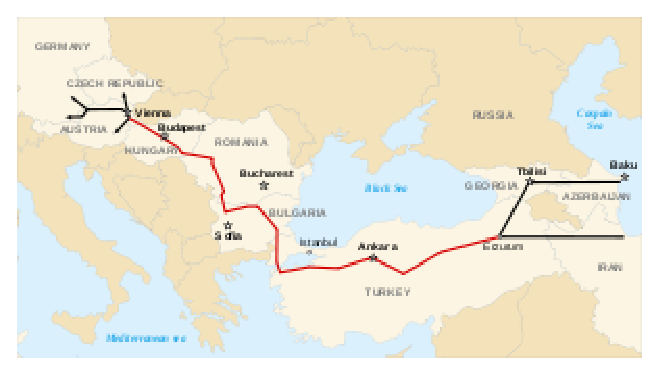
\epsfig{file=Nabucco.eps,height=\pos{4.5}{9}cm}
  \end{center}
    \caption{\brcolor{The Planned Nabucco Pipeline:}
    \pos{http://en.wikipedia.org/wiki/Nabucco\_Pipeline}{}}\label{pl.dia2} 
\end{figure}


\noindent
\begynd
\pind The Nabucco pipeline was, for many years, a planned pipeline
involving Austria, Turkey, Iran and other states and companies.
\afslut

\mnewfoil

\begin{figure}[ht]
  \begin{center}
  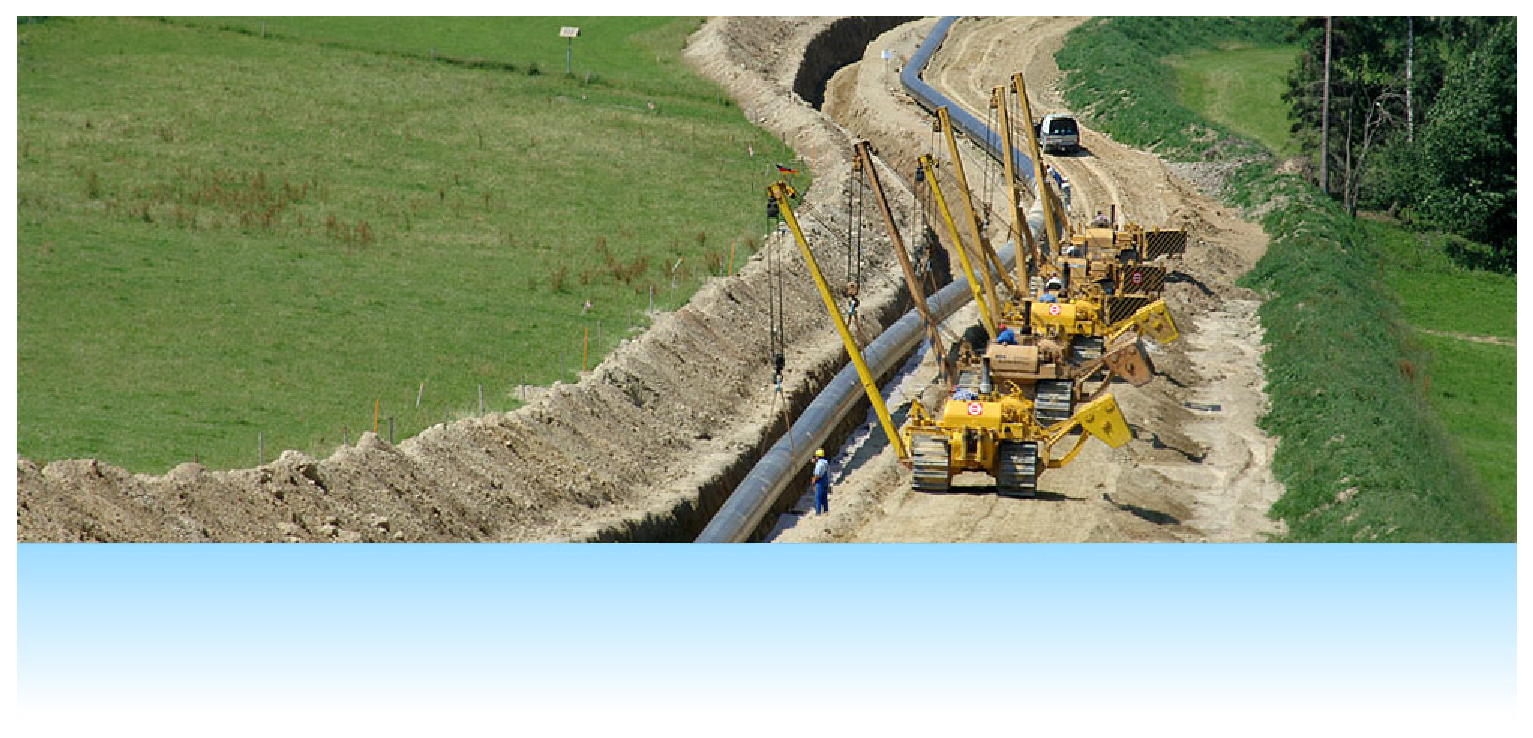
\epsfig{file=nabucco-digging,height=\pos{3.85}{11}cm}
  \end{center}
    \caption{\brcolor{Pipeline Construction}}\label{pl.dia3}
\end{figure}

\noindent
\begynd
\pind An example pipeline construction.
\pind It shows the linking of pipe segments.
\afslut
%\mnewfoil


\nbbbb{Pipes}

\begin{figure}[ht]
  \begin{center}
 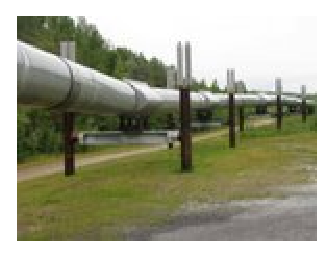
\epsfig{file=pipeline-1.eps,height=\pos{3.4}{6}cm}\ \ 
 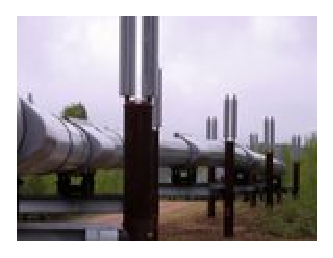
\epsfig{file=pipeline-2.eps,height=\pos{3.4}{6}cm}\ \ 
 
\epsfig{file=pipeline-3.eps,height=\pos{3.4}{6}cm}
  \end{center}
    \caption{\brcolor{Pipe Segments}}\label{pl.pipes}
 \end{figure}

\noindent
\begynd
\pind A pipe segment is a straight ``tube''-like unit.
\afslut
\nbbbb{Valves}
 
\begin{figure}[ht]
  \begin{center}
  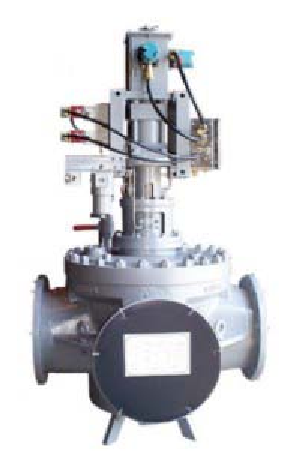
\epsfig{file=4Way-valve.eps,height=\pos{3.4}{6}cm}\ \ 
  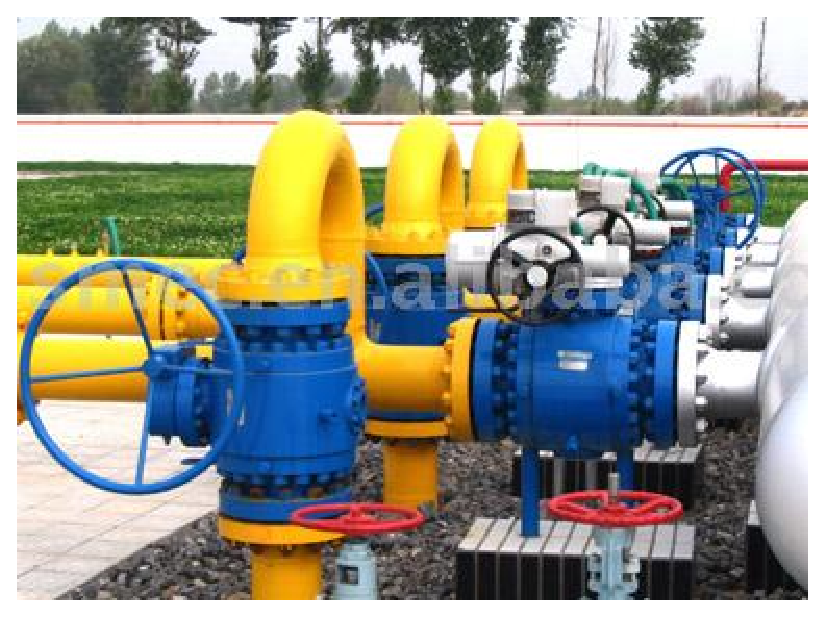
\epsfig{file=ball-valves.eps,height=\pos{3.4}{6}cm}\ \ 
  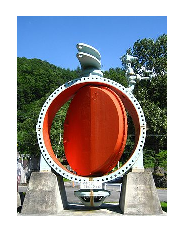
\epsfig{file=butterfly-valve-1.eps,height=\pos{3.4}{6}cm}\ \ 
  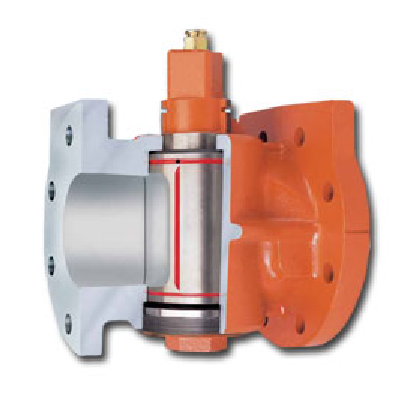
\epsfig{file=Resun-Plug-Valve.eps,height=\pos{3.4}{6}cm}
  \end{center}
    \caption{\brcolor{Valves}}\label{pl.valves}
 \end{figure}

\noindent
\begynd
\pind A pipe valve allows for the control of flow in pipes.
\afslut

\nbbbb{Pumps}
 
\begin{figure}[h]
  \begin{center}
      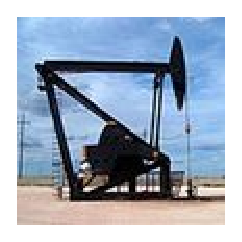
\epsfig{file=oil-drain-pump.eps,height=\pos{3.5}{7}cm}\ \ \ \ \
      \ \ \ \
      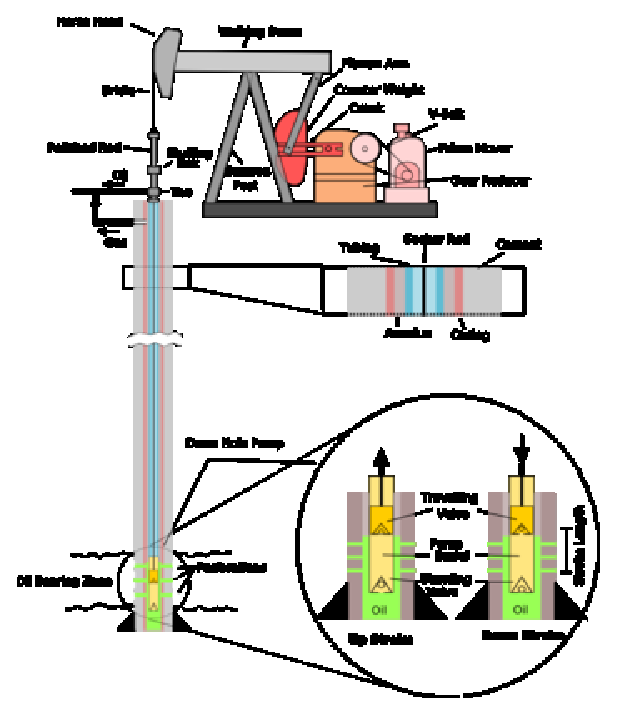
\epsfig{file=pump-jack.eps,height=\pos{3.5}{7}cm}
  \end{center}
    \caption{\brcolor{Oil Pumps}}\label{pl.pumps}
 \end{figure}

\noindent
\begynd
\pind A pump allows for the ``lifting'' of, for example, oil, over
      hilly terrain.
\pind The concept of \sfsl{pump head [height]} is relevant:
\begynd
\pind The \sfsl{head} is the height at which a pump can raise fluid up
      \nyl and is measured in meters or feet.
\afslut
\afslut

\nbbbb{Compressors}
 
\begin{figure}[h]
  \begin{center}
      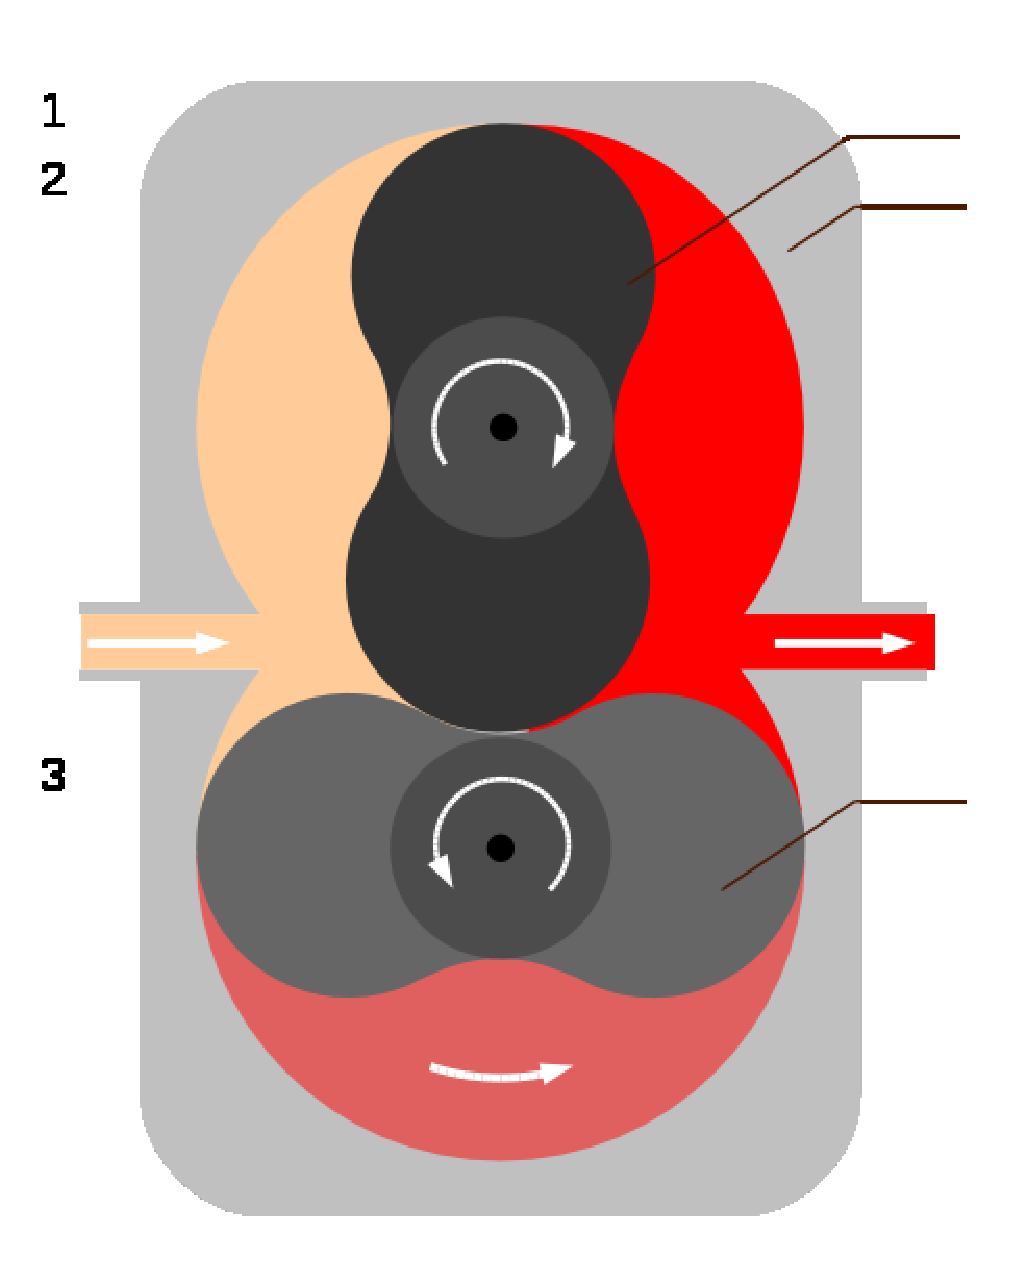
\epsfig{file=rotary-piston-pump.eps,height=\pos{3.4}{7}cm}\ \ \ 
      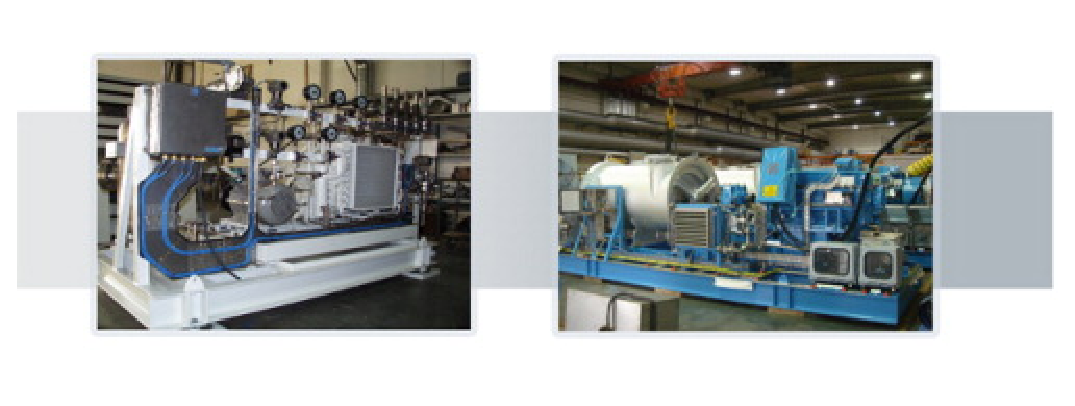
\epsfig{file=gas-compressor.eps,height=\pos{3.4}{7}cm}
  \end{center}
    \caption{\brcolor{Gas Compressors}}\label{pl.compressors}
 \end{figure}

\noindent
\begynd
\pind A compressor is used for gaseous liquids.
\begynd
\pind Compressors are similar to pumps: \nyl both increase the pressure on a fluid \nyl and both can transport the fluid through a pipe. \nyl As gases are compressible, \nyl the compressor also reduces the volume of a gas. 
\afslut
\afslut

\nbbbb{Pigs}
 
\begin{figure}[h]
  \begin{center}
  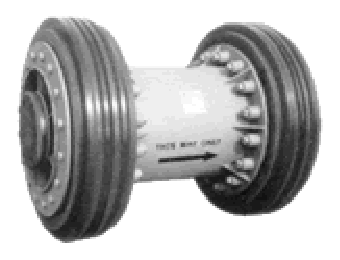
\epsfig{file=pig.eps,height=\pos{3.4}{7}cm}\ \ \ 
  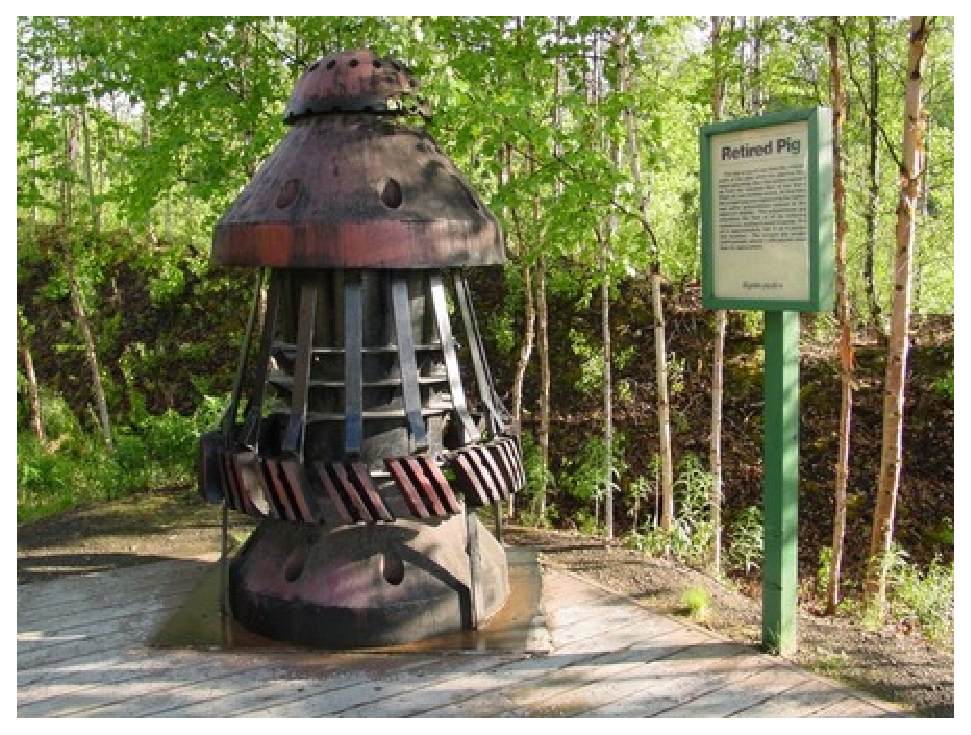
\epsfig{file=retired-pig.eps,height=\pos{3.4}{7}cm}
  \end{center}
    \caption{\brcolor{New and Old Pigs}}\label{pl.pig2} 
\end{figure}

\noindent
\begynd
\pind A ``pig'' is a tool that is sent down a pipeline and propelled
by the pressure of the product flow in the pipeline itself.  
\pind The primary purpose of pipeline pigs is to make sure that the
pipe is clean and free from obstruction.  
\afslut
\mnewfoil

\begin{figure}[h]
  \begin{center}
  
\epsfig{file=GasPigTrap.eps,height=\pos{3.4}{7}cm} \ \ 
  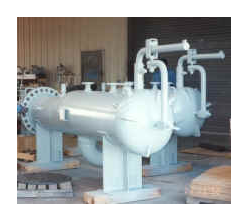
\epsfig{file=pig-receivers.eps,height=\pos{3.4}{7}cm}
  \end{center}
    \caption{\brcolor{Pig Launcher, Receiver}}\label{pl.pig1} 
 \end{figure}

\mnewfoil

\begin{figure}[ht]
  \begin{center}
    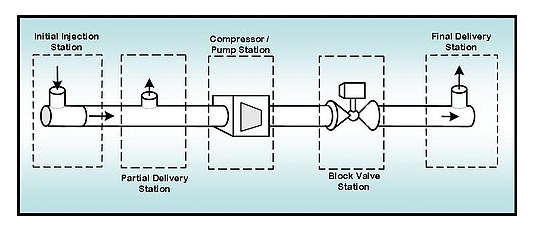
\epsfig{file=pipeline-diagram.eps,height=\pos{5}{8}cm}
    \caption{\brcolor{A Simple Pipeline}}\label{pi:pl.dia0}
  \end{center}
 \end{figure}

\noindent
\begynd
\pind Leftmost: A \sort{Well}. 
\pind 2nd from  left: a \sort{Fork}.
\pind Rightmost: a \sort{Sink}.
\afslut  
\mnewfoil

\begin{figure}[ht]
  \begin{center}
   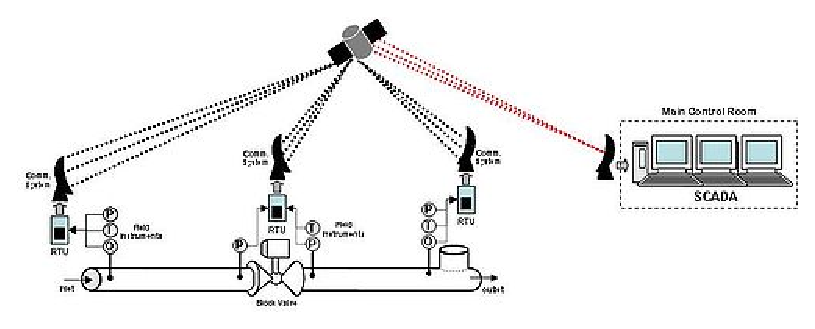
\epsfig{file=pipeline-scada.eps,height=\pos{5}{8}cm}
  \end{center}
    \caption{\brcolor{\LLLL\HHHH A Pipeline Monitoring \& Control System Diagram}}\label{pi:pl.dia1}
 \end{figure}

\noindent
\begynd
\pind Also called \sfsl{SCADA [Supervisory Control And Data Acquisition]}
\afslut 
%%  LocalWords:  Nabucco nd SCADA



\nbbbbb{Endurantes: Cualidades Externas}\label{pipe-ex1}\tehran{Endurants}{pipe:Edurants}\HHHH 

Seguimos la ontología de la Fig.\,\ref{anoipilisy}, el cuadro de líneas discontinuas de la izquierda
etiquetado como \sfsl{Cualidades Externas}.

\hDBfigure{onto}{\pos{10.8}{10}cm}{Ontología Superior}{anoipilisy}

\mnewfoil

\nbbbb{Partes}\tehran{Parts}{pipe:Parts}\HHHH

\DBfigure{opls-edin}{\pos{5}{10}cm}{Ejemplo de un sistema de tuberías}{nabucco}

\mnewfoil

\tehrantutorial{\begin{multicols}{2}}{}\HHHH
\begin{enumerate}\setei
\item \label{p-e-00} Un sistema de tuberías contiene un conjunto de unidades de tuberías y un monitor del sistema de tuberías.
\item \label{p-e--1} La buena formación de un sistema de tuberías
  depende de su mereología\pos{ (cf.\ sec.\,\ref{PLS Mereology})}{}
  y el enrutamiento de sus tuberías\pos{ (cf.\ sec.\,\ref{Wellformed Pipes})}{}. 
\item \label{p-e-01} Una unidad de tubería puede ser un pozo, una tubería, una bomba,
  una válvula, una bifurcación, una unión, una placa\footnote{\LLLL Una unidad de \sfsl{placa} es una
  placa de acero generalmente circular y plana utilizada para ``comenzar'' o ``terminar'' un
  segmento de tubería.}, o una unidad de desagüe.
\item \label{p-e-02} Consideramos todas estas unidades como
  distinguibles, es decir, el conjunto de pozos, el conjunto de tuberías, etc., el conjunto
  de desagües son disjuntos.
\savei\end{enumerate} 
\tehrantutorial{\end{multicols}}{}

\mnewfoil\LLLL
\tehrantutorial{\begin{multicols}{2}\footnotesize}{\LLLL}
\bp
\kw{type}\\
\ref{p-e-00}.\ \ PLS{\PRIM}, U, M \iptye{PLS$'$}{p-e-00}\iptye{U}{p-e-00}\iptye{M}{p-e-00}\\
\ref{p-e--1}.\ \ PLS {\EQ} {\LBRACE}{\BAR} pls:PLS{\PRIM}{\RDOT}wf\_PLS(pls) {\BAR}{\RBRACE} \iptye{PLS}{p-e--1} \\
\kw{value}\\
\ref{p-e--1}.\ \ wf\_PLS: PLS {\RIGHTARROW} \kw{Bool} \ipwf{wf\_PLS}{p-e--1}\\
\ref{p-e--1}.\ \ wf\_PLS(pls) {\IS}\\
\ref{p-e--1}.\ \ wf\_Mereology(pls){\WEDGE}wf\_Routes(pls){\WEDGE}wf\_Metrics(pls)\footnotemark\\
\ref{p-e-00}.\ \ obs\_Us: PLS {\RIGHTARROW} U\kw{-set} \ipob{obs\_Us}{p-e-00}\\
\ref{p-e-00}.\ \ obs\_M: PLS {\RIGHTARROW} M \ipob{obs\_M}{p-e-00}\\
\kw{type}\\
\ref{p-e-01}.\ \ U {\EQ} We {\BAR} Pi {\BAR} Pu {\BAR} Va {\BAR} Fo {\BAR} Jo {\BAR} Pl {\BAR} Si\iptye{U}{p-e-01}\\
\ref{p-e-02}.\ \ We :: Well\iptye{We}{p-e-02}\\
\ref{p-e-02}.\ \ Pi :: Pipe\iptye{Pi}{p-e-02} \\
\ref{p-e-02}.\ \ Pu :: Pump\iptye{Pu}{p-e-02} \\
\ref{p-e-02}.\ \ Va :: Valv\iptye{Va}{p-e-02}\\
\ref{p-e-02}.\ \ Fo :: Fork\iptye{Fo}{p-e-02}\\
\ref{p-e-02}.\ \ Jo :: Join\iptye{Jo}{p-e-02}\\
\ref{p-e-02}.\ \ Pl :: Plate\iptye{Pl}{p-e-02}\\
\ref{p-e-02}.\ \ Si :: Sink\iptye{Si}{p-e-02}
\ep
\tehrantutorial{\end{multicols}}{}
\footnotetext{\LLLL%
  \textsf{wf\_Mereology}, 
  \textsf{wf\_Routes} y
  \textsf{wf\_Metrics} se explicarán en las secciones\,%
  \vref{pipe:wfMereology},
  \vref{pipe:wfRoutes} y
  \vref{pipe:Wellformed Unit Metrics}.}


\nbbbb{Un Estado Endurante}

\begin{enumerate}\setei
\item \label{end-state-000} Para un sistema de tuberías dado % unsure how to make this flow well. The original english sentence is rather confusing.
\item \label{end-state-010} ejemplificamos un estado endurante $\sigma$
\item \label{end-state-020} compuesto del sistema de tuberías dado y
                            todas sus unidades manifiestas, es decir, sin placas.
\savei\end{enumerate}

\bp
\kw{value}\\
\ref{end-state-000}.\ \ \ pls:PLS\ \ \ipva{pls}{end-state-000}\\
\kw{variable}\\
\ref{end-state-010}.\ \ \ $\sigma$ :{\EQ} collect\_state(pls)\ \ \ipst{$\sigma$}{end-state-010} \\
\kw{value} \\
\ref{end-state-020}.\ \ \ collect\_state: PLS\ \ \ \ipfu{collect\_state}{end-state-020}\\
\ref{end-state-020}.\ \ \ collect\_state(pls) {\IS} {\LBRACE}pls{\RBRACE}\,{\UNION}\,obs\_Us(pls) {\SETMINUS} Pl
\ep

\nbbbbb{Endurantes: Cualidades Internas}

\begynd
\pind Seguimos la ontología de la fig.\,\vref{anoipilisy}, \nyl las
líneas verticales y horizontales de la izquierda.
\afslut


\bbbb{Identificación Única}

\begin{enumerate}\setei
\item \label{p-e-03z} El sistema de tuberías, como tal,
\item \label{p-e-03x} tiene un identificador único, distinto de sus
                      identificadores de unidades de tuberías. 
\item \label{p-e-03y} Cada unidad de tubería se distingue de manera única por
                      su identificador de unidad. 
\item \label{p-e-03zz} Existe un estado de todos los identificadores únicos.
\savei\end{enumerate}
\mnewfoil
%\RSLatex
%   type
%&\ref{p-e-03x}.&      PLSI &\iptyu{PLSI}{p-e-03x}&
%&\ref{p-e-03y}.&      UI &\iptyu{UI}{p-e-03y}&
%   value
%&\ref{p-e-03z}.&      pls:PLS
%&\ref{p-e-03x}.&      uid_PLS: PLS -> PLSI&\ipob{uid\_PLS}{p-e-03x}&
%&\ref{p-e-03y}.&      uid_U: U -> UI&\ipob{uid\_U}{p-e-03y}&
%   variable
%&\ref{p-e-03zz}.&      `sigma&$_{uid}$& := { uid_PLS(pls) } union xtr_UIs(pls) &\ipst{$\sigma_{uid}$}{p-e-03z}&
%   axiom &\ipax{Unique Identification}{p-e-03y}&
%&\ref{p-e-03y}.&      all u,u':U:-{u,u'}<<=obs_Us(pls)=>(u~=u'=>uid_UI(u)~=uid_UI(u'))
%&\ref{p-e-03y}.&    /\  uid_PLS(pls) ~isin {uid_UI(u)|u:U:-u isin obs_Us(pls)}
%\endRSLatex 
\bp
\>\ \kw{type}\\
\ref{p-e-03x}.\ \ \ \ \ \ PLSI \iptyu{PLSI}{p-e-03x}\\
\ref{p-e-03y}.\ \ \ \ \ \ UI \iptyu{UI}{p-e-03y}\\
\>\ \kw{value}\\
\ref{p-e-03z}.\ \ \ \ \ \ pls:PLS\\
\ref{p-e-03x}.\ \ \ \ \ \ uid\_PLS: PLS {\RIGHTARROW} PLSI\ipob{uid\_PLS}{p-e-03x}\\
\ref{p-e-03y}.\ \ \ \ \ \ uid\_U: U {\RIGHTARROW} UI\ipob{uid\_U}{p-e-03y}\\
\>\ \kw{variable}\\
\ref{p-e-03zz}.\ \ \ \ \ \ $\sigma$$_{uid}$ :{\EQ} {\LBRACE} uid\_PLS(pls) {\RBRACE} {\UNION} xtr\_UIs(pls) \ipst{$\sigma_{uid}$}{p-e-03z}\\
\>\ \kw{axiom} \ipax{Unique Identification}{p-e-03y}\\
\ref{p-e-03y}.\ \ \ \ \ \ {\ALL} u,u{\PRIM}:U{\RDOT}{\LBRACE}u,u{\PRIM}{\RBRACE}{\SUBSETEQ}obs\_Us(pls){\DBLRIGHTARROW}(u{\NOTEQ}u{\PRIM}{\DBLRIGHTARROW}uid\_UI(u){\NOTEQ}uid\_UI(u{\PRIM}))\\
\ref{p-e-03y}.\ \ \ \ {\WEDGE}\ \ uid\_PLS(pls) {\NOTISIN} {\LBRACE}uid\_UI(u){\BAR}u:U{\RDOT}u {\ISIN} obs\_Us(pls){\RBRACE}
\ep

\mnewfoil
\begin{enumerate}\setei
\item \label{p-e-03a} De un sistema de tuberías uno puede observar 
el conjunto de todos los identificadores únicos de unidades.
\savei\end{enumerate}


%\RSLatex
%   value
%&\ref{p-e-03a}.&   xtr_UIs: PLS -> UI-set&\ipfu{xtr\_UIs}{p-e-03a}&
%&\ref{p-e-03a}.&   xtr_UIs(pls) is {uid_UI(u)|u:U:-u isin obs_Us(pls)}
%\endRSLatex 
\bp
\>\ \kw{value}\\
\ref{p-e-03a}.\ \ \ xtr\_UIs: PLS {\RIGHTARROW} UI\kw{-set}\ipfu{xtr\_UIs}{p-e-03a}\\
\ref{p-e-03a}.\ \ \ xtr\_UIs(pls) {\IS} {\LBRACE}uid\_UI(u){\BAR}u:U{\RDOT}u {\ISIN} obs\_Us(pls){\RBRACE}
\ep

\begin{enumerate}\setei
\item \label{p-e-03b} Podemos demostrar que el número de identificadores
                      únicos de unidades es igual al número de unidades de ese sistema.
\savei\end{enumerate}


%\RSLatex
%   &\kw{theorem:}\ipth{Unique Endurants}{p-e-03b}&
%&\ref{p-e-03b}.&     all pls:PLS:-card obs_Us(pl)=card xtr_UIs(pls)
%\endRSLatex 
\bp
\>\ \kw{theorem:}\ipth{Endurantes Únicos}{p-e-03b}\\
\ref{p-e-03b}.\ \ \ \ \ {\ALL} pls:PLS{\RDOT}\kw{card} obs\_Us(pl){\EQ}\kw{card} xtr\_UIs(pls)
\ep

\nbbbb{Mereología}\label{PLS Mereology}\LLLL\HHHH

\bbb{Mereología PLS}

\item \label{pls-mer-00} La mereología de un sistema de tuberías es el 
  conjunto de identificadores únicos de todas las unidades del sistema.
\begin{enumerate}\setei
\savei\end{enumerate}

%\RSLatex
%type
%&\ref{pls-mer-00}.&   PLS_Mer = UI-set&\ipty{PLS\_Mer}{pls-mer-00}&
%value
%&\ref{pls-mer-00}.&   mereo_PLS: PLS -> PLS_Mer&\ipob{mereo\_PLS}{pls-mer-00}&
%axiom&\ipty{Wellformed Mereologies}{pls-mer-00}&
%&\ref{pls-mer-00}.&   all uis:PLS_Mer :- uis = card xtr_UIs(pls)
%\endRSLatex 
\bp
\kw{type}\\
\ref{pls-mer-00}.\ \ \ PLS\_Mer {\EQ} UI\kw{-set}\ipty{PLS\_Mer}{pls-mer-00}\\
\kw{value}\\
\ref{pls-mer-00}.\ \ \ mereo\_PLS: PLS {\RIGHTARROW} PLS\_Mer\ipob{mereo\_PLS}{pls-mer-00}\\
\kw{axiom}\ipty{Mereologías Bien Formadas}{pls-mer-00}\\
\ref{pls-mer-00}.\ \ \ {\ALL} uis:PLS\_Mer {\RDOT} uis {\EQ} \kw{card} xtr\_UIs(pls)
\ep

\nbbb{Mereologías de Unidades}\HHHH\LLLL

\begin{enumerate}\setei
\item \label{p-e-11}   Cada unidad está conectada a cero, una o dos
                       otras unidades de entrada existentes y a cero, una o dos
                       otras unidades de salida existentes como sigue:
\begin{enumerate}
\item \label{p-e-04}   Una unidad de pozo está conectada a exactamente una unidad de salida
                       (y, por lo tanto, no tiene ``entrada'').
\item \label{p-e-05}   Una unidad de tubería está conectada a exactamente una unidad de entrada
                       y una unidad de salida.
\item \label{p-e-06}   Una unidad de bomba está conectada a exactamente una unidad de entrada
                       y una unidad de salida.
\item \label{p-e-07}   Una válvula está conectada a exactamente una unidad de entrada
                       y una unidad de salida.
\item \label{p-e-08}   Una bifurcación está conectada a exactamente una unidad de entrada
                       y dos unidades de salida distintas.
\item \label{p-e-09}   Una unión está conectada a exactamente dos unidades de entrada distintas
                       y una unidad de salida.
\item \label{p-e-85}   Una placa está conectada a exactamente una unidad.
\item \label{p-e-10}   Un desagüe está conectado a exactamente una unidad de entrada
                       (y, por lo tanto, no tiene ``salida''). 
\end{enumerate}
\savei\end{enumerate}

\mnewfoil\LLLL

\bp
\>\ \kw{type}\\
\ref{p-e-11}.\ \ \ \ \ \ MER {\EQ} UI\kw{-set} {\TIMES} UI\kw{-set}\iptym{MER}{p-e-11}\\
\>\ \kw{value}\\
\ref{p-e-11}.\ \ \ \ \ \ mereo\_U: U {\RIGHTARROW} MER \ipob{mereo\_U}{p-e-11}\\
\>\ \kw{axiom}\\
\ref{p-e-11}.\ \ \ \ \ \ \ wf\_Mereology: PLS {\RIGHTARROW} \kw{Bool} \label{pipe:wfMereology}\ipwf{wf\_Mereology}{p-e-11}\\
\ref{p-e-11}.\ \ \ \ \ \ \ wf\_Mereology(pls) {\IS}\\
\ref{p-e-11}.\ \ \ \ \ \ \ \ \ \ {\ALL} u:U{\RDOT}u {\ISIN} obs\_Us(pls){\DBLRIGHTARROW} \\
\ref{p-e-11}.\ \ \ \ \ \ \ \ \ \ \ \ \ \kw{let} (iuis,ouis) {\EQ} mereo\_U(u) \kw{in} iuis {\UNION} ouis {\SUBSETEQ} xtr\_UIs(pls) {\WEDGE}\\
\ref{p-e-11}.\ \ \ \ \ \ \ \ \ \ \ \ \ \ \ \ \ \kw{case} (u,(\kw{card} uius,\kw{card} ouis)) \kw{of}\\
\ref{p-e-04}.\ \ \ \ \ \ \ \ \ \ \ \ \ \ \ \ \ \ \ \ \ (mk\_We(we),(0,1)) {\RIGHTARROW} \kw{true},\\
\ref{p-e-05}.\ \ \ \ \ \ \ \ \ \ \ \ \ \ \ \ \ \ \ \ \ (mk\_Pi(pi),(1,1)) {\RIGHTARROW} \kw{true},\\
\ref{p-e-06}.\ \ \ \ \ \ \ \ \ \ \ \ \ \ \ \ \ \ \ \ \ (mk\_Pu(pu),(1,1)) {\RIGHTARROW} \kw{true},\\
\ref{p-e-07}.\ \ \ \ \ \ \ \ \ \ \ \ \ \ \ \ \ \ \ \ \ (mk\_Va(va),(1,1)) {\RIGHTARROW} \kw{true},\\
\ref{p-e-08}.\ \ \ \ \ \ \ \ \ \ \ \ \ \ \ \ \ \ \ \ \ (mk\_Fo(fo),(1,1)) {\RIGHTARROW} \kw{true},\\
\ref{p-e-09}.\ \ \ \ \ \ \ \ \ \ \ \ \ \ \ \ \ \ \ \ \ (mk\_Jo(jo),(1,1)) {\RIGHTARROW} \kw{true},\\
\ref{p-e-09}.\ \ \ \ \ \ \ \ \ \ \ \ \ \ \ \ \ \ \ \ \ (mk\_Pl(pl),(0,1)) {\RIGHTARROW} \kw{true}, ``inicio''\\
\ref{p-e-09}.\ \ \ \ \ \ \ \ \ \ \ \ \ \ \ \ \ \ \ \ \ (mk\_Pl(pl),(1,0)) {\RIGHTARROW} \kw{true}, ``fin''\\
\ref{p-e-10}.\ \ \ \ \ \ \ \ \ \ \ \ \ \ \ \ \ \ \ \ \ (mk\_Si(si),(1,1)) {\RIGHTARROW} \kw{true},\\
\ref{p-e-11}.\ \ \ \ \ \ \ \ \ \ \ \ \ \ \ \ \ \ \ \ \ {\UNDERLINE} {\RIGHTARROW} \kw{false} \kw{end} \kw{end}
\ep

\nbbbb{Conceptos de Tuberías, I}

\bbb{Rutas de Tuberías}\label{primer-pipe}\HHHH

\begin{enumerate}\setei
\item \label{p-e-12} Una ruta (de un sistema de tuberías) es una secuencia de
                     unidades conectadas (del sistema de tuberías).
\item \label{p-e-13} Un descriptor de ruta es una secuencia de identificadores de unidades
                     y las unidades conectadas de una ruta
                     (de un sistema de tuberías).
\savei\end{enumerate}

\bp
\>\ \kw{type}\\
\ref{p-e-12}.\ \ \ \ \ \ R{\PRIM} {\EQ} U$^{\omega}$ \iptyo{R$'$}{p-e-12}\\
\ref{p-e-12}.\ \ \ \ \ \ R {\EQ} {\LBRACE}{\BAR} r:Route{\PRIM}{\RDOT}wf\_Route(r) {\BAR}{\RBRACE} \iptyo{R}{p-e-12}\\
\ref{p-e-13}.\ \ \ \ \ \ RD {\EQ} UI$^{\omega}$ \iptyo{RD}{p-e-13}\\
\>\ \kw{axiom}\\
\ref{p-e-13}.\ \ \ \ \ \ {\ALL} rd:RD {\RDOT} {\EXISTS} r:R{\RDOT}rd{\EQ}descriptor(r) \ipax{Describibilidad de Rutas}{p-e-13}\\
\>\ \kw{value}\\
\ref{p-e-13}.\ \ \ \ \ \ descriptor: R {\RIGHTARROW} RD \ipfu{descriptor}{p-e-13}\\
\ref{p-e-13}.\ \ \ \ \ \ descriptor(r) {\IS} {\LANGLE}uid\_UI(r{\LBRACKET}i{\RBRACKET}){\BAR}i:\kw{Nat}{\RDOT}1{\LEQ}i{\LEQ}\kw{len} r{\RANGLE}\ \ \ 
\ep

\mnewfoil\LLLL\HHHH

\begin{enumerate}\setei
\item \label{p-e-20x}   Dos unidades son adyacentes si los identificadores de unidades de salida
  de una comparten un identificador de unidad único con los identificadores de entrada
  de la otra.
\savei\end{enumerate}

\bp
\>\ \kw{value} \\
\ref{p-e-20x}.\ \ \ \ \ \ adjacent: U {\TIMES} U {\RIGHTARROW} \kw{Bool} \ipfu{adjacent}{p-e-20x}\\
\ref{p-e-20x}.\ \ \ \ \ \ adjacent(u,u{\PRIM}) {\IS} \kw{let} (,ouis){\EQ}mereo\_U(u),(iuis,){\EQ}mereo\_U(u{\PRIM}) \kw{in} ouis {\INTER} iuis {\NOTEQ} {\LBRACE}{\RBRACE} \kw{end}
\ep

\LLLL

\begin{enumerate}\setei
\item \label{p-e-20a}   Dado un sistema de tuberías, $pls$, se puede identificar el
                  (posiblemente infinito) conjunto de rutas (posiblemente infinitas)
                  de ese sistema de tuberías.
\begin{enumerate}
\item \label{p-e-20}  La secuencia vacía, {\LANGLE}{\RANGLE}, es una
                      ruta de $pls$.  
\item \label{p-e-21}  Sea $u, u'$ cualquier unidad de $pls$, tal que
                      un identificador de unidad de salida de $u$ sea el mismo que
                      un identificador de unidad de entrada de $u'$, entonces
                      {\LANGLE}$u,u'${\RANGLE} es una ruta de $pls$.
\item \label{p-e-22}  Si $r$ y $r'$ son rutas de $pls$ tal que
                      el último elemento de $r$ es el mismo que el primer
                      elemento de $r'$, entonces $r${\CONCAT}\kw{tl}$r'$ es
                      una ruta de $pls$.  
\item \label{p-e-23}  Ninguna secuencia de unidades es una ruta a menos que
                      se siga de un número finito (o infinito) de
                      aplicaciones de las cláusulas base e inductivas
                      de los artículos~\ref{p-e-20}--\ref{p-e-22}.
\end{enumerate}
\savei\end{enumerate}

\mnewfoil\LLLL\HHHH

%\RSLatex 
%   value
%&\ref{p-e-20a}.&      Routes: PLS -> RD-infset&\ipfu{Routes}{p-e-20a}&
%&\ref{p-e-20a}.&      Routes(pls) is 
%&\ref{p-e-20}.&          let rs = <..> union 
%&\ref{p-e-21}.&                   {<.uid_UI(u),uid_UI(u').>|u,u':U:-{u,u'}<<=obs_Us(pls) /\ adjacent(u,u')}
%&\ref{p-e-22}.&                 union {r^tl r'|r,r':R:-{r,r'}<<=rs}
%&\ref{p-e-23}.&          in rs end
%\endRSLatex 
\bp
\>\ \kw{value}\\
\ref{p-e-20a}.\ \ \ \ \ \ Routes: PLS {\RIGHTARROW} RD\kw{-infset}\ipfu{Routes}{p-e-20a}\\
\ref{p-e-20a}.\ \ \ \ \ \ Routes(pls) {\IS} \\
\ref{p-e-20}.\ \ \ \ \ \ \ \ \ \ \kw{let} rs {\EQ} {\LANGLE}{\RANGLE} {\UNION} \\
\ref{p-e-21}.\ \ \ \ \ \ \ \ \ \ \ \ \ \ \ \ \ \ \ {\LBRACE}{\LANGLE}uid\_UI(u),uid\_UI(u{\PRIM}){\RANGLE}{\BAR}u,u{\PRIM}:U{\RDOT}{\LBRACE}u,u{\PRIM}{\RBRACE}{\SUBSETEQ}obs\_Us(pls) {\WEDGE} adjacent(u,u{\PRIM}){\RBRACE}\\
\ref{p-e-22}.\ \ \ \ \ \ \ \ \ \ \ \ \ \ \ \ \ {\UNION} {\LBRACE}r{\CONCAT}\kw{tl} r{\PRIM}{\BAR}r,r{\PRIM}:R{\RDOT}{\LBRACE}r,r{\PRIM}{\RBRACE}{\SUBSETEQ}rs{\RBRACE}\\
\ref{p-e-23}.\ \ \ \ \ \ \ \ \ \ \kw{in} rs \kw{end}
\ep

\bbb{Well-formed Routes}\label{Wellformed Pipes}

\begin{enumerate}\setei
\item \label{p-e-14a}  A route is acyclic if no two route positions
  reveal the same unique unit identifier.
\savei\end{enumerate}
%\RSLatex
%   value
%&\ref{p-e-14a}.&   is_acyclic_Route: R -> Bool&\ippr{is\_acyclic\_Route}{p-e-14a}&
%&\ref{p-e-14a}.&   is_acyclic_Route(r) is ~exists i,j:Nat:-{i,j}<<=inds r /\ i~=j /\ r[i]=r[j]
%\endRSLatex 
\bp
\>\ \kw{value}\\
\ref{p-e-14a}.\ \ \ is\_acyclic\_Route: R {\RIGHTARROW} \kw{Bool}\ippr{is\_acyclic\_Route}{p-e-14a}\\
\ref{p-e-14a}.\ \ \ is\_acyclic\_Route(r) {\IS} {\SIM}{\EXISTS} i,j:\kw{Nat}{\RDOT}{\LBRACE}i,j{\RBRACE}{\SUBSETEQ}\kw{inds} r {\WEDGE} i{\NOTEQ}j {\WEDGE} r{\LBRACKET}i{\RBRACKET}{\EQ}r{\LBRACKET}j{\RBRACKET}
\ep

\mnewfoil

\begin{enumerate}\setei
\item \label{p-e-14b}  A pipeline system is well-formed if none of its
                      routes are circular (and all of its routes
                      embedded in well-to-sink routes). 
\savei\end{enumerate}
%\RSLatex
%   value
%&\ref{p-e-14b}.&   wf_Routes: PLS -> Bool&\ipwf{wf\_Routes}{p-e-14b}&
%&\ref{p-e-14b}.&   wf_Routes(pls) is  &\label{pipe:wfRoutes}&
%&\ref{p-e-14b}.&       non_circular(pls) /\ are_embedded_Routes(pls)
%
%&\ref{p-e-14b}.&   is_non_circular_PLS: PLS -> Bool&\ipwf{is\_non\_circular\_PLS}{p-e-14b}&
%&\ref{p-e-14b}.&   is_non_circular_PLS(pls) is 
%&\ref{p-e-14b}.&       all r:R:-r isin routes(p)/\acyclic_Route(r)
%\endRSLatex 
\bp
\>\ \kw{value}\\
\ref{p-e-14b}.\ \ \ wf\_Routes: PLS {\RIGHTARROW} \kw{Bool}\ipwf{wf\_Routes}{p-e-14b}\\
\ref{p-e-14b}.\ \ \ wf\_Routes(pls) {\IS}\ \ \label{pipe:wfRoutes}\\
\ref{p-e-14b}.\ \ \ \ \ \ \ non\_circular(pls) {\WEDGE} are\_embedded\_Routes(pls)\\
\\
\ref{p-e-14b}.\ \ \ is\_non\_circular\_PLS: PLS {\RIGHTARROW} \kw{Bool}\ipwf{is\_non\_circular\_PLS}{p-e-14b}\\
\ref{p-e-14b}.\ \ \ is\_non\_circular\_PLS(pls) {\IS} \\
\ref{p-e-14b}.\ \ \ \ \ \ \ {\ALL} r:R{\RDOT}r {\ISIN} routes(p){\WEDGE}acyclic\_Route(r)
\ep

\mnewfoil

\begin{enumerate}\setei
\item \label{p-e-19}  We define well-formedness in terms of
  well-to-sink routes, i.e., routes which start with a well unit and
  end with a sink unit.
\savei\end{enumerate}

%\RSLatex
%   value   
%&\ref{p-e-19}.&   well_to_sink_Routes: PLS -> R-set&\ipfu{well\_to\_sink\_Routes}{p-e-19}&
%&\ref{p-e-19}.&   well_to_sink_Routes(pls) is
%&\ref{p-e-19}.&      let rs = Routes(pls) in
%&\ref{p-e-19}.&      {r|r:R:-r isin rs /\ is_We(r[1]) /\ is_Si(r[len r])} end
%\endRSLatex 
\bp
\>\ \kw{value}\ \ \ \\
\ref{p-e-19}.\ \ \ well\_to\_sink\_Routes: PLS {\RIGHTARROW} R\kw{-set}\ipfu{well\_to\_sink\_Routes}{p-e-19}\\
\ref{p-e-19}.\ \ \ well\_to\_sink\_Routes(pls) {\IS}\\
\ref{p-e-19}.\ \ \ \ \ \ \kw{let} rs {\EQ} Routes(pls) \kw{in}\\
\ref{p-e-19}.\ \ \ \ \ \ {\LBRACE}r{\BAR}r:R{\RDOT}r {\ISIN} rs {\WEDGE} is\_We(r{\LBRACKET}1{\RBRACKET}) {\WEDGE} is\_Si(r{\LBRACKET}\kw{len} r{\RBRACKET}){\RBRACE} \kw{end}
\ep

\mnewfoil

\begin{enumerate}\setei
\item \label{p-e-18} A pipeline system is well-formed
      if all of its routes are embedded in well-to-sink routes.
\savei\end{enumerate}

%\RSLatex
%&\ref{p-e-18}.&   are_embedded_Routes: PLS -> Bool&\ippr{are\_embedded\_Routes}{p-e-18}&
%&\ref{p-e-18}.&   are_embedded_Routes(pls) is   
%&\ref{p-e-18}.&       let wsrs = well_to_sink_Routes(pls) in
%&\ref{p-e-18}.&       all r:R :- r isin Routes(pls) =>
%&\ref{p-e-18}.&           exists r':R,i,j:Nat :- 
%&\ref{p-e-18}.&              r' isin wsrs /\ {i,j}<<=inds r'/\i<=j /\ r = <.r'[k]|k:Nat:-i<=k<=j.> end
%\endRSLatex 
\bp
\ref{p-e-18}.\ \ \ are\_embedded\_Routes: PLS {\RIGHTARROW} \kw{Bool}\ippr{are\_embedded\_Routes}{p-e-18}\\
\ref{p-e-18}.\ \ \ are\_embedded\_Routes(pls) {\IS}\ \ \ \\
\ref{p-e-18}.\ \ \ \ \ \ \ \kw{let} wsrs {\EQ} well\_to\_sink\_Routes(pls) \kw{in}\\
\ref{p-e-18}.\ \ \ \ \ \ \ {\ALL} r:R {\RDOT} r {\ISIN} Routes(pls) {\DBLRIGHTARROW}\\
\ref{p-e-18}.\ \ \ \ \ \ \ \ \ \ \ {\EXISTS} r{\PRIM}:R,i,j:\kw{Nat} {\RDOT} \\
\ref{p-e-18}.\ \ \ \ \ \ \ \ \ \ \ \ \ \ r{\PRIM} {\ISIN} wsrs {\WEDGE} {\LBRACE}i,j{\RBRACE}{\SUBSETEQ}\kw{inds} r{\PRIM}{\WEDGE}i{\LEQ}j {\WEDGE} r {\EQ} {\LANGLE}r{\PRIM}{\LBRACKET}k{\RBRACKET}{\BAR}k:\kw{Nat}{\RDOT}i{\LEQ}k{\LEQ}j{\RANGLE} \kw{end}
\ep

\bbb{Embedded Routes}

\begin{enumerate}\setei
\item \label{p-e-33a} For every route we can define the set of all its
                      embedded routes. 
\savei\end{enumerate} 

%\RSLatex
%   value
%&\ref{p-e-33a}.&  embedded_Routes: R -> R-set&\ipfu{embedded\_Routes}{p-e-33a}&
%&\ref{p-e-33a}.&  embedded_Routes(r) is {<.r[k]|k:Nat:-i<=k<=j.> | i,j:Nat:- i {i,j}<<=inds(r) /\ i<=j}  
%\endRSLatex 
\bp
\>\ \kw{value}\\
\ref{p-e-33a}.\ \ embedded\_Routes: R {\RIGHTARROW} R\kw{-set}\ipfu{embedded\_Routes}{p-e-33a}\\
\ref{p-e-33a}.\ \ embedded\_Routes(r) {\IS} {\LBRACE}{\LANGLE}r{\LBRACKET}k{\RBRACKET}{\BAR}k:\kw{Nat}{\RDOT}i{\LEQ}k{\LEQ}j{\RANGLE} {\BAR} i,j:\kw{Nat}{\RDOT} i {\LBRACE}i,j{\RBRACE}{\SUBSETEQ}\kw{inds}(r) {\WEDGE} i{\LEQ}j{\RBRACE}\ \ 
\ep

\nbbb{A Theorem}

\begin{enumerate}\setei
\item \label{p-e-33b} The following theorem is conjectured:
\begin{enumerate}
\item \label{p-e-30}  the set of all routes  (of the pipeline system)
\item \label{p-e-31}  is the set of all well-to-sink routes (of a
                      pipeline system) and 
\item \label{p-e-32}  all their embedded routes
\end{enumerate}
\savei\end{enumerate}

%\RSLatex
%   &\kw{theorem:}\ipth{Routes of a PLS}{p-e-33b}&
%&\ref{p-e-33b}.&   all pls:PLS :-
%&\ref{p-e-33b}.&   let rs = Routes(pls),
%&\ref{p-e-33b}.&       wsrs = well_to_sink_Routes(pls) in
%&\ref{p-e-30}.&   rs = 
%&\ref{p-e-31}.&        wsrs union
%&\ref{p-e-32}.&        union {{r'|r':R :- r' isin is_embedded_Routes(r'')} | r'':R :- r'' isin wsrs}
%&\ref{p-e-33a}.&   end
%\endRSLatex 
\bp
\>\ \kw{theorem:}\ipth{Routes of a PLS}{p-e-33b}\\
\ref{p-e-33b}.\ \ \ {\ALL} pls:PLS {\RDOT}\\
\ref{p-e-33b}.\ \ \ \kw{let} rs {\EQ} Routes(pls),\\
\ref{p-e-33b}.\ \ \ \ \ \ \ wsrs {\EQ} well\_to\_sink\_Routes(pls) \kw{in}\\
\ref{p-e-30}.\ \ \ rs {\EQ} \\
\ref{p-e-31}.\ \ \ \ \ \ \ \ wsrs {\UNION}\\
\ref{p-e-32}.\ \ \ \ \ \ \ \ {\UNION} {\LBRACE}{\LBRACE}r{\PRIM}{\BAR}r{\PRIM}:R {\RDOT} r{\PRIM} {\ISIN} is\_embedded\_Routes(r{\PRIM}{\PRIM}){\RBRACE} {\BAR} r{\PRIM}{\PRIM}:R {\RDOT} r{\PRIM}{\PRIM} {\ISIN} wsrs{\RBRACE}\\
\ref{p-e-33a}.\ \ \ \kw{end}
\ep

\nbbb{Fluids}

\begin{enumerate}\setei
\item \label{p-e-34} The only fluid of concern to pipelines is the
                     gas\footnote{\LLLL Gaseous materials include: air, gas,
                     etc.} or liquid\footnote{\LLLL Liquid materials include
                     water, oil, etc.} which the pipes
                     transport\footnote{\LLLL The description of this
                     document is relevant only to gas or oil pipelines.}.
\savei\end{enumerate}

%\RSLatex
%   type
%&\ref{p-e-34}.&      GoL [ = M ] &\iptye{GoL}{p-e-34}&
%   value
%&\ref{p-e-34}.&      obs_GoL: U -> GoL&\ipob{obs\_GoL}{p-e-34}&  
%\endRSLatex 
\bp
\>\ \kw{type}\\
\ref{p-e-34}.\ \ \ \ \ \ GoL {\LBRACKET} {\EQ} M {\RBRACKET} \iptye{GoL}{p-e-34}\\
\>\ \kw{value}\\
\ref{p-e-34}.\ \ \ \ \ \ obs\_GoL: U {\RIGHTARROW} GoL\ipob{obs\_GoL}{p-e-34}\ \ 
\ep

\nbbbb{Attributes}\LLLL

\bbb{Unit Flow Attributes}\HHHH


\begin{enumerate}\setei
\item A number of attribute types characterise units:
\begin{enumerate}
\item \label{pa01x} estimated current well capacity (barrels of oil, etc.),
\item \label{pa03x} pump height (a static attribute), 
\item \label{pa04x} current pump status (not pumping, pumping; a programmable attribute),
\item \label{pa05x} current valve status (closed, open; a programmable attribute) and
\item \label{pa06x} flow (barrels/second, a biddable attribute).
\end{enumerate}
\savei\end{enumerate}

\mnewfoil\LLLL\HHHH%&$_{\mathcall{L}}$&

%\begin{multicols}{2}
%\RSLatex
%   type
%&\ref{pa01x}.&      WellCap &\iptya{WellCap}{pa01x}&
%&\ref{pa03x}.&      Pump_Height &\iptya{Pump\_Height}{pa03x}&
%&\ref{pa04x}.&      Pump_State == {|&\sort{not\_pumping}&,&\sort{pumping}&|} &\iptya{Pump\_State}{pa04x}&
%&\ref{pa05x}.&      Valve_State == {|&\sort{closed}&,&\sort{open}&|} &\iptya{Valve\_State}{pa05x}&
%&\ref{pa06x}.&      Flow &\iptya{Flow}{pa06x}&
%\endRSLatex 
\bp
\>\ \kw{type}\\
\ref{pa01x}.\ \ \ \ \ \ WellCap \iptya{WellCap}{pa01x}\\
\ref{pa03x}.\ \ \ \ \ \ Pump\_Height \iptya{Pump\_Height}{pa03x}\\
\ref{pa04x}.\ \ \ \ \ \ Pump\_State {\EQ}{\EQ} {\LBRACE}{\BAR}\sort{not\_pumping},\sort{pumping}{\BAR}{\RBRACE} \iptya{Pump\_State}{pa04x}\\
\ref{pa05x}.\ \ \ \ \ \ Valve\_State {\EQ}{\EQ} {\LBRACE}{\BAR}\sort{closed},\sort{open}{\BAR}{\RBRACE} \iptya{Valve\_State}{pa05x}\\
\ref{pa06x}.\ \ \ \ \ \ Flow \iptya{Flow}{pa06x}
\ep
\begin{enumerate}\setei
\item \label{pa05y1} Flows can be added and subtracted,
\item \label{pa05y2} added distributively  and
\item \label{pa05z} flows can be compared.
\savei\end{enumerate}

%\RSLatex
%   value
%&\ref{pa05y1}.&      &$\oplus,\ominus$&: Flow><Flow -> Flow &\ipop{$\oplus$}{pa05y1}\ipop{$\ominus$}{pa05y1}&
%&\ref{pa05y2}.&      &$\oplus$&: Flow-set -> Flow  &\ipop{$\oplus$}{pa05y2}&
%&\ref{pa05z}.&      <,<=,=,~=,>=,>: Flow >< Flow -> Bool
%\endRSLatex 
\bp
\>\ \kw{value}\\
\ref{pa05y1}.\ \ \ \ \ \ $\oplus,\ominus$: Flow{\TIMES}Flow {\RIGHTARROW} Flow \ipop{$\oplus$}{pa05y1}\ipop{$\ominus$}{pa05y1}\\
\ref{pa05y2}.\ \ \ \ \ \ $\oplus$: Flow\kw{-set} {\RIGHTARROW} Flow\ \ \ipop{$\oplus$}{pa05y2}\\
\ref{pa05z}.\ \ \ \ \ \ {\LT},{\LEQ},{\EQ},{\NOTEQ},{\GEQ},{\GT}: Flow {\TIMES} Flow {\RIGHTARROW} \kw{Bool}
\ep
\ipop{\LT}{pa05z}%
\ipop{\LEQ}{pa05z}%
\ipop{\EQ}{pa05z}%
\ipop{\NOTEQ}{pa05z}%
\ipop{\GEQ}{pa05z}%
\ipop{\GT}{pa05z}
\mnewfoil
\begin{enumerate}\setei
\item \label{pa00} Properties of pipeline units include
%%%\begin{multicols}{2}
\begin{enumerate}
\item \label{pa01} estimated current well capacity (barrels of oil,
  etc.) [a biddable attribute], 
\item \label{pa02} pipe length [a static attribute],
\item \label{pa03} current pump height [a biddable attribute], 
\item \label{pa04} current valve open/close status [a programmable attribute],
\item \label{pa05} current [$\mathcal{L}$aminar] in-flow at unit input
                   [a monitorable attribute],
\item \label{pa06} current $\mathcal{L}$aminar] in-flow leak at unit input
                   [a monitorable attribute],
\item \label{pa07} maximum [$\mathcal{L}$aminar] guaranteed in-flow leak at unit input
  [a static attribute],
\mnewfoil
\item \label{pa08} current [$\mathcal{L}$aminar] leak unit interior
                   [a monitorable attribute],
\item \label{pa09} current [$\mathcal{L}$aminar] flow in unit interior
                   [a monitorable attribute],
\item \label{pa10} maximum $\mathcal{L}$aminar] guaranteed flow in unit interior
                   [a monitorable attribute],
\item \label{pa11} current [$\mathcal{L}$aminar] out-flow at unit output
                   [a monitorable attribute],
\item \label{pa12} current [$\mathcal{L}$aminar] out-flow leak at unit output
                   [a monitorable attribute] and
\item \label{pa13} maximum guaranteed $\mathcal{L}$aminar out-flow leak at unit output
                   [a static attribute.
\end{enumerate}
%%%\end{multicols}
\savei\end{enumerate}
\mnewfoil
\begin{multicols}{2}\LLLL
%\RSLatex
%type 
%&\ref{pa05}&  In_Flow = Flow&\iptya{In\_Flow}{pa05}&
%&\ref{pa06}&  In_Leak = Flow&\iptya{In\_Leak}{pa06}&
%&\ref{pa07}&  Max_In_Leak = Flow&\iptya{Max\_In\_Leak}{pa07}&
%&\ref{pa08}&  Body_Flow = Flow&\iptya{Body\_Flow}{pa08}&
%&\ref{pa09}&   Body_Leak = Flow&\iptya{Body\_Leak}{pa09}&
%&\ref{pa10}&   Max_Flow = Flow&\iptya{Max\_Flow}{pa10}&
%&\ref{pa11}&  Out_Flow = Flow&\iptya{Out\_Flow}{pa11}&
%&\ref{pa12}&   Out_Leak = Flow&\iptya{Out\_Leak}{pa12}& 
%&\ref{pa13}&  Max_Out_Leak = Flow&\iptya{Max\_Out\_Leak}{pa13}&
%value
%&\ref{pa01}&  attr_WellCap: We -> WellCap    
%&\ref{pa02}&  attr_LEN: Pi -> LEN   
%&\ref{pa03}&  attr_Height: Pu -> Height
%&\ref{pa04}&  attr_ValSta: Va -> VaSta
%&\ref{pa05}&  attr_In_Flow: U -> UI -> Flow&\ipob{attr\_In\_Flow}{pa05}&
%&\ref{pa06}&  attr_In_Leak: U -> UI -> Flow &\ipob{attr\_In\_Leak}{pa06}&  
%&\ref{pa07}&  attr_Max_In_Leak: U -> UI -> Flow &\ipob{attr\_Max\_In\_Leak}{pa07}&  
%&\ref{pa08}&  attr_Body_Flow: U -> Flow &\ipob{attr\_Body\_Flow}{pa08}&    
%&\ref{pa09}&   attr_Body_Leak: U -> Flow  &\ipob{attr\_Body\_Leak}{pa09}&
%&\ref{pa10}&   attr_Max_Flow: U -> Flow  &\ipob{attr\_Max\_Flow}{pa10}&
%&\ref{pa11}&  attr_Out_Flow: U -> UI -> Flow  &\ipob{attr\_Out\_Flow}{pa11}&
%&\ref{pa12}&   attr_Out_Leak: U -> UI -> Flow &\ipob{attr\_Out\_Leak}{pa12}& 
%&\ref{pa13}&  attr_Max_Out_Leak: U -> UI -> Flow&\ipob{attr\_Max\_Out\_Leak}{pa13}&
%\endRSLatex 
\bp
\kw{type} \\
\ref{pa05}\ \ In\_Flow {\EQ} Flow\iptya{In\_Flow}{pa05}\\
\ref{pa06}\ \ In\_Leak {\EQ} Flow\iptya{In\_Leak}{pa06}\\
\ref{pa07}\ \ Max\_In\_Leak {\EQ} Flow\iptya{Max\_In\_Leak}{pa07}\\
\ref{pa08}\ \ Body\_Flow {\EQ} Flow\iptya{Body\_Flow}{pa08}\\
\ref{pa09}\ \ \ Body\_Leak {\EQ} Flow\iptya{Body\_Leak}{pa09}\\
\ref{pa10}\ \ \ Max\_Flow {\EQ} Flow\iptya{Max\_Flow}{pa10}\\
\ref{pa11}\ \ Out\_Flow {\EQ} Flow\iptya{Out\_Flow}{pa11}\\
\ref{pa12}\ \ \ Out\_Leak {\EQ} Flow\iptya{Out\_Leak}{pa12} \\
\ref{pa13}\ \ Max\_Out\_Leak {\EQ} Flow\iptya{Max\_Out\_Leak}{pa13}\\
\kw{value}\\
\ref{pa01}\ \ attr\_WellCap: We {\RIGHTARROW} WellCap\ \ \ \ \\
\ref{pa02}\ \ attr\_LEN: Pi {\RIGHTARROW} LEN\ \ \ \\
\ref{pa03}\ \ attr\_Height: Pu {\RIGHTARROW} Height\\
\ref{pa04}\ \ attr\_ValSta: Va {\RIGHTARROW} VaSta\\
\ref{pa05}\ \ attr\_In\_Flow: U {\RIGHTARROW} UI {\RIGHTARROW} Flow\ipob{attr\_In\_Flow}{pa05}\\
\ref{pa06}\ \ attr\_In\_Leak: U {\RIGHTARROW} UI {\RIGHTARROW} Flow \ipob{attr\_In\_Leak}{pa06}\ \ \\
\ref{pa07}\ \ attr\_Max\_In\_Leak: U {\RIGHTARROW} UI {\RIGHTARROW} Flow \ipob{attr\_Max\_In\_Leak}{pa07}\ \ \\
\ref{pa08}\ \ attr\_Body\_Flow: U {\RIGHTARROW} Flow \ipob{attr\_Body\_Flow}{pa08}\ \ \ \ \\
\ref{pa09}\ \ \ attr\_Body\_Leak: U {\RIGHTARROW} Flow\ \ \ipob{attr\_Body\_Leak}{pa09}\\
\ref{pa10}\ \ \ attr\_Max\_Flow: U {\RIGHTARROW} Flow\ \ \ipob{attr\_Max\_Flow}{pa10}\\
\ref{pa11}\ \ attr\_Out\_Flow: U {\RIGHTARROW} UI {\RIGHTARROW} Flow\ \ \ipob{attr\_Out\_Flow}{pa11}\\
\ref{pa12}\ \ \ attr\_Out\_Leak: U {\RIGHTARROW} UI {\RIGHTARROW} Flow \ipob{attr\_Out\_Leak}{pa12} \\
\ref{pa13}\ \ attr\_Max\_Out\_Leak: U {\RIGHTARROW} UI {\RIGHTARROW} Flow\ipob{attr\_Max\_Out\_Leak}{pa13}
\ep
\end{multicols}

\mnewfoil\HHHH
\begin{enumerate}\setei
\item \label{pa13xy} Summarising we can define a two notions of flow:
\begin{enumerate}
\item \label{pa13x} static and
\item \label{pa13xz} monitorable.
\savei\end{enumerate}
\savei\end{enumerate}\footnotesize\small\LLLL
%\RSLatex   
%type
%&\ref{pa13x}&  Sta_Flows = Max_In_Leak><In_Max_Flow>Max_Out_Leak&\iptya{Sta\_Flows}{pa13x}&
%&\ref{pa13xz}&  Mon_Flows = In_Flow><In_Leak><Body_Flow><Body_Leak><Out_Flow><Out_Leak&\iptya{Mon\_Flows}{pa13xz}&
%\endRSLatex 
\bp
\kw{type}\\
\ref{pa13x}\ \ Sta\_Flows {\EQ} Max\_In\_Leak{\TIMES}In\_Max\_Flow{\GT}Max\_Out\_Leak\iptya{Sta\_Flows}{pa13x}\\
\ref{pa13xz}\ \ Mon\_Flows {\EQ} In\_Flow{\TIMES}In\_Leak{\TIMES}Body\_Flow{\TIMES}Body\_Leak{\TIMES}Out\_Flow{\TIMES}Out\_Leak\iptya{Mon\_Flows}{pa13xz}
\ep
\normalsize
\mnewfoil

\nbbb{Unit Metrics}


\label{wf-pls-metrics}
\begynd
\pind Pipelines are laid out in the terrain.
\begynd
\pind Units have length and diameters.
\pind Units are positioned in space: have altitude, longitude and
      latitude positions of its one, two or three
      connection PoinTs\footnote{1 for \sfsl{well}s, \sfsl{plate}s and \sfsl{sink}s; 2 for \sfsl{pipe}s,
      \sfsl{pump}s and \sfsl{valve}s; 1+2 for \sfsl{fork}s, 2+1 for \sfsl{join}s.}. 
\afslut
\afslut

%\begin{multicols}{2}
\begin{enumerate}\setei
\item \label{metrics-0000} length (a static attribute),
\item \label{metrics-0100} diameter (a static attribute) and
\item \label{metrics-0200} position (a static attribute).
\savei\end{enumerate}
                                %\end{multicols}
\normalsize\mnewfoil\HHHH

%\begin{multicols}{2}
%\RSLatex
%type
%&\ref{metrics-0000}.&   LEN&\iptya{LEN}{metrics-0000}&
%&\ref{metrics-0100}.&   &$\bigcirc$\iptya{$\bigcirc$}{metrics-0100}&
%&\ref{metrics-0200}.&   POS == mk_One(pt:PT) | mk_Two(ipt:PT,opt:PT)&\iptya{POS}{metrics-0200}&
%&\ref{metrics-0200}.&             | mk_OneTwo(ipt:PT,opts:(lpt:PT,rpt:PT)) 
%&\ref{metrics-0200}.&             | mk_TwoOne(ipts:(lpt:PT,rpt:PT),opt:PT)  
%&\ref{metrics-0200}.&   PT = Alt >< Lon >< Lat  &\iptya{PT}{metrics-0200}&
%&\ref{metrics-0200}.&   Alt, Lon, Lat = ...&\iptya{Alt}{metrics-0200}\iptya{Lon}{metrics-0200}\iptya{Lat}{metrics-0200}&
%value
%&\ref{metrics-0000}.&   attr_LEN: U -> LEN&\ipob{attr\_LEN}{metrics-0000}&
%&\ref{metrics-0100}.&   attr_&$\bigcirc$&: U -> &$\bigcirc$\ipob{attr\_$\bigcirc$}{metrics-0100}&
%&\ref{metrics-0200}.&   attr_POS: U -> POS&\ipob{attr\_POS}{metrics-0200}&
%\endRSLatex 
\bp
\kw{type}\\
\ref{metrics-0000}.\ \ \ LEN\iptya{LEN}{metrics-0000}\\
\ref{metrics-0100}.\ \ \ $\bigcirc$\iptya{$\bigcirc$}{metrics-0100}\\
\ref{metrics-0200}.\ \ \ POS {\EQ}{\EQ} mk\_One(pt:PT) {\BAR} mk\_Two(ipt:PT,opt:PT)\iptya{POS}{metrics-0200}\\
\ref{metrics-0200}.\ \ \ \ \ \ \ \ \ \ \ \ \ {\BAR} mk\_OneTwo(ipt:PT,opts:(lpt:PT,rpt:PT)) \\
\ref{metrics-0200}.\ \ \ \ \ \ \ \ \ \ \ \ \ {\BAR} mk\_TwoOne(ipts:(lpt:PT,rpt:PT),opt:PT)\ \ \\
\ref{metrics-0200}.\ \ \ PT {\EQ} Alt {\TIMES} Lon {\TIMES} Lat\ \ \iptya{PT}{metrics-0200}\\
\ref{metrics-0200}.\ \ \ Alt, Lon, Lat {\EQ} {\DOTDOTDOT}\iptya{Alt}{metrics-0200}\iptya{Lon}{metrics-0200}\iptya{Lat}{metrics-0200}\\
\kw{value}\\
\ref{metrics-0000}.\ \ \ attr\_LEN: U {\RIGHTARROW} LEN\ipob{attr\_LEN}{metrics-0000}\\
\ref{metrics-0100}.\ \ \ attr\_$\bigcirc$: U {\RIGHTARROW} $\bigcirc$\ipob{attr\_$\bigcirc$}{metrics-0100}\\
\ref{metrics-0200}.\ \ \ attr\_POS: U {\RIGHTARROW} POS\ipob{attr\_POS}{metrics-0200}
\ep
%\end{multicols}
\mnewfoil\normalsize\HHHH
\noindent
\begynd
\pind We can summarise the metric attributes:
\afslut
\begin{enumerate}\setei
\item \label{metrics-0500} Units are subject to either of four
  (mutually exclusive) metrics:
\begin{enumerate}
\item \label{metrics-0510} Length, diameter and a one point position.  
\item \label{metrics-0520} Length, diameter and a two points position. 
\item \label{metrics-0530} Length, diameter and a one+two points position. 
\item \label{metrics-0540} Length, diameter and a two+one points position. 
\end{enumerate}
\savei\end{enumerate}
\mnewfoil\normalsize\HHHH
%\RSLatex
%type
%&\ref{metrics-0500}.&   Unit_Sta = Sta1_Metric | Sta2_Metric | Sta12_Metric | Sta21_Metric&\iptya{Unit\_Sta}{metrics-0500}&  
%&\ref{metrics-0510}&  Sta1_Metric = LEN >< &{\O}& >< mk_One(pt:PT)&\iptya{Sta1\_Metric}{metrics-0510}& 
%&\ref{metrics-0520}&  Sta2_Metric = LEN >< &{\O}& >< mk_Two(ipt:PT,opt:PT)&\iptya{Sta2\_Metric}{metrics-0520}& 
%&\ref{metrics-0530}&  Sta12_Metric = LEN >< &{\O}& >< mk_OneTwo(ipt:PT,opts:(lpt:PT,rpt:PT))&\iptya{Sta12\_Metric}{metrics-0530}& 
%&\ref{metrics-0540}&  Sta21_Metric = LEN >< &{\O}& >< mk_TwpOne(ipts:(lpt:PT,rpt:PT),opt:PT)&\iptya{Sta21\_Metric}{metrics-0540}& 
%\endRSLatex 
\bp
\kw{type}\\
\ref{metrics-0500}.\ \ \ Unit\_Sta {\EQ} Sta1\_Metric {\BAR} Sta2\_Metric {\BAR} Sta12\_Metric {\BAR} Sta21\_Metric\iptya{Unit\_Sta}{metrics-0500}\ \ \\
\ref{metrics-0510}\ \ Sta1\_Metric {\EQ} LEN {\TIMES} {\O} {\TIMES} mk\_One(pt:PT)\iptya{Sta1\_Metric}{metrics-0510} \\
\ref{metrics-0520}\ \ Sta2\_Metric {\EQ} LEN {\TIMES} {\O} {\TIMES} mk\_Two(ipt:PT,opt:PT)\iptya{Sta2\_Metric}{metrics-0520} \\
\ref{metrics-0530}\ \ Sta12\_Metric {\EQ} LEN {\TIMES} {\O} {\TIMES} mk\_OneTwo(ipt:PT,opts:(lpt:PT,rpt:PT))\iptya{Sta12\_Metric}{metrics-0530} \\
\ref{metrics-0540}\ \ Sta21\_Metric {\EQ} LEN {\TIMES} {\O} {\TIMES} mk\_TwpOne(ipts:(lpt:PT,rpt:PT),opt:PT)\iptya{Sta21\_Metric}{metrics-0540} 
\ep


\nbbb{Wellformed Unit Metrics}\label{pipe:Wellformed Unit Metrics}

\begynd
\pind The points positions of neighbouring units must ``fit'' one-another.
\afslut

\begin{enumerate}\setei
\item \label{pls-metrics} Without going into details we can define a predicate,
      \textsf{wf\_Metrics}, \nyl that applies to a pipeline system and
      yields \sort{true} \nyl iff neighbouring units must ``fit'' one-another.
\savei\end{enumerate}
    
%\RSLatex
%value
%&\ref{pls-metrics}.&  wf_Metrics: PLS -> Bool&\ipwf{wf\_Metrics}{pls-metrics}&
%&\ref{pls-metrics}.&  wf_Metrics(pls) is ... 
%\endRSLatex 
\bp
\kw{value}\\
\ref{pls-metrics}.\ \ wf\_Metrics: PLS {\RIGHTARROW} \kw{Bool}\ipwf{wf\_Metrics}{pls-metrics}\\
\ref{pls-metrics}.\ \ wf\_Metrics(pls) {\IS} {\DOTDOTDOT} 
\ep

%%  LocalWords:  PoinTs POS mk ipt OneTwo lpt rpt TwoOne ipts attr wf
%%  LocalWords:  summarise TwpOne Wellformed neighbouring iff PLS pls
%%  LocalWords:  Bool


\nbbb{Summary}

\noindent
\begynd
\pind We summarise the static, monitorable and programmable attributes
      for each manifest part of the pipeline system:
\afslut      
%\begin{multicols}{2}
%\RSLatex
%type
%   PLS_Sta = PLS_net><...
%   PLS_Mon = ...
%   PLS_Prg = PLS_`Sigma><...
%   Well_Sta = Sta1_Metric><Sta_Flows><Orig_Cap><...
%   Well_Mon = Mon_Flows><Well_Cap><...
%   Well_Prg = ... 
%   Pipe_Sta = Sta2_Metric><Sta_Flows><LEN><...
%   Pipe_Mon = Mon_Flows><In_Temp><Out_Temp><...
%   Pipe_Prg = ...  
%   Pump_Sta = Sta2_Metric><Sta_Flows><Pump_Height><...
%   Pump_Mon = Mon_Flows><...
%   Pump_Prg = Pump_State><...
%   Valve_Sta = Sta2_Metric><Sta_Flows><...
%   Valve_Mon = Mon_Flows><In_Temp><Out_Temp><...
%   Valve_Prg = Valve_State><...
%   Fork_Sta = Sta12_Metric><Sta_Flows><...
%   Fork_Mon = Mon_Flows><In_Temp><Out_Temp><...
%   Fork_Prg = ... 
%   Join_Sta = Sta21_Metric><Sta_Flows><...
%   Join_Mon = Mon_Flows><In_Temp><Out_Temp><...
%   Join_Prg = ...
%   Sink_Sta = Sta1_Metric><Sta_Flows><Max_Vol><...
%   Sink_Mon = Mon_Flows><Curr_Vol><In_Temp><Out_Temp><...
%   Sink_Prg = ... 
%\endRSLatex 
\bp
\kw{type}\\
\>\ PLS\_Sta {\EQ} PLS\_net{\TIMES}{\DOTDOTDOT}\\
\>\ PLS\_Mon {\EQ} {\DOTDOTDOT}\\
\>\ PLS\_Prg {\EQ} PLS\_$\Sigma${\TIMES}{\DOTDOTDOT}\\
\>\ Well\_Sta {\EQ} Sta1\_Metric{\TIMES}Sta\_Flows{\TIMES}Orig\_Cap{\TIMES}{\DOTDOTDOT}\\
\>\ Well\_Mon {\EQ} Mon\_Flows{\TIMES}Well\_Cap{\TIMES}{\DOTDOTDOT}\\
\>\ Well\_Prg {\EQ} {\DOTDOTDOT} \\
\>\ Pipe\_Sta {\EQ} Sta2\_Metric{\TIMES}Sta\_Flows{\TIMES}LEN{\TIMES}{\DOTDOTDOT}\\
\>\ Pipe\_Mon {\EQ} Mon\_Flows{\TIMES}In\_Temp{\TIMES}Out\_Temp{\TIMES}{\DOTDOTDOT}\\
\>\ Pipe\_Prg {\EQ} {\DOTDOTDOT}\ \ \\
\>\ Pump\_Sta {\EQ} Sta2\_Metric{\TIMES}Sta\_Flows{\TIMES}Pump\_Height{\TIMES}{\DOTDOTDOT}\\
\>\ Pump\_Mon {\EQ} Mon\_Flows{\TIMES}{\DOTDOTDOT}\\
\>\ Pump\_Prg {\EQ} Pump\_State{\TIMES}{\DOTDOTDOT}\\
\>\ Valve\_Sta {\EQ} Sta2\_Metric{\TIMES}Sta\_Flows{\TIMES}{\DOTDOTDOT}\\
\>\ Valve\_Mon {\EQ} Mon\_Flows{\TIMES}In\_Temp{\TIMES}Out\_Temp{\TIMES}{\DOTDOTDOT}\\
\>\ Valve\_Prg {\EQ} Valve\_State{\TIMES}{\DOTDOTDOT}\\
\>\ Fork\_Sta {\EQ} Sta12\_Metric{\TIMES}Sta\_Flows{\TIMES}{\DOTDOTDOT}\\
\>\ Fork\_Mon {\EQ} Mon\_Flows{\TIMES}In\_Temp{\TIMES}Out\_Temp{\TIMES}{\DOTDOTDOT}\\
\>\ Fork\_Prg {\EQ} {\DOTDOTDOT} \\
\>\ Join\_Sta {\EQ} Sta21\_Metric{\TIMES}Sta\_Flows{\TIMES}{\DOTDOTDOT}\\
\>\ Join\_Mon {\EQ} Mon\_Flows{\TIMES}In\_Temp{\TIMES}Out\_Temp{\TIMES}{\DOTDOTDOT}\\
\>\ Join\_Prg {\EQ} {\DOTDOTDOT}\\
\>\ Sink\_Sta {\EQ} Sta1\_Metric{\TIMES}Sta\_Flows{\TIMES}Max\_Vol{\TIMES}{\DOTDOTDOT}\\
\>\ Sink\_Mon {\EQ} Mon\_Flows{\TIMES}Curr\_Vol{\TIMES}In\_Temp{\TIMES}Out\_Temp{\TIMES}{\DOTDOTDOT}\\
\>\ Sink\_Prg {\EQ} {\DOTDOTDOT} 
\ep

\mnewfoil%
\normalsize\HHHH
\noindent
\begin{enumerate}\setei
\item \label{com-attr}Corresponding to the above three attribute categories
      we can define ``collective'' attribute observers:
\savei\end{enumerate}

%\small\footnotesize
%\begin{multicols}{2}
%\RSLatex
%value
%&\ref{com-attr}.&  sta_A_We: We -> Sta1_Metric><Sta_Flows><Orig_Cap><...
%&\ref{com-attr}.&  mon_A_We: We -> `eta&M&on_Flows><`eta&W&ell_Cap><`eta&I&n_Temp><`eta&O&ut_Temp><...
%&\ref{com-attr}.&  prg_A_We: We -> ...
%&\ref{com-attr}.&  sta_A_Pi: Pi -> Sta2_Metric><Sta_Flows><LEN><...
%&\ref{com-attr}.&  mon_A_Pi: Pi -> &$\mathcal{N}$&Mon_Flows><`eta&I&n_Temp><`eta&O&ut_Temp><... 
%&\ref{com-attr}.&  prg_A_Pi: Pi -> ... 
%&\ref{com-attr}.&  sta_A_Pu: Pu -> Sta2_Metric><Sta_Flows><LEN><...
%&\ref{com-attr}.&  mon_A_Pu: Pu -> &$\mathcal{N}$&Mon_Flows><`eta&I&n_Temp><`eta&O&ut_Temp><...
%&\ref{com-attr}.&  prg_A_Pu: Pu -> Pump_State><... 
%&\ref{com-attr}.&  sta_A_Va: Va -> Sta2_Metric><Sta_Flows><LEN><...
%&\ref{com-attr}.&  mon_A_Va: Va -> &$\mathcal{N}$&Mon_Flows><`eta&I&n_Temp><`eta&O&ut_Temp><...
%&\ref{com-attr}.&  prg_A_Va: Va -> Valve_State><... 
%&\ref{com-attr}.&  sta_A_Fo: Fo -> Sta12_Metric><Sta_Flows><...
%&\ref{com-attr}.&  mon_A_Fo: Fo -> &$\mathcal{N}$&Mon_Flows><`eta&I&n_Temp><`eta&O&ut_Temp><... 
%&\ref{com-attr}.&  prg_A_Fo: Fo -> ... 
%&\ref{com-attr}.&  sta_A_Jo: Jo -> Sta21_Metric><Sta_Flows><...
%&\ref{com-attr}.&  mon_A_Jo: Jo -> Mon_Flows><`eta&I&n_Temp><`eta&O&ut_Temp><...
%&\ref{com-attr}.&  prg_A_Jo: Jo -> ... 
%&\ref{com-attr}.&  sta_A_Si: Si -> Sta1_Metric><Sta_Flows><Max_Vol><...
%&\ref{com-attr}.&  mon_A_Si: Si -> &$\mathcal{N}$&Mon_Flows><`eta&I&n_Temp><`eta&O&ut_Temp><...
%&\ref{com-attr}.&  prg_A_Si: Si -> ...
%
%&\ref{com-attr}.&  &$\mathcal{N}$&Mon_Flows is (`eta&I&n_Flow,`eta&I&n_Leak,`eta&B&ody_Flow,`eta&B&ody_Leak,`eta&O&ut_Flow,`eta&O&ut_Leak)
%\endRSLatex 
\bp
\kw{value}\\
\ref{com-attr}.\ \ sta\_A\_We: We {\RIGHTARROW} Sta1\_Metric{\TIMES}Sta\_Flows{\TIMES}Orig\_Cap{\TIMES}{\DOTDOTDOT}\\
\ref{com-attr}.\ \ mon\_A\_We: We {\RIGHTARROW} $\eta$Mon\_Flows{\TIMES}$\eta$Well\_Cap{\TIMES}$\eta$In\_Temp{\TIMES}$\eta$Out\_Temp{\TIMES}{\DOTDOTDOT}\\
\ref{com-attr}.\ \ prg\_A\_We: We {\RIGHTARROW} {\DOTDOTDOT}\\
\ref{com-attr}.\ \ sta\_A\_Pi: Pi {\RIGHTARROW} Sta2\_Metric{\TIMES}Sta\_Flows{\TIMES}LEN{\TIMES}{\DOTDOTDOT}\\
\ref{com-attr}.\ \ mon\_A\_Pi: Pi {\RIGHTARROW} $\mathcal{N}$Mon\_Flows{\TIMES}$\eta$In\_Temp{\TIMES}$\eta$Out\_Temp{\TIMES}{\DOTDOTDOT} \\
\ref{com-attr}.\ \ prg\_A\_Pi: Pi {\RIGHTARROW} {\DOTDOTDOT} \\
\ref{com-attr}.\ \ sta\_A\_Pu: Pu {\RIGHTARROW} Sta2\_Metric{\TIMES}Sta\_Flows{\TIMES}LEN{\TIMES}{\DOTDOTDOT}\\
\ref{com-attr}.\ \ mon\_A\_Pu: Pu {\RIGHTARROW} $\mathcal{N}$Mon\_Flows{\TIMES}$\eta$In\_Temp{\TIMES}$\eta$Out\_Temp{\TIMES}{\DOTDOTDOT}\\
\ref{com-attr}.\ \ prg\_A\_Pu: Pu {\RIGHTARROW} Pump\_State{\TIMES}{\DOTDOTDOT} \\
\ref{com-attr}.\ \ sta\_A\_Va: Va {\RIGHTARROW} Sta2\_Metric{\TIMES}Sta\_Flows{\TIMES}LEN{\TIMES}{\DOTDOTDOT}\\
\ref{com-attr}.\ \ mon\_A\_Va: Va {\RIGHTARROW} $\mathcal{N}$Mon\_Flows{\TIMES}$\eta$In\_Temp{\TIMES}$\eta$Out\_Temp{\TIMES}{\DOTDOTDOT}\\
\ref{com-attr}.\ \ prg\_A\_Va: Va {\RIGHTARROW} Valve\_State{\TIMES}{\DOTDOTDOT} \\
\ref{com-attr}.\ \ sta\_A\_Fo: Fo {\RIGHTARROW} Sta12\_Metric{\TIMES}Sta\_Flows{\TIMES}{\DOTDOTDOT}\\
\ref{com-attr}.\ \ mon\_A\_Fo: Fo {\RIGHTARROW} $\mathcal{N}$Mon\_Flows{\TIMES}$\eta$In\_Temp{\TIMES}$\eta$Out\_Temp{\TIMES}{\DOTDOTDOT} \\
\ref{com-attr}.\ \ prg\_A\_Fo: Fo {\RIGHTARROW} {\DOTDOTDOT} \\
\ref{com-attr}.\ \ sta\_A\_Jo: Jo {\RIGHTARROW} Sta21\_Metric{\TIMES}Sta\_Flows{\TIMES}{\DOTDOTDOT}\\
\ref{com-attr}.\ \ mon\_A\_Jo: Jo {\RIGHTARROW} Mon\_Flows{\TIMES}$\eta$In\_Temp{\TIMES}$\eta$Out\_Temp{\TIMES}{\DOTDOTDOT}\\
\ref{com-attr}.\ \ prg\_A\_Jo: Jo {\RIGHTARROW} {\DOTDOTDOT} \\
\ref{com-attr}.\ \ sta\_A\_Si: Si {\RIGHTARROW} Sta1\_Metric{\TIMES}Sta\_Flows{\TIMES}Max\_Vol{\TIMES}{\DOTDOTDOT}\\
\ref{com-attr}.\ \ mon\_A\_Si: Si {\RIGHTARROW} $\mathcal{N}$Mon\_Flows{\TIMES}$\eta$In\_Temp{\TIMES}$\eta$Out\_Temp{\TIMES}{\DOTDOTDOT}\\
\ref{com-attr}.\ \ prg\_A\_Si: Si {\RIGHTARROW} {\DOTDOTDOT}\\
\\
\ref{com-attr}.\ \ $\mathcal{N}$Mon\_Flows {\IS} ($\eta$In\_Flow,$\eta$In\_Leak,$\eta$Body\_Flow,$\eta$Body\_Leak,$\eta$Out\_Flow,$\eta$Out\_Leak)
\ep
%\end{multicols}\normalsize

\noindent
\begynd
\pind Monitored flow attributes
\begynd
\pind are [to be] passed as arguments to behaviours \sfsl{by reference}
\pind so that their monitorable attribute values can be sampled.
\afslut
\afslut

\nbbb{Fluid Attributes}
\begynd
\pind Fluids, we here assume, oil, as it appears in the pipeline units
\begynd
\pind have no unique identity,
\pind have not mereology, 
\pind but does have attributes:  hydrocarbons consisting predominantly of
\begynd
\pind aliphatic, 
\pind alicyclic and 
\pind aromatic hydrocarbons.
\afslut
\pind It may also contain small amounts of 
\begynd
\pind nitrogen, 
\pind oxygen, and
\pind sulfur
\afslut compounds
\afslut
\afslut

\begin{enumerate}\setei
\item \label{fluid-0000} We shall simplify, just for illustration, crude oil fluid of
      units to have these attributes:
\begin{enumerate}
\item \label{fluid-0050} volume,
\item \label{fluid-0100} viscosity,
\item \label{fluid-0200} temperature, 
\item \label{fluid-0300} paraffin content (\%age),
\item \label{fluid-0400} naphtenes content (\%age), 
\end{enumerate}
\savei\end{enumerate}
\begin{multicols}{2}
%\RSLatex
%type
%&\ref{fluid-0000}.&   Oil
%&\ref{fluid-0050}.&   Vol
%&\ref{fluid-0100}.&   Visc   
%&\ref{fluid-0200}.&   Temp
%&\ref{fluid-0300}.&   Paraffin
%&\ref{fluid-0400}.&   Naphtene
%value
%&\ref{fluid-0100}.&   obs_Oil: U -> Oil
%&\ref{fluid-0050}.&   attr_Vol: Oil -> Vol
%&\ref{fluid-0100}.&   attr_Visc: Oil -> Visc   
%&\ref{fluid-0200}.&   attr_Temp: Oil -> Temp
%&\ref{fluid-0300}.&   attr_Paraffin: Oil -> Paraffin
%&\ref{fluid-0400}.&   attr_Naphtene: Oil -> Naphtene  
%\endRSLatex
\bp
\kw{type}\\
\ref{fluid-0000}.\ \ \ Oil\\
\ref{fluid-0050}.\ \ \ Vol\\
\ref{fluid-0100}.\ \ \ Visc\ \ \ \\
\ref{fluid-0200}.\ \ \ Temp\\
\ref{fluid-0300}.\ \ \ Paraffin\\
\ref{fluid-0400}.\ \ \ Naphtene\\
\kw{value}\\
\ref{fluid-0100}.\ \ \ obs\_Oil: U {\RIGHTARROW} Oil\\
\ref{fluid-0050}.\ \ \ attr\_Vol: Oil {\RIGHTARROW} Vol\\
\ref{fluid-0100}.\ \ \ attr\_Visc: Oil {\RIGHTARROW} Visc\ \ \ \\
\ref{fluid-0200}.\ \ \ attr\_Temp: Oil {\RIGHTARROW} Temp\\
\ref{fluid-0300}.\ \ \ attr\_Paraffin: Oil {\RIGHTARROW} Paraffin\\
\ref{fluid-0400}.\ \ \ attr\_Naphtene: Oil {\RIGHTARROW} Naphtene\ \ 
\ep
\end{multicols} 


\nbbb{Pipeline System Attributes}

\begynd
\pind The ``root'' pipeline system is a compound.
\pind In its transcendentally deduced behavioral form
\begynd
\pind it is, amongst other ``tasks'', entrusted with the monitoring
      and control of all its units.
\begynd
\pind To do so it must, as a basically static attribute
\pind possess awareness, say in the form of a net diagram
\begynd
\pind of how these units are interconnected,
\pind together with all their internal qualities, 
\pind by type and by value.
\afslut
\afslut
\pind Next we shall give a very simplified account of the possible
      pipeline system attribute.
\afslut
      
\mnewfoil
\begin{enumerate}\setei
\item \label{pls-attrs-0000} We shall make use, in this example, of
  just a simple pipeline state, \textsf{pls\_$\omega$}.
\savei\end{enumerate}

\noindent
\begynd
\pind The pipeline state, \textsf{pls\_$\omega$}, embodies all the
      information that is relevant to the monitoring and control of an
      entire pipeline system, whether static or dynamic.
\afslut
%\RSLatex
%type
%&\ref{pls-attrs-0000}.&  PLS_`Omega 
%\endRSLatex 
\bp
\kw{type}\\
\ref{pls-attrs-0000}.\ \ PLS\_$\Omega$ 
\ep

\nbbbb{Pipeline Concepts, II: Flow Laws}

\begin{enumerate}\setei
\item \label{pefl00} ``What flows in, flows out~!''. For $\mathcal{L}$aminar
                     flows: for any non-well and non-sink  unit
                     the sums of input leaks and in-flows equals the
                     sums of unit and output leaks and out-flows.
\savei\end{enumerate}
%\RSLatex
%   &\kw{Law:}&
%&\ref{pefl00}.&      all u:U\We\Si :- &\ipla{In\_Flow{\IS}Out\_Flow}{pefl00}&
%&\ref{pefl00}.&          sum_in_leaks(u) &$\oplus$& sum_in_flows(u) =
%&\ref{pefl00}.&          attr_body_Leak&$_{\mathcal{L}}$&(u) &$\oplus$& 
%&\ref{pefl00}.&          sum_out_leaks(u) &$\oplus$& sum_out_flows(u)
%\endRSLatex 
\bp
\>\ \kw{Law:}\\
\ref{pefl00}.\ \ \ \ \ \ {\ALL} u:U{\SETMINUS}We{\SETMINUS}Si {\RDOT} \ipla{In\_Flow{\IS}Out\_Flow}{pefl00}\\
\ref{pefl00}.\ \ \ \ \ \ \ \ \ \ sum\_in\_leaks(u) $\oplus$ sum\_in\_flows(u) {\EQ}\\
\ref{pefl00}.\ \ \ \ \ \ \ \ \ \ attr\_body\_Leak$_{\mathcal{L}}$(u) $\oplus$ \\
\ref{pefl00}.\ \ \ \ \ \ \ \ \ \ sum\_out\_leaks(u) $\oplus$ sum\_out\_flows(u)
\ep

\mnewfoil\LLLL

%\RSLatex
%value
%  sum_in_leaks: U -> Flow
%  sum_in_leaks(u) is let (iuis,) = mereo_U(u) in &$\oplus$& {attr_In_Leak&$_{\mathcal{L}}$&(u)(ui)|ui:UI:-ui isin iuis} end
%  sum_in_flows: U -> Flow
%  sum_in_flows(u) is let (iuis,) = mereo_U(u) in &$\oplus$& {attr_In_Flow&$_{\mathcal{L}}$&(u)(ui)|ui:UI:-ui isin iuis} end
%  sum_out_leaks: U -> Flow
%  sum_out_leaks(u) is let (,ouis) = mereo_U(u) in &$\oplus$& {attr_Out_Leak&$_{\mathcal{L}}$&(u)(ui)|ui:UI:-ui isin ouis} end
%  sum_out_flows: U -> Flow
%  sum_out_flows(u) is let (,ouis) = mereo_U(u) in &$\oplus$& {attr_Out_Leak&$_{\mathcal{L}}$&(u)(ui)|ui:UI:-ui isin ouis} end
%\endRSLatex 
\bp
\kw{value}\\
\>sum\_in\_leaks: U {\RIGHTARROW} Flow\\
\>sum\_in\_leaks(u) {\IS} \kw{let} (iuis,) {\EQ} mereo\_U(u) \kw{in} $\oplus$ {\LBRACE}attr\_In\_Leak$_{\mathcal{L}}$(u)(ui){\BAR}ui:UI{\RDOT}ui {\ISIN} iuis{\RBRACE} \kw{end}\\
\>sum\_in\_flows: U {\RIGHTARROW} Flow\\
\>sum\_in\_flows(u) {\IS} \kw{let} (iuis,) {\EQ} mereo\_U(u) \kw{in} $\oplus$ {\LBRACE}attr\_In\_Flow$_{\mathcal{L}}$(u)(ui){\BAR}ui:UI{\RDOT}ui {\ISIN} iuis{\RBRACE} \kw{end}\\
\>sum\_out\_leaks: U {\RIGHTARROW} Flow\\
\>sum\_out\_leaks(u) {\IS} \kw{let} (,ouis) {\EQ} mereo\_U(u) \kw{in} $\oplus$ {\LBRACE}attr\_Out\_Leak$_{\mathcal{L}}$(u)(ui){\BAR}ui:UI{\RDOT}ui {\ISIN} ouis{\RBRACE} \kw{end}\\
\>sum\_out\_flows: U {\RIGHTARROW} Flow\\
\>sum\_out\_flows(u) {\IS} \kw{let} (,ouis) {\EQ} mereo\_U(u) \kw{in} $\oplus$ {\LBRACE}attr\_Out\_Leak$_{\mathcal{L}}$(u)(ui){\BAR}ui:UI{\RDOT}ui {\ISIN} ouis{\RBRACE} \kw{end}
\ep

\mnewfoil

\begin{enumerate}\setei
\item \label{pefl01} ``What flows out, flows in~!''. For $\mathcal{L}$aminar
                     flows: for any adjacent pairs of  units
                     the output flow at one unit connection equals the
                     sum of adjacent unit leak and in-flow at that connection.
\savei\end{enumerate}


%\RSLatex
%   &\kw{Law:}&
%&\ref{pefl01}.&  all u,u':U:-adjacent(u,u') =>&\ipla{Out\_Flow{\IS}In\_Flow}{pefl00}&
%&\ref{pefl01}.&      let (,ouis)=mereo_U(u), (iuis',)=mereo_U(u') in
%&\ref{pefl01}.&      &\kw{assert:}& uid_U(u') isin ouis /\ uid_U(u) isin iuis '
%&\ref{pefl01}.&      attr_Out_Flow&$_{\mathcal{L}}$&(u)(uid_U(u')) = 
%&\ref{pefl01}.&      attr_In_Leak&$_{\mathcal{L}}$&(u)(uid_U(u))&$\oplus$&attr_In_Flow&$_{\mathcal{L}}$&(u')(uid_U(u)) end
%\endRSLatex 
\bp
\>\ \kw{Law:}\\
\ref{pefl01}.\ \ {\ALL} u,u{\PRIM}:U{\RDOT}adjacent(u,u{\PRIM}) {\DBLRIGHTARROW}\ipla{Out\_Flow{\IS}In\_Flow}{pefl00}\\
\ref{pefl01}.\ \ \ \ \ \ \kw{let} (,ouis){\EQ}mereo\_U(u), (iuis{\PRIM},){\EQ}mereo\_U(u{\PRIM}) \kw{in}\\
\ref{pefl01}.\ \ \ \ \ \ \kw{assert:} uid\_U(u{\PRIM}) {\ISIN} ouis {\WEDGE} uid\_U(u) {\ISIN} iuis {\PRIM}\\
\ref{pefl01}.\ \ \ \ \ \ attr\_Out\_Flow$_{\mathcal{L}}$(u)(uid\_U(u{\PRIM})) {\EQ} \\
\ref{pefl01}.\ \ \ \ \ \ attr\_In\_Leak$_{\mathcal{L}}$(u)(uid\_U(u))$\oplus$attr\_In\_Flow$_{\mathcal{L}}$(u{\PRIM})(uid\_U(u)) \kw{end}
\ep

\noindent
\pind These ``laws'' should hold for a pipeline system without plates.
\afslut

% LocalWords:  Endurants formedness mereology cf PLS pls wf Bool obs Fo Valv UI
% LocalWords:  uid xtr UIs isin mereo iuis ouis uius mk pu va fo jo si
%%  LocalWords:  organised IPM nstitute hysics athematics PLSI Mer tl
%%  LocalWords:  uis Mereologies len infset acyclic inds wsrs GoL Prg
%%  LocalWords:  characterise WellCap aminar monitorable attr ValSta
%%  LocalWords:  VaSta Summarising summarise FLows Curr amongst ui xz
%%  LocalWords:  formalisations Edurants wfMereology wfRoutes mani
%%  LocalWords:  Wellformed behaviours endurants Endurant endurant
%%  LocalWords:  ipty mer Meripob Describability sta mon prg Visc
%%  LocalWords:  aliphatic alicyclic naphtenes Naphtene pefl



\nbbbbb{Perdurants}\label{pipe:Perdurants}\tehran{Perdurants}{pipe:Perdurants}

We follow the ontology of Fig.\,\vref{anoipilisy}, the
right-hand dashed box labeled \sfsl{Perdurants} and the right-hand
vertical and horisontal lines. 

\nbbbb{State}\label{tehran:State}\tehran{State}{tehran:State}

\begynd
\pind We introduce concepts of \sfsl{manifest} and \sfsl{structure}
      endurants.
\begynd
\pind The former are such compound endurants (Cartesians of sets) \nyl
      to which we ascribe internal qualities;
\pind the latter are such compound endurants (Cartesians of sets) \nyl
      to which we \sort{do not} ascribe internal qualities.
\afslut
\pind The distinction is pragmatic.
\afslut

%\mnewfoil

\begin{enumerate}\setei
\item \label{pls-state} For any given pipeline system we suggest the state to consist of
      the manifest endurants of  all
      its non-plate units.
\savei\end{enumerate}
%\RSLatex
%value
%&\ref{pls-state}.&   `sigma = obs_Us(pls)&\ipst{$\sigma$}{pls-state}&
%\endRSLatex 
\bp
\kw{value}\\
\ref{pls-state}.\ \ \ $\sigma$ {\EQ} obs\_Us(pls)\ipst{$\sigma$}{pls-state}
\ep

\nbbbb{Channel}\label{tehran:Channel}\tehran{Channel}{tehran:Channel}

\begin{enumerate}\setei
\item \label{pls-channel} There is a [global] array channel \nyl
                          indexed by a ``set pair'' of distinct
                          manifest endurant part identifiers --
                          signifying the possibility of the
                          syncharonisation and communication between
                          any pair of pipeline units and between these
                          and the pipeline system, cf.\ last, i.e., bottom-most
                          diagram of Fig.\,\vref{pi:pl.dia1}.
\savei\end{enumerate}
%\RSLatex
%channel&\ipch{ch}{pls-channel}&
%&\ref{pls-channel}.&   { ch[{i,j}] | {i,j}:(PLSI|UI) :- {i,j}<<=`sigma&$_{id}$& } 
%\endRSLatex 
\bp
\kw{channel}\ipch{ch}{pls-channel}\\
\ref{pls-channel}.\ \ \ {\LBRACE} ch{\LBRACKET}{\LBRACE}i,j{\RBRACE}{\RBRACKET} {\BAR} {\LBRACE}i,j{\RBRACE}:(PLSI{\BAR}UI) {\RDOT} {\LBRACE}i,j{\RBRACE}{\SUBSETEQ}$\sigma$$_{id}$ {\RBRACE} 
\ep

\nbbbb{Actions}\label{tehran:Actions}\tehran{Action}{tehran:Actions}\LLLL

\begynd
\pind These are, informally, some of the actions of a pipeline system:
\afslut
\begin{enumerate}\setei
\item \label{pls-act-00} \sort{start pumping}: from a state of not
  pumping to a state of pumping ``at full blast\,!''.\footnote{\LLLL -- \label{pls-fn-pump}
  that is, we simplify, just for the sake of illustration, and do not
  consider ``intermediate'' states of pumping.}
\item \label{pls-act-10} \sort{stop pumping}: from  a state of (full) pumping
  to a state of no pumping at all.
\item \label{pls-act-20} \sort{open valve}: from a state of a fully
  closed valve to a state of fully open valve.\footnote{\LLLL -- cf.\,Footnote\,\vref{pls-fn-pump}.}
\item \label{pls-act-30} \sort{close valve}: from a state of a fully opened
  valve to a state of fully closed valve.
\savei\end{enumerate}

\noindent
\begynd
\pind We shall not define these actions in this paper.
\pind But they will be referred to in the \sfsl{pipeline\_system}
      (Items\,\ref{beh-def-1300}, \ref{beh-def-1400}, \ref{beh-def-1450}), the
      \sfsl{pump} (Items\,\ref{beh-def-2300}, \ref{beh-def-2400})
      and the \sfsl{valve} (Items\,\ref{beh-def-3300}, \ref{beh-def-3400}) behaviours. 
\afslut

\nbbbb{Behaviours}\label{tehran:Behaviours}\tehran{Behaviour}{tehran:Behaviour}

\bbb{Behaviour Kinds}

\begynd
\pind There are eight kinds of behaviours:
\afslut
\begin{multicols}{2}
\begin{enumerate}\setei
\item \label{ls-beh-010} the \dbeat{[overall]} pipeline system
  behaviour;\footnote{This ``PLS'' behaviour summarises the either global,
  i.e., \sfsl{SCADA}\footnotemark-like behaviour, or the fully distributed, for example, manual,
  human-operated behaviour of the monitoring and control of the entire
  pipeline system.}\footnotetext{Supervisory Control And Data Acquisition}
\item \label{ls-beh-020} the [generic] well behaviour,
\item \label{ls-beh-030} the [generic] pipe  behaviour,
\item \label{ls-beh-040} the [generic] pump  behaviour,
\item \label{ls-beh-050} the [generic] valve  behaviour,
\item \label{ls-beh-060} the [generic] fork  behaviour,
\item \label{ls-beh-070} the [generic] join  behaviour,
\item \label{ls-beh-080} the [generic] sink  behaviour.
\savei\end{enumerate}
\end{multicols}

\nbbb{Behaviour Signatures}\label{pipe:Behaviour Signatures}
\tehran{Behaviour!Signature}{pipe:Behaviour Signatures}%
 \tehran{Signature!Behaviour}{pipe:Behaviour Signatures}%

\begin{enumerate}\setei
\item \label{ls-beh-110} The \sfsl{pipeline\_system} behaviour, \sfsl{pls}, 
\item \label{ls-beh-120} The \sfsl{well} behaviour signature lists the
  unique well identifier, the well mereology, the static well
  attributes, the monitorable well attributes, the programmable well
  attributes and the channels over which the well [may] interact with
  the pipeline system and a pipeline unit.
\item \label{ls-beh-130} The \sfsl{pipe} behaviour signature lists the
  unique pipe identifier, the pipe mereology, the static pipe
  attributes, the monitorable pipe attributes, the programmable pipe
  attributes and the channels over which the pipe [may] interact with
  the pipeline system and its two neighbouring pipeline units.
\mnewfoil
\item \label{ls-beh-140} The \sfsl{pump} behaviour signature lists the
  unique pump identifier, the pump mereology, the static pump
  attributes, the monitorable pump attributes, the programmable pump
  attributes and the channels over which the pump [may] interact with
  the pipeline system and its two neighbouring pipeline units. 
\item \label{ls-beh-150} The \sfsl{valve} behaviour signature lists the
  unique valve identifier, the valve mereology, the static valve
  attributes, the monitorable valve attributes, the programmable valve
  attributes and the channels over which the valve [may] interact with
  the pipeline system and its two neighbouring pipeline units.
\mnewfoil
\item \label{ls-beh-160} The \sfsl{fork} behaviour signature lists the
  unique fork identifier, the fork mereology, the static fork
  attributes, the monitorable fork attributes, the programmable fork
  attributes and the channels over which the fork [may] interact with
  the pipeline system and its three neighbouring pipeline units.
\item \label{ls-beh-170} The \sfsl{join} behaviour signature lists the
  unique join identifier, the join mereology, the static join
  attributes, the monitorable join attributes, the programmable join
  attributes and the channels over which the join [may] interact with
  the pipeline system and its three neighbouring pipeline units.
\mnewfoil
\item \label{ls-beh-180} The \sfsl{sink} behaviour signature lists the
  unique sink identifier, the sink mereology, the static sing
  attributes, the monitorable sing attributes, the programmable sink
  attributes and the channels over which the sink [may] interact with
  the pipeline system and its one or more pipeline units.
\savei\end{enumerate}
\mnewfoil
\pos{}{\vspace*{-10mm}}
%\RSLatex
%value
%&\ref{ls-beh-110}.&  pls: plso:PLSI -> pls_mer:PLS_Mer -> PLS_Sta -> PLS_Mon ->&\ipbs{pls}{ls-beh-110}&
%&\ref{ls-beh-110}.&                            PLS_Prg -> { ch[{plsi,ui}] | ui:UI :- ui isin `sigma&$_{ui}$& } Unit   
%&\ref{ls-beh-120}.&  well: wid:WI -> well_mer:MER -> Well_Sta -> Well_mon ->&\ipbs{well}{ls-beh-120}&  
%&\ref{ls-beh-120}.&                            Well_Prgr ->  { ch[{plsi,ui}] | wi:WI :- ui isin `sigma&$_{ui}$& } Unit 
%&\ref{ls-beh-130}.&  `pi&ipe&: UI -> pipe_mer:MER -> Pipe_Sta -> Pipe_mon ->&\ipbs{pipe}{ls-beh-130}&     
%&\ref{ls-beh-130}.&                            Pipe_Prgr ->  { ch[{plsi,ui}] | ui:UI :- ui isin `sigma&$_{ui}$& } Unit 
%&\ref{ls-beh-140}.&  pump: pi:UI -> pump_mer:MER -> Pump_Sta -> Pump_Mon ->&\ipbs{pump}{ls-beh-140}&     
%&\ref{ls-beh-140}.&                            Pump_Prgr ->  { ch[{plsi,ui}] | ui:UI :- ui isin `sigma&$_{ui}$& } Unit 
%&\ref{ls-beh-150}.&  valve: vi:UI -> valve_mer:MER -> Valve_Sta -> Valve_Mon -> &\ipbs{valve}{ls-beh-150}&    
%&\ref{ls-beh-150}.&                            Valve_Prgr ->  { ch[{plsi,ui}] | ui:UI :- ui isin `sigma&$_{ui}$& } Unit 
%&\ref{ls-beh-160}.&  fork: fi:FI -> fork_mer:MER -> Fork_Sta -> Fork_Mon ->  &\ipbs{fork}{ls-beh-160}&   
%&\ref{ls-beh-160}.&                             Fork_Prgr ->  { ch[{plsi,ui}] | ui:UI :- ui isin `sigma&$_{ui}$& } Unit 
%&\ref{ls-beh-170}.&  join: ji:JI -> join_mer:MER -> Join_Sta -> Join_Mon -> &\ipbs{join}{ls-beh-170}&    
%&\ref{ls-beh-170}.&                            Join_Prgr ->  { ch[{plsi,ui}] | ui:UI :- ui isin `sigma&$_{ui}$& } Unit 
%&\ref{ls-beh-180}.&  sink: si:SI -> sink_mer:MER -> Sink_Sta -> Sink_Mon -> &\ipbs{sink}{ls-beh-180}&    
%&\ref{ls-beh-180}.&                            Sink_Prgr ->  { ch[{plsi,ui}] | ui:UI :- ui isin `sigma&$_{ui}$& } Unit  
%\endRSLatex 
\bp
\kw{value}\\
\ref{ls-beh-110}.\ \ pls: plso:PLSI {\RIGHTARROW} pls\_mer:PLS\_Mer {\RIGHTARROW} PLS\_Sta {\RIGHTARROW} PLS\_Mon {\RIGHTARROW}\ipbs{pls}{ls-beh-110}\\
\ref{ls-beh-110}.\ \ \ \ \ \ \ \ \ \ \ \ \ \ \ \ \ \ \ \ \ \ \ \ \ \ \ \ PLS\_Prg {\RIGHTARROW} {\LBRACE} ch{\LBRACKET}{\LBRACE}plsi,ui{\RBRACE}{\RBRACKET} {\BAR} ui:UI {\RDOT} ui {\ISIN} $\sigma$$_{ui}$ {\RBRACE} \kw{Unit}\ \ \ \\
\ref{ls-beh-120}.\ \ well: wid:WI {\RIGHTARROW} well\_mer:MER {\RIGHTARROW} Well\_Sta {\RIGHTARROW} Well\_mon {\RIGHTARROW}\ipbs{well}{ls-beh-120}\ \ \\
\ref{ls-beh-120}.\ \ \ \ \ \ \ \ \ \ \ \ \ \ \ \ \ \ \ \ \ \ \ \ \ \ \ \ Well\_Prgr {\RIGHTARROW}\ \ {\LBRACE} ch{\LBRACKET}{\LBRACE}plsi,ui{\RBRACE}{\RBRACKET} {\BAR} wi:WI {\RDOT} ui {\ISIN} $\sigma$$_{ui}$ {\RBRACE} \kw{Unit} \\
\ref{ls-beh-130}.\ \ $\pi$ipe: UI {\RIGHTARROW} pipe\_mer:MER {\RIGHTARROW} Pipe\_Sta {\RIGHTARROW} Pipe\_mon {\RIGHTARROW}\ipbs{pipe}{ls-beh-130}\ \ \ \ \ \\
\ref{ls-beh-130}.\ \ \ \ \ \ \ \ \ \ \ \ \ \ \ \ \ \ \ \ \ \ \ \ \ \ \ \ Pipe\_Prgr {\RIGHTARROW}\ \ {\LBRACE} ch{\LBRACKET}{\LBRACE}plsi,ui{\RBRACE}{\RBRACKET} {\BAR} ui:UI {\RDOT} ui {\ISIN} $\sigma$$_{ui}$ {\RBRACE} \kw{Unit} \\
\ref{ls-beh-140}.\ \ pump: pi:UI {\RIGHTARROW} pump\_mer:MER {\RIGHTARROW} Pump\_Sta {\RIGHTARROW} Pump\_Mon {\RIGHTARROW}\ipbs{pump}{ls-beh-140}\ \ \ \ \ \\
\ref{ls-beh-140}.\ \ \ \ \ \ \ \ \ \ \ \ \ \ \ \ \ \ \ \ \ \ \ \ \ \ \ \ Pump\_Prgr {\RIGHTARROW}\ \ {\LBRACE} ch{\LBRACKET}{\LBRACE}plsi,ui{\RBRACE}{\RBRACKET} {\BAR} ui:UI {\RDOT} ui {\ISIN} $\sigma$$_{ui}$ {\RBRACE} \kw{Unit} \\
\ref{ls-beh-150}.\ \ valve: vi:UI {\RIGHTARROW} valve\_mer:MER {\RIGHTARROW} Valve\_Sta {\RIGHTARROW} Valve\_Mon {\RIGHTARROW} \ipbs{valve}{ls-beh-150}\ \ \ \ \\
\ref{ls-beh-150}.\ \ \ \ \ \ \ \ \ \ \ \ \ \ \ \ \ \ \ \ \ \ \ \ \ \ \ \ Valve\_Prgr {\RIGHTARROW}\ \ {\LBRACE} ch{\LBRACKET}{\LBRACE}plsi,ui{\RBRACE}{\RBRACKET} {\BAR} ui:UI {\RDOT} ui {\ISIN} $\sigma$$_{ui}$ {\RBRACE} \kw{Unit} \\
\ref{ls-beh-160}.\ \ fork: fi:FI {\RIGHTARROW} fork\_mer:MER {\RIGHTARROW} Fork\_Sta {\RIGHTARROW} Fork\_Mon {\RIGHTARROW}\ \ \ipbs{fork}{ls-beh-160}\ \ \ \\
\ref{ls-beh-160}.\ \ \ \ \ \ \ \ \ \ \ \ \ \ \ \ \ \ \ \ \ \ \ \ \ \ \ \ \ Fork\_Prgr {\RIGHTARROW}\ \ {\LBRACE} ch{\LBRACKET}{\LBRACE}plsi,ui{\RBRACE}{\RBRACKET} {\BAR} ui:UI {\RDOT} ui {\ISIN} $\sigma$$_{ui}$ {\RBRACE} \kw{Unit} \\
\ref{ls-beh-170}.\ \ join: ji:JI {\RIGHTARROW} join\_mer:MER {\RIGHTARROW} Join\_Sta {\RIGHTARROW} Join\_Mon {\RIGHTARROW} \ipbs{join}{ls-beh-170}\ \ \ \ \\
\ref{ls-beh-170}.\ \ \ \ \ \ \ \ \ \ \ \ \ \ \ \ \ \ \ \ \ \ \ \ \ \ \ \ Join\_Prgr {\RIGHTARROW}\ \ {\LBRACE} ch{\LBRACKET}{\LBRACE}plsi,ui{\RBRACE}{\RBRACKET} {\BAR} ui:UI {\RDOT} ui {\ISIN} $\sigma$$_{ui}$ {\RBRACE} \kw{Unit} \\
\ref{ls-beh-180}.\ \ sink: si:SI {\RIGHTARROW} sink\_mer:MER {\RIGHTARROW} Sink\_Sta {\RIGHTARROW} Sink\_Mon {\RIGHTARROW} \ipbs{sink}{ls-beh-180}\ \ \ \ \\
\ref{ls-beh-180}.\ \ \ \ \ \ \ \ \ \ \ \ \ \ \ \ \ \ \ \ \ \ \ \ \ \ \ \ Sink\_Prgr {\RIGHTARROW}\ \ {\LBRACE} ch{\LBRACKET}{\LBRACE}plsi,ui{\RBRACE}{\RBRACKET} {\BAR} ui:UI {\RDOT} ui {\ISIN} $\sigma$$_{ui}$ {\RBRACE} \kw{Unit}\ \ 
\ep

\bb{Behaviour Definitions}\label{pipe:Behaviour Definitions}
\tehran{Behaviour!Definitions}{pipe:Behaviour Definitions}%
 \tehran{Definitions!Behaviour}{pipe:Behaviour Definitions}%

\begynd
\pind We show the definition of only three behaviours:
\afslut
\begin{itemize}
\item  the \bbcolor{pipe\_line\_system} behaviour,
\item  the \bbcolor{pump} behaviour and
\item  the \bbcolor{valve} behaviour.
\end{itemize}

\nbb{The Pipeline System Behaviour}

\begin{enumerate}\setei
\item \label{beh-def-1000} The pipeline system behaviour
\item \label{beh-def-1100} calculates, based on its programmable
                           state, its next move;  
\item \label{beh-def-1200} if that move is [to be] an action on a named 
\begin{enumerate}
\item \label{beh-def-1300} pump, whether to start or stop
                           pumping, then the named pump is so
                           informed, whereupon the  pipeline system
                           behaviour 
                           resumes in the new pipeline state; or
\item \label{beh-def-1400} valve, whether to open or close
                           the valve, then the named valve is so
                           informed,  whereupon the  pipeline system
                           behaviour 
                           resumes in the new pipeline state; or
\item \label{beh-def-1450} unit, to collect its
                           monitorable attribute values for
                           monitoring,  whereupon the  pipeline system
                           behaviour 
                           resumes in the further updated pipeline state; 
\item \label{beh-def-1500} et cetera;
\end{enumerate}
\savei\end{enumerate}
\mnewfoil

%\RSLatex
%value
%&\ref{beh-def-1000}.&   pls(plsi)(uis)(pls_msta)(pls_mon)(pls_`omega) is&\ipbd{pls}{beh-def-1000}&
%&\ref{beh-def-1100}.&     let (to_do,pls_`omega&$'$&) = calculate_next_move(plsi,pls_mer,pls_msta,pls_mon,pls_prgr) in
%&\ref{beh-def-1200}.&     case to_do of
%&\ref{beh-def-1300}&       mk_Pump(pi,`alpha) -> 
%&\ref{beh-def-1300}&             ch[{plsi,pi}] ! `alpha &\sort{assert:}& `alpha isin {&\sort{stop\_pumping,pump}&};
%&\ref{beh-def-1300}&             pls(plsi)(pls_mer)(pls_msta)(pls_mon)(pls_`omega&$'$&),
%&\ref{beh-def-1400}&       mk_Valve(vi,`alpha) ->
%&\ref{beh-def-1400}&             ch[{plsi,vi}] ! `alpha &\sort{assert:}& `alpha isin {&\sort{open\_valve,close\_valve}&};
%&\ref{beh-def-1400}&             pls(plsi)(pls_mer)(pls_msta)(pls_mon)(pls_`omega&$'$&),
%&\ref{beh-def-1450}&       mk_Unit(ui,&\sort{monitor}&) ->
%&\ref{beh-def-1450}&             ch[{plsi,ui}] ! &\sort{monitor}&;
%&\ref{beh-def-1450}&             pls(plsi)(pls_mer)(pls_msta)(pls_mon)(update_pls_`omega(ch[{plsi,ui}] ?,ui)(pls_`omega&$'$&)),
%&\ref{beh-def-1500}&       ... end
%&\ref{beh-def-1000}&       end
%\endRSLatex 
\bp
\kw{value}\\
\ref{beh-def-1000}.\ \ \ pls(plsi)(uis)(pls\_msta)(pls\_mon)(pls\_$\omega$) {\IS}\ipbd{pls}{beh-def-1000}\\
\ref{beh-def-1100}.\ \ \ \ \ \kw{let} (to\_do,pls\_$\omega$$'$) {\EQ} calculate\_next\_move(plsi,pls\_mer,pls\_msta,pls\_mon,pls\_prgr) \kw{in}\\
\ref{beh-def-1200}.\ \ \ \ \ \kw{case} to\_do \kw{of}\\
\ref{beh-def-1300}\ \ \ \ \ \ \ mk\_Pump(pi,$\alpha$) {\RIGHTARROW} \\
\ref{beh-def-1300}\ \ \ \ \ \ \ \ \ \ \ \ \ ch{\LBRACKET}{\LBRACE}plsi,pi{\RBRACE}{\RBRACKET} ! $\alpha$ \sort{assert:} $\alpha$ {\ISIN} {\LBRACE}\sort{stop\_pumping,pump}{\RBRACE};\\
\ref{beh-def-1300}\ \ \ \ \ \ \ \ \ \ \ \ \ pls(plsi)(pls\_mer)(pls\_msta)(pls\_mon)(pls\_$\omega$$'$),\\
\ref{beh-def-1400}\ \ \ \ \ \ \ mk\_Valve(vi,$\alpha$) {\RIGHTARROW}\\
\ref{beh-def-1400}\ \ \ \ \ \ \ \ \ \ \ \ \ ch{\LBRACKET}{\LBRACE}plsi,vi{\RBRACE}{\RBRACKET} ! $\alpha$ \sort{assert:} $\alpha$ {\ISIN} {\LBRACE}\sort{open\_valve,close\_valve}{\RBRACE};\\
\ref{beh-def-1400}\ \ \ \ \ \ \ \ \ \ \ \ \ pls(plsi)(pls\_mer)(pls\_msta)(pls\_mon)(pls\_$\omega$$'$),\\
\ref{beh-def-1450}\ \ \ \ \ \ \ mk\_Unit(ui,\sort{monitor}) {\RIGHTARROW}\\
\ref{beh-def-1450}\ \ \ \ \ \ \ \ \ \ \ \ \ ch{\LBRACKET}{\LBRACE}plsi,ui{\RBRACE}{\RBRACKET} ! \sort{monitor};\\
\ref{beh-def-1450}\ \ \ \ \ \ \ \ \ \ \ \ \ pls(plsi)(pls\_mer)(pls\_msta)(pls\_mon)(update\_pls\_$\omega$(ch{\LBRACKET}{\LBRACE}plsi,ui{\RBRACE}{\RBRACKET} ?,ui)(pls\_$\omega$$'$)),\\
\ref{beh-def-1500}\ \ \ \ \ \ \ {\DOTDOTDOT} \kw{end}\\
\ref{beh-def-1000}\ \ \ \ \ \ \ \kw{end}
\ep

\noindent\LLLL
\begynd
\pind We leave it to the reader to define the
      \textsf{calculate\_next\_move} function\,!
\afslut

\nbb{The Pump Behaviours}\HHHH

\begin{enumerate}\setei
\item \label{beh-def-2000} The [generic] pump behaviour internal
                           non-deterministically alternates between 
\item \label{beh-def-2100} doing own work (...),  or
\item \label{beh-def-2200} accepting pump directives from the pipeline
                           behaviour.
\begin{enumerate} 
\item \label{beh-def-2300} If the directive is either to start or stop
  pumping, then that is what happens -- whereupon the pump behaviour
  resumes in the new pumping state.
\item \label{beh-def-2400} If the directive requests the values of all
  monitorable attributes, then these are \sfsl{gathered}, communicated
  to the pipeline system behaviour -- whereupon the pump behaviour
  resumes in the ``old'' state. 
\end{enumerate} 
\savei\end{enumerate}
\mnewfoil
%\RSLatex
%value
%&\ref{beh-def-2000}.&   pump(`pi)(pump_mer)(pump_sta)(pump_mon)(pump_prgr) is&\ipbd{pump}{beh-def-2000}&   
%&\ref{beh-def-2100}.&      ...
%&\ref{beh-def-2200}.&     |^| let `alpha = ch[{plsi,`pi}] ? in
%&\ref{beh-def-2200}.&         case `alpha of
%&\ref{beh-def-2300}.&             &\sort{stop\_pumping}& \/ &\sort{pump}&
%&\ref{beh-def-2300}.&                  -> pump(`pi)(pump_mer)(pump_sta)(pump_mon)(`alpha)&\footnotemark& end, 
%&\ref{beh-def-2400}.&             &\sort{monitor}&  
%&\ref{beh-def-2400}.&                  -> let mvs = gather_monitorable_values(`pi,pump_mon) in
%&\ref{beh-def-2400}.&                     ch[{plsi,`pi}] ! mvs;
%&\ref{beh-def-2400}.&                     pump(`pi)(pump_mer)(pump_sta)(pump_mon)(pump_prgr) end
%&\ref{beh-def-2200}.&         end
%\endRSLatex
\bp
\kw{value}\\
\ref{beh-def-2000}.\ \ \ pump($\pi$)(pump\_mer)(pump\_sta)(pump\_mon)(pump\_prgr) {\IS}\ipbd{pump}{beh-def-2000}\ \ \ \\
\ref{beh-def-2100}.\ \ \ \ \ \ {\DOTDOTDOT}\\
\ref{beh-def-2200}.\ \ \ \ \ {\NONDETCHOICE} \kw{let} $\alpha$ {\EQ} ch{\LBRACKET}{\LBRACE}plsi,$\pi${\RBRACE}{\RBRACKET} ? \kw{in}\\
\ref{beh-def-2200}.\ \ \ \ \ \ \ \ \ \kw{case} $\alpha$ \kw{of}\\
\ref{beh-def-2300}.\ \ \ \ \ \ \ \ \ \ \ \ \ \sort{stop\_pumping} {\VEE} \sort{pump}\\
\ref{beh-def-2300}.\ \ \ \ \ \ \ \ \ \ \ \ \ \ \ \ \ \ {\RIGHTARROW} pump($\pi$)(pump\_mer)(pump\_sta)(pump\_mon)($\alpha$)\footnotemark \kw{end}, \\
\ref{beh-def-2400}.\ \ \ \ \ \ \ \ \ \ \ \ \ \sort{monitor}\ \ \\
\ref{beh-def-2400}.\ \ \ \ \ \ \ \ \ \ \ \ \ \ \ \ \ \ {\RIGHTARROW} \kw{let} mvs {\EQ} gather\_monitorable\_values($\pi$,pump\_mon) \kw{in}\\
\ref{beh-def-2400}.\ \ \ \ \ \ \ \ \ \ \ \ \ \ \ \ \ \ \ \ \ ch{\LBRACKET}{\LBRACE}plsi,$\pi${\RBRACE}{\RBRACKET} ! mvs;\\
\ref{beh-def-2400}.\ \ \ \ \ \ \ \ \ \ \ \ \ \ \ \ \ \ \ \ \ pump($\pi$)(pump\_mer)(pump\_sta)(pump\_mon)(pump\_prgr) \kw{end}\\
\ref{beh-def-2200}.\ \ \ \ \ \ \ \ \ \kw{end}
\ep
\footnotetext{\LLLL Updating the programmable pump state to either
             \sort{stop\_pumping} or \sort{pump} shall here be
             understood to mean that the pump is set to not pump,
             respectively to pump.}

\noindent
\begynd
\pind We leave it to the reader to define the
      \textsf{gather\_monitorable\_values} function.
\afslut

\nbb{The Valve Behaviours}

\begin{enumerate}\setei
\item \label{beh-def-3000} The [generic] valve behaviour internal
                           non-deterministically alternates between
\item \label{beh-def-3100} doing own work (...), or
\item \label{beh-def-3200} accepting valve directives from the
                           pipeline system.
\begin{enumerate} 
\item \label{beh-def-3300} If the directive is either to open or close
  the valve, then that is what happens -- whereupon the pump behaviour
  resumes in the new valve state.
\item \label{beh-def-3400} If the directive requests the values of all
  monitorable attributes, then these are \sfsl{gathered}, communicated
  to the pipeline system behaviour -- whereupon the valve behaviour
  resumes in the ``old'' state. 
\end{enumerate}
\savei\end{enumerate}

\mnewfoil
%\RSLatex
%value
%&\ref{beh-def-3000}.&   valve(vi)(valv_mer)(valv_sta)(valv_mon)(valv_prgr) is &\ipbd{valve}{beh-def-3000}&  
%&\ref{beh-def-3100}.&      ...
%&\ref{beh-def-3200}.&     |^| let `alpha = ch[{plsi,`pi}] ? in
%&\ref{beh-def-3200}.&         case `alpha of
%&\ref{beh-def-3300}.&             &\sort{open\_valve}& \/ &\sort{close\_valve}&
%&\ref{beh-def-3300}.&                  -> valve(vi)(val_mer)(val_sta)(val_mon)(`alpha)&\footnotemark& end, 
%&\ref{beh-def-3400}.&             &\sort{monitor}&  
%&\ref{beh-def-3400}.&                  -> let mvs = gather_monitorable_values(vi,val_mon) in
%&\ref{beh-def-3400}.&                     ch[{plsi,`pi}] ! (vi,mvs);
%&\ref{beh-def-3400}.&                     valve(vi)(val_mer)(val_sta)(val_mon)(val_prgr) end
%&\ref{beh-def-3200}.&         end
%\endRSLatex 
\bp
\kw{value}\\
\ref{beh-def-3000}.\ \ \ valve(vi)(valv\_mer)(valv\_sta)(valv\_mon)(valv\_prgr) {\IS} \ipbd{valve}{beh-def-3000}\ \ \\
\ref{beh-def-3100}.\ \ \ \ \ \ {\DOTDOTDOT}\\
\ref{beh-def-3200}.\ \ \ \ \ {\NONDETCHOICE} \kw{let} $\alpha$ {\EQ} ch{\LBRACKET}{\LBRACE}plsi,$\pi${\RBRACE}{\RBRACKET} ? \kw{in}\\
\ref{beh-def-3200}.\ \ \ \ \ \ \ \ \ \kw{case} $\alpha$ \kw{of}\\
\ref{beh-def-3300}.\ \ \ \ \ \ \ \ \ \ \ \ \ \sort{open\_valve} {\VEE} \sort{close\_valve}\\
\ref{beh-def-3300}.\ \ \ \ \ \ \ \ \ \ \ \ \ \ \ \ \ \ {\RIGHTARROW} valve(vi)(val\_mer)(val\_sta)(val\_mon)($\alpha$)\footnotemark \kw{end}, \\
\ref{beh-def-3400}.\ \ \ \ \ \ \ \ \ \ \ \ \ \sort{monitor}\ \ \\
\ref{beh-def-3400}.\ \ \ \ \ \ \ \ \ \ \ \ \ \ \ \ \ \ {\RIGHTARROW} \kw{let} mvs {\EQ} gather\_monitorable\_values(vi,val\_mon) \kw{in}\\
\ref{beh-def-3400}.\ \ \ \ \ \ \ \ \ \ \ \ \ \ \ \ \ \ \ \ \ ch{\LBRACKET}{\LBRACE}plsi,$\pi${\RBRACE}{\RBRACKET} ! (vi,mvs);\\
\ref{beh-def-3400}.\ \ \ \ \ \ \ \ \ \ \ \ \ \ \ \ \ \ \ \ \ valve(vi)(val\_mer)(val\_sta)(val\_mon)(val\_prgr) \kw{end}\\
\ref{beh-def-3200}.\ \ \ \ \ \ \ \ \ \kw{end}
\ep
\footnotetext{\LLLL Updating the programmable valve state to either
             \sort{open\_valve} or \sort{close\_valve} shall here be
             understood to mean that the valve is set to open,
             respectively to closed position.}

\nbbb{Sampling Monitorable Attribute Values}

\begynd
\pind Static and programmable attributes are, as we have seen, \nyl
      \sfsl{passed by value} to behaviours.
\pind Monitorable attributes ``surreptitiously'' change their values \nyl
      so, as a technical point, these are \sfsl{passed by reference} --
\pind by \sfsl{passing attribute type names}. 
\afslut

\begin{enumerate}\setei
\item \label{mon-0000} From the name, $\eta{A}$, of a monitorable attribute and
  \nyl the unique identifier, $u_i$,  of the part having the named monitorable
  attribute \nyl one can then, ``dynamically'', ``on-the-fly'', \nyl
  as the part behaviour ``moves-on'', retrieve the value of the
  monitorable attribute.  This can be illustrated as follows:
\item \label{mon-0100} The unique identifier $u_i$ is used in order to
  retrieve, from the global parts state, $\sigma$, that identified
  part, $p$.  
\item \label{mon-0200} Then \textsf{attr\_A} is applied to $p$.
\savei\end{enumerate}
\mnewfoil

%\RSLatex
%value 
%&\ref{mon-0000}.&   retr_U: UI -> `Sigma -> U&\ipfu{retr\_U}{mon-0000}&
%&\ref{mon-0000}.&   retr_U(ui)(`sigma) is let u:U :- u isin `sigma/\uid_U(u)=ui in u end
%&\ref{mon-0100}.&   retr_AttrVal: UI >< `eta&A& -> `Sigma -> A&\ipfu{retr\_AttrVal}{mon-0100}&
%&\ref{mon-0200}.&   retr_AttrVal(ui)(`eta&A&)(`sigma) is attr_A(retr_U(ui)(`sigma))   
%\endRSLatex
\bp
\kw{value} \\
\ref{mon-0000}.\ \ \ retr\_U: UI {\RIGHTARROW} $\Sigma$ {\RIGHTARROW} U\ipfu{retr\_U}{mon-0000}\\
\ref{mon-0000}.\ \ \ retr\_U(ui)($\sigma$) {\IS} \kw{let} u:U {\RDOT} u {\ISIN} $\sigma${\WEDGE}uid\_U(u){\EQ}ui \kw{in} u \kw{end}\\
\ref{mon-0100}.\ \ \ retr\_AttrVal: UI {\TIMES} $\eta$A {\RIGHTARROW} $\Sigma$ {\RIGHTARROW} A\ipfu{retr\_AttrVal}{mon-0100}\\
\ref{mon-0200}.\ \ \ retr\_AttrVal(ui)($\eta$A)($\sigma$) {\IS} attr\_A(retr\_U(ui)($\sigma$))\ \ \ 
\ep

\noindent
\begynd
\pind \textsf{retr\_AttrVal(...)(...)(...)} can now be applied in the 
      body of the behaviour definitions, for example in
      \textsf{gather\_monitorable\_values}. 
\afslut

\nbbb{System Initialisation}\label{pipe:System Initialisation}

\begynd
\pind System initialisation means to ``morph'' all manifest parts
\begynd
\pind into their respective behaviours,
\pind initialising them with their respective attribute values.
\afslut
\afslut

\begin{multicols}{2}
\begin{enumerate}\setei
\item \label{pls-init-1000}  The \sfsl{pipeline system} behaviour is
                             initialised and ``put'' in parallel with
                             the parallel compositions of 
\item \label{pls-init-1100}  all initialised \sfsl{well},
\item \label{pls-init-1200}  all initialised \sfsl{pipe},
\item \label{pls-init-1300}  all initialised \sfsl{pump},
\item \label{pls-init-1400}  all initialised \sfsl{valve},
\item \label{pls-init-1500}  all initialised \sfsl{fork},
\item \label{pls-init-1600}  all initialised \sfsl{join} and
\item \label{pls-init-1700}  all initialised \sfsl{sink}
                             behaviours.\footnote{Plates are treated
                             as are structures, i.e., not ``behaviourised''\,!}
\savei\end{enumerate}
\end{multicols}\footnotesize\mnewfoil\LLLL
%\RSLatex
%value
%&\ref{pls-init-1000}.&   pls(uid_PLS(pls))(mereo_PLS(pls))((pls))((pls))((pls)) &\ipbi{initialisation}{pls-init-1000}{pls-init-1700}&
%&\ref{pls-init-1100}.&  || || { well(uid_U(we))(mereo_U(we))(sta_A_We(we))(mon_A_We(we))(prg_A_We(we)) | we:Well :- w isin `sigma }
%&\ref{pls-init-1200}.&  || || { pipe(uid_U(pi))(mereo_U(pi))(sta_A_Pi(pi))(mon_A_Pi(pi))(prg_A_Pi(pi)) | pi:Pi :- pi isin `sigma } 
%&\ref{pls-init-1300}.&  || || { pump(uid_U(pu))(mereo_U(pu))(sta_A_Pu(pu))(mon_A_Pu(pu))(prg_A_Pu(pu)) | pu:Pump :- pu isin `sigma }  
%&\ref{pls-init-1400}.&  || || { valv(uid_U(va))(mereo_U(va))(sta_A_Va(va))(mon_A_Va(va))(prg_A_Va(va)) | va:Well :- va isin `sigma }  
%&\ref{pls-init-1500}.&  || || { fork(uid_U(fo))(mereo_U(fo))(sta_A_Fo(fo))(mon_A_Fo(fo))(prg_A_Fo(fo)) | fo:Fork :- fo isin `sigma }  
%&\ref{pls-init-1600}.&  || || { join(uid_U(jo))(mereo_U(jo))(sta_A_Jo(jo))(mon_A_J(jo))(prg_A_J(jo)) | jo:Join :- jo isin `sigma }   
%&\ref{pls-init-1700}.&  || || { sink(uid_U(si))(mereo_U(si))(sta_A_Si(si))(mon_A_Si(si))(prg_A_Si(si)) | si:Sink :- si isin `sigma }
%\endRSLatex 
\bp
\kw{value}\\
\ref{pls-init-1000}.\ \ \ pls(uid\_PLS(pls))(mereo\_PLS(pls))((pls))((pls))((pls)) \ipbi{initialisation}{pls-init-1000}{pls-init-1700}\\
\ref{pls-init-1100}.\ \ {\PARL} {\PARL} {\LBRACE} well(uid\_U(we))(mereo\_U(we))(sta\_A\_We(we))(mon\_A\_We(we))(prg\_A\_We(we)) {\BAR} we:Well {\RDOT} w {\ISIN} $\sigma$ {\RBRACE}\\
\ref{pls-init-1200}.\ \ {\PARL} {\PARL} {\LBRACE} pipe(uid\_U(pi))(mereo\_U(pi))(sta\_A\_Pi(pi))(mon\_A\_Pi(pi))(prg\_A\_Pi(pi)) {\BAR} pi:Pi {\RDOT} pi {\ISIN} $\sigma$ {\RBRACE} \\
\ref{pls-init-1300}.\ \ {\PARL} {\PARL} {\LBRACE} pump(uid\_U(pu))(mereo\_U(pu))(sta\_A\_Pu(pu))(mon\_A\_Pu(pu))(prg\_A\_Pu(pu)) {\BAR} pu:Pump {\RDOT} pu {\ISIN} $\sigma$ {\RBRACE}\ \ \\
\ref{pls-init-1400}.\ \ {\PARL} {\PARL} {\LBRACE} valv(uid\_U(va))(mereo\_U(va))(sta\_A\_Va(va))(mon\_A\_Va(va))(prg\_A\_Va(va)) {\BAR} va:Well {\RDOT} va {\ISIN} $\sigma$ {\RBRACE}\ \ \\
\ref{pls-init-1500}.\ \ {\PARL} {\PARL} {\LBRACE} fork(uid\_U(fo))(mereo\_U(fo))(sta\_A\_Fo(fo))(mon\_A\_Fo(fo))(prg\_A\_Fo(fo)) {\BAR} fo:Fork {\RDOT} fo {\ISIN} $\sigma$ {\RBRACE}\ \ \\
\ref{pls-init-1600}.\ \ {\PARL} {\PARL} {\LBRACE} join(uid\_U(jo))(mereo\_U(jo))(sta\_A\_Jo(jo))(mon\_A\_J(jo))(prg\_A\_J(jo)) {\BAR} jo:Join {\RDOT} jo {\ISIN} $\sigma$ {\RBRACE}\ \ \ \\
\ref{pls-init-1700}.\ \ {\PARL} {\PARL} {\LBRACE} sink(uid\_U(si))(mereo\_U(si))(sta\_A\_Si(si))(mon\_A\_Si(si))(prg\_A\_Si(si)) {\BAR} si:Sink {\RDOT} si {\ISIN} $\sigma$ {\RBRACE}
\ep
\normalsize\HHHH
\noindent
\begynd
\pind The \textsf{sta\_..., mon\_...,} and \textsf{prg\_A...}
      functions are defined in Items\,\vref{com-attr}.

\noindent
\pind Note: \textsf{{\PARL} {\LBRACE} f(u)(...)  {\BAR} u:U {\RDOT} u {\ISIN} {\LBRACE}{\RBRACE} {\RBRACE}} {\IS} \sort{()}.
\afslut
\label{tehran:Examplen}
%%  LocalWords:  Perdurants tehran endurants Cartesians pls endurant
%%  LocalWords:  syncharonisation PLSI UI fn behaviours Behaviour mer
%%  LocalWords:  behaviour summarises SCADA mereology monitorable Mer
%%  LocalWords:  neighbouring plso beh Prg plsi ui wid mon Prgr wi fi
%%  LocalWords:  ipe FI ji JI si et cetera uis msta prgr mk sta mvs
%%  LocalWords:  deterministically valv attr retr uid AttrVal mereo
%%  LocalWords:  Initialisation initialisation initialising init prg
%%  LocalWords:  initialised behaviourised pu va fo Fo jo horisontal
%%  LocalWords:  anoipilisy


\nbbbbb{Index}\label{pipe:Indexes}

\begin{multicols}{2}\footnotesize\scriptsize\LLLL
\input{pipe.ind}  
\end{multicols}\label{pipe:Indexes.n}\normalsize\LLLL

\label{appendix:Pipelines.n}% Example


\nbbbbbb{A \texttt{RAISE} Specification Language Primer}\label{chap2.tex.RSL}
\label{begin-of-rsl}\label{RSL-intro}
\minitoc

\renewcommand{\nrslframebox}[2]{\vspace*{2mm} 
                               \boiteepaisseavecuntitre{#1}
                               #2
                               \endboiteepaisseavecuntitre
}

%\input{primer-chap2-rsl}

We present an \texttt{RSL Primer}. Indented text, in slanted font, such as
  this, presents informal material and examples. Non-indented text, in
  {{\rm roman font}}, presents narrative and formal explanation of
  \texttt{RSL} constructs.

This  \texttt{RSL Primer} omits treatment of a number of language
constructs, notably the \texttt{RSL} module concepts of
\sfsl{schemes, classes} and \sfsl{objects}. Although we do cover the 
imperative language construct of [declaration of] variables and,
hence, assignment, we shall omit treatment of structured imperative 
constructs like  \sort{for} ...,
       \sort{do} $s$ \sort{while} $b$,
       \sort{while} $b$ \sort{do} $s$ loops.

Section\,\vref{chap2.tex.rsltext} introduces additional language constructs, thereby
motivation the $^+$ in the \texttt{RSL$^+$} name.

\lastchg{%%%%%%%%%%%%%%%%%%%%%%%%%%%%%%%%%%%%%%%%%%%%%%%%
\bbbbb{Specification Units}

An \texttt{RSL} specification consists of a set (textually ordered in
any linear sequence) of \sfsl{specification units}.
We shall only treat five kinds of such units:

\begin{itemize}
\item \sfsl{type:} Prefixed by the keyword (literal) \sort{type}, type
  specification units introduce distinct type names. 
  The general form of a type specification unit is:

%\RSLatex
%    type T = Type_Expression
%\endRSLatex 
\bp
\>\>\kw{type} T {\EQ} Type\_Expression
\ep

\noindent
where \textsf{T} is a distinct (type) identifier.
Type specification units may introduce several (new, distinct) types:

%\RSLatex
%    type T1 = Type_Expression_1, T2 = Type_Exression_2, ..., Tn = Type_Expression_n
%\endRSLatex 
\bp
\>\>\kw{type} T1 {\EQ} Type\_Expression\_1, T2 {\EQ} Type\_Exression\_2, {\DOTDOTDOT}, Tn {\EQ} Type\_Expression\_n
\ep
\noindent
  For more on types, see Sect.\,\ref{tseb.rsl.Types}.

\item \sfsl{value:} Prefixed by the keyword (literal) \sort{value} value
  specification units  introduce  distinct value names.
  The general form of a value specification unit is:

%\RSLatex
%    value a:A = &$\mathcal{E}$&(...)
%\endRSLatex 
\bp
\>\>\kw{value} a:A {\EQ} $\mathcal{E}$({\DOTDOTDOT})
\ep

\noindent
where \textsf{$\mathcal{E}$(...)} is a value expression.
Value specification units may introduce several (new, distinctly named) values:

%\RSLatex
%    value a_1:A_1 = &$\mathcal{E}_1$&(...), a_2:A_2 = &$\mathcal{E}_2$&(...), ..., a_n:A_n = &$\mathcal{E}_n$&(...)
%\endRSLatex 
\bp
\>\>\kw{value} a\_1:A\_1 {\EQ} $\mathcal{E}_1$({\DOTDOTDOT}), a\_2:A\_2 {\EQ} $\mathcal{E}_2$({\DOTDOTDOT}), {\DOTDOTDOT}, a\_n:A\_n {\EQ} $\mathcal{E}_n$({\DOTDOTDOT})
\ep
Quite often the value specification is of the form:

%\RSLatex
%    value f: A -> B, f(arg) is &$\mathcal{E}$&(...[f]...)
%\endRSLatex 
\bp
\>\>\kw{value} f: A {\RIGHTARROW} B, f(arg) {\IS} $\mathcal{E}$({\DOTDOTDOT}{\LBRACKET}f{\RBRACKET}{\DOTDOTDOT})
\ep

\noindent
that is: the value is a function, $f$, whose \sfsl{signature} gives
the name, \textsf{f}, and the type of the functionality \textsf{A {\RIGHTARROW}
  B} (or \textsf{A {\PARRIGHTARROW} B}).
 Most of this
  chapter will cover aspects of value expressions.
  
\item \sfsl{axiom:} Prefixed by the keyword (literal) \sort{axiom}, axiom
  specification units  serve to limit values.
  The general form of an axiom specification unit is:

%\RSLatex
%    axiom &$\mathcal{A}$&(...)
%\endRSLatex 
\bp
\>\>\kw{axiom} $\mathcal{A}$({\DOTDOTDOT})
\ep

\noindent
where \textsf{$\mathcal{A}$(...)} is some predicate expression over
(specification unit) defined quantities.
  For more on axiomatic expressions, see Sect.\,\ref{tseb.rsl.The RSL
  Predicate Calculus}.
  
\item \sfsl{variable:} Prefixed by the keyword (literal) \sort{variable}, variable
  specification units  introduce  distinct variable names.
  The general form of a variable specification unit is:

%\RSLatex
%    variable v:T := expression
%\endRSLatex 
\bp
\>\>\kw{variable} v:T :{\EQ} expression
\ep

\noindent
where \textsf{v} is ..., \textsf{T} is ..., and \textsf{expression} is
  a value expression.
  For variables, see Sect.\,\ref{tseb.rsl.Variables and Assignment}.
  
\item \sfsl{channel:} Prefixed by the keyword (literal) \sort{channel}, channel
  specification units introduce  distinct channel names. 

  The general form of a channel specification unit is:

%\RSLatex
%    channel { ch[{i,j}] | i,j:UI :- ... } M
%\endRSLatex 
\bp
\>\>\kw{channel} {\LBRACE} ch{\LBRACKET}{\LBRACE}i,j{\RBRACE}{\RBRACKET} {\BAR} i,j:UI {\RDOT} {\DOTDOTDOT} {\RBRACE} M
\ep

\noindent
where \textsf{ch} is a distinct, here channel, name,we are declaring
an array of channels.
\textsf{ch[$\{i,j\}$]} expresses that ,
$\{i,j\}$ ranges of so-called unique identifier indices of type
\textsf{UI}, and \textsf{M} is a type expression.
For more on
  channels, see Sect.\,\ref{tseb.rsl.Process Channels}. 
  
\end{itemize}
\noindent
This chapter will otherwise be conventionally structured.
}%%%%%%%%%%%%%%%%%%%%%%%%%%%%%%%%%%%%%%%%%%%%%%%%%%%%%%%%

\bbbbb{Types and Values}\label{tseb.rsl.Types}%chap2.tex.rsltext

\irsltxt{Types\pconindex{type} are, in general, set-like structures\footnote{We shall
  not, in this primer, go into details as to the mathematics of
  types.} of things, i.e., values\pconindex{value}, having common
characteristics.

A bunch of zero, one or more apples (type \sfsl{apples}) may thus form a [sub]set of type \sfsl{Belle de Boskoop} apples.
A bunch of zero, one or more  pears (type \sfsl{pears}) may thus form a [sub]set of type \sfsl{Concorde} pears.
A union of zero, one or more of these apples and pears then form a [sub]set of entities of type \sfsl{fruits}.}

\bbbb{Sort and Type Expressions}\label{tseb.rsl.Type Expressions}
\index{symbind}{typeea@\protect{\underline{\textbf{Type Expressions}}}}

\begynd
\pind Sort\pdefindex{sort!expression}\pconindex{expression!sort} and
      type expressions\pdefindex{type!expression}\pconindex{expression!type}
      are expressions whose values are types, that is, 
\pind possibly infinite set-like structures of values (of ``that'' type).
\afslut

\bbb{Atomic Types: Identifier Expressions and Type Values}\pdefindex{atomic!type}\pconindex{type!atomic}

\begynd
\pind Atomic types have (atomic) values.
\pind That is, values which we consider to have no proper constituent
      (sub-)values, 
\pind i.e., cannot, to us, be meaningfully ``taken apart''. 
\afslut

\pos{\texttt{RSL} has a number of [so-called] \emph{built-in} atomic
  types. They are expressed in terms of literal identifiers.
These are the \sort{Boolean}s\plitindex{\sort{Boolean}}, \sort{int}{eger}s\plitindex{\sort{Int}}, \sort{Nat}{ural
number}s\plitindex{\sort{Nat}}, \sort{Real}s\plitindex{\sort{Real}}, \sort{Char}{acters\plitindex{\sort{Char}}, and \sort{Text}{s.}}\plitindex{\sort{Text}} 
\sort{Text}s are free-form texts and are more general than just texts of \texttt{RSL-like}
formulas. \rsltext's will be introduced in Sect.\,\vref{chap2.tex.rsltext}.}{}

We shall not need the base types \sort{Char}acters, nor the general
type \sort{Text}s
for domain modelling in this primer.
They will be listed below, but not mentioned further.

The base types are:

\nrslframebox{Basic Types}{\pdefindex{basic!type}\pconindex{type!basic}{\pdefindex{basic!type!expression}}\pconindex{type!basic!expression}
%\RSLatex
%type
%  [1] Bool&\index{symbind}{typeeb@\kw{Bool}}&
%  [2] Int&\index{symbind}{typeeb@\kw{Int}}& 
%  [3] Nat&\index{symbind}{typeeb@\kw{Nat}}& 
%  [4] Real&\index{symbind}{typeeb@\kw{Real}}& 
%  [5] Char&\index{symbind}{typeeb@\kw{Char}}& 
%  [6] Text&\index{symbind}{typeeb@\kw{Text}}&
%\endRSLatex
\bp
\kw{type}\\
\>{\LBRACKET}1{\RBRACKET} \kw{Bool}\index{symbind}{typeeb@\kw{Bool}}\\
\>{\LBRACKET}2{\RBRACKET} \kw{Int}\index{symbind}{typeeb@\kw{Int}} \\
\>{\LBRACKET}3{\RBRACKET} \kw{Nat}\index{symbind}{typeeb@\kw{Nat}} \\
\>{\LBRACKET}4{\RBRACKET} \kw{Real}\index{symbind}{typeeb@\kw{Real}} \\
\>{\LBRACKET}5{\RBRACKET} \kw{Char}\index{symbind}{typeeb@\kw{Char}} \\
\>{\LBRACKET}6{\RBRACKET} \kw{Text}\index{symbind}{typeeb@\kw{Text}}
\ep
}

\begin{enumerate}
\item\label{tseb.rsl.1}
      The Boolean type of truth values \kw{false} and \kw{true}.\index{symbind}{aaab@\kw{false}}\index{symbind}{aaab@\kw{true}}\index{symbind}{logic@\kw{false}}\index{symbind}{logic@\kw{true}}
\item\label{tseb.rsl.2}
      The integer type on integers ..., --2, --1, 0, 1, 2, ... .
\item\label{tseb.rsl.3}
      The natural number type of positive integer values 0, 1, 2, ...
\item\label{tseb.rsl.4}
      The real number type of real values, i.e., values whose numerals
  can be written as an integer, followed by a period (``.''), followed
  by a natural number (the fraction).
\item\label{tseb.rsl.5}
      The character type of character values
  \textsf{{\PRIM}{\PRIM}a{\PRIM}{\PRIM},
    {\PRIM}{\PRIM}bbb{\PRIM}{\PRIM}, ...} 
\item\label{tseb.rsl.6}
      The text type of character string values
    \textsf{{\PRIM}{\PRIM}aa{\PRIM}{\PRIM},
    {\PRIM}{\PRIM}aaa{\PRIM}{\PRIM}, ..., 
    {\PRIM}{\PRIM}abc{\PRIM}{\PRIM}, ...}
\savei\end{enumerate}

\bbb{Composite Types: Expressions and Type Values}\label{Composite Types}
\hhhh\pdefindex{composite!type}\pconindex{type!composite}\hhhh\pdefindex{composite!type!expression}\pconindex{type!composite!expression} 

\begynd
\pind Composite types have composite values.
\pind That is, values which we consider to have proper constituent
      (sub-)values, 
\pind i.e., can, to us, be meaningfully ``taken apart''. 
\afslut

\pos{
From these one can form type expressions: finite sets, infinite sets, 
Cartesian products, lists, maps, etc. 

Let \textsf{A}, \textsf{B} and \textsf{C} be any type names or type
expressions, then these are the composite types, hence, type expressions:}{}

\nrslframebox{Composite Type Expressions}{
%\RSLatex
%  [7] A-set&\index{symbind}{typeeb@T\kw{-set}}&
%  [8] A-infset&\index{symbind}{typeeb@T\kw{-infset}}&
%  [9] A >< B >< ... >< C&\index{symbind}{typeeb@\protect{T$_1$ \TIMES\ T$_2$\ \TIMES\ ... \TIMES\ T$_n$}}\label{rsl[9]}\index{symbind}{typeeb@\protect{(T$_1$\TIMES T$_2$\TIMES ... \TIMES T$_n$)}}&
%  [10] A-list&\index{symbind}{typeeb@\protect{T$^{\ast}$}}\label{rsl[10]}& 
%  [11] A-inflist&\index{symbind}{typeeb@\protect{T$^{\omega}$}}\label{rsl[11]}&
%  [12] A -m-> B&\index{symbind}{typeeb@\protect{T$_i$}\protect{\MARROW}\protect{T$_j$}}&
%  [13] A -> B&\index{symbind}{typeeb@\protect{T$_i$\protect{\RIGHTARROW}{T$_j$}}}& 
%  [14] A -~-> B&\index{symbind}{typeeb@\protect{T$_i$\protect{\PARRIGHTARROW}{T$_j$}}}&
%  [15] A | B | ... | C&\index{symbind}{typeeb@\protect{T$_1\mid\ $T$_2\mid\ ...\mid\ $T$_1\mid\ $T$_n$}}&
%  [16] mk_id(sel_a:A,...,sel_b:B)&\index{symbind}{typeeb@\protect{mk\_id(s$_1$:T$_1$,s$_2$:T$_2$,...,s$_n$:T$_n$)}}&
%  [17] sel_a:A ... sel_b:B&\index{symbind}{typeeb@\protect{s$_1$:T$_1$\ s$_2$:T$_2$\ ...\ s$_n$:T$_n$}}&
%\endRSLatex
\bp
\>{\LBRACKET}7{\RBRACKET} A\kw{-set}\index{symbind}{typeeb@T\kw{-set}}\\
\>{\LBRACKET}8{\RBRACKET} A\kw{-infset}\index{symbind}{typeeb@T\kw{-infset}}\\
\>{\LBRACKET}9{\RBRACKET} A {\TIMES} B {\TIMES} {\DOTDOTDOT} {\TIMES} C\index{symbind}{typeeb@\protect{T$_1$ \TIMES\ T$_2$\ \TIMES\ ... \TIMES\ T$_n$}}\label{rsl[9]}\index{symbind}{typeeb@\protect{(T$_1$\TIMES T$_2$\TIMES ... \TIMES T$_n$)}}\\
\>{\LBRACKET}10{\RBRACKET} A$^{\ast}$\index{symbind}{typeeb@\protect{T$^{\ast}$}}\label{rsl[10]} \\
\>{\LBRACKET}11{\RBRACKET} A$^{\omega}$\index{symbind}{typeeb@\protect{T$^{\omega}$}}\label{rsl[11]}\\
\>{\LBRACKET}12{\RBRACKET} A {\MARROW} B\index{symbind}{typeeb@\protect{T$_i$}\protect{\MARROW}\protect{T$_j$}}\\
\>{\LBRACKET}13{\RBRACKET} A {\RIGHTARROW} B\index{symbind}{typeeb@\protect{T$_i$\protect{\RIGHTARROW}{T$_j$}}} \\
\>{\LBRACKET}14{\RBRACKET} A {\PARRIGHTARROW} B\index{symbind}{typeeb@\protect{T$_i$\protect{\PARRIGHTARROW}{T$_j$}}}\\
\>{\LBRACKET}15{\RBRACKET} A {\BAR} B {\BAR} {\DOTDOTDOT} {\BAR} C\index{symbind}{typeeb@\protect{T$_1\mid\ $T$_2\mid\ ...\mid\ $T$_1\mid\ $T$_n$}}\\
\>{\LBRACKET}16{\RBRACKET} mk\_id(sel\_a:A,{\DOTDOTDOT},sel\_b:B)\index{symbind}{typeeb@\protect{mk\_id(s$_1$:T$_1$,s$_2$:T$_2$,...,s$_n$:T$_n$)}}\\
\>{\LBRACKET}17{\RBRACKET} sel\_a:A {\DOTDOTDOT} sel\_b:B\index{symbind}{typeeb@\protect{s$_1$:T$_1$\ s$_2$:T$_2$\ ...\ s$_n$:T$_n$}}
\ep
}

\pt{
\noindent
The following are generic type expressions:

\begin{enumerate}\setei
\item\label{tseb.rsl.7}
      The set type of finite cardinality set values.
\item\label{tseb.rsl.8}
      The set type of infinite and finite cardinality set values.
\item\label{tseb.rsl.9}
      The Cartesian type of Cartesian values.
\item\label{tseb.rsl.10}
      The list type of finite length list values.
\item\label{tseb.rsl.11}
      The list type of infinite and finite length list values.
\item\label{tseb.rsl.12}
      The map type of finite definition set map values.
\item\label{tseb.rsl.13}
      The function type of total function values.
\item\label{tseb.rsl.14}
      The function type of partial function values.
\dbeat{%%%%%%%%%%%%%%%%%%%%%%\item\label{tseb.rsl.15}
      In \textsf{(A)} \textsf{A} is constrained to be:
\begin{itemize}
\item either a Cartesian \textsf{B {\TIMES} C {\TIMES} {\DOTDOTDOT}
      {\TIMES} D}, in which case it is identical to type expression
    kind 9,
\item or not to be the name of a built-in type (cf., 1--6)
      or of a type, in which case the parentheses serve as simple
      delimiters, e.g.,  \textsf{(A {\MARROW} B),} or
      \textsf{(A$^{\ast}$)\kw{-set},} or \textsf{(A\kw{-set})$^{\ast}$}, or
      \textsf{(A{\BAR}B) {\MARROW} (C{\BAR}D{\BAR}(E{\MARROW}F))}, etc.
\end{itemize}
}%%%%%%%%%%%%%%%%%%%%%%%%%%%%%%%%%%%%%%%%%%%%%%%%    
\item\label{tseb.rsl.16}
      The postulated disjoint union of types \textsf{A,} \textsf{B,}
  \ldots, and \textsf{C.} 
\item\label{tseb.rsl.17}
      The  record type of \textsf{mk\_id}-named record values
  \textsf{mk\_id(av,{\DOTDOTDOT},bv),} where \textsf{av,} \ldots,
  \textsf{bv,} are values of respective types. The distinct
  identifiers \textsf{sel\_a,} etc., designate selector functions.
\item\label{tseb.rsl.18}
      The record type of unnamed record values
  \textsf{(av,{\DOTDOTDOT},bv),} where \textsf{av,} \ldots,
  \textsf{bv,} are values of respective types. The distinct
  identifiers \textsf{sel\_a,} etc., designate selector functions.
\savei\end{enumerate}
}{}
\index{symbind}{typeea@\protect{\underline{\textbf{Type Expressions}}}}

\noindent
Section\,\vref{chap2.tex.rsltext} introduces the extended \texttt{RSL}
concepts of type name values and the type, $\mathbb{T}$, of type names.
  
\bbbb{Type Definitions}\label{tseb.rsl.Type Definitions}
\bbb{Sorts --- Abstract Types}\label{tseb.rsl.Sorts}

\begynd
\pind Types can be (abstract) sorts 
\pind in which case their structure is not specified:
\afslut

\nrslframebox{Sorts}{ 
%\RSLatex
%type
%  A, B, ..., C
%\endRSLatex
\bp
\kw{type}\\
\>A, B, {\DOTDOTDOT}, C
\ep
}
 
\bbb{Concrete Types}\hhhh
\index{symbind}{utypeec@\protect{\underline{\textbf{Type Definitions}}}|(}
 
\begynd
\pind Types can be concrete
\pind in which case the structure of the type is specified by type
      expressions:
\afslut

\nrslframebox{Type Definition}{\label{rsl.Type Definition}
%\RSLatex
%type
%  A = Type_expr&\index{symbind}{utypeed@T = Type\_Expr}&
%\endRSLatex
\bp
\kw{type}\\
\>A {\EQ} Type\_expr\index{symbind}{utypeed@T = Type\_Expr}
\ep
}
\mnewfoil

\noindent
\xrsltxt{\sort{RSL Example:} \brcolor{Sets.}
  \textsf{\textbf{Narrative:}}\index{pdefind}{sets} $H$ stand for the
  domain type of 
  street intersections -- we shall call then \textsf{hub}s, and let $L$ stand for the domain type of
  segments of streets between immediately neighboring hubs -- we shall
  call then \textsf{link}s.
  Then $Hs$ and $Ls$ are to designate the types of finite sets of
  zero, one or more hubs, respectively links. \textsf{\textbf{Formalisation:}}
%\RSLatex
%   type H, L, Hs=H-set, Ls=L-set &$\bullet$&
%\endRSLatex   
\bp
\>\ \kw{type} H, L, Hs{\EQ}H\kw{-set}, Ls{\EQ}L\kw{-set} $\bullet$
\ep
}

\noindent
\xrsltxt{ \sort{RSL Example:} \brcolor{Cartesians.}
  \textsf{\textbf{Narrative:}} \index{pdefind}{Cartesian} 
  Let $RN$ stand for the
  domain type of road nets consisting of hub aggregates, $HA$, and
  link aggregates, $LA$. Hub and link aggregates can be observed from
  road nets, and hub sets and link sets can be observed from hub,
  respectively link aggregates. 
\textsf{\textbf{Formalisation:}}
%\RSLatex
%   type RN = HA><LA, Hs, Ls
%   value obs_HA: RN->HA, obs_LA: RN- LA, obs_Hs: HA->Hs, obs_Ls: LA->Ls 
%\endRSLatex 
\bp
\>\ \kw{type} RN {\EQ} HA{\TIMES}LA, Hs, Ls\\
\>\ \kw{value} obs\_HA: RN{\RIGHTARROW}HA, obs\_LA: RN{\MINUS} LA, obs\_Hs: HA{\RIGHTARROW}Hs, obs\_Ls: LA{\RIGHTARROW}Ls 
\ep
\noindent
Observer functions, \textsf{obs\_...} are not further defined -- beyond their signatures.
They will (subsequently) be defined through axioms over their results\,$\bullet$}

\mnewfoil

\noindent 
\begynd
\pind \pos{Some s}{S}chematic type definitions\pos{ are}{}:
\afslut

\nrslframebox{Variety of Type Definitions}{
%\RSLatex
%[18]  Type_name = Type_expr /* without |&\,&s or subtypes */
%[19]  Type_name = Type_expr_1 | Type_expr_2 | ... | Type_expr_n
%[20]  Type_name == &\index{symbind}{utypeed@\protect{T==TE$_1$\,\protect{$\mid$}TE$_2$\,\protect{$\mid$}\,...\,\protect{$\mid$}\,TE$_n$}}&
%        mk_id_1(s_a1:Type_name_a1,...,s_ai:Type_name_ai) |  
%        ... | 
%        mk_id_n(s_z1:Type_name_z1,...,s_zk:Type_name_zk) 
%[21]  Type_name :: sel_a:Type_name_a  ...  sel_z:Type_name_z
%[22]  Type_name = {| v:Type_name' :- &$\mathcal{P}$&(v) |}&\index{symbind}{utypeed@\protect{T=\protect{$\{\mid$}v:T\protect{$'\bullet$}P(v)\protect{$\mid\}$}}}&
%\endRSLatex
\bp
{\LBRACKET}18{\RBRACKET}\ \ Type\_name {\EQ} Type\_expr {\LCOMMENT} without {\BAR}\,s or subtypes {\RCOMMENT}\\
{\LBRACKET}19{\RBRACKET}\ \ Type\_name {\EQ} Type\_expr\_1 {\BAR} Type\_expr\_2 {\BAR} {\DOTDOTDOT} {\BAR} Type\_expr\_n\\
{\LBRACKET}20{\RBRACKET}\ \ Type\_name {\EQ}{\EQ} \index{symbind}{utypeed@\protect{T==TE$_1$\,\protect{$\mid$}TE$_2$\,\protect{$\mid$}\,...\,\protect{$\mid$}\,TE$_n$}}\\
\>\>\>\>mk\_id\_1(s\_a1:Type\_name\_a1,{\DOTDOTDOT},s\_ai:Type\_name\_ai) {\BAR}\ \ \\
\>\>\>\>{\DOTDOTDOT} {\BAR} \\
\>\>\>\>mk\_id\_n(s\_z1:Type\_name\_z1,{\DOTDOTDOT},s\_zk:Type\_name\_zk) \\
{\LBRACKET}21{\RBRACKET}\ \ Type\_name :: sel\_a:Type\_name\_a\ \ {\DOTDOTDOT}\ \ sel\_z:Type\_name\_z\\
{\LBRACKET}22{\RBRACKET}\ \ Type\_name {\EQ} {\LBRACE}{\BAR} v:Type\_name{\PRIM} {\RDOT} $\mathcal{P}$(v) {\BAR}{\RBRACE}\index{symbind}{utypeed@\protect{T=\protect{$\{\mid$}v:T\protect{$'\bullet$}P(v)\protect{$\mid\}$}}}
\ep
}

\mnewfoil
\noindent 
\begynd
\pind where a form of [19--20] is provided by combining the types:
\afslut

\nrslframebox{Record Types}{\label{tseb.rsl.Record Types}
%\RSLatex
%[23]  Type_name = A | B | ... | Z
%[24]  A == mk_id_1(s_a1:A_1,...,s_ai:A_i) 
%[25]  B == mk_id_2(s_b1:B_1,...,s_bj:B_j) 
%[26]  ...  
%[27]  Z == mk_id_n(s_z1:Z_1,...,s_zk:Z_k)
%\endRSLatex
\bp
{\LBRACKET}23{\RBRACKET}\ \ Type\_name {\EQ} A {\BAR} B {\BAR} {\DOTDOTDOT} {\BAR} Z\\
{\LBRACKET}24{\RBRACKET}\ \ A {\EQ}{\EQ} mk\_id\_1(s\_a1:A\_1,{\DOTDOTDOT},s\_ai:A\_i) \\
{\LBRACKET}25{\RBRACKET}\ \ B {\EQ}{\EQ} mk\_id\_2(s\_b1:B\_1,{\DOTDOTDOT},s\_bj:B\_j) \\
{\LBRACKET}26{\RBRACKET}\ \ {\DOTDOTDOT}\ \ \\
{\LBRACKET}27{\RBRACKET}\ \ Z {\EQ}{\EQ} mk\_id\_n(s\_z1:Z\_1,{\DOTDOTDOT},s\_zk:Z\_k)
\ep
\noindent
Of these we shall almost exclusively make use of [23--27].
\mnewfoil

\xrsltxt{\sort{Disjoint Types.}
  \textsf{\textbf{Narrative:}}\index{pdefind}{disjoint!types}
A pipeline consists of a finite set of zero, one or more [interconnected]\footnote{\LLLL
  Although interconnected we shall not model pipelines as lists.} pipe
units. Pipe units are either wells, or are pumps, or are valves, or
are joins, or are forks, or are sinks.
\textsf{\textbf{Formalisation:}} 
%\RSLatex
%type PL = P-set, P == WU|PU|VA|JO|FO|SI, Wu,Pu,Vu,Ju,Fu,Su
%   &\,\,\,&WU::mkWU(swu:Wu), PU::mkPU(spu:Pu), VA::mkVU(svu:Vu), 
%   &\,\,\,&JO::mkJu(sju:Ju), FO::mkFu(sfu:Fu), SI::mkSi(ssu:Su)
%\endRSLatex 
\bp
\kw{type} PL {\EQ} P\kw{-set}, P {\EQ}{\EQ} WU{\BAR}PU{\BAR}VA{\BAR}JO{\BAR}FO{\BAR}SI, Wu,Pu,Vu,Ju,Fu,Su\\
\>\ \,\,\,WU::mkWU(swu:Wu), PU::mkPU(spu:Pu), VA::mkVU(svu:Vu), \\
\>\ \,\,\,JO::mkJu(sju:Ju), FO::mkFu(sfu:Fu), SI::mkSi(ssu:Su)
\ep
\noindent
where we leave types \textsf{Wu, Pu, Vu, Ju, Fu} and \textsf{Su} further undefined\,$\bullet$%
}%%%%%%%%%%%%%%%%%%%%%%%%%%%%%

\mnewfoil

\pos{
\noindent
Types \textsf{A, B, ..., Z} are disjoint, i.e., shares no values,
provided all \textsf{mk\_id\_k} are distinct and due to the use of the
disjoint record type constructor \textsf{{\EQ}{\EQ}}.}{}

%\RSLatex
%axiom
%  all a1:A_1, a2:A_2, ..., ai:Ai :-
%    s_a1(mk_id_1(a1,a2,...,ai))=a1 /\ s_a2(mk_id_1(a1,a2,...,ai))=a2 /\
%    ... /\ s_ai(mk_id_1(a1,a2,...,ai))=ai /\ 
%  all a:A :- let mk_id_1(a1',a2',...,ai') = a in 
%    a1' = s_a1(a) /\ a2' = s_a2(a) /\ ... /\ ai' = s_ai(a) end 
%\endRSLatex
\bp
\kw{axiom}\\
\>{\ALL} a1:A\_1, a2:A\_2, {\DOTDOTDOT}, ai:Ai {\RDOT}\\
\>\>s\_a1(mk\_id\_1(a1,a2,{\DOTDOTDOT},ai)){\EQ}a1 {\WEDGE} s\_a2(mk\_id\_1(a1,a2,{\DOTDOTDOT},ai)){\EQ}a2 {\WEDGE}\\
\>\>{\DOTDOTDOT} {\WEDGE} s\_ai(mk\_id\_1(a1,a2,{\DOTDOTDOT},ai)){\EQ}ai {\WEDGE} \\
\>{\ALL} a:A {\RDOT} \kw{let} mk\_id\_1(a1{\PRIM},a2{\PRIM},{\DOTDOTDOT},ai{\PRIM}) {\EQ} a \kw{in} \\
\>\>a1{\PRIM} {\EQ} s\_a1(a) {\WEDGE} a2{\PRIM} {\EQ} s\_a2(a) {\WEDGE} {\DOTDOTDOT} {\WEDGE} ai{\PRIM} {\EQ} s\_ai(a) \kw{end} 
\ep
}

\noindent
\sort{Note:}\label{note-on-mk-type}
\begynd
\pind Values of type \textsf{A},
\pind where that type is defined by \textsf{A::B{\TIMES}C{\TIMES}D},
\pind can be expressed \textsf{A(b,c,d)} for \textsf{b:B, c:D, d:D}.
\afslut

\bbb{Subtypes}\label{tseb.rsl.Subtypes}%\hhhh

\begynd
\pind In {\dbrsl}, each type represents a set of values. Such a set can be
      delimited by means of predicates.
\pind The set of values \textsf{b} which have type \textsf{B} and which
      satisfy the predicate $\mathcal{P}$, constitute the subtype A: 
\afslut

\nrslframebox{Subtypes}{
%\RSLatex
%type
%  A = {| b:B :- &$\mathcal{P}$&(b) |}&\index{symbind}{utypeed@\protect{T=\protect{$\{\mid$}v:T\protect{$'\bullet$}P(v)\protect{$\mid\}$}}}&
%\endRSLatex
\bp
\kw{type}\\
\>A {\EQ} {\LBRACE}{\BAR} b:B {\RDOT} $\mathcal{P}$(b) {\BAR}{\RBRACE}\index{symbind}{utypeed@\protect{T=\protect{$\{\mid$}v:T\protect{$'\bullet$}P(v)\protect{$\mid\}$}}}
\ep
}

\noindent
\xrsltxt{\sort{Subtype.} \textsf{\textbf{Narrative:}}\index{pdefind}{subtype} The subtype of even
                                  natural numbers.

\textsf{\textbf{Formalisation:}} \sf \kw{type} ENat {\EQ}
{\LBRACE}{\BAR} en {\BAR} en:\kw{Nat} {\RDOT}
is\_even\_natural\_number(en) {\BAR}{\RBRACE}\,\rm$\bullet$}%%%%%%%%%%%%%%%%%%%%%%%%%%%%%%%%%%%%

\label{tseb.rsl.Types.n} 

\index{symbind}{utypeec@\protect{\underline{\textbf{Type Definitions}}}|)}
\index{symbind}{loga@\protect{\underline{\textbf{Logic Constructs}}}|(}

\nbbbbb{The Propositional and  Predicate Calculi}\label{tseb.rsl.The RSL
  Predicate Calculus} 
\bbbb{Propositions}\label{tseb.rsl.Propositional Expressions}

\irsltxt{In logic, a proposition\pdefindex{proposition} is the meaning of a declarative
  sentence. [A declarative sentence\pdefindex{declarative sentence} is a type of sentence that makes a statement]}

\bbb{Propositional Expressions}

\irsltxt{Propositional expressions\pdefindex{propositional!expression}, informally speaking, are
  quantifier-free expressions having truth (or \sort{chaos})
  values. {\ALL}, {\EXISTS} and {\EXISTS\,!} are quantifiers\pconindex{quantifier}, see below.
  
Below, we will first treat propositional expressions all of whose
identifiers denote truth values. As we progress, in sections on
\textsf{arithmetic, sets, list, maps}, etc., we shall extend the range of
propositional expressions}

\begynd
\pind Let identifiers (or propositional expressions) \textsf{a, b, ..., c}
      designate Boolean values (\kw{true} or \kw{false} [or \kw{chaos}]). 
\pind Then: 
\afslut

\nrslframebox{Propositional Expressions}{
%\RSLatex
%  false, true&\index{symbind}{logic@\kw{false}}\index{symbind}{aaab@\kw{false}}\index{symbind}{aaab@\kw{true}}\index{symbind}{logic@\kw{true}}&
%  a, b, ..., c ~a, a/\b, a\/b, a=>b, a=b, a~=b&\index{symbind}{logic@\protect{\SIM\ b}}\index{symbind}{logic@\protect{b$_i$ \WEDGE\ b$_j$}}\index{symbind}{logic@\protect{$b_i$ \VEE\ b$_j$}}\index{symbind}{logic@\protect{b$_i$ \DBLRIGHTARROW\ b$_j$}}&
%\endRSLatex
\bp
\>\kw{false}, \kw{true}\index{symbind}{logic@\kw{false}}\index{symbind}{aaab@\kw{false}}\index{symbind}{aaab@\kw{true}}\index{symbind}{logic@\kw{true}}\\
\>a, b, {\DOTDOTDOT}, c {\SIM}a, a{\WEDGE}b, a{\VEE}b, a{\DBLRIGHTARROW}b, a{\EQ}b, a{\NOTEQ}b\index{symbind}{logic@\protect{\SIM\ b}}\index{symbind}{logic@\protect{b$_i$ \WEDGE\ b$_j$}}\index{symbind}{logic@\protect{$b_i$ \VEE\ b$_j$}}\index{symbind}{logic@\protect{b$_i$ \DBLRIGHTARROW\ b$_j$}}
\ep
}

\noindent 
\begynd
\pind are propositional expressions having Boolean values.
\pind {\SIM}, \index{symbind}{booleanop@\protect{{\SIM}}}
      {\WEDGE}, \index{symbind}{booleanop@\protect{{\WEDGE}}}
      {\VEE}, \index{symbind}{booleanop@\protect{{\VEE}}}
      {\DBLRIGHTARROW}, \index{symbind}{booleanop@\protect{{\DBLRIGHTARROW}}}
      {\EQ}, \index{symbind}{booleanop@\protect{{\EQ}}}
      {\NOTEQ} and \index{symbind}{booleanop@\protect{{\NOTEQ}}}
      {\ALWAYS} \index{symbind}{booleanop@\protect{{\ALWAYS}}}
      are Boolean connectives (i.e., operators). 
\pind They can be read as: \sort{not}, \sort{and},
      \sort{or, if then} (or \sort{implies}), \sort{equal,
      not equal} and \sort{always}. 
\afslut

\nbbb{Propositional Calculus}

\irsltxt{Propositional calculus\pdefindex{propositional!calculus} is a branch of logic. It is also
  called propositional logic, statement logic, sentential calculus,
  sentential logic, or sometimes zeroth-order logic. It deals with
  propositions (which can be true or false) and relations between
  propositions, including the construction of arguments based on
  them. Compound propositions are formed by connecting propositions by
  logical connectives. Propositions that contain no logical
  connectives are called atomic propositions \wiki} 

\noindent
A simple two-value Boolean logic can be defined as follows:

%\RSLatex
%  type
%    Bool
%  value
%    true, false
%    ~: Bool -> Bool
%    /\, \/, =>, =, ~=, is: Bool >< Bool -> Bool
%  axiom &\label{ch2.logic.algebra.axioms}&
%    all b,b':Bool :-
%      ~b is if b then false else true end
%      b /\ b' is if b then b' else false end
%      b \/ b' is if b then true else b' end
%      b => b' is if b then b' else true end
%      b = b' is if (b/\b')\/(~b/\~b') then true else false end
%      (b ~= b') is ~(b = b')
%      (b is b') is (b = b')
%\endRSLatex
\bp
\>\kw{type}\\
\>\>\kw{Bool}\\
\>\kw{value}\\
\>\>\kw{true}, \kw{false}\\
\>\>{\SIM}: \kw{Bool} {\RIGHTARROW} \kw{Bool}\\
\>\>{\WEDGE}, {\VEE}, {\DBLRIGHTARROW}, {\EQ}, {\NOTEQ}, {\IS}: \kw{Bool} {\TIMES} \kw{Bool} {\RIGHTARROW} \kw{Bool}\\
\>\kw{axiom} \label{ch2.logic.algebra.axioms}\\
\>\>{\ALL} b,b{\PRIM}:\kw{Bool} {\RDOT}\\
\>\>\>{\SIM}b {\IS} \kw{if} b \kw{then} \kw{false} \kw{else} \kw{true} \kw{end}\\
\>\>\>b {\WEDGE} b{\PRIM} {\IS} \kw{if} b \kw{then} b{\PRIM} \kw{else} \kw{false} \kw{end}\\
\>\>\>b {\VEE} b{\PRIM} {\IS} \kw{if} b \kw{then} \kw{true} \kw{else} b{\PRIM} \kw{end}\\
\>\>\>b {\DBLRIGHTARROW} b{\PRIM} {\IS} \kw{if} b \kw{then} b{\PRIM} \kw{else} \kw{true} \kw{end}\\
\>\>\>b {\EQ} b{\PRIM} {\IS} \kw{if} (b{\WEDGE}b{\PRIM}){\VEE}({\SIM}b{\WEDGE}{\SIM}b{\PRIM}) \kw{then} \kw{true} \kw{else} \kw{false} \kw{end}\\
\>\>\>(b {\NOTEQ} b{\PRIM}) {\IS} {\SIM}(b {\EQ} b{\PRIM})\\
\>\>\>(b {\IS} b{\PRIM}) {\IS} (b {\EQ} b{\PRIM})
\ep

\noindent
\begynd
\pind We shall, however, make use of a three-value Boolean logic.
\pind The model-theory explanation of the meaning of propositional expressions 
\begynd
\pind is now given in terms of the \sfsl{truth tables} for the logic connectives:
\afslut
\afslut
\begin{center}
  \textbf{$\vee, \wedge,$ and \DBLRIGHTARROW\ Syntactic Truth Tables}
  
\vspace{2mm}
\begin{tabular}{|l||l|l|l|}\hline \VEE
           & \kw{true}& \kw{false}& \kw{chaos}\\ \hline\hline
\kw{true}  & \kw{true} & \kw{true} & \kw{true} \\ \hline  
\kw{false} & \kw{true} & \kw{false} & \kw{chaos} \\ \hline
\kw{chaos} & \kw{chaos} & \kw{chaos} & \kw{chaos} \\ \hline 
\end{tabular}\ \ \
\begin{tabular}{|l||l|l|l|}\hline \WEDGE
           & \kw{true}& \kw{false}& \kw{chaos}\\ \hline\hline  
\kw{true}  & \kw{true} & \kw{false} & \kw{chaos} \\ \hline  
\kw{false} & \kw{false} & \kw{false} & \kw{false} \\ \hline
\kw{chaos} & \kw{chaos} & \kw{chaos} & \kw{chaos} \\ \hline
\end{tabular}\ \ \ \label{rsl-truth tables}
\begin{tabular}{|l||l|l|l|}\hline \DBLRIGHTARROW
           & \kw{true}& \kw{false}& \kw{chaos}\\ \hline\hline
\kw{true}  & \kw{true} & \kw{false} & \kw{chaos} \\ \hline  
\kw{false} & \kw{true} & \kw{true} & \kw{true} \\ \hline
\kw{chaos} & \kw{chaos} & \kw{chaos} & \kw{chaos} \\ \hline
\end{tabular}
\end{center}
\noindent
The two-value logic defined earlier `transpires' from the
\kw{true,false} columns and rows of the above truth tables.
 
\mnewfoil
\bbbb{Predicates}\label{tseb.rsl.Simple Predicate
  Expressions}\hhhh

\irsltxt{Predicates are mathematical assertions that contains
  variables, sometimes referred to as predicate variables, and may be
  true or false depending on those variables' value or
  values\footnote{\LLLL
  https://calcworkshop.com/logic/predicate-logic/, and: predicate
  logic, first-order logic or quantified logic is a formal language in
  which propositions are expressed in terms of predicates, variables
  and quantifiers. It is different from propositional logic which
  lacks quantifiers https://brilliant.org/wiki/predicate-logic/.}}  

\bbb{Predicate Expressions}

\noindent
\begynd
\pind Let \textsf{x, y, ..., z} (or term expressions) designate non-Boolean
      values,
\pind and let $\mathcal{P}(x)$, $\mathcal{Q}(y)$ and $\mathcal{R}(z)$
      be propositional or predicate expressions, then:
\afslut

\nrslframebox{Simple Predicate Expressions}{
%\RSLatex
%[28]  all&x&:X :- &$\mathcal{P}(x)$\index{symbind}{logic@\protect{\ALL\ a:A $\bullet$ P(a)}}& 
%[29]  exists&y&:Y :- &$\mathcal{Q}(y)$\index{symbind}{logic@\protect{\EXISTS\ a:A $\bullet$ P(a)}}& 
%[30]  exists!&z&:Z :- &$\mathcal{R}(z)$\index{symbind}{logic@\protect{\EXISTS "!\ a:A $\bullet$ P(a)}}&
%\endRSLatex
\bp
{\LBRACKET}28{\RBRACKET}\ \ {\ALL}x:X {\RDOT} $\mathcal{P}(x)$\index{symbind}{logic@\protect{\ALL\ a:A $\bullet$ P(a)}} \\
{\LBRACKET}29{\RBRACKET}\ \ {\EXISTS}y:Y {\RDOT} $\mathcal{Q}(y)$\index{symbind}{logic@\protect{\EXISTS\ a:A $\bullet$ P(a)}} \\
{\LBRACKET}30{\RBRACKET}\ \ {\EXISTS}!z:Z {\RDOT} $\mathcal{R}(z)$\index{symbind}{logic@\protect{\EXISTS "!\ a:A $\bullet$ P(a)}}
\ep
}

\noindent 
\begynd
\pind are quantified, i.e., predicate expressions. 
\pind {\ALL}, {\EXISTS} and {\EXISTS\,!} are the quantifiers.
\afslut

\nbbb{Predicate Calculus}

\pt{They are ``read'' as:
  
  [28] For all $x$ (values in type $X$) the predicate $\mathcal{P}(x)$ holds -- 
       if that is not the case the expression yields truth value \sort{false}. 

  [29] There exists (at least) one $y$ (value in type $Y$) such that
       the predicate $\mathcal{Q}(y)$ holds -- 
       if that is not the case the expression yields truth value \sort{false}.

  [30] There exists a unique $z$ (value in type $Z$) such that the
       predicate $\mathcal{R}(z)$ holds -- 
       if that is not the case the expression yields truth value \sort{false}.}{}
 
  [28--30]   The predicates $\mathcal{P}(x)$, $\mathcal{Q}(y)$ or
     $\mathcal{R}(z)$ may yield \sort{chaos} in which case the whole
     expression yields  \sort{chaos}.
\index{symbind}{loga@\protect{\underline{\textbf{Logic Constructs}}}|)}

%\nbbbbb{Concrete \dbrsl\ Types: Values and Operations}
%\label{tseb.rsl.Concrete RSL Types}
\bbbbb{Arithmetics}
\irsltxt{\texttt{RSL} offers the usual set of arithmetic
  operators. From these the usual kind of arithmetic expressions can
  be formed.}
\label{tseb.rsl.Artithmetic}
\index{symbind}{baritha@\protect{\underline{\textbf{Arithmetic Constructs}}}|(}

\nrslframebox{Arithmetic}{
%\RSLatex
%type
%  Nat, Int, Real
%value
%  +,-,*: Nat><Nat->Nat | Int><Int->Int | Real><Real->Real
%  /: Nat><Nat-~->Nat | Int><Int-~->Int | Real><Real-~->Real
%  <,<=,=,~=,>=,> (Nat|Int|Real) -> (Nat|Int|Real)
%\endRSLatex
\bp
\kw{type}\\
\>\kw{Nat}, \kw{Int}, \kw{Real}\\
\kw{value}\\
\>{\PLUS},{\MINUS},{\AST}: \kw{Nat}{\TIMES}\kw{Nat}{\RIGHTARROW}\kw{Nat} {\BAR} \kw{Int}{\TIMES}\kw{Int}{\RIGHTARROW}\kw{Int} {\BAR} \kw{Real}{\TIMES}\kw{Real}{\RIGHTARROW}\kw{Real}\\
\>/: \kw{Nat}{\TIMES}\kw{Nat}{\PARRIGHTARROW}\kw{Nat} {\BAR} \kw{Int}{\TIMES}\kw{Int}{\PARRIGHTARROW}\kw{Int} {\BAR} \kw{Real}{\TIMES}\kw{Real}{\PARRIGHTARROW}\kw{Real}\\
\>{\LT},{\LEQ},{\EQ},{\NOTEQ},{\GEQ},{\GT} (\kw{Nat}{\BAR}\kw{Int}{\BAR}\kw{Real}) {\RIGHTARROW} (\kw{Nat}{\BAR}\kw{Int}{\BAR}\kw{Real})
\ep
}
\index{symbind}{barithb@\protect{a$_i$+a$_j$}}%
\index{symbind}{barithb@\protect{a$_i-$a$_j$}}%
\index{symbind}{barithb@\protect{a$_i$*a$_j$}}%
\index{symbind}{barithb@\protect{a$_i$/a$_j$}}%
\index{symbind}{barithb@\protect{a$_i$\protect{\LT}a$_j$}}%
\index{symbind}{barithb@\protect{a$_i$\protect{\LEQ}a$_j$}}%
\index{symbind}{barithb@\protect{a$_i$\protect{\EQ}a$_j$}}%
\index{symbind}{barithb@\protect{a$_i$\protect{\NOTEQ}a$_j$}}%
\index{symbind}{barithb@\protect{a$_i$\protect{\GEQ}a$_j$}}%
\index{symbind}{barithb@\protect{a$_i$\protect{\GT}a$_j$}}%
\index{symbind}{baritha@\protect{\underline{\textbf{Arithmetic Constructs}}}|)}

\mnewfoil
\bbbbb{Comprehensive Expressions}\label{mono-rsl.Set Expressions}
\label{tseb.rsl.Set Enumerations}
\index{symbind}{sea@\protect{\underline{\textbf{Set Constructs}}}|(}
\irsltxt{Comprehensive expressions are common in mathematics
  texts. They capture properties conveniently abstractly}

\nbbbb{Set Enumeration and Comprehension}\hhhh

\nbbb{Set Enumeration}\hhhh


%\pt
{Let the below $a$'s denote values of type $A$:}{} 

\nrslframebox{Set Enumerations}{
%\RSLatex
%  {{}, {a}, {e&$_1$&,e&$_2$&,...,e&$_n$&}, ...} isin A-set&\index{symbind}{seta@\protect{$\{\}$}}\index{symbind}{setb@\protect{$\{e_1,e_2,...,e_n\}$}}&
%  {{}, {a}, {e&$_1$&,e&$_2$&,...,e&$_n$&}, ..., {e&$_1$&,e&$_2$&,...}} isin A-infset
%\endRSLatex
\bp
\>{\LBRACE}{\LBRACE}{\RBRACE}, {\LBRACE}a{\RBRACE}, {\LBRACE}e$_1$,e$_2$,{\DOTDOTDOT},e$_n${\RBRACE}, {\DOTDOTDOT}{\RBRACE} {\ISIN} A\kw{-set}\index{symbind}{seta@\protect{$\{\}$}}\index{symbind}{setb@\protect{$\{e_1,e_2,...,e_n\}$}}\\
\>{\LBRACE}{\LBRACE}{\RBRACE}, {\LBRACE}a{\RBRACE}, {\LBRACE}e$_1$,e$_2$,{\DOTDOTDOT},e$_n${\RBRACE}, {\DOTDOTDOT}, {\LBRACE}e$_1$,e$_2$,{\DOTDOTDOT}{\RBRACE}{\RBRACE} {\ISIN} A\kw{-infset}
\ep
}

\nbbb{Set Comprehension}\hhhh
\noindent 
\begynd
\pind The expression, last line below, to the right of the \IS, expresses
      set comprehension. 
\pind The expression ``builds'' the set of values
      satisfying the given predicate. 
\pind It is abstract in the sense
      that it does not do so by following a concrete algorithm.
\afslut

\nrslframebox{Set Comprehension}{\label{tseb.rsl.Set Comprehension}
%\RSLatex
%type
%  A, B
%  P = A -> Bool
%  Q = A -~-> B
%value
%  comprehend: A-infset >< P >< Q -> B-infset
%  comprehend(s,P,Q) is { Q(a) | a:A :- a isin s /\ P(a)}&\index{symbind}{setc@\protect{$\{${Q}(a){$\mid$}a:A{$\bullet$}a{$\in$}s{$\wedge$}{P}(a)$\}$}}&
%\endRSLatex
\bp
\kw{type}\\
\>A, B\\
\>P {\EQ} A {\RIGHTARROW} \kw{Bool}\\
\>Q {\EQ} A {\PARRIGHTARROW} B\\
\kw{value}\\
\>comprehend: A\kw{-infset} {\TIMES} P {\TIMES} Q {\RIGHTARROW} B\kw{-infset}\\
\>comprehend(s,P,Q) {\IS} {\LBRACE} Q(a) {\BAR} a:A {\RDOT} a {\ISIN} s {\WEDGE} P(a){\RBRACE}\index{symbind}{setc@\protect{$\{${Q}(a){$\mid$}a:A{$\bullet$}a{$\in$}s{$\wedge$}{P}(a)$\}$}}
\ep
}
\index{symbind}{sea@\protect{\underline{\textbf{Set Constructs}}}|)}

%\nbbbb{Cartesian Expressions}
\bbb{Cartesian Enumeration}\label{rsl.Cartesian Enumerations}
\label{tseb.rsl.Cartesian Enumerations}
\index{symbind}{cartesiaa@\protect{\underline{\textbf{Cartesian Constructs}}}|(}
\begynd
\pind Let $e$ range over values of Cartesian types involving $A$, $B$,
      $\ldots$, $C$,
\pind then the below expressions are simple Cartesian enumerations: 
\afslut

\nrslframebox{Cartesian Enumerations}{
%\RSLatex
%type
%  A, B, ..., C
%  A >< B >< ... >< C
%value
%  (e1,e2,...,en)&\index{symbind}{cartesian@\protect{(e$_1$,e$_2$,...,e$_n$)}}&
%\endRSLatex
\bp
\kw{type}\\
\>A, B, {\DOTDOTDOT}, C\\
\>A {\TIMES} B {\TIMES} {\DOTDOTDOT} {\TIMES} C\\
\kw{value}\\
\>(e1,e2,{\DOTDOTDOT},en)\index{symbind}{cartesian@\protect{(e$_1$,e$_2$,...,e$_n$)}}
\ep
}
\index{symbind}{cartesiaa@\protect{\underline{\textbf{Cartesian Constructs}}}|)}

%\bbbb{List Expressions}\label{rsl.List Enumerations}\hhhh
\bbbb{List Enumeration and Comprehension}\hhhh\label{rsl.List Enumerations}
\label{tseb.rsl.List Enumerations}

\bbb{List Enumeration}
\index{symbind}{klista@\protect{\underline{\textbf{List Constructs}}}|(}

\begynd
\pind Let $a$ range over values of type $A$,
\pind then the below expressions are simple list enumerations:
\afslut

\nrslframebox{List Enumerations}{
%\RSLatex
%  {<..>, <.e.>, ..., <.e1,e2,...,en.>, ...} isin A-list&\index{symbind}{klistb@\protect{e$_{1}<$e$_2$,e$_2$,...,e$_{n}>$}}\index{symbind}{klistb@\protect{$<>$}}&
%  {<..>, <.e.>, ..., <.e1,e2,...,en.>, ..., <.e1,e2,...,en,... .>, ...} isin A-inflist
%
%  <. a$_i$ .. a$_j$ .>&\index{symbin}{klistb@\protect{{\LANGLE}ei{\DOTDOT}ej{\RANGLE}}}&
%\endRSLatex
\bp
\>{\LBRACE}{\LANGLE}{\RANGLE}, {\LANGLE}e{\RANGLE}, {\DOTDOTDOT}, {\LANGLE}e1,e2,{\DOTDOTDOT},en{\RANGLE}, {\DOTDOTDOT}{\RBRACE} {\ISIN} A$^{\ast}$\index{symbind}{klistb@\protect{e$_{1}<$e$_2$,e$_2$,...,e$_{n}>$}}\index{symbind}{klistb@\protect{$<>$}}\\
\>{\LBRACE}{\LANGLE}{\RANGLE}, {\LANGLE}e{\RANGLE}, {\DOTDOTDOT}, {\LANGLE}e1,e2,{\DOTDOTDOT},en{\RANGLE}, {\DOTDOTDOT}, {\LANGLE}e1,e2,{\DOTDOTDOT},en,{\DOTDOTDOT} {\RANGLE}, {\DOTDOTDOT}{\RBRACE} {\ISIN} A$^{\omega}$\\
\\
\>{\LANGLE} a$\_i$ {\DOTDOT} a$\_j$ {\RANGLE}\index{symbin}{klistb@\protect{{\LANGLE}ei{\DOTDOT}ej{\RANGLE}}}
\ep
}

\noindent 
\begynd
\pind The last line above assumes $a_i$ and $a_j$ to be integer-valued
      expressions. 
\pind It then expresses the set of integers from the value of
      $e_i$ to and including the value of $e_j$. 
\pind If the latter is smaller than the former, then the list is empty.
\afslut

\nbbb{List Comprehension}\hhhh

\begynd
\pind The last line below expresses list comprehension.
\afslut

\nrslframebox{List Comprehension}{\label{tseb.rsl.List Comprehension}
%\RSLatex
%type
%  A, B, P = A -> Bool, Q = A -~-> B
%value
%  comprehend: A-inflist >< P >< Q -~-> B-inflist
%  comprehend(l,P,Q) is <. Q(l(i)) | i in <.1..len l.> :- P(l(i)).>&\index{symbind}{klistb@\protect{$<$Q(l(i))$\mid$i \kw{in}$<$1..\kw{len}l$>\bullet$P(a)$>$}}&
%\endRSLatex
\bp
\kw{type}\\
\>A, B, P {\EQ} A {\RIGHTARROW} \kw{Bool}, Q {\EQ} A {\PARRIGHTARROW} B\\
\kw{value}\\
\>comprehend: A$^{\omega}$ {\TIMES} P {\TIMES} Q {\PARRIGHTARROW} B$^{\omega}$\\
\>comprehend(l,P,Q) {\IS} {\LANGLE} Q(l(i)) {\BAR} i \kw{in} {\LANGLE}1{\DOTDOT}\kw{len} l{\RANGLE} {\RDOT} P(l(i)){\RANGLE}\index{symbind}{klistb@\protect{$<$Q(l(i))$\mid$i \kw{in}$<$1..\kw{len}l$>\bullet$P(a)$>$}}
\ep
}
\index{symbind}{klista@\protect{\underline{\textbf{List Constructs}}}|)}

\nbbbb{Map Enumeration and Comprehension}
\label{tseb.rsl.Map Enumerations}
\index{symbind}{maa@\protect{\underline{\textbf{Map Constructs}}}|(}
\nbbb{Map Enumeration}

\begynd
\pind Let (possibly indexed) $u$ and $v$ range over values of type $T1$
      and $T2$, respectively, 
\pind then the below expressions are simple map enumerations: 
\afslut


\nrslframebox{Map Enumerations}{
%\RSLatex
%type 
%  T1, T2
%  M = T1 -m-> T2
%value
%  u,u1,u2,...,un:T1, v,v1,v2,...,vn:T2
%  [],  [u+>v],  ...,  [u1+>v1,u2+>v2,...,un+>vn] all isin M&\index{symbind}{mapa@\protect{[\,]}}\index{symbind}{mapb@\protect{[u$_1${\protect\MAPSTO}v$_1$,u$_2${\protect\MAPSTO}v$_2$,...,u$_n${\protect\MAPSTO}v$_n$]}}&
%\endRSLatex
\bp
\kw{type} \\
\>T1, T2\\
\>M {\EQ} T1 {\MARROW} T2\\
\kw{value}\\
\>u,u1,u2,{\DOTDOTDOT},un:T1, v,v1,v2,{\DOTDOTDOT},vn:T2\\
\>{\emptymap},\ \ {\LBRACKET}u{\MAPSTO}v{\RBRACKET},\ \ {\DOTDOTDOT},\ \ {\LBRACKET}u1{\MAPSTO}v1,u2{\MAPSTO}v2,{\DOTDOTDOT},un{\MAPSTO}vn{\RBRACKET} {\ALL} {\ISIN} M\index{symbind}{mapa@\protect{[\,]}}\index{symbind}{mapb@\protect{[u$_1${\protect\MAPSTO}v$_1$,u$_2${\protect\MAPSTO}v$_2$,...,u$_n${\protect\MAPSTO}v$_n$]}}
\ep
}

\nbbb{Map Comprehension}

\noindent
\begynd
\pind The last line below expresses map comprehension:
\afslut
 

\nrslframebox{Map Comprehension}{\label{tseb.rsl.Map Comprehension}
%\RSLatex
%type
%  U, V, X, Y
%  M = U -m-> V
%  F = U -~-> X
%  G = V -~-> Y
%  P = U -> Bool
%value
%  comprehend: M><F><G><P -> (X -m-> Y)
%  comprehend(m,F,G,P) is [ F(u) +> G(m(u)) | u:U :- u isin dom m /\ P(u)]&\index{symbind}{mapc@\protect{[F(e)\protect{\MAPSTO}G(m(e))$\mid$e:E$\bullet$e{\ISIN}\kw{dom}\,m{\WEDGE}P(e)]}}& 
%\endRSLatex
\bp
\kw{type}\\
\>U, V, X, Y\\
\>M {\EQ} U {\MARROW} V\\
\>F {\EQ} U {\PARRIGHTARROW} X\\
\>G {\EQ} V {\PARRIGHTARROW} Y\\
\>P {\EQ} U {\RIGHTARROW} \kw{Bool}\\
\kw{value}\\
\>comprehend: M{\TIMES}F{\TIMES}G{\TIMES}P {\RIGHTARROW} (X {\MARROW} Y)\\
\>comprehend(m,F,G,P) {\IS} {\LBRACKET} F(u) {\MAPSTO} G(m(u)) {\BAR} u:U {\RDOT} u {\ISIN} \kw{dom} m {\WEDGE} P(u){\RBRACKET}\index{symbind}{mapc@\protect{[F(e)\protect{\MAPSTO}G(m(e))$\mid$e:E$\bullet$e{\ISIN}\kw{dom}\,m{\WEDGE}P(e)]}} 
\ep
}
\index{symbind}{maa@\protect{\underline{\textbf{Map Constructs}}}|)}

\nbbbbb{Operations}

\nbbbb{Set Operations}\label{mono-rsl.Set Operations}\LLL
\bbb{Set Operator Signatures}\LLL
\index{symbind}{sea@\protect{\underline{\textbf{Set Constructs}}}|(}
\label{tseb.rsl.Set Operations}
\wrtrt{\volchapsec{1}{13}{2}}

\nrslframebox{Set Operator Signatures}{ %\begin{multicols}{2}
%\RSLatex
%value
%  &\ref{tseb.rsl.so1}&  isin: A >< A-infset -> Bool&\index{symbind}{set@\protect{e\ISIN{s}}}&
%  &\ref{tseb.rsl.so2}&  ~isin: A >< A-infset -> Bool&\index{symbind}{set@\protect{e\NOTISIN{s}}}&
%  &\ref{tseb.rsl.so3}&  union: A-infset >< A-infset -> A-infset&\index{symbind}{set@\protect{s$_i$\UNION{s$_j$}}}&
%  &\ref{tseb.rsl.so4}&  union: (A-infset)-infset -> A-infset&\index{symbind}{set@\protect{\UNION{$\{$s$_1$,s$_2$,...,s$_{n}\}$}}}&
%  &\ref{tseb.rsl.so5}&  inter: A-infset >< A-infset -> A-infset&\index{symbind}{set@\protect{s$_i$\INTER{s$_j$}}}&
%  &\ref{tseb.rsl.so6}&  inter: (A-infset)-infset -> A-infset&\index{symbind}{set@\protect{\INTER{$\{$s$_1$,s$_2$,...,s$_{n}\}$}}}&
%  &\ref{tseb.rsl.so7}&  \: A-infset >< A-infset -> A-infset&\index{symbind}{set@\protect{s$_{i}${\protect$\setminus$}{s$_j$}}}&
%  &\ref{tseb.rsl.so8}&  <<: A-infset >< A-infset -> Bool&\index{symbind}{set@\protect{s$_i$\SUBSET{s$_j$}}}&
%  &\ref{tseb.rsl.so9}&  <<=: A-infset >< A-infset -> Bool&\index{symbind}{set@\protect{s$_i$\SUBSETEQ{s$_j$}}}&
%  &\ref{tseb.rsl.so10}&  =: A-infset >< A-infset -> Bool&\index{symbind}{set@\protect{s$_i$\EQ{s$_j$}}}&
%  &\ref{tseb.rsl.so11}&  ~=: A-infset >< A-infset -> Bool&\index{symbind}{set@\protect{s$_i$\NOTEQ{s$_j$}}}&
%  &\ref{tseb.rsl.so12}&  card: A-infset -~-> Nat&\index{symbind}{set@\protect{\kw{card}\,s}}&
%\endRSLatex
\bp
\kw{value}\\
\>\ref{tseb.rsl.so1}\ \ {\ISIN}: A {\TIMES} A\kw{-infset} {\RIGHTARROW} \kw{Bool}\index{symbind}{set@\protect{e\ISIN{s}}}\\
\>\ref{tseb.rsl.so2}\ \ {\NOTISIN}: A {\TIMES} A\kw{-infset} {\RIGHTARROW} \kw{Bool}\index{symbind}{set@\protect{e\NOTISIN{s}}}\\
\>\ref{tseb.rsl.so3}\ \ {\UNION}: A\kw{-infset} {\TIMES} A\kw{-infset} {\RIGHTARROW} A\kw{-infset}\index{symbind}{set@\protect{s$_i$\UNION{s$_j$}}}\\
\>\ref{tseb.rsl.so4}\ \ {\UNION}: (A\kw{-infset})\kw{-infset} {\RIGHTARROW} A\kw{-infset}\index{symbind}{set@\protect{\UNION{$\{$s$_1$,s$_2$,...,s$_{n}\}$}}}\\
\>\ref{tseb.rsl.so5}\ \ {\INTER}: A\kw{-infset} {\TIMES} A\kw{-infset} {\RIGHTARROW} A\kw{-infset}\index{symbind}{set@\protect{s$_i$\INTER{s$_j$}}}\\
\>\ref{tseb.rsl.so6}\ \ {\INTER}: (A\kw{-infset})\kw{-infset} {\RIGHTARROW} A\kw{-infset}\index{symbind}{set@\protect{\INTER{$\{$s$_1$,s$_2$,...,s$_{n}\}$}}}\\
\>\ref{tseb.rsl.so7}\ \ {\SETMINUS}: A\kw{-infset} {\TIMES} A\kw{-infset} {\RIGHTARROW} A\kw{-infset}\index{symbind}{set@\protect{s$_{i}${\protect$\setminus$}{s$_j$}}}\\
\>\ref{tseb.rsl.so8}\ \ {\SUBSET}: A\kw{-infset} {\TIMES} A\kw{-infset} {\RIGHTARROW} \kw{Bool}\index{symbind}{set@\protect{s$_i$\SUBSET{s$_j$}}}\\
\>\ref{tseb.rsl.so9}\ \ {\SUBSETEQ}: A\kw{-infset} {\TIMES} A\kw{-infset} {\RIGHTARROW} \kw{Bool}\index{symbind}{set@\protect{s$_i$\SUBSETEQ{s$_j$}}}\\
\>\ref{tseb.rsl.so10}\ \ {\EQ}: A\kw{-infset} {\TIMES} A\kw{-infset} {\RIGHTARROW} \kw{Bool}\index{symbind}{set@\protect{s$_i$\EQ{s$_j$}}}\\
\>\ref{tseb.rsl.so11}\ \ {\NOTEQ}: A\kw{-infset} {\TIMES} A\kw{-infset} {\RIGHTARROW} \kw{Bool}\index{symbind}{set@\protect{s$_i$\NOTEQ{s$_j$}}}\\
\>\ref{tseb.rsl.so12}\ \ \kw{card}: A\kw{-infset} {\PARRIGHTARROW} \kw{Nat}\index{symbind}{set@\protect{\kw{card}\,s}}
\ep
}

\nbbb{Set Operation Examples}\hhhh

\nrslframebox{Set Operation Examples}{
%\RSLatex
%&\kw{examples}&
%  a isin {a,b,c}
%  a ~isin {}, a ~isin {b,c}
%  {a,b,c} union {a,b,d,e} = {a,b,c,d,e}       
%  union{{a},{a,b},{a,d}} = {a,b,d}
%  {a,b,c} inter {c,d,e} = {c}
%  inter{{a},{a,b},{a,d}} = {a}
%  {a,b,c} \ {c,d} = {a,b}
%  {a,b} << {a,b,c}
%  {a,b,c} <<= {a,b,c}
%  {a,b,c} = {a,b,c}
%  {a,b,c} ~= {a,b}
%  card {} = 0, card {a,b,c} = 3
%\endRSLatex
\bp
\kw{examples}\\
\>a {\ISIN} {\LBRACE}a,b,c{\RBRACE}\\
\>a {\NOTISIN} {\LBRACE}{\RBRACE}, a {\NOTISIN} {\LBRACE}b,c{\RBRACE}\\
\>{\LBRACE}a,b,c{\RBRACE} {\UNION} {\LBRACE}a,b,d,e{\RBRACE} {\EQ} {\LBRACE}a,b,c,d,e{\RBRACE}\ \ \ \ \ \ \ \\
\>{\UNION}{\LBRACE}{\LBRACE}a{\RBRACE},{\LBRACE}a,b{\RBRACE},{\LBRACE}a,d{\RBRACE}{\RBRACE} {\EQ} {\LBRACE}a,b,d{\RBRACE}\\
\>{\LBRACE}a,b,c{\RBRACE} {\INTER} {\LBRACE}c,d,e{\RBRACE} {\EQ} {\LBRACE}c{\RBRACE}\\
\>{\INTER}{\LBRACE}{\LBRACE}a{\RBRACE},{\LBRACE}a,b{\RBRACE},{\LBRACE}a,d{\RBRACE}{\RBRACE} {\EQ} {\LBRACE}a{\RBRACE}\\
\>{\LBRACE}a,b,c{\RBRACE} {\SETMINUS} {\LBRACE}c,d{\RBRACE} {\EQ} {\LBRACE}a,b{\RBRACE}\\
\>{\LBRACE}a,b{\RBRACE} {\SUBSET} {\LBRACE}a,b,c{\RBRACE}\\
\>{\LBRACE}a,b,c{\RBRACE} {\SUBSETEQ} {\LBRACE}a,b,c{\RBRACE}\\
\>{\LBRACE}a,b,c{\RBRACE} {\EQ} {\LBRACE}a,b,c{\RBRACE}\\
\>{\LBRACE}a,b,c{\RBRACE} {\NOTEQ} {\LBRACE}a,b{\RBRACE}\\
\>\kw{card} {\LBRACE}{\RBRACE} {\EQ} 0, \kw{card} {\LBRACE}a,b,c{\RBRACE} {\EQ} 3
\ep
%\end{multicols}
}

\nbbb{Informal Set Operator Explication}\hhhh

The following is \sort{not} a definition of \texttt{RSL} semantics.
In  \texttt{RSL} formulas we present an explication of  \texttt{RSL}
operators. Read, what appears as definitions, {\IS}, as [a kind of]
identities. 

\begin{enumerate}\setei
\item{\ISIN:}\label{tseb.rsl.so1} The membership operator expresses that an
  element is 
  a member of a set. 
\item \NOTISIN:\label{tseb.rsl.so2} The nonmembership operator expresses that an
  element is not a member of a set. 
\item{\UNION:}\label{tseb.rsl.so3} The infix union operator. When applied to
        two sets, the operator gives 
        the set whose members are in either or both of the two operand 
        sets.
\item{\UNION:}\label{tseb.rsl.so4} The distributed prefix union operator. When
        applied to a set of sets, the 
        operator gives 
        the set whose members are in some of the operand sets.
\item{\INTER:}\label{tseb.rsl.so5} The infix intersection operator. When applied to two
  sets, the operator gives the set whose members are in both of the
  two operand sets. 
\item{\INTER:}\label{tseb.rsl.so6} The prefix distributed intersection
  operator. When applied to a set of  
  sets, the operator gives the set whose members are in some of the
  operand sets. 
                             
\mnewfoil
  
\item{\SETMINUS:}\label{tseb.rsl.so7} The set complement (or set subtraction)
  operator. When applied to two sets, the operator gives the set whose
  members are those of the left operand set which are not in the right
  operand set.  
\item{\SUBSETEQ:}\label{tseb.rsl.so8} The proper subset operator expresses that
  all members 
  of the left operand set are also in the right operand set. 
\item{\SUBSET:}\label{tseb.rsl.so9} The proper subset operator expresses that
  all members 
  of the left operand set are also in the right operand set, and that
  the two sets are not identical. 
\item{\EQ:}\label{tseb.rsl.so10} The equal operator expresses that the two
  operand sets are identical.  
\item{\NOTEQ:}\label{tseb.rsl.so11} The nonequal operator expresses that the two operand
  sets are \emph{not} identical.  
\item{\kw{card}:}\label{tseb.rsl.so12} The cardinality operator gives the number
  of elements 
  in a finite set. 
\savei\end{enumerate}

\nbbb{Set Operator Explications}\hhhh

The set operations can be ``equated'' as follows:

\nrslframebox{Set Operator Explications}{
%\RSLatex
%value
%  s' union s'' is { a | a:A :- a isin s' \/ a isin s'' }
%  s' inter s'' is { a | a:A :- a isin s' /\ a isin s'' }
%  s' \ s'' is { a | a:A :- a isin s' /\ a ~isin s'' }
%  s' <<= s'' is all a:A :- a isin s' => a isin s'' 
%  s' << s'' is s' <<= s'' /\ exists a:A :- a isin s'' /\ a ~isin s' 
%  s' = s'' is all a:A :- a isin s' is a isin s'' is s<<=s' /\ s'<<=s 
%  s' ~= s'' is s' inter s'' ~= {}
%  card s is
%    if s = {} then 0 else
%    let a:A :- a isin s in 1 + card (s \ {a}) end end
%    pre s /* is a finite set */&\index{symbind}{aaaa@\protect{\underline{\textbf{Literals}}}|(}& 
%  card s is chaos /* tests for infinity of s */&\index{symbind}{aaab@\kw{chaos}}&
%\endRSLatex
\bp
\kw{value}\\
\>s{\PRIM} {\UNION} s{\PRIM}{\PRIM} {\IS} {\LBRACE} a {\BAR} a:A {\RDOT} a {\ISIN} s{\PRIM} {\VEE} a {\ISIN} s{\PRIM}{\PRIM} {\RBRACE}\\
\>s{\PRIM} {\INTER} s{\PRIM}{\PRIM} {\IS} {\LBRACE} a {\BAR} a:A {\RDOT} a {\ISIN} s{\PRIM} {\WEDGE} a {\ISIN} s{\PRIM}{\PRIM} {\RBRACE}\\
\>s{\PRIM} {\SETMINUS} s{\PRIM}{\PRIM} {\IS} {\LBRACE} a {\BAR} a:A {\RDOT} a {\ISIN} s{\PRIM} {\WEDGE} a {\NOTISIN} s{\PRIM}{\PRIM} {\RBRACE}\\
\>s{\PRIM} {\SUBSETEQ} s{\PRIM}{\PRIM} {\IS} {\ALL} a:A {\RDOT} a {\ISIN} s{\PRIM} {\DBLRIGHTARROW} a {\ISIN} s{\PRIM}{\PRIM} \\
\>s{\PRIM} {\SUBSET} s{\PRIM}{\PRIM} {\IS} s{\PRIM} {\SUBSETEQ} s{\PRIM}{\PRIM} {\WEDGE} {\EXISTS} a:A {\RDOT} a {\ISIN} s{\PRIM}{\PRIM} {\WEDGE} a {\NOTISIN} s{\PRIM} \\
\>s{\PRIM} {\EQ} s{\PRIM}{\PRIM} {\IS} {\ALL} a:A {\RDOT} a {\ISIN} s{\PRIM} {\IS} a {\ISIN} s{\PRIM}{\PRIM} {\IS} s{\SUBSETEQ}s{\PRIM} {\WEDGE} s{\PRIM}{\SUBSETEQ}s \\
\>s{\PRIM} {\NOTEQ} s{\PRIM}{\PRIM} {\IS} s{\PRIM} {\INTER} s{\PRIM}{\PRIM} {\NOTEQ} {\LBRACE}{\RBRACE}\\
\>\kw{card} s {\IS}\\
\>\>\kw{if} s {\EQ} {\LBRACE}{\RBRACE} \kw{then} 0 \kw{else}\\
\>\>\kw{let} a:A {\RDOT} a {\ISIN} s \kw{in} 1 {\PLUS} \kw{card} (s {\SETMINUS} {\LBRACE}a{\RBRACE}) \kw{end} \kw{end}\\
\>\>\kw{pre} s {\LCOMMENT} is a finite set {\RCOMMENT}\index{symbind}{aaaa@\protect{\underline{\textbf{Literals}}}|(} \\
\>\kw{card} s {\IS} \kw{chaos} {\LCOMMENT} tests for infinity of s {\RCOMMENT}\index{symbind}{aaab@\kw{chaos}}
\ep
}
\index{symbind}{sea@\protect{\underline{\textbf{Set Constructs}}}|)}

\nbbbb{Cartesian Operations}\label{rsl.Cartesian Operations}
\label{tseb.rsl.Cartesian Operations}
\index{symbind}{cartesiaa@\protect{\underline{\textbf{Cartesian Constructs}}}|(}

\nrslframebox{Cartesian Operations}{
\begin{multicols}{2}
%\RSLatex
%type
%  A, B, C
%  g0: G0 = A >< B >< C
%  g1: G1 = ( A >< B >< C )
%  g2: G2 = ( A >< B ) >< C
%  g3: G3 = A >< ( B >< C )
%
%value
%  va:A, vb:B, vc:C, vd:D
%  (va,vb,vc):G0, 
%  (va,vb,vc):G1
%  ((va,vb),vc):G2 
%  (va3,(vb3,vc3)):G3
%
%&\kw{decomposition expressions}&
%  let (a1,b1,c1) = g0, 
%      (a1',b1',c1') = g1 in .. end
%  let ((a2,b2),c2) = g2 in .. end
%  let (a3,(b3,c3)) = g3 in .. end 
%\endRSLatex
\bp
\kw{type}\\
\>A, B, C\\
\>g0: G0 {\EQ} A {\TIMES} B {\TIMES} C\\
\>g1: G1 {\EQ} ( A {\TIMES} B {\TIMES} C )\\
\>g2: G2 {\EQ} ( A {\TIMES} B ) {\TIMES} C\\
\>g3: G3 {\EQ} A {\TIMES} ( B {\TIMES} C )\\
\\
\kw{value}\\
\>va:A, vb:B, vc:C, vd:D\\
\>(va,vb,vc):G0, \\
\>(va,vb,vc):G1\\
\>((va,vb),vc):G2 \\
\>(va3,(vb3,vc3)):G3\\
\\
\kw{decomposition expressions}\\
\>\kw{let} (a1,b1,c1) {\EQ} g0, \\
\>\>\>(a1{\PRIM},b1{\PRIM},c1{\PRIM}) {\EQ} g1 \kw{in} {\DOTDOT} \kw{end}\\
\>\kw{let} ((a2,b2),c2) {\EQ} g2 \kw{in} {\DOTDOT} \kw{end}\\
\>\kw{let} (a3,(b3,c3)) {\EQ} g3 \kw{in} {\DOTDOT} \kw{end} 
\ep
\end{multicols}
}\LLL
\index{symbind}{cartesiaa@\protect{\underline{\textbf{Cartesian Constructs}}}|)}

\nbbbb{List Operations}\label{rsl.List Operations}
\bbb{List Operator Signatures}
\label{tseb.rsl.List Operations}
\index{symbind}{klista@\protect{\underline{\textbf{List Constructs}}}|(}

\nrslframebox{List Operator Signatures}{
%\RSLatex    
%value
%  hd: A-inflist -~-> A&\index{symbind}{klistb@\protect{\kw{hd}\,$\ell$}}&
%  tl: A-inflist -~-> A-inflist&\index{symbind}{klistb@\protect{\kw{tl}\,$\ell$}}&
%  len: A-inflist -~-> Nat&\index{symbind}{klistb@\protect{\kw{len}\,$\ell$}}&
%  inds: A-inflist -> Nat-infset&\index{symbind}{klistb@\protect{\kw{inds}\,$\ell$}}&
%  elems: A-inflist -> A-infset&\index{symbind}{klistb@\protect{\kw{elems}\,$\ell$}}&
%  .(.): A-inflist >< Nat -~-> A&\index{symbind}{klistb@\protect{$\ell$(i)}}&
%  ^: A-list >< A-inflist -> A-inflist&\index{symbind}{klistb@\protect{${\ell}'\,\protect{\widehat{\;}}\,{\ell}''$}}&
%  =: A-inflist >< A-inflist -> Bool&\index{symbind}{klistb@\protect{$\ell'$\,\EQ\,$\ell''$}}&
%  ~=: A-inflist >< A-inflist -> Bool&\index{symbind}{klistb@\protect{$\ell'$\,\NOTEQ\,$\ell''$}}&
%\endRSLatex
\bp
\kw{value}\\
\>\kw{hd}: A$^{\omega}$ {\PARRIGHTARROW} A\index{symbind}{klistb@\protect{\kw{hd}\,$\ell$}}\\
\>\kw{tl}: A$^{\omega}$ {\PARRIGHTARROW} A$^{\omega}$\index{symbind}{klistb@\protect{\kw{tl}\,$\ell$}}\\
\>\kw{len}: A$^{\omega}$ {\PARRIGHTARROW} \kw{Nat}\index{symbind}{klistb@\protect{\kw{len}\,$\ell$}}\\
\>\kw{inds}: A$^{\omega}$ {\RIGHTARROW} \kw{Nat}\kw{-infset}\index{symbind}{klistb@\protect{\kw{inds}\,$\ell$}}\\
\>\kw{elems}: A$^{\omega}$ {\RIGHTARROW} A\kw{-infset}\index{symbind}{klistb@\protect{\kw{elems}\,$\ell$}}\\
\>.(.): A$^{\omega}$ {\TIMES} \kw{Nat} {\PARRIGHTARROW} A\index{symbind}{klistb@\protect{$\ell$(i)}}\\
\>{\CONCAT}: A$^{\ast}$ {\TIMES} A$^{\omega}$ {\RIGHTARROW} A$^{\omega}$\index{symbind}{klistb@\protect{${\ell}'\,\protect{\widehat{\;}}\,{\ell}''$}}\\
\>{\EQ}: A$^{\omega}$ {\TIMES} A$^{\omega}$ {\RIGHTARROW} \kw{Bool}\index{symbind}{klistb@\protect{$\ell'$\,\EQ\,$\ell''$}}\\
\>{\NOTEQ}: A$^{\omega}$ {\TIMES} A$^{\omega}$ {\RIGHTARROW} \kw{Bool}\index{symbind}{klistb@\protect{$\ell'$\,\NOTEQ\,$\ell''$}}
\ep
}

\nbbb{List Operation Examples}
\nrslframebox{List Operation Examples}{
%\RSLatex
%&\kw{examples}&
%  hd<.a1,a2,...,am.>=a1
%  tl<.a1,a2,...,am.>=<.a2,...,am.> 
%  len<.a1,a2,...,am.>=m
%  inds<.a1,a2,...,am.>={1,2,...,m}
%  elems<.a1,a2,...,am.>={a1,a2,...,am}
%  <.a1,a2,...,am.>(i)=ai
%  <.a,b,c.>^<.a,b,d.> = <.a,b,c,a,b,d.>
%  <.a,b,c.>=<.a,b,c.>
%  <.a,b,c.> ~= <.a,b,d.>
%\endRSLatex
\bp
\kw{examples}\\
\>\kw{hd}{\LANGLE}a1,a2,{\DOTDOTDOT},am{\RANGLE}{\EQ}a1\\
\>\kw{tl}{\LANGLE}a1,a2,{\DOTDOTDOT},am{\RANGLE}{\EQ}{\LANGLE}a2,{\DOTDOTDOT},am{\RANGLE} \\
\>\kw{len}{\LANGLE}a1,a2,{\DOTDOTDOT},am{\RANGLE}{\EQ}m\\
\>\kw{inds}{\LANGLE}a1,a2,{\DOTDOTDOT},am{\RANGLE}{\EQ}{\LBRACE}1,2,{\DOTDOTDOT},m{\RBRACE}\\
\>\kw{elems}{\LANGLE}a1,a2,{\DOTDOTDOT},am{\RANGLE}{\EQ}{\LBRACE}a1,a2,{\DOTDOTDOT},am{\RBRACE}\\
\>{\LANGLE}a1,a2,{\DOTDOTDOT},am{\RANGLE}(i){\EQ}ai\\
\>{\LANGLE}a,b,c{\RANGLE}{\CONCAT}{\LANGLE}a,b,d{\RANGLE} {\EQ} {\LANGLE}a,b,c,a,b,d{\RANGLE}\\
\>{\LANGLE}a,b,c{\RANGLE}{\EQ}{\LANGLE}a,b,c{\RANGLE}\\
\>{\LANGLE}a,b,c{\RANGLE} {\NOTEQ} {\LANGLE}a,b,d{\RANGLE}
\ep
}

\nbbb{Informal List Operator Explication}

The following is \sort{not} a definition of \texttt{RSL} semantics.
In  \texttt{RSL} formulas we present an explication of  \texttt{RSL}
operators. Read, what appears as definitions, {\IS}, as [a kind of]
identities. 

\begin{itemize}
\item{\kw{hd}:} Head gives the first element in a nonempty list. 
\item{\kw{tl}:} Tail gives the remaining list of a nonempty list
  when Head is removed. 
\item{\kw{len}:} Length gives the number of elements in a finite list.
\item{\kw{inds}:} Indices give the set of indices from \textsf{1} to
  the length of a nonempty list. For empty lists, this set is the
  empty set as well. 
\item{\kw{elems}:} Elements gives the possibly infinite set of all
  distinct elements in a list. 
\item{$\ell(i)$:} Indexing with a natural number, \textsl{i} larger
  than 0, into a list $\ell$ having a number of elements larger than
  or equal to \textsl{i}, gives the \textsl{i}th element of the
  list. 
\ninlineiii{Concrete \dbrsl\ Types: Values and Operations}{List
  Operations}{Informal Explication} 
\item{\CONCAT:} Concatenates two operand lists into one. The elements
  of the left operand list are followed by the elements of the
  right. The order with respect to each list is maintained.  
\item{\EQ:} The equal operator  expresses that the two operand lists
  are identical.  
\item{\NOTEQ:} The nonequal operator expresses that the two operand
  lists are \emph{not} identical.  
\end{itemize}
\noindent
The operations can also be defined as follows:

\nbbb{List Operator Explications}\hhhh

The following is \sort{not} a definition of \texttt{RSL} semantics.
In  \texttt{RSL} formulas we present an explication of  \texttt{RSL}
operators. Read, what appears as definitions, {\IS}, as [a kind of]
identities. 

\nrslframebox{List Operator Explications}{
%\RSLatex
%value
%  is_finite_list: A-inflist -> Bool
%
%  len q is 
%    case is_finite_list(q) of
%      true -> if q = <..> then 0 else 1 + len tl q end,
%      false -> chaos end&\index{symbind}{aaab@\kw{chaos}}&
%
%  inds q is 
%    case is_finite_list(q) of
%      true -> { i | i:Nat :- 1 <= i <= len q },
%      false -> { i | i:Nat :- i~=0 } end 
%
%  elems q is { q(i) | i:Nat :- i isin inds q }
%
%  q(i) is 
%    if i=1 
%      then 
%        if q~=<..> 
%          then let a:A,q':Q :- q=<.a.>^q' in a end 
%          else chaos end&\index{symbind}{aaab@\kw{chaos}}&
%      else q(i-1) end
%
%  fq ^ iq is 
%      <. if 1 <= i <= len fq then fq(i) else iq(i - len fq) end
%       | i:Nat :- if len iq~=chaos then i <= len fq+len end .>
%    pre is_finite_list(fq)
%
%  iq' = iq'' is 
%    inds iq' = inds iq'' /\ all i:Nat :- i isin inds iq' => iq'(i) = iq''(i)
%
%  iq' ~= iq'' is ~(iq' = iq'')
%\endRSLatex
\bp
\kw{value}\\
\>is\_finite\_list: A$^{\omega}$ {\RIGHTARROW} \kw{Bool}\\
\\
\>\kw{len} q {\IS} \\
\>\>\kw{case} is\_finite\_list(q) \kw{of}\\
\>\>\>\kw{true} {\RIGHTARROW} \kw{if} q {\EQ} {\LANGLE}{\RANGLE} \kw{then} 0 \kw{else} 1 {\PLUS} \kw{len} \kw{tl} q \kw{end},\\
\>\>\>\kw{false} {\RIGHTARROW} \kw{chaos} \kw{end}\index{symbind}{aaab@\kw{chaos}}\\
\\
\>\kw{inds} q {\IS} \\
\>\>\kw{case} is\_finite\_list(q) \kw{of}\\
\>\>\>\kw{true} {\RIGHTARROW} {\LBRACE} i {\BAR} i:\kw{Nat} {\RDOT} 1 {\LEQ} i {\LEQ} \kw{len} q {\RBRACE},\\
\>\>\>\kw{false} {\RIGHTARROW} {\LBRACE} i {\BAR} i:\kw{Nat} {\RDOT} i{\NOTEQ}0 {\RBRACE} \kw{end} \\
\\
\>\kw{elems} q {\IS} {\LBRACE} q(i) {\BAR} i:\kw{Nat} {\RDOT} i {\ISIN} \kw{inds} q {\RBRACE}\\
\\
\>q(i) {\IS} \\
\>\>\kw{if} i{\EQ}1 \\
\>\>\>\kw{then} \\
\>\>\>\>\kw{if} q{\NOTEQ}{\LANGLE}{\RANGLE} \\
\>\>\>\>\>\kw{then} \kw{let} a:A,q{\PRIM}:Q {\RDOT} q{\EQ}{\LANGLE}a{\RANGLE}{\CONCAT}q{\PRIM} \kw{in} a \kw{end} \\
\>\>\>\>\>\kw{else} \kw{chaos} \kw{end}\index{symbind}{aaab@\kw{chaos}}\\
\>\>\>\kw{else} q(i{\MINUS}1) \kw{end}\\
\\
\>fq {\CONCAT} iq {\IS} \\
\>\>\>{\LANGLE} \kw{if} 1 {\LEQ} i {\LEQ} \kw{len} fq \kw{then} fq(i) \kw{else} iq(i {\MINUS} \kw{len} fq) \kw{end}\\
\>\>\>\ {\BAR} i:\kw{Nat} {\RDOT} \kw{if} \kw{len} iq{\NOTEQ}\kw{chaos} \kw{then} i {\LEQ} \kw{len} fq{\PLUS}\kw{len} \kw{end} {\RANGLE}\\
\>\>\kw{pre} is\_finite\_list(fq)\\
\\
\>iq{\PRIM} {\EQ} iq{\PRIM}{\PRIM} {\IS} \\
\>\>\kw{inds} iq{\PRIM} {\EQ} \kw{inds} iq{\PRIM}{\PRIM} {\WEDGE} {\ALL} i:\kw{Nat} {\RDOT} i {\ISIN} \kw{inds} iq{\PRIM} {\DBLRIGHTARROW} iq{\PRIM}(i) {\EQ} iq{\PRIM}{\PRIM}(i)\\
\\
\>iq{\PRIM} {\NOTEQ} iq{\PRIM}{\PRIM} {\IS} {\SIM}(iq{\PRIM} {\EQ} iq{\PRIM}{\PRIM})
\ep
}


\index{symbind}{klista@\protect{\underline{\textbf{List Constructs}}}|)}

\ninlinei{Concrete \dbrsl\ Types: Values and Operations}
\bbbb{Map Operations}
\bbb{Map Operator Signatures}
\label{tseb.rsl.Map Operations}
\index{symbind}{maa@\protect{\underline{\textbf{Map Constructs}}}|(}

\nrslframebox{Map Operator Signatures}{%%%%%%%%%%%
%\RSLatex
%value
%[30]  &$\cdot$&(&$\cdot$&): M -> A -~-> B&\index{symbind}{map@\protect{m(e)}}&
%[31]  dom: M -> A-infset [domain &of& map]&\index{symbind}{map@\protect{\kw{dom}\,m}}&
%[32]  rng: M -> B-infset [range &of& map]&\index{symbind}{map@\protect{\kw{rng}\,m}}&
%[33]  !!: M >< M -> M [override extension]&\index{symbind}{map@\protect{m$_i$}\,\protect{$\dagger$}\,\protect{m$_j$}}&
%[34]  union: M >< M -> M [merge union]&\index{symbind}{map@\protect{m$_i$\,$\cup$\,m$_j$}}&
%[35]  \: M >< A-infset -> M [restriction by]&\index{symbind}{map@\protect{\,m$_i$}\,\protect{\SETMINUS}\,\protect{m$_j$}}&
%[36]  /: M >< A-infset -> M [restriction to]&\index{symbind}{map@\protect{\,m$_i$\,/\,m$_j$}}&
%[37]  =,~=: M >< M -> Bool&\index{symbind}{map@\protect{m$_i$\,$=$\,m$j$}}\index{symbind}{map@\protect{m$_i$\,$\neq$\,m$j$}}&
%[38]  #: (A -m-> B) >< (B -m-> C) -> (A -m-> C) [composition]&\index{symbind}{map@\protect{\,m$_i$\,\protect{$\circ$}\,m$_j$}}&
%\endRSLatex
\bp
\kw{value}\\
{\LBRACKET}30{\RBRACKET}\ \ $\cdot$($\cdot$): M {\RIGHTARROW} A {\PARRIGHTARROW} B\index{symbind}{map@\protect{m(e)}}\\
{\LBRACKET}31{\RBRACKET}\ \ \kw{dom}: M {\RIGHTARROW} A\kw{-infset} {\LBRACKET}domain of map{\RBRACKET}\index{symbind}{map@\protect{\kw{dom}\,m}}\\
{\LBRACKET}32{\RBRACKET}\ \ \kw{rng}: M {\RIGHTARROW} B\kw{-infset} {\LBRACKET}range of map{\RBRACKET}\index{symbind}{map@\protect{\kw{rng}\,m}}\\
{\LBRACKET}33{\RBRACKET}\ \ {\DAGGER}: M {\TIMES} M {\RIGHTARROW} M {\LBRACKET}override extension{\RBRACKET}\index{symbind}{map@\protect{m$_i$}\,\protect{$\dagger$}\,\protect{m$_j$}}\\
{\LBRACKET}34{\RBRACKET}\ \ {\UNION}: M {\TIMES} M {\RIGHTARROW} M {\LBRACKET}merge {\UNION}{\RBRACKET}\index{symbind}{map@\protect{m$_i$\,$\cup$\,m$_j$}}\\
{\LBRACKET}35{\RBRACKET}\ \ {\SETMINUS}: M {\TIMES} A\kw{-infset} {\RIGHTARROW} M {\LBRACKET}restriction by{\RBRACKET}\index{symbind}{map@\protect{\,m$_i$}\,\protect{\SETMINUS}\,\protect{m$_j$}}\\
{\LBRACKET}36{\RBRACKET}\ \ /: M {\TIMES} A\kw{-infset} {\RIGHTARROW} M {\LBRACKET}restriction to{\RBRACKET}\index{symbind}{map@\protect{\,m$_i$\,/\,m$_j$}}\\
{\LBRACKET}37{\RBRACKET}\ \ {\EQ},{\NOTEQ}: M {\TIMES} M {\RIGHTARROW} \kw{Bool}\index{symbind}{map@\protect{m$_i$\,$=$\,m$j$}}\index{symbind}{map@\protect{m$_i$\,$\neq$\,m$j$}}\\
{\LBRACKET}38{\RBRACKET}\ \ {\HASH}: (A {\MARROW} B) {\TIMES} (B {\MARROW} C) {\RIGHTARROW} (A {\MARROW} C) {\LBRACKET}composition{\RBRACKET}\index{symbind}{map@\protect{\,m$_i$\,\protect{$\circ$}\,m$_j$}}
\ep
}

\bbb{Map Operation Examples}

\nrslframebox{Map Operation Examples}{%%%%%%%%%%%
%\RSLatex
%value
%[30]  m(a) = b&\index{symbind}{map@\protect{m(e)}}&
%[31]  dom [a1+>b1,a2+>b2,...,an+>bn] = {a1,a2,...,an}&\index{symbind}{map@\protect{\kw{dom}\,m}}&
%[32]  rng [a1+>b1,a2+>b2,...,an+>bn] = {b1,b2,...,bn}&\index{symbind}{map@\protect{\kw{rng}\,m}}&   
%[33]  [a+>b,a'+>b',a''+>b''] !! [a'+>b'',a''+>b'] = [a+>b,a'+>b'',a''+>b']&\index{symbind}{map@\protect{m$_i$}\,\protect{$\dagger$}\,\protect{m$_j$}}&
%[34]  [a+>b,a'+>b',a''+>b''] union [a'''+>b'''] = [a+>b,a'+>b',a''+>b'',a'''+>b''']&\index{symbind}{map@\protect{m$_i$\,$\cup$\,m$_j$}}&
%[35]  [a+>b,a'+>b',a''+>b'']\{a} = [a'+>b',a''+>b'']&\index{symbind}{map@\protect{\,m$_i$}\,\protect{\SETMINUS}\,\protect{m$_j$}}&
%[37]  [a+>b,a'+>b',a''+>b'']/{a',a''} = [a'+>b',a''+>b'']&\index{symbind}{map@\protect{\,m$_i$\,/\,m$_j$}}&
%[38]  [a+>b,a'+>b'] # [b+>c,b'+>c',b''+>c''] = [a+>c,a'+>c']&\index{symbind}{map@\protect{\,m$_i$\,\protect{$\circ$}\,m$_j$}}&
%\endRSLatex
\bp
\kw{value}\\
{\LBRACKET}30{\RBRACKET}\ \ m(a) {\EQ} b\index{symbind}{map@\protect{m(e)}}\\
{\LBRACKET}31{\RBRACKET}\ \ \kw{dom} {\LBRACKET}a1{\MAPSTO}b1,a2{\MAPSTO}b2,{\DOTDOTDOT},an{\MAPSTO}bn{\RBRACKET} {\EQ} {\LBRACE}a1,a2,{\DOTDOTDOT},an{\RBRACE}\index{symbind}{map@\protect{\kw{dom}\,m}}\\
{\LBRACKET}32{\RBRACKET}\ \ \kw{rng} {\LBRACKET}a1{\MAPSTO}b1,a2{\MAPSTO}b2,{\DOTDOTDOT},an{\MAPSTO}bn{\RBRACKET} {\EQ} {\LBRACE}b1,b2,{\DOTDOTDOT},bn{\RBRACE}\index{symbind}{map@\protect{\kw{rng}\,m}}\ \ \ \\
{\LBRACKET}33{\RBRACKET}\ \ {\LBRACKET}a{\MAPSTO}b,a{\PRIM}{\MAPSTO}b{\PRIM},a{\PRIM}{\PRIM}{\MAPSTO}b{\PRIM}{\PRIM}{\RBRACKET} {\DAGGER} {\LBRACKET}a{\PRIM}{\MAPSTO}b{\PRIM}{\PRIM},a{\PRIM}{\PRIM}{\MAPSTO}b{\PRIM}{\RBRACKET} {\EQ} {\LBRACKET}a{\MAPSTO}b,a{\PRIM}{\MAPSTO}b{\PRIM}{\PRIM},a{\PRIM}{\PRIM}{\MAPSTO}b{\PRIM}{\RBRACKET}\index{symbind}{map@\protect{m$_i$}\,\protect{$\dagger$}\,\protect{m$_j$}}\\
{\LBRACKET}34{\RBRACKET}\ \ {\LBRACKET}a{\MAPSTO}b,a{\PRIM}{\MAPSTO}b{\PRIM},a{\PRIM}{\PRIM}{\MAPSTO}b{\PRIM}{\PRIM}{\RBRACKET} {\UNION} {\LBRACKET}a{\PRIM}{\PRIM}{\PRIM}{\MAPSTO}b{\PRIM}{\PRIM}{\PRIM}{\RBRACKET} {\EQ} {\LBRACKET}a{\MAPSTO}b,a{\PRIM}{\MAPSTO}b{\PRIM},a{\PRIM}{\PRIM}{\MAPSTO}b{\PRIM}{\PRIM},a{\PRIM}{\PRIM}{\PRIM}{\MAPSTO}b{\PRIM}{\PRIM}{\PRIM}{\RBRACKET}\index{symbind}{map@\protect{m$_i$\,$\cup$\,m$_j$}}\\
{\LBRACKET}35{\RBRACKET}\ \ {\LBRACKET}a{\MAPSTO}b,a{\PRIM}{\MAPSTO}b{\PRIM},a{\PRIM}{\PRIM}{\MAPSTO}b{\PRIM}{\PRIM}{\RBRACKET}{\SETMINUS}{\LBRACE}a{\RBRACE} {\EQ} {\LBRACKET}a{\PRIM}{\MAPSTO}b{\PRIM},a{\PRIM}{\PRIM}{\MAPSTO}b{\PRIM}{\PRIM}{\RBRACKET}\index{symbind}{map@\protect{\,m$_i$}\,\protect{\SETMINUS}\,\protect{m$_j$}}\\
{\LBRACKET}37{\RBRACKET}\ \ {\LBRACKET}a{\MAPSTO}b,a{\PRIM}{\MAPSTO}b{\PRIM},a{\PRIM}{\PRIM}{\MAPSTO}b{\PRIM}{\PRIM}{\RBRACKET}/{\LBRACE}a{\PRIM},a{\PRIM}{\PRIM}{\RBRACE} {\EQ} {\LBRACKET}a{\PRIM}{\MAPSTO}b{\PRIM},a{\PRIM}{\PRIM}{\MAPSTO}b{\PRIM}{\PRIM}{\RBRACKET}\index{symbind}{map@\protect{\,m$_i$\,/\,m$_j$}}\\
{\LBRACKET}38{\RBRACKET}\ \ {\LBRACKET}a{\MAPSTO}b,a{\PRIM}{\MAPSTO}b{\PRIM}{\RBRACKET} {\HASH} {\LBRACKET}b{\MAPSTO}c,b{\PRIM}{\MAPSTO}c{\PRIM},b{\PRIM}{\PRIM}{\MAPSTO}c{\PRIM}{\PRIM}{\RBRACKET} {\EQ} {\LBRACKET}a{\MAPSTO}c,a{\PRIM}{\MAPSTO}c{\PRIM}{\RBRACKET}\index{symbind}{map@\protect{\,m$_i$\,\protect{$\circ$}\,m$_j$}}
\ep
}

\nbbb{Informal Map Operation Explication}%\hhhh

\begin{itemize}
\item{$m$($a$):} Application gives the element that $a$ maps to in
  the map $m$.
\item{\kw{dom}:} Domain/Definition Set gives the set of values which
  \emph{maps to} in a map. 
\item{\kw{rng}:} Range/Image Set gives the set of values which
  \emph{are mapped to} in a map.   
\item{\DAGGER:} Override/Extend. When applied to two operand maps, it
      gives the map which is like an 
      override of the left operand map by all or some ``pairings'' of
      the right operand map.
\item{\UNION:} Merge. When applied to two operand maps, it
  gives a merge of these maps. 
\pos{\psno}{\ninlineiii{Concrete \dbrsl\ Types: Values and Operations}{Map
  Operations}{Map Operation Explication}}\hhhh
\item{$\backslash$:} Restriction. When applied to two operand maps, it
      gives the map which is a restriction of the left operand map to
      the  elements that are not in the right operand set. 
\item{/:} Restriction. When applied to two operand maps, it gives the
  map which is a restriction of the left operand map to the elements
  of the right operand set. 
\item{\EQ:} The equal operator expresses that the two operand maps are
  identical. 
\item{\NOTEQ:} The nonequal operator expresses that the two
  operand maps are \emph{not} identical. 
\item{\HASH:} Composition. When applied to two operand maps, it gives
  the map from definition set elements of the left operand map, $m_1$,
  to the range elements of the right operand map, $m_2$, such that if
  $a$ is in the definition set of $m_1$ and maps into $b$, and if $b$ is
  in the definition set of $m_2$ and maps into $c$, then $a$, in the
  composition, maps into $c$.  
\end{itemize} 

\nbbb{Map Operator Explication}\LLll

The following is \sort{not} a definition of \texttt{RSL} semantics.
In  \texttt{RSL} formulas we present an explication of  \texttt{RSL}
operators. Read, what appears as definitions, {\IS}, as [a kind of]
identities. 

\pos{
\noindent
The map operations can also be defined as follows:}{}

\nrslframebox{Map Operator Explications}{
%\RSLatex
%value
%  rng m is { m(a) | a:A :- a isin dom m }
%
%  m1 !! m2 is 
%    [ a+>b | a:A,b:B :-  
%      a isin dom m1 \ dom m2 /\ b=m1(a) \/ a isin dom m2 /\ b=m2(a) ]
%
%  m1 union m2 is [ a+>b | a:A,b:B :-
%           a isin dom m1 /\ b=m1(a) \/ a isin dom m2 /\ b=m2(a) ]
%
%  m \ s is [ a+>m(a) | a:A :- a isin dom m \ s ]
%  m / s is [ a+>m(a) | a:A :- a isin dom m inter s ]
%
%  m1 = m2 is 
%    dom m1 = dom m2 /\ all a:A :- a isin dom m1 => m1(a) = m2(a)
%  m1 ~= m2 is ~(m1 = m2)
%
%  m#n is 
%    [ a+>c | a:A,c:C :- a isin dom m /\ c = n(m(a)) ]
%    pre rng m <<= dom n 
%\endRSLatex
\bp
\kw{value}\\
\>\kw{rng} m {\IS} {\LBRACE} m(a) {\BAR} a:A {\RDOT} a {\ISIN} \kw{dom} m {\RBRACE}\\
\\
\>m1 {\DAGGER} m2 {\IS} \\
\>\>{\LBRACKET} a{\MAPSTO}b {\BAR} a:A,b:B {\RDOT}\ \ \\
\>\>\>a {\ISIN} \kw{dom} m1 {\SETMINUS} \kw{dom} m2 {\WEDGE} b{\EQ}m1(a) {\VEE} a {\ISIN} \kw{dom} m2 {\WEDGE} b{\EQ}m2(a) {\RBRACKET}\\
\\
\>m1 {\UNION} m2 {\IS} {\LBRACKET} a{\MAPSTO}b {\BAR} a:A,b:B {\RDOT}\\
\>\>\>\>\>\ a {\ISIN} \kw{dom} m1 {\WEDGE} b{\EQ}m1(a) {\VEE} a {\ISIN} \kw{dom} m2 {\WEDGE} b{\EQ}m2(a) {\RBRACKET}\\
\\
\>m {\SETMINUS} s {\IS} {\LBRACKET} a{\MAPSTO}m(a) {\BAR} a:A {\RDOT} a {\ISIN} \kw{dom} m {\SETMINUS} s {\RBRACKET}\\
\>m / s {\IS} {\LBRACKET} a{\MAPSTO}m(a) {\BAR} a:A {\RDOT} a {\ISIN} \kw{dom} m {\INTER} s {\RBRACKET}\\
\\
\>m1 {\EQ} m2 {\IS} \\
\>\>\kw{dom} m1 {\EQ} \kw{dom} m2 {\WEDGE} {\ALL} a:A {\RDOT} a {\ISIN} \kw{dom} m1 {\DBLRIGHTARROW} m1(a) {\EQ} m2(a)\\
\>m1 {\NOTEQ} m2 {\IS} {\SIM}(m1 {\EQ} m2)\\
\\
\>m{\HASH}n {\IS} \\
\>\>{\LBRACKET} a{\MAPSTO}c {\BAR} a:A,c:C {\RDOT} a {\ISIN} \kw{dom} m {\WEDGE} c {\EQ} n(m(a)) {\RBRACKET}\\
\>\>\kw{pre} \kw{rng} m {\SUBSETEQ} \kw{dom} n 
\ep
}{}
\index{symbind}{maa@\protect{\underline{\textbf{Map Constructs}}}|)}

\nbbbbb{$\lambda$\--Calculus + Functions}
\label{tseb.rsl.Lambda Calculus + Functions}

\irsltxt{The $\lambda$\--Calculus is a foundation for the abstract
  specification language that \texttt{RSL} is}

\bbbb{The $\lambda$-Calculus Syntax}\LLLL
\label{tseb.rsl.The Lambda Calculus Syntax}

\nrslframebox{$\lambda$-Calculus Syntax}{
%\begin{multicols}{2}
%\RSLatex
%type /* A BNF Syntax: */
%   <.L.> ::= <.V.> | <.F.> | <.A.> | ( <.A.> )            
%   <.V.> ::= /* variables, i.e. identifiers */
%   <.F.> ::= &\LAMBDA& <.V.> :- <.L.>
%   <.A.> ::= ( <.L.><.L.> )
%value /* Examples */
%   <.L.>: e, f, a, ...
%   <.V.>: x, ... 
%   <.F.>: -\ x :- e, ...
%   <.A.>: f a, (f a), f(a), (f)(a), ...&\index{symbind}{function@f(a)}& 
%\endRSLatex
\bp
\kw{type} {\LCOMMENT} A BNF Syntax: {\RCOMMENT}\\
\>\ {\LANGLE}L{\RANGLE} ::{\EQ} {\LANGLE}V{\RANGLE} {\BAR} {\LANGLE}F{\RANGLE} {\BAR} {\LANGLE}A{\RANGLE} {\BAR} ( {\LANGLE}A{\RANGLE} )\ \ \ \ \ \ \ \ \ \ \ \ \\
\>\ {\LANGLE}V{\RANGLE} ::{\EQ} {\LCOMMENT} variables, i.e. identifiers {\RCOMMENT}\\
\>\ {\LANGLE}F{\RANGLE} ::{\EQ} \LAMBDA {\LANGLE}V{\RANGLE} {\RDOT} {\LANGLE}L{\RANGLE}\\
\>\ {\LANGLE}A{\RANGLE} ::{\EQ} ( {\LANGLE}L{\RANGLE}{\LANGLE}L{\RANGLE} )\\
\kw{value} {\LCOMMENT} Examples {\RCOMMENT}\\
\>\ {\LANGLE}L{\RANGLE}: e, f, a, {\DOTDOTDOT}\\
\>\ {\LANGLE}V{\RANGLE}: x, {\DOTDOTDOT} \\
\>\ {\LANGLE}F{\RANGLE}: {\LAMBDA} x {\RDOT} e, {\DOTDOTDOT}\\
\>\ {\LANGLE}A{\RANGLE}: f a, (f a), f(a), (f)(a), {\DOTDOTDOT}\index{symbind}{function@f(a)} 
\ep
%\end{multicols}
}

\nbbbb{Free and Bound Variables}
\label{tseb.rsl.Free and Bound Variables}

\nrslframebox{Free and Bound Variables}{
Let $x,y$ be variable names and $e,f$ be \LAMBDA-expressions.
\begin{itemize}
\item \LANGLE V\RANGLE: Variable $x$ is free in $x$.
\item \LANGLE F\RANGLE: $x$ is free in \LAMBDA $y$ \RDOT $e$
if $x\neq y$ and $x$ is free in $e$.
\item \LANGLE A\RANGLE: $x$ is free in $f(e)$ if it is free in
either $f$ or $e$ (i.e., also in both).
\end{itemize}
}

\nbbbb{Substitution}
\label{tseb.rsl.Substitution}
\wrtrt{\volchapsec{1}{7}{4}}
\pt{
In {\dbrsl}, the following rules for substitution apply:}{}\LLL

\nrslframebox{Substitution}{
\begin{itemize}
\item  \textsf{\aesubb{N}{x}{x}} \IS\ \textsf{N};
\item  \textsf{\aesubb{N}{x}{a}} \IS\ \textsf{a},
\begin{itemize}
\item[] for all variables \textsf{a$\neq$ x};
\end{itemize}
\item \textsf{\aesubb{N}{x}{{(P Q)}}} \IS\
   (\textsf{\aesubb{N}{x}{P} \aesubb{N}{x}{Q}});
\item \textsf{\aesubb{N}{x}{{($\lambda x\RDOT P$)}}} \IS\  
                     \textsf{$\lambda$ y\RDOT P};
\item \textsf{\aesubb{N}{x}{{($\lambda$ y\RDOT P)}}} \IS\ 
         \textsf{$\lambda y\RDOT$ \aesubb{N}{x}{P}}, 
\begin{itemize}
\item[] if \textsf{x$\neq$y} and \textsf{y}
    is not free in \textsf{N}
     or \textsf{x} is not free in \textsf{P};
\end{itemize}
\item \textsf{\aesubb{N}{x}{{($\lambda${y}\RDOT{P})}}} \IS\ 
  \textsf{$\lambda$z\RDOT\aesubb{N}{z}{{\mbox{\aesubb{z}{y}{P}}}}},
\begin{itemize}
\item []if \textsf{y$\neq$x} and \textsf{y} is free in \textsf{N}
     and \textsf{x} is free in \textsf{P} 
\item[] (where \textsf{z} is not free in \textsf{(N P)}).
\end{itemize}
\end{itemize} 
}

\nbbbb{$\alpha$-Renaming and $\beta$-Reduction}
\label{tseb.rsl.alpha-Renaming and beta-Reduction}

\wrtrt{\volchapsec{1}{7}{4}}

\nrslframebox{$\alpha$ and $\beta$ Conversions}{
\begin{itemize}
\item $\alpha$-renaming:
\textsf{\LAMBDA x\RDOT M}

   If \textsf{x}, \textsf{y} are distinct variables then replacing
   \textsf{x} by \textsf{y} in
   \textsf{\LAMBDA x\RDOT M} results in
   \textsf{\LAMBDA y\RDOT \aesubb{y}{x}{M}}. We can rename
   the formal parameter of
   a \LAMBDA-function expression provided that no
   free variables of its body \textsf{M} thereby become bound.

\item $\beta$-reduction:
\textsf{(\LAMBDA x\RDOT M)(N)}

      All free occurrences of \textsf{x}
      in \textsf{M} are replaced by  the expression \textsf{N}
      provided that no free variables of \textsf{N} thereby
      become bound in the result.
    \textsf{(\LAMBDA x\RDOT M)(N) \IS\ \aesubb{N}{x}{M}}

\end{itemize}
}

\nbbbb{Function Signatures}
\label{tseb.rsl.Function Signatures}

For sorts we may want to postulate some functions:

\nrslframebox{Sorts and Function Signatures}{
%\RSLatex
%type
%  A, B, C
%value
%  obs_B: A -> B,
%  obs_C: A -> C,
%  gen_A: B><C -> A
%\endRSLatex
\bp
\kw{type}\\
\>A, B, C\\
\kw{value}\\
\>obs\_B: A {\RIGHTARROW} B,\\
\>obs\_C: A {\RIGHTARROW} C,\\
\>gen\_A: B{\TIMES}C {\RIGHTARROW} A
\ep
}

\nbbbb{Function Definitions}\label{tseb.rsl.Function Definitions}

Functions can be defined explicitly:

\index{symbind}{functioa@\protect{\underline{\textbf{Function Constructs}}}|(}
\renewcommand{\dbeat}[1]{}

\nrslframebox{Explicit Function Definitions}{{
%\RSLatex
%value
%  f: Arguments -> Result
%  f(args) is DValueExpr
%
%  g: Arguments -~-> Result
%  g(args) is ValueAndStateChangeClause
%  pre P(args)
%\endRSLatex
\bp
\kw{value}\\
\>f: Arguments {\RIGHTARROW} Result\\
\>f(args) {\IS} DValueExpr\\
\\
\>g: Arguments {\PARRIGHTARROW} Result\\
\>g(args) {\IS} ValueAndStateChangeClause\\
\>\kw{pre} P(args)
\ep
}}
\index{symbind}{function@f(args)\ \protect\IS\ expr}
\index{symbind}{function@{\kw{pre}\ P(args)}}

\mnewfoil

\noindent
Or functions can be defined implicitly:
 
\index{symbind}{function@{f(args)\ \kw{as}\ result}}
\index{symbind}{function@{\kw{post}\ P(args,result)}}
\nrslframebox{Implicit Function Definitions}{
%\RSLatex
%value
%  f: Arguments -> Result
%  f(args) as result
%  post P1(args,result)
%  
%  g: Arguments -~-> Result
%  g(args) as result
%  pre P2(args)
%  post P3(args,result)
%\endRSLatex
\bp
\kw{value}\\
\>f: Arguments {\RIGHTARROW} Result\\
\>f(args) \kw{as} result\\
\>\kw{post} P1(args,result)\\
\>\\
\>g: Arguments {\PARRIGHTARROW} Result\\
\>g(args) \kw{as} result\\
\>\kw{pre} P2(args)\\
\>\kw{post} P3(args,result)
\ep
}
\index{symbind}{function@{\kw{pre}\ P(args)}}
\index{symbind}{function@{f(args)\ \kw{as}\ result}}
\index{symbind}{function@{\kw{post}\ P(args,result)}}

\pt{
\noindent
The symbol {\PARRIGHTARROW} indicates that the function is partial and
thus not defined for all arguments. Partial functions should be
assisted by preconditions stating the criteria for arguments to be
meaningful to the function.}{}
\index{symbind}{functioa@\protect{\underline{\textbf{Function Constructs}}}|)}

\nbbbbb{Other Applicative Expressions}
\label{tseb.rsl.Other Applicative Expressions}

\irsltxt{\texttt{RSL} offers the usual collection of applicative
  constructs that
functional programming languages (\texttt{Standard ML}
\cite{MilnerTofte,MilnerTofte} or \texttt{F\#} \cite{Hansen+Rischel}) offer}

\bbbb{Simple \kw{let} Expressions}
\label{tseb.rsl.Let Expressions}

Simple (i.e., nonrecursive) \textbf{let} expressions:

\index{symbind}{dcoma@\protect{\underline{\textbf{Combinators}}}|(}
\nrslframebox{Let Expressions}{
%\RSLatex
%  let a = &$\mathcal{E}_d$& in &$\mathcal{E}_b$&(a) end&\index{symbind}{dcomb@\protect{\kw{let} pa = e \kw{in} c \kw{end}}}&
%\endRSLatex
\bp
\>\kw{let} a {\EQ} $\mathcal{E}_d$ \kw{in} $\mathcal{E}_b$(a) \kw{end}\index{symbind}{dcomb@\protect{\kw{let} pa = e \kw{in} c \kw{end}}}
\ep

\noindent is an ``expanded'' form of:

%\RSLatex
%  (-\a.&$\mathcal{E}_b$&(a))(&$\mathcal{E}_d$&)
%\endRSLatex
\bp
\>({\LAMBDA}a.$\mathcal{E}_b$(a))($\mathcal{E}_d$)
\ep
}

\nbbbb{Recursive \kw{let} Expressions}

\noindent Recursive \textbf{let} expressions are written as:

\nrslframebox{Recursive \textbf{let} Expressions}{
%\RSLatex
%  let f = -\a:A :- E(f) in B(f,a) end
%
%&is ``the same'' as&:
% 
%  let f = &\kw{Y}&F in B(f,a) end
%
%where:
%
%  F is -\g:--\a:-(E(g)) and YF = F(YF)
%\endRSLatex
\bp
\>\kw{let} f {\EQ} {\LAMBDA}a:A {\RDOT} E(f) \kw{in} B(f,a) \kw{end}\\
\\
is ``the same'' as:\\
 \\
\>\kw{let} f {\EQ} \kw{Y}F \kw{in} B(f,a) \kw{end}\\
\\
where:\\
\\
\>F {\IS} {\LAMBDA}g{\RDOT}{\LAMBDA}a{\RDOT}(E(g)) and YF {\EQ} F(YF)
\ep
}

\nbbbb{Predicative \kw{let} Expressions}

\noindent Predicative \kw{let} expressions:

\nrslframebox{Predicative \kw{let}
  Expressions}{\label{tseb.rsl.Predicative Let Expressions} 
%\RSLatex
%  let a:A :- &$\mathcal{P}$&(a) in $\mathcal{B}$(a) end&\index{symbind}{dcomb@\protect{\kw{let} a:A $\bullet$ P(a) \kw{in} c \kw{end}}}&
%\endRSLatex
\bp
\>\kw{let} a:A {\RDOT} $\mathcal{P}$(a) \kw{in} $\mathcal{B}$(a) \kw{end}\index{symbind}{dcomb@\protect{\kw{let} a:A $\bullet$ P(a) \kw{in} c \kw{end}}}
\ep
}
\noindent express the selection of a value \textsf{a} of type \textsf{A}
which satisfies a predicate \textsf{$\mathcal{P}$(a)} for evaluation in the body \textsf{$\mathcal{B}$(a).}

\nbbbb{Pattern and ``Wild Card'' \kw{let} Expressions}

\noindent \emph{Patterns} and \emph{wild cards} can be used:

\nrslframebox{Patterns}{
%\RSLatex
%  let {a} union s = set in ... end
%  let {a,_} union s = set in ... end
%
%  let (a,b,...,c) = cart in ... end
%  let (a,_,...,c) = cart in ... end
%
%  let <.a.>^&$\ell$& = list in ... end
%  let <.a,_,b.>^&$\ell$& = list in ... end
%
%  let [a+>b] union m = map in ... end
%  let [a+>b,_] union m = map in ... end
%\endRSLatex
\bp
\>\kw{let} {\LBRACE}a{\RBRACE} {\UNION} s {\EQ} set \kw{in} {\DOTDOTDOT} \kw{end}\\
\>\kw{let} {\LBRACE}a,{\UNDERLINE}{\RBRACE} {\UNION} s {\EQ} set \kw{in} {\DOTDOTDOT} \kw{end}\\
\\
\>\kw{let} (a,b,{\DOTDOTDOT},c) {\EQ} cart \kw{in} {\DOTDOTDOT} \kw{end}\\
\>\kw{let} (a,{\UNDERLINE},{\DOTDOTDOT},c) {\EQ} cart \kw{in} {\DOTDOTDOT} \kw{end}\\
\\
\>\kw{let} {\LANGLE}a{\RANGLE}{\CONCAT}$\ell$ {\EQ} list \kw{in} {\DOTDOTDOT} \kw{end}\\
\>\kw{let} {\LANGLE}a,{\UNDERLINE},b{\RANGLE}{\CONCAT}$\ell$ {\EQ} list \kw{in} {\DOTDOTDOT} \kw{end}\\
\\
\>\kw{let} {\LBRACKET}a{\MAPSTO}b{\RBRACKET} {\UNION} m {\EQ} map \kw{in} {\DOTDOTDOT} \kw{end}\\
\>\kw{let} {\LBRACKET}a{\MAPSTO}b,{\UNDERLINE}{\RBRACKET} {\UNION} m {\EQ} map \kw{in} {\DOTDOTDOT} \kw{end}
\ep
}

\nbbb{Conditionals}\LLLL
\label{tseb.rsl.Conditionals}

\pt{
Various kinds of conditional expressions are offered by {\dbrsl}:}{}

\nrslframebox{Conditionals}{
%\RSLatex
%    if b_expr then c_expr else a_expr
%    end&\index{symbind}{dcomb@\protect{\kw{if} b$_e$ \kw{then} c$_c$ \kw{else} c$_a$ \kw{end}}}&
%
%    if b_expr then c_expr end is /* same &as:& */
%      if b_expr then c_expr else skip end
%
%    if b_expr_1 then c_expr_1
%    elsif b_expr_2 then c_expr_2&\index{symbind}{dcomb@\protect{... \kw{elsif} ...}}&
%    elsif b_expr_3 then c_expr_3
%    ...
%    elsif b_expr_n then c_expr_n end
%
%    case expr of&\index{symbind}{dcomb@\protect{\kw{case} b$_e$ \kw{of} pa$_1$ {\RIGHTARROW} c$_1$, ... pa$_n$ {\RIGHTARROW} c$_n$ \kw{end}}}&
%      choice_pattern_1 -> expr_1,
%      choice_pattern_2 -> expr_2,
%      ...
%      choice_pattern_n_or_wild_card -> expr_n
%    end
%\endRSLatex
\bp
\>\>\kw{if} b\_expr \kw{then} c\_expr \kw{else} a\_expr\\
\>\>\kw{end}\index{symbind}{dcomb@\protect{\kw{if} b$_e$ \kw{then} c$_c$ \kw{else} c$_a$ \kw{end}}}\\
\\
\>\>\kw{if} b\_expr \kw{then} c\_expr \kw{end} {\IS} {\LCOMMENT} same as: {\RCOMMENT}\\
\>\>\>\kw{if} b\_expr \kw{then} c\_expr \kw{else} \kw{skip} \kw{end}\\
\\
\>\>\kw{if} b\_expr\_1 \kw{then} c\_expr\_1\\
\>\>\kw{elsif} b\_expr\_2 \kw{then} c\_expr\_2\index{symbind}{dcomb@\protect{... \kw{elsif} ...}}\\
\>\>\kw{elsif} b\_expr\_3 \kw{then} c\_expr\_3\\
\>\>{\DOTDOTDOT}\\
\>\>\kw{elsif} b\_expr\_n \kw{then} c\_expr\_n \kw{end}\\
\\
\>\>\kw{case} expr \kw{of}\index{symbind}{dcomb@\protect{\kw{case} b$_e$ \kw{of} pa$_1$ {\RIGHTARROW} c$_1$, ... pa$_n$ {\RIGHTARROW} c$_n$ \kw{end}}}\\
\>\>\>choice\_pattern\_1 {\RIGHTARROW} expr\_1,\\
\>\>\>choice\_pattern\_2 {\RIGHTARROW} expr\_2,\\
\>\>\>{\DOTDOTDOT}\\
\>\>\>choice\_pattern\_n\_or\_wild\_card {\RIGHTARROW} expr\_n\\
\>\>\kw{end}
\ep
}\LLL

\nbbbb{Operator/Operand Expressions}\LLL
\label{tseb.rsl.Operator/Operand Expressions}

\nrslframebox{Operator/Operand Expressions}{
%\RSLatex
%  <.Expr.> ::= 
%         <.Prefix_Op.> <.Expr.>
%        | <.Expr.> <.Infix_Op.> <.Expr.>
%        | <.Expr.> <.Suffix_Op.> 
%        | ...
%  <.Prefix_Op.> ::= 
%        - | ~ | union | inter | card | len | inds | elems | hd | tl | dom | rng
%  <.Infix_Op.> ::= 
%         = | ~= | is | + | - | * | ** | / | < | <= | >= | > | /\ | \/ | => 
%        | isin | ~isin | union | inter | \ | << | <<= | >>= | >> | ^ | !! | #                    
%  <.Suffix_Op.> ::= ! 
%\endRSLatex
\bp
\>{\LANGLE}Expr{\RANGLE} ::{\EQ} \\
\>\>\>\>\ {\LANGLE}Prefix\_Op{\RANGLE} {\LANGLE}Expr{\RANGLE}\\
\>\>\>\>{\BAR} {\LANGLE}Expr{\RANGLE} {\LANGLE}Infix\_Op{\RANGLE} {\LANGLE}Expr{\RANGLE}\\
\>\>\>\>{\BAR} {\LANGLE}Expr{\RANGLE} {\LANGLE}Suffix\_Op{\RANGLE} \\
\>\>\>\>{\BAR} {\DOTDOTDOT}\\
\>{\LANGLE}Prefix\_Op{\RANGLE} ::{\EQ} \\
\>\>\>\>{\MINUS} {\BAR} {\SIM} {\BAR} {\UNION} {\BAR} {\INTER} {\BAR} \kw{card} {\BAR} \kw{len} {\BAR} \kw{inds} {\BAR} \kw{elems} {\BAR} \kw{hd} {\BAR} \kw{tl} {\BAR} \kw{dom} {\BAR} \kw{rng}\\
\>{\LANGLE}Infix\_Op{\RANGLE} ::{\EQ} \\
\>\>\>\>\ {\EQ} {\BAR} {\NOTEQ} {\BAR} {\IS} {\BAR} {\PLUS} {\BAR} {\MINUS} {\BAR} {\AST} {\BAR} {\UPARROW} {\BAR} / {\BAR} {\LT} {\BAR} {\LEQ} {\BAR} {\GEQ} {\BAR} {\GT} {\BAR} {\WEDGE} {\BAR} {\VEE} {\BAR} {\DBLRIGHTARROW} \\
\>\>\>\>{\BAR} {\ISIN} {\BAR} {\NOTISIN} {\BAR} {\UNION} {\BAR} {\INTER} {\BAR} {\SETMINUS} {\BAR} {\SUBSET} {\BAR} {\SUBSETEQ} {\BAR} {\SUPSETEQ} {\BAR} {\SUPSET} {\BAR} {\CONCAT} {\BAR} {\DAGGER} {\BAR} {\HASH}\ \ \ \ \ \ \ \ \ \ \ \ \ \ \ \ \ \ \ \ \\
\>{\LANGLE}Suffix\_Op{\RANGLE} ::{\EQ} ! 
\ep
}

\nbbbbb{Imperative Constructs}


\irsltxt{\texttt{RSL} offers the usual collection of imperative
  constructs that imperative programming languages (\texttt{Java}
  \cite{JavaLangSpec96,sestoft-Java} or \texttt{Oberon} (!) \cite{Wirth88b}) offer}


\label{tseb.rsl.Imperative Constructs}
\bbbb{Statements and State Changes}

\pt{
Often, following the RAISE method, software development starts with
highly abstract-applicative constructs 
which, through stages of refinements, are
turned into concrete and imperative constructs. 
Imperative constructs are thus inevitable in {\dbrsl}.}{}

\nrslframebox{Statements and State Change}{
%\RSLatex
%  Unit&\index{symbind}{typeeb@\kw{Unit}}&
%value
%  stmt: Unit -> Unit
%  stmt()&\index{symbind}{functionb@f()}& 
%\endRSLatex
\bp
\>\kw{Unit}\index{symbind}{typeeb@\kw{Unit}}\\
\kw{value}\\
\>stmt: \kw{Unit} {\RIGHTARROW} \kw{Unit}\\
\>stmt()\index{symbind}{functionb@f()} 
\ep
\begin{itemize}
\item Statements accept no arguments.
\item Statement execution changes the state (of declared variables).
\item \kw{Unit} {\RIGHTARROW} \kw{Unit} designates a function from
  states to states.
\item Statements, \textsf{stmt}, denote state-to-state changing functions.
\item Writing () as ``only'' arguments to a function ``means'' that ()
  is an argument of type \kw{Unit}.
\end{itemize}
}

\nbbbb{Variables and Assignment}
\label{tseb.rsl.Variables and Assignment}

\nrslframebox{Variables and Assignment}{
%\RSLatex
%   0. variable v:Type := expression&\index{symbind}{dcomb@\protect{\kw{variable} v:Type := expression}}&
%   1. v := expr&\index{symbind}{dcomb@\protect{v := expression}}&
%\endRSLatex
\bp
\>\ 0. \kw{variable} v:Type :{\EQ} expression\index{symbind}{dcomb@\protect{\kw{variable} v:Type := expression}}\\
\>\ 1. v :{\EQ} expr\index{symbind}{dcomb@\protect{v := expression}}
\ep
}


\nbbbb{Statement Sequences and \kw{skip}}
\label{tseb.rsl.Statement Sequences and skip}

\pt{
Sequencing is expressed using the `;' operator. \kw{skip} is the empty
statement having no value or side-effect.}{}

\nrslframebox{Statement Sequences and \kw{skip}}{
%\RSLatex
%   2. skip&\index{symb}{dcomb@\protect{\kw{skip}}}&
%   3. stm_1;stm_2;...;stm_n&\index{symb}{dcomb@\protect{stm$_1$;stm$_2$;...;stm$_n$;}}&
%\endRSLatex
\bp
\>\ 2. \kw{skip}\index{symb}{dcomb@\protect{\kw{skip}}}\\
\>\ 3. stm\_1;stm\_2;{\DOTDOTDOT};stm\_n\index{symb}{dcomb@\protect{stm$_1$;stm$_2$;...;stm$_n$;}}
\ep
}

\nbbbb{Imperative Conditionals}
\label{tseb.rsl.Imperative Conditionals}

\nrslframebox{Imperative Conditionals}{
%\RSLatex
%   4. if expr then stm_c else stm_a end&\index{symbind}{dcomb@\protect{\kw{if} b$_e$ \kw{then} c$_c$ \kw{else} c$_a$ \kw{end}}}&
%   5. case e of: p_1->S_1(p_1),...,p_n->S_n(p_n) end&\index{symbind}{dcomb@\protect{\kw{case} b$_e$ \kw{of} pa$_1$ {\RIGHTARROW} c$_1$, ... pa$_n$ {\RIGHTARROW} c$_n$ \kw{end}}}&
%\endRSLatex
\bp
\>\ 4. \kw{if} expr \kw{then} stm\_c \kw{else} stm\_a \kw{end}\index{symbind}{dcomb@\protect{\kw{if} b$_e$ \kw{then} c$_c$ \kw{else} c$_a$ \kw{end}}}\\
\>\ 5. \kw{case} e \kw{of}: p\_1{\RIGHTARROW}S\_1(p\_1),{\DOTDOTDOT},p\_n{\RIGHTARROW}S\_n(p\_n) \kw{end}\index{symbind}{dcomb@\protect{\kw{case} b$_e$ \kw{of} pa$_1$ {\RIGHTARROW} c$_1$, ... pa$_n$ {\RIGHTARROW} c$_n$ \kw{end}}}
\ep
}

\nbbbb{Iterative Conditionals}
\label{tseb.rsl.Iterative Conditionals}

\nrslframebox{Iterative Conditionals}{
%\RSLatex
%   6. while expr do stm end&\index{symbind}{dcomb@\protect{\kw{while} b$e$ \kw{do} stm \kw{end}}}&
%   7. do stmt until expr end&\index{symbind}{dcomb@\protect{\kw{do} stmt \kw{until} b$e$ \kw{end}}}&
%\endRSLatex
\bp
\>\ 6. \kw{while} expr \kw{do} stm \kw{end}\index{symbind}{dcomb@\protect{\kw{while} b$e$ \kw{do} stm \kw{end}}}\\
\>\ 7. \kw{do} stmt \kw{until} expr \kw{end}\index{symbind}{dcomb@\protect{\kw{do} stmt \kw{until} b$e$ \kw{end}}}
\ep
}

\bbbb{Iterative Sequencing}
\label{tseb.rsl.Iterative Sequencing}

\nrslframebox{Iterative Sequencing}{
%\RSLatex
%   8. for e in list_expr :- P(b) do S(b) end&\index{symbind}{dcomb@\protect{\kw{for} e \kw{in} list$_{expr}$ {$\bullet$} P(b) \kw{do} stm(e) \kw{end}}}&
%\endRSLatex
\bp
\>\ 8. \kw{for} e \kw{in} list\_expr {\RDOT} P(b) \kw{do} S(b) \kw{end}\index{symbind}{dcomb@\protect{\kw{for} e \kw{in} list$_{expr}$ {$\bullet$} P(b) \kw{do} stm(e) \kw{end}}}
\ep
}

\index{symbind}{dcoma@\protect{\underline{\textbf{Combinators}}}|)}

\nbbbbb{Process Constructs}
\label{tseb.rsl.Process Constructs}

\irsltxt{\texttt{RSL} offers several of the constructs that
  \texttt{CS} \citecsp\ offers}

\bbbb{Process Channels}
\label{tseb.rsl.Process Channels}
\index{symbind}{processa@\protect{\underline{\textbf{Process Constructs}}}|(}


As for channels we deviate from common \texttt{RSL} \cite{RSL} in that
we directly \sfsl{declare} channels -- and not via common \texttt{RSL}
\sfsl{objects} etc.

Let \textsf{A} and \textsf{B}  stand for two types of (channel)
messages and \textsf{i:KIdx} for channel array indexes, then:
\nrslframebox{Process Channels}{
%\RSLatex
%  channel c:A&\index{symbind}{processb@\protect{\kw{channel} c:T}}&
%  channel { k[i]:B :- i:Idx }&\index{symbind}{processb@\protect{\kw{channel}\,$\{$k[i]:T$\bullet$i:Idx$\}$}}&
%  channel { k[i,j,...,k]:B :- i:Idx,j:Jdx,...,k:Kdx }
%\endRSLatex
\bp
\>\kw{channel} c:A\index{symbind}{processb@\protect{\kw{channel} c:T}}\\
\>\kw{channel} {\LBRACE} k{\LBRACKET}i{\RBRACKET}:B {\RDOT} i:Idx {\RBRACE}\index{symbind}{processb@\protect{\kw{channel}\,$\{$k[i]:T$\bullet$i:Idx$\}$}}\\
\>\kw{channel} {\LBRACE} k{\LBRACKET}i,j,{\DOTDOTDOT},k{\RBRACKET}:B {\RDOT} i:Idx,j:Jdx,{\DOTDOTDOT},k:Kdx {\RBRACE}
\ep
}

\pt{
\noindent declare a channel, c, and a set (an array)
of channels, k[i], capable of 
communicating values of the designated types (\textsf{A} and
\textsf{B}).}{} 
 
\nbbbb{Process Composition}
\label{tseb.rsl.Process Composition}

\begynd
\pind Let \textsf{P} and \textsf{Q} stand for names of process functions,
\pind i.e., of functions which express willingness to engage in input and/or
      output events, 
\pind thereby communicating over declared channels.
\pind Let \textsf{P()} and \textsf{Q} stand for process expressions, then:
\afslut

\nrslframebox{Process Composition}{
%\RSLatex
%  P || Q    Parallel composition&\index{symbind}{processb@\protect{p$_i$\protect{\PARL}$p_j$}}&     
%  P |=| Q    Nondeterministic external choice (either/or)&\index{symbind}{processb@\protect{p$_i$\protect{\DETCHOICE}$p_j$}}&    
%  P |^| Q    Nondeterministic internal choice (either/or)&\index{symbind}{processb@\protect{p$_i$\protect{\NONDETCHOICE}$p_j$}}&  
%  P ++ Q     Interlock parallel composition&\index{symbind}{processb@\protect{p$_i$\protect{\TIE}$p_j$}}&    
%\endRSLatex
\bp
\>P {\PARL} Q\ \ \ \ Parallel composition\index{symbind}{processb@\protect{p$_i$\protect{\PARL}$p_j$}}\ \ \ \ \ \\
\>P {\DETCHOICE} Q\ \ \ \ Nondeterministic external choice (either/or)\index{symbind}{processb@\protect{p$_i$\protect{\DETCHOICE}$p_j$}}\ \ \ \ \\
\>P {\NONDETCHOICE} Q\ \ \ \ Nondeterministic internal choice (either/or)\index{symbind}{processb@\protect{p$_i$\protect{\NONDETCHOICE}$p_j$}}\ \ \\
\>P {\TIE} Q\ \ \ \ \ Interlock parallel composition\index{symbind}{processb@\protect{p$_i$\protect{\TIE}$p_j$}}\ \ \ \ 
\ep
}

\pt{
\noindent express the parallel (\PARL) of two processes, or the
nondeterministic choice between two processes: either external
(\DETCHOICE) or internal (\NONDETCHOICE). The interlock (\TIE)
composition expresses that the two processes  
are forced to communicate only with one another,
until one of them terminates.
}{} 

\nbbbb{Input/Output Events}
\label{tseb.rsl.Input/Output Events}

Let \textsf{c, k[i]} and \textsf{e} designate channels of type
\textsf{A} and \textsf{B}, then:  

\nrslframebox{Input/Output Events}{
%\RSLatex
%  c ?, k[i] ?      Input&\index{symbind}{processb@\protect{c\,?}}\index{symbind}{processb@\protect{k[i]\,?}}&
%  c ! e, k[i] ! e  Output&\index{symbind}{processb@\protect{c\,"!\,e}}\index{symbind}{processb@\protect{k[i]\,"!\,e}}&
%\endRSLatex
\bp
\>c ?, k{\LBRACKET}i{\RBRACKET} ?\ \ \ \ \ \ Input\index{symbind}{processb@\protect{c\,?}}\index{symbind}{processb@\protect{k[i]\,?}}\\
\>c ! e, k{\LBRACKET}i{\RBRACKET} ! e\ \ Output\index{symbind}{processb@\protect{c\,"!\,e}}\index{symbind}{processb@\protect{k[i]\,"!\,e}}
\ep
}

\noindent 
\begynd
\pind expresses the willingness of a process to engage in an event that 
\begynd
\pind ``reads'' an input, respectively
\pind  ``writes'' an output.
\afslut
\afslut

\nbbbb{Process Definitions}
\label{tseb.rsl.Process Definitions}

The below signatures are just examples. They emphasise that process
functions must somehow express, in their signature, via which channels
they wish to engage in input and output events. 


\nrslframebox{Process Definitions}{
%\RSLatex
%value
%  P: Unit -> in c out k[i]
%  Unit&\index{symbind}{aaab@\kw{Unit}}\index{symbind}{processb@\protect{P:\,\kw{Unit}\,{\RIGHTARROW}\,\kw{in}\,c\,\kw{out}\,k[i]\,\kw{Unit}}}\index{symbind}{aaaa@\protect{\underline{\textbf{Literals}}}|)}&
%  Q: i:KIdx ->  out c in k[i] Unit&\index{symbind}{processb@\protect{Q:\,i:KIdx}\,{\RIGHTARROW}\,\kw{out}\,c\,\kw{in}\,k[i]\,\kw{Unit}}&
%
%  P() is ... c ? ... k[i] ! e ...
%  Q(i) is ... k[i] ? ... c ! e ...
%\endRSLatex
\bp
\kw{value}\\
\>P: \kw{Unit} {\RIGHTARROW} \kw{in} c \kw{out} k{\LBRACKET}i{\RBRACKET}\\
\>\kw{Unit}\index{symbind}{aaab@\kw{Unit}}\index{symbind}{processb@\protect{P:\,\kw{Unit}\,{\RIGHTARROW}\,\kw{in}\,c\,\kw{out}\,k[i]\,\kw{Unit}}}\index{symbind}{aaaa@\protect{\underline{\textbf{Literals}}}|)}\\
\>Q: i:KIdx {\RIGHTARROW}\ \ \kw{out} c \kw{in} k{\LBRACKET}i{\RBRACKET} \kw{Unit}\index{symbind}{processb@\protect{Q:\,i:KIdx}\,{\RIGHTARROW}\,\kw{out}\,c\,\kw{in}\,k[i]\,\kw{Unit}}\\
\\
\>P() {\IS} {\DOTDOTDOT} c ? {\DOTDOTDOT} k{\LBRACKET}i{\RBRACKET} ! e {\DOTDOTDOT}\\
\>Q(i) {\IS} {\DOTDOTDOT} k{\LBRACKET}i{\RBRACKET} ? {\DOTDOTDOT} c ! e {\DOTDOTDOT}
\ep
}
\index{symbind}{processa@\protect{\underline{\textbf{Process Constructs}}}|)}

\noindent The process function definitions (i.e., their bodies)
express possible events. 

\nbbbbb{\dbrsl\ Module Specifications}

\begynd
\pind We shall not include coverage nor use of the
      \texttt{RSL} module concepts of 
\begynd
\pind \sfsl{schemes, 
\pind classes} and
\pind \sfsl{objects}.
\afslut
\afslut

\nbbbbb{Simple {\dbrsl} Specifications}
\label{tseb.rsl.Simple RSL Specifications}

\pt{
Often, we do not want to encapsulate small specifications in schemas,
classes, and objects, as is often done in {\dbrsl}. 
An {\dbrsl} specification is simply a sequence of one or more types,
values (including functions), variables, channels and axioms:}{}

\nrslframebox{Simple {\dbrsl} Specifications}{
%\RSLatex
%  type
%    ...
%  variable
%    ...
%  channel
%    ...
%  value
%    ...
%  axiom
%    ...
%\endRSLatex
\bp
\>\kw{type}\\
\>\>{\DOTDOTDOT}\\
\>\kw{variable}\\
\>\>{\DOTDOTDOT}\\
\>\kw{channel}\\
\>\>{\DOTDOTDOT}\\
\>\kw{value}\\
\>\>{\DOTDOTDOT}\\
\>\kw{axiom}\\
\>\>{\DOTDOTDOT}
\ep

}

\nbbbbb{\rslplus: Extended \texttt{RSL}}\label{chap2.tex.rsltext}

Section\,\vref{tseb.rsl.Types} covered standard \texttt{RSL} types. To them we now
add two new types: Type names and \rsltxt.

We refer  to  Sect.\,\ref{An RSL Extension}
(the \sfsl{An RSL Extension} box) Page\,\pageref{An RSL Extension}  
for a first introduction to extended \texttt{RSL}.

\dbeat{%%%%%%%%%%%%%%%%
For uses of type name type and type name values and for the
``generation'' of \rsltxt\ to
Sect.\,\ref{sec:Analyse Composite Parts} (the \texttt{de\-term\-ine\_\-Car\-te\-si\-an\_\-parts} function),
Sect.\,\ref{calc-Cartesian-parts} (the \texttt{calc\_\-Car\-te\-si\-an\_\-parts} description prompt),  
%Sect.\,\ref{sec:Analyse Same Sorts Part Sets} (the \texttt{de\-term\-ine\_\-same\_\-sort\_\-parts\_\-set} prompt),
%Sect.\,\ref{sec:Analyse Alternative Sorts Part Sets} (the \texttt{de\-term\-ine\_\-al\-tern\-a\-tive\_\-sorts\_\-part\_\-set} function),
Sect.\,\ref{descr.Calc-Sgl-Sort.Sets} (the \texttt{calc\_\-single\_\-sort\_\-parts\_\-sort} description prompt), and
Sect.\,\ref{descr.Calc-Alt-Sort.Sets} (the \texttt{calc\_\-al\-tern\-a\-tive\_\-sort\_\-parts\_\-sort} prompt).
}%%%%%%%%%%%%%%%%%%%%%


\bbbb{Type Names and Type Name Values}

\bbb{Type Names}

\begin{itemize}
\item Let \textsf{T} be a type name.
\item Then \textsf{$\eta$T} is a type name
  value.\index{symbind}{aaab@$\eta$}\index{symbind}{utypeen@$\eta$T}
\item And \textsf{$\eta\mathbb{T}$} is the type of type names.
\end{itemize}

\bbb{Type Name Operations}

\begin{itemize}
\item $\eta$ can be considered an operator.
\begin{itemize} 
\item It (prefix) applies, then, to type (\textsf{T})
      identifiers and yields the name of that type.
\item Two type names, \textsf{nT$_i$, nT$_j$}, can be compared for
      equality: \textsf{nT$_i$ = nT$_j$} iff $i=j$.
\end{itemize}
\item It, vice-versa, suffix  applies to type name (\textsf{nT})\index{symbind}{aaab@$\eta$}
      identifiers and yields the name, \textsf{T}, of that type: \textsf{nT$\eta$ = T}.
\end{itemize}

\nbbbb{\rsltxt}
\bbb{The \rsltxt\ Type and Values}

\begin{itemize}
\item \rsltxt\ is the type name for ordinary, non-extended \texttt{RSL} texts.\index{symbind}{aaab@\rsltxt}
\end{itemize}

\noindent
\begynd
\pind We shall not here give a syntax for ordinary, non-extended
      \texttt{RSL} texts -- but refer to \cite{RSL}.
\afslut

\bbb{\rsltxt\ Operations}

\begin{itemize}
\item {\rsltxt}s can be compared and concatenated:
\begin{itemize}
\item \textsf{rsl-text$_a$}{\EQ}\textsf{rsl-text$_b$}\index{symbind}{aaab@{\EQ}}
\item \textsf{rsl-text$_a$}{\CONCAT}\textsf{rsl-text$_b$}\index{symbind}{aaab@{\CONCAT}}
\end{itemize}
\end{itemize}

\noindent
The {\CONCAT} operator thus also applies, besides, lists (tuples), to
\texttt{RSL} texts -- treating \texttt{RSL} texts as (if they were)
lists of characters.


\nbbbbb{Distributive Clauses}

We clarify:

\bbbb{Over Simple Values}

%\RSLatex
%   &$\oplus$& { a | a:A :- a isin {a_1,a_2,...,a_n} } =
%      if n>0 then a_1&$\oplus$&a_1&$\oplus$&...&$\oplus$&a_n else
%         case &$\oplus$& of
%            + -> 0, - -> 0, * -> 1, / -> chaos, union -> {}, inter -> {}, ...
%         end end 
%\endRSLatex 
\bp
\>\ $\oplus$ {\LBRACE} a {\BAR} a:A {\RDOT} a {\ISIN} {\LBRACE}a\_1,a\_2,{\DOTDOTDOT},a\_n{\RBRACE} {\RBRACE} {\EQ}\\
\>\>\>\kw{if} n{\GT}0 \kw{then} a\_1$\oplus$a\_1$\oplus${\DOTDOTDOT}$\oplus$a\_n \kw{else}\\
\>\>\>\>\ \kw{case} $\oplus$ \kw{of}\\
\>\>\>\>\>\>{\PLUS} {\RIGHTARROW} 0, {\MINUS} {\RIGHTARROW} 0, {\AST} {\RIGHTARROW} 1, / {\RIGHTARROW} \kw{chaos}, {\UNION} {\RIGHTARROW} {\LBRACE}{\RBRACE}, {\INTER} {\RIGHTARROW} {\LBRACE}{\RBRACE}, {\DOTDOTDOT}\\
\>\>\>\>\ \kw{end} \kw{end} 
\ep

%\RSLatex
%   (f_1,f_2,...,f_n)(a) is if n>0 then (f_1(a),f_2(a),...,f_n(a)) else chaos end
%\endRSLatex 
\bp
\>\ (f\_1,f\_2,{\DOTDOTDOT},f\_n)(a) {\IS} \kw{if} n{\GT}0 \kw{then} (f\_1(a),f\_2(a),{\DOTDOTDOT},f\_n(a)) \kw{else} \kw{chaos} \kw{end}
\ep

\bbbb{Over Processes}

%\RSLatex
%   || { p(i) | i:I :- i isin {i_1,i_2,...,i_n} } is if n>0 then p(i_1)||p(i_2)||...||p(i_n) else () end
%  |^| { p(i) | i:I :- i isin {i_1,i_2,...,i_n} } is if n>0 then p(i_1)|^|p(i_2)|^|...|^|p(i_n) else () end
%  |=| { p(i) | i:I :- i isin {i_1,i_2,...,i_n} } is if n>0 then p(i_1)|=|p(i_2)|=|...|=|p(i_n) else () end
%\endRSLatex 
\bp
\>\ {\PARL} {\LBRACE} p(i) {\BAR} i:I {\RDOT} i {\ISIN} {\LBRACE}i\_1,i\_2,{\DOTDOTDOT},i\_n{\RBRACE} {\RBRACE} {\IS} \kw{if} n{\GT}0 \kw{then} p(i\_1){\PARL}p(i\_2){\PARL}{\DOTDOTDOT}{\PARL}p(i\_n) \kw{else} () \kw{end}\\
\>{\NONDETCHOICE} {\LBRACE} p(i) {\BAR} i:I {\RDOT} i {\ISIN} {\LBRACE}i\_1,i\_2,{\DOTDOTDOT},i\_n{\RBRACE} {\RBRACE} {\IS} \kw{if} n{\GT}0 \kw{then} p(i\_1){\NONDETCHOICE}p(i\_2){\NONDETCHOICE}{\DOTDOTDOT}{\NONDETCHOICE}p(i\_n) \kw{else} () \kw{end}\\
\>{\DETCHOICE} {\LBRACE} p(i) {\BAR} i:I {\RDOT} i {\ISIN} {\LBRACE}i\_1,i\_2,{\DOTDOTDOT},i\_n{\RBRACE} {\RBRACE} {\IS} \kw{if} n{\GT}0 \kw{then} p(i\_1){\DETCHOICE}p(i\_2){\DETCHOICE}{\DOTDOTDOT}{\DETCHOICE}p(i\_n) \kw{else} () \kw{end}
\ep

% LocalWords:  rsl ch pecification anguage Asger Eir's Bool Int infset inflist
% LocalWords:  mk sel aa aaa abc cf eg av bv expr ai zk bj isin ei ej lst len
% LocalWords:  dom pre va vb vc vd decompostion hd tl inds elems fq iq bn rng
% LocalWords:  BNF obs gen bs dm al YF elsif exprt Op stm stmt KIdx emphasise
% LocalWords:  nonmembership nonequal nonrecursive Booleans reals symbind aaab

% LocalWords:  typeea typeeb utypeec chematic utypeed loga barithb baritha seta
% LocalWords:  setb setc cartesiaa cartesian klista klistb symbin maa un vn th
% LocalWords:  mapa mapb mapc aaaa Indices indices functioa args DValueExpr
% LocalWords:  ValueAndStateChangeClause dcoma Combinators dcomb symb processa
% LocalWords:  processb Nondeterministic nondeterministic bb subtypes
%%  LocalWords:  cardinality subtype Redefinitions Applicative Idx de
%%  LocalWords:  applicative Jdx Kdx booleanop schemas nnnmodulea Hs
%%  LocalWords:  nnnmoduleb Etcetera Boskoop eger ural acters FO Vu

%%  \nbbbbb{Types and Values}\label{chap2.tex.Types and Values}

%%  \nbbbbb{The Functional RSL$^+$}\label{chap2.tex.The Functional RSL-plus}

%%  \nbbbbb{The Imperative RSL$^+$}\label{chap2.tex.The Imperative RSL}

%%  \nbbbbb{The RSL/CSP}\label{chap2.tex.The RSL/CSP}
%%  LocalWords:  modelling Formalisation Cartesians Ju Fu Su swu spu
%%  LocalWords:  svu sju sfu ssu ENat bbb pdefind sentential nT iff
%%  LocalWords:  Arithmetics ine te si calc tive arg UI
  % 



\nbbbbbb{Indexes}\label{primer.indexes}
\minitoc
 
\newcommand{\monosize}{\normalsize}

\nbbbbb{Definitions}\label{label-defs}

\begin{multicols}{2}\monosize
  \input{pdefind.ind}
\end{multicols}

\nbbbbb{Concepts}\label{label.cind}
  
  \begin{multicols}{2}\monosize
    \input{pconind.ind}
  \end{multicols}

\nbbbbb{Examples}\label{label.exa}
  
  \begin{multicols}{2}\monosize
    \input{eind.ind}
  \end{multicols}

\nbbbbb{Method}\label{label.dadmethod}

\sort{Note:} We have yet to index all method  principles, procedures, 
             techniques and tools.

  \begin{multicols}{2}\monosize
    \input{dadmethod.ind}
  \end{multicols}

\nbbbbb{Symbols}\label{label.symind}

\begin{multicols}{2}\monosize
   \input{symind.ind}
\end{multicols}

\nbbbbb{Analysis Predicate Prompts}\label{label.apps} 

\begin{multicols}{2}\monosize
\input{doan.ind}
\end{multicols}

\nbbbbb{Analysis Function Prompts}\label{label.afps} 

\begin{multicols}{2}\monosize
\input{doaf.ind}
\end{multicols}\normalsize

\nbbbbb{Description Prompts}\label{label.dps}

\begin{multicols}{2} \monosize
\input{dltind.ind}
\end{multicols}

%\dbeat
{%%%%%%%%%%%%%%%%%%%%%%%%%%%%%%%%%%%%
\nbbbbb{Attribute Categories}\label{label.acs}

\begin{multicols}{2}\monosize
\input{attr.ind}
\end{multicols}
}

\dbeat
{%%%%%%%%%%%%%%%%%%%%%%%%%%%%%%%%%%%%
\nbbbbb{Perdurant Calculations}\label{label.ccs}

\begin{multicols}{2}\monosize 
\input{perduind.ind}
\end{multicols}
}

\dbeat{
%%%%%%%%%%%%%%%%%%%%%%%%%%%%%%%%%%%%
\nbbbbb{Endurant to Perdurant Translation Schemas}\label{label.mosc}

\begin{multicols}{2}
\input{monoschema.ind}
\end{multicols}

\nbbbbb{Example Formula Indexes}\label{label.formula}

\bbb{Sorts Index}
\begin{multicols}{2}
\input{sorts.ind}
\end{multicols}

\nbbb{Types Index}
\begin{multicols}{2}
\input{types.ind}
\end{multicols}

\nbbb{Values Index}
\begin{multicols}{2}
\input{value.ind}
\end{multicols}

\nbbb{Functions Index}
\begin{multicols}{2}
\input{funct.ind}
\end{multicols}

\nbbb{Channels Index}
\begin{multicols}{2}
\input{chann.ind}
\end{multicols}

\nbbb{Behaviours Index}
\begin{multicols}{2}
\input{behav.ind}
\end{multicols}
}%%%%%%%%%%%%%%%%%%%%%%%%%%%%%%%

\nbbbbb{RSL Symbols}\label{label.rsl}

\begin{multicols}{2}\monosize
\input{symbind.ind}
\end{multicols}

\label{primer-last-page}

%%%%%%%%%%%%%%%%%%%%%%%%%%
%%  LocalWords:  RSL Perdurant Behaviours Endurant Schemas Behaviour
%%  LocalWords:  perdurant schemas
  % 

\end{document} 
